\documentclass[twoside]{book}

% Packages required by doxygen
\usepackage{calc}
\usepackage{doxygen}
\usepackage{graphicx}
\usepackage[utf8]{inputenc}
\usepackage{makeidx}
\usepackage{multicol}
\usepackage{multirow}
\usepackage{textcomp}
\usepackage[table]{xcolor}

% Font selection
\usepackage[T1]{fontenc}
\usepackage{mathptmx}
\usepackage[scaled=.90]{helvet}
\usepackage{courier}
\usepackage{amssymb}
\usepackage{sectsty}
\renewcommand{\familydefault}{\sfdefault}
\allsectionsfont{%
  \fontseries{bc}\selectfont%
  \color{darkgray}%
}
\renewcommand{\DoxyLabelFont}{%
  \fontseries{bc}\selectfont%
  \color{darkgray}%
}

% Page & text layout
\usepackage{geometry}
\geometry{%
  letterpaper,%
  top=2.5cm,%
  bottom=2.5cm,%
  left=2.5cm,%
  right=2.5cm%
}
\tolerance=750
\hfuzz=15pt
\hbadness=750
\setlength{\emergencystretch}{15pt}
\setlength{\parindent}{0cm}
\setlength{\parskip}{0.2cm}
\makeatletter
\renewcommand{\paragraph}{%
  \@startsection{paragraph}{4}{0ex}{-1.0ex}{1.0ex}{%
    \normalfont\normalsize\bfseries\SS@parafont%
  }%
}
\renewcommand{\subparagraph}{%
  \@startsection{subparagraph}{5}{0ex}{-1.0ex}{1.0ex}{%
    \normalfont\normalsize\bfseries\SS@subparafont%
  }%
}
\makeatother

% Headers & footers
\usepackage{fancyhdr}
\pagestyle{fancyplain}
\fancyhead[LE]{\fancyplain{}{\bfseries\thepage}}
\fancyhead[CE]{\fancyplain{}{}}
\fancyhead[RE]{\fancyplain{}{\bfseries\leftmark}}
\fancyhead[LO]{\fancyplain{}{\bfseries\rightmark}}
\fancyhead[CO]{\fancyplain{}{}}
\fancyhead[RO]{\fancyplain{}{\bfseries\thepage}}
\fancyfoot[LE]{\fancyplain{}{}}
\fancyfoot[CE]{\fancyplain{}{}}
\fancyfoot[RE]{\fancyplain{}{\bfseries\scriptsize Generated on Wed Sep 28 2016 15\-:13\-:34 for C\-R\-C\-L F\-A\-N\-U\-C by Doxygen }}
\fancyfoot[LO]{\fancyplain{}{\bfseries\scriptsize Generated on Wed Sep 28 2016 15\-:13\-:34 for C\-R\-C\-L F\-A\-N\-U\-C by Doxygen }}
\fancyfoot[CO]{\fancyplain{}{}}
\fancyfoot[RO]{\fancyplain{}{}}
\renewcommand{\footrulewidth}{0.4pt}
\renewcommand{\chaptermark}[1]{%
  \markboth{#1}{}%
}
\renewcommand{\sectionmark}[1]{%
  \markright{\thesection\ #1}%
}

% Indices & bibliography
\usepackage{natbib}
\usepackage[titles]{tocloft}
\setcounter{tocdepth}{3}
\setcounter{secnumdepth}{5}
\makeindex

% Hyperlinks (required, but should be loaded last)
\usepackage{ifpdf}
\ifpdf
  \usepackage[pdftex,pagebackref=true]{hyperref}
\else
  \usepackage[ps2pdf,pagebackref=true]{hyperref}
\fi
\hypersetup{%
  colorlinks=true,%
  linkcolor=blue,%
  citecolor=blue,%
  unicode%
}

% Custom commands
\newcommand{\clearemptydoublepage}{%
  \newpage{\pagestyle{empty}\cleardoublepage}%
}


%===== C O N T E N T S =====

\begin{document}

% Titlepage & ToC
\hypersetup{pageanchor=false}
\pagenumbering{roman}
\begin{titlepage}
\vspace*{7cm}
\begin{center}%
{\Large C\-R\-C\-L F\-A\-N\-U\-C }\\
\vspace*{1cm}
{\large Generated by Doxygen 1.8.6}\\
\vspace*{0.5cm}
{\small Wed Sep 28 2016 15:13:34}\\
\end{center}
\end{titlepage}
\clearemptydoublepage
\tableofcontents
\clearemptydoublepage
\pagenumbering{arabic}
\hypersetup{pageanchor=true}

%--- Begin generated contents ---
\chapter{Catkin command line tools}
\label{md_markdown_catkin}
\hypertarget{md_markdown_catkin}{}
For a good background read the doc at htt\-: {\ttfamily \href{http://catkin-tools.readthedocs.org/en/latest/}{\tt http\-://catkin-\/tools.\-readthedocs.\-org/en/latest/}}

Quick overview of useful catkin commands\-: \begin{DoxyVerb}catkin clean --build --devel
\end{DoxyVerb}


just clean a single package\-: \begin{DoxyVerb}    catkin clean PKGNAME
\end{DoxyVerb}


Building ros packages \begin{DoxyVerb}catkin build   
\end{DoxyVerb}


Setting and unsetting C\-Make options\-: \begin{DoxyVerb}    catkin config --cmake-args -DENABLE_CORBA=ON -DCORBA_IMPLEMENTATION=OMNIORB
    catkin config --no-cmake-args
\end{DoxyVerb}


Create “\-Debug” and “\-Release” profiles and then build them in independent build and devel spaces\-: \begin{DoxyVerb}catkin config --profile debug -x _debug --cmake-args -DCMAKE_BUILD_TYPE=Debug
catkin config --profile release -x _release --cmake-args -DCMAKE_BUILD_TYPE=Release
catkin build --profile debug
catkin build --profile release
\end{DoxyVerb}


build specific packages (however this will build dependency packages) \begin{DoxyVerb}build PKG [PKG ...]
\end{DoxyVerb}


\subsection*{Initialize catkin workspace }

\begin{DoxyVerb}source /opt/ros/indigo/setup.bash          # Source ROS indigo to use Catkin
mkdir -p /tmp/quickstart_ws/src            # Make a new workspace and source space
cd /tmp/quickstart_ws                      # Navigate to the workspace root
catkin init     
\end{DoxyVerb}


\subsection*{Build one catkin project }

If you’re only interested in building a single package in a workspace, you can also use the --no-\/deps option along with a package name. This will skip all of the package’s dependencies, build the given package, and then exit. \begin{DoxyVerb}catkin build PKG --no-deps # Build PKG only
\end{DoxyVerb}


\subsection*{Use some but not all of the processor cores }

You can control the number of build jobs. Typically a job controller is used and all the cores are assigned make files, which halts G\-U\-I interaction.

You can control the maximum number of packages allowed to build in parallel by using the -\/p or --parallel-\/packages option and you can change the number of make jobs available with the -\/j or --jobs option.

To disable the job server, you can use the --no-\/jobserver option. \begin{DoxyVerb}catkin build PKG --no-deps -p 7 # Build PKG only, and use only 7 or 8 cores
\end{DoxyVerb}


\subsection*{Building With Warnings }

It can sometimes be useful to compile with additional warnings enabled across your whole catkin workspace. To achieve this, use a command similar to this\-: \begin{DoxyVerb}$ catkin build -v --cmake-args -DCMAKE_C_FLAGS="-Wall -W -Wno-unused-parameter"
\end{DoxyVerb}


This command passes the {\ttfamily -\/\-D\-C\-M\-A\-K\-E\-\_\-\-C\-\_\-\-F\-L\-A\-G\-S=}... argument to all invocations of cmake. 
\chapter{Compiling Fanuc Demo with Debug Information}
\label{md_markdown_Catkin_make_tips}
\hypertarget{md_markdown_Catkin_make_tips}{}
In the code, the stdout and stderr information is redirected to log file, because often the output streamed number of lines exceeds the limits of the terminal. And you miss something. \begin{DoxyVerb}cd ~/catkin_ws
catkin_make -DCMAKE_BUILD_TYPE=Debug &> log.log
more log.log
\end{DoxyVerb}


\subsection*{How to build just one package using catkin\-\_\-make? }

Use\-: \begin{DoxyVerb}catkin_make --pkg <my_package_name>
\end{DoxyVerb}


so \begin{DoxyVerb}catkin_make --pkg nist_fanuc
\end{DoxyVerb}


\subsection*{Is there a way to enable c++11 support for catkin packages? }

\begin{DoxyVerb}http://catkin-tools.readthedocs.org/en/latest/cheat_sheet.html (kinda wrong)

set(CMAKE_CXX_FLAGS "-std=c++0x ${CMAKE_CXX_FLAGS}")
set(CMAKE_CXX_FLAGS "-Wwrite-strings ${CMAKE_CXX_FLAGS}")
\end{DoxyVerb}


how to resolve g++ warning with -\/std=c++11\-: ‘auto\-\_\-ptr’ is deprecated \mbox{[}duplicate\mbox{]} \begin{DoxyVerb}https://gcc.gnu.org/bugzilla/show_bug.cgi?id=59325
\end{DoxyVerb}


\subsection*{Using Netbeans I\-D\-E to Debug R\-O\-S executable }

After Compiling Fanuc Demo with Debug Information, Use netbeans to create binary C++ project and read binary file to debug (for example found at $\ast$/home/michalos/catkin\-\_\-ws/devel/lib/nist\-\_\-fanuc/nist\-\_\-fanuc$\ast$)

\section*{Running C\-R\-C\-L \hyperlink{namespaceNIST}{N\-I\-S\-T} Fanuc demo }

\begin{DoxyVerb} source ~/catkin_ws/devel/setup.bash
 cd catkin_ws
 roslaunch nist_fanuc lrmate200id_sim.launch
\end{DoxyVerb}


\subsection*{Diplay contents of rostopic to see current robot pose }

rostopic echo /move\-\_\-group/goal

header\-: seq\-: 30 stamp\-: secs\-: 1456420731 nsecs\-: 958832629 frame\-\_\-id\-: '' goal\-\_\-id\-: stamp\-: secs\-: 1456420731 nsecs\-: 958833341 id\-: /rviz\-\_\-rufous\-\_\-6391\-\_\-9202004766824814528-\/31-\/1456420731.958833341 goal\-: request\-: workspace\-\_\-parameters\-: header\-: seq\-: 0 stamp\-: secs\-: 1456420731 nsecs\-: 958705952 frame\-\_\-id\-: /base\-\_\-link min\-\_\-corner\-: x\-: -\/1.\-0 y\-: -\/1.\-0 z\-: -\/1.\-0 max\-\_\-corner\-: x\-: 1.\-0 y\-: 1.\-0 z\-: 1.\-0 start\-\_\-state\-: joint\-\_\-state\-: header\-: seq\-: 0 stamp\-: secs\-: 0 nsecs\-: 0 frame\-\_\-id\-: /base\-\_\-link name\-: \mbox{[}'joint\-\_\-1', 'joint\-\_\-2', 'joint\-\_\-3', 'joint\-\_\-4', 'joint\-\_\-5', 'joint\-\_\-6'\mbox{]} position\-: \mbox{[}-\/0.\-9951596824786128, -\/1.\-161361427138559, 0.\-6456418463565006, 3.\-1368453900839213, 2.\-0662861177525222, -\/1.\-4036373909368032\mbox{]} velocity\-: \mbox{[}\mbox{]} effort\-: \mbox{[}\mbox{]} multi\-\_\-dof\-\_\-joint\-\_\-state\-: header\-: seq\-: 0 stamp\-: secs\-: 0 nsecs\-: 0 frame\-\_\-id\-: /base\-\_\-link joint\-\_\-names\-: \mbox{[}\mbox{]} transforms\-: \mbox{[}\mbox{]} twist\-: \mbox{[}\mbox{]} wrench\-: \mbox{[}\mbox{]} attached\-\_\-collision\-\_\-objects\-: \mbox{[}\mbox{]} is\-\_\-diff\-: False goal\-\_\-constraints\-:
\begin{DoxyItemize}
\item name\-: '' joint\-\_\-constraints\-:
\begin{DoxyItemize}
\item joint\-\_\-name\-: joint\-\_\-1 position\-: 1.\-75594190178 tolerance\-\_\-above\-: 0.\-0001 tolerance\-\_\-below\-: 0.\-0001 weight\-: 1.\-0
\item joint\-\_\-name\-: joint\-\_\-2 position\-: -\/1.\-50958199864 tolerance\-\_\-above\-: 0.\-0001 tolerance\-\_\-below\-: 0.\-0001 weight\-: 1.\-0
\item joint\-\_\-name\-: joint\-\_\-3 position\-: 2.\-60972229461 tolerance\-\_\-above\-: 0.\-0001 tolerance\-\_\-below\-: 0.\-0001 weight\-: 1.\-0
\item joint\-\_\-name\-: joint\-\_\-4 position\-: -\/1.\-55001527988 tolerance\-\_\-above\-: 0.\-0001 tolerance\-\_\-below\-: 0.\-0001 weight\-: 1.\-0
\item joint\-\_\-name\-: joint\-\_\-5 position\-: 1.\-68989821207 tolerance\-\_\-above\-: 0.\-0001 tolerance\-\_\-below\-: 0.\-0001 weight\-: 1.\-0
\item joint\-\_\-name\-: joint\-\_\-6 position\-: 2.\-29309630865 tolerance\-\_\-above\-: 0.\-0001 tolerance\-\_\-below\-: 0.\-0001 weight\-: 1.\-0 position\-\_\-constraints\-: \mbox{[}\mbox{]} orientation\-\_\-constraints\-: \mbox{[}\mbox{]} visibility\-\_\-constraints\-: \mbox{[}\mbox{]} path\-\_\-constraints\-: name\-: '' joint\-\_\-constraints\-: \mbox{[}\mbox{]} position\-\_\-constraints\-: \mbox{[}\mbox{]} orientation\-\_\-constraints\-: \mbox{[}\mbox{]} visibility\-\_\-constraints\-: \mbox{[}\mbox{]} trajectory\-\_\-constraints\-: constraints\-: \mbox{[}\mbox{]} planner\-\_\-id\-: '' group\-\_\-name\-: manipulator num\-\_\-planning\-\_\-attempts\-: 1 allowed\-\_\-planning\-\_\-time\-: 1.\-0 max\-\_\-velocity\-\_\-scaling\-\_\-factor\-: 1.\-0 planning\-\_\-options\-: planning\-\_\-scene\-\_\-diff\-: name\-: '' robot\-\_\-state\-: joint\-\_\-state\-: header\-: seq\-: 0 stamp\-: secs\-: 0 nsecs\-: 0 frame\-\_\-id\-: '' name\-: \mbox{[}\mbox{]} position\-: \mbox{[}\mbox{]} velocity\-: \mbox{[}\mbox{]} effort\-: \mbox{[}\mbox{]} multi\-\_\-dof\-\_\-joint\-\_\-state\-: header\-: seq\-: 0 stamp\-: secs\-: 0 nsecs\-: 0 frame\-\_\-id\-: '' joint\-\_\-names\-: \mbox{[}\mbox{]} transforms\-: \mbox{[}\mbox{]} twist\-: \mbox{[}\mbox{]} wrench\-: \mbox{[}\mbox{]} attached\-\_\-collision\-\_\-objects\-: \mbox{[}\mbox{]} is\-\_\-diff\-: True robot\-\_\-model\-\_\-name\-: '' fixed\-\_\-frame\-\_\-transforms\-: \mbox{[}\mbox{]} allowed\-\_\-collision\-\_\-matrix\-: entry\-\_\-names\-: \mbox{[}\mbox{]} entry\-\_\-values\-: \mbox{[}\mbox{]} default\-\_\-entry\-\_\-names\-: \mbox{[}\mbox{]} default\-\_\-entry\-\_\-values\-: \mbox{[}\mbox{]} link\-\_\-padding\-: \mbox{[}\mbox{]} link\-\_\-scale\-: \mbox{[}\mbox{]} object\-\_\-colors\-: \mbox{[}\mbox{]} world\-: collision\-\_\-objects\-: \mbox{[}\mbox{]} octomap\-: header\-: seq\-: 0 stamp\-: secs\-: 0 nsecs\-: 0 frame\-\_\-id\-: '' origin\-: position\-: x\-: 0.\-0 y\-: 0.\-0 z\-: 0.\-0 orientation\-: x\-: 0.\-0 y\-: 0.\-0 z\-: 0.\-0 w\-: 0.\-0 octomap\-: header\-: seq\-: 0 stamp\-: secs\-: 0 nsecs\-: 0 frame\-\_\-id\-: '' binary\-: False id\-: '' resolution\-: 0.\-0 data\-: \mbox{[}\mbox{]} is\-\_\-diff\-: True plan\-\_\-only\-: False look\-\_\-around\-: False look\-\_\-around\-\_\-attempts\-: 0 max\-\_\-safe\-\_\-execution\-\_\-cost\-: 0.\-0 replan\-: False replan\-\_\-attempts\-: 0 \subsection*{replan\-\_\-delay\-: 2.\-0 }
\end{DoxyItemize}
\end{DoxyItemize}

\subsection*{Display only the pose of the robot }

\begin{DoxyVerb}sudo apt-get install ros-indigo-robot-pose-publisher
rosrun robot_pose_publisher robot_pose_publisher
\end{DoxyVerb}


F\-A\-I\-L\-E\-D!

\subsection*{rosparam -\/ get list of R\-O\-S parameter from paramserver }

Does not provide the values.... \begin{DoxyVerb}michalos@rufous:~/catkin_ws$ rosparam list
/controller_joint_names
/move_group/allow_trajectory_execution
/move_group/allowed_execution_duration_scaling
/move_group/allowed_goal_duration_margin
/move_group/capabilities
/move_group/controller_list
/move_group/jiggle_fraction
/move_group/manipulator/longest_valid_segment_fraction
/move_group/manipulator/planner_configs
/move_group/manipulator/projection_evaluator
/move_group/max_range
/move_group/max_safe_path_cost
/move_group/moveit_controller_manager
/move_group/moveit_manage_controllers
/move_group/octomap_resolution
/move_group/ompl/display_random_valid_states
/move_group/ompl/link_for_exploration_tree
/move_group/ompl/maximum_waypoint_distance
/move_group/ompl/minimum_waypoint_count
/move_group/ompl/simplify_solutions
/move_group/plan_execution/max_replan_attempts
/move_group/plan_execution/record_trajectory_state_frequency
/move_group/planner_configs/BKPIECEkConfigDefault/border_fraction
/move_group/planner_configs/BKPIECEkConfigDefault/failed_expansion_score_factor
/move_group/planner_configs/BKPIECEkConfigDefault/min_valid_path_fraction
/move_group/planner_configs/BKPIECEkConfigDefault/range
/move_group/planner_configs/BKPIECEkConfigDefault/type
/move_group/planner_configs/ESTkConfigDefault/goal_bias
/move_group/planner_configs/ESTkConfigDefault/range
/move_group/planner_configs/ESTkConfigDefault/type
/move_group/planner_configs/KPIECEkConfigDefault/border_fraction
/move_group/planner_configs/KPIECEkConfigDefault/failed_expansion_score_factor
/move_group/planner_configs/KPIECEkConfigDefault/goal_bias
/move_group/planner_configs/KPIECEkConfigDefault/min_valid_path_fraction
/move_group/planner_configs/KPIECEkConfigDefault/range
/move_group/planner_configs/KPIECEkConfigDefault/type
/move_group/planner_configs/LBKPIECEkConfigDefault/border_fraction
/move_group/planner_configs/LBKPIECEkConfigDefault/min_valid_path_fraction
/move_group/planner_configs/LBKPIECEkConfigDefault/range
/move_group/planner_configs/LBKPIECEkConfigDefault/type
/move_group/planner_configs/PRMkConfigDefault/max_nearest_neighbors
/move_group/planner_configs/PRMkConfigDefault/type
/move_group/planner_configs/PRMstarkConfigDefault/type
/move_group/planner_configs/RRTConnectkConfigDefault/range
/move_group/planner_configs/RRTConnectkConfigDefault/type
/move_group/planner_configs/RRTkConfigDefault/goal_bias
/move_group/planner_configs/RRTkConfigDefault/range
/move_group/planner_configs/RRTkConfigDefault/type
/move_group/planner_configs/RRTstarkConfigDefault/delay_collision_checking
/move_group/planner_configs/RRTstarkConfigDefault/goal_bias
/move_group/planner_configs/RRTstarkConfigDefault/range
/move_group/planner_configs/RRTstarkConfigDefault/type
/move_group/planner_configs/SBLkConfigDefault/range
/move_group/planner_configs/SBLkConfigDefault/type
/move_group/planner_configs/TRRTkConfigDefault/frountierNodeRatio
/move_group/planner_configs/TRRTkConfigDefault/frountier_threshold
/move_group/planner_configs/TRRTkConfigDefault/goal_bias
/move_group/planner_configs/TRRTkConfigDefault/init_temperature
/move_group/planner_configs/TRRTkConfigDefault/k_constant
/move_group/planner_configs/TRRTkConfigDefault/max_states_failed
/move_group/planner_configs/TRRTkConfigDefault/min_temperature
/move_group/planner_configs/TRRTkConfigDefault/range
/move_group/planner_configs/TRRTkConfigDefault/temp_change_factor
/move_group/planner_configs/TRRTkConfigDefault/type
/move_group/planning_plugin
/move_group/planning_scene_monitor/publish_geometry_updates
/move_group/planning_scene_monitor/publish_planning_scene
/move_group/planning_scene_monitor/publish_planning_scene_hz
/move_group/planning_scene_monitor/publish_state_updates
/move_group/planning_scene_monitor/publish_transforms_updates
/move_group/request_adapters
/move_group/sense_for_plan/discard_overlapping_cost_sources
/move_group/sense_for_plan/max_cost_sources
/move_group/sense_for_plan/max_look_attempts
/move_group/sense_for_plan/max_safe_path_cost
/move_group/start_state_max_bounds_error
/move_group/trajectory_execution/allowed_execution_duration_scaling
/move_group/trajectory_execution/execution_duration_monitoring
/move_group/trajectory_execution/execution_velocity_scaling
/robot_description
/robot_description_kinematics/manipulator/kinematics_solver
/robot_description_kinematics/manipulator/kinematics_solver_attempts
/robot_description_kinematics/manipulator/kinematics_solver_search_resolution
/robot_description_kinematics/manipulator/kinematics_solver_timeout
/robot_description_planning/joint_limits/joint_1/has_acceleration_limits
/robot_description_planning/joint_limits/joint_1/has_velocity_limits
/robot_description_planning/joint_limits/joint_1/max_acceleration
/robot_description_planning/joint_limits/joint_1/max_velocity
/robot_description_planning/joint_limits/joint_2/has_acceleration_limits
/robot_description_planning/joint_limits/joint_2/has_velocity_limits
/robot_description_planning/joint_limits/joint_2/max_acceleration
/robot_description_planning/joint_limits/joint_2/max_velocity
/robot_description_planning/joint_limits/joint_3/has_acceleration_limits
/robot_description_planning/joint_limits/joint_3/has_velocity_limits
/robot_description_planning/joint_limits/joint_3/max_acceleration
/robot_description_planning/joint_limits/joint_3/max_velocity
/robot_description_planning/joint_limits/joint_4/has_acceleration_limits
/robot_description_planning/joint_limits/joint_4/has_velocity_limits
/robot_description_planning/joint_limits/joint_4/max_acceleration
/robot_description_planning/joint_limits/joint_4/max_velocity
/robot_description_planning/joint_limits/joint_5/has_acceleration_limits
/robot_description_planning/joint_limits/joint_5/has_velocity_limits
/robot_description_planning/joint_limits/joint_5/max_acceleration
/robot_description_planning/joint_limits/joint_5/max_velocity
/robot_description_planning/joint_limits/joint_6/has_acceleration_limits
/robot_description_planning/joint_limits/joint_6/has_velocity_limits
/robot_description_planning/joint_limits/joint_6/max_acceleration
/robot_description_planning/joint_limits/joint_6/max_velocity
/robot_description_semantic
/rosdistro
/roslaunch/uris/host_rufous__60560
/rosversion
/run_id
/rviz_rufous_23871_3766625969024100662/manipulator/kinematics_solver
/rviz_rufous_23871_3766625969024100662/manipulator/kinematics_solver_attempts
/rviz_rufous_23871_3766625969024100662/manipulator/kinematics_solver_search_resolution
/rviz_rufous_23871_3766625969024100662/manipulator/kinematics_solver_timeout
/rviz_rufous_23871_3766625969024100662/motionplanning_planning_scene_monitor/publish_geometry_updates
/rviz_rufous_23871_3766625969024100662/motionplanning_planning_scene_monitor/publish_planning_scene
/rviz_rufous_23871_3766625969024100662/motionplanning_planning_scene_monitor/publish_planning_scene_hz
/rviz_rufous_23871_3766625969024100662/motionplanning_planning_scene_monitor/publish_state_updates
/rviz_rufous_23871_3766625969024100662/motionplanning_planning_scene_monitor/publish_transforms_updates
michalos@rufous:~/catkin_ws$ 
\end{DoxyVerb}


\subsection*{Remove installed package from ubuntu }

sudo apt-\/get remove grip

\subsection*{Pose conversion tests }

Old way\-: C\-R\-C\-L conversion tests C\-R\-C\-L Pose 0.\-4643,0.\-02436,1.\-275,0.\-01676,0.\-08284,0.\-9964,0.\-2896,0.\-9535,-\/0.\-08413, Urdf Pose Translation = 464.\-3\-:24.\-36\-:1275 Rotation = -\/95.\-0423\-:16.\-8334\-:-\/88.\-9969

Eigen way\-: no rpy intermediary step C\-R\-C\-L Pose 0.\-4643,0.\-02436,1.\-275,0.\-01676,0.\-08284,0.\-9964,0.\-2896,0.\-9535,-\/0.\-08413, Urdf Pose Translation = 464.\-3\-:24.\-36\-:1275 Rotation = 174.\-572\-:-\/85.\-1698\-:78.\-5552

urdf\-::\-Pose Convert(\-Crcl\-::\-Pose\-Type \& pose, double length\-Conversion) \{ urdf\-::\-Pose p;

p.\-position.\-x = pose.\-Point().X() $\ast$ length\-Conversion; p.\-position.\-y = pose.\-Point().Y() $\ast$ length\-Conversion; p.\-position.\-z = pose.\-Point().Z() $\ast$ length\-Conversion;

Eigen\-::\-Matrix3d mat=Get\-Eigen\-Rot\-Matrix(Get\-Vector3\-D(pose.\-X\-Axis()), Get\-Vector3\-D(pose.\-Z\-Axis())); Eigen\-::\-Quaterniond q(mat); p.\-rotation.\-x = q.\-x(); p.\-rotation.\-y = q.\-y(); p.\-rotation.\-z = q.\-z(); p.\-rotation.\-w = q.\-w(); return p; \}

\subsection*{Using R\-O\-S whose R\-P\-Y from quaterion doesnt work! }

Instead use posemath, gomotion rpy from matrix via quaterion \begin{DoxyVerb}GotoCRCL Pose 0.465,0,0.745,-2.051e-10,-8.979e-11,1,1,0,2.051e-10,
Goto urdf Pose Translation = 465:0:745
Rotation = 180:-90:0
\end{DoxyVerb}


\subsection*{Position Only I\-K }

Position only I\-K can easily be enabled (only if you are using the K\-D\-L \hyperlink{classKinematics}{Kinematics} Plugin) by adding the following line to your kinematics.\-yaml file (for the particular group that you want to solve I\-K for)\-:

position\-\_\-only\-\_\-ik\-: True

I suppose this is \char`\"{}easily\char`\"{} if you dont ever want to change it dynamically or programmatically without modifying the yaml file....

\subsection*{Problems with ikfast }

\href{http://answers.ros.org/question/205781/moveit-inverse_kinematics-c-api/}{\tt http\-://answers.\-ros.\-org/question/205781/moveit-\/inverse\-\_\-kinematics-\/c-\/api/} Side note\-: I am aware that Fast\-I\-K is a possible alternative to K\-D\-L, however it requires to install Open\-Rave, which seems to be problematic under Ubuntu 14.\-04. Also the ros converter urdf\-\_\-to\-\_\-collada for indigo is broken and not working. There is just generally speaking a lot of hassle to get an I\-K solver at the moment under indigo.

J\-M\-: Agree!

Person used K\-D\-L I\-K directly

\subsection*{catkin\-\_\-make clean }

problem with controller.\-o linking, clean \& remake

\subsection*{creating doxygen documentation with catkin }

1) Install \begin{DoxyVerb}sudo apt-get install ros-indigo-rosdoc-lite 
\end{DoxyVerb}


2) Run rosdoc-\/lite \begin{DoxyVerb}cd src/nist_fanuc
rosdoc_lite ../nist_fanuc
\end{DoxyVerb}


3) Output in doc

4) cd doc/html

5) double click index.\-html

Problems with exclude, so hard-\/coded doxygen use anyway ....

\subsection*{test crcl with catkin }

1) Add /test folder, 2) Create testcrclmath.\-cpp file\-: \begin{DoxyVerb}#include <gtest/gtest.h>

TEST(TestSuite, testCase1) {
    ASSERT_EQ(1, 1) << "Vectors 1 and 1 not equal";
}

int main(int argc, char ** argv) {

    testing::InitGoogleTest(&argc, argv);
    return RUN_ALL_TESTS();
}
\end{DoxyVerb}


3) Modify C\-Make\-Lists.\-txt (catkin will handle rest of stuff) \begin{DoxyVerb}catkin_add_gtest(crclmathunittest test/crclmathtest.cpp)
\end{DoxyVerb}


4) Run individual gtest in package \begin{DoxyVerb}catkin_make run_tests_nist_fanuc\end{DoxyVerb}
 
\chapter{Fanuc L\-R\-Mate 200i\-D Robot Operation Instructions}
\label{md_markdown_FanucRobotOperationInstructions}
\hypertarget{md_markdown_FanucRobotOperationInstructions}{}
\subsection*{Powerup\-: }


\begin{DoxyEnumerate}
\item Turn on power on front of controller (keyed)
\item If auto mode, make sure teach pendant upper left corner knob is {\bfseries O\-F\-F}
\item If in fault-\/ hold deadman switch halfway, Hold \mbox{[}{\bfseries Shift}\mbox{]}, press \mbox{[}{\bfseries Reset}\mbox{]} key
\item reset to local mode {\ttfamily Menu -\/$>$ \mbox{[}32\mbox{]} Remote/\-Local/... \mbox{[}F4\mbox{]} Local \mbox{[}Enter\mbox{]}}
\item Start R\-O\-S programs {\ttfamily \mbox{[}Teach\mbox{]}\mbox{[}Select\mbox{]} =$>$ scroll down to R\-O\-S, number 39 hit \mbox{[}Enter\mbox{]}} (starts 2 programs)
\item Cycle start {\ttfamily Green Auto button on front controller panel, press/release, green Light should go on}.
\end{DoxyEnumerate}

\subsection*{Powerdown\-: }


\begin{DoxyEnumerate}
\item Kill R\-O\-S programs -\/ D\-O T\-W\-I\-C\-E -\/ 2 programs running {\ttfamily \mbox{[}F\-C\-N\-T\mbox{]} -\/$>$ 1 -\/$>$ \mbox{[}E\-N\-T\-E\-R\mbox{]}} {\ttfamily \mbox{[}F\-C\-N\-T\mbox{]} -\/$>$ 1 -\/$>$ \mbox{[}E\-N\-T\-E\-R\mbox{]}}
\end{DoxyEnumerate}

\subsection*{Fault Recovery }

If fanuc controller faulted, you have to manually reset the joint(s) to a \char`\"{}safe\char`\"{} position\-:


\begin{DoxyEnumerate}
\item Turn controller box to teach pendant from auto
\item hold deadman switch half-\/on, \mbox{[}{\bfseries S\-H\-I\-F\-T}\mbox{]} Hold, hit \mbox{[}{\bfseries Reset}\mbox{]}
\item Now move robot -\/ +/-\/ joint key or xyz key
\item Note to increase traversal-\/ feedoverride in green xx\% field in upper right corner
\end{DoxyEnumerate}

\subsection*{Run R\-O\-S Fanuc demo }

\begin{DoxyVerb}roslaunch fanuc_lrmate200id_moveit_config  moveit_planning_execution.launch 
    sim:=false   robot_ip:=129.6.78.111
\end{DoxyVerb}


\subsection*{Run R\-V\-I\-Z roslaunch with Fanuc L\-R\-Mate 200id }

{\bfseries F\-I\-X\-M\-E} \begin{DoxyVerb}#!/bin/bash
source .../catkin_ws/devel/setup.bash
roslaunch nist_fanuc lrmate200id_sim.launch

sleep 100
\end{DoxyVerb}


\subsection*{Launch file\-: }

\begin{DoxyVerb}<?xml version="1.0"?>
<launch>

  <arg name="sim" default="true" />

  <include file="$(find fanuc_lrmate200id_moveit_config)/launch/moveit_planning_execution.launch">
    <arg name="sim" value="$(arg sim)"/>
  </include>

</launch>
\end{DoxyVerb}


\subsection*{Fanuc R\-O\-S installation tutorial -\/ I }

Web stop \#1\-: \begin{DoxyVerb}            http://wiki.ros.org/fanuc?distro=indigo
\end{DoxyVerb}


\subsection*{Fanuc R\-O\-S installation tutorial -\/ I\-I }

Web stop \#2\-: \begin{DoxyVerb}            http://wiki.ros.org/fanuc/Tutorials/hydro/Installation
\end{DoxyVerb}


The “\-Next” link at the bottom takes you to the next in the series. 
\chapter{Git\-Hub}
\label{md_markdown_githubnotes}
\hypertarget{md_markdown_githubnotes}{}
Git\-Hub is a web-\/based Git repository hosting service. It is based on git revision control system. Unlike Git, which is strictly a command-\/line tool, Git\-Hub provides a Web-\/based graphical interface and desktop as well as mobile integration.

\subsection*{github command line interface }

git commit -\/a (added files) normally git commit . V\-I\-M nightmare\-: esc and \-:wq (write and quit)

\begin{DoxyVerb}michalos@rufous:~/github/usnistgov/el-robotics-core$ git push origin master
Username for 'https://github.com': johnmichaloski
Password for 'https://johnmichaloski@github.com': 
Counting objects: 10, done.
Delta compression using up to 8 threads.
Compressing objects: 100% (2/2), done.
Writing objects: 100% (2/2), 264 bytes | 0 bytes/s, done.
Total 2 (delta 1), reused 0 (delta 0)
To https://github.com/usnistgov/el-robotics-core
   395d561..b74a274  master -> master
michalos@rufous:~/github/usnistgov/el-robotics-core$ 
\end{DoxyVerb}


Did not add nist\-\_\-fanuc\-: \begin{DoxyVerb}git add nist_fanuc
git commit .
git push origin master
\end{DoxyVerb}


Adding doxygen files and committing with message without using vim\-: \begin{DoxyVerb}git add .
git status
git commit -m "add doxygen files"
git push origin master
\end{DoxyVerb}


\subsection*{git remote changes and incorporate into local repository }

You cannot just \char`\"{}git fetch\char`\"{} remote changes, they will not be incorporated into your local repository unless you {\bfseries merge} them. So must use \char`\"{}git merge remotebranchname\char`\"{} \begin{DoxyVerb}https://help.github.com/articles/fetching-a-remote/

michalos@rufous:~/github/usnistgov/el-robotics-core$ git merge origin
Updating 5f50122..bfc7439
Fast-forward
 nist_fanuc/CMakeLists.txt           |   7 ++-
 nist_fanuc/scripts/runrvizdemo.bash |   2 +-
 nist_kitting/src/move_group.cpp     |  59 +------------------
 nist_kitting/src/mover.cpp          | 111 ++++--------------------------------
 ulapi/package.xml                   |   2 +-
 5 files changed, 20 insertions(+), 161 deletions(-)
michalos@rufous:~/github/usnistgov/el-robotics-core$ 
\end{DoxyVerb}


\subsection*{Github branch with versions }

In your github fork, you need to keep your master branch clean, by clean I mean without any changes, like that you can create at any time a branch from your master. Each time, that you want to commit a bug or a feature, you need to create a branch for it, which will be a copy of your master branch.

When you do a pull request on a branch, you can continue to work on another branch and make another pull request on this other branch.

Before creating a new branch, pull the changes from upstream. Your master needs to be up to date.

Create the branch on your local machine and switch in this branch \-:


\begin{DoxyPre}\$ git checkout -b [name\_of\_your\_new\_branch]\end{DoxyPre}


Push the branch on github \-:


\begin{DoxyPre}\$ git push origin [name\_of\_your\_new\_branch]\end{DoxyPre}


When you want to commit something in your branch, be sure to be in your branch.

You can see all branches created by using \-:


\begin{DoxyPre}\$ git branch\end{DoxyPre}


Which will show \-:


\begin{DoxyPre}* approval\_messages\end{DoxyPre}



\begin{DoxyPre}  master\end{DoxyPre}



\begin{DoxyPre}  master\_clean\end{DoxyPre}


Add a new remote for your branch \-:


\begin{DoxyPre}\$ git remote add [name\_of\_your\_remote] <url>\end{DoxyPre}


Push changes from your commit into your branch \-:


\begin{DoxyPre}\$ git push origin [name\_of\_your\_remote]\end{DoxyPre}


Update your branch when the original branch from official repository has been updated \-:

```sh

\$ git fetch \mbox{[}name\-\_\-of\-\_\-your\-\_\-remote\mbox{]}

```

Then you need to apply to merge changes, if your branch is derivated from develop you need to do \-:


\begin{DoxyPre}\$ git merge [name\_of\_your\_remote]/develop\end{DoxyPre}


Delete a branch on your local filesystem \-:


\begin{DoxyPre}\$ git branch -d [name\_of\_your\_new\_branch]\end{DoxyPre}


To force the deletion of local branch on your filesystem \-:


\begin{DoxyPre}\$ git branch -D [name\_of\_your\_new\_branch]\end{DoxyPre}


Delete the branch on github \-:


\begin{DoxyPre}\$ git push origin :[name\_of\_your\_new\_branch]\end{DoxyPre}


The only difference is the \-: to say delete, you can do it too by using github interface to remove branch \-: \href{https://help.github.com/articles/deleting-unused-branches}{\tt https\-://help.\-github.\-com/articles/deleting-\/unused-\/branches}.

If you want to change default branch, it's so easy with github, in your fork go into Admin and in the drop-\/down list default branch choose what you want. 
\chapter{Installation Readme}
\label{md_markdown_Installation}
\hypertarget{md_markdown_Installation}{}
\subsection*{1) Set up R\-O\-S with Descartes and R\-O\-S Industrial }

Copy repositories from \href{https://github.com/ros-industrial:}{\tt https\-://github.\-com/ros-\/industrial\-:} \begin{DoxyVerb}fanuc
fanuc experimental
motoman
ros industrial core
\end{DoxyVerb}


Repositories from R\-O\-S-\/\-I Consortium \href{https://github.com/ros-industrial-consortium}{\tt https\-://github.\-com/ros-\/industrial-\/consortium} github site\-: \begin{DoxyVerb}descartes
descartes_tutorials
\end{DoxyVerb}


\subsection*{2) Installing Xerces c with Ubuntu }

\href{https://www.daniweb.com/hardware-and-software/linux-and-unix/threads/409769/ubuntu-11-10-xerces-c}{\tt https\-://www.\-daniweb.\-com/hardware-\/and-\/software/linux-\/and-\/unix/threads/409769/ubuntu-\/11-\/10-\/xerces-\/c} As far as I'm aware libxerces is the same as pretty much any other library in Debian based systems. It should be available in the repositories (the exact version will depend on which version of Ubuntu you're running).

You can use apt-\/get to install the packages for the library and the dev files. Then to use them in your C/\-C++ programs you simply \#include the appropriate headers and link with the library when compiling/linking. \begin{DoxyVerb}sudo apt-get update
apt-cache search libxerces
sudo apt-get install libxerces-c3.1 libxerces-c-dev
\end{DoxyVerb}


Need include file path C\-Make\-Lists.\-txt\-: \begin{DoxyVerb}include_directories(/usr/include/xercesc)
\end{DoxyVerb}


Link library in C\-Make\-Lists.\-txt\-: \begin{DoxyVerb}link_directories(/usr/lib/x86_64-linux-gnu/)
\end{DoxyVerb}


Need to link against libxerces.\-a in C\-Make\-Lists.\-txt\-: \begin{DoxyVerb}target_link_libraries(nist_fanuc 
libxerces-c.a  
${catkin_LIBRARIES}
${Boost_LIBRARIES}
)
\end{DoxyVerb}


\subsection*{3) Installing Code\-Synthesis X\-S\-D }

\href{http://www.codesynthesis.com/products/xsd/download.xhtml}{\tt http\-://www.\-codesynthesis.\-com/products/xsd/download.\-xhtml}
\begin{DoxyEnumerate}
\item Chose the linux deb install file that matches your computer (below 64 bit amd).
\item Download xsd\-\_\-4.\-0.\-0-\/1\-\_\-amd64.\-deb and it will say open with Ubuntu Software Center
\item Click to install, authenticate and add /usr/include/xsd/cxx/xml as include path.
\end{DoxyEnumerate}

Need include file path in C\-Make\-Lists.\-txt\-: \begin{DoxyVerb}include_directories(/usr/include/xsd/cxx/xml)
\end{DoxyVerb}


If you cannot run Ubuntu software centerto install Code\-Synthesis, you can download the source and install it. You need to go to the web page\-: \href{http://www.codesynthesis.com/products/xsd/download.xhtml}{\tt http\-://www.\-codesynthesis.\-com/products/xsd/download.\-xhtml} and select\-: \begin{DoxyVerb}xsd-4.0.0-x86_64-linux-gnu.tar.bz2
\end{DoxyVerb}


It will be saved into /usr/local/downloads, but you can save it anywhere. Then cd to where you saved it, and do this\-: \begin{DoxyVerb}tar --bzip2 -xvf xsd-4.0.0-x86_64-linux-gnu.tar.bz2 (dash-dash bzip2, dash-xvf)
\end{DoxyVerb}


It will create a directory xsd-\/4.\-0.\-0-\/x86\-\_\-64-\/linux-\/gnu.

Make a symbolic link\-: \begin{DoxyVerb}ln -s <path/to/xsd-4.0.0-x86_64-linux-gnu/libxsd/xsd /usr/local/include/xsd
\end{DoxyVerb}


e.\-g., ln -\/s /usr/local/xsd-\/4.0.\-0-\/x86\-\_\-64-\/linux-\/gnu/libxsd/xsd /usr/local/include/xsd

\subsection*{4) Optionally -\/ download netbeans }

\href{https://netbeans.org/downloads/}{\tt https\-://netbeans.\-org/downloads/}

cd to the directory where you downloaded netbeans\-: \begin{DoxyVerb}./netbeans-8.1-cpp-linux-x64.sh
\end{DoxyVerb}


\subsection*{5) Setup R\-O\-S workspace }

\begin{DoxyVerb}$ source /opt/ros/indigo/setup.bash
\end{DoxyVerb}


Let's create a catkin workspace\-: \begin{DoxyVerb}$ mkdir -p /home/local/michalos/catkin_ws/src
$ cd /home/local/michalos/catkin_ws/src
$ catkin_init_workspace
\end{DoxyVerb}


Now you can add your packages to the R\-O\-S catkin workspace. For those packages you cloned from G\-I\-T\-H\-U\-B, you will need to symbolically link the package directory to the github local directory)) \begin{DoxyVerb}$ mkdir -p /usr/local/github/ros-industrial
$ cd /usr/local/github/ros-industrial
$ git clone https://github.com/ros-industrial/fanuc_experimental.git
$ cd /home/local/michalos/catkin_ws/src
$ ln -s  /usr/local/github/ros-industrial/fanuc_experimental fanuc_experimental
\end{DoxyVerb}


And do for descartes, nist\-\_\-fanuc, etc.

\subsection*{6) Compile R\-O\-S packages }

\begin{DoxyVerb}$ cd /home/local/michalos/catkin_ws
$ catkin_make -DCMAKE_BUILD_TYPE=Debug
\end{DoxyVerb}


\subsection*{7) Run R\-O\-S Simulator }

\begin{DoxyVerb}$ cd /usr/local/michalos/
$ cd nistfanuc_ws/
$ source devel/setup.bash
$roslaunch fanuc_lrmate200id_moveit_config moveit_planning_execution.launch sim:=true 
\end{DoxyVerb}


\subsection*{8) Install Java 1.\-08 from Oracle for Java C\-R\-C\-L Tool }

To build java crcl tool one needs\-: \begin{DoxyVerb}JDK 1.8+ (http://www.oracle.com/technetwork/java/javase/downloads/index.html) and
maven 3.0.5+ (https://maven.apache.org/download.cgi)
\end{DoxyVerb}


Install maven\-: \$ sudo apt-\/get install maven

Use the command\-: \begin{DoxyVerb}mvn package
\end{DoxyVerb}


If you see this message at the beginning, bummer\-: \begin{DoxyVerb}Warning: JAVA_HOME environment variable is not set. 
\end{DoxyVerb}


You can check /usr/lib/jvm to see if a 1.\-8 Java Virtual Machine has been installed. If so, skip the installation step.

So you do not have Java installed. These are instructions for the less than sudo installers. Note, you need the Oracle Java J\-D\-K 1.\-8 version, not the 1.\-7 version of Ubuntu!!!

Download, unzip and copy to /usr/local/jdk1.8.\-0\-\_\-77 or whatever is the latest 1.\-8 version.

Change you will need to change .bashrc to set the P\-A\-T\-H to know where the jdk is installed\-: \begin{DoxyVerb}for dir in /usr/local/jdk1.8.0_77/bin /usr/lib/jvm/java-[6,7,8]-*/bin /usr/local/jdk*/bin /usr/local/jdk*/bin ; do
  if [ -x $dir/java ] ; then
    javadir=$dir
  fi
done
if [ x"$javadir" = x ] ; then javadir=/usr/bin ; fi

# platform-specific environment vars

THISPLAT=`uname -s` ; export THISPLAT

case $THISPLAT in
    Linux)
    PATH=$javadir:
\end{DoxyVerb}


And make sure you source the .bashrc before you attempt run.\-sh in java crcl. The voodoo worked for me.

\subsection*{9) Install doxygen for documentation generation }

\begin{DoxyVerb}$ sudo apt-get install doxygen\end{DoxyVerb}
 
\chapter{C\-Joint\-Reader}
\label{md_markdown_JointReader}
\hypertarget{md_markdown_JointReader}{}
\hyperlink{classCJointReader}{C\-Joint\-Reader} is a reader which listens to sensor\-\_\-msgs/\-Joint\-State messages. The sensor\-\_\-msgs/\-Joint\-State describe the latest robot joint readers, either simulated or real joint values. The \hyperlink{classCJointReader}{C\-Joint\-Reader} class handles the subscription to the Joint\-State message, the updating of the latest joint readings, and any responding to any queries for the latest joint states. \begin{DoxyVerb}class CJointReader {
public:
    CJointReader(ros::NodeHandle &nh);
    sensor_msgs::JointState GetCurrentReadings();
    void Start();
    std::vector<double> GetJointValues();
    ////////////////////////////////////////////////////////////////////
    void callback(const sensor_msgs::JointState::ConstPtr& msg);
    ros::NodeHandle &_nh;
    sensor_msgs::JointState _latestreading;
    sensor_msgs::JointState _lastreading;
    ros::Subscriber sub;
    // Not sure why you'd want to keep ring of last n readings ...
    std::vector<sensor_msgs::JointState> _readings;
    static boost::mutex _reader_mutex;
};
\end{DoxyVerb}


\hyperlink{classCJointReader}{C\-Joint\-Reader} class will listens for changes to Joint\-State messages by “subscribing” to the joint\-\_\-states message and providing callback routine (i.\-e., \hyperlink{classCJointReader_a88bd747fdc64aab2ce0843fdf1efc0af}{C\-Joint\-Reader\-::callback} ) to handle updates. This subscription and callback is initiated with the “\-Start” method. It depends on the constructor providing a R\-O\-S node handle, so it can call the central R\-O\-S services to subscribe to the message and receive Joint reading updates. \begin{DoxyVerb}void CJointReader::Start() {
    sub = _nh.subscribe("joint_states", 10, &CJointReader::callback, this);
}
\end{DoxyVerb}


Per R\-O\-S subscribe interaction, there is a callback to receive the joint messages and record the latest position. void \hyperlink{classCJointReader_a88bd747fdc64aab2ce0843fdf1efc0af}{C\-Joint\-Reader\-::callback(const sensor\-\_\-msgs\-::\-Joint\-State\-::\-Const\-Ptr\& msg)} \{ boost\-::unique\-\_\-lock$<$boost\-::mutex$>$ scoped\-\_\-lock (\-\_\-reader\-\_\-mutex); \-\_\-lastreading=\-\_\-latestreading; \-\_\-latestreading.\-position.\-clear(); \-\_\-latestreading.\-position.\-insert(\-\_\-latestreading.\-position.\-begin(), msg-\/$>$position.\-begin(), msg-\/$>$position.\-end()); \-\_\-latestreading.\-velocity = msg-\/$>$velocity; \-\_\-latestreading.\-effort = msg-\/$>$effort; \} To get the latest Joints value, a thread who has pointer to the joint reader, calls the method Get\-Current\-Readings() to retrieve the latest values. \begin{DoxyVerb}sensor_msgs::JointState CJointReader::GetCurrentReadings() {
    boost::unique_lock<boost::mutex> scoped_lock(_reader_mutex);
    return _latestreading;
} 
\end{DoxyVerb}


In general, one instance of a joint reader is shared throughout a program. Also, use of the boost shared pointer construct will handle reference counting and deletion of the heap object , so one declares one instance of a boost\-::shared\-\_\-ptr$<$\-C\-Joint\-Reader$>$ and passes it to any listeners. \begin{DoxyVerb}boost::shared_ptr<CJointReader>jointReader = boost::shared_ptr<CJointReader>(new CJointReader(nh));
\end{DoxyVerb}


That’s all there is to joint sensor reading. R\-O\-S only seems to support joint reading, so if you wanted the latest robot pose (position and orientation) you would need to compute it with the forward kinematics.

In the package.\-xml manifest file, which lists all the dependencies for the R\-O\-S package (build, install, run, etc). \hyperlink{classCJointReader}{C\-Joint\-Reader} does not really depend on Moveit!, (I think). However, its does depend on reading sensor\-\_\-msgs messages that contain the “joint\-\_\-states" so this the sensor\-\_\-msg package is a build and runtime dependency. In the package.\-xml manifest, you will need to add\-:

\begin{DoxyVerb}<build_depend>sensor_msgs</build_depend>
…

<run_depend>sensor_msgs</run_depend>
And in the CMakeLists.txt file, which describes how to build the package, you will need to add:
find_package(catkin REQUIRED COMPONENTS
  moveit_core
  roscpp
  cmake_modules
  sensor_msgs
)
\end{DoxyVerb}


In my package, the joint readings are read once cyclically and updated. 
\chapter{C\-Joint\-Writer}
\label{md_markdown_JointWriter}
\hypertarget{md_markdown_JointWriter}{}
\hyperlink{classCJointWriter}{C\-Joint\-Writer} is a class that handles updating the joint value to be displayed by R\-V\-I\-Z, or if a real robot is running, update the robot position. \begin{DoxyVerb}class CJointWriter {
public:
    CJointWriter(ros::NodeHandle &nh);

    // Position only for now
    bool JointTrajectoryWrite(std::vector<sensor_msgs::JointState>);
    bool JointTrajectoryPositionWrite(sensor_msgs::JointState joint);
    ////////////////////////////////
    ros::Publisher traj_pub;
    std::vector<std::string> jointnames;
    static boost::mutex _writer_mutex;
};  
\end{DoxyVerb}


\hyperlink{classCJointWriter}{C\-Joint\-Writer} constructor requires the R\-O\-S node handle, to advertise that it will be publishing joint values. In order to publish joint values, it must have the names of the joints that it will be updating. Thus, the command ge\-Param with the parameter name controller\-\_\-joint\-\_\-names retrieves a list of the jointnames. Then, the constructor advertises to R\-O\-S that it will be publishing to the topic “joint\-\_\-path\-\_\-command”. \begin{DoxyVerb}CJointWriter::CJointWriter(ros::NodeHandle &nh)
{
     nh.getParam("controller_joint_names", jointnames);
     // Trajectory publisher
    traj_pub = nh.advertise<trajectory_msgs::JointTrajectory>("joint_path_command", 1);
}
\end{DoxyVerb}


The Joint\-Trajectory\-Position\-Write method publishes updated joint values that the R\-O\-S system will publish to all listeners (which of interest in our case is R\-V\-I\-Z). It accepts a sensor\-\_\-msg Joint\-State structure containing the updated joint values. In theory, the joint\-\_\-path\-\_\-command topic could accept many points to display, however, only 1 point at a time is written to the topic. \begin{DoxyVerb}bool CJointWriter::JointTrajectoryPositionWrite(sensor_msgs::JointState joint) {

    ActionGoal traj_goal;
    trajectory_msgs::JointTrajectory traj;
    std::vector<trajectory_msgs::JointTrajectoryPoint> points;
    size_t n_joints=joint.position.size(); 

    // Where we are going
    trajectory_msgs::JointTrajectoryPoint point;
    point.positions.resize(n_joints);
    point.positions=joint.position;
    point.velocities.resize(n_joints, 0.0);
    point.accelerations.resize(n_joints, 0.0);

    traj.joint_names = jointnames;
    traj.points.resize(1, point);
    // Send trajectory
    traj.header.stamp = ros::Time(0); // Start immediately
    traj_pub.publish(traj);
    return true;
}
\end{DoxyVerb}


The Joint\-Trajectory\-Write method to updates a vector of joint values. (Unclear if this is useful.) It accepts a std vector of sensor\-\_\-msg Joint\-State values, and will update and then write each value (containing a vector of joint positions). \begin{DoxyVerb}bool CJointWriter::JointTrajectoryWrite(std::vector<sensor_msgs::JointState> joints ) {

   for (size_t i = 0; i < joints.size(); i++) {
        JointTrajectoryPositionWrite(joints[i]);
    }
    return true;
}
\end{DoxyVerb}


The package.\-xml manifest contains all the following Moveit! entries, although it is unclear which ones are necessary. \begin{DoxyVerb}    <build_depend>moveit_core</build_depend>
    <build_depend>moveit_ros_planning_interface</build_depend>
    <build_depend>moveit_ros_move_group</build_depend>
    <build_depend>moveit_ros_planning</build_depend>
    <build_depend>moveit_ros_manipulation</build_depend>

    <run_depend>moveit_core</run_depend>
    run_depend>moveit_ros_planning_interface</run_depend>
    <run_depend>moveit_ros_move_group</run_depend>
    <run_depend>moveit_ros_planning</run_depend>
    <run_depend>moveit_ros_manipulation</run_depend>    
\end{DoxyVerb}


Likewise the C\-Make\-Lists.\-txt contains the following moveit entries. Of note, the trajectory\-\_\-msgs \begin{DoxyVerb}## Find catkin macros and libraries
## if COMPONENTS list like find_package(catkin REQUIRED COMPONENTS xyz)
## is used, also find other catkin packages
find_package(catkin REQUIRED COMPONENTS
  moveit_core
  roscpp
  cmake_modules
  trajectory_msgs
  sensor_msgs
    moveit_ros_planning_interface
    moveit_ros_move_group
    moveit_ros_planning
    moveit_ros_manipulation
)

catkin_package(
  INCLUDE_DIRS
    include
  LIBRARIES
  CATKIN_DEPENDS
    roscpp
    moveit_core
    sensor_msgs
    moveit_ros_planning_interface
    moveit_ros_move_group
    moveit_ros_planning
    moveit_ros_manipulation
  DEPENDS
    Boost
    Eigen\end{DoxyVerb}
 
\chapter{Moveit}
\label{md_markdown_MoveitRvizNotes}
\hypertarget{md_markdown_MoveitRvizNotes}{}
Last updated\-: 3/23/2016 12\-:17\-:37 P\-M

\subsection*{Moveit failed to plan also }

\begin{DoxyVerb}[ INFO] [1456439525.551846365]: Planning request received for MoveGroup action. Forwarding to planning pipeline.
[ WARN] [1456439525.554072295]: Orientation constraint for link 'tool0' is probably incorrect: 0.000000, 0.000000, 0.000000, 0.000000. Assuming identity instead.
[ WARN] [1456439525.554147337]: Orientation constraint for link 'tool0' is probably incorrect: 0.000000, 0.000000, 0.000000, 0.000000. Assuming identity instead.
[ INFO] [1456439525.554827784]: LBKPIECE1: Starting planning with 1 states already in datastructure
[ INFO] [1456439526.966671637]: Found a contact between 'link_4' (type 'Robot link') and 'base_link' (type 'Robot link'), which constitutes a collision. Contact information is not stored.
[ INFO] [1456439526.966721656]: Collision checking is considered complete (collision was found and 0 contacts are stored)
[ INFO] [1456439526.967459590]: Found a contact between 'link_6' (type 'Robot link') and 'base_link' (type 'Robot link'), which constitutes a collision. Contact information is not stored.
[ INFO] [1456439526.967502013]: Collision checking is considered complete (collision was found and 0 contacts are stored)
[ INFO] [1456439526.968228658]: Found a contact between 'link_4' (type 'Robot link') and 'base_link' (type 'Robot link'), which constitutes a collision. Contact information is not stored.
[ INFO] [1456439526.968269033]: Collision checking is considered complete (collision was found and 0 contacts are stored)
[ INFO] [1456439526.969014693]: Found a contact between 'link_6' (type 'Robot link') and 'base_link' (type 'Robot link'), which constitutes a collision. Contact information is not stored.
[ INFO] [1456439526.969054959]: Collision checking is considered complete (collision was found and 0 contacts are stored)
[ERROR] [1456439528.325962429]: LBKPIECE1: Unable to sample any valid states for goal tree
[ INFO] [1456439528.325996844]: LBKPIECE1: Created 1 (1 start + 0 goal) states in 1 cells (1 start (1 on boundary) + 0 goal (0 on boundary))
[ INFO] [1456439528.326030131]: No solution found after 2.771767 seconds
[ INFO] [1456439528.326055767]: Unable to solve the planning problem
\end{DoxyVerb}


\subsection*{Moveit planner hangs }

\begin{DoxyVerb}    if (!group->plan(my_plan))
        return false;
\end{DoxyVerb}


You must have multithreaded enabled before any moveit planning. \begin{DoxyVerb}        // Required for multithreaded communication with moveit components
        ros::AsyncSpinner spinner(1);
        spinner.start();
\end{DoxyVerb}


\subsection*{moveit planning with joints }

\begin{DoxyVerb}    joints.position = moveit.SetRandomJoints();
    std::cout << "Random assigned joints=" << VectorDump<double> (joints.position).c_str();
    moveit.Plan(joints);
    sleep(15.0);
    js = moveit.GetJointValues();
    std::cout << "Current joints=" << VectorDump<double> (js);
\end{DoxyVerb}


You must wait for rviz to move. You get all kinds of plans.

\subsection*{rviz not moving }

\begin{DoxyVerb}pub <topic-name> <topic-type> [data...]

rostopic pub -1 /joint_states sensor_msgs/JointState '{header: auto, name: ['joint_1', 'joint_2', 'joint_3', 'joint_4', 'joint_5', 'joint_6'], position: [0.0, 0.0, 0.0, 0.0, 0.0, 0.0 ], velocity: [], effort: []}'

rostopic pub -1 /joint_states sensor_msgs/JointState '{header: auto, name: ['joint_1', 'joint_2', 'joint_3', 'joint_4', 'joint_5', 'joint_6'], position: [0.097, 0.007, -0.590, -0.172, 0.604, -0.142 ], velocity: [], effort: []}'

rostopic pub /joint_states sensor_msgs/JointState '{header: auto, name: ['joint_1', 'joint_2', 'joint_3', 'joint_4', 'joint_5', 'joint_6'], position: [0.0, 0.0, 0.0, 0.0, 0.0, 0.0 ], velocity: [], effort: []}'
\end{DoxyVerb}


\subsection*{Writing joint values to rviz and then moving robot and \char`\"{}waiting\char`\"{} until rviz reaches goal }

Fixed To\-Vector by making template parameter mandatory.

Then added wait until \char`\"{}\-At\-Goal\char`\"{} motion control. Rviz need processing and that only comes when waiting.

Again, make sure ros\-::\-Async\-Spinner is running! \begin{DoxyVerb}        joint.position=ToVector<double>(6, 0.097, 0.007, -0.590, -0.172, 0.604, -0.142 );
        jointWriter->JointTrajectoryPositionWrite(joint);
        while( !MotionControl::AtGoal(joint, curjoints) && n++ < 100) {
            curjoints = jointReader->GetCurrentReadings();
            std::cout << "Goal joints=" << VectorDump<double> (joint.position).c_str();
            std::cout << "Cur  joints=" << VectorDump<double> (curjoints.position).c_str();
            Globals.Sleep(100); // 100 milliseconds
        }

template<typename T>
static bool epsiloncompare (T &i, T& j) {
  return (fabs(i-j) < MotionControl::epsilon);
}
template<typename T>
static bool VectorCompare(std::vector<T> vec1,std::vector<T> vec2 )
{
   return std::equal (vec1.begin(), vec1.end(),  vec2.begin() , epsiloncompare) ;
}
bool MotionControl::AtGoal(JointState goal, JointState current,  double epsilon)
{
    MoveitTrajectory::epsilon=epsilon;
    return VectorCompare<double>(goal.position, current.position);
}
\end{DoxyVerb}


\subsection*{Turn off Planned Path visualization in Rviz -\/ confusing }

In Rviz G\-U\-I, navigate to Planned Path, and uncheck \char`\"{}\-Show Robot Visual\char`\"{}

Not sure how this parameter is set in /move\-\_\-group/display\-\_\-planned\-\_\-path

\subsection*{Using waypoints in moveit }

Calculated a waypoint every 1mm \begin{DoxyVerb}std::vector<JointState> MoveitTrajectory::Plan(std::vector<urdf::Pose>& pwaypoints) {
    std::vector<geometry_msgs::Pose> waypoints;
    for(size_t i=0; i< pwaypoints.size(); i++)
    {    
        waypoints.push_back(PoseMsg2UrdfPose(pwaypoints[i]));
    }

    moveit_msgs::RobotTrajectory trajectory;
    double fraction = group->computeCartesianPath(waypoints,
            0.001, // cartesian path to be interpolated at a resolution of 1 mm 
            0.0, // NO jump_threshold
            trajectory);  // trajectory.joint_trajectory.points  (position)
    std::vector<JointState> points;
    for(size_t j=0; j< trajectory.joint_trajectory.points.size(); j++)
    {
        JointState traj;
        traj.position = trajectory.joint_trajectory.points[j].positions;
        points.push_back(traj);
    }
    return points;
}
\end{DoxyVerb}


Test code\-: \begin{DoxyVerb}       MoveitTrajectory moveit(nh);
        MotionControl motioncontrol;
        urdf::Pose goalpose;
        goalpose.position =urdf::Vector3(.28,-0.7,1.0);
        goalpose.rotation.setFromRPY(0.,0.,0.);

        int nIncr=motioncontrol.computeIncrements (RCS::Controller.status.currentpose, goalpose);
        std::vector<urdf::Pose> poses = motioncontrol.computeWaypoints(RCS::Controller.status.currentpose, goalpose, nIncr, true );
        std::vector<JointState> points = moveit.Plan(poses);
        for(size_t k=0; k< points.size(); k++)
        {
            std::cout <<  VectorDump<double> (points[k].position);
            jointWriter->JointTrajectoryPositionWrite(points[k]);
        }
\end{DoxyVerb}


Fanuc 200id kinematics plugin

/home/michalos/catkin\-\_\-ws/src/fanuc\-\_\-experimental/fanuc\-\_\-lrmate200id\-\_\-moveit\-\_\-config/config/kinematics.yaml \begin{DoxyVerb}manipulator:
  kinematics_solver: fanuc_lrmate200id_manipulator_kinematics/IKFastKinematicsPlugin
  kinematics_solver_attempts: 3
  kinematics_solver_search_resolution: 0.005
  kinematics_solver_timeout: 0.005
\end{DoxyVerb}


Maybe\-: \section*{kinematics\-\_\-solver\-: kdl\-\_\-kinematics\-\_\-plugin/\-K\-D\-L\-Kinematics\-Plugin}

Worked! \begin{DoxyVerb}void visualize(ros::NodeHandle nh, moveit_msgs::MotionPlanResponse response) {
    ROS_INFO("Visualizing the trajectory");
    ros::Publisher display_publisher = nh.advertise<moveit_msgs::DisplayTrajectory>("/move_group/display_planned_path", 1, true);
    moveit_msgs::DisplayTrajectory display_trajectory;

    display_trajectory.trajectory_start = response.trajectory_start;
    display_trajectory.trajectory.push_back(response.trajectory);
    display_publisher.publish(display_trajectory);
}
\end{DoxyVerb}


Ros Cartesian Planning with assigned plugin \begin{DoxyVerb}int main(int argc, char **argv) {
    ros::init (argc, argv, "planning_pipeline");
    ros::AsyncSpinner spinner(1);
    spinner.start();
    ros::NodeHandle node_handle("~");

    //map<int, Controller*> controllersOrder;
    //vector<Controller>  controllers ;//= initControllers(node_handle);


    robot_model_loader::RobotModelLoader robot_model_loader("robot_description");
    robot_model::RobotModelPtr robot_model = robot_model_loader.getModel();

    planning_scene::PlanningScenePtr planning_scene(new planning_scene::PlanningScene(robot_model));
    planning_pipeline::PlanningPipelinePtr planning_pipeline(new planning_pipeline::PlanningPipeline(robot_model, node_handle, "planning_plugin", "request_adapters"));

    //Sleep a little to allow time to startup rviz, etc.
    ros::WallDuration sleep_time(5.0);
    sleep_time.sleep();

    // A tolerance of 0.01 m is specified in position
    // and 0.01 radians in orientation
    vector<double> tolerance_pose(3, 0.01);
    vector<double> tolerance_angle(3, 0.01);

    // Pose Goal
    // ^^^^^^^^^
    // We will now create a motion plan request for the right arm of the PR2
    // specifying the desired pose of the end-effector as input.
    planning_interface::MotionPlanRequest req;
    planning_interface::MotionPlanResponse res;
    geometry_msgs::PoseStamped pose;
    pose.header.frame_id = "torso";
    pose.pose.position.x = -0.000006;
    pose.pose.position.y = 0.05;
    pose.pose.position.z = -0.24;

    req.group_name = "leg_left";
    req.planner_id = "RRTkConfigDefault";
    req.allowed_planning_time=5;
    req.num_planning_attempts = 5;

    moveit_msgs::Constraints pose_goal = kinematic_constraints::constructGoalConstraints("l_sole", pose, tolerance_pose, tolerance_angle);
    req.goal_constraints.push_back(pose_goal);

    planning_pipeline->generatePlan(planning_scene, req, res);
    if(res.error_code_.val != res.error_code_.SUCCESS) {
        ROS_ERROR("Could not compute plan successfully");
        return 0;
    }

    moveit_msgs::MotionPlanResponse response;
    res.getMessage(response);

    // Visualize the result
        ROS_INFO("Visualizing the trajectory");
    ros::Publisher display_publisher = node_handle.advertise<moveit_msgs::DisplayTrajectory>("/move_group/display_planned_path", 1, true);
    moveit_msgs::DisplayTrajectory display_trajectory;

    display_trajectory.trajectory_start = response.trajectory_start;
    display_trajectory.trajectory.push_back(response.trajectory);
    display_publisher.publish(display_trajectory);


    //visualize(node_handle, response);

    ros::waitForShutdown();

    return 0;\end{DoxyVerb}
 
\chapter{Q\-T Creator and R\-O\-S}
\label{md_markdown_QtCreatorWIthRos}
\hypertarget{md_markdown_QtCreatorWIthRos}{}
Q\-T is a cross-\/platform application framework that is widely used for developing application software that can be run on various software and hardware platforms, while still being a native application with the capabilities and speed thereof.

It was desired to use the Qt Creator I\-D\-E to edit and debug R\-O\-S packages. After a couple days of missteps the following worked for me.

As a novice to Ubuntu and C\-Make, I suggest to first read this web site, which offers a good background tutorial, on Makfiles, make, cmake and catkin\-: \href{http://jbohren.com/articles/gentle-catkin-intro/}{\tt http\-://jbohren.\-com/articles/gentle-\/catkin-\/intro/}

\subsection*{Installing Q\-T Creator }

sudo apt-\/get install qtcreator This works. It is best to use from command line. Not sure if this loads the S\-D\-K and development libraries for Q\-T. But first wanted to test Qt Creator.

\subsection*{Python catkin tools }

One of the first of many insights to using Qt Creator with R\-O\-S was to use the Python based catkin tools instead of catkin\-\_\-make. This web site offers a thorough background on the Python catkin tools\-: \href{http://catkin-tools.readthedocs.org/en/latest/index.html}{\tt http\-://catkin-\/tools.\-readthedocs.\-org/en/latest/index.\-html}.

Briefly, these steps were followed to get the python catkin tools to work\-:

1) Installed python catkin tools\-: \begin{DoxyVerb}sudo apt-get install python-catkin-tools
\end{DoxyVerb}


Note, if you have symbolic links you must manually cd to the actual directory, don't use any symlinks to get there\-: \begin{DoxyVerb}cd /usr/local/michalos
\end{DoxyVerb}


2) Reinitialize the catkin workspace with the new python catkin tools\-: \begin{DoxyVerb}catkin clean --all
catkin init
qtcreator
\end{DoxyVerb}


3) Open an individual the new python catkin\-\_\-tools, there is no longer a top level make file for the whole workspace. Instead, open each package as an individual project in Qt\-Creator. The trick is to set the build folder to ws/build/your\-\_\-package instead of ws/build as before.

\subsection*{Q\-T Creator use with R\-O\-S }

From {\ttfamily \href{http://myzharbot.robot-home.it/blog/software/myzharbot-ros/qtcreator-ros}{\tt http\-://myzharbot.\-robot-\/home.\-it/blog/software/myzharbot-\/ros/qtcreator-\/ros}}/ and {\ttfamily \href{http://www.ciencia-explicada.com/2014/12/ros-how-to-develop-catkin-packages-from-an-ide.html}{\tt http\-://www.\-ciencia-\/explicada.\-com/2014/12/ros-\/how-\/to-\/develop-\/catkin-\/packages-\/from-\/an-\/ide.\-html}}

In C\-Make\-Lists.\-txt add\-: \begin{DoxyVerb}set(ROS_BUILD_TYPE Debug)
set(CMAKE_BUILD_TYPE Debug)
\end{DoxyVerb}


Invoke qtcreator from a terminal in which you have already setup the R\-O\-S environment (normally via .bashrc)\-: \begin{DoxyVerb}qtcreator
\end{DoxyVerb}


Select the menu\-: {\ttfamily File -\/$>$ \char`\"{}\-Open File or project…\char`\"{}} then pick {\ttfamily $\sim$/catkin\-\_\-ws/src/your package/\-C\-Make\-Lists.\-txt} and set the build dir to {\ttfamily $\sim$/catkin\-\_\-ws/build/your package/} (where $\sim$ stands for your home directory or in my case I used /usr/local/michalos and symbolic links to the actual src directories). Press Configure.

Select the tab {\ttfamily Projects -\/$>$ Build Settings} and add these C\-Make arguments (I hard coded the directory paths)\-: \begin{DoxyVerb}-DCMAKE_BUILD_TYPE=Debug \
           -DCMAKE_INSTALL_PREFIX=/usr/local/michalos/nistfanuc_ws/install \
           -DCATKIN_DEVEL_PREFIX=/usr/local/michalos/nistfanuc_ws/devel
\end{DoxyVerb}


This way it works for either all packages or an individual package.

\subsection*{Using Python catkin tools and debugging R\-O\-S package in Q\-T Creator }

From {\ttfamily \href{http://answers.ros.org/question/67244/qtcreator-with-catkin/}{\tt http\-://answers.\-ros.\-org/question/67244/qtcreator-\/with-\/catkin/}} the answer can be summarized to\-:


\begin{DoxyEnumerate}
\item compile the node/package that you want to compile in debug mode Either\-: \begin{DoxyVerb}        a. add "`set(CMAKE_BUILD_TYPE Debug)`" to your CMakeLists.txt

        b. add `-DCMAKE_BUILD_TYPE=Debug` to the Build arguments
\end{DoxyVerb}

\item start your roscore and everything else as usual, except for the node you want to debug (in my case I started the rviz gui).
\item start qtcreator with \char`\"{}sudo\char`\"{} (remember to source correctly your catkin workspace)
\item in qtcreator start the debugging mode for the rosnode by going to \char`\"{}\-Debug\char`\"{}-\/$>$\char`\"{}\-Start Debugging\char`\"{}-\/$>$\char`\"{}\-Attach to unstarted Application...\char`\"{}, look for your compiled node, it should be in\-: \char`\"{}`\$\{\-C\-A\-T\-K\-I\-N\-\_\-\-W\-O\-R\-K\-S\-P\-A\-C\-E\-\_\-\-F\-O\-L\-D\-E\-R\}\char`\"{}/devel/lib/package\-\_\-name/node\-\_\-name`\char`\"{} and click \char`\"{}Start Watching".
\item Debug\-: a) Either start in the debugger or

b) start the node in a terminal either with rosrun or roslaunch Note\-: you need to run qtcreator with \char`\"{}sudo\char`\"{}, otherwise you get a \char`\"{}ptrace operation not allowed\char`\"{} problem. Note2\-: if you try to run qtcreator as a normal user afterwards, you will have problems accessing some of the Qt configuration files of your home folder, run these commands to get this back to normal\-: \begin{DoxyVerb}sudo chown -R ${USER}:${USER} .qt
sudo chown -R ${USER}:${USER} .config/
\end{DoxyVerb}

\end{DoxyEnumerate}

Hey, there is another post in R\-O\-S Answers addressing how to debug a rosnode in Qtcreator\-: \href{http://answers.ros.org/question/34966..}{\tt http\-://answers.\-ros.\-org/question/34966..}.

\subsection*{See R\-O\-S header files in Qt Project }

R\-O\-S proposes the following code addition to C\-Makefile (see {\ttfamily \href{http://wiki.ros.org/IDEs}{\tt http\-://wiki.\-ros.\-org/\-I\-D\-Es}}) \begin{DoxyVerb}           #Add all files in subdirectories of the project in
           # a dummy_target so qtcreator have access to all files
           FILE(GLOB children ${CMAKE_SOURCE_DIR}/*)
           FOREACH(child ${children})
             IF(IS_DIRECTORY ${child})
               file(GLOB_RECURSE dir_files "${child}/*")
               LIST(APPEND extra_files ${dir_files})
             ENDIF()
           ENDFOREACH()
           add_custom_target(dummy_${PROJECT_NAME} SOURCES ${extra_files})
\end{DoxyVerb}


Another solution (unused) is an answer \begin{DoxyVerb}http://answers.ros.org/question/56685/is-there-any-way-to-get-qt-creator-to-show-all-of-a-projects-subdirectories/
\end{DoxyVerb}


to the question \char`\"{}\-I've got many header files $\ast$.\-h and $\ast$.\-hxx which are included in several $\ast$.\-cpp files but do not show up in the project tree on qtcreator, is there any way of telling qtcreator that those files do belong to the project?\char`\"{}

The answer is do include header files in C\-Make\-Lists.\-txt similar to the following\-: set( M\-Y\-\_\-\-S\-R\-C\-S include/version.\-h include/idcache.\-h src/json.\-cpp include/json.\-h src/diskinfo.\-cpp include/diskinfo.\-h src/exif.\-cpp include/exif.\-h include/networkmanager.\-h include/networkmanager\-\_\-p.\-h )

\subsection*{Catkin\-\_\-make use with Q\-T }

\href{http://answers.ros.org/question/67244/qtcreator-with-catkin/}{\tt http\-://answers.\-ros.\-org/question/67244/qtcreator-\/with-\/catkin/} 
\chapter{rufous Nightmare}
\label{md_markdown_rufousdiskproblem}
\hypertarget{md_markdown_rufousdiskproblem}{}
Last updated\-: 3/23/2016 12\-:17\-:37 P\-M

\subsection*{rufous disk problem }

Clean the disk fsck -\/\-As

Had to force a mount mount -\/o remount,rw / then deleted trash\-: cd $\sim$/michalos/.local/share/\-Trash rm -\/rf files/$\ast$.$\ast$

sudo apt-\/get autoremove (problem with kuka ros downloads)

Then removed excessive number of 12.\-04 kernel images \begin{DoxyVerb}cd /boot
sudo rm *.3.13.0-58*\end{DoxyVerb}
 
\chapter{Netbeans I\-D\-E use with R\-O\-S}
\label{md_markdown_Running_Netbeans_without_Environment_setup_properly}
\hypertarget{md_markdown_Running_Netbeans_without_Environment_setup_properly}{}
This page describes some insights/tips into using Netbeans with R\-O\-S and catkin\-\_\-make.

\subsection*{Using Netbeans I\-D\-E to Debug R\-O\-S executable }

After Compiling Fanuc Demo with Debug Information, Use netbeans to create binary C++ project and read binary file to debug (for example found at $\ast$/home/michalos/catkin\-\_\-ws/devel/lib/nist\-\_\-fanuc/nist\-\_\-fanuc$\ast$)

\section*{Running Netbeans without Environment setup properly }

Unfortunately, you need to source $\sim$/catkin\-\_\-ws/devel/setup.bash to set up Unix shell enironment variables properly. Since it was not obvious how to run a bash shell before debugging the executable, it was decided a different approach must be used. (running a bash script with gdb was attempted). Instead environment variables were hard coded into the nist\-\_\-fanuc program, with the use of the posix function \char`\"{}setenv\char`\"{} to set the environment variables (not perfect, but close enough between addition of new R\-O\-S packages).

To make it work, I did \begin{DoxyVerb}> env | grep indigo
\end{DoxyVerb}


to find all the related R\-O\-S environment variables. From \href{http://answers.ros.org/question/123581/rosrun-cannot-find-my-executable/}{\tt http\-://answers.\-ros.\-org/question/123581/rosrun-\/cannot-\/find-\/my-\/executable/} found\-: \begin{DoxyVerb}catkin_find uses the environment variable CMAKE_PREFIX_PATH to find catkin workspaces.
\end{DoxyVerb}


These workspaces in turn are used in rosrun. R\-O\-S\-\_\-\-P\-A\-C\-K\-A\-G\-E\-\_\-\-P\-A\-T\-H is no longer enough.

This works, no claims of robustness. The following code was placed at the beginning of the \hyperlink{nist__fanuc_8cpp}{nist\-\_\-fanuc.\-cpp} to set up the environment variables before connecting to the roscore (master). (This assumes that all the basic rviz, robot model, etc. has been launched.) In the code\-: \begin{DoxyVerb}static void SetupRos(std::string  envname, std::string envval, int overwrite=1)
{
        setenv( envname.c_str(),envval.c_str(),1 );
}

       // Setup up environment for netbeans that allows ros utilities to work...
        SetupRos("ROS_MASTER_URI", "http://localhost:11311");
        SetupRos("ROS_DISTRO", "indigo");
        SetupRos("ROS_ROOT", "/opt/ros/indigo/share/ros");
        SetupRos("ROS_ETC_DIR", "/opt/ros/indigo/etc/ros");
        SetupRos("ROS_PACKAGE_PATH", "/home/michalos/catkin_ws/src:/opt/ros/indigo/share:/opt/ros/indigo/stacks");
        SetupRos("ROS_TEST_RESULTS_DIR", "/home/michalos/catkin_ws/build/test_results");
        SetupRos("ROS_ETC_DIR", "/opt/ros/indigo/etc/ros");
        SetupRos("OSLISP_PACKAGE_DIRECTORIES", "/home/michalos/catkin_ws/devel/share/common-lisp");
        SetupRos("PYTHONPATH", "/home/michalos/catkin_ws/devel/lib/python2.7/dist-packages:/opt/ros/indigo/lib/python2.7/dist-packages");
        SetupRos("CMAKE_PREFIX_PATH", "/home/michalos/catkin_ws/devel:/opt/ros/indigo");
        SetupRos("PATH", "/home/michalos/catkin_ws/devel/bin:/opt/ros/indigo/bin:/home/michalos/bin:/usr/local/sbin:/usr/local/bin:/usr/sbin:/usr/bin:/sbin:/bin");
        SetupRos("PKG_CONFIG_PATH", "/home/michalos/catkin_ws/devel/lib/x86_64-linux-gnu/pkgconfig:/opt/ros/indigo/lib/x86_64-linux-gnu/pkgconfig:/home/michalos/catkin_ws/devel/lib/pkgconfig:/opt/ros/indigo/lib/pkgconfig");
\end{DoxyVerb}


This does not improve the performance of Netbeans.(Often hogging up to 1\-G! per executable.)

I could rant/rave about Java, but won't. Better than nothing -\/ must be patient as often it takes time to reload the executable.

\subsection*{Turn off auto paren completion in Netbeans -\/ really annoying }

\begin{DoxyVerb}Tools->Options
Editor->Code Completion
\end{DoxyVerb}


\subsection*{tf include location }

/opt/ros/indigo/include/tf/\-Linear\-Math

\subsection*{Netbeans Turn on/off Exception Breakpoints }

\subsubsection*{To turn on breakpoint\-:}

It's often useful to stop execution of an application when an exception occurs, and inspect the state of the app in debugger. It is very simple to do\-: setup an exception breakpoint and just run the application via debugger (or attach to an running application).

To setup an exception breakpoint\-: \begin{DoxyVerb}Go to menu Debug | New Breakpoint (Ctrl+Shift+F8).
\end{DoxyVerb}


In the New Breakpoint dialog select the Exception breakpoint type from the combobox.

Enter the exception to track (fully qualified class name). You can modify the other properties too.

Typically you want to watch for some general exception superclass, e.\-g. java.\-lang.\-Exception, or exceptions that do not have to be handled, e.\-g. java.\-lang.\-Assertion\-Error, or java.\-lang.\-Runtime\-Exception.

In a bigger application you may want to narrow the scope of classes to watch for exceptions only from your classes, not to stop on exceptions from J\-D\-K internals or other code. You can set a match or exclude class filter in the Filter on Classes Throwing the Exception option of the breakpoint dialog.

\subsubsection*{To turn off breakpoint\-:}

Select menu Window / Debugging / Breakpoints (or press Alt + Shift + 5), then right-\/click in the Breakpoints window and select Delete All. 
\chapter{Namespace Index}
\section{Namespace List}
Here is a list of all namespaces with brief descriptions\-:\begin{DoxyCompactList}
\item\contentsline{section}{\hyperlink{namespacegomotion}{gomotion} }{\pageref{d1/d0f/namespacegomotion}}{}
\end{DoxyCompactList}

\chapter{Hierarchical Index}
\section{Class Hierarchy}
This inheritance list is sorted roughly, but not completely, alphabetically\-:\begin{DoxyCompactList}
\item \contentsline{section}{A\-Logger}{\pageref{classALogger}}{}
\item \contentsline{section}{R\-C\-S\-:\-:Canon\-Cmd}{\pageref{structRCS_1_1CanonCmd}}{}
\item \contentsline{section}{R\-C\-S\-:\-:Canon\-World\-Model}{\pageref{structRCS_1_1CanonWorldModel}}{}
\item \contentsline{section}{C\-Asio\-Crcl\-Server}{\pageref{classCAsioCrclServer}}{}
\item \contentsline{section}{C\-Asio\-Crcl\-Session}{\pageref{classCAsioCrclSession}}{}
\item \contentsline{section}{C\-Globals}{\pageref{classCGlobals}}{}
\item \contentsline{section}{R\-C\-S\-:\-:Chain\-Robot\-Model}{\pageref{classRCS_1_1ChainRobotModel}}{}
\item \contentsline{section}{C\-Joint\-Reader}{\pageref{classCJointReader}}{}
\item \contentsline{section}{C\-Joint\-Writer}{\pageref{classCJointWriter}}{}
\item \contentsline{section}{C\-Link\-Reader}{\pageref{classCLinkReader}}{}
\item \contentsline{section}{R\-C\-S\-:\-:C\-Message\-Queue$<$ T $>$}{\pageref{classRCS_1_1CMessageQueue}}{}
\item \contentsline{section}{R\-C\-S\-:\-:C\-Message\-Queue$<$ R\-C\-S\-:\-:R\-C\-S\-:\-:Canon\-Cmd $>$}{\pageref{classRCS_1_1CMessageQueue}}{}
\item \contentsline{section}{C\-Primitive}{\pageref{classCPrimitive}}{}
\item \contentsline{section}{Crcl\-:\-:Crcl\-Client\-Cmd\-Interface}{\pageref{classCrcl_1_1CrclClientCmdInterface}}{}
\item \contentsline{section}{Crcl\-:\-:Crcl\-Delegate\-Interface}{\pageref{classCrcl_1_1CrclDelegateInterface}}{}
\item \contentsline{section}{Crcl\-:\-:Crcl\-Status}{\pageref{structCrcl_1_1CrclStatus}}{}
\item \contentsline{section}{Crcl\-:\-:Crcl\-Status\-Msg\-Interface}{\pageref{classCrcl_1_1CrclStatusMsgInterface}}{}
\item \contentsline{section}{C\-Rviz\-Marker}{\pageref{classCRvizMarker}}{}
\item \contentsline{section}{C\-Trajectory}{\pageref{classCTrajectory}}{}
\item \contentsline{section}{Crcl\-:\-:Gripper\-Status}{\pageref{structCrcl_1_1GripperStatus}}{}
\item \contentsline{section}{I\-Kinematics}{\pageref{classIKinematics}}{}
\begin{DoxyCompactList}
\item \contentsline{section}{Dummy\-Kinematics}{\pageref{classDummyKinematics}}{}
\item \contentsline{section}{Moveit\-Kinematics}{\pageref{classMoveitKinematics}}{}
\item \contentsline{section}{Ros\-Kinematics}{\pageref{classRosKinematics}}{}
\end{DoxyCompactList}
\item \contentsline{section}{R\-C\-S\-:\-:I\-Rate}{\pageref{classRCS_1_1IRate}}{}
\item \contentsline{section}{Crcl\-:\-:Joint\-Report}{\pageref{structCrcl_1_1JointReport}}{}
\item \contentsline{section}{Motion\-Control}{\pageref{classMotionControl}}{}
\item \contentsline{section}{Moveit\-Planning}{\pageref{classMoveitPlanning}}{}
\item \contentsline{section}{R\-C\-S\-Interpreter}{\pageref{classRCSInterpreter}}{}
\item \contentsline{section}{R\-C\-S\-:\-:Rdf\-Joint}{\pageref{structRCS_1_1RdfJoint}}{}
\item \contentsline{section}{R\-C\-S\-:\-:Thread}{\pageref{classRCS_1_1Thread}}{}
\begin{DoxyCompactList}
\item \contentsline{section}{R\-C\-S\-:\-:C\-Controller}{\pageref{structRCS_1_1CController}}{}
\item \contentsline{section}{R\-C\-S\-:\-:Robot\-Program}{\pageref{classRCS_1_1RobotProgram}}{}
\item \contentsline{section}{R\-C\-S\-:\-:Robot\-Status}{\pageref{classRCS_1_1RobotStatus}}{}
\end{DoxyCompactList}
\item \contentsline{section}{R\-C\-S\-:\-:Timer}{\pageref{classRCS_1_1Timer}}{}
\item \contentsline{section}{Trajectory\-Maker}{\pageref{classTrajectoryMaker}}{}
\end{DoxyCompactList}

\chapter{Class Index}
\section{Class List}
Here are the classes, structs, unions and interfaces with brief descriptions\-:\begin{DoxyCompactList}
\item\contentsline{section}{\hyperlink{classALogger}{A\-Logger} }{\pageref{classALogger}}{}
\item\contentsline{section}{\hyperlink{structRCS_1_1CanonCmd}{R\-C\-S\-::\-Canon\-Cmd} \\*\hyperlink{structRCS_1_1CanonCmd}{Canon\-Cmd} is the controller command structure }{\pageref{structRCS_1_1CanonCmd}}{}
\item\contentsline{section}{\hyperlink{structRCS_1_1CanonWorldModel}{R\-C\-S\-::\-Canon\-World\-Model} \\*\hyperlink{structRCS_1_1CanonWorldModel}{Canon\-World\-Model} describes the controller state. Includes reference to robot model }{\pageref{structRCS_1_1CanonWorldModel}}{}
\item\contentsline{section}{\hyperlink{classCAsioCrclServer}{C\-Asio\-Crcl\-Server} \\*Boost asio server which accepts new connections and starts a \hyperlink{namespaceCrcl}{Crcl} listener session. The \hyperlink{classCAsioCrclServer}{C\-Asio\-Crcl\-Server} class is based on the Boost Asio library which can process network communication asynchronously. Because C\-R\-C\-L data can only be received after a connection has been established, and because a connection can only be established after the name has been resolved, the various asynchronous operations are started in separate callback handlers. Thus in boost asio a callback to async\-\_\-connect() is then followed by a method call to the handler connect\-\_\-handler() which starts a new \hyperlink{namespaceCrcl}{Crcl} session. Readers can read more at\-: \href{http://theboostcpplibraries.com/boost.asio-network-programming}{\tt http\-://theboostcpplibraries.\-com/boost.\-asio-\/network-\/programming} The \hyperlink{classCAsioCrclServer}{C\-Asio\-Crcl\-Server} is divided into a number of main funcitons (e.\-g. wait for socket connection, handle new session by spawning new \hyperlink{classCAsioCrclSession}{C\-Asio\-Crcl\-Session}, repeat. These operations are done asynchronously on a separate thread with notification done by the boost asio io server and it is assumed to be thread-\/safe. The \hyperlink{classCAsioCrclServer}{C\-Asio\-Crcl\-Server} listens for connections on port 64444 and when a connection is initiated starts a new \hyperlink{namespaceCrcl}{Crcl} session to read xml messages from the devices }{\pageref{classCAsioCrclServer}}{}
\item\contentsline{section}{\hyperlink{classCAsioCrclSession}{C\-Asio\-Crcl\-Session} \\*Boost asio session ( which listens for each connected client). The \hyperlink{classCAsioCrclSession}{C\-Asio\-Crcl\-Session} listens for X\-M\-L messages and constructs. The \hyperlink{classCAsioCrclSession}{C\-Asio\-Crcl\-Session} uses mostly asynchronous operation for waiting, reading, and timeout of a socket connection. The operation is started by creating a session which starts an aynchronous thread, that is supplied I\-O communication events by the asio io service provider. After connection to the socket client, an \hyperlink{classCAsioCrclSession_ac7e0900916ab6de40bf546116d5e6d3e}{Start\-Aync\-Read()} that is paired with a timer is used to wait for communicatin from a socket. There is no trailing marker on C\-R\-C\-L X\-M\-L so any socket communication must be buffered and when a complete message has been received, it is pushed onto the inmsgs message queue. During the socket communication, a timeout can occur, which at this point only causes a new to be\-Start\-Aync\-Read() initiated. Because C\-R\-C\-L Xml does not have a trailing marker (e.\-g., zero or line feed), the \hyperlink{classCAsioCrclSession}{C\-Asio\-Crcl\-Session} must determine the trailing X\-M\-L tag to search for, by inspecting the communication for a X\-M\-L leading tag. It works, but is dubious. However, if the communicating socket is disconnected, an error is returned by asio, and the session is terminated cleanly. \par
 Useful web sites\-: }{\pageref{classCAsioCrclSession}}{}
\item\contentsline{section}{\hyperlink{structRCS_1_1CController}{R\-C\-S\-::\-C\-Controller} \\*The \hyperlink{structRCS_1_1CController}{C\-Controller} provides a collection for all the relevant controller pieces. The \hyperlink{structRCS_1_1CController}{C\-Controller} is the main controller class to collect all the references/pointers to instances in the project. A global instance of this class, called \char`\"{}\-Controller\char`\"{}, is created and is used throughout the code to reference various instances of control objects (e.\-g., kinematics, joint writer, joint reader, etc.) }{\pageref{structRCS_1_1CController}}{}
\item\contentsline{section}{\hyperlink{classCGlobals}{C\-Globals} \\*\hyperlink{classCGlobals}{C\-Globals} is a catch-\/all data structure for collecting global functions, extensions, parameters, etc. Functions here usually vary between windows and linux, or there is no easy mechanism in C++ to extend classes (e.\-g., string) like in C\# }{\pageref{classCGlobals}}{}
\item\contentsline{section}{\hyperlink{classRCS_1_1ChainRobotModel}{R\-C\-S\-::\-Chain\-Robot\-Model} }{\pageref{classRCS_1_1ChainRobotModel}}{}
\item\contentsline{section}{\hyperlink{classCJointReader}{C\-Joint\-Reader} \\*The \hyperlink{classCJointReader}{C\-Joint\-Reader} is a thread to accept joint update callbacks from R\-O\-S. Uses a ros node handle to tell roscore we are subscribing to joint\-\_\-state topic. Then, when joint updates occur, the callback routine is invoked and the latest joint values saved }{\pageref{classCJointReader}}{}
\item\contentsline{section}{\hyperlink{classCJointWriter}{C\-Joint\-Writer} \\*The \hyperlink{classCJointWriter}{C\-Joint\-Writer} is a thread to publish new joint values to R\-O\-S. Uses a ros node handle to tell roscore we are pusblishing to the joint\-\_\-path\-\_\-command topic. Then, when joint updates occur, these are published on joint\-\_\-path\-\_\-command the topic }{\pageref{classCJointWriter}}{}
\item\contentsline{section}{\hyperlink{classCLinkReader}{C\-Link\-Reader} \\*The \hyperlink{classCLinkReader}{C\-Link\-Reader} is a class that use the tf package from R\-O\-S to return latest pose of a link. Uses tf to find the latest time and base\-\_\-link and the desired link have changed. With the latest time it returns translation and orientation (quat) of the link. tf keeps track of a tree of coordinate frames. This tree changes over time, and tf stores a time snapshot for every transform (for up to 10 seconds by default) }{\pageref{classCLinkReader}}{}
\item\contentsline{section}{\hyperlink{classRCS_1_1CMessageQueue}{R\-C\-S\-::\-C\-Message\-Queue$<$ T $>$} \\*The \hyperlink{classRCS_1_1CMessageQueue}{C\-Message\-Queue} offers a mutexed front to a S\-T\-L/std deque. The queue is a L\-I\-F\-O data structure. Useful for safely sharing data between multiple threads }{\pageref{classRCS_1_1CMessageQueue}}{}
\item\contentsline{section}{\hyperlink{classCPrimitive}{C\-Primitive} }{\pageref{classCPrimitive}}{}
\item\contentsline{section}{\hyperlink{classCrcl_1_1CrclClientCmdInterface}{Crcl\-::\-Crcl\-Client\-Cmd\-Interface} \\*\hyperlink{classCrcl_1_1CrclClientCmdInterface}{Crcl\-Client\-Cmd\-Interface} generates \hyperlink{namespaceCrcl}{Crcl} X\-M\-L command message from to send to a \hyperlink{namespaceCrcl}{Crcl} server }{\pageref{classCrcl_1_1CrclClientCmdInterface}}{}
\item\contentsline{section}{\hyperlink{classCrcl_1_1CrclDelegateInterface}{Crcl\-::\-Crcl\-Delegate\-Interface} \\*\hyperlink{classCrcl_1_1CrclDelegateInterface}{Crcl\-Delegate\-Interface} parses \hyperlink{namespaceCrcl}{Crcl} commands and interprets into robot motion. \href{https://github.com/usnistgov/crcl/blob/master/doc/Reference.md}{\tt https\-://github.\-com/usnistgov/crcl/blob/master/doc/\-Reference.\-md} }{\pageref{classCrcl_1_1CrclDelegateInterface}}{}
\item\contentsline{section}{\hyperlink{structCrcl_1_1CrclStatus}{Crcl\-::\-Crcl\-Status} \\*\hyperlink{structCrcl_1_1CrclStatus}{Crcl\-Status} is a class that encapsulates all the C\-R\-C\-L information. All lot of the knowledge is converting R\-O\-S oriented \hyperlink{namespaceRCS}{R\-C\-S} data into codesynthesis \hyperlink{namespaceCrcl}{Crcl} representation and vice versa. \hyperlink{structCrcl_1_1CrclStatus}{Crcl\-Status} maintains the unit a crcl session uses to transmit robot commands, latest robot status, etc }{\pageref{structCrcl_1_1CrclStatus}}{}
\item\contentsline{section}{\hyperlink{classCrcl_1_1CrclStatusMsgInterface}{Crcl\-::\-Crcl\-Status\-Msg\-Interface} \\*\hyperlink{classCrcl_1_1CrclStatusMsgInterface}{Crcl\-Status\-Msg\-Interface} parses a \hyperlink{namespaceCrcl}{Crcl} X\-M\-L status message from a \hyperlink{namespaceCrcl}{Crcl} server }{\pageref{classCrcl_1_1CrclStatusMsgInterface}}{}
\item\contentsline{section}{\hyperlink{classCRvizMarker}{C\-Rviz\-Marker} \\*The \hyperlink{classCRvizMarker}{C\-Rviz\-Marker} provides a C++ class to send markers to rviz. Note you must manually add the rviz subscribe to marker messages. Read here for explanation \href{http://answers.ros.org/question/11135/plotting-a-markerarray-of-spheres-with-rviz/}{\tt http\-://answers.\-ros.\-org/question/11135/plotting-\/a-\/markerarray-\/of-\/spheres-\/with-\/rviz/} }{\pageref{classCRvizMarker}}{}
\item\contentsline{section}{\hyperlink{classCTrajectory}{C\-Trajectory} }{\pageref{classCTrajectory}}{}
\item\contentsline{section}{\hyperlink{classDummyKinematics}{Dummy\-Kinematics} \\*instantiates the \hyperlink{classIKinematics}{I\-Kinematics} abstract class and fills in the pure virtual functions with dummy methods }{\pageref{classDummyKinematics}}{}
\item\contentsline{section}{\hyperlink{structCrcl_1_1GripperStatus}{Crcl\-::\-Gripper\-Status} \\*\hyperlink{structCrcl_1_1GripperStatus}{Gripper\-Status} dummy class for future gripper information }{\pageref{structCrcl_1_1GripperStatus}}{}
\item\contentsline{section}{\hyperlink{classIKinematics}{I\-Kinematics} \\*The \hyperlink{classIKinematics}{I\-Kinematics} provides is an abstract class with pure virtual functions that are overriden by actual kinematic implementations }{\pageref{classIKinematics}}{}
\item\contentsline{section}{\hyperlink{classRCS_1_1IRate}{R\-C\-S\-::\-I\-Rate} \\*\hyperlink{classRCS_1_1IRate}{I\-Rate} is an interface class for defining the allowed motion rates }{\pageref{classRCS_1_1IRate}}{}
\item\contentsline{section}{\hyperlink{structCrcl_1_1JointReport}{Crcl\-::\-Joint\-Report} \\*\hyperlink{structCrcl_1_1JointReport}{Joint\-Report} dummy class for future customization of \hyperlink{namespaceCrcl}{Crcl} status reports }{\pageref{structCrcl_1_1JointReport}}{}
\item\contentsline{section}{\hyperlink{classMotionControl}{Motion\-Control} \\*\hyperlink{classMotionControl}{Motion\-Control} is a class that contains some useful motion control methods }{\pageref{classMotionControl}}{}
\item\contentsline{section}{\hyperlink{classMoveitKinematics}{Moveit\-Kinematics} \\*instantiates the \hyperlink{classIKinematics}{I\-Kinematics} abstract class and fills in the pure virtual functions with Moveit kinematic methods }{\pageref{classMoveitKinematics}}{}
\item\contentsline{section}{\hyperlink{classMoveitPlanning}{Moveit\-Planning} }{\pageref{classMoveitPlanning}}{}
\item\contentsline{section}{\hyperlink{classRCSInterpreter}{R\-C\-S\-Interpreter} \\*\hyperlink{classRCSInterpreter}{R\-C\-S\-Interpreter} parses a \hyperlink{namespaceRCS}{R\-C\-S} command and generates robot motion commands }{\pageref{classRCSInterpreter}}{}
\item\contentsline{section}{\hyperlink{structRCS_1_1RdfJoint}{R\-C\-S\-::\-Rdf\-Joint} }{\pageref{structRCS_1_1RdfJoint}}{}
\item\contentsline{section}{\hyperlink{classRCS_1_1RobotProgram}{R\-C\-S\-::\-Robot\-Program} \\*The \hyperlink{classRCS_1_1RobotProgram}{Robot\-Program} is a thread to handle crcl programs. \hyperlink{namespaceCrcl}{Crcl} programs are not in fact legitimate, however, debugging and verification are assisted by programs. However, program as in the \hyperlink{namespaceCrcl}{Crcl} X\-S\-D specification, so it doesn't hurt to handle. They require special handling as only one command should be done at a time. Uses codesynthesis to parse \hyperlink{namespaceCrcl}{Crcl} xml into C++ data structures }{\pageref{classRCS_1_1RobotProgram}}{}
\item\contentsline{section}{\hyperlink{classRCS_1_1RobotStatus}{R\-C\-S\-::\-Robot\-Status} \\*The \hyperlink{classRCS_1_1RobotStatus}{Robot\-Status} is a thread that reads the status of the robot and updates the world model. The \hyperlink{classRCS_1_1RobotStatus}{Robot\-Status} is a separate thread that reads the robot status using R\-O\-S communication mechanisms and updates the controller world model based on these values. Currently, it uses an instance of the class Joint\-Reader to read joint values from the controller. It uses a Kinematics pointer reference to compute the current robot pose using the forward kinematics (F\-K) routine. It also uses a Crcl\-Delegate pointer reference to update the status reported by C\-R\-C\-L }{\pageref{classRCS_1_1RobotStatus}}{}
\item\contentsline{section}{\hyperlink{classRosKinematics}{Ros\-Kinematics} \\*instantiates the \hyperlink{classIKinematics}{I\-Kinematics} abstract class and fills in the pure virtual functions with Descartes kinematic methods }{\pageref{classRosKinematics}}{}
\item\contentsline{section}{\hyperlink{classRCS_1_1Thread}{R\-C\-S\-::\-Thread} \\*\hyperlink{classRCS_1_1Thread}{Thread} is an \hyperlink{namespaceRCS}{R\-C\-S} ulapi equivalent for a timed thread. Given a cycle time, the thread provides a wait function to sleep to exactly the amount of the thread cycle time. It keeps track of busy/idle time for diagnostic purposes. \par
 Notes\-: \href{https://www.quantnet.com/threads/c-multithreading-in-boost.10028/}{\tt https\-://www.\-quantnet.\-com/threads/c-\/multithreading-\/in-\/boost.\-10028/} }{\pageref{classRCS_1_1Thread}}{}
\item\contentsline{section}{\hyperlink{classRCS_1_1Timer}{R\-C\-S\-::\-Timer} \\*\hyperlink{classRCS_1_1Timer}{Timer} is a general-\/purpose timer. The \hyperlink{classRCS_1_1Timer}{Timer} is a general-\/purpose timer, which can be used for waiting until a synchronous time tick, sleep for any period at all, or to obtain a time in system clock ticks from creation of the timer }{\pageref{classRCS_1_1Timer}}{}
\item\contentsline{section}{\hyperlink{classTrajectoryMaker}{Trajectory\-Maker} \\*\hyperlink{classTrajectoryMaker}{Trajectory\-Maker} generates simple trapezoidal velocities. Will accept non-\/zero final velocity }{\pageref{classTrajectoryMaker}}{}
\end{DoxyCompactList}

\chapter{File Index}
\section{File List}
Here is a list of all files with brief descriptions\-:\begin{DoxyCompactList}
\item\contentsline{section}{/usr/local/michalos/nistfanuc\-\_\-ws/src/nist\-\_\-fanuc/include/nist\-\_\-fanuc/\hyperlink{arm__kinematics_8h}{arm\-\_\-kinematics.\-h} }{\pageref{arm__kinematics_8h}}{}
\item\contentsline{section}{/usr/local/michalos/nistfanuc\-\_\-ws/src/nist\-\_\-fanuc/include/nist\-\_\-fanuc/\hyperlink{Checkerboard_8h}{Checkerboard.\-h} }{\pageref{Checkerboard_8h}}{}
\item\contentsline{section}{/usr/local/michalos/nistfanuc\-\_\-ws/src/nist\-\_\-fanuc/include/nist\-\_\-fanuc/\hyperlink{Checkers_8h}{Checkers.\-h} }{\pageref{Checkers_8h}}{}
\item\contentsline{section}{/usr/local/michalos/nistfanuc\-\_\-ws/src/nist\-\_\-fanuc/include/nist\-\_\-fanuc/\hyperlink{Communication_8h}{Communication.\-h} }{\pageref{Communication_8h}}{}
\item\contentsline{section}{/usr/local/michalos/nistfanuc\-\_\-ws/src/nist\-\_\-fanuc/include/nist\-\_\-fanuc/\hyperlink{Controller_8h}{Controller.\-h} }{\pageref{Controller_8h}}{}
\item\contentsline{section}{/usr/local/michalos/nistfanuc\-\_\-ws/src/nist\-\_\-fanuc/include/nist\-\_\-fanuc/\hyperlink{Conversions_8h}{Conversions.\-h} }{\pageref{Conversions_8h}}{}
\item\contentsline{section}{/usr/local/michalos/nistfanuc\-\_\-ws/src/nist\-\_\-fanuc/include/nist\-\_\-fanuc/\hyperlink{CsvLogging_8h}{Csv\-Logging.\-h} }{\pageref{CsvLogging_8h}}{}
\item\contentsline{section}{/usr/local/michalos/nistfanuc\-\_\-ws/src/nist\-\_\-fanuc/include/nist\-\_\-fanuc/\hyperlink{Debug_8h}{Debug.\-h} }{\pageref{Debug_8h}}{}
\item\contentsline{section}{/usr/local/michalos/nistfanuc\-\_\-ws/src/nist\-\_\-fanuc/include/nist\-\_\-fanuc/\hyperlink{Demo_8h}{Demo.\-h} }{\pageref{Demo_8h}}{}
\item\contentsline{section}{/usr/local/michalos/nistfanuc\-\_\-ws/src/nist\-\_\-fanuc/include/nist\-\_\-fanuc/\hyperlink{fanuc__lrmate200id_8h}{fanuc\-\_\-lrmate200id.\-h} }{\pageref{fanuc__lrmate200id_8h}}{}
\item\contentsline{section}{/usr/local/michalos/nistfanuc\-\_\-ws/src/nist\-\_\-fanuc/include/nist\-\_\-fanuc/\hyperlink{Globals_8h}{Globals.\-h} }{\pageref{Globals_8h}}{}
\item\contentsline{section}{/usr/local/michalos/nistfanuc\-\_\-ws/src/nist\-\_\-fanuc/include/nist\-\_\-fanuc/\hyperlink{Gripper_8h}{Gripper.\-h} }{\pageref{Gripper_8h}}{}
\item\contentsline{section}{/usr/local/michalos/nistfanuc\-\_\-ws/src/nist\-\_\-fanuc/include/nist\-\_\-fanuc/\hyperlink{ikfast_8h}{ikfast.\-h} }{\pageref{ikfast_8h}}{}
\item\contentsline{section}{/usr/local/michalos/nistfanuc\-\_\-ws/src/nist\-\_\-fanuc/include/nist\-\_\-fanuc/\hyperlink{Kinematics_8h}{Kinematics.\-h} }{\pageref{Kinematics_8h}}{}
\item\contentsline{section}{/usr/local/michalos/nistfanuc\-\_\-ws/src/nist\-\_\-fanuc/include/nist\-\_\-fanuc/\hyperlink{MotionControl_8h}{Motion\-Control.\-h} }{\pageref{MotionControl_8h}}{}
\item\contentsline{section}{/usr/local/michalos/nistfanuc\-\_\-ws/src/nist\-\_\-fanuc/include/nist\-\_\-fanuc/\hyperlink{nist__fanuc_8h}{nist\-\_\-fanuc.\-h} }{\pageref{nist__fanuc_8h}}{}
\item\contentsline{section}{/usr/local/michalos/nistfanuc\-\_\-ws/src/nist\-\_\-fanuc/include/nist\-\_\-fanuc/\hyperlink{RCS_8h}{R\-C\-S.\-h} }{\pageref{RCS_8h}}{}
\item\contentsline{section}{/usr/local/michalos/nistfanuc\-\_\-ws/src/nist\-\_\-fanuc/include/nist\-\_\-fanuc/\hyperlink{RCSInterpreter_8h}{R\-C\-S\-Interpreter.\-h} }{\pageref{RCSInterpreter_8h}}{}
\item\contentsline{section}{/usr/local/michalos/nistfanuc\-\_\-ws/src/nist\-\_\-fanuc/include/nist\-\_\-fanuc/\hyperlink{RosConversions_8h}{Ros\-Conversions.\-h} }{\pageref{RosConversions_8h}}{}
\item\contentsline{section}{/usr/local/michalos/nistfanuc\-\_\-ws/src/nist\-\_\-fanuc/include/nist\-\_\-fanuc/\hyperlink{RosSetup_8h}{Ros\-Setup.\-h} }{\pageref{RosSetup_8h}}{}
\item\contentsline{section}{/usr/local/michalos/nistfanuc\-\_\-ws/src/nist\-\_\-fanuc/include/nist\-\_\-fanuc/\hyperlink{RvizMarker_8h}{Rviz\-Marker.\-h} }{\pageref{RvizMarker_8h}}{}
\item\contentsline{section}{/usr/local/michalos/nistfanuc\-\_\-ws/src/nist\-\_\-fanuc/include/nist\-\_\-fanuc/\hyperlink{Scene_8h}{Scene.\-h} }{\pageref{Scene_8h}}{}
\item\contentsline{section}{/usr/local/michalos/nistfanuc\-\_\-ws/src/nist\-\_\-fanuc/include/nist\-\_\-fanuc/\hyperlink{StackTrace_8h}{Stack\-Trace.\-h} }{\pageref{StackTrace_8h}}{}
\item\contentsline{section}{/usr/local/michalos/nistfanuc\-\_\-ws/src/nist\-\_\-fanuc/include/nist\-\_\-fanuc/\hyperlink{Test_8h}{Test.\-h} }{\pageref{Test_8h}}{}
\item\contentsline{section}{/usr/local/michalos/nistfanuc\-\_\-ws/src/nist\-\_\-fanuc/include/nist\-\_\-fanuc/\hyperlink{trajectoryMaker_8h}{trajectory\-Maker.\-h} }{\pageref{trajectoryMaker_8h}}{}
\item\contentsline{section}{/usr/local/michalos/nistfanuc\-\_\-ws/src/nist\-\_\-fanuc/include/nist\-\_\-fanuc/\-I\-K\-F\-A\-S\-T/\hyperlink{include_2nist__fanuc_2IKFAST_2Kinematics_8cpp}{Kinematics.\-cpp} }{\pageref{include_2nist__fanuc_2IKFAST_2Kinematics_8cpp}}{}
\item\contentsline{section}{/usr/local/michalos/nistfanuc\-\_\-ws/src/nist\-\_\-fanuc/include/nist\-\_\-fanuc/\-I\-K\-F\-A\-S\-T/\hyperlink{IKFAST_2Kinematics_8h}{Kinematics.\-h} }{\pageref{IKFAST_2Kinematics_8h}}{}
\item\contentsline{section}{/usr/local/michalos/nistfanuc\-\_\-ws/src/nist\-\_\-fanuc/include/nist\-\_\-fanuc/\-N\-I\-S\-T/\hyperlink{BLogging_8h}{B\-Logging.\-h} }{\pageref{BLogging_8h}}{}
\item\contentsline{section}{/usr/local/michalos/nistfanuc\-\_\-ws/src/nist\-\_\-fanuc/include/nist\-\_\-fanuc/\-N\-I\-S\-T/\hyperlink{RCSMsgQueue_8h}{R\-C\-S\-Msg\-Queue.\-h} }{\pageref{RCSMsgQueue_8h}}{}
\item\contentsline{section}{/usr/local/michalos/nistfanuc\-\_\-ws/src/nist\-\_\-fanuc/include/nist\-\_\-fanuc/\-N\-I\-S\-T/\hyperlink{RCSMsgQueueThread_8h}{R\-C\-S\-Msg\-Queue\-Thread.\-h} }{\pageref{RCSMsgQueueThread_8h}}{}
\item\contentsline{section}{/usr/local/michalos/nistfanuc\-\_\-ws/src/nist\-\_\-fanuc/include/nist\-\_\-fanuc/\-N\-I\-S\-T/\hyperlink{RCSThreadTemplate_8h}{R\-C\-S\-Thread\-Template.\-h} }{\pageref{RCSThreadTemplate_8h}}{}
\item\contentsline{section}{/usr/local/michalos/nistfanuc\-\_\-ws/src/nist\-\_\-fanuc/include/nist\-\_\-fanuc/\-N\-I\-S\-T/\hyperlink{RCSTimer_8h}{R\-C\-S\-Timer.\-h} }{\pageref{RCSTimer_8h}}{}
\item\contentsline{section}{/usr/local/michalos/nistfanuc\-\_\-ws/src/nist\-\_\-fanuc/src/\hyperlink{arm__kinematics_8cpp}{arm\-\_\-kinematics.\-cpp} }{\pageref{arm__kinematics_8cpp}}{}
\item\contentsline{section}{/usr/local/michalos/nistfanuc\-\_\-ws/src/nist\-\_\-fanuc/src/\hyperlink{BLogging_8cpp}{B\-Logging.\-cpp} }{\pageref{BLogging_8cpp}}{}
\item\contentsline{section}{/usr/local/michalos/nistfanuc\-\_\-ws/src/nist\-\_\-fanuc/src/\hyperlink{Communication_8cpp}{Communication.\-cpp} }{\pageref{Communication_8cpp}}{}
\item\contentsline{section}{/usr/local/michalos/nistfanuc\-\_\-ws/src/nist\-\_\-fanuc/src/\hyperlink{Controller_8cpp}{Controller.\-cpp} }{\pageref{Controller_8cpp}}{}
\item\contentsline{section}{/usr/local/michalos/nistfanuc\-\_\-ws/src/nist\-\_\-fanuc/src/\hyperlink{Conversions_8cpp}{Conversions.\-cpp} }{\pageref{Conversions_8cpp}}{}
\item\contentsline{section}{/usr/local/michalos/nistfanuc\-\_\-ws/src/nist\-\_\-fanuc/src/\hyperlink{CsvLogging_8cpp}{Csv\-Logging.\-cpp} }{\pageref{CsvLogging_8cpp}}{}
\item\contentsline{section}{/usr/local/michalos/nistfanuc\-\_\-ws/src/nist\-\_\-fanuc/src/\hyperlink{Demo_8cpp}{Demo.\-cpp} }{\pageref{Demo_8cpp}}{}
\item\contentsline{section}{/usr/local/michalos/nistfanuc\-\_\-ws/src/nist\-\_\-fanuc/src/\hyperlink{fanuc__lrmate200id_8cpp}{fanuc\-\_\-lrmate200id.\-cpp} }{\pageref{fanuc__lrmate200id_8cpp}}{}
\item\contentsline{section}{/usr/local/michalos/nistfanuc\-\_\-ws/src/nist\-\_\-fanuc/src/\hyperlink{fanuc__lrmate200id__manipulator__ikfast__solver_8cpp}{fanuc\-\_\-lrmate200id\-\_\-manipulator\-\_\-ikfast\-\_\-solver.\-cpp} }{\pageref{fanuc__lrmate200id__manipulator__ikfast__solver_8cpp}}{}
\item\contentsline{section}{/usr/local/michalos/nistfanuc\-\_\-ws/src/nist\-\_\-fanuc/src/\hyperlink{Globals_8cpp}{Globals.\-cpp} }{\pageref{Globals_8cpp}}{}
\item\contentsline{section}{/usr/local/michalos/nistfanuc\-\_\-ws/src/nist\-\_\-fanuc/src/\hyperlink{src_2Kinematics_8cpp}{Kinematics.\-cpp} }{\pageref{src_2Kinematics_8cpp}}{}
\item\contentsline{section}{/usr/local/michalos/nistfanuc\-\_\-ws/src/nist\-\_\-fanuc/src/\hyperlink{MotionControl_8cpp}{Motion\-Control.\-cpp} }{\pageref{MotionControl_8cpp}}{}
\item\contentsline{section}{/usr/local/michalos/nistfanuc\-\_\-ws/src/nist\-\_\-fanuc/src/\hyperlink{nist__fanuc_8cpp}{nist\-\_\-fanuc.\-cpp} }{\pageref{nist__fanuc_8cpp}}{}
\item\contentsline{section}{/usr/local/michalos/nistfanuc\-\_\-ws/src/nist\-\_\-fanuc/src/\hyperlink{RCS_8cpp}{R\-C\-S.\-cpp} }{\pageref{RCS_8cpp}}{}
\item\contentsline{section}{/usr/local/michalos/nistfanuc\-\_\-ws/src/nist\-\_\-fanuc/src/\hyperlink{RCSInterpreter_8cpp}{R\-C\-S\-Interpreter.\-cpp} }{\pageref{RCSInterpreter_8cpp}}{}
\item\contentsline{section}{/usr/local/michalos/nistfanuc\-\_\-ws/src/nist\-\_\-fanuc/src/\hyperlink{RosSetup_8cpp}{Ros\-Setup.\-cpp} }{\pageref{RosSetup_8cpp}}{}
\item\contentsline{section}{/usr/local/michalos/nistfanuc\-\_\-ws/src/nist\-\_\-fanuc/src/\hyperlink{RvizMarker_8cpp}{Rviz\-Marker.\-cpp} }{\pageref{RvizMarker_8cpp}}{}
\item\contentsline{section}{/usr/local/michalos/nistfanuc\-\_\-ws/src/nist\-\_\-fanuc/src/\hyperlink{Scene_8cpp}{Scene.\-cpp} }{\pageref{Scene_8cpp}}{}
\item\contentsline{section}{/usr/local/michalos/nistfanuc\-\_\-ws/src/nist\-\_\-fanuc/src/\hyperlink{trajectoryMaker_8cpp}{trajectory\-Maker.\-cpp} }{\pageref{trajectoryMaker_8cpp}}{}
\end{DoxyCompactList}

\chapter{Namespace Documentation}
\hypertarget{namespaceCheckers}{\section{Checkers Namespace Reference}
\label{namespaceCheckers}\index{Checkers@{Checkers}}
}
\subsection*{Classes}
\begin{DoxyCompactItemize}
\item 
struct \hyperlink{structCheckers_1_1Move}{Move}
\item 
struct \hyperlink{structCheckers_1_1BoardType}{Board\-Type}
\item 
struct \hyperlink{structCheckers_1_1CheckersGame}{Checkers\-Game}
\end{DoxyCompactItemize}
\subsection*{Functions}
\begin{DoxyCompactItemize}
\item 
std\-::string \hyperlink{namespaceCheckers_ad7418ecd14ea01ca5d691508e4bc5897}{Str\-Format} (const char $\ast$fmt,...)
\end{DoxyCompactItemize}


\subsection{Function Documentation}
\hypertarget{namespaceCheckers_ad7418ecd14ea01ca5d691508e4bc5897}{\index{Checkers@{Checkers}!Str\-Format@{Str\-Format}}
\index{Str\-Format@{Str\-Format}!Checkers@{Checkers}}
\subsubsection[{Str\-Format}]{\setlength{\rightskip}{0pt plus 5cm}std\-::string Checkers\-::\-Str\-Format (
\begin{DoxyParamCaption}
\item[{const char $\ast$}]{fmt, }
\item[{}]{...}
\end{DoxyParamCaption}
)\hspace{0.3cm}{\ttfamily [inline]}}}\label{namespaceCheckers_ad7418ecd14ea01ca5d691508e4bc5897}

\hypertarget{namespaceConversion}{\section{Conversion Namespace Reference}
\label{namespaceConversion}\index{Conversion@{Conversion}}
}


The namespace \hyperlink{namespaceConversion}{Conversion} provides some utilities to convert from one representation into another. Representations include tf, Eigen\-::\-Affine3d, std\-::vector, geometry\-\_\-msgs\-::\-Pose, geometry\-\_\-msgs\-::\-Point, and C\-R\-C\-L.  


\subsection*{Functions}
\begin{DoxyCompactItemize}
\item 
{\footnotesize template$<$typename From , typename To $>$ }\\To \hyperlink{namespaceConversion_ac7f0bd2e3357937bb18ca06a40276712}{Convert} (From f)
\begin{DoxyCompactList}\small\item\em Empty conversion of type from into type to. If called, asserts. \end{DoxyCompactList}\item 
{\footnotesize template$<$$>$ }\\tf\-::\-Pose \hyperlink{namespaceConversion_abcf96a9bf13217fe7840a99ec0fa491a}{Convert$<$ Eigen\-::\-Affine3d, tf\-::\-Pose $>$} (Eigen\-::\-Affine3d pose)
\begin{DoxyCompactList}\small\item\em Convert Eigen\-::\-Affine3d into tf\-::\-Pose. \end{DoxyCompactList}\item 
{\footnotesize template$<$$>$ }\\tf\-::\-Pose \hyperlink{namespaceConversion_a7733ae1aea664b09b41186766db5812f}{Convert$<$ geometry\-\_\-msgs\-::\-Pose, tf\-::\-Pose $>$} (geometry\-\_\-msgs\-::\-Pose m)
\begin{DoxyCompactList}\small\item\em Convert geometry\-\_\-msgs\-::\-Pose into tf\-::\-Pose. \end{DoxyCompactList}\item 
{\footnotesize template$<$$>$ }\\tf\-::\-Quaternion \hyperlink{namespaceConversion_ad4572622bac92a39114266c05ed4e034}{Convert$<$ Eigen\-::\-Quaterniond, tf\-::\-Quaternion $>$} (Eigen\-::\-Quaterniond e)
\begin{DoxyCompactList}\small\item\em Convert Eigen\-::\-Quaterniond into tf\-::\-Quaternion. \end{DoxyCompactList}\item 
{\footnotesize template$<$$>$ }\\tf\-::\-Pose \hyperlink{namespaceConversion_af90de2dbc6dedc00d642e8b4e23b101d}{Convert$<$ tf\-::\-Quaternion, tf\-::\-Pose $>$} (tf\-::\-Quaternion q)
\begin{DoxyCompactList}\small\item\em Convert tf\-::\-Quaternion into tf\-::\-Pose. \end{DoxyCompactList}\item 
{\footnotesize template$<$$>$ }\\tf\-::\-Pose \hyperlink{namespaceConversion_abdf9ed550226aaab256209a1228a4965}{Convert$<$ tf\-::\-Vector3, tf\-::\-Pose $>$} (tf\-::\-Vector3 t)
\begin{DoxyCompactList}\small\item\em Convert tf\-::\-Vector3 into tf\-::\-Pose. \end{DoxyCompactList}\item 
tf\-::\-Pose \hyperlink{namespaceConversion_aed5da1073f2e617a327bb6dd4b33031d}{Create\-R\-P\-Y\-Pose} (std\-::vector$<$ double $>$ ds)
\begin{DoxyCompactList}\small\item\em Create\-R\-P\-Y\-Pose taks array of double and create a tf\-::\-Pose. \end{DoxyCompactList}\item 
tf\-::\-Pose \hyperlink{namespaceConversion_a76a8cad78c1b68f665c5a44bcd6f9b13}{Create\-Pose} (tf\-::\-Vector3 axis, double angle)
\begin{DoxyCompactList}\small\item\em Create Pose from a axis and angle rotation representation. \end{DoxyCompactList}\item 
tf\-::\-Quaternion \hyperlink{namespaceConversion_a35388c46e6dd56509e1998c48e545fd6}{R\-P\-Y\-Radians} (double roll, double pitch, double yaw)
\begin{DoxyCompactList}\small\item\em Create Quaternion from a rpy rotation representation designated in radians. \end{DoxyCompactList}\item 
tf\-::\-Quaternion \hyperlink{namespaceConversion_ae5a5fe4357248756784a320a04cc750e}{R\-P\-Y\-Degrees} (double roll, double pitch, double yaw)
\begin{DoxyCompactList}\small\item\em Create Quaternion from a rpy rotation representation designated in degrees. \end{DoxyCompactList}\item 
{\footnotesize template$<$$>$ }\\tf\-::\-Vector3 \hyperlink{namespaceConversion_a9628b6628e0a72b3e224861b45c1684e}{Convert$<$ Eigen\-::\-Vector3d, tf\-::\-Vector3 $>$} (Eigen\-::\-Vector3d e)
\begin{DoxyCompactList}\small\item\em Convert geometry\-\_\-msgs\-::\-Pose into tf\-::\-Vector3. \end{DoxyCompactList}\item 
{\footnotesize template$<$$>$ }\\tf\-::\-Pose \hyperlink{namespaceConversion_a467fb25355421f26061b723953096b71}{Convert$<$ Eigen\-::\-Vector3d, tf\-::\-Pose $>$} (Eigen\-::\-Vector3d e)
\begin{DoxyCompactList}\small\item\em Convert Eigen\-::\-Vector3d into tf\-::\-Pose. \end{DoxyCompactList}\item 
{\footnotesize template$<$typename T $>$ }\\tf\-::\-Vector3 \hyperlink{namespaceConversion_a897add416eb33b4d1f1a9e8d0977e07c}{matrix\-Eigen\-To\-Tf\-Vector} (T e)
\begin{DoxyCompactList}\small\item\em Convert Eigen matrix into tf\-::\-Vector3. Example\-: tf\-::\-Vector3 v = matrix\-Eigen\-To\-Tf\-Vector$<$\-Eigen\-::\-Matrix3d$>$(m);. \end{DoxyCompactList}\item 
{\footnotesize template$<$$>$ }\\tf\-::\-Matrix3x3 \hyperlink{namespaceConversion_a30a605b3e9c88baa3acce57268b8d9e2}{Convert$<$ Eigen\-::\-Matrix3d, tf\-::\-Matrix3x3 $>$} (Eigen\-::\-Matrix3d e)
\begin{DoxyCompactList}\small\item\em Convert Eigen Matrix3d into tf\-::\-Matrix3x3. \end{DoxyCompactList}\item 
tf\-::\-Pose \hyperlink{namespaceConversion_a6b311daa62f5258ff8682031bb6a4d7c}{Identity} ()
\begin{DoxyCompactList}\small\item\em Create Identity Pose. \end{DoxyCompactList}\item 
{\footnotesize template$<$$>$ }\\Eigen\-::\-Affine3d \hyperlink{namespaceConversion_ab6df3e4febaddcea01517455f251d4c4}{Convert$<$ tf\-::\-Pose, Eigen\-::\-Affine3d $>$} (tf\-::\-Pose pose)
\begin{DoxyCompactList}\small\item\em \hyperlink{namespaceConversion_ac7f0bd2e3357937bb18ca06a40276712}{Convert$<$tf\-::\-Pose, Eigen\-::\-Affine3d$>$} converts tf pose into an Eigen affine 4x4 matrix o represent the pose. \end{DoxyCompactList}\item 
{\footnotesize template$<$$>$ }\\Eigen\-::\-Affine3d \hyperlink{namespaceConversion_af74e38f38df6185e65ff99f74b37f51b}{Convert$<$ geometry\-\_\-msgs\-::\-Pose, Eigen\-::\-Affine3d $>$} (geometry\-\_\-msgs\-::\-Pose m)
\begin{DoxyCompactList}\small\item\em Convert geometry\-\_\-msgs\-::\-Pose into an Eigen affine3d 4x4 matrix o represent the pose. Uses tf conversion utilities. \end{DoxyCompactList}\item 
{\footnotesize template$<$$>$ }\\Eigen\-::\-Translation3d \hyperlink{namespaceConversion_a2898be79c29fac349738d3deb114c139}{Convert$<$ geometry\-\_\-msgs\-::\-Pose, Eigen\-::\-Translation3d $>$} (geometry\-\_\-msgs\-::\-Pose pose)
\begin{DoxyCompactList}\small\item\em Convert geometry\-\_\-msgs\-::\-Pose into an Eigen\-::\-Translation3d. \end{DoxyCompactList}\item 
{\footnotesize template$<$$>$ }\\Eigen\-::\-Vector3d \hyperlink{namespaceConversion_a48211512608db10bf5d310e135f478db}{Convert$<$ tf\-::\-Vector3, Eigen\-::\-Vector3d $>$} (tf\-::\-Vector3 t)
\begin{DoxyCompactList}\small\item\em Convert tf\-::\-Vector3 into an Eigen\-::\-Vector3d. \end{DoxyCompactList}\item 
{\footnotesize template$<$$>$ }\\Eigen\-::\-Affine3d \hyperlink{namespaceConversion_af61bc8900b8c0c7937de965a1af9dd1f}{Convert$<$ Eigen\-::\-Vector3d, Eigen\-::\-Affine3d $>$} (Eigen\-::\-Vector3d translation)
\begin{DoxyCompactList}\small\item\em Convert Eigen\-::\-Vector3d translation into an Eigen\-::\-Affine3d pose. \end{DoxyCompactList}\item 
Eigen\-::\-Affine3d \hyperlink{namespaceConversion_a79d77925c7f4381dca2f4587923cd849}{Create\-Eigen\-Pose} (double zangle)
\begin{DoxyCompactList}\small\item\em Create Eigen\-::\-Affine3d as an axis angle definition around z axis. \end{DoxyCompactList}\item 
{\footnotesize template$<$$>$ }\\Eigen\-::\-Affine3d \hyperlink{namespaceConversion_a13038fb5064a0b8b617e8613733203e3}{Convert$<$ Eigen\-::\-Translation3d, Eigen\-::\-Affine3d $>$} (Eigen\-::\-Translation3d trans)
\begin{DoxyCompactList}\small\item\em Convert Eigen\-::\-Translation3d translation into an Eigen\-::\-Affine3d pose. \end{DoxyCompactList}\item 
{\footnotesize template$<$$>$ }\\Eigen\-::\-Vector3d \hyperlink{namespaceConversion_a3d51933723f132b4502aeb7bcb30195b}{Convert$<$ geometry\-\_\-msgs\-::\-Point, Eigen\-::\-Vector3d $>$} (geometry\-\_\-msgs\-::\-Point point)
\begin{DoxyCompactList}\small\item\em Convert geometry\-\_\-msgs\-::\-Point translation into an Eigen\-::\-Vector3d vector. \end{DoxyCompactList}\item 
{\footnotesize template$<$$>$ }\\Eigen\-::\-Affine3d \hyperlink{namespaceConversion_a9280130c85d311a1a5416578cb974119}{Convert$<$ geometry\-\_\-msgs\-::\-Point, Eigen\-::\-Affine3d $>$} (geometry\-\_\-msgs\-::\-Point point)
\begin{DoxyCompactList}\small\item\em Convert geometry\-\_\-msgs\-::\-Point translation into an Eigen\-::\-Affine3d pose. \end{DoxyCompactList}\item 
{\footnotesize template$<$$>$ }\\geometry\-\_\-msgs\-::\-Pose \hyperlink{namespaceConversion_a51517734edff084c759524c24b337011}{Convert$<$ tf\-::\-Pose, geometry\-\_\-msgs\-::\-Pose $>$} (tf\-::\-Pose m)
\begin{DoxyCompactList}\small\item\em Convert tf\-::\-Pose pose into an geometry\-\_\-msgs\-::\-Pose pose. \end{DoxyCompactList}\item 
{\footnotesize template$<$$>$ }\\geometry\-\_\-msgs\-::\-Pose \hyperlink{namespaceConversion_a7c35f538dfd4cbfa4ae5f428af02ba2c}{Convert$<$ geometry\-\_\-msgs\-::\-Point, geometry\-\_\-msgs\-::\-Pose $>$} (geometry\-\_\-msgs\-::\-Point point)
\begin{DoxyCompactList}\small\item\em Convert geometry\-\_\-msgs\-::\-Point point into an geometry\-\_\-msgs\-::\-Pose pose. \end{DoxyCompactList}\item 
{\footnotesize template$<$$>$ }\\geometry\-\_\-msgs\-::\-Point \hyperlink{namespaceConversion_a6826a33bcb1238949dac9a7aadea3385}{Convert$<$ Eigen\-::\-Vector3d, geometry\-\_\-msgs\-::\-Point $>$} (Eigen\-::\-Vector3d point)
\begin{DoxyCompactList}\small\item\em Convert Eigen\-::\-Vector3d point into an geometry\-\_\-msgs\-::\-Point position vector. \end{DoxyCompactList}\item 
{\footnotesize template$<$$>$ }\\geometry\-\_\-msgs\-::\-Pose \hyperlink{namespaceConversion_a7b91904dac5c5890ddb978512a21daa5}{Convert$<$ Eigen\-::\-Affine3d, geometry\-\_\-msgs\-::\-Pose $>$} (Eigen\-::\-Affine3d e)
\begin{DoxyCompactList}\small\item\em Convert Eigen\-::\-Affine3d pose into an geometry\-\_\-msgs\-::\-Pose pose. \end{DoxyCompactList}\item 
{\footnotesize template$<$$>$ }\\geometry\-\_\-msgs\-::\-Point \hyperlink{namespaceConversion_aafd6a17437fc2dfa296f4be4da5d2efd}{Convert$<$ Eigen\-::\-Affine3d, geometry\-\_\-msgs\-::\-Point $>$} (Eigen\-::\-Affine3d pose)
\begin{DoxyCompactList}\small\item\em Convert Eigen\-::\-Affine3d pose into an geometry\-\_\-msgs\-::\-Point translation element. \end{DoxyCompactList}\item 
{\footnotesize template$<$$>$ }\\Joint\-State \hyperlink{namespaceConversion_aab13ef132c54134d0b2b30c21aebd435}{Convert$<$ std\-::vector$<$ double $>$, Joint\-State $>$} (std\-::vector$<$ double $>$ src)
\begin{DoxyCompactList}\small\item\em Convert array of std\-::vector$<$double$>$ doubles into an Joint\-State position, but blanking velcity, and effort. \end{DoxyCompactList}\end{DoxyCompactItemize}


\subsection{Detailed Description}
The namespace \hyperlink{namespaceConversion}{Conversion} provides some utilities to convert from one representation into another. Representations include tf, Eigen\-::\-Affine3d, std\-::vector, geometry\-\_\-msgs\-::\-Pose, geometry\-\_\-msgs\-::\-Point, and C\-R\-C\-L. Clearly there may be faster const references, but they require special line to convert, cannot be done in line since you cannot pass a const reference to a constructor on the stack in g++ unless you override a warning.

For g++, compilation would be faster if these conversion routines were placed in source file (cpp) O\-R you used precompiled header in g++. here is a \char`\"{}silent\char`\"{} error when exceeding precompiled header limits in g++. (Or was at one time). 

\subsection{Function Documentation}
\hypertarget{namespaceConversion_ac7f0bd2e3357937bb18ca06a40276712}{\index{Conversion@{Conversion}!Convert@{Convert}}
\index{Convert@{Convert}!Conversion@{Conversion}}
\subsubsection[{Convert}]{\setlength{\rightskip}{0pt plus 5cm}template$<$typename From , typename To $>$ To Conversion\-::\-Convert (
\begin{DoxyParamCaption}
\item[{From}]{f}
\end{DoxyParamCaption}
)\hspace{0.3cm}{\ttfamily [inline]}}}\label{namespaceConversion_ac7f0bd2e3357937bb18ca06a40276712}


Empty conversion of type from into type to. If called, asserts. 


\begin{DoxyParams}{Parameters}
{\em from} & is defined in the template corresponding typename. \\
\hline
\end{DoxyParams}
\begin{DoxyReturn}{Returns}
to is defined in the template corresponding typename 
\end{DoxyReturn}
\hypertarget{namespaceConversion_aafd6a17437fc2dfa296f4be4da5d2efd}{\index{Conversion@{Conversion}!Convert$<$ Eigen\-::\-Affine3d, geometry\-\_\-msgs\-::\-Point $>$@{Convert$<$ Eigen\-::\-Affine3d, geometry\-\_\-msgs\-::\-Point $>$}}
\index{Convert$<$ Eigen\-::\-Affine3d, geometry\-\_\-msgs\-::\-Point $>$@{Convert$<$ Eigen\-::\-Affine3d, geometry\-\_\-msgs\-::\-Point $>$}!Conversion@{Conversion}}
\subsubsection[{Convert$<$ Eigen\-::\-Affine3d, geometry\-\_\-msgs\-::\-Point $>$}]{\setlength{\rightskip}{0pt plus 5cm}template$<$$>$ geometry\-\_\-msgs\-::\-Point {\bf Conversion\-::\-Convert}$<$ Eigen\-::\-Affine3d, geometry\-\_\-msgs\-::\-Point $>$ (
\begin{DoxyParamCaption}
\item[{Eigen\-::\-Affine3d}]{pose}
\end{DoxyParamCaption}
)\hspace{0.3cm}{\ttfamily [inline]}}}\label{namespaceConversion_aafd6a17437fc2dfa296f4be4da5d2efd}


Convert Eigen\-::\-Affine3d pose into an geometry\-\_\-msgs\-::\-Point translation element. 


\begin{DoxyParams}{Parameters}
{\em e} & is Eigen\-::\-Affine3d defining pose. \\
\hline
\end{DoxyParams}
\begin{DoxyReturn}{Returns}
geometry\-\_\-msgs\-::\-Point translation element. 
\end{DoxyReturn}
\hypertarget{namespaceConversion_a7b91904dac5c5890ddb978512a21daa5}{\index{Conversion@{Conversion}!Convert$<$ Eigen\-::\-Affine3d, geometry\-\_\-msgs\-::\-Pose $>$@{Convert$<$ Eigen\-::\-Affine3d, geometry\-\_\-msgs\-::\-Pose $>$}}
\index{Convert$<$ Eigen\-::\-Affine3d, geometry\-\_\-msgs\-::\-Pose $>$@{Convert$<$ Eigen\-::\-Affine3d, geometry\-\_\-msgs\-::\-Pose $>$}!Conversion@{Conversion}}
\subsubsection[{Convert$<$ Eigen\-::\-Affine3d, geometry\-\_\-msgs\-::\-Pose $>$}]{\setlength{\rightskip}{0pt plus 5cm}template$<$$>$ geometry\-\_\-msgs\-::\-Pose {\bf Conversion\-::\-Convert}$<$ Eigen\-::\-Affine3d, geometry\-\_\-msgs\-::\-Pose $>$ (
\begin{DoxyParamCaption}
\item[{Eigen\-::\-Affine3d}]{e}
\end{DoxyParamCaption}
)\hspace{0.3cm}{\ttfamily [inline]}}}\label{namespaceConversion_a7b91904dac5c5890ddb978512a21daa5}


Convert Eigen\-::\-Affine3d pose into an geometry\-\_\-msgs\-::\-Pose pose. 


\begin{DoxyParams}{Parameters}
{\em e} & is Eigen\-::\-Affine3d defining equivalent pose. \\
\hline
\end{DoxyParams}
\begin{DoxyReturn}{Returns}
geometry\-\_\-msgs\-::\-Pose pose. 
\end{DoxyReturn}
\hypertarget{namespaceConversion_abcf96a9bf13217fe7840a99ec0fa491a}{\index{Conversion@{Conversion}!Convert$<$ Eigen\-::\-Affine3d, tf\-::\-Pose $>$@{Convert$<$ Eigen\-::\-Affine3d, tf\-::\-Pose $>$}}
\index{Convert$<$ Eigen\-::\-Affine3d, tf\-::\-Pose $>$@{Convert$<$ Eigen\-::\-Affine3d, tf\-::\-Pose $>$}!Conversion@{Conversion}}
\subsubsection[{Convert$<$ Eigen\-::\-Affine3d, tf\-::\-Pose $>$}]{\setlength{\rightskip}{0pt plus 5cm}template$<$$>$ tf\-::\-Pose {\bf Conversion\-::\-Convert}$<$ Eigen\-::\-Affine3d, tf\-::\-Pose $>$ (
\begin{DoxyParamCaption}
\item[{Eigen\-::\-Affine3d}]{pose}
\end{DoxyParamCaption}
)\hspace{0.3cm}{\ttfamily [inline]}}}\label{namespaceConversion_abcf96a9bf13217fe7840a99ec0fa491a}


Convert Eigen\-::\-Affine3d into tf\-::\-Pose. 


\begin{DoxyParams}{Parameters}
{\em pose} & is copy constructor of Eigen\-::\-Affine3d. \\
\hline
\end{DoxyParams}
\begin{DoxyReturn}{Returns}
tf\-::\-Pose 
\end{DoxyReturn}
\hypertarget{namespaceConversion_a30a605b3e9c88baa3acce57268b8d9e2}{\index{Conversion@{Conversion}!Convert$<$ Eigen\-::\-Matrix3d, tf\-::\-Matrix3x3 $>$@{Convert$<$ Eigen\-::\-Matrix3d, tf\-::\-Matrix3x3 $>$}}
\index{Convert$<$ Eigen\-::\-Matrix3d, tf\-::\-Matrix3x3 $>$@{Convert$<$ Eigen\-::\-Matrix3d, tf\-::\-Matrix3x3 $>$}!Conversion@{Conversion}}
\subsubsection[{Convert$<$ Eigen\-::\-Matrix3d, tf\-::\-Matrix3x3 $>$}]{\setlength{\rightskip}{0pt plus 5cm}template$<$$>$ tf\-::\-Matrix3x3 {\bf Conversion\-::\-Convert}$<$ Eigen\-::\-Matrix3d, tf\-::\-Matrix3x3 $>$ (
\begin{DoxyParamCaption}
\item[{Eigen\-::\-Matrix3d}]{e}
\end{DoxyParamCaption}
)\hspace{0.3cm}{\ttfamily [inline]}}}\label{namespaceConversion_a30a605b3e9c88baa3acce57268b8d9e2}


Convert Eigen Matrix3d into tf\-::\-Matrix3x3. 


\begin{DoxyParams}{Parameters}
{\em e} & is copy constructor of Eigen Matrix3d, a 3x3 double matrix. \\
\hline
\end{DoxyParams}
\begin{DoxyReturn}{Returns}
tf\-::\-Matrix3x3 
\end{DoxyReturn}
\hypertarget{namespaceConversion_ad4572622bac92a39114266c05ed4e034}{\index{Conversion@{Conversion}!Convert$<$ Eigen\-::\-Quaterniond, tf\-::\-Quaternion $>$@{Convert$<$ Eigen\-::\-Quaterniond, tf\-::\-Quaternion $>$}}
\index{Convert$<$ Eigen\-::\-Quaterniond, tf\-::\-Quaternion $>$@{Convert$<$ Eigen\-::\-Quaterniond, tf\-::\-Quaternion $>$}!Conversion@{Conversion}}
\subsubsection[{Convert$<$ Eigen\-::\-Quaterniond, tf\-::\-Quaternion $>$}]{\setlength{\rightskip}{0pt plus 5cm}template$<$$>$ tf\-::\-Quaternion {\bf Conversion\-::\-Convert}$<$ Eigen\-::\-Quaterniond, tf\-::\-Quaternion $>$ (
\begin{DoxyParamCaption}
\item[{Eigen\-::\-Quaterniond}]{e}
\end{DoxyParamCaption}
)\hspace{0.3cm}{\ttfamily [inline]}}}\label{namespaceConversion_ad4572622bac92a39114266c05ed4e034}


Convert Eigen\-::\-Quaterniond into tf\-::\-Quaternion. 


\begin{DoxyParams}{Parameters}
{\em e} & is copy constructor of Eigen\-::\-Quaterniond. \\
\hline
\end{DoxyParams}
\begin{DoxyReturn}{Returns}
tf\-::\-Quaternion 
\end{DoxyReturn}
\hypertarget{namespaceConversion_a13038fb5064a0b8b617e8613733203e3}{\index{Conversion@{Conversion}!Convert$<$ Eigen\-::\-Translation3d, Eigen\-::\-Affine3d $>$@{Convert$<$ Eigen\-::\-Translation3d, Eigen\-::\-Affine3d $>$}}
\index{Convert$<$ Eigen\-::\-Translation3d, Eigen\-::\-Affine3d $>$@{Convert$<$ Eigen\-::\-Translation3d, Eigen\-::\-Affine3d $>$}!Conversion@{Conversion}}
\subsubsection[{Convert$<$ Eigen\-::\-Translation3d, Eigen\-::\-Affine3d $>$}]{\setlength{\rightskip}{0pt plus 5cm}template$<$$>$ Eigen\-::\-Affine3d {\bf Conversion\-::\-Convert}$<$ Eigen\-::\-Translation3d, Eigen\-::\-Affine3d $>$ (
\begin{DoxyParamCaption}
\item[{Eigen\-::\-Translation3d}]{trans}
\end{DoxyParamCaption}
)\hspace{0.3cm}{\ttfamily [inline]}}}\label{namespaceConversion_a13038fb5064a0b8b617e8613733203e3}


Convert Eigen\-::\-Translation3d translation into an Eigen\-::\-Affine3d pose. 


\begin{DoxyParams}{Parameters}
{\em t} & is translation defined as a Eigen\-::\-Translation3d. \\
\hline
\end{DoxyParams}
\begin{DoxyReturn}{Returns}
Eigen\-::\-Affine3d pose 
\end{DoxyReturn}
\hypertarget{namespaceConversion_af61bc8900b8c0c7937de965a1af9dd1f}{\index{Conversion@{Conversion}!Convert$<$ Eigen\-::\-Vector3d, Eigen\-::\-Affine3d $>$@{Convert$<$ Eigen\-::\-Vector3d, Eigen\-::\-Affine3d $>$}}
\index{Convert$<$ Eigen\-::\-Vector3d, Eigen\-::\-Affine3d $>$@{Convert$<$ Eigen\-::\-Vector3d, Eigen\-::\-Affine3d $>$}!Conversion@{Conversion}}
\subsubsection[{Convert$<$ Eigen\-::\-Vector3d, Eigen\-::\-Affine3d $>$}]{\setlength{\rightskip}{0pt plus 5cm}template$<$$>$ Eigen\-::\-Affine3d {\bf Conversion\-::\-Convert}$<$ Eigen\-::\-Vector3d, Eigen\-::\-Affine3d $>$ (
\begin{DoxyParamCaption}
\item[{Eigen\-::\-Vector3d}]{translation}
\end{DoxyParamCaption}
)\hspace{0.3cm}{\ttfamily [inline]}}}\label{namespaceConversion_af61bc8900b8c0c7937de965a1af9dd1f}


Convert Eigen\-::\-Vector3d translation into an Eigen\-::\-Affine3d pose. 


\begin{DoxyParams}{Parameters}
{\em translation} & is defined as a Eigen\-::\-Vector3d. \\
\hline
\end{DoxyParams}
\begin{DoxyReturn}{Returns}
Eigen\-::\-Affine3d pose 
\end{DoxyReturn}
\hypertarget{namespaceConversion_a6826a33bcb1238949dac9a7aadea3385}{\index{Conversion@{Conversion}!Convert$<$ Eigen\-::\-Vector3d, geometry\-\_\-msgs\-::\-Point $>$@{Convert$<$ Eigen\-::\-Vector3d, geometry\-\_\-msgs\-::\-Point $>$}}
\index{Convert$<$ Eigen\-::\-Vector3d, geometry\-\_\-msgs\-::\-Point $>$@{Convert$<$ Eigen\-::\-Vector3d, geometry\-\_\-msgs\-::\-Point $>$}!Conversion@{Conversion}}
\subsubsection[{Convert$<$ Eigen\-::\-Vector3d, geometry\-\_\-msgs\-::\-Point $>$}]{\setlength{\rightskip}{0pt plus 5cm}template$<$$>$ geometry\-\_\-msgs\-::\-Point {\bf Conversion\-::\-Convert}$<$ Eigen\-::\-Vector3d, geometry\-\_\-msgs\-::\-Point $>$ (
\begin{DoxyParamCaption}
\item[{Eigen\-::\-Vector3d}]{point}
\end{DoxyParamCaption}
)\hspace{0.3cm}{\ttfamily [inline]}}}\label{namespaceConversion_a6826a33bcb1238949dac9a7aadea3385}


Convert Eigen\-::\-Vector3d point into an geometry\-\_\-msgs\-::\-Point position vector. 


\begin{DoxyParams}{Parameters}
{\em point} & Eigen\-::\-Vector3d is translation. \\
\hline
\end{DoxyParams}
\begin{DoxyReturn}{Returns}
geometry\-\_\-msgs\-::\-Point position vector. 
\end{DoxyReturn}
\hypertarget{namespaceConversion_a467fb25355421f26061b723953096b71}{\index{Conversion@{Conversion}!Convert$<$ Eigen\-::\-Vector3d, tf\-::\-Pose $>$@{Convert$<$ Eigen\-::\-Vector3d, tf\-::\-Pose $>$}}
\index{Convert$<$ Eigen\-::\-Vector3d, tf\-::\-Pose $>$@{Convert$<$ Eigen\-::\-Vector3d, tf\-::\-Pose $>$}!Conversion@{Conversion}}
\subsubsection[{Convert$<$ Eigen\-::\-Vector3d, tf\-::\-Pose $>$}]{\setlength{\rightskip}{0pt plus 5cm}template$<$$>$ tf\-::\-Pose {\bf Conversion\-::\-Convert}$<$ Eigen\-::\-Vector3d, tf\-::\-Pose $>$ (
\begin{DoxyParamCaption}
\item[{Eigen\-::\-Vector3d}]{e}
\end{DoxyParamCaption}
)\hspace{0.3cm}{\ttfamily [inline]}}}\label{namespaceConversion_a467fb25355421f26061b723953096b71}


Convert Eigen\-::\-Vector3d into tf\-::\-Pose. 


\begin{DoxyParams}{Parameters}
{\em e} & is copy constructor of Eigen\-::\-Vector3d. \\
\hline
\end{DoxyParams}
\begin{DoxyReturn}{Returns}
tf\-::\-Pose 
\end{DoxyReturn}
\hypertarget{namespaceConversion_a9628b6628e0a72b3e224861b45c1684e}{\index{Conversion@{Conversion}!Convert$<$ Eigen\-::\-Vector3d, tf\-::\-Vector3 $>$@{Convert$<$ Eigen\-::\-Vector3d, tf\-::\-Vector3 $>$}}
\index{Convert$<$ Eigen\-::\-Vector3d, tf\-::\-Vector3 $>$@{Convert$<$ Eigen\-::\-Vector3d, tf\-::\-Vector3 $>$}!Conversion@{Conversion}}
\subsubsection[{Convert$<$ Eigen\-::\-Vector3d, tf\-::\-Vector3 $>$}]{\setlength{\rightskip}{0pt plus 5cm}template$<$$>$ tf\-::\-Vector3 {\bf Conversion\-::\-Convert}$<$ Eigen\-::\-Vector3d, tf\-::\-Vector3 $>$ (
\begin{DoxyParamCaption}
\item[{Eigen\-::\-Vector3d}]{e}
\end{DoxyParamCaption}
)\hspace{0.3cm}{\ttfamily [inline]}}}\label{namespaceConversion_a9628b6628e0a72b3e224861b45c1684e}


Convert geometry\-\_\-msgs\-::\-Pose into tf\-::\-Vector3. 


\begin{DoxyParams}{Parameters}
{\em e} & is copy constructor of Eigen\-::\-Vector3d. \\
\hline
\end{DoxyParams}
\begin{DoxyReturn}{Returns}
tf\-::\-Vector3 
\end{DoxyReturn}
\hypertarget{namespaceConversion_a9280130c85d311a1a5416578cb974119}{\index{Conversion@{Conversion}!Convert$<$ geometry\-\_\-msgs\-::\-Point, Eigen\-::\-Affine3d $>$@{Convert$<$ geometry\-\_\-msgs\-::\-Point, Eigen\-::\-Affine3d $>$}}
\index{Convert$<$ geometry\-\_\-msgs\-::\-Point, Eigen\-::\-Affine3d $>$@{Convert$<$ geometry\-\_\-msgs\-::\-Point, Eigen\-::\-Affine3d $>$}!Conversion@{Conversion}}
\subsubsection[{Convert$<$ geometry\-\_\-msgs\-::\-Point, Eigen\-::\-Affine3d $>$}]{\setlength{\rightskip}{0pt plus 5cm}template$<$$>$ Eigen\-::\-Affine3d {\bf Conversion\-::\-Convert}$<$ geometry\-\_\-msgs\-::\-Point, Eigen\-::\-Affine3d $>$ (
\begin{DoxyParamCaption}
\item[{geometry\-\_\-msgs\-::\-Point}]{point}
\end{DoxyParamCaption}
)\hspace{0.3cm}{\ttfamily [inline]}}}\label{namespaceConversion_a9280130c85d311a1a5416578cb974119}


Convert geometry\-\_\-msgs\-::\-Point translation into an Eigen\-::\-Affine3d pose. 


\begin{DoxyParams}{Parameters}
{\em point} & is translation defined as a geometry\-\_\-msgs\-::\-Point. \\
\hline
\end{DoxyParams}
\begin{DoxyReturn}{Returns}
Eigen\-::\-Affine3d pose 
\end{DoxyReturn}
\hypertarget{namespaceConversion_a3d51933723f132b4502aeb7bcb30195b}{\index{Conversion@{Conversion}!Convert$<$ geometry\-\_\-msgs\-::\-Point, Eigen\-::\-Vector3d $>$@{Convert$<$ geometry\-\_\-msgs\-::\-Point, Eigen\-::\-Vector3d $>$}}
\index{Convert$<$ geometry\-\_\-msgs\-::\-Point, Eigen\-::\-Vector3d $>$@{Convert$<$ geometry\-\_\-msgs\-::\-Point, Eigen\-::\-Vector3d $>$}!Conversion@{Conversion}}
\subsubsection[{Convert$<$ geometry\-\_\-msgs\-::\-Point, Eigen\-::\-Vector3d $>$}]{\setlength{\rightskip}{0pt plus 5cm}template$<$$>$ Eigen\-::\-Vector3d {\bf Conversion\-::\-Convert}$<$ geometry\-\_\-msgs\-::\-Point, Eigen\-::\-Vector3d $>$ (
\begin{DoxyParamCaption}
\item[{geometry\-\_\-msgs\-::\-Point}]{point}
\end{DoxyParamCaption}
)\hspace{0.3cm}{\ttfamily [inline]}}}\label{namespaceConversion_a3d51933723f132b4502aeb7bcb30195b}


Convert geometry\-\_\-msgs\-::\-Point translation into an Eigen\-::\-Vector3d vector. 


\begin{DoxyParams}{Parameters}
{\em point} & is translation defined as a geometry\-\_\-msgs\-::\-Point. \\
\hline
\end{DoxyParams}
\begin{DoxyReturn}{Returns}
Eigen\-::\-Vector3d vector 
\end{DoxyReturn}
\hypertarget{namespaceConversion_a7c35f538dfd4cbfa4ae5f428af02ba2c}{\index{Conversion@{Conversion}!Convert$<$ geometry\-\_\-msgs\-::\-Point, geometry\-\_\-msgs\-::\-Pose $>$@{Convert$<$ geometry\-\_\-msgs\-::\-Point, geometry\-\_\-msgs\-::\-Pose $>$}}
\index{Convert$<$ geometry\-\_\-msgs\-::\-Point, geometry\-\_\-msgs\-::\-Pose $>$@{Convert$<$ geometry\-\_\-msgs\-::\-Point, geometry\-\_\-msgs\-::\-Pose $>$}!Conversion@{Conversion}}
\subsubsection[{Convert$<$ geometry\-\_\-msgs\-::\-Point, geometry\-\_\-msgs\-::\-Pose $>$}]{\setlength{\rightskip}{0pt plus 5cm}template$<$$>$ geometry\-\_\-msgs\-::\-Pose {\bf Conversion\-::\-Convert}$<$ geometry\-\_\-msgs\-::\-Point, geometry\-\_\-msgs\-::\-Pose $>$ (
\begin{DoxyParamCaption}
\item[{geometry\-\_\-msgs\-::\-Point}]{point}
\end{DoxyParamCaption}
)\hspace{0.3cm}{\ttfamily [inline]}}}\label{namespaceConversion_a7c35f538dfd4cbfa4ae5f428af02ba2c}


Convert geometry\-\_\-msgs\-::\-Point point into an geometry\-\_\-msgs\-::\-Pose pose. 


\begin{DoxyParams}{Parameters}
{\em point} & geometry\-\_\-msgs\-::\-Point is translation. \\
\hline
\end{DoxyParams}
\begin{DoxyReturn}{Returns}
geometry\-\_\-msgs\-::\-Pose pose. 
\end{DoxyReturn}
\hypertarget{namespaceConversion_af74e38f38df6185e65ff99f74b37f51b}{\index{Conversion@{Conversion}!Convert$<$ geometry\-\_\-msgs\-::\-Pose, Eigen\-::\-Affine3d $>$@{Convert$<$ geometry\-\_\-msgs\-::\-Pose, Eigen\-::\-Affine3d $>$}}
\index{Convert$<$ geometry\-\_\-msgs\-::\-Pose, Eigen\-::\-Affine3d $>$@{Convert$<$ geometry\-\_\-msgs\-::\-Pose, Eigen\-::\-Affine3d $>$}!Conversion@{Conversion}}
\subsubsection[{Convert$<$ geometry\-\_\-msgs\-::\-Pose, Eigen\-::\-Affine3d $>$}]{\setlength{\rightskip}{0pt plus 5cm}template$<$$>$ Eigen\-::\-Affine3d {\bf Conversion\-::\-Convert}$<$ geometry\-\_\-msgs\-::\-Pose, Eigen\-::\-Affine3d $>$ (
\begin{DoxyParamCaption}
\item[{geometry\-\_\-msgs\-::\-Pose}]{m}
\end{DoxyParamCaption}
)\hspace{0.3cm}{\ttfamily [inline]}}}\label{namespaceConversion_af74e38f38df6185e65ff99f74b37f51b}


Convert geometry\-\_\-msgs\-::\-Pose into an Eigen affine3d 4x4 matrix o represent the pose. Uses tf conversion utilities. 


\begin{DoxyParams}{Parameters}
{\em m} & is defined as a geometry\-\_\-msgs\-::\-Pose.. \\
\hline
\end{DoxyParams}
\begin{DoxyReturn}{Returns}
Eigen Affine3d pose 
\end{DoxyReturn}
\hypertarget{namespaceConversion_a2898be79c29fac349738d3deb114c139}{\index{Conversion@{Conversion}!Convert$<$ geometry\-\_\-msgs\-::\-Pose, Eigen\-::\-Translation3d $>$@{Convert$<$ geometry\-\_\-msgs\-::\-Pose, Eigen\-::\-Translation3d $>$}}
\index{Convert$<$ geometry\-\_\-msgs\-::\-Pose, Eigen\-::\-Translation3d $>$@{Convert$<$ geometry\-\_\-msgs\-::\-Pose, Eigen\-::\-Translation3d $>$}!Conversion@{Conversion}}
\subsubsection[{Convert$<$ geometry\-\_\-msgs\-::\-Pose, Eigen\-::\-Translation3d $>$}]{\setlength{\rightskip}{0pt plus 5cm}template$<$$>$ Eigen\-::\-Translation3d {\bf Conversion\-::\-Convert}$<$ geometry\-\_\-msgs\-::\-Pose, Eigen\-::\-Translation3d $>$ (
\begin{DoxyParamCaption}
\item[{geometry\-\_\-msgs\-::\-Pose}]{pose}
\end{DoxyParamCaption}
)\hspace{0.3cm}{\ttfamily [inline]}}}\label{namespaceConversion_a2898be79c29fac349738d3deb114c139}


Convert geometry\-\_\-msgs\-::\-Pose into an Eigen\-::\-Translation3d. 


\begin{DoxyParams}{Parameters}
{\em pose} & is defined as a geometry\-\_\-msgs\-::\-Pose.. \\
\hline
\end{DoxyParams}
\begin{DoxyReturn}{Returns}
Eigen\-::\-Translation3d vector 
\end{DoxyReturn}
\hypertarget{namespaceConversion_a7733ae1aea664b09b41186766db5812f}{\index{Conversion@{Conversion}!Convert$<$ geometry\-\_\-msgs\-::\-Pose, tf\-::\-Pose $>$@{Convert$<$ geometry\-\_\-msgs\-::\-Pose, tf\-::\-Pose $>$}}
\index{Convert$<$ geometry\-\_\-msgs\-::\-Pose, tf\-::\-Pose $>$@{Convert$<$ geometry\-\_\-msgs\-::\-Pose, tf\-::\-Pose $>$}!Conversion@{Conversion}}
\subsubsection[{Convert$<$ geometry\-\_\-msgs\-::\-Pose, tf\-::\-Pose $>$}]{\setlength{\rightskip}{0pt plus 5cm}template$<$$>$ tf\-::\-Pose {\bf Conversion\-::\-Convert}$<$ geometry\-\_\-msgs\-::\-Pose, tf\-::\-Pose $>$ (
\begin{DoxyParamCaption}
\item[{geometry\-\_\-msgs\-::\-Pose}]{m}
\end{DoxyParamCaption}
)\hspace{0.3cm}{\ttfamily [inline]}}}\label{namespaceConversion_a7733ae1aea664b09b41186766db5812f}


Convert geometry\-\_\-msgs\-::\-Pose into tf\-::\-Pose. 


\begin{DoxyParams}{Parameters}
{\em pose} & is copy constructor of geometry\-\_\-msgs\-::\-Pose. \\
\hline
\end{DoxyParams}
\begin{DoxyReturn}{Returns}
tf\-::\-Pose 
\end{DoxyReturn}
\hypertarget{namespaceConversion_aab13ef132c54134d0b2b30c21aebd435}{\index{Conversion@{Conversion}!Convert$<$ std\-::vector$<$ double $>$, Joint\-State $>$@{Convert$<$ std\-::vector$<$ double $>$, Joint\-State $>$}}
\index{Convert$<$ std\-::vector$<$ double $>$, Joint\-State $>$@{Convert$<$ std\-::vector$<$ double $>$, Joint\-State $>$}!Conversion@{Conversion}}
\subsubsection[{Convert$<$ std\-::vector$<$ double $>$, Joint\-State $>$}]{\setlength{\rightskip}{0pt plus 5cm}template$<$$>$ Joint\-State {\bf Conversion\-::\-Convert}$<$ std\-::vector$<$ double $>$, Joint\-State $>$ (
\begin{DoxyParamCaption}
\item[{std\-::vector$<$ double $>$}]{src}
\end{DoxyParamCaption}
)\hspace{0.3cm}{\ttfamily [inline]}}}\label{namespaceConversion_aab13ef132c54134d0b2b30c21aebd435}


Convert array of std\-::vector$<$double$>$ doubles into an Joint\-State position, but blanking velcity, and effort. 


\begin{DoxyParams}{Parameters}
{\em src} & is a std\-::vector of doubles defining the value for each joint. \\
\hline
\end{DoxyParams}
\begin{DoxyReturn}{Returns}
sensor\-\_\-msgs\-::\-Joint\-State\-\_\-$<$std\-::allocator$<$void$>$ $>$ definition. 
\end{DoxyReturn}
\hypertarget{namespaceConversion_ab6df3e4febaddcea01517455f251d4c4}{\index{Conversion@{Conversion}!Convert$<$ tf\-::\-Pose, Eigen\-::\-Affine3d $>$@{Convert$<$ tf\-::\-Pose, Eigen\-::\-Affine3d $>$}}
\index{Convert$<$ tf\-::\-Pose, Eigen\-::\-Affine3d $>$@{Convert$<$ tf\-::\-Pose, Eigen\-::\-Affine3d $>$}!Conversion@{Conversion}}
\subsubsection[{Convert$<$ tf\-::\-Pose, Eigen\-::\-Affine3d $>$}]{\setlength{\rightskip}{0pt plus 5cm}template$<$$>$ Eigen\-::\-Affine3d {\bf Conversion\-::\-Convert}$<$ tf\-::\-Pose, Eigen\-::\-Affine3d $>$ (
\begin{DoxyParamCaption}
\item[{tf\-::\-Pose}]{pose}
\end{DoxyParamCaption}
)\hspace{0.3cm}{\ttfamily [inline]}}}\label{namespaceConversion_ab6df3e4febaddcea01517455f251d4c4}


\hyperlink{namespaceConversion_ac7f0bd2e3357937bb18ca06a40276712}{Convert$<$tf\-::\-Pose, Eigen\-::\-Affine3d$>$} converts tf pose into an Eigen affine 4x4 matrix o represent the pose. 


\begin{DoxyParams}{Parameters}
{\em pose} & is the tf pose with position and orientation. \\
\hline
\end{DoxyParams}
\begin{DoxyReturn}{Returns}
Eigen Affine3d pose 
\end{DoxyReturn}
\hypertarget{namespaceConversion_a51517734edff084c759524c24b337011}{\index{Conversion@{Conversion}!Convert$<$ tf\-::\-Pose, geometry\-\_\-msgs\-::\-Pose $>$@{Convert$<$ tf\-::\-Pose, geometry\-\_\-msgs\-::\-Pose $>$}}
\index{Convert$<$ tf\-::\-Pose, geometry\-\_\-msgs\-::\-Pose $>$@{Convert$<$ tf\-::\-Pose, geometry\-\_\-msgs\-::\-Pose $>$}!Conversion@{Conversion}}
\subsubsection[{Convert$<$ tf\-::\-Pose, geometry\-\_\-msgs\-::\-Pose $>$}]{\setlength{\rightskip}{0pt plus 5cm}template$<$$>$ geometry\-\_\-msgs\-::\-Pose {\bf Conversion\-::\-Convert}$<$ tf\-::\-Pose, geometry\-\_\-msgs\-::\-Pose $>$ (
\begin{DoxyParamCaption}
\item[{tf\-::\-Pose}]{m}
\end{DoxyParamCaption}
)\hspace{0.3cm}{\ttfamily [inline]}}}\label{namespaceConversion_a51517734edff084c759524c24b337011}


Convert tf\-::\-Pose pose into an geometry\-\_\-msgs\-::\-Pose pose. 


\begin{DoxyParams}{Parameters}
{\em m} & is a tf\-::\-Pose transform matrix. \\
\hline
\end{DoxyParams}
\begin{DoxyReturn}{Returns}
geometry\-\_\-msgs\-::\-Pose pose 
\end{DoxyReturn}
\hypertarget{namespaceConversion_af90de2dbc6dedc00d642e8b4e23b101d}{\index{Conversion@{Conversion}!Convert$<$ tf\-::\-Quaternion, tf\-::\-Pose $>$@{Convert$<$ tf\-::\-Quaternion, tf\-::\-Pose $>$}}
\index{Convert$<$ tf\-::\-Quaternion, tf\-::\-Pose $>$@{Convert$<$ tf\-::\-Quaternion, tf\-::\-Pose $>$}!Conversion@{Conversion}}
\subsubsection[{Convert$<$ tf\-::\-Quaternion, tf\-::\-Pose $>$}]{\setlength{\rightskip}{0pt plus 5cm}template$<$$>$ tf\-::\-Pose {\bf Conversion\-::\-Convert}$<$ tf\-::\-Quaternion, tf\-::\-Pose $>$ (
\begin{DoxyParamCaption}
\item[{tf\-::\-Quaternion}]{q}
\end{DoxyParamCaption}
)\hspace{0.3cm}{\ttfamily [inline]}}}\label{namespaceConversion_af90de2dbc6dedc00d642e8b4e23b101d}


Convert tf\-::\-Quaternion into tf\-::\-Pose. 


\begin{DoxyParams}{Parameters}
{\em q} & rotation is converted into a tf\-::\-Pose. \\
\hline
\end{DoxyParams}
\begin{DoxyReturn}{Returns}
tf\-::\-Pose 
\end{DoxyReturn}
\hypertarget{namespaceConversion_a48211512608db10bf5d310e135f478db}{\index{Conversion@{Conversion}!Convert$<$ tf\-::\-Vector3, Eigen\-::\-Vector3d $>$@{Convert$<$ tf\-::\-Vector3, Eigen\-::\-Vector3d $>$}}
\index{Convert$<$ tf\-::\-Vector3, Eigen\-::\-Vector3d $>$@{Convert$<$ tf\-::\-Vector3, Eigen\-::\-Vector3d $>$}!Conversion@{Conversion}}
\subsubsection[{Convert$<$ tf\-::\-Vector3, Eigen\-::\-Vector3d $>$}]{\setlength{\rightskip}{0pt plus 5cm}template$<$$>$ Eigen\-::\-Vector3d {\bf Conversion\-::\-Convert}$<$ tf\-::\-Vector3, Eigen\-::\-Vector3d $>$ (
\begin{DoxyParamCaption}
\item[{tf\-::\-Vector3}]{t}
\end{DoxyParamCaption}
)\hspace{0.3cm}{\ttfamily [inline]}}}\label{namespaceConversion_a48211512608db10bf5d310e135f478db}


Convert tf\-::\-Vector3 into an Eigen\-::\-Vector3d. 


\begin{DoxyParams}{Parameters}
{\em t} & is translation is defined as a tf\-::\-Vector3.. \\
\hline
\end{DoxyParams}
\begin{DoxyReturn}{Returns}
Eigen\-::\-Vector3d vector 
\end{DoxyReturn}
\hypertarget{namespaceConversion_abdf9ed550226aaab256209a1228a4965}{\index{Conversion@{Conversion}!Convert$<$ tf\-::\-Vector3, tf\-::\-Pose $>$@{Convert$<$ tf\-::\-Vector3, tf\-::\-Pose $>$}}
\index{Convert$<$ tf\-::\-Vector3, tf\-::\-Pose $>$@{Convert$<$ tf\-::\-Vector3, tf\-::\-Pose $>$}!Conversion@{Conversion}}
\subsubsection[{Convert$<$ tf\-::\-Vector3, tf\-::\-Pose $>$}]{\setlength{\rightskip}{0pt plus 5cm}template$<$$>$ tf\-::\-Pose {\bf Conversion\-::\-Convert}$<$ tf\-::\-Vector3, tf\-::\-Pose $>$ (
\begin{DoxyParamCaption}
\item[{tf\-::\-Vector3}]{t}
\end{DoxyParamCaption}
)\hspace{0.3cm}{\ttfamily [inline]}}}\label{namespaceConversion_abdf9ed550226aaab256209a1228a4965}


Convert tf\-::\-Vector3 into tf\-::\-Pose. 


\begin{DoxyParams}{Parameters}
{\em t} & is translation is converted into a tf\-::\-Pose. \\
\hline
\end{DoxyParams}
\begin{DoxyReturn}{Returns}
tf\-::\-Pose 
\end{DoxyReturn}
\hypertarget{namespaceConversion_a79d77925c7f4381dca2f4587923cd849}{\index{Conversion@{Conversion}!Create\-Eigen\-Pose@{Create\-Eigen\-Pose}}
\index{Create\-Eigen\-Pose@{Create\-Eigen\-Pose}!Conversion@{Conversion}}
\subsubsection[{Create\-Eigen\-Pose}]{\setlength{\rightskip}{0pt plus 5cm}Eigen\-::\-Affine3d Conversion\-::\-Create\-Eigen\-Pose (
\begin{DoxyParamCaption}
\item[{double}]{zangle}
\end{DoxyParamCaption}
)\hspace{0.3cm}{\ttfamily [inline]}}}\label{namespaceConversion_a79d77925c7f4381dca2f4587923cd849}


Create Eigen\-::\-Affine3d as an axis angle definition around z axis. 


\begin{DoxyParams}{Parameters}
{\em zangle} & is angle of rotation in radians around Z. \\
\hline
\end{DoxyParams}
\begin{DoxyReturn}{Returns}
Eigen\-::\-Affine3d pose 
\end{DoxyReturn}
\hypertarget{namespaceConversion_a76a8cad78c1b68f665c5a44bcd6f9b13}{\index{Conversion@{Conversion}!Create\-Pose@{Create\-Pose}}
\index{Create\-Pose@{Create\-Pose}!Conversion@{Conversion}}
\subsubsection[{Create\-Pose}]{\setlength{\rightskip}{0pt plus 5cm}tf\-::\-Pose Conversion\-::\-Create\-Pose (
\begin{DoxyParamCaption}
\item[{tf\-::\-Vector3}]{axis, }
\item[{double}]{angle}
\end{DoxyParamCaption}
)\hspace{0.3cm}{\ttfamily [inline]}}}\label{namespaceConversion_a76a8cad78c1b68f665c5a44bcd6f9b13}


Create Pose from a axis and angle rotation representation. 


\begin{DoxyParams}{Parameters}
{\em axis} & is the unit vector to rotation around. \\
\hline
{\em angle} & is the angle of rotation in radians. \\
\hline
\end{DoxyParams}
\begin{DoxyReturn}{Returns}
tf\-::\-Pose 
\end{DoxyReturn}
\hypertarget{namespaceConversion_aed5da1073f2e617a327bb6dd4b33031d}{\index{Conversion@{Conversion}!Create\-R\-P\-Y\-Pose@{Create\-R\-P\-Y\-Pose}}
\index{Create\-R\-P\-Y\-Pose@{Create\-R\-P\-Y\-Pose}!Conversion@{Conversion}}
\subsubsection[{Create\-R\-P\-Y\-Pose}]{\setlength{\rightskip}{0pt plus 5cm}tf\-::\-Pose Conversion\-::\-Create\-R\-P\-Y\-Pose (
\begin{DoxyParamCaption}
\item[{std\-::vector$<$ double $>$}]{ds}
\end{DoxyParamCaption}
)\hspace{0.3cm}{\ttfamily [inline]}}}\label{namespaceConversion_aed5da1073f2e617a327bb6dd4b33031d}


Create\-R\-P\-Y\-Pose taks array of double and create a tf\-::\-Pose. 


\begin{DoxyParams}{Parameters}
{\em ds} & is a std array of 6 doubles to create pose (rpy + xyz). \\
\hline
\end{DoxyParams}
\begin{DoxyReturn}{Returns}
tf\-::\-Pose 
\end{DoxyReturn}
\hypertarget{namespaceConversion_a6b311daa62f5258ff8682031bb6a4d7c}{\index{Conversion@{Conversion}!Identity@{Identity}}
\index{Identity@{Identity}!Conversion@{Conversion}}
\subsubsection[{Identity}]{\setlength{\rightskip}{0pt plus 5cm}tf\-::\-Pose Conversion\-::\-Identity (
\begin{DoxyParamCaption}
{}
\end{DoxyParamCaption}
)\hspace{0.3cm}{\ttfamily [inline]}}}\label{namespaceConversion_a6b311daa62f5258ff8682031bb6a4d7c}


Create Identity Pose. 

\begin{DoxyReturn}{Returns}
tf\-::\-Pose 
\end{DoxyReturn}
\hypertarget{namespaceConversion_a897add416eb33b4d1f1a9e8d0977e07c}{\index{Conversion@{Conversion}!matrix\-Eigen\-To\-Tf\-Vector@{matrix\-Eigen\-To\-Tf\-Vector}}
\index{matrix\-Eigen\-To\-Tf\-Vector@{matrix\-Eigen\-To\-Tf\-Vector}!Conversion@{Conversion}}
\subsubsection[{matrix\-Eigen\-To\-Tf\-Vector}]{\setlength{\rightskip}{0pt plus 5cm}template$<$typename T $>$ tf\-::\-Vector3 Conversion\-::matrix\-Eigen\-To\-Tf\-Vector (
\begin{DoxyParamCaption}
\item[{T}]{e}
\end{DoxyParamCaption}
)\hspace{0.3cm}{\ttfamily [inline]}}}\label{namespaceConversion_a897add416eb33b4d1f1a9e8d0977e07c}


Convert Eigen matrix into tf\-::\-Vector3. Example\-: tf\-::\-Vector3 v = matrix\-Eigen\-To\-Tf\-Vector$<$\-Eigen\-::\-Matrix3d$>$(m);. 


\begin{DoxyParams}{Parameters}
{\em e} & is copy constructor of Eigen Matrix, either 3x3, 4x4, double or float. \\
\hline
\end{DoxyParams}
\begin{DoxyReturn}{Returns}
tf\-::\-Vector3 
\end{DoxyReturn}
\hypertarget{namespaceConversion_ae5a5fe4357248756784a320a04cc750e}{\index{Conversion@{Conversion}!R\-P\-Y\-Degrees@{R\-P\-Y\-Degrees}}
\index{R\-P\-Y\-Degrees@{R\-P\-Y\-Degrees}!Conversion@{Conversion}}
\subsubsection[{R\-P\-Y\-Degrees}]{\setlength{\rightskip}{0pt plus 5cm}tf\-::\-Quaternion Conversion\-::\-R\-P\-Y\-Degrees (
\begin{DoxyParamCaption}
\item[{double}]{roll, }
\item[{double}]{pitch, }
\item[{double}]{yaw}
\end{DoxyParamCaption}
)\hspace{0.3cm}{\ttfamily [inline]}}}\label{namespaceConversion_ae5a5fe4357248756784a320a04cc750e}


Create Quaternion from a rpy rotation representation designated in degrees. 


\begin{DoxyParams}{Parameters}
{\em roll} & rotation around x axis in degrees. \\
\hline
{\em pitch} & rotation around y axis in degrees. \\
\hline
{\em yaw} & rotation around z axis in degrees. \\
\hline
\end{DoxyParams}
\begin{DoxyReturn}{Returns}
tf\-::\-Quaternion 
\end{DoxyReturn}
\hypertarget{namespaceConversion_a35388c46e6dd56509e1998c48e545fd6}{\index{Conversion@{Conversion}!R\-P\-Y\-Radians@{R\-P\-Y\-Radians}}
\index{R\-P\-Y\-Radians@{R\-P\-Y\-Radians}!Conversion@{Conversion}}
\subsubsection[{R\-P\-Y\-Radians}]{\setlength{\rightskip}{0pt plus 5cm}tf\-::\-Quaternion Conversion\-::\-R\-P\-Y\-Radians (
\begin{DoxyParamCaption}
\item[{double}]{roll, }
\item[{double}]{pitch, }
\item[{double}]{yaw}
\end{DoxyParamCaption}
)\hspace{0.3cm}{\ttfamily [inline]}}}\label{namespaceConversion_a35388c46e6dd56509e1998c48e545fd6}


Create Quaternion from a rpy rotation representation designated in radians. 


\begin{DoxyParams}{Parameters}
{\em roll} & rotation around x axis in radians. \\
\hline
{\em pitch} & rotation around y axis in radians. \\
\hline
{\em yaw} & rotation around z axis in radians. \\
\hline
\end{DoxyParams}
\begin{DoxyReturn}{Returns}
tf\-::\-Quaternion 
\end{DoxyReturn}

\hypertarget{namespaceikfast}{\section{ikfast Namespace Reference}
\label{namespaceikfast}\index{ikfast@{ikfast}}
}
\subsection*{Classes}
\begin{DoxyCompactItemize}
\item 
class \hyperlink{classikfast_1_1IkSingleDOFSolutionBase}{Ik\-Single\-D\-O\-F\-Solution\-Base}
\item 
class \hyperlink{classikfast_1_1IkSolutionBase}{Ik\-Solution\-Base}
\item 
class \hyperlink{classikfast_1_1IkSolutionListBase}{Ik\-Solution\-List\-Base}
\item 
class \hyperlink{classikfast_1_1IkFastFunctions}{Ik\-Fast\-Functions}
\item 
class \hyperlink{classikfast_1_1IkSolution}{Ik\-Solution}
\item 
class \hyperlink{classikfast_1_1IkSolutionList}{Ik\-Solution\-List}
\end{DoxyCompactItemize}

\hypertarget{namespaceNIST}{\section{N\-I\-S\-T Namespace Reference}
\label{namespaceNIST}\index{N\-I\-S\-T@{N\-I\-S\-T}}
}
\subsection*{Functions}
\begin{DoxyCompactItemize}
\item 
void \hyperlink{namespaceNIST_ac2ce8a337bb050605400f213540be50b}{get\-R\-P\-Y} (const geometry\-\_\-msgs\-::\-Quaternion \&qmsg, double \&roll, double \&pitch, double \&yaw)
\end{DoxyCompactItemize}


\subsection{Function Documentation}
\hypertarget{namespaceNIST_ac2ce8a337bb050605400f213540be50b}{\index{N\-I\-S\-T@{N\-I\-S\-T}!get\-R\-P\-Y@{get\-R\-P\-Y}}
\index{get\-R\-P\-Y@{get\-R\-P\-Y}!NIST@{N\-I\-S\-T}}
\subsubsection[{get\-R\-P\-Y}]{\setlength{\rightskip}{0pt plus 5cm}void N\-I\-S\-T\-::get\-R\-P\-Y (
\begin{DoxyParamCaption}
\item[{const geometry\-\_\-msgs\-::\-Quaternion \&}]{qmsg, }
\item[{double \&}]{roll, }
\item[{double \&}]{pitch, }
\item[{double \&}]{yaw}
\end{DoxyParamCaption}
)\hspace{0.3cm}{\ttfamily [inline]}}}\label{namespaceNIST_ac2ce8a337bb050605400f213540be50b}

\hypertarget{namespaceRCS}{\section{R\-C\-S Namespace Reference}
\label{namespaceRCS}\index{R\-C\-S@{R\-C\-S}}
}
\subsection*{Classes}
\begin{DoxyCompactItemize}
\item 
struct \hyperlink{structRCS_1_1CController}{C\-Controller}
\begin{DoxyCompactList}\small\item\em The \hyperlink{structRCS_1_1CController}{C\-Controller} provides a collection for all the relevant controller pieces. The \hyperlink{structRCS_1_1CController}{C\-Controller} is the main controller class to collect all the references/pointers to instances in the project. A global instance of this class, called \char`\"{}\-Controller\char`\"{}, is created and is used throughout the code to reference various instances of control objects (e.\-g., kinematics, joint writer, joint reader, etc.) \end{DoxyCompactList}\item 
class \hyperlink{classRCS_1_1CsvLogging}{Csv\-Logging}
\item 
class \hyperlink{classRCS_1_1CMessageQueue}{C\-Message\-Queue}
\begin{DoxyCompactList}\small\item\em The \hyperlink{classRCS_1_1CMessageQueue}{C\-Message\-Queue} offers a mutexed front to a S\-T\-L/std deque. The queue is a L\-I\-F\-O data structure. Useful for safely sharing data between multiple threads. \end{DoxyCompactList}\item 
class \hyperlink{classRCS_1_1CMsgQueueThread}{C\-Msg\-Queue\-Thread}
\begin{DoxyCompactList}\small\item\em \hyperlink{classRCS_1_1CMsgQueueThread}{C\-Msg\-Queue\-Thread} is a message queued thread. It is activated when a message is received. \par
 Notes\-: \href{http://stackoverflow.com/questions/768351/complete-example-using-boostsignals-for-c-eventing}{\tt http\-://stackoverflow.\-com/questions/768351/complete-\/example-\/using-\/boostsignals-\/for-\/c-\/eventing}. \end{DoxyCompactList}\item 
class \hyperlink{classRCS_1_1Thread}{Thread}
\begin{DoxyCompactList}\small\item\em \hyperlink{classRCS_1_1Thread}{Thread} is an \hyperlink{namespaceRCS}{R\-C\-S} ulapi equivalent for a timed thread. Given a cycle time, the thread provides a wait function to sleep to exactly the amount of the thread cycle time. It keeps track of busy/idle time for diagnostic purposes. \par
 Notes\-: \href{https://www.quantnet.com/threads/c-multithreading-in-boost.10028/}{\tt https\-://www.\-quantnet.\-com/threads/c-\/multithreading-\/in-\/boost.\-10028/}. \end{DoxyCompactList}\item 
class \hyperlink{classRCS_1_1Timer}{Timer}
\begin{DoxyCompactList}\small\item\em \hyperlink{classRCS_1_1Timer}{Timer} is a general-\/purpose timer. The \hyperlink{classRCS_1_1Timer}{Timer} is a general-\/purpose timer, which can be used for waiting until a synchronous time tick, sleep for any period at all, or to obtain a time in system clock ticks from creation of the timer. \end{DoxyCompactList}\item 
struct \hyperlink{structRCS_1_1PoseTolerance}{Pose\-Tolerance}
\item 
struct \hyperlink{structRCS_1_1CanonLengthUnit}{Canon\-Length\-Unit}
\begin{DoxyCompactList}\small\item\em enumeration of length units. \hyperlink{namespaceConversion}{Conversion} into R\-O\-S compatible meters. \end{DoxyCompactList}\item 
struct \hyperlink{structRCS_1_1TrajPointType}{Traj\-Point\-Type}
\begin{DoxyCompactList}\small\item\em enumeration of trajectory pose points. \end{DoxyCompactList}\item 
struct \hyperlink{structRCS_1_1CanonAngleUnit}{Canon\-Angle\-Unit}
\begin{DoxyCompactList}\small\item\em enumeration of angle units. \hyperlink{namespaceConversion}{Conversion} into R\-O\-S compatible radians. \end{DoxyCompactList}\item 
struct \hyperlink{structRCS_1_1CanonForceUnit}{Canon\-Force\-Unit}
\begin{DoxyCompactList}\small\item\em enumeration of force units. \end{DoxyCompactList}\item 
struct \hyperlink{structRCS_1_1CanonTorqueUnit}{Canon\-Torque\-Unit}
\begin{DoxyCompactList}\small\item\em enumeration of torque units. \end{DoxyCompactList}\item 
struct \hyperlink{structRCS_1_1CanonReturn}{Canon\-Return}
\begin{DoxyCompactList}\small\item\em enumeration of return type from Crcl intepretation. If statusreply, requires status sent to Crcl client. \end{DoxyCompactList}\item 
struct \hyperlink{structRCS_1_1CanonCmdType}{Canon\-Cmd\-Type}
\begin{DoxyCompactList}\small\item\em enumeration of Crcl commands. Many Crcl commands are wm parameter setting and require no motion component. \end{DoxyCompactList}\item 
struct \hyperlink{structRCS_1_1CanonStopMotionType}{Canon\-Stop\-Motion\-Type}
\begin{DoxyCompactList}\small\item\em enumeration of stopping motion, e.\-g., estop equivalent to immediate. \end{DoxyCompactList}\item 
struct \hyperlink{structRCS_1_1CanonAccProfile}{Canon\-Acc\-Profile}
\begin{DoxyCompactList}\small\item\em enumeration of trajectory acceleration profile. \end{DoxyCompactList}\item 
struct \hyperlink{structRCS_1_1MovementType}{Movement\-Type}
\begin{DoxyCompactList}\small\item\em enumeration of trajectory motion type, joint or cartesian. \end{DoxyCompactList}\item 
struct \hyperlink{structRCS_1_1CanonStatusType}{Canon\-Status\-Type}
\begin{DoxyCompactList}\small\item\em enumeration of controller status types for individual commands. Note, even though command types are listed, not all used or supported. \end{DoxyCompactList}\item 
class \hyperlink{classRCS_1_1IRate}{I\-Rate}
\begin{DoxyCompactList}\small\item\em \hyperlink{classRCS_1_1IRate}{I\-Rate} is an interface class for defining the allowed motion rates. \end{DoxyCompactList}\item 
struct \hyperlink{structRCS_1_1CanonCmd}{Canon\-Cmd}
\begin{DoxyCompactList}\small\item\em \hyperlink{structRCS_1_1CanonCmd}{Canon\-Cmd} is the controller command structure. \end{DoxyCompactList}\item 
struct \hyperlink{structRCS_1_1CanonWorldModel}{Canon\-World\-Model}
\begin{DoxyCompactList}\small\item\em \hyperlink{structRCS_1_1CanonWorldModel}{Canon\-World\-Model} describes the controller state. Includes reference to robot model. \end{DoxyCompactList}\item 
class \hyperlink{classRCS_1_1IRCSInterpreter}{I\-R\-C\-S\-Interpreter}
\begin{DoxyCompactList}\small\item\em I\-Interpreter parses a \hyperlink{namespaceRCS}{R\-C\-S} command and generates robot motion commands. \end{DoxyCompactList}\item 
class \hyperlink{classRCS_1_1BangBangInterpreter}{Bang\-Bang\-Interpreter}
\end{DoxyCompactItemize}
\subsection*{Typedefs}
\begin{DoxyCompactItemize}
\item 
typedef int($\ast$ \hyperlink{namespaceRCS_ae5dd02ab24956844fae02f10de954ad5}{R\-C\-S\-\_\-\-T\-I\-M\-E\-R\-F\-U\-N\-C} )(void $\ast$\-\_\-arg)
\item 
typedef tf\-::\-Pose \hyperlink{namespaceRCS_aa07e45d8a50e30064283d2b38087f999}{Pose}
\item 
typedef tf\-::\-Vector3 \hyperlink{namespaceRCS_a6080060b617affc23ab1d6309fe7c3cd}{Position}
\item 
typedef tf\-::\-Quaternion \hyperlink{namespaceRCS_a3fd915276fdb632d217c560523c320e0}{Rotation}
\item 
typedef tf\-::\-Vector3 \hyperlink{namespaceRCS_a688a9db9f1e17b76c410c539997d07a7}{Vector3}
\item 
typedef double \hyperlink{namespaceRCS_a86ac9427c1a3f2ec2b94a74888b2cefd}{Length}
\item 
typedef double \hyperlink{namespaceRCS_a20e104cd075c4ca08a073a6261a70a84}{Linear\-Velocity}
\item 
typedef double \hyperlink{namespaceRCS_a3ca212cf7a0c547f5496352e850372a9}{Angular\-Velocity}
\item 
typedef std\-::vector$<$ double $>$ \hyperlink{namespaceRCS_a3185cefb4d61f5c6f364aaf5624a3ee4}{robot\-Axes}
\end{DoxyCompactItemize}
\subsection*{Functions}
\begin{DoxyCompactItemize}
\item 
void \hyperlink{namespaceRCS_a6e911197b35a4857f179af61811d4b0a}{get\-R\-P\-Y} (const \hyperlink{namespaceRCS_aa07e45d8a50e30064283d2b38087f999}{R\-C\-S\-::\-Pose} pose, double \&roll, double \&pitch, double \&yaw)
\item 
{\footnotesize template$<$typename T $>$ }\\std\-::string \hyperlink{namespaceRCS_a1938bb64156e84a530fdfd58d5da45cd}{Vector\-Dump} (std\-::vector$<$ T $>$ v)
\item 
std\-::string \hyperlink{namespaceRCS_a35eaff1f2c8ec5520f595d6f3b2d38b3}{Dump\-Pose} (\hyperlink{namespaceRCS_aa07e45d8a50e30064283d2b38087f999}{R\-C\-S\-::\-Pose} \&pose)
\begin{DoxyCompactList}\small\item\em Dump\-Pose takes a urdf pose and generates a string describing pose. Can be used as std\-::cout $<$$<$ Dump\-Pose(pose);. \end{DoxyCompactList}\item 
std\-::string \hyperlink{namespaceRCS_a369d68374f2cf012c48cc0e4c3275762}{Dump\-Eigen\-Pose} (Eigen\-::\-Affine3d pose)
\item 
std\-::string \hyperlink{namespaceRCS_abaf9d2b5df201cc3bcaac13a362492f9}{Dump\-Pose\-Simple} (\hyperlink{namespaceRCS_aa07e45d8a50e30064283d2b38087f999}{R\-C\-S\-::\-Pose} pose)
\item 
std\-::string \hyperlink{namespaceRCS_ad467dfc15b94a5e025af3e094ac21860}{Dump\-Joints} (\hyperlink{RCS_8h_aa4adb93a26caa4dacba9c9614e283245}{Joint\-State} joints)
\begin{DoxyCompactList}\small\item\em Dump\-Joints takes a list of joints and generates a string describing pose. Can be used as std\-::cout $<$$<$ Dump\-Pose(pose);. \end{DoxyCompactList}\item 
std\-::ostream \& \hyperlink{namespaceRCS_af0cfadb4002d5ba5ec3ffdf2c96839e0}{operator$<$$<$} (std\-::ostream \&os, \hyperlink{namespaceRCS_aa07e45d8a50e30064283d2b38087f999}{R\-C\-S\-::\-Pose} \&pose)
\begin{DoxyCompactList}\small\item\em Dump\-Pose takes a urdf pose and generates a string describing pose. Can be used as std\-::cout $<$$<$ Dump\-Pose(pose);. \end{DoxyCompactList}\item 
std\-::string \hyperlink{namespaceRCS_a994378d2744371f1afac4b59a808fef2}{Dump\-Quaterion} (std\-::ostream \&os, const \hyperlink{namespaceRCS_a3fd915276fdb632d217c560523c320e0}{R\-C\-S\-::\-Rotation} \&rot)
\begin{DoxyCompactList}\small\item\em Dump\-Quaterion takes a urdf quaterion and generates a string describing x,y,z,w coordinates. Can be used as std\-::cout $<$$<$ Dump\-Quaterion(urdf\-::rotation);. \end{DoxyCompactList}\item 
{\footnotesize template$<$class Rep , class Period $>$ }\\double \hyperlink{namespaceRCS_a1d588bfecc6b5d8e671ad9c57d18ecdc}{To\-Nanoseconds} (boost\-::chrono\-::duration$<$ Rep, Period $>$ d)
\item 
{\footnotesize template$<$class Rep , class Period $>$ }\\double \hyperlink{namespaceRCS_a82f7cfa7edd613a454281ce5f5685b4d}{To\-Seconds} (boost\-::chrono\-::duration$<$ Rep, Period $>$ d)
\item 
\hyperlink{RCS_8h_aa4adb93a26caa4dacba9c9614e283245}{Joint\-State} \hyperlink{namespaceRCS_a41308a2a3e1a110ee397e99e88d355ff}{Empty\-Joint\-State} (size\-\_\-t n)
\item 
\hyperlink{RCS_8h_aa4adb93a26caa4dacba9c9614e283245}{Joint\-State} \hyperlink{namespaceRCS_a5cfe0b45d035674a7235c97757b670ff}{Subset} (\hyperlink{RCS_8h_aa4adb93a26caa4dacba9c9614e283245}{Joint\-State} js, size\-\_\-t n)
\item 
std\-::vector$<$ double $>$ \hyperlink{namespaceRCS_af77528d0878b59af2a466a79bcd62983}{Subset} (std\-::vector$<$ double $>$ position, size\-\_\-t n)
\item 
\hyperlink{RCS_8h_aa4adb93a26caa4dacba9c9614e283245}{Joint\-State} \hyperlink{namespaceRCS_a8debd3f8ffa83ac05085e84bf814640f}{Zero\-Joint\-State} (size\-\_\-t numjoints)
\end{DoxyCompactItemize}
\subsection*{Variables}
\begin{DoxyCompactItemize}
\item 
boost\-::mutex \hyperlink{namespaceRCS_a021572a9d03c82d96029e82ea5691d60}{cncmutex}
\item 
boost\-::shared\-\_\-ptr$<$ \hyperlink{structRCS_1_1CController}{C\-Controller} $>$ \hyperlink{namespaceRCS_a7e9552ea392162dd1bb9dcc89e6184fb}{Fnc} = boost\-::shared\-\_\-ptr$<$\hyperlink{structRCS_1_1CController}{C\-Controller}$>$(new \hyperlink{structRCS_1_1CController}{R\-C\-S\-::\-C\-Controller}(\hyperlink{RCS_8h_a226eb3a426e9df46b88c4ba34f217203}{D\-E\-F\-A\-U\-L\-T\-\_\-\-L\-O\-O\-P\-\_\-\-C\-Y\-C\-L\-E}))
\item 
boost\-::shared\-\_\-ptr$<$ \hyperlink{structRCS_1_1CController}{C\-Controller} $>$ \hyperlink{namespaceRCS_a7743d3581146fcdb467ee8cedaa5ebef}{Mnc} = boost\-::shared\-\_\-ptr$<$\hyperlink{structRCS_1_1CController}{C\-Controller}$>$( new \hyperlink{structRCS_1_1CController}{R\-C\-S\-::\-C\-Controller}(\hyperlink{RCS_8h_a226eb3a426e9df46b88c4ba34f217203}{D\-E\-F\-A\-U\-L\-T\-\_\-\-L\-O\-O\-P\-\_\-\-C\-Y\-C\-L\-E}))
\end{DoxyCompactItemize}


\subsection{Typedef Documentation}
\hypertarget{namespaceRCS_a3ca212cf7a0c547f5496352e850372a9}{\index{R\-C\-S@{R\-C\-S}!Angular\-Velocity@{Angular\-Velocity}}
\index{Angular\-Velocity@{Angular\-Velocity}!RCS@{R\-C\-S}}
\subsubsection[{Angular\-Velocity}]{\setlength{\rightskip}{0pt plus 5cm}typedef double {\bf R\-C\-S\-::\-Angular\-Velocity}}}\label{namespaceRCS_a3ca212cf7a0c547f5496352e850372a9}
\hypertarget{namespaceRCS_a86ac9427c1a3f2ec2b94a74888b2cefd}{\index{R\-C\-S@{R\-C\-S}!Length@{Length}}
\index{Length@{Length}!RCS@{R\-C\-S}}
\subsubsection[{Length}]{\setlength{\rightskip}{0pt plus 5cm}typedef double {\bf R\-C\-S\-::\-Length}}}\label{namespaceRCS_a86ac9427c1a3f2ec2b94a74888b2cefd}
\hypertarget{namespaceRCS_a20e104cd075c4ca08a073a6261a70a84}{\index{R\-C\-S@{R\-C\-S}!Linear\-Velocity@{Linear\-Velocity}}
\index{Linear\-Velocity@{Linear\-Velocity}!RCS@{R\-C\-S}}
\subsubsection[{Linear\-Velocity}]{\setlength{\rightskip}{0pt plus 5cm}typedef double {\bf R\-C\-S\-::\-Linear\-Velocity}}}\label{namespaceRCS_a20e104cd075c4ca08a073a6261a70a84}
\hypertarget{namespaceRCS_aa07e45d8a50e30064283d2b38087f999}{\index{R\-C\-S@{R\-C\-S}!Pose@{Pose}}
\index{Pose@{Pose}!RCS@{R\-C\-S}}
\subsubsection[{Pose}]{\setlength{\rightskip}{0pt plus 5cm}typedef tf\-::\-Pose {\bf R\-C\-S\-::\-Pose}}}\label{namespaceRCS_aa07e45d8a50e30064283d2b38087f999}
\hypertarget{namespaceRCS_a6080060b617affc23ab1d6309fe7c3cd}{\index{R\-C\-S@{R\-C\-S}!Position@{Position}}
\index{Position@{Position}!RCS@{R\-C\-S}}
\subsubsection[{Position}]{\setlength{\rightskip}{0pt plus 5cm}typedef tf\-::\-Vector3 {\bf R\-C\-S\-::\-Position}}}\label{namespaceRCS_a6080060b617affc23ab1d6309fe7c3cd}
\hypertarget{namespaceRCS_ae5dd02ab24956844fae02f10de954ad5}{\index{R\-C\-S@{R\-C\-S}!R\-C\-S\-\_\-\-T\-I\-M\-E\-R\-F\-U\-N\-C@{R\-C\-S\-\_\-\-T\-I\-M\-E\-R\-F\-U\-N\-C}}
\index{R\-C\-S\-\_\-\-T\-I\-M\-E\-R\-F\-U\-N\-C@{R\-C\-S\-\_\-\-T\-I\-M\-E\-R\-F\-U\-N\-C}!RCS@{R\-C\-S}}
\subsubsection[{R\-C\-S\-\_\-\-T\-I\-M\-E\-R\-F\-U\-N\-C}]{\setlength{\rightskip}{0pt plus 5cm}typedef int( $\ast$ R\-C\-S\-::\-R\-C\-S\-\_\-\-T\-I\-M\-E\-R\-F\-U\-N\-C)(void $\ast$\-\_\-arg)}}\label{namespaceRCS_ae5dd02ab24956844fae02f10de954ad5}
\hypertarget{namespaceRCS_a3185cefb4d61f5c6f364aaf5624a3ee4}{\index{R\-C\-S@{R\-C\-S}!robot\-Axes@{robot\-Axes}}
\index{robot\-Axes@{robot\-Axes}!RCS@{R\-C\-S}}
\subsubsection[{robot\-Axes}]{\setlength{\rightskip}{0pt plus 5cm}typedef std\-::vector$<$double$>$ {\bf R\-C\-S\-::robot\-Axes}}}\label{namespaceRCS_a3185cefb4d61f5c6f364aaf5624a3ee4}
\hypertarget{namespaceRCS_a3fd915276fdb632d217c560523c320e0}{\index{R\-C\-S@{R\-C\-S}!Rotation@{Rotation}}
\index{Rotation@{Rotation}!RCS@{R\-C\-S}}
\subsubsection[{Rotation}]{\setlength{\rightskip}{0pt plus 5cm}typedef tf\-::\-Quaternion {\bf R\-C\-S\-::\-Rotation}}}\label{namespaceRCS_a3fd915276fdb632d217c560523c320e0}
\hypertarget{namespaceRCS_a688a9db9f1e17b76c410c539997d07a7}{\index{R\-C\-S@{R\-C\-S}!Vector3@{Vector3}}
\index{Vector3@{Vector3}!RCS@{R\-C\-S}}
\subsubsection[{Vector3}]{\setlength{\rightskip}{0pt plus 5cm}typedef tf\-::\-Vector3 {\bf R\-C\-S\-::\-Vector3}}}\label{namespaceRCS_a688a9db9f1e17b76c410c539997d07a7}


\subsection{Function Documentation}
\hypertarget{namespaceRCS_a369d68374f2cf012c48cc0e4c3275762}{\index{R\-C\-S@{R\-C\-S}!Dump\-Eigen\-Pose@{Dump\-Eigen\-Pose}}
\index{Dump\-Eigen\-Pose@{Dump\-Eigen\-Pose}!RCS@{R\-C\-S}}
\subsubsection[{Dump\-Eigen\-Pose}]{\setlength{\rightskip}{0pt plus 5cm}std\-::string R\-C\-S\-::\-Dump\-Eigen\-Pose (
\begin{DoxyParamCaption}
\item[{Eigen\-::\-Affine3d}]{pose}
\end{DoxyParamCaption}
)\hspace{0.3cm}{\ttfamily [inline]}}}\label{namespaceRCS_a369d68374f2cf012c48cc0e4c3275762}
\hypertarget{namespaceRCS_ad467dfc15b94a5e025af3e094ac21860}{\index{R\-C\-S@{R\-C\-S}!Dump\-Joints@{Dump\-Joints}}
\index{Dump\-Joints@{Dump\-Joints}!RCS@{R\-C\-S}}
\subsubsection[{Dump\-Joints}]{\setlength{\rightskip}{0pt plus 5cm}std\-::string R\-C\-S\-::\-Dump\-Joints (
\begin{DoxyParamCaption}
\item[{{\bf Joint\-State}}]{joints}
\end{DoxyParamCaption}
)\hspace{0.3cm}{\ttfamily [inline]}}}\label{namespaceRCS_ad467dfc15b94a5e025af3e094ac21860}


Dump\-Joints takes a list of joints and generates a string describing pose. Can be used as std\-::cout $<$$<$ Dump\-Pose(pose);. 

\hypertarget{namespaceRCS_a35eaff1f2c8ec5520f595d6f3b2d38b3}{\index{R\-C\-S@{R\-C\-S}!Dump\-Pose@{Dump\-Pose}}
\index{Dump\-Pose@{Dump\-Pose}!RCS@{R\-C\-S}}
\subsubsection[{Dump\-Pose}]{\setlength{\rightskip}{0pt plus 5cm}std\-::string R\-C\-S\-::\-Dump\-Pose (
\begin{DoxyParamCaption}
\item[{{\bf R\-C\-S\-::\-Pose} \&}]{pose}
\end{DoxyParamCaption}
)\hspace{0.3cm}{\ttfamily [inline]}}}\label{namespaceRCS_a35eaff1f2c8ec5520f595d6f3b2d38b3}


Dump\-Pose takes a urdf pose and generates a string describing pose. Can be used as std\-::cout $<$$<$ Dump\-Pose(pose);. 

\hypertarget{namespaceRCS_abaf9d2b5df201cc3bcaac13a362492f9}{\index{R\-C\-S@{R\-C\-S}!Dump\-Pose\-Simple@{Dump\-Pose\-Simple}}
\index{Dump\-Pose\-Simple@{Dump\-Pose\-Simple}!RCS@{R\-C\-S}}
\subsubsection[{Dump\-Pose\-Simple}]{\setlength{\rightskip}{0pt plus 5cm}std\-::string R\-C\-S\-::\-Dump\-Pose\-Simple (
\begin{DoxyParamCaption}
\item[{{\bf R\-C\-S\-::\-Pose}}]{pose}
\end{DoxyParamCaption}
)\hspace{0.3cm}{\ttfamily [inline]}}}\label{namespaceRCS_abaf9d2b5df201cc3bcaac13a362492f9}
\hypertarget{namespaceRCS_a994378d2744371f1afac4b59a808fef2}{\index{R\-C\-S@{R\-C\-S}!Dump\-Quaterion@{Dump\-Quaterion}}
\index{Dump\-Quaterion@{Dump\-Quaterion}!RCS@{R\-C\-S}}
\subsubsection[{Dump\-Quaterion}]{\setlength{\rightskip}{0pt plus 5cm}std\-::string R\-C\-S\-::\-Dump\-Quaterion (
\begin{DoxyParamCaption}
\item[{std\-::ostream \&}]{os, }
\item[{const {\bf R\-C\-S\-::\-Rotation} \&}]{rot}
\end{DoxyParamCaption}
)\hspace{0.3cm}{\ttfamily [inline]}}}\label{namespaceRCS_a994378d2744371f1afac4b59a808fef2}


Dump\-Quaterion takes a urdf quaterion and generates a string describing x,y,z,w coordinates. Can be used as std\-::cout $<$$<$ Dump\-Quaterion(urdf\-::rotation);. 

\hypertarget{namespaceRCS_a41308a2a3e1a110ee397e99e88d355ff}{\index{R\-C\-S@{R\-C\-S}!Empty\-Joint\-State@{Empty\-Joint\-State}}
\index{Empty\-Joint\-State@{Empty\-Joint\-State}!RCS@{R\-C\-S}}
\subsubsection[{Empty\-Joint\-State}]{\setlength{\rightskip}{0pt plus 5cm}{\bf Joint\-State} R\-C\-S\-::\-Empty\-Joint\-State (
\begin{DoxyParamCaption}
\item[{size\-\_\-t}]{n}
\end{DoxyParamCaption}
)\hspace{0.3cm}{\ttfamily [inline]}}}\label{namespaceRCS_a41308a2a3e1a110ee397e99e88d355ff}
\hypertarget{namespaceRCS_a6e911197b35a4857f179af61811d4b0a}{\index{R\-C\-S@{R\-C\-S}!get\-R\-P\-Y@{get\-R\-P\-Y}}
\index{get\-R\-P\-Y@{get\-R\-P\-Y}!RCS@{R\-C\-S}}
\subsubsection[{get\-R\-P\-Y}]{\setlength{\rightskip}{0pt plus 5cm}void R\-C\-S\-::get\-R\-P\-Y (
\begin{DoxyParamCaption}
\item[{const {\bf R\-C\-S\-::\-Pose}}]{pose, }
\item[{double \&}]{roll, }
\item[{double \&}]{pitch, }
\item[{double \&}]{yaw}
\end{DoxyParamCaption}
)}}\label{namespaceRCS_a6e911197b35a4857f179af61811d4b0a}
\hypertarget{namespaceRCS_af0cfadb4002d5ba5ec3ffdf2c96839e0}{\index{R\-C\-S@{R\-C\-S}!operator$<$$<$@{operator$<$$<$}}
\index{operator$<$$<$@{operator$<$$<$}!RCS@{R\-C\-S}}
\subsubsection[{operator$<$$<$}]{\setlength{\rightskip}{0pt plus 5cm}std\-::ostream\& R\-C\-S\-::operator$<$$<$ (
\begin{DoxyParamCaption}
\item[{std\-::ostream \&}]{os, }
\item[{{\bf R\-C\-S\-::\-Pose} \&}]{pose}
\end{DoxyParamCaption}
)\hspace{0.3cm}{\ttfamily [inline]}}}\label{namespaceRCS_af0cfadb4002d5ba5ec3ffdf2c96839e0}


Dump\-Pose takes a urdf pose and generates a string describing pose. Can be used as std\-::cout $<$$<$ Dump\-Pose(pose);. 

\hypertarget{namespaceRCS_a5cfe0b45d035674a7235c97757b670ff}{\index{R\-C\-S@{R\-C\-S}!Subset@{Subset}}
\index{Subset@{Subset}!RCS@{R\-C\-S}}
\subsubsection[{Subset}]{\setlength{\rightskip}{0pt plus 5cm}{\bf Joint\-State} R\-C\-S\-::\-Subset (
\begin{DoxyParamCaption}
\item[{{\bf Joint\-State}}]{js, }
\item[{size\-\_\-t}]{n}
\end{DoxyParamCaption}
)\hspace{0.3cm}{\ttfamily [inline]}}}\label{namespaceRCS_a5cfe0b45d035674a7235c97757b670ff}
\hypertarget{namespaceRCS_af77528d0878b59af2a466a79bcd62983}{\index{R\-C\-S@{R\-C\-S}!Subset@{Subset}}
\index{Subset@{Subset}!RCS@{R\-C\-S}}
\subsubsection[{Subset}]{\setlength{\rightskip}{0pt plus 5cm}std\-::vector$<$double$>$ R\-C\-S\-::\-Subset (
\begin{DoxyParamCaption}
\item[{std\-::vector$<$ double $>$}]{position, }
\item[{size\-\_\-t}]{n}
\end{DoxyParamCaption}
)\hspace{0.3cm}{\ttfamily [inline]}}}\label{namespaceRCS_af77528d0878b59af2a466a79bcd62983}
\hypertarget{namespaceRCS_a1d588bfecc6b5d8e671ad9c57d18ecdc}{\index{R\-C\-S@{R\-C\-S}!To\-Nanoseconds@{To\-Nanoseconds}}
\index{To\-Nanoseconds@{To\-Nanoseconds}!RCS@{R\-C\-S}}
\subsubsection[{To\-Nanoseconds}]{\setlength{\rightskip}{0pt plus 5cm}template$<$class Rep , class Period $>$ double R\-C\-S\-::\-To\-Nanoseconds (
\begin{DoxyParamCaption}
\item[{boost\-::chrono\-::duration$<$ Rep, Period $>$}]{d}
\end{DoxyParamCaption}
)}}\label{namespaceRCS_a1d588bfecc6b5d8e671ad9c57d18ecdc}
\hypertarget{namespaceRCS_a82f7cfa7edd613a454281ce5f5685b4d}{\index{R\-C\-S@{R\-C\-S}!To\-Seconds@{To\-Seconds}}
\index{To\-Seconds@{To\-Seconds}!RCS@{R\-C\-S}}
\subsubsection[{To\-Seconds}]{\setlength{\rightskip}{0pt plus 5cm}template$<$class Rep , class Period $>$ double R\-C\-S\-::\-To\-Seconds (
\begin{DoxyParamCaption}
\item[{boost\-::chrono\-::duration$<$ Rep, Period $>$}]{d}
\end{DoxyParamCaption}
)}}\label{namespaceRCS_a82f7cfa7edd613a454281ce5f5685b4d}
\hypertarget{namespaceRCS_a1938bb64156e84a530fdfd58d5da45cd}{\index{R\-C\-S@{R\-C\-S}!Vector\-Dump@{Vector\-Dump}}
\index{Vector\-Dump@{Vector\-Dump}!RCS@{R\-C\-S}}
\subsubsection[{Vector\-Dump}]{\setlength{\rightskip}{0pt plus 5cm}template$<$typename T $>$ std\-::string R\-C\-S\-::\-Vector\-Dump (
\begin{DoxyParamCaption}
\item[{std\-::vector$<$ T $>$}]{v}
\end{DoxyParamCaption}
)\hspace{0.3cm}{\ttfamily [inline]}}}\label{namespaceRCS_a1938bb64156e84a530fdfd58d5da45cd}
\hypertarget{namespaceRCS_a8debd3f8ffa83ac05085e84bf814640f}{\index{R\-C\-S@{R\-C\-S}!Zero\-Joint\-State@{Zero\-Joint\-State}}
\index{Zero\-Joint\-State@{Zero\-Joint\-State}!RCS@{R\-C\-S}}
\subsubsection[{Zero\-Joint\-State}]{\setlength{\rightskip}{0pt plus 5cm}{\bf Joint\-State} R\-C\-S\-::\-Zero\-Joint\-State (
\begin{DoxyParamCaption}
\item[{size\-\_\-t}]{numjoints}
\end{DoxyParamCaption}
)\hspace{0.3cm}{\ttfamily [inline]}}}\label{namespaceRCS_a8debd3f8ffa83ac05085e84bf814640f}


\subsection{Variable Documentation}
\hypertarget{namespaceRCS_a021572a9d03c82d96029e82ea5691d60}{\index{R\-C\-S@{R\-C\-S}!cncmutex@{cncmutex}}
\index{cncmutex@{cncmutex}!RCS@{R\-C\-S}}
\subsubsection[{cncmutex}]{\setlength{\rightskip}{0pt plus 5cm}boost\-::mutex R\-C\-S\-::cncmutex}}\label{namespaceRCS_a021572a9d03c82d96029e82ea5691d60}
\hypertarget{namespaceRCS_a7e9552ea392162dd1bb9dcc89e6184fb}{\index{R\-C\-S@{R\-C\-S}!Fnc@{Fnc}}
\index{Fnc@{Fnc}!RCS@{R\-C\-S}}
\subsubsection[{Fnc}]{\setlength{\rightskip}{0pt plus 5cm}boost\-::shared\-\_\-ptr$<$ {\bf C\-Controller} $>$ R\-C\-S\-::\-Fnc = boost\-::shared\-\_\-ptr$<${\bf C\-Controller}$>$(new {\bf R\-C\-S\-::\-C\-Controller}({\bf D\-E\-F\-A\-U\-L\-T\-\_\-\-L\-O\-O\-P\-\_\-\-C\-Y\-C\-L\-E}))}}\label{namespaceRCS_a7e9552ea392162dd1bb9dcc89e6184fb}
\hypertarget{namespaceRCS_a7743d3581146fcdb467ee8cedaa5ebef}{\index{R\-C\-S@{R\-C\-S}!Mnc@{Mnc}}
\index{Mnc@{Mnc}!RCS@{R\-C\-S}}
\subsubsection[{Mnc}]{\setlength{\rightskip}{0pt plus 5cm}boost\-::shared\-\_\-ptr$<$ {\bf C\-Controller} $>$ R\-C\-S\-::\-Mnc = boost\-::shared\-\_\-ptr$<${\bf C\-Controller}$>$( new {\bf R\-C\-S\-::\-C\-Controller}({\bf D\-E\-F\-A\-U\-L\-T\-\_\-\-L\-O\-O\-P\-\_\-\-C\-Y\-C\-L\-E}))}}\label{namespaceRCS_a7743d3581146fcdb467ee8cedaa5ebef}

\chapter{Class Documentation}
\hypertarget{classArmKinematics}{\section{Arm\-Kinematics Class Reference}
\label{classArmKinematics}\index{Arm\-Kinematics@{Arm\-Kinematics}}
}


{\ttfamily \#include $<$Kinematics.\-h$>$}

Inheritance diagram for Arm\-Kinematics\-:\begin{figure}[H]
\begin{center}
\leavevmode
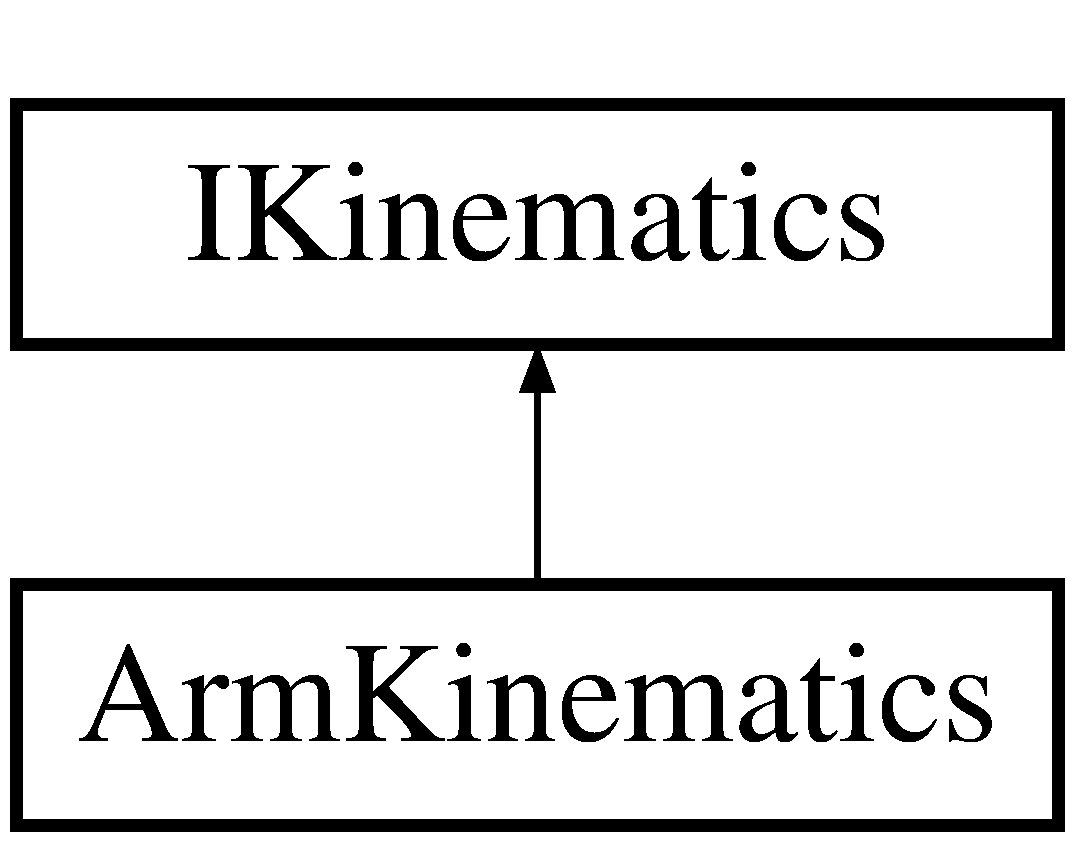
\includegraphics[height=2.000000cm]{classArmKinematics}
\end{center}
\end{figure}
\subsection*{Public Member Functions}
\begin{DoxyCompactItemize}
\item 
\hyperlink{classArmKinematics_a3716ba10905a5f540cfa5dc9030f6eb3}{Arm\-Kinematics} (std\-::string \hyperlink{classIKinematics_a62baaf78436911eca42896cad4b5c911}{prefix}, tf\-::\-Pose \hyperlink{classIKinematics_aa599f7938cbf1c9b422a6d4d50e8e1a9}{baseoffset})
\item 
virtual \hyperlink{namespaceRCS_aa07e45d8a50e30064283d2b38087f999}{R\-C\-S\-::\-Pose} \hyperlink{classArmKinematics_a1773ef10fcdd9bfb7b5d806c42bcbfb1}{F\-K} (std\-::vector$<$ double $>$ jv)
\begin{DoxyCompactList}\small\item\em F\-K performs the forward kinematics using the joint values of the robot provided. \end{DoxyCompactList}\item 
virtual std\-::vector$<$ double $>$ \hyperlink{classArmKinematics_a28e91de4fcb7ae0e8d4ce7d83bef2165}{I\-K} (\hyperlink{namespaceRCS_aa07e45d8a50e30064283d2b38087f999}{R\-C\-S\-::\-Pose} \&pose, std\-::vector$<$ double $>$ oldjoints)
\begin{DoxyCompactList}\small\item\em I\-K performs the inverse kinematics using the Cartesian pose provided. \end{DoxyCompactList}\item 
virtual size\-\_\-t \hyperlink{classArmKinematics_a18053e73102f70dfe7260eafe48b3548}{All\-Pose\-To\-Joints} (\hyperlink{namespaceRCS_aa07e45d8a50e30064283d2b38087f999}{R\-C\-S\-::\-Pose} \&pose, std\-::vector$<$ std\-::vector$<$ double $>$ $>$ \&newjoints)
\begin{DoxyCompactList}\small\item\em All\-Pose\-To\-Joints solves the inverse kinematics to find all solutions using the Cartesian pose provided. \end{DoxyCompactList}\item 
virtual std\-::vector$<$ double $>$ \hyperlink{classArmKinematics_a7836b4724f8036ca171c21b9877b7a7e}{Nearest\-Joints} (std\-::vector$<$ double $>$ oldjoints, std\-::vector$<$ std\-::vector$<$ double $>$ $>$ \&newjoints)
\begin{DoxyCompactList}\small\item\em Nearest\-Joints finds the joint set that is closest to the old joints. \end{DoxyCompactList}\item 
virtual bool \hyperlink{classArmKinematics_af0ef95a582ede450b2bce813340a88cb}{Is\-Singular} (\hyperlink{namespaceRCS_aa07e45d8a50e30064283d2b38087f999}{R\-C\-S\-::\-Pose} \&pose, double threshold)
\begin{DoxyCompactList}\small\item\em Returns true if the determinant of the jacobian is near zero. . \end{DoxyCompactList}\item 
virtual void \hyperlink{classArmKinematics_accebfc031ce46ca59279cca01c152149}{Init} (ros\-::\-Node\-Handle \&nh)
\begin{DoxyCompactList}\small\item\em Initialize kinematics using robot\-\_\-description to fill parameters . \end{DoxyCompactList}\end{DoxyCompactItemize}
\subsection*{Additional Inherited Members}


\subsection{Constructor \& Destructor Documentation}
\hypertarget{classArmKinematics_a3716ba10905a5f540cfa5dc9030f6eb3}{\index{Arm\-Kinematics@{Arm\-Kinematics}!Arm\-Kinematics@{Arm\-Kinematics}}
\index{Arm\-Kinematics@{Arm\-Kinematics}!ArmKinematics@{Arm\-Kinematics}}
\subsubsection[{Arm\-Kinematics}]{\setlength{\rightskip}{0pt plus 5cm}Arm\-Kinematics\-::\-Arm\-Kinematics (
\begin{DoxyParamCaption}
\item[{std\-::string}]{prefix, }
\item[{tf\-::\-Pose}]{baseoffset}
\end{DoxyParamCaption}
)\hspace{0.3cm}{\ttfamily [inline]}}}\label{classArmKinematics_a3716ba10905a5f540cfa5dc9030f6eb3}


\subsection{Member Function Documentation}
\hypertarget{classArmKinematics_a18053e73102f70dfe7260eafe48b3548}{\index{Arm\-Kinematics@{Arm\-Kinematics}!All\-Pose\-To\-Joints@{All\-Pose\-To\-Joints}}
\index{All\-Pose\-To\-Joints@{All\-Pose\-To\-Joints}!ArmKinematics@{Arm\-Kinematics}}
\subsubsection[{All\-Pose\-To\-Joints}]{\setlength{\rightskip}{0pt plus 5cm}virtual size\-\_\-t Arm\-Kinematics\-::\-All\-Pose\-To\-Joints (
\begin{DoxyParamCaption}
\item[{{\bf R\-C\-S\-::\-Pose} \&}]{pose, }
\item[{std\-::vector$<$ std\-::vector$<$ double $>$ $>$ \&}]{newjoints}
\end{DoxyParamCaption}
)\hspace{0.3cm}{\ttfamily [inline]}, {\ttfamily [virtual]}}}\label{classArmKinematics_a18053e73102f70dfe7260eafe48b3548}


All\-Pose\-To\-Joints solves the inverse kinematics to find all solutions using the Cartesian pose provided. 


\begin{DoxyParams}{Parameters}
{\em Cartesian} & robot pose of end effector. \\
\hline
{\em vector} & of double vectos to hold all the I\-K joint solutions. \\
\hline
\end{DoxyParams}
\begin{DoxyReturn}{Returns}
number of solutions found. 
\end{DoxyReturn}


Implements \hyperlink{classIKinematics_aeb53bb4b2a1e70a79d5d724e5eb82c10}{I\-Kinematics}.

\hypertarget{classArmKinematics_a1773ef10fcdd9bfb7b5d806c42bcbfb1}{\index{Arm\-Kinematics@{Arm\-Kinematics}!F\-K@{F\-K}}
\index{F\-K@{F\-K}!ArmKinematics@{Arm\-Kinematics}}
\subsubsection[{F\-K}]{\setlength{\rightskip}{0pt plus 5cm}virtual {\bf R\-C\-S\-::\-Pose} Arm\-Kinematics\-::\-F\-K (
\begin{DoxyParamCaption}
\item[{std\-::vector$<$ double $>$}]{jv}
\end{DoxyParamCaption}
)\hspace{0.3cm}{\ttfamily [inline]}, {\ttfamily [virtual]}}}\label{classArmKinematics_a1773ef10fcdd9bfb7b5d806c42bcbfb1}


F\-K performs the forward kinematics using the joint values of the robot provided. 


\begin{DoxyParams}{Parameters}
{\em vector} & of all robot joint values in doubles. \\
\hline
\end{DoxyParams}
\begin{DoxyReturn}{Returns}
corresponding Cartesian robot pose of end effector. 
\end{DoxyReturn}


Implements \hyperlink{classIKinematics_abf765053ac39fac5b94ef99e80b17f1b}{I\-Kinematics}.

\hypertarget{classArmKinematics_a28e91de4fcb7ae0e8d4ce7d83bef2165}{\index{Arm\-Kinematics@{Arm\-Kinematics}!I\-K@{I\-K}}
\index{I\-K@{I\-K}!ArmKinematics@{Arm\-Kinematics}}
\subsubsection[{I\-K}]{\setlength{\rightskip}{0pt plus 5cm}virtual std\-::vector$<$double$>$ Arm\-Kinematics\-::\-I\-K (
\begin{DoxyParamCaption}
\item[{{\bf R\-C\-S\-::\-Pose} \&}]{pose, }
\item[{std\-::vector$<$ double $>$}]{oldjoints}
\end{DoxyParamCaption}
)\hspace{0.3cm}{\ttfamily [inline]}, {\ttfamily [virtual]}}}\label{classArmKinematics_a28e91de4fcb7ae0e8d4ce7d83bef2165}


I\-K performs the inverse kinematics using the Cartesian pose provided. 


\begin{DoxyParams}{Parameters}
{\em Cartesian} & robot pose of end effector. \\
\hline
{\em optional} & seed joint values to use as best guess for I\-K joint values. \\
\hline
\end{DoxyParams}
\begin{DoxyReturn}{Returns}
vector of all robot joint values in doubles. 
\end{DoxyReturn}


Implements \hyperlink{classIKinematics_ad0715c776a7eb325d2543bc34fa8114f}{I\-Kinematics}.

\hypertarget{classArmKinematics_accebfc031ce46ca59279cca01c152149}{\index{Arm\-Kinematics@{Arm\-Kinematics}!Init@{Init}}
\index{Init@{Init}!ArmKinematics@{Arm\-Kinematics}}
\subsubsection[{Init}]{\setlength{\rightskip}{0pt plus 5cm}virtual void Arm\-Kinematics\-::\-Init (
\begin{DoxyParamCaption}
\item[{ros\-::\-Node\-Handle \&}]{nh}
\end{DoxyParamCaption}
)\hspace{0.3cm}{\ttfamily [inline]}, {\ttfamily [virtual]}}}\label{classArmKinematics_accebfc031ce46ca59279cca01c152149}


Initialize kinematics using robot\-\_\-description to fill parameters . 


\begin{DoxyParams}{Parameters}
{\em nh} & ros node handle of node. \\
\hline
\end{DoxyParams}


Reimplemented from \hyperlink{classIKinematics_aa5c1c9225650b5225f3aa80e06ef1587}{I\-Kinematics}.

\hypertarget{classArmKinematics_af0ef95a582ede450b2bce813340a88cb}{\index{Arm\-Kinematics@{Arm\-Kinematics}!Is\-Singular@{Is\-Singular}}
\index{Is\-Singular@{Is\-Singular}!ArmKinematics@{Arm\-Kinematics}}
\subsubsection[{Is\-Singular}]{\setlength{\rightskip}{0pt plus 5cm}virtual bool Arm\-Kinematics\-::\-Is\-Singular (
\begin{DoxyParamCaption}
\item[{{\bf R\-C\-S\-::\-Pose} \&}]{pose, }
\item[{double}]{threshold}
\end{DoxyParamCaption}
)\hspace{0.3cm}{\ttfamily [inline]}, {\ttfamily [virtual]}}}\label{classArmKinematics_af0ef95a582ede450b2bce813340a88cb}


Returns true if the determinant of the jacobian is near zero. . 


\begin{DoxyParams}{Parameters}
{\em groupname} & name of chained joints in robot model. \\
\hline
{\em eelinkname} & name of end effector joint in robot model. \\
\hline
\end{DoxyParams}


Reimplemented from \hyperlink{classIKinematics_aac7d4f55bbd9228af0a7b733f857fcab}{I\-Kinematics}.

\hypertarget{classArmKinematics_a7836b4724f8036ca171c21b9877b7a7e}{\index{Arm\-Kinematics@{Arm\-Kinematics}!Nearest\-Joints@{Nearest\-Joints}}
\index{Nearest\-Joints@{Nearest\-Joints}!ArmKinematics@{Arm\-Kinematics}}
\subsubsection[{Nearest\-Joints}]{\setlength{\rightskip}{0pt plus 5cm}virtual std\-::vector$<$double$>$ Arm\-Kinematics\-::\-Nearest\-Joints (
\begin{DoxyParamCaption}
\item[{std\-::vector$<$ double $>$}]{oldjoints, }
\item[{std\-::vector$<$ std\-::vector$<$ double $>$ $>$ \&}]{newjoints}
\end{DoxyParamCaption}
)\hspace{0.3cm}{\ttfamily [inline]}, {\ttfamily [virtual]}}}\label{classArmKinematics_a7836b4724f8036ca171c21b9877b7a7e}


Nearest\-Joints finds the joint set that is closest to the old joints. 


\begin{DoxyParams}{Parameters}
{\em old} & seed joint values to use as best guess for I\-K joint values. \\
\hline
{\em vector} & of double vectos that holds all the I\-K joint solutions. \\
\hline
\end{DoxyParams}
\begin{DoxyReturn}{Returns}
vector of doubles with closest set to seed joints. 
\end{DoxyReturn}


Implements \hyperlink{classIKinematics_ab74b70ed6ecc53adfc36505b8dd1fef4}{I\-Kinematics}.



The documentation for this class was generated from the following file\-:\begin{DoxyCompactItemize}
\item 
/usr/local/michalos/nistfanuc\-\_\-ws/src/nist\-\_\-fanuc/include/nist\-\_\-fanuc/\hyperlink{Kinematics_8h}{Kinematics.\-h}\end{DoxyCompactItemize}

\hypertarget{classRCS_1_1BangBangInterpreter}{\section{R\-C\-S\-:\-:Bang\-Bang\-Interpreter Class Reference}
\label{classRCS_1_1BangBangInterpreter}\index{R\-C\-S\-::\-Bang\-Bang\-Interpreter@{R\-C\-S\-::\-Bang\-Bang\-Interpreter}}
}


{\ttfamily \#include $<$R\-C\-S\-Interpreter.\-h$>$}

Inheritance diagram for R\-C\-S\-:\-:Bang\-Bang\-Interpreter\-:\begin{figure}[H]
\begin{center}
\leavevmode
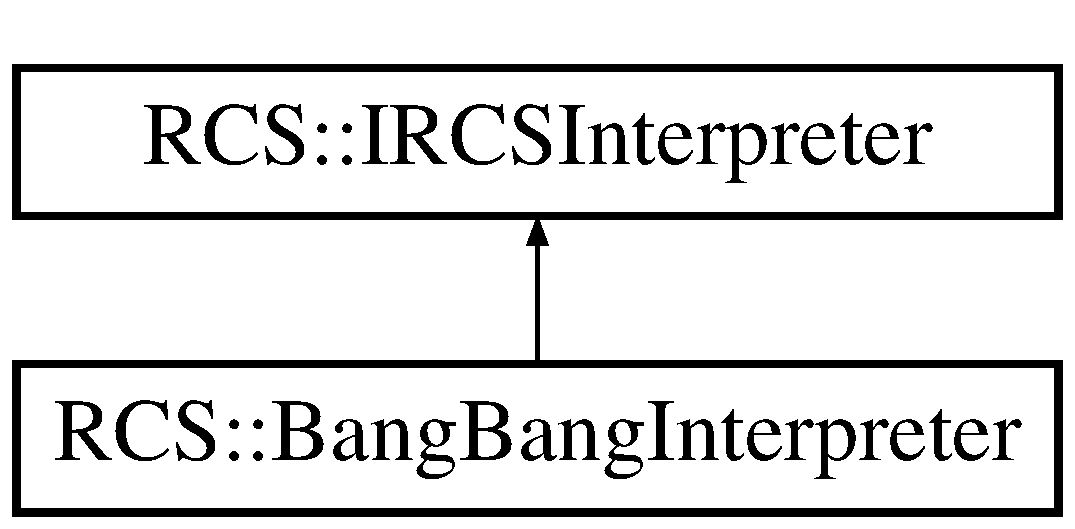
\includegraphics[height=2.000000cm]{classRCS_1_1BangBangInterpreter}
\end{center}
\end{figure}
\subsection*{Public Member Functions}
\begin{DoxyCompactItemize}
\item 
\hyperlink{classRCS_1_1BangBangInterpreter_af5d124c1c3ba7865155018a1f3415695}{Bang\-Bang\-Interpreter} (boost\-::shared\-\_\-ptr$<$ \hyperlink{structRCS_1_1CController}{R\-C\-S\-::\-C\-Controller} $>$ nc, \hyperlink{Kinematics_8h_aa720b9842c846588baf215581fb9f902}{I\-Kinematics\-Shared\-Ptr} k=N\-U\-L\-L)
\item 
virtual \hyperlink{structRCS_1_1CanonCmd}{R\-C\-S\-::\-Canon\-Cmd} \hyperlink{classRCS_1_1BangBangInterpreter_a7a5611f4e162defa15aeb1d503c7f3cb}{Parse\-Command} (\hyperlink{structRCS_1_1CanonCmd}{R\-C\-S\-::\-Canon\-Cmd} cmd)
\item 
virtual void \hyperlink{classRCS_1_1BangBangInterpreter_a69cc779236827f55ff895019e4833209}{Set\-Range} (std\-::vector$<$ double $>$ \hyperlink{classRCS_1_1BangBangInterpreter_a83562103bf03ffe4de00cd3a2f06c772}{minrange}, std\-::vector$<$ double $>$ \hyperlink{classRCS_1_1BangBangInterpreter_a4e10b3c84dfeb87228da9eb62be855c0}{maxrange})
\end{DoxyCompactItemize}
\subsection*{Public Attributes}
\begin{DoxyCompactItemize}
\item 
std\-::vector$<$ double $>$ \hyperlink{classRCS_1_1BangBangInterpreter_a83562103bf03ffe4de00cd3a2f06c772}{minrange}
\item 
std\-::vector$<$ double $>$ \hyperlink{classRCS_1_1BangBangInterpreter_a4e10b3c84dfeb87228da9eb62be855c0}{maxrange}
\end{DoxyCompactItemize}
\subsection*{Protected Attributes}
\begin{DoxyCompactItemize}
\item 
\hyperlink{Kinematics_8h_aa720b9842c846588baf215581fb9f902}{I\-Kinematics\-Shared\-Ptr} \hyperlink{classRCS_1_1BangBangInterpreter_a3c3c12685416ba957ce2176c062890b4}{\-\_\-kinematics}
\item 
boost\-::shared\-\_\-ptr\\*
$<$ \hyperlink{structRCS_1_1CController}{R\-C\-S\-::\-C\-Controller} $>$ \hyperlink{classRCS_1_1BangBangInterpreter_a874d893a4134087ff5493758661599e2}{\-\_\-nc}
\end{DoxyCompactItemize}


\subsection{Constructor \& Destructor Documentation}
\hypertarget{classRCS_1_1BangBangInterpreter_af5d124c1c3ba7865155018a1f3415695}{\index{R\-C\-S\-::\-Bang\-Bang\-Interpreter@{R\-C\-S\-::\-Bang\-Bang\-Interpreter}!Bang\-Bang\-Interpreter@{Bang\-Bang\-Interpreter}}
\index{Bang\-Bang\-Interpreter@{Bang\-Bang\-Interpreter}!RCS::BangBangInterpreter@{R\-C\-S\-::\-Bang\-Bang\-Interpreter}}
\subsubsection[{Bang\-Bang\-Interpreter}]{\setlength{\rightskip}{0pt plus 5cm}Bang\-Bang\-Interpreter\-::\-Bang\-Bang\-Interpreter (
\begin{DoxyParamCaption}
\item[{boost\-::shared\-\_\-ptr$<$ {\bf R\-C\-S\-::\-C\-Controller} $>$}]{nc, }
\item[{{\bf I\-Kinematics\-Shared\-Ptr}}]{k = {\ttfamily NULL}}
\end{DoxyParamCaption}
)}}\label{classRCS_1_1BangBangInterpreter_af5d124c1c3ba7865155018a1f3415695}
uint8 crclcommand

\subsection*{\href{https://github.com/ros/common_msgs}{\tt https\-://github.\-com/ros/common\-\_\-msgs}}

geometry\-\_\-msgs/\-Pose finalpose geometry\-\_\-msgs/\-Pose\mbox{[}\mbox{]} waypoints \subsection*{Below joint info could be trajectory\-\_\-msgs/\-Joint\-Trajectory\-Point}

sensor\-\_\-msgs/\-Joint\-State joints bool b\-Straight float64 dwell\-\_\-seconds string opmessage bool b\-Coordinated float64 eepercent Crcl\-Max\-Profile\-Msg\mbox{[}\mbox{]} profile \# maximum profile 

\subsection{Member Function Documentation}
\hypertarget{classRCS_1_1BangBangInterpreter_a7a5611f4e162defa15aeb1d503c7f3cb}{\index{R\-C\-S\-::\-Bang\-Bang\-Interpreter@{R\-C\-S\-::\-Bang\-Bang\-Interpreter}!Parse\-Command@{Parse\-Command}}
\index{Parse\-Command@{Parse\-Command}!RCS::BangBangInterpreter@{R\-C\-S\-::\-Bang\-Bang\-Interpreter}}
\subsubsection[{Parse\-Command}]{\setlength{\rightskip}{0pt plus 5cm}{\bf R\-C\-S\-::\-Canon\-Cmd} Bang\-Bang\-Interpreter\-::\-Parse\-Command (
\begin{DoxyParamCaption}
\item[{{\bf R\-C\-S\-::\-Canon\-Cmd}}]{cmd}
\end{DoxyParamCaption}
)\hspace{0.3cm}{\ttfamily [virtual]}}}\label{classRCS_1_1BangBangInterpreter_a7a5611f4e162defa15aeb1d503c7f3cb}


Implements \hyperlink{classRCS_1_1IRCSInterpreter_adb4258abff48650cc30398ec996d04c1}{R\-C\-S\-::\-I\-R\-C\-S\-Interpreter}.

\hypertarget{classRCS_1_1BangBangInterpreter_a69cc779236827f55ff895019e4833209}{\index{R\-C\-S\-::\-Bang\-Bang\-Interpreter@{R\-C\-S\-::\-Bang\-Bang\-Interpreter}!Set\-Range@{Set\-Range}}
\index{Set\-Range@{Set\-Range}!RCS::BangBangInterpreter@{R\-C\-S\-::\-Bang\-Bang\-Interpreter}}
\subsubsection[{Set\-Range}]{\setlength{\rightskip}{0pt plus 5cm}void Bang\-Bang\-Interpreter\-::\-Set\-Range (
\begin{DoxyParamCaption}
\item[{std\-::vector$<$ double $>$}]{minrange, }
\item[{std\-::vector$<$ double $>$}]{maxrange}
\end{DoxyParamCaption}
)\hspace{0.3cm}{\ttfamily [virtual]}}}\label{classRCS_1_1BangBangInterpreter_a69cc779236827f55ff895019e4833209}


Reimplemented from \hyperlink{classRCS_1_1IRCSInterpreter_a5181a696aed581ae842bfd31537cfc1f}{R\-C\-S\-::\-I\-R\-C\-S\-Interpreter}.



\subsection{Member Data Documentation}
\hypertarget{classRCS_1_1BangBangInterpreter_a3c3c12685416ba957ce2176c062890b4}{\index{R\-C\-S\-::\-Bang\-Bang\-Interpreter@{R\-C\-S\-::\-Bang\-Bang\-Interpreter}!\-\_\-kinematics@{\-\_\-kinematics}}
\index{\-\_\-kinematics@{\-\_\-kinematics}!RCS::BangBangInterpreter@{R\-C\-S\-::\-Bang\-Bang\-Interpreter}}
\subsubsection[{\-\_\-kinematics}]{\setlength{\rightskip}{0pt plus 5cm}{\bf I\-Kinematics\-Shared\-Ptr} R\-C\-S\-::\-Bang\-Bang\-Interpreter\-::\-\_\-kinematics\hspace{0.3cm}{\ttfamily [protected]}}}\label{classRCS_1_1BangBangInterpreter_a3c3c12685416ba957ce2176c062890b4}
kinematics pointer \hypertarget{classRCS_1_1BangBangInterpreter_a874d893a4134087ff5493758661599e2}{\index{R\-C\-S\-::\-Bang\-Bang\-Interpreter@{R\-C\-S\-::\-Bang\-Bang\-Interpreter}!\-\_\-nc@{\-\_\-nc}}
\index{\-\_\-nc@{\-\_\-nc}!RCS::BangBangInterpreter@{R\-C\-S\-::\-Bang\-Bang\-Interpreter}}
\subsubsection[{\-\_\-nc}]{\setlength{\rightskip}{0pt plus 5cm}boost\-::shared\-\_\-ptr$<${\bf R\-C\-S\-::\-C\-Controller}$>$ R\-C\-S\-::\-Bang\-Bang\-Interpreter\-::\-\_\-nc\hspace{0.3cm}{\ttfamily [protected]}}}\label{classRCS_1_1BangBangInterpreter_a874d893a4134087ff5493758661599e2}
\hypertarget{classRCS_1_1BangBangInterpreter_a4e10b3c84dfeb87228da9eb62be855c0}{\index{R\-C\-S\-::\-Bang\-Bang\-Interpreter@{R\-C\-S\-::\-Bang\-Bang\-Interpreter}!maxrange@{maxrange}}
\index{maxrange@{maxrange}!RCS::BangBangInterpreter@{R\-C\-S\-::\-Bang\-Bang\-Interpreter}}
\subsubsection[{maxrange}]{\setlength{\rightskip}{0pt plus 5cm}std\-::vector$<$double$>$ R\-C\-S\-::\-Bang\-Bang\-Interpreter\-::maxrange}}\label{classRCS_1_1BangBangInterpreter_a4e10b3c84dfeb87228da9eb62be855c0}
\hypertarget{classRCS_1_1BangBangInterpreter_a83562103bf03ffe4de00cd3a2f06c772}{\index{R\-C\-S\-::\-Bang\-Bang\-Interpreter@{R\-C\-S\-::\-Bang\-Bang\-Interpreter}!minrange@{minrange}}
\index{minrange@{minrange}!RCS::BangBangInterpreter@{R\-C\-S\-::\-Bang\-Bang\-Interpreter}}
\subsubsection[{minrange}]{\setlength{\rightskip}{0pt plus 5cm}std\-::vector$<$double$>$ R\-C\-S\-::\-Bang\-Bang\-Interpreter\-::minrange}}\label{classRCS_1_1BangBangInterpreter_a83562103bf03ffe4de00cd3a2f06c772}


The documentation for this class was generated from the following files\-:\begin{DoxyCompactItemize}
\item 
/usr/local/michalos/nistfanuc\-\_\-ws/src/nist\-\_\-fanuc/include/nist\-\_\-fanuc/\hyperlink{RCSInterpreter_8h}{R\-C\-S\-Interpreter.\-h}\item 
/usr/local/michalos/nistfanuc\-\_\-ws/src/nist\-\_\-fanuc/src/\hyperlink{RCSInterpreter_8cpp}{R\-C\-S\-Interpreter.\-cpp}\end{DoxyCompactItemize}

\hypertarget{structCheckers_1_1BoardType}{\section{Checkers\-:\-:Board\-Type Struct Reference}
\label{structCheckers_1_1BoardType}\index{Checkers\-::\-Board\-Type@{Checkers\-::\-Board\-Type}}
}


{\ttfamily \#include $<$Checkers.\-h$>$}

Inheritance diagram for Checkers\-:\-:Board\-Type\-:\begin{figure}[H]
\begin{center}
\leavevmode
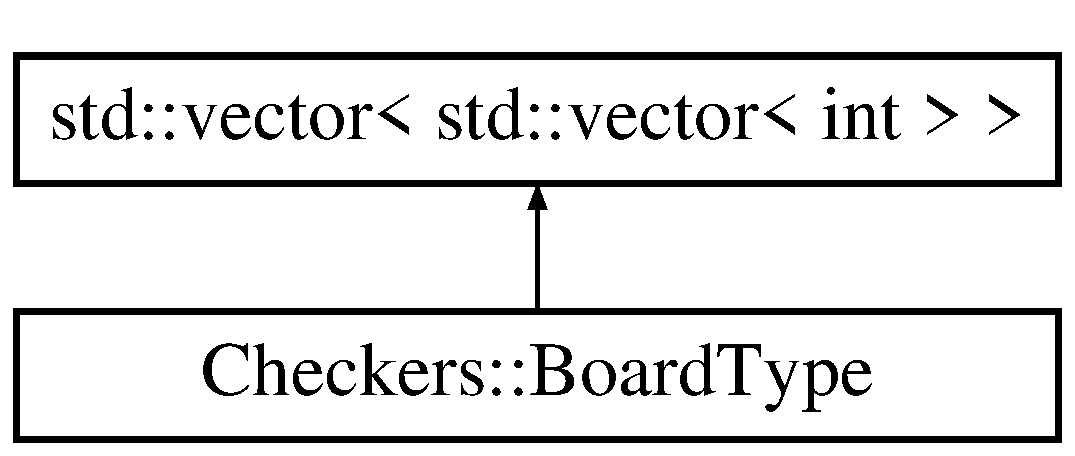
\includegraphics[height=2.000000cm]{structCheckers_1_1BoardType}
\end{center}
\end{figure}
\subsection*{Public Member Functions}
\begin{DoxyCompactItemize}
\item 
\hyperlink{structCheckers_1_1BoardType_a9314173d6d113003665c6f04e2f65ca1}{Board\-Type} ()
\end{DoxyCompactItemize}


\subsection{Constructor \& Destructor Documentation}
\hypertarget{structCheckers_1_1BoardType_a9314173d6d113003665c6f04e2f65ca1}{\index{Checkers\-::\-Board\-Type@{Checkers\-::\-Board\-Type}!Board\-Type@{Board\-Type}}
\index{Board\-Type@{Board\-Type}!Checkers::BoardType@{Checkers\-::\-Board\-Type}}
\subsubsection[{Board\-Type}]{\setlength{\rightskip}{0pt plus 5cm}Checkers\-::\-Board\-Type\-::\-Board\-Type (
\begin{DoxyParamCaption}
{}
\end{DoxyParamCaption}
)\hspace{0.3cm}{\ttfamily [inline]}}}\label{structCheckers_1_1BoardType_a9314173d6d113003665c6f04e2f65ca1}


The documentation for this struct was generated from the following file\-:\begin{DoxyCompactItemize}
\item 
/usr/local/michalos/nistfanuc\-\_\-ws/src/nist\-\_\-fanuc/include/nist\-\_\-fanuc/\hyperlink{Checkers_8h}{Checkers.\-h}\end{DoxyCompactItemize}

\hypertarget{structRCS_1_1CanonAccProfile}{\section{R\-C\-S\-:\-:Canon\-Acc\-Profile Struct Reference}
\label{structRCS_1_1CanonAccProfile}\index{R\-C\-S\-::\-Canon\-Acc\-Profile@{R\-C\-S\-::\-Canon\-Acc\-Profile}}
}


enumeration of trajectory acceleration profile.  




{\ttfamily \#include $<$R\-C\-S.\-h$>$}

\subsection*{Static Public Attributes}
\begin{DoxyCompactItemize}
\item 
static const int \hyperlink{structRCS_1_1CanonAccProfile_a4c8249dfd6aaf09367d2abf3a2c6f54e}{M\-S\-\_\-\-I\-S\-\_\-\-U\-N\-S\-E\-T} = 0
\item 
static const int \hyperlink{structRCS_1_1CanonAccProfile_a24163f7b52c122d7329acb7f848c5587}{M\-S\-\_\-\-I\-S\-\_\-\-D\-O\-N\-E} = 1
\item 
static const int \hyperlink{structRCS_1_1CanonAccProfile_ada8d9c411cbff5e10fb811a994f390ba}{M\-S\-\_\-\-I\-S\-\_\-\-A\-C\-C\-E\-L} = 2
\item 
static const int \hyperlink{structRCS_1_1CanonAccProfile_a38dff6ea9c20f5798ef873747cdd9a7f}{M\-S\-\_\-\-I\-S\-\_\-\-C\-O\-N\-S\-T} = 3
\item 
static const int \hyperlink{structRCS_1_1CanonAccProfile_ac58e66a5af8c68f4c1da483da6c35166}{M\-S\-\_\-\-I\-S\-\_\-\-D\-E\-C\-E\-L} = 4
\item 
static const int \hyperlink{structRCS_1_1CanonAccProfile_a666610a5efde57705413ef2dd65e1fb4}{M\-S\-\_\-\-I\-S\-\_\-\-E\-S\-T\-O\-P\-P\-I\-N\-G} = 5
\item 
static const int \hyperlink{structRCS_1_1CanonAccProfile_a83cd5d24039e517647d72a6a9c82afe3}{M\-S\-\_\-\-I\-S\-\_\-\-P\-A\-U\-S\-E\-D} = 6
\end{DoxyCompactItemize}


\subsection{Detailed Description}
enumeration of trajectory acceleration profile. 

\subsection{Member Data Documentation}
\hypertarget{structRCS_1_1CanonAccProfile_ada8d9c411cbff5e10fb811a994f390ba}{\index{R\-C\-S\-::\-Canon\-Acc\-Profile@{R\-C\-S\-::\-Canon\-Acc\-Profile}!M\-S\-\_\-\-I\-S\-\_\-\-A\-C\-C\-E\-L@{M\-S\-\_\-\-I\-S\-\_\-\-A\-C\-C\-E\-L}}
\index{M\-S\-\_\-\-I\-S\-\_\-\-A\-C\-C\-E\-L@{M\-S\-\_\-\-I\-S\-\_\-\-A\-C\-C\-E\-L}!RCS::CanonAccProfile@{R\-C\-S\-::\-Canon\-Acc\-Profile}}
\subsubsection[{M\-S\-\_\-\-I\-S\-\_\-\-A\-C\-C\-E\-L}]{\setlength{\rightskip}{0pt plus 5cm}const int R\-C\-S\-::\-Canon\-Acc\-Profile\-::\-M\-S\-\_\-\-I\-S\-\_\-\-A\-C\-C\-E\-L = 2\hspace{0.3cm}{\ttfamily [static]}}}\label{structRCS_1_1CanonAccProfile_ada8d9c411cbff5e10fb811a994f390ba}
\hypertarget{structRCS_1_1CanonAccProfile_a38dff6ea9c20f5798ef873747cdd9a7f}{\index{R\-C\-S\-::\-Canon\-Acc\-Profile@{R\-C\-S\-::\-Canon\-Acc\-Profile}!M\-S\-\_\-\-I\-S\-\_\-\-C\-O\-N\-S\-T@{M\-S\-\_\-\-I\-S\-\_\-\-C\-O\-N\-S\-T}}
\index{M\-S\-\_\-\-I\-S\-\_\-\-C\-O\-N\-S\-T@{M\-S\-\_\-\-I\-S\-\_\-\-C\-O\-N\-S\-T}!RCS::CanonAccProfile@{R\-C\-S\-::\-Canon\-Acc\-Profile}}
\subsubsection[{M\-S\-\_\-\-I\-S\-\_\-\-C\-O\-N\-S\-T}]{\setlength{\rightskip}{0pt plus 5cm}const int R\-C\-S\-::\-Canon\-Acc\-Profile\-::\-M\-S\-\_\-\-I\-S\-\_\-\-C\-O\-N\-S\-T = 3\hspace{0.3cm}{\ttfamily [static]}}}\label{structRCS_1_1CanonAccProfile_a38dff6ea9c20f5798ef873747cdd9a7f}
\hypertarget{structRCS_1_1CanonAccProfile_ac58e66a5af8c68f4c1da483da6c35166}{\index{R\-C\-S\-::\-Canon\-Acc\-Profile@{R\-C\-S\-::\-Canon\-Acc\-Profile}!M\-S\-\_\-\-I\-S\-\_\-\-D\-E\-C\-E\-L@{M\-S\-\_\-\-I\-S\-\_\-\-D\-E\-C\-E\-L}}
\index{M\-S\-\_\-\-I\-S\-\_\-\-D\-E\-C\-E\-L@{M\-S\-\_\-\-I\-S\-\_\-\-D\-E\-C\-E\-L}!RCS::CanonAccProfile@{R\-C\-S\-::\-Canon\-Acc\-Profile}}
\subsubsection[{M\-S\-\_\-\-I\-S\-\_\-\-D\-E\-C\-E\-L}]{\setlength{\rightskip}{0pt plus 5cm}const int R\-C\-S\-::\-Canon\-Acc\-Profile\-::\-M\-S\-\_\-\-I\-S\-\_\-\-D\-E\-C\-E\-L = 4\hspace{0.3cm}{\ttfamily [static]}}}\label{structRCS_1_1CanonAccProfile_ac58e66a5af8c68f4c1da483da6c35166}
\hypertarget{structRCS_1_1CanonAccProfile_a24163f7b52c122d7329acb7f848c5587}{\index{R\-C\-S\-::\-Canon\-Acc\-Profile@{R\-C\-S\-::\-Canon\-Acc\-Profile}!M\-S\-\_\-\-I\-S\-\_\-\-D\-O\-N\-E@{M\-S\-\_\-\-I\-S\-\_\-\-D\-O\-N\-E}}
\index{M\-S\-\_\-\-I\-S\-\_\-\-D\-O\-N\-E@{M\-S\-\_\-\-I\-S\-\_\-\-D\-O\-N\-E}!RCS::CanonAccProfile@{R\-C\-S\-::\-Canon\-Acc\-Profile}}
\subsubsection[{M\-S\-\_\-\-I\-S\-\_\-\-D\-O\-N\-E}]{\setlength{\rightskip}{0pt plus 5cm}const int R\-C\-S\-::\-Canon\-Acc\-Profile\-::\-M\-S\-\_\-\-I\-S\-\_\-\-D\-O\-N\-E = 1\hspace{0.3cm}{\ttfamily [static]}}}\label{structRCS_1_1CanonAccProfile_a24163f7b52c122d7329acb7f848c5587}
\hypertarget{structRCS_1_1CanonAccProfile_a666610a5efde57705413ef2dd65e1fb4}{\index{R\-C\-S\-::\-Canon\-Acc\-Profile@{R\-C\-S\-::\-Canon\-Acc\-Profile}!M\-S\-\_\-\-I\-S\-\_\-\-E\-S\-T\-O\-P\-P\-I\-N\-G@{M\-S\-\_\-\-I\-S\-\_\-\-E\-S\-T\-O\-P\-P\-I\-N\-G}}
\index{M\-S\-\_\-\-I\-S\-\_\-\-E\-S\-T\-O\-P\-P\-I\-N\-G@{M\-S\-\_\-\-I\-S\-\_\-\-E\-S\-T\-O\-P\-P\-I\-N\-G}!RCS::CanonAccProfile@{R\-C\-S\-::\-Canon\-Acc\-Profile}}
\subsubsection[{M\-S\-\_\-\-I\-S\-\_\-\-E\-S\-T\-O\-P\-P\-I\-N\-G}]{\setlength{\rightskip}{0pt plus 5cm}const int R\-C\-S\-::\-Canon\-Acc\-Profile\-::\-M\-S\-\_\-\-I\-S\-\_\-\-E\-S\-T\-O\-P\-P\-I\-N\-G = 5\hspace{0.3cm}{\ttfamily [static]}}}\label{structRCS_1_1CanonAccProfile_a666610a5efde57705413ef2dd65e1fb4}
\hypertarget{structRCS_1_1CanonAccProfile_a83cd5d24039e517647d72a6a9c82afe3}{\index{R\-C\-S\-::\-Canon\-Acc\-Profile@{R\-C\-S\-::\-Canon\-Acc\-Profile}!M\-S\-\_\-\-I\-S\-\_\-\-P\-A\-U\-S\-E\-D@{M\-S\-\_\-\-I\-S\-\_\-\-P\-A\-U\-S\-E\-D}}
\index{M\-S\-\_\-\-I\-S\-\_\-\-P\-A\-U\-S\-E\-D@{M\-S\-\_\-\-I\-S\-\_\-\-P\-A\-U\-S\-E\-D}!RCS::CanonAccProfile@{R\-C\-S\-::\-Canon\-Acc\-Profile}}
\subsubsection[{M\-S\-\_\-\-I\-S\-\_\-\-P\-A\-U\-S\-E\-D}]{\setlength{\rightskip}{0pt plus 5cm}const int R\-C\-S\-::\-Canon\-Acc\-Profile\-::\-M\-S\-\_\-\-I\-S\-\_\-\-P\-A\-U\-S\-E\-D = 6\hspace{0.3cm}{\ttfamily [static]}}}\label{structRCS_1_1CanonAccProfile_a83cd5d24039e517647d72a6a9c82afe3}
\hypertarget{structRCS_1_1CanonAccProfile_a4c8249dfd6aaf09367d2abf3a2c6f54e}{\index{R\-C\-S\-::\-Canon\-Acc\-Profile@{R\-C\-S\-::\-Canon\-Acc\-Profile}!M\-S\-\_\-\-I\-S\-\_\-\-U\-N\-S\-E\-T@{M\-S\-\_\-\-I\-S\-\_\-\-U\-N\-S\-E\-T}}
\index{M\-S\-\_\-\-I\-S\-\_\-\-U\-N\-S\-E\-T@{M\-S\-\_\-\-I\-S\-\_\-\-U\-N\-S\-E\-T}!RCS::CanonAccProfile@{R\-C\-S\-::\-Canon\-Acc\-Profile}}
\subsubsection[{M\-S\-\_\-\-I\-S\-\_\-\-U\-N\-S\-E\-T}]{\setlength{\rightskip}{0pt plus 5cm}const int R\-C\-S\-::\-Canon\-Acc\-Profile\-::\-M\-S\-\_\-\-I\-S\-\_\-\-U\-N\-S\-E\-T = 0\hspace{0.3cm}{\ttfamily [static]}}}\label{structRCS_1_1CanonAccProfile_a4c8249dfd6aaf09367d2abf3a2c6f54e}


The documentation for this struct was generated from the following file\-:\begin{DoxyCompactItemize}
\item 
/usr/local/michalos/nistfanuc\-\_\-ws/src/nist\-\_\-fanuc/include/nist\-\_\-fanuc/\hyperlink{RCS_8h}{R\-C\-S.\-h}\end{DoxyCompactItemize}

\hypertarget{structRCS_1_1CanonAngleUnit}{\section{R\-C\-S\-:\-:Canon\-Angle\-Unit Struct Reference}
\label{structRCS_1_1CanonAngleUnit}\index{R\-C\-S\-::\-Canon\-Angle\-Unit@{R\-C\-S\-::\-Canon\-Angle\-Unit}}
}


enumeration of angle units. \hyperlink{namespaceConversion}{Conversion} into R\-O\-S compatible radians.  




{\ttfamily \#include $<$R\-C\-S.\-h$>$}

\subsection*{Static Public Attributes}
\begin{DoxyCompactItemize}
\item 
static const int \hyperlink{structRCS_1_1CanonAngleUnit_a2ce063b43cdf08df392c41de9918bb78}{R\-A\-D\-I\-A\-N} = 0
\item 
static const int \hyperlink{structRCS_1_1CanonAngleUnit_a4b3cdd4b5b779ab93d39a83af474556b}{D\-E\-G\-R\-E\-E} = 1
\end{DoxyCompactItemize}


\subsection{Detailed Description}
enumeration of angle units. \hyperlink{namespaceConversion}{Conversion} into R\-O\-S compatible radians. 

\subsection{Member Data Documentation}
\hypertarget{structRCS_1_1CanonAngleUnit_a4b3cdd4b5b779ab93d39a83af474556b}{\index{R\-C\-S\-::\-Canon\-Angle\-Unit@{R\-C\-S\-::\-Canon\-Angle\-Unit}!D\-E\-G\-R\-E\-E@{D\-E\-G\-R\-E\-E}}
\index{D\-E\-G\-R\-E\-E@{D\-E\-G\-R\-E\-E}!RCS::CanonAngleUnit@{R\-C\-S\-::\-Canon\-Angle\-Unit}}
\subsubsection[{D\-E\-G\-R\-E\-E}]{\setlength{\rightskip}{0pt plus 5cm}const int R\-C\-S\-::\-Canon\-Angle\-Unit\-::\-D\-E\-G\-R\-E\-E = 1\hspace{0.3cm}{\ttfamily [static]}}}\label{structRCS_1_1CanonAngleUnit_a4b3cdd4b5b779ab93d39a83af474556b}
\hypertarget{structRCS_1_1CanonAngleUnit_a2ce063b43cdf08df392c41de9918bb78}{\index{R\-C\-S\-::\-Canon\-Angle\-Unit@{R\-C\-S\-::\-Canon\-Angle\-Unit}!R\-A\-D\-I\-A\-N@{R\-A\-D\-I\-A\-N}}
\index{R\-A\-D\-I\-A\-N@{R\-A\-D\-I\-A\-N}!RCS::CanonAngleUnit@{R\-C\-S\-::\-Canon\-Angle\-Unit}}
\subsubsection[{R\-A\-D\-I\-A\-N}]{\setlength{\rightskip}{0pt plus 5cm}const int R\-C\-S\-::\-Canon\-Angle\-Unit\-::\-R\-A\-D\-I\-A\-N = 0\hspace{0.3cm}{\ttfamily [static]}}}\label{structRCS_1_1CanonAngleUnit_a2ce063b43cdf08df392c41de9918bb78}


The documentation for this struct was generated from the following file\-:\begin{DoxyCompactItemize}
\item 
/usr/local/michalos/nistfanuc\-\_\-ws/src/nist\-\_\-fanuc/include/nist\-\_\-fanuc/\hyperlink{RCS_8h}{R\-C\-S.\-h}\end{DoxyCompactItemize}

\hypertarget{structRCS_1_1CanonCmd}{\section{R\-C\-S\-:\-:Canon\-Cmd Struct Reference}
\label{structRCS_1_1CanonCmd}\index{R\-C\-S\-::\-Canon\-Cmd@{R\-C\-S\-::\-Canon\-Cmd}}
}


\hyperlink{structRCS_1_1CanonCmd}{Canon\-Cmd} is the controller command structure.  




{\ttfamily \#include $<$R\-C\-S.\-h$>$}

\subsection*{Public Member Functions}
\begin{DoxyCompactItemize}
\item 
\hyperlink{structRCS_1_1CanonCmd_a29c997874838bcca02aea1200bb785eb}{Canon\-Cmd} ()
\begin{DoxyCompactList}\small\item\em \hyperlink{structRCS_1_1CanonCmd}{Canon\-Cmd} constructor. \end{DoxyCompactList}\item 
void \hyperlink{structRCS_1_1CanonCmd_acc6132ab423f9349c970785d9f06d542}{Init} ()
\item 
\hyperlink{structRCS_1_1CanonCmd_a493a750837dc6e140e218f4d800faf72}{V\-A\-R} (Command\-I\-D, unsigned long long)
\item 
\hyperlink{structRCS_1_1CanonCmd_a052f3e27333e03886a95a7844e92b71c}{V\-A\-R} (Parent\-Command\-I\-D, unsigned long long)
\item 
\hyperlink{structRCS_1_1CanonCmd_a38899ecf42f1c5ca2921508dea054e3e}{V\-A\-R} (Status\-I\-D, unsigned long long)
\item 
\hyperlink{structRCS_1_1CanonCmd_aefa3700ebd88b157b3975c39d69b0edf}{V\-A\-R} (Rates, \hyperlink{classRCS_1_1IRate}{I\-Rate})
\item 
bool \hyperlink{structRCS_1_1CanonCmd_ab316e8d36adcebbe7b315cb1ed5fe86b}{Is\-Motion\-Cmd} ()
\end{DoxyCompactItemize}
\subsection*{Public Attributes}
\begin{DoxyCompactItemize}
\item 
\hyperlink{namespaceRCS_a55bbd74afb87a330de1b95af65f4cb75}{Canon\-Cmd\-Type} \hyperlink{structRCS_1_1CanonCmd_abf4d78b8604ce73d23d58f1fdcd7305e}{cmd}
\item 
\hyperlink{namespaceRCS_a0e720341c250145b8a2bbf6a1afa777d}{Canon\-Status\-Type} \hyperlink{structRCS_1_1CanonCmd_a8ad6bd631d2cf99c00ec267791680236}{status}
\item 
\hyperlink{namespaceRCS_ae705dbb4b887b18fef40316b6d5ca2c9}{Traj\-Point\-Type} \hyperlink{structRCS_1_1CanonCmd_abf1d51c90a3f1b4c5796292c53cbde01}{type}
\item 
\hyperlink{namespaceRCS_a39ae96212f304024b5f91fe8d63a40c0}{Canon\-Stop\-Motion\-Type} \hyperlink{structRCS_1_1CanonCmd_a22bc418b884c7afabf0a2d3538f74cad}{stoptype}
\item 
bool \hyperlink{structRCS_1_1CanonCmd_abae89c19f08f9011d6e5d3f86e8b6df9}{b\-Coordinated}
\item 
bool \hyperlink{structRCS_1_1CanonCmd_aee8ba85725943aa0102f3305a1bce2a7}{b\-Straight}
\item 
double \hyperlink{structRCS_1_1CanonCmd_a129e91d931073194c3baaed83f56373e}{abs\-Trans\-Acc}
\item 
double \hyperlink{structRCS_1_1CanonCmd_abac67431174c72bbc8bc1e14916cba60}{abs\-Trans\-Speed}
\item 
double \hyperlink{structRCS_1_1CanonCmd_ae1abe3a2d6c4c54776ad46738b3bf571}{abs\-Rot\-Acc}
\item 
double \hyperlink{structRCS_1_1CanonCmd_ad7ce99c4f8d61314aef30c376ace79b7}{abs\-Rot\-Speed}
\item 
double \hyperlink{structRCS_1_1CanonCmd_ac31a9f71e4cbf531255df37780deed05}{abs\-Joint\-Acc}
\item 
double \hyperlink{structRCS_1_1CanonCmd_a0af201b279565849516543a913f443f7}{abs\-Joint\-Speed}
\item 
double \hyperlink{structRCS_1_1CanonCmd_a842c88485db006b71c7653e2a2159233}{dwell}
\item 
double \hyperlink{structRCS_1_1CanonCmd_a03e23d97c74abd3c6b5b38aec8ae5fc2}{gripper\-Pos}
\item 
\hyperlink{namespaceRCS_a452a9217023e577031dcdf7e533b2ead}{Canon\-Acc\-Profile} \hyperlink{structRCS_1_1CanonCmd_a29d47510cc8f459cfa085ef9123bef22}{accprofile}
\item 
std\-::vector$<$ double $>$ \hyperlink{structRCS_1_1CanonCmd_aa31954bd04399469490123786ee17496}{speed}
\item 
std\-::vector$<$ int $>$ \hyperlink{structRCS_1_1CanonCmd_a1fb8395cab4ebddddafd37e7387f9ff8}{jointnum}
\item 
\hyperlink{RCS_8h_aa4adb93a26caa4dacba9c9614e283245}{Joint\-State} \hyperlink{structRCS_1_1CanonCmd_aca799c5c818f28f0d9f4797b325b03de}{joints}
\item 
\hyperlink{RCS_8h_aa4adb93a26caa4dacba9c9614e283245}{Joint\-State} \hyperlink{structRCS_1_1CanonCmd_a577caa222abd73e6490108c7aecbc61c}{seed}
\item 
\hyperlink{namespaceRCS_aa07e45d8a50e30064283d2b38087f999}{R\-C\-S\-::\-Pose} \hyperlink{structRCS_1_1CanonCmd_adc27ad3ae01d7aab1c9c92f08df82fc1}{pose}
\item 
\hyperlink{namespaceRCS_aa07e45d8a50e30064283d2b38087f999}{R\-C\-S\-::\-Pose} \hyperlink{structRCS_1_1CanonCmd_a11e66454d05007664d63cea7b35822c2}{end\-Pose\-Tol}
\item 
std\-::vector$<$ \hyperlink{namespaceRCS_aa07e45d8a50e30064283d2b38087f999}{R\-C\-S\-::\-Pose} $>$ \hyperlink{structRCS_1_1CanonCmd_a1f7fdffabe34bcb3f0afd42f60040648}{waypoints}
\item 
\hyperlink{namespaceRCS_aa07e45d8a50e30064283d2b38087f999}{R\-C\-S\-::\-Pose} \hyperlink{structRCS_1_1CanonCmd_a9b27fcbd1298ee6a95e412a68741ddfc}{intermediate\-Pt\-Tol}
\item 
\hyperlink{namespaceRCS_aa07e45d8a50e30064283d2b38087f999}{R\-C\-S\-::\-Pose} \hyperlink{structRCS_1_1CanonCmd_af76b1a60d2d7282d1a60863c907176de}{gripper\-Tol}
\end{DoxyCompactItemize}
\subsection*{Static Public Attributes}
\begin{DoxyCompactItemize}
\item 
static unsigned long long \hyperlink{structRCS_1_1CanonCmd_ae719b5ae5d58e75b652b27df76113010}{\-\_\-cmdid} = 0
\end{DoxyCompactItemize}


\subsection{Detailed Description}
\hyperlink{structRCS_1_1CanonCmd}{Canon\-Cmd} is the controller command structure. 

\subsection{Constructor \& Destructor Documentation}
\hypertarget{structRCS_1_1CanonCmd_a29c997874838bcca02aea1200bb785eb}{\index{R\-C\-S\-::\-Canon\-Cmd@{R\-C\-S\-::\-Canon\-Cmd}!Canon\-Cmd@{Canon\-Cmd}}
\index{Canon\-Cmd@{Canon\-Cmd}!RCS::CanonCmd@{R\-C\-S\-::\-Canon\-Cmd}}
\subsubsection[{Canon\-Cmd}]{\setlength{\rightskip}{0pt plus 5cm}R\-C\-S\-::\-Canon\-Cmd\-::\-Canon\-Cmd (
\begin{DoxyParamCaption}
{}
\end{DoxyParamCaption}
)\hspace{0.3cm}{\ttfamily [inline]}}}\label{structRCS_1_1CanonCmd_a29c997874838bcca02aea1200bb785eb}


\hyperlink{structRCS_1_1CanonCmd}{Canon\-Cmd} constructor. 



\subsection{Member Function Documentation}
\hypertarget{structRCS_1_1CanonCmd_acc6132ab423f9349c970785d9f06d542}{\index{R\-C\-S\-::\-Canon\-Cmd@{R\-C\-S\-::\-Canon\-Cmd}!Init@{Init}}
\index{Init@{Init}!RCS::CanonCmd@{R\-C\-S\-::\-Canon\-Cmd}}
\subsubsection[{Init}]{\setlength{\rightskip}{0pt plus 5cm}void R\-C\-S\-::\-Canon\-Cmd\-::\-Init (
\begin{DoxyParamCaption}
{}
\end{DoxyParamCaption}
)}}\label{structRCS_1_1CanonCmd_acc6132ab423f9349c970785d9f06d542}
\hypertarget{structRCS_1_1CanonCmd_ab316e8d36adcebbe7b315cb1ed5fe86b}{\index{R\-C\-S\-::\-Canon\-Cmd@{R\-C\-S\-::\-Canon\-Cmd}!Is\-Motion\-Cmd@{Is\-Motion\-Cmd}}
\index{Is\-Motion\-Cmd@{Is\-Motion\-Cmd}!RCS::CanonCmd@{R\-C\-S\-::\-Canon\-Cmd}}
\subsubsection[{Is\-Motion\-Cmd}]{\setlength{\rightskip}{0pt plus 5cm}bool R\-C\-S\-::\-Canon\-Cmd\-::\-Is\-Motion\-Cmd (
\begin{DoxyParamCaption}
{}
\end{DoxyParamCaption}
)}}\label{structRCS_1_1CanonCmd_ab316e8d36adcebbe7b315cb1ed5fe86b}
\hypertarget{structRCS_1_1CanonCmd_a493a750837dc6e140e218f4d800faf72}{\index{R\-C\-S\-::\-Canon\-Cmd@{R\-C\-S\-::\-Canon\-Cmd}!V\-A\-R@{V\-A\-R}}
\index{V\-A\-R@{V\-A\-R}!RCS::CanonCmd@{R\-C\-S\-::\-Canon\-Cmd}}
\subsubsection[{V\-A\-R}]{\setlength{\rightskip}{0pt plus 5cm}R\-C\-S\-::\-Canon\-Cmd\-::\-V\-A\-R (
\begin{DoxyParamCaption}
\item[{Command\-I\-D}]{, }
\item[{unsigned long}]{long}
\end{DoxyParamCaption}
)}}\label{structRCS_1_1CanonCmd_a493a750837dc6e140e218f4d800faf72}
\hypertarget{structRCS_1_1CanonCmd_a052f3e27333e03886a95a7844e92b71c}{\index{R\-C\-S\-::\-Canon\-Cmd@{R\-C\-S\-::\-Canon\-Cmd}!V\-A\-R@{V\-A\-R}}
\index{V\-A\-R@{V\-A\-R}!RCS::CanonCmd@{R\-C\-S\-::\-Canon\-Cmd}}
\subsubsection[{V\-A\-R}]{\setlength{\rightskip}{0pt plus 5cm}R\-C\-S\-::\-Canon\-Cmd\-::\-V\-A\-R (
\begin{DoxyParamCaption}
\item[{Parent\-Command\-I\-D}]{, }
\item[{unsigned long}]{long}
\end{DoxyParamCaption}
)}}\label{structRCS_1_1CanonCmd_a052f3e27333e03886a95a7844e92b71c}
\hypertarget{structRCS_1_1CanonCmd_a38899ecf42f1c5ca2921508dea054e3e}{\index{R\-C\-S\-::\-Canon\-Cmd@{R\-C\-S\-::\-Canon\-Cmd}!V\-A\-R@{V\-A\-R}}
\index{V\-A\-R@{V\-A\-R}!RCS::CanonCmd@{R\-C\-S\-::\-Canon\-Cmd}}
\subsubsection[{V\-A\-R}]{\setlength{\rightskip}{0pt plus 5cm}R\-C\-S\-::\-Canon\-Cmd\-::\-V\-A\-R (
\begin{DoxyParamCaption}
\item[{Status\-I\-D}]{, }
\item[{unsigned long}]{long}
\end{DoxyParamCaption}
)}}\label{structRCS_1_1CanonCmd_a38899ecf42f1c5ca2921508dea054e3e}
\hypertarget{structRCS_1_1CanonCmd_aefa3700ebd88b157b3975c39d69b0edf}{\index{R\-C\-S\-::\-Canon\-Cmd@{R\-C\-S\-::\-Canon\-Cmd}!V\-A\-R@{V\-A\-R}}
\index{V\-A\-R@{V\-A\-R}!RCS::CanonCmd@{R\-C\-S\-::\-Canon\-Cmd}}
\subsubsection[{V\-A\-R}]{\setlength{\rightskip}{0pt plus 5cm}R\-C\-S\-::\-Canon\-Cmd\-::\-V\-A\-R (
\begin{DoxyParamCaption}
\item[{Rates}]{, }
\item[{{\bf I\-Rate}}]{}
\end{DoxyParamCaption}
)}}\label{structRCS_1_1CanonCmd_aefa3700ebd88b157b3975c39d69b0edf}


\subsection{Member Data Documentation}
\hypertarget{structRCS_1_1CanonCmd_ae719b5ae5d58e75b652b27df76113010}{\index{R\-C\-S\-::\-Canon\-Cmd@{R\-C\-S\-::\-Canon\-Cmd}!\-\_\-cmdid@{\-\_\-cmdid}}
\index{\-\_\-cmdid@{\-\_\-cmdid}!RCS::CanonCmd@{R\-C\-S\-::\-Canon\-Cmd}}
\subsubsection[{\-\_\-cmdid}]{\setlength{\rightskip}{0pt plus 5cm}unsigned long long R\-C\-S\-::\-Canon\-Cmd\-::\-\_\-cmdid = 0\hspace{0.3cm}{\ttfamily [static]}}}\label{structRCS_1_1CanonCmd_ae719b5ae5d58e75b652b27df76113010}
\hypertarget{structRCS_1_1CanonCmd_ac31a9f71e4cbf531255df37780deed05}{\index{R\-C\-S\-::\-Canon\-Cmd@{R\-C\-S\-::\-Canon\-Cmd}!abs\-Joint\-Acc@{abs\-Joint\-Acc}}
\index{abs\-Joint\-Acc@{abs\-Joint\-Acc}!RCS::CanonCmd@{R\-C\-S\-::\-Canon\-Cmd}}
\subsubsection[{abs\-Joint\-Acc}]{\setlength{\rightskip}{0pt plus 5cm}double R\-C\-S\-::\-Canon\-Cmd\-::abs\-Joint\-Acc}}\label{structRCS_1_1CanonCmd_ac31a9f71e4cbf531255df37780deed05}
joint max acceleration \hypertarget{structRCS_1_1CanonCmd_a0af201b279565849516543a913f443f7}{\index{R\-C\-S\-::\-Canon\-Cmd@{R\-C\-S\-::\-Canon\-Cmd}!abs\-Joint\-Speed@{abs\-Joint\-Speed}}
\index{abs\-Joint\-Speed@{abs\-Joint\-Speed}!RCS::CanonCmd@{R\-C\-S\-::\-Canon\-Cmd}}
\subsubsection[{abs\-Joint\-Speed}]{\setlength{\rightskip}{0pt plus 5cm}double R\-C\-S\-::\-Canon\-Cmd\-::abs\-Joint\-Speed}}\label{structRCS_1_1CanonCmd_a0af201b279565849516543a913f443f7}
joint max velocity \hypertarget{structRCS_1_1CanonCmd_ae1abe3a2d6c4c54776ad46738b3bf571}{\index{R\-C\-S\-::\-Canon\-Cmd@{R\-C\-S\-::\-Canon\-Cmd}!abs\-Rot\-Acc@{abs\-Rot\-Acc}}
\index{abs\-Rot\-Acc@{abs\-Rot\-Acc}!RCS::CanonCmd@{R\-C\-S\-::\-Canon\-Cmd}}
\subsubsection[{abs\-Rot\-Acc}]{\setlength{\rightskip}{0pt plus 5cm}double R\-C\-S\-::\-Canon\-Cmd\-::abs\-Rot\-Acc}}\label{structRCS_1_1CanonCmd_ae1abe3a2d6c4c54776ad46738b3bf571}
cartesian rotation acceleration \hypertarget{structRCS_1_1CanonCmd_ad7ce99c4f8d61314aef30c376ace79b7}{\index{R\-C\-S\-::\-Canon\-Cmd@{R\-C\-S\-::\-Canon\-Cmd}!abs\-Rot\-Speed@{abs\-Rot\-Speed}}
\index{abs\-Rot\-Speed@{abs\-Rot\-Speed}!RCS::CanonCmd@{R\-C\-S\-::\-Canon\-Cmd}}
\subsubsection[{abs\-Rot\-Speed}]{\setlength{\rightskip}{0pt plus 5cm}double R\-C\-S\-::\-Canon\-Cmd\-::abs\-Rot\-Speed}}\label{structRCS_1_1CanonCmd_ad7ce99c4f8d61314aef30c376ace79b7}
cartesian rotation velocity \hypertarget{structRCS_1_1CanonCmd_a129e91d931073194c3baaed83f56373e}{\index{R\-C\-S\-::\-Canon\-Cmd@{R\-C\-S\-::\-Canon\-Cmd}!abs\-Trans\-Acc@{abs\-Trans\-Acc}}
\index{abs\-Trans\-Acc@{abs\-Trans\-Acc}!RCS::CanonCmd@{R\-C\-S\-::\-Canon\-Cmd}}
\subsubsection[{abs\-Trans\-Acc}]{\setlength{\rightskip}{0pt plus 5cm}double R\-C\-S\-::\-Canon\-Cmd\-::abs\-Trans\-Acc}}\label{structRCS_1_1CanonCmd_a129e91d931073194c3baaed83f56373e}
cartesian translational acceleration \hypertarget{structRCS_1_1CanonCmd_abac67431174c72bbc8bc1e14916cba60}{\index{R\-C\-S\-::\-Canon\-Cmd@{R\-C\-S\-::\-Canon\-Cmd}!abs\-Trans\-Speed@{abs\-Trans\-Speed}}
\index{abs\-Trans\-Speed@{abs\-Trans\-Speed}!RCS::CanonCmd@{R\-C\-S\-::\-Canon\-Cmd}}
\subsubsection[{abs\-Trans\-Speed}]{\setlength{\rightskip}{0pt plus 5cm}double R\-C\-S\-::\-Canon\-Cmd\-::abs\-Trans\-Speed}}\label{structRCS_1_1CanonCmd_abac67431174c72bbc8bc1e14916cba60}
cartesian translational velocity \hypertarget{structRCS_1_1CanonCmd_a29d47510cc8f459cfa085ef9123bef22}{\index{R\-C\-S\-::\-Canon\-Cmd@{R\-C\-S\-::\-Canon\-Cmd}!accprofile@{accprofile}}
\index{accprofile@{accprofile}!RCS::CanonCmd@{R\-C\-S\-::\-Canon\-Cmd}}
\subsubsection[{accprofile}]{\setlength{\rightskip}{0pt plus 5cm}{\bf Canon\-Acc\-Profile} R\-C\-S\-::\-Canon\-Cmd\-::accprofile}}\label{structRCS_1_1CanonCmd_a29d47510cc8f459cfa085ef9123bef22}
current trajectory acceleration profile \hypertarget{structRCS_1_1CanonCmd_abae89c19f08f9011d6e5d3f86e8b6df9}{\index{R\-C\-S\-::\-Canon\-Cmd@{R\-C\-S\-::\-Canon\-Cmd}!b\-Coordinated@{b\-Coordinated}}
\index{b\-Coordinated@{b\-Coordinated}!RCS::CanonCmd@{R\-C\-S\-::\-Canon\-Cmd}}
\subsubsection[{b\-Coordinated}]{\setlength{\rightskip}{0pt plus 5cm}bool R\-C\-S\-::\-Canon\-Cmd\-::b\-Coordinated}}\label{structRCS_1_1CanonCmd_abae89c19f08f9011d6e5d3f86e8b6df9}
coordinated joint trajectory motion boolean \hypertarget{structRCS_1_1CanonCmd_aee8ba85725943aa0102f3305a1bce2a7}{\index{R\-C\-S\-::\-Canon\-Cmd@{R\-C\-S\-::\-Canon\-Cmd}!b\-Straight@{b\-Straight}}
\index{b\-Straight@{b\-Straight}!RCS::CanonCmd@{R\-C\-S\-::\-Canon\-Cmd}}
\subsubsection[{b\-Straight}]{\setlength{\rightskip}{0pt plus 5cm}bool R\-C\-S\-::\-Canon\-Cmd\-::b\-Straight}}\label{structRCS_1_1CanonCmd_aee8ba85725943aa0102f3305a1bce2a7}
straigth cartesian trajectory motion boolean \hypertarget{structRCS_1_1CanonCmd_abf4d78b8604ce73d23d58f1fdcd7305e}{\index{R\-C\-S\-::\-Canon\-Cmd@{R\-C\-S\-::\-Canon\-Cmd}!cmd@{cmd}}
\index{cmd@{cmd}!RCS::CanonCmd@{R\-C\-S\-::\-Canon\-Cmd}}
\subsubsection[{cmd}]{\setlength{\rightskip}{0pt plus 5cm}{\bf Canon\-Cmd\-Type} R\-C\-S\-::\-Canon\-Cmd\-::cmd}}\label{structRCS_1_1CanonCmd_abf4d78b8604ce73d23d58f1fdcd7305e}
command type \hypertarget{structRCS_1_1CanonCmd_a842c88485db006b71c7653e2a2159233}{\index{R\-C\-S\-::\-Canon\-Cmd@{R\-C\-S\-::\-Canon\-Cmd}!dwell@{dwell}}
\index{dwell@{dwell}!RCS::CanonCmd@{R\-C\-S\-::\-Canon\-Cmd}}
\subsubsection[{dwell}]{\setlength{\rightskip}{0pt plus 5cm}double R\-C\-S\-::\-Canon\-Cmd\-::dwell}}\label{structRCS_1_1CanonCmd_a842c88485db006b71c7653e2a2159233}
time for dwelling in seconds \hypertarget{structRCS_1_1CanonCmd_a11e66454d05007664d63cea7b35822c2}{\index{R\-C\-S\-::\-Canon\-Cmd@{R\-C\-S\-::\-Canon\-Cmd}!end\-Pose\-Tol@{end\-Pose\-Tol}}
\index{end\-Pose\-Tol@{end\-Pose\-Tol}!RCS::CanonCmd@{R\-C\-S\-::\-Canon\-Cmd}}
\subsubsection[{end\-Pose\-Tol}]{\setlength{\rightskip}{0pt plus 5cm}{\bf R\-C\-S\-::\-Pose} R\-C\-S\-::\-Canon\-Cmd\-::end\-Pose\-Tol}}\label{structRCS_1_1CanonCmd_a11e66454d05007664d63cea7b35822c2}
commanded tolerance \hypertarget{structRCS_1_1CanonCmd_a03e23d97c74abd3c6b5b38aec8ae5fc2}{\index{R\-C\-S\-::\-Canon\-Cmd@{R\-C\-S\-::\-Canon\-Cmd}!gripper\-Pos@{gripper\-Pos}}
\index{gripper\-Pos@{gripper\-Pos}!RCS::CanonCmd@{R\-C\-S\-::\-Canon\-Cmd}}
\subsubsection[{gripper\-Pos}]{\setlength{\rightskip}{0pt plus 5cm}double R\-C\-S\-::\-Canon\-Cmd\-::gripper\-Pos}}\label{structRCS_1_1CanonCmd_a03e23d97c74abd3c6b5b38aec8ae5fc2}
gripper position 0 to 1 \hypertarget{structRCS_1_1CanonCmd_af76b1a60d2d7282d1a60863c907176de}{\index{R\-C\-S\-::\-Canon\-Cmd@{R\-C\-S\-::\-Canon\-Cmd}!gripper\-Tol@{gripper\-Tol}}
\index{gripper\-Tol@{gripper\-Tol}!RCS::CanonCmd@{R\-C\-S\-::\-Canon\-Cmd}}
\subsubsection[{gripper\-Tol}]{\setlength{\rightskip}{0pt plus 5cm}{\bf R\-C\-S\-::\-Pose} R\-C\-S\-::\-Canon\-Cmd\-::gripper\-Tol}}\label{structRCS_1_1CanonCmd_af76b1a60d2d7282d1a60863c907176de}
commanded cartesian waypoints in trajectory \hypertarget{structRCS_1_1CanonCmd_a9b27fcbd1298ee6a95e412a68741ddfc}{\index{R\-C\-S\-::\-Canon\-Cmd@{R\-C\-S\-::\-Canon\-Cmd}!intermediate\-Pt\-Tol@{intermediate\-Pt\-Tol}}
\index{intermediate\-Pt\-Tol@{intermediate\-Pt\-Tol}!RCS::CanonCmd@{R\-C\-S\-::\-Canon\-Cmd}}
\subsubsection[{intermediate\-Pt\-Tol}]{\setlength{\rightskip}{0pt plus 5cm}{\bf R\-C\-S\-::\-Pose} R\-C\-S\-::\-Canon\-Cmd\-::intermediate\-Pt\-Tol}}\label{structRCS_1_1CanonCmd_a9b27fcbd1298ee6a95e412a68741ddfc}
commanded cartesian waypoints in trajectory \hypertarget{structRCS_1_1CanonCmd_a1fb8395cab4ebddddafd37e7387f9ff8}{\index{R\-C\-S\-::\-Canon\-Cmd@{R\-C\-S\-::\-Canon\-Cmd}!jointnum@{jointnum}}
\index{jointnum@{jointnum}!RCS::CanonCmd@{R\-C\-S\-::\-Canon\-Cmd}}
\subsubsection[{jointnum}]{\setlength{\rightskip}{0pt plus 5cm}std\-::vector$<$int$>$ R\-C\-S\-::\-Canon\-Cmd\-::jointnum}}\label{structRCS_1_1CanonCmd_a1fb8395cab4ebddddafd37e7387f9ff8}
vector of joint numbers used by command \hypertarget{structRCS_1_1CanonCmd_aca799c5c818f28f0d9f4797b325b03de}{\index{R\-C\-S\-::\-Canon\-Cmd@{R\-C\-S\-::\-Canon\-Cmd}!joints@{joints}}
\index{joints@{joints}!RCS::CanonCmd@{R\-C\-S\-::\-Canon\-Cmd}}
\subsubsection[{joints}]{\setlength{\rightskip}{0pt plus 5cm}{\bf Joint\-State} R\-C\-S\-::\-Canon\-Cmd\-::joints}}\label{structRCS_1_1CanonCmd_aca799c5c818f28f0d9f4797b325b03de}
commanded joint state \hypertarget{structRCS_1_1CanonCmd_adc27ad3ae01d7aab1c9c92f08df82fc1}{\index{R\-C\-S\-::\-Canon\-Cmd@{R\-C\-S\-::\-Canon\-Cmd}!pose@{pose}}
\index{pose@{pose}!RCS::CanonCmd@{R\-C\-S\-::\-Canon\-Cmd}}
\subsubsection[{pose}]{\setlength{\rightskip}{0pt plus 5cm}{\bf R\-C\-S\-::\-Pose} R\-C\-S\-::\-Canon\-Cmd\-::pose}}\label{structRCS_1_1CanonCmd_adc27ad3ae01d7aab1c9c92f08df82fc1}
commanded pose state \hypertarget{structRCS_1_1CanonCmd_a577caa222abd73e6490108c7aecbc61c}{\index{R\-C\-S\-::\-Canon\-Cmd@{R\-C\-S\-::\-Canon\-Cmd}!seed@{seed}}
\index{seed@{seed}!RCS::CanonCmd@{R\-C\-S\-::\-Canon\-Cmd}}
\subsubsection[{seed}]{\setlength{\rightskip}{0pt plus 5cm}{\bf Joint\-State} R\-C\-S\-::\-Canon\-Cmd\-::seed}}\label{structRCS_1_1CanonCmd_a577caa222abd73e6490108c7aecbc61c}
near pose joint state \hypertarget{structRCS_1_1CanonCmd_aa31954bd04399469490123786ee17496}{\index{R\-C\-S\-::\-Canon\-Cmd@{R\-C\-S\-::\-Canon\-Cmd}!speed@{speed}}
\index{speed@{speed}!RCS::CanonCmd@{R\-C\-S\-::\-Canon\-Cmd}}
\subsubsection[{speed}]{\setlength{\rightskip}{0pt plus 5cm}std\-::vector$<$double$>$ R\-C\-S\-::\-Canon\-Cmd\-::speed}}\label{structRCS_1_1CanonCmd_aa31954bd04399469490123786ee17496}
vector of joint velocities \hypertarget{structRCS_1_1CanonCmd_a8ad6bd631d2cf99c00ec267791680236}{\index{R\-C\-S\-::\-Canon\-Cmd@{R\-C\-S\-::\-Canon\-Cmd}!status@{status}}
\index{status@{status}!RCS::CanonCmd@{R\-C\-S\-::\-Canon\-Cmd}}
\subsubsection[{status}]{\setlength{\rightskip}{0pt plus 5cm}{\bf Canon\-Status\-Type} R\-C\-S\-::\-Canon\-Cmd\-::status}}\label{structRCS_1_1CanonCmd_a8ad6bd631d2cf99c00ec267791680236}
status type \hypertarget{structRCS_1_1CanonCmd_a22bc418b884c7afabf0a2d3538f74cad}{\index{R\-C\-S\-::\-Canon\-Cmd@{R\-C\-S\-::\-Canon\-Cmd}!stoptype@{stoptype}}
\index{stoptype@{stoptype}!RCS::CanonCmd@{R\-C\-S\-::\-Canon\-Cmd}}
\subsubsection[{stoptype}]{\setlength{\rightskip}{0pt plus 5cm}{\bf Canon\-Stop\-Motion\-Type} R\-C\-S\-::\-Canon\-Cmd\-::stoptype}}\label{structRCS_1_1CanonCmd_a22bc418b884c7afabf0a2d3538f74cad}
stop trajectory choice \hypertarget{structRCS_1_1CanonCmd_abf1d51c90a3f1b4c5796292c53cbde01}{\index{R\-C\-S\-::\-Canon\-Cmd@{R\-C\-S\-::\-Canon\-Cmd}!type@{type}}
\index{type@{type}!RCS::CanonCmd@{R\-C\-S\-::\-Canon\-Cmd}}
\subsubsection[{type}]{\setlength{\rightskip}{0pt plus 5cm}{\bf Traj\-Point\-Type} R\-C\-S\-::\-Canon\-Cmd\-::type}}\label{structRCS_1_1CanonCmd_abf1d51c90a3f1b4c5796292c53cbde01}
trajectory points type \hypertarget{structRCS_1_1CanonCmd_a1f7fdffabe34bcb3f0afd42f60040648}{\index{R\-C\-S\-::\-Canon\-Cmd@{R\-C\-S\-::\-Canon\-Cmd}!waypoints@{waypoints}}
\index{waypoints@{waypoints}!RCS::CanonCmd@{R\-C\-S\-::\-Canon\-Cmd}}
\subsubsection[{waypoints}]{\setlength{\rightskip}{0pt plus 5cm}std\-::vector$<${\bf R\-C\-S\-::\-Pose}$>$ R\-C\-S\-::\-Canon\-Cmd\-::waypoints}}\label{structRCS_1_1CanonCmd_a1f7fdffabe34bcb3f0afd42f60040648}
commanded cartesian waypoints in trajectory 

The documentation for this struct was generated from the following files\-:\begin{DoxyCompactItemize}
\item 
/usr/local/michalos/github/usnistgov/el-\/robotics-\/core/nist\-\_\-fanuc/include/nist\-\_\-fanuc/\hyperlink{RCS_8h}{R\-C\-S.\-h}\item 
/usr/local/michalos/github/usnistgov/el-\/robotics-\/core/nist\-\_\-fanuc/src/\hyperlink{RCS_8cpp}{R\-C\-S.\-cpp}\end{DoxyCompactItemize}

\hypertarget{structRCS_1_1CanonCmdType}{\section{R\-C\-S\-:\-:Canon\-Cmd\-Type Struct Reference}
\label{structRCS_1_1CanonCmdType}\index{R\-C\-S\-::\-Canon\-Cmd\-Type@{R\-C\-S\-::\-Canon\-Cmd\-Type}}
}


enumeration of Crcl commands. Many Crcl commands are wm parameter setting and require no motion component.  




{\ttfamily \#include $<$R\-C\-S.\-h$>$}

\subsection*{Static Public Attributes}
\begin{DoxyCompactItemize}
\item 
static const int \hyperlink{structRCS_1_1CanonCmdType_a05e58302709ff5018a0796bf985abde9}{C\-A\-N\-O\-N\-\_\-\-N\-O\-O\-P} = 0
\item 
static const int \hyperlink{structRCS_1_1CanonCmdType_abec96d9884f37b2a230fe2831ca065ef}{C\-A\-N\-O\-N\-\_\-\-I\-N\-I\-T\-\_\-\-C\-A\-N\-O\-N} = 1
\item 
static const int \hyperlink{structRCS_1_1CanonCmdType_af9f9ed6ac700315f50622cb7c8ea72dc}{C\-A\-N\-O\-N\-\_\-\-E\-N\-D\-\_\-\-C\-A\-N\-O\-N} = 2
\item 
static const int \hyperlink{structRCS_1_1CanonCmdType_af57a00859dffbdc691174d1e373e4919}{C\-A\-N\-O\-N\-\_\-\-M\-O\-V\-E\-\_\-\-J\-O\-I\-N\-T} = 3
\item 
static const int \hyperlink{structRCS_1_1CanonCmdType_ad35a88bedd0d90392bb292084b6d8d7b}{C\-A\-N\-O\-N\-\_\-\-M\-O\-V\-E\-\_\-\-T\-O} = 4
\item 
static const int \hyperlink{structRCS_1_1CanonCmdType_a3548dd55f45965865ec8500020b26bd8}{C\-A\-N\-O\-N\-\_\-\-D\-W\-E\-L\-L} = 5
\item 
static const int \hyperlink{structRCS_1_1CanonCmdType_af96d039df71291b2f3b2fb9b0557395b}{C\-A\-N\-O\-N\-\_\-\-M\-E\-S\-S\-A\-G\-E} = 6
\item 
static const int \hyperlink{structRCS_1_1CanonCmdType_a9241b99306a092a28a7cc222c5043f14}{C\-A\-N\-O\-N\-\_\-\-M\-O\-V\-E\-\_\-\-T\-H\-R\-U} = 7
\item 
static const int \hyperlink{structRCS_1_1CanonCmdType_a0ca8d517d0f8246f46e95f3509a93f00}{C\-A\-N\-O\-N\-\_\-\-S\-E\-T\-\_\-\-C\-O\-O\-R\-D\-I\-N\-A\-T\-E\-D\-\_\-\-M\-O\-T\-I\-O\-N} = 8
\item 
static const int \hyperlink{structRCS_1_1CanonCmdType_aecb0f061d2e669dec27d272ed9e1d8c9}{C\-A\-N\-O\-N\-\_\-\-S\-T\-O\-P\-\_\-\-M\-O\-T\-I\-O\-N} = 9
\item 
static const int \hyperlink{structRCS_1_1CanonCmdType_a26f78b96bff373d0cc192a5843fd092e}{C\-A\-N\-O\-N\-\_\-\-S\-E\-T\-\_\-\-G\-R\-I\-P\-P\-E\-R} = 10
\item 
static const int \hyperlink{structRCS_1_1CanonCmdType_a4f12897aa5adf1424c660c686b1e18e6}{C\-A\-N\-O\-N\-\_\-\-O\-P\-E\-N\-\_\-\-G\-R\-I\-P\-P\-E\-R} = 11
\item 
static const int \hyperlink{structRCS_1_1CanonCmdType_a61505c90c817d45beb525609cd3a1e53}{C\-A\-N\-O\-N\-\_\-\-C\-L\-O\-S\-E\-\_\-\-G\-R\-I\-P\-P\-E\-R} = 12
\item 
static const int \hyperlink{structRCS_1_1CanonCmdType_affeb13b775ef50eff8967910600d2e16}{C\-A\-N\-O\-N\-\_\-\-S\-E\-T\-\_\-\-T\-O\-L\-E\-R\-A\-N\-C\-E} = 0
\item 
static const int \hyperlink{structRCS_1_1CanonCmdType_a9b829fde0c34dcf5e21acbaedc7af39f}{C\-A\-N\-O\-N\-\_\-\-D\-R\-A\-W\-\_\-\-O\-B\-J\-E\-C\-T} = 13
\item 
static const int \hyperlink{structRCS_1_1CanonCmdType_a948253b121b0c61286275024c20c568c}{C\-A\-N\-O\-N\-\_\-\-E\-R\-A\-S\-E\-\_\-\-O\-B\-J\-E\-C\-T} = 14
\item 
static const int \hyperlink{structRCS_1_1CanonCmdType_a44b59cc6690da0bb05fe4e9f3ca4c2ad}{C\-A\-N\-O\-N\-\_\-\-S\-E\-T\-\_\-\-G\-R\-I\-P\-P\-E\-R\-\_\-\-P\-O\-S\-E} = 15
\item 
static const int \hyperlink{structRCS_1_1CanonCmdType_a95e6cd920d67f6f1bbd12fdad483e5b7}{C\-A\-N\-O\-N\-\_\-\-P\-I\-C\-K} = 16
\item 
static const int \hyperlink{structRCS_1_1CanonCmdType_ac04b82b491a3ec593510e65a91e7de47}{C\-A\-N\-O\-N\-\_\-\-P\-L\-A\-C\-E} = 17
\item 
static const int \hyperlink{structRCS_1_1CanonCmdType_afbc12217424092982cc4657febdc8182}{C\-A\-N\-O\-N\-\_\-\-S\-E\-T\-\_\-\-B\-A\-S\-E\-\_\-\-P\-O\-S\-E} = 18
\item 
static const int \hyperlink{structRCS_1_1CanonCmdType_ae5844ed8c0de841a0357c032275f6e85}{C\-A\-N\-O\-N\-\_\-\-U\-N\-K\-N\-O\-W\-N} = -\/1
\end{DoxyCompactItemize}


\subsection{Detailed Description}
enumeration of Crcl commands. Many Crcl commands are wm parameter setting and require no motion component. 

\subsection{Member Data Documentation}
\hypertarget{structRCS_1_1CanonCmdType_a61505c90c817d45beb525609cd3a1e53}{\index{R\-C\-S\-::\-Canon\-Cmd\-Type@{R\-C\-S\-::\-Canon\-Cmd\-Type}!C\-A\-N\-O\-N\-\_\-\-C\-L\-O\-S\-E\-\_\-\-G\-R\-I\-P\-P\-E\-R@{C\-A\-N\-O\-N\-\_\-\-C\-L\-O\-S\-E\-\_\-\-G\-R\-I\-P\-P\-E\-R}}
\index{C\-A\-N\-O\-N\-\_\-\-C\-L\-O\-S\-E\-\_\-\-G\-R\-I\-P\-P\-E\-R@{C\-A\-N\-O\-N\-\_\-\-C\-L\-O\-S\-E\-\_\-\-G\-R\-I\-P\-P\-E\-R}!RCS::CanonCmdType@{R\-C\-S\-::\-Canon\-Cmd\-Type}}
\subsubsection[{C\-A\-N\-O\-N\-\_\-\-C\-L\-O\-S\-E\-\_\-\-G\-R\-I\-P\-P\-E\-R}]{\setlength{\rightskip}{0pt plus 5cm}const int R\-C\-S\-::\-Canon\-Cmd\-Type\-::\-C\-A\-N\-O\-N\-\_\-\-C\-L\-O\-S\-E\-\_\-\-G\-R\-I\-P\-P\-E\-R = 12\hspace{0.3cm}{\ttfamily [static]}}}\label{structRCS_1_1CanonCmdType_a61505c90c817d45beb525609cd3a1e53}
\hypertarget{structRCS_1_1CanonCmdType_a9b829fde0c34dcf5e21acbaedc7af39f}{\index{R\-C\-S\-::\-Canon\-Cmd\-Type@{R\-C\-S\-::\-Canon\-Cmd\-Type}!C\-A\-N\-O\-N\-\_\-\-D\-R\-A\-W\-\_\-\-O\-B\-J\-E\-C\-T@{C\-A\-N\-O\-N\-\_\-\-D\-R\-A\-W\-\_\-\-O\-B\-J\-E\-C\-T}}
\index{C\-A\-N\-O\-N\-\_\-\-D\-R\-A\-W\-\_\-\-O\-B\-J\-E\-C\-T@{C\-A\-N\-O\-N\-\_\-\-D\-R\-A\-W\-\_\-\-O\-B\-J\-E\-C\-T}!RCS::CanonCmdType@{R\-C\-S\-::\-Canon\-Cmd\-Type}}
\subsubsection[{C\-A\-N\-O\-N\-\_\-\-D\-R\-A\-W\-\_\-\-O\-B\-J\-E\-C\-T}]{\setlength{\rightskip}{0pt plus 5cm}const int R\-C\-S\-::\-Canon\-Cmd\-Type\-::\-C\-A\-N\-O\-N\-\_\-\-D\-R\-A\-W\-\_\-\-O\-B\-J\-E\-C\-T = 13\hspace{0.3cm}{\ttfamily [static]}}}\label{structRCS_1_1CanonCmdType_a9b829fde0c34dcf5e21acbaedc7af39f}
\hypertarget{structRCS_1_1CanonCmdType_a3548dd55f45965865ec8500020b26bd8}{\index{R\-C\-S\-::\-Canon\-Cmd\-Type@{R\-C\-S\-::\-Canon\-Cmd\-Type}!C\-A\-N\-O\-N\-\_\-\-D\-W\-E\-L\-L@{C\-A\-N\-O\-N\-\_\-\-D\-W\-E\-L\-L}}
\index{C\-A\-N\-O\-N\-\_\-\-D\-W\-E\-L\-L@{C\-A\-N\-O\-N\-\_\-\-D\-W\-E\-L\-L}!RCS::CanonCmdType@{R\-C\-S\-::\-Canon\-Cmd\-Type}}
\subsubsection[{C\-A\-N\-O\-N\-\_\-\-D\-W\-E\-L\-L}]{\setlength{\rightskip}{0pt plus 5cm}const int R\-C\-S\-::\-Canon\-Cmd\-Type\-::\-C\-A\-N\-O\-N\-\_\-\-D\-W\-E\-L\-L = 5\hspace{0.3cm}{\ttfamily [static]}}}\label{structRCS_1_1CanonCmdType_a3548dd55f45965865ec8500020b26bd8}
\hypertarget{structRCS_1_1CanonCmdType_af9f9ed6ac700315f50622cb7c8ea72dc}{\index{R\-C\-S\-::\-Canon\-Cmd\-Type@{R\-C\-S\-::\-Canon\-Cmd\-Type}!C\-A\-N\-O\-N\-\_\-\-E\-N\-D\-\_\-\-C\-A\-N\-O\-N@{C\-A\-N\-O\-N\-\_\-\-E\-N\-D\-\_\-\-C\-A\-N\-O\-N}}
\index{C\-A\-N\-O\-N\-\_\-\-E\-N\-D\-\_\-\-C\-A\-N\-O\-N@{C\-A\-N\-O\-N\-\_\-\-E\-N\-D\-\_\-\-C\-A\-N\-O\-N}!RCS::CanonCmdType@{R\-C\-S\-::\-Canon\-Cmd\-Type}}
\subsubsection[{C\-A\-N\-O\-N\-\_\-\-E\-N\-D\-\_\-\-C\-A\-N\-O\-N}]{\setlength{\rightskip}{0pt plus 5cm}const int R\-C\-S\-::\-Canon\-Cmd\-Type\-::\-C\-A\-N\-O\-N\-\_\-\-E\-N\-D\-\_\-\-C\-A\-N\-O\-N = 2\hspace{0.3cm}{\ttfamily [static]}}}\label{structRCS_1_1CanonCmdType_af9f9ed6ac700315f50622cb7c8ea72dc}
\hypertarget{structRCS_1_1CanonCmdType_a948253b121b0c61286275024c20c568c}{\index{R\-C\-S\-::\-Canon\-Cmd\-Type@{R\-C\-S\-::\-Canon\-Cmd\-Type}!C\-A\-N\-O\-N\-\_\-\-E\-R\-A\-S\-E\-\_\-\-O\-B\-J\-E\-C\-T@{C\-A\-N\-O\-N\-\_\-\-E\-R\-A\-S\-E\-\_\-\-O\-B\-J\-E\-C\-T}}
\index{C\-A\-N\-O\-N\-\_\-\-E\-R\-A\-S\-E\-\_\-\-O\-B\-J\-E\-C\-T@{C\-A\-N\-O\-N\-\_\-\-E\-R\-A\-S\-E\-\_\-\-O\-B\-J\-E\-C\-T}!RCS::CanonCmdType@{R\-C\-S\-::\-Canon\-Cmd\-Type}}
\subsubsection[{C\-A\-N\-O\-N\-\_\-\-E\-R\-A\-S\-E\-\_\-\-O\-B\-J\-E\-C\-T}]{\setlength{\rightskip}{0pt plus 5cm}const int R\-C\-S\-::\-Canon\-Cmd\-Type\-::\-C\-A\-N\-O\-N\-\_\-\-E\-R\-A\-S\-E\-\_\-\-O\-B\-J\-E\-C\-T = 14\hspace{0.3cm}{\ttfamily [static]}}}\label{structRCS_1_1CanonCmdType_a948253b121b0c61286275024c20c568c}
\hypertarget{structRCS_1_1CanonCmdType_abec96d9884f37b2a230fe2831ca065ef}{\index{R\-C\-S\-::\-Canon\-Cmd\-Type@{R\-C\-S\-::\-Canon\-Cmd\-Type}!C\-A\-N\-O\-N\-\_\-\-I\-N\-I\-T\-\_\-\-C\-A\-N\-O\-N@{C\-A\-N\-O\-N\-\_\-\-I\-N\-I\-T\-\_\-\-C\-A\-N\-O\-N}}
\index{C\-A\-N\-O\-N\-\_\-\-I\-N\-I\-T\-\_\-\-C\-A\-N\-O\-N@{C\-A\-N\-O\-N\-\_\-\-I\-N\-I\-T\-\_\-\-C\-A\-N\-O\-N}!RCS::CanonCmdType@{R\-C\-S\-::\-Canon\-Cmd\-Type}}
\subsubsection[{C\-A\-N\-O\-N\-\_\-\-I\-N\-I\-T\-\_\-\-C\-A\-N\-O\-N}]{\setlength{\rightskip}{0pt plus 5cm}const int R\-C\-S\-::\-Canon\-Cmd\-Type\-::\-C\-A\-N\-O\-N\-\_\-\-I\-N\-I\-T\-\_\-\-C\-A\-N\-O\-N = 1\hspace{0.3cm}{\ttfamily [static]}}}\label{structRCS_1_1CanonCmdType_abec96d9884f37b2a230fe2831ca065ef}
\hypertarget{structRCS_1_1CanonCmdType_af96d039df71291b2f3b2fb9b0557395b}{\index{R\-C\-S\-::\-Canon\-Cmd\-Type@{R\-C\-S\-::\-Canon\-Cmd\-Type}!C\-A\-N\-O\-N\-\_\-\-M\-E\-S\-S\-A\-G\-E@{C\-A\-N\-O\-N\-\_\-\-M\-E\-S\-S\-A\-G\-E}}
\index{C\-A\-N\-O\-N\-\_\-\-M\-E\-S\-S\-A\-G\-E@{C\-A\-N\-O\-N\-\_\-\-M\-E\-S\-S\-A\-G\-E}!RCS::CanonCmdType@{R\-C\-S\-::\-Canon\-Cmd\-Type}}
\subsubsection[{C\-A\-N\-O\-N\-\_\-\-M\-E\-S\-S\-A\-G\-E}]{\setlength{\rightskip}{0pt plus 5cm}const int R\-C\-S\-::\-Canon\-Cmd\-Type\-::\-C\-A\-N\-O\-N\-\_\-\-M\-E\-S\-S\-A\-G\-E = 6\hspace{0.3cm}{\ttfamily [static]}}}\label{structRCS_1_1CanonCmdType_af96d039df71291b2f3b2fb9b0557395b}
\hypertarget{structRCS_1_1CanonCmdType_af57a00859dffbdc691174d1e373e4919}{\index{R\-C\-S\-::\-Canon\-Cmd\-Type@{R\-C\-S\-::\-Canon\-Cmd\-Type}!C\-A\-N\-O\-N\-\_\-\-M\-O\-V\-E\-\_\-\-J\-O\-I\-N\-T@{C\-A\-N\-O\-N\-\_\-\-M\-O\-V\-E\-\_\-\-J\-O\-I\-N\-T}}
\index{C\-A\-N\-O\-N\-\_\-\-M\-O\-V\-E\-\_\-\-J\-O\-I\-N\-T@{C\-A\-N\-O\-N\-\_\-\-M\-O\-V\-E\-\_\-\-J\-O\-I\-N\-T}!RCS::CanonCmdType@{R\-C\-S\-::\-Canon\-Cmd\-Type}}
\subsubsection[{C\-A\-N\-O\-N\-\_\-\-M\-O\-V\-E\-\_\-\-J\-O\-I\-N\-T}]{\setlength{\rightskip}{0pt plus 5cm}const int R\-C\-S\-::\-Canon\-Cmd\-Type\-::\-C\-A\-N\-O\-N\-\_\-\-M\-O\-V\-E\-\_\-\-J\-O\-I\-N\-T = 3\hspace{0.3cm}{\ttfamily [static]}}}\label{structRCS_1_1CanonCmdType_af57a00859dffbdc691174d1e373e4919}
\hypertarget{structRCS_1_1CanonCmdType_a9241b99306a092a28a7cc222c5043f14}{\index{R\-C\-S\-::\-Canon\-Cmd\-Type@{R\-C\-S\-::\-Canon\-Cmd\-Type}!C\-A\-N\-O\-N\-\_\-\-M\-O\-V\-E\-\_\-\-T\-H\-R\-U@{C\-A\-N\-O\-N\-\_\-\-M\-O\-V\-E\-\_\-\-T\-H\-R\-U}}
\index{C\-A\-N\-O\-N\-\_\-\-M\-O\-V\-E\-\_\-\-T\-H\-R\-U@{C\-A\-N\-O\-N\-\_\-\-M\-O\-V\-E\-\_\-\-T\-H\-R\-U}!RCS::CanonCmdType@{R\-C\-S\-::\-Canon\-Cmd\-Type}}
\subsubsection[{C\-A\-N\-O\-N\-\_\-\-M\-O\-V\-E\-\_\-\-T\-H\-R\-U}]{\setlength{\rightskip}{0pt plus 5cm}const int R\-C\-S\-::\-Canon\-Cmd\-Type\-::\-C\-A\-N\-O\-N\-\_\-\-M\-O\-V\-E\-\_\-\-T\-H\-R\-U = 7\hspace{0.3cm}{\ttfamily [static]}}}\label{structRCS_1_1CanonCmdType_a9241b99306a092a28a7cc222c5043f14}
\hypertarget{structRCS_1_1CanonCmdType_ad35a88bedd0d90392bb292084b6d8d7b}{\index{R\-C\-S\-::\-Canon\-Cmd\-Type@{R\-C\-S\-::\-Canon\-Cmd\-Type}!C\-A\-N\-O\-N\-\_\-\-M\-O\-V\-E\-\_\-\-T\-O@{C\-A\-N\-O\-N\-\_\-\-M\-O\-V\-E\-\_\-\-T\-O}}
\index{C\-A\-N\-O\-N\-\_\-\-M\-O\-V\-E\-\_\-\-T\-O@{C\-A\-N\-O\-N\-\_\-\-M\-O\-V\-E\-\_\-\-T\-O}!RCS::CanonCmdType@{R\-C\-S\-::\-Canon\-Cmd\-Type}}
\subsubsection[{C\-A\-N\-O\-N\-\_\-\-M\-O\-V\-E\-\_\-\-T\-O}]{\setlength{\rightskip}{0pt plus 5cm}const int R\-C\-S\-::\-Canon\-Cmd\-Type\-::\-C\-A\-N\-O\-N\-\_\-\-M\-O\-V\-E\-\_\-\-T\-O = 4\hspace{0.3cm}{\ttfamily [static]}}}\label{structRCS_1_1CanonCmdType_ad35a88bedd0d90392bb292084b6d8d7b}
\hypertarget{structRCS_1_1CanonCmdType_a05e58302709ff5018a0796bf985abde9}{\index{R\-C\-S\-::\-Canon\-Cmd\-Type@{R\-C\-S\-::\-Canon\-Cmd\-Type}!C\-A\-N\-O\-N\-\_\-\-N\-O\-O\-P@{C\-A\-N\-O\-N\-\_\-\-N\-O\-O\-P}}
\index{C\-A\-N\-O\-N\-\_\-\-N\-O\-O\-P@{C\-A\-N\-O\-N\-\_\-\-N\-O\-O\-P}!RCS::CanonCmdType@{R\-C\-S\-::\-Canon\-Cmd\-Type}}
\subsubsection[{C\-A\-N\-O\-N\-\_\-\-N\-O\-O\-P}]{\setlength{\rightskip}{0pt plus 5cm}const int R\-C\-S\-::\-Canon\-Cmd\-Type\-::\-C\-A\-N\-O\-N\-\_\-\-N\-O\-O\-P = 0\hspace{0.3cm}{\ttfamily [static]}}}\label{structRCS_1_1CanonCmdType_a05e58302709ff5018a0796bf985abde9}
uint8 init\-Canon=1 uint8 end\-Canon=2 uint8 actuatejoints=3 uint8 moveto=4crclcommand uint8 dwell=5 uint8 message=6 uint8 move\-Through\-To=7 uint8 set\-Coordinated\-Motion=8 uint8 stop\-Motion=9 uint8 set\-End\-Effector=10 uint8 open\-Tool\-Change=11 uint8 close\-Tool\-Changer=12 \hypertarget{structRCS_1_1CanonCmdType_a4f12897aa5adf1424c660c686b1e18e6}{\index{R\-C\-S\-::\-Canon\-Cmd\-Type@{R\-C\-S\-::\-Canon\-Cmd\-Type}!C\-A\-N\-O\-N\-\_\-\-O\-P\-E\-N\-\_\-\-G\-R\-I\-P\-P\-E\-R@{C\-A\-N\-O\-N\-\_\-\-O\-P\-E\-N\-\_\-\-G\-R\-I\-P\-P\-E\-R}}
\index{C\-A\-N\-O\-N\-\_\-\-O\-P\-E\-N\-\_\-\-G\-R\-I\-P\-P\-E\-R@{C\-A\-N\-O\-N\-\_\-\-O\-P\-E\-N\-\_\-\-G\-R\-I\-P\-P\-E\-R}!RCS::CanonCmdType@{R\-C\-S\-::\-Canon\-Cmd\-Type}}
\subsubsection[{C\-A\-N\-O\-N\-\_\-\-O\-P\-E\-N\-\_\-\-G\-R\-I\-P\-P\-E\-R}]{\setlength{\rightskip}{0pt plus 5cm}const int R\-C\-S\-::\-Canon\-Cmd\-Type\-::\-C\-A\-N\-O\-N\-\_\-\-O\-P\-E\-N\-\_\-\-G\-R\-I\-P\-P\-E\-R = 11\hspace{0.3cm}{\ttfamily [static]}}}\label{structRCS_1_1CanonCmdType_a4f12897aa5adf1424c660c686b1e18e6}
\hypertarget{structRCS_1_1CanonCmdType_a95e6cd920d67f6f1bbd12fdad483e5b7}{\index{R\-C\-S\-::\-Canon\-Cmd\-Type@{R\-C\-S\-::\-Canon\-Cmd\-Type}!C\-A\-N\-O\-N\-\_\-\-P\-I\-C\-K@{C\-A\-N\-O\-N\-\_\-\-P\-I\-C\-K}}
\index{C\-A\-N\-O\-N\-\_\-\-P\-I\-C\-K@{C\-A\-N\-O\-N\-\_\-\-P\-I\-C\-K}!RCS::CanonCmdType@{R\-C\-S\-::\-Canon\-Cmd\-Type}}
\subsubsection[{C\-A\-N\-O\-N\-\_\-\-P\-I\-C\-K}]{\setlength{\rightskip}{0pt plus 5cm}const int R\-C\-S\-::\-Canon\-Cmd\-Type\-::\-C\-A\-N\-O\-N\-\_\-\-P\-I\-C\-K = 16\hspace{0.3cm}{\ttfamily [static]}}}\label{structRCS_1_1CanonCmdType_a95e6cd920d67f6f1bbd12fdad483e5b7}
\hypertarget{structRCS_1_1CanonCmdType_ac04b82b491a3ec593510e65a91e7de47}{\index{R\-C\-S\-::\-Canon\-Cmd\-Type@{R\-C\-S\-::\-Canon\-Cmd\-Type}!C\-A\-N\-O\-N\-\_\-\-P\-L\-A\-C\-E@{C\-A\-N\-O\-N\-\_\-\-P\-L\-A\-C\-E}}
\index{C\-A\-N\-O\-N\-\_\-\-P\-L\-A\-C\-E@{C\-A\-N\-O\-N\-\_\-\-P\-L\-A\-C\-E}!RCS::CanonCmdType@{R\-C\-S\-::\-Canon\-Cmd\-Type}}
\subsubsection[{C\-A\-N\-O\-N\-\_\-\-P\-L\-A\-C\-E}]{\setlength{\rightskip}{0pt plus 5cm}const int R\-C\-S\-::\-Canon\-Cmd\-Type\-::\-C\-A\-N\-O\-N\-\_\-\-P\-L\-A\-C\-E = 17\hspace{0.3cm}{\ttfamily [static]}}}\label{structRCS_1_1CanonCmdType_ac04b82b491a3ec593510e65a91e7de47}
\hypertarget{structRCS_1_1CanonCmdType_afbc12217424092982cc4657febdc8182}{\index{R\-C\-S\-::\-Canon\-Cmd\-Type@{R\-C\-S\-::\-Canon\-Cmd\-Type}!C\-A\-N\-O\-N\-\_\-\-S\-E\-T\-\_\-\-B\-A\-S\-E\-\_\-\-P\-O\-S\-E@{C\-A\-N\-O\-N\-\_\-\-S\-E\-T\-\_\-\-B\-A\-S\-E\-\_\-\-P\-O\-S\-E}}
\index{C\-A\-N\-O\-N\-\_\-\-S\-E\-T\-\_\-\-B\-A\-S\-E\-\_\-\-P\-O\-S\-E@{C\-A\-N\-O\-N\-\_\-\-S\-E\-T\-\_\-\-B\-A\-S\-E\-\_\-\-P\-O\-S\-E}!RCS::CanonCmdType@{R\-C\-S\-::\-Canon\-Cmd\-Type}}
\subsubsection[{C\-A\-N\-O\-N\-\_\-\-S\-E\-T\-\_\-\-B\-A\-S\-E\-\_\-\-P\-O\-S\-E}]{\setlength{\rightskip}{0pt plus 5cm}const int R\-C\-S\-::\-Canon\-Cmd\-Type\-::\-C\-A\-N\-O\-N\-\_\-\-S\-E\-T\-\_\-\-B\-A\-S\-E\-\_\-\-P\-O\-S\-E = 18\hspace{0.3cm}{\ttfamily [static]}}}\label{structRCS_1_1CanonCmdType_afbc12217424092982cc4657febdc8182}
\hypertarget{structRCS_1_1CanonCmdType_a0ca8d517d0f8246f46e95f3509a93f00}{\index{R\-C\-S\-::\-Canon\-Cmd\-Type@{R\-C\-S\-::\-Canon\-Cmd\-Type}!C\-A\-N\-O\-N\-\_\-\-S\-E\-T\-\_\-\-C\-O\-O\-R\-D\-I\-N\-A\-T\-E\-D\-\_\-\-M\-O\-T\-I\-O\-N@{C\-A\-N\-O\-N\-\_\-\-S\-E\-T\-\_\-\-C\-O\-O\-R\-D\-I\-N\-A\-T\-E\-D\-\_\-\-M\-O\-T\-I\-O\-N}}
\index{C\-A\-N\-O\-N\-\_\-\-S\-E\-T\-\_\-\-C\-O\-O\-R\-D\-I\-N\-A\-T\-E\-D\-\_\-\-M\-O\-T\-I\-O\-N@{C\-A\-N\-O\-N\-\_\-\-S\-E\-T\-\_\-\-C\-O\-O\-R\-D\-I\-N\-A\-T\-E\-D\-\_\-\-M\-O\-T\-I\-O\-N}!RCS::CanonCmdType@{R\-C\-S\-::\-Canon\-Cmd\-Type}}
\subsubsection[{C\-A\-N\-O\-N\-\_\-\-S\-E\-T\-\_\-\-C\-O\-O\-R\-D\-I\-N\-A\-T\-E\-D\-\_\-\-M\-O\-T\-I\-O\-N}]{\setlength{\rightskip}{0pt plus 5cm}const int R\-C\-S\-::\-Canon\-Cmd\-Type\-::\-C\-A\-N\-O\-N\-\_\-\-S\-E\-T\-\_\-\-C\-O\-O\-R\-D\-I\-N\-A\-T\-E\-D\-\_\-\-M\-O\-T\-I\-O\-N = 8\hspace{0.3cm}{\ttfamily [static]}}}\label{structRCS_1_1CanonCmdType_a0ca8d517d0f8246f46e95f3509a93f00}
\hypertarget{structRCS_1_1CanonCmdType_a26f78b96bff373d0cc192a5843fd092e}{\index{R\-C\-S\-::\-Canon\-Cmd\-Type@{R\-C\-S\-::\-Canon\-Cmd\-Type}!C\-A\-N\-O\-N\-\_\-\-S\-E\-T\-\_\-\-G\-R\-I\-P\-P\-E\-R@{C\-A\-N\-O\-N\-\_\-\-S\-E\-T\-\_\-\-G\-R\-I\-P\-P\-E\-R}}
\index{C\-A\-N\-O\-N\-\_\-\-S\-E\-T\-\_\-\-G\-R\-I\-P\-P\-E\-R@{C\-A\-N\-O\-N\-\_\-\-S\-E\-T\-\_\-\-G\-R\-I\-P\-P\-E\-R}!RCS::CanonCmdType@{R\-C\-S\-::\-Canon\-Cmd\-Type}}
\subsubsection[{C\-A\-N\-O\-N\-\_\-\-S\-E\-T\-\_\-\-G\-R\-I\-P\-P\-E\-R}]{\setlength{\rightskip}{0pt plus 5cm}const int R\-C\-S\-::\-Canon\-Cmd\-Type\-::\-C\-A\-N\-O\-N\-\_\-\-S\-E\-T\-\_\-\-G\-R\-I\-P\-P\-E\-R = 10\hspace{0.3cm}{\ttfamily [static]}}}\label{structRCS_1_1CanonCmdType_a26f78b96bff373d0cc192a5843fd092e}
\hypertarget{structRCS_1_1CanonCmdType_a44b59cc6690da0bb05fe4e9f3ca4c2ad}{\index{R\-C\-S\-::\-Canon\-Cmd\-Type@{R\-C\-S\-::\-Canon\-Cmd\-Type}!C\-A\-N\-O\-N\-\_\-\-S\-E\-T\-\_\-\-G\-R\-I\-P\-P\-E\-R\-\_\-\-P\-O\-S\-E@{C\-A\-N\-O\-N\-\_\-\-S\-E\-T\-\_\-\-G\-R\-I\-P\-P\-E\-R\-\_\-\-P\-O\-S\-E}}
\index{C\-A\-N\-O\-N\-\_\-\-S\-E\-T\-\_\-\-G\-R\-I\-P\-P\-E\-R\-\_\-\-P\-O\-S\-E@{C\-A\-N\-O\-N\-\_\-\-S\-E\-T\-\_\-\-G\-R\-I\-P\-P\-E\-R\-\_\-\-P\-O\-S\-E}!RCS::CanonCmdType@{R\-C\-S\-::\-Canon\-Cmd\-Type}}
\subsubsection[{C\-A\-N\-O\-N\-\_\-\-S\-E\-T\-\_\-\-G\-R\-I\-P\-P\-E\-R\-\_\-\-P\-O\-S\-E}]{\setlength{\rightskip}{0pt plus 5cm}const int R\-C\-S\-::\-Canon\-Cmd\-Type\-::\-C\-A\-N\-O\-N\-\_\-\-S\-E\-T\-\_\-\-G\-R\-I\-P\-P\-E\-R\-\_\-\-P\-O\-S\-E = 15\hspace{0.3cm}{\ttfamily [static]}}}\label{structRCS_1_1CanonCmdType_a44b59cc6690da0bb05fe4e9f3ca4c2ad}
\hypertarget{structRCS_1_1CanonCmdType_affeb13b775ef50eff8967910600d2e16}{\index{R\-C\-S\-::\-Canon\-Cmd\-Type@{R\-C\-S\-::\-Canon\-Cmd\-Type}!C\-A\-N\-O\-N\-\_\-\-S\-E\-T\-\_\-\-T\-O\-L\-E\-R\-A\-N\-C\-E@{C\-A\-N\-O\-N\-\_\-\-S\-E\-T\-\_\-\-T\-O\-L\-E\-R\-A\-N\-C\-E}}
\index{C\-A\-N\-O\-N\-\_\-\-S\-E\-T\-\_\-\-T\-O\-L\-E\-R\-A\-N\-C\-E@{C\-A\-N\-O\-N\-\_\-\-S\-E\-T\-\_\-\-T\-O\-L\-E\-R\-A\-N\-C\-E}!RCS::CanonCmdType@{R\-C\-S\-::\-Canon\-Cmd\-Type}}
\subsubsection[{C\-A\-N\-O\-N\-\_\-\-S\-E\-T\-\_\-\-T\-O\-L\-E\-R\-A\-N\-C\-E}]{\setlength{\rightskip}{0pt plus 5cm}const int R\-C\-S\-::\-Canon\-Cmd\-Type\-::\-C\-A\-N\-O\-N\-\_\-\-S\-E\-T\-\_\-\-T\-O\-L\-E\-R\-A\-N\-C\-E = 0\hspace{0.3cm}{\ttfamily [static]}}}\label{structRCS_1_1CanonCmdType_affeb13b775ef50eff8967910600d2e16}
\hypertarget{structRCS_1_1CanonCmdType_aecb0f061d2e669dec27d272ed9e1d8c9}{\index{R\-C\-S\-::\-Canon\-Cmd\-Type@{R\-C\-S\-::\-Canon\-Cmd\-Type}!C\-A\-N\-O\-N\-\_\-\-S\-T\-O\-P\-\_\-\-M\-O\-T\-I\-O\-N@{C\-A\-N\-O\-N\-\_\-\-S\-T\-O\-P\-\_\-\-M\-O\-T\-I\-O\-N}}
\index{C\-A\-N\-O\-N\-\_\-\-S\-T\-O\-P\-\_\-\-M\-O\-T\-I\-O\-N@{C\-A\-N\-O\-N\-\_\-\-S\-T\-O\-P\-\_\-\-M\-O\-T\-I\-O\-N}!RCS::CanonCmdType@{R\-C\-S\-::\-Canon\-Cmd\-Type}}
\subsubsection[{C\-A\-N\-O\-N\-\_\-\-S\-T\-O\-P\-\_\-\-M\-O\-T\-I\-O\-N}]{\setlength{\rightskip}{0pt plus 5cm}const int R\-C\-S\-::\-Canon\-Cmd\-Type\-::\-C\-A\-N\-O\-N\-\_\-\-S\-T\-O\-P\-\_\-\-M\-O\-T\-I\-O\-N = 9\hspace{0.3cm}{\ttfamily [static]}}}\label{structRCS_1_1CanonCmdType_aecb0f061d2e669dec27d272ed9e1d8c9}
\hypertarget{structRCS_1_1CanonCmdType_ae5844ed8c0de841a0357c032275f6e85}{\index{R\-C\-S\-::\-Canon\-Cmd\-Type@{R\-C\-S\-::\-Canon\-Cmd\-Type}!C\-A\-N\-O\-N\-\_\-\-U\-N\-K\-N\-O\-W\-N@{C\-A\-N\-O\-N\-\_\-\-U\-N\-K\-N\-O\-W\-N}}
\index{C\-A\-N\-O\-N\-\_\-\-U\-N\-K\-N\-O\-W\-N@{C\-A\-N\-O\-N\-\_\-\-U\-N\-K\-N\-O\-W\-N}!RCS::CanonCmdType@{R\-C\-S\-::\-Canon\-Cmd\-Type}}
\subsubsection[{C\-A\-N\-O\-N\-\_\-\-U\-N\-K\-N\-O\-W\-N}]{\setlength{\rightskip}{0pt plus 5cm}const int R\-C\-S\-::\-Canon\-Cmd\-Type\-::\-C\-A\-N\-O\-N\-\_\-\-U\-N\-K\-N\-O\-W\-N = -\/1\hspace{0.3cm}{\ttfamily [static]}}}\label{structRCS_1_1CanonCmdType_ae5844ed8c0de841a0357c032275f6e85}


The documentation for this struct was generated from the following file\-:\begin{DoxyCompactItemize}
\item 
/usr/local/michalos/nistfanuc\-\_\-ws/src/nist\-\_\-fanuc/include/nist\-\_\-fanuc/\hyperlink{RCS_8h}{R\-C\-S.\-h}\end{DoxyCompactItemize}

\hypertarget{structRCS_1_1CanonForceUnit}{\section{R\-C\-S\-:\-:Canon\-Force\-Unit Struct Reference}
\label{structRCS_1_1CanonForceUnit}\index{R\-C\-S\-::\-Canon\-Force\-Unit@{R\-C\-S\-::\-Canon\-Force\-Unit}}
}


enumeration of force units.  




{\ttfamily \#include $<$R\-C\-S.\-h$>$}

\subsection*{Static Public Attributes}
\begin{DoxyCompactItemize}
\item 
static const int \hyperlink{structRCS_1_1CanonForceUnit_ae8e79a912a37f8a9db6032d19ccc287c}{N\-E\-W\-T\-O\-N} = 0
\item 
static const int \hyperlink{structRCS_1_1CanonForceUnit_aad5ded62a2efda9b07cab8ceabf9fbda}{P\-O\-U\-N\-D} = 1
\item 
static const int \hyperlink{structRCS_1_1CanonForceUnit_a87cc19b98cb94276d9ee6372ddd128d4}{O\-U\-N\-C\-E} = 2
\end{DoxyCompactItemize}


\subsection{Detailed Description}
enumeration of force units. 

\subsection{Member Data Documentation}
\hypertarget{structRCS_1_1CanonForceUnit_ae8e79a912a37f8a9db6032d19ccc287c}{\index{R\-C\-S\-::\-Canon\-Force\-Unit@{R\-C\-S\-::\-Canon\-Force\-Unit}!N\-E\-W\-T\-O\-N@{N\-E\-W\-T\-O\-N}}
\index{N\-E\-W\-T\-O\-N@{N\-E\-W\-T\-O\-N}!RCS::CanonForceUnit@{R\-C\-S\-::\-Canon\-Force\-Unit}}
\subsubsection[{N\-E\-W\-T\-O\-N}]{\setlength{\rightskip}{0pt plus 5cm}const int R\-C\-S\-::\-Canon\-Force\-Unit\-::\-N\-E\-W\-T\-O\-N = 0\hspace{0.3cm}{\ttfamily [static]}}}\label{structRCS_1_1CanonForceUnit_ae8e79a912a37f8a9db6032d19ccc287c}
\hypertarget{structRCS_1_1CanonForceUnit_a87cc19b98cb94276d9ee6372ddd128d4}{\index{R\-C\-S\-::\-Canon\-Force\-Unit@{R\-C\-S\-::\-Canon\-Force\-Unit}!O\-U\-N\-C\-E@{O\-U\-N\-C\-E}}
\index{O\-U\-N\-C\-E@{O\-U\-N\-C\-E}!RCS::CanonForceUnit@{R\-C\-S\-::\-Canon\-Force\-Unit}}
\subsubsection[{O\-U\-N\-C\-E}]{\setlength{\rightskip}{0pt plus 5cm}const int R\-C\-S\-::\-Canon\-Force\-Unit\-::\-O\-U\-N\-C\-E = 2\hspace{0.3cm}{\ttfamily [static]}}}\label{structRCS_1_1CanonForceUnit_a87cc19b98cb94276d9ee6372ddd128d4}
\hypertarget{structRCS_1_1CanonForceUnit_aad5ded62a2efda9b07cab8ceabf9fbda}{\index{R\-C\-S\-::\-Canon\-Force\-Unit@{R\-C\-S\-::\-Canon\-Force\-Unit}!P\-O\-U\-N\-D@{P\-O\-U\-N\-D}}
\index{P\-O\-U\-N\-D@{P\-O\-U\-N\-D}!RCS::CanonForceUnit@{R\-C\-S\-::\-Canon\-Force\-Unit}}
\subsubsection[{P\-O\-U\-N\-D}]{\setlength{\rightskip}{0pt plus 5cm}const int R\-C\-S\-::\-Canon\-Force\-Unit\-::\-P\-O\-U\-N\-D = 1\hspace{0.3cm}{\ttfamily [static]}}}\label{structRCS_1_1CanonForceUnit_aad5ded62a2efda9b07cab8ceabf9fbda}


The documentation for this struct was generated from the following file\-:\begin{DoxyCompactItemize}
\item 
/usr/local/michalos/nistfanuc\-\_\-ws/src/nist\-\_\-fanuc/include/nist\-\_\-fanuc/\hyperlink{RCS_8h}{R\-C\-S.\-h}\end{DoxyCompactItemize}

\hypertarget{structRCS_1_1CanonLengthUnit}{\section{R\-C\-S\-:\-:Canon\-Length\-Unit Struct Reference}
\label{structRCS_1_1CanonLengthUnit}\index{R\-C\-S\-::\-Canon\-Length\-Unit@{R\-C\-S\-::\-Canon\-Length\-Unit}}
}


enumeration of length units. \hyperlink{namespaceConversion}{Conversion} into R\-O\-S compatible meters.  




{\ttfamily \#include $<$R\-C\-S.\-h$>$}

\subsection*{Static Public Attributes}
\begin{DoxyCompactItemize}
\item 
static const int \hyperlink{structRCS_1_1CanonLengthUnit_aa0223882057177e61d21fffb0153577d}{M\-E\-T\-E\-R} = 0
\item 
static const int \hyperlink{structRCS_1_1CanonLengthUnit_ad47d86e234efe90b2f4067d706c75294}{M\-M} = 1
\item 
static const int \hyperlink{structRCS_1_1CanonLengthUnit_af8429e8f694f1ece8892964002e125a7}{I\-N\-C\-H} = 2
\end{DoxyCompactItemize}


\subsection{Detailed Description}
enumeration of length units. \hyperlink{namespaceConversion}{Conversion} into R\-O\-S compatible meters. 

\subsection{Member Data Documentation}
\hypertarget{structRCS_1_1CanonLengthUnit_af8429e8f694f1ece8892964002e125a7}{\index{R\-C\-S\-::\-Canon\-Length\-Unit@{R\-C\-S\-::\-Canon\-Length\-Unit}!I\-N\-C\-H@{I\-N\-C\-H}}
\index{I\-N\-C\-H@{I\-N\-C\-H}!RCS::CanonLengthUnit@{R\-C\-S\-::\-Canon\-Length\-Unit}}
\subsubsection[{I\-N\-C\-H}]{\setlength{\rightskip}{0pt plus 5cm}const int R\-C\-S\-::\-Canon\-Length\-Unit\-::\-I\-N\-C\-H = 2\hspace{0.3cm}{\ttfamily [static]}}}\label{structRCS_1_1CanonLengthUnit_af8429e8f694f1ece8892964002e125a7}
\hypertarget{structRCS_1_1CanonLengthUnit_aa0223882057177e61d21fffb0153577d}{\index{R\-C\-S\-::\-Canon\-Length\-Unit@{R\-C\-S\-::\-Canon\-Length\-Unit}!M\-E\-T\-E\-R@{M\-E\-T\-E\-R}}
\index{M\-E\-T\-E\-R@{M\-E\-T\-E\-R}!RCS::CanonLengthUnit@{R\-C\-S\-::\-Canon\-Length\-Unit}}
\subsubsection[{M\-E\-T\-E\-R}]{\setlength{\rightskip}{0pt plus 5cm}const int R\-C\-S\-::\-Canon\-Length\-Unit\-::\-M\-E\-T\-E\-R = 0\hspace{0.3cm}{\ttfamily [static]}}}\label{structRCS_1_1CanonLengthUnit_aa0223882057177e61d21fffb0153577d}
\hypertarget{structRCS_1_1CanonLengthUnit_ad47d86e234efe90b2f4067d706c75294}{\index{R\-C\-S\-::\-Canon\-Length\-Unit@{R\-C\-S\-::\-Canon\-Length\-Unit}!M\-M@{M\-M}}
\index{M\-M@{M\-M}!RCS::CanonLengthUnit@{R\-C\-S\-::\-Canon\-Length\-Unit}}
\subsubsection[{M\-M}]{\setlength{\rightskip}{0pt plus 5cm}const int R\-C\-S\-::\-Canon\-Length\-Unit\-::\-M\-M = 1\hspace{0.3cm}{\ttfamily [static]}}}\label{structRCS_1_1CanonLengthUnit_ad47d86e234efe90b2f4067d706c75294}


The documentation for this struct was generated from the following file\-:\begin{DoxyCompactItemize}
\item 
/usr/local/michalos/nistfanuc\-\_\-ws/src/nist\-\_\-fanuc/include/nist\-\_\-fanuc/\hyperlink{RCS_8h}{R\-C\-S.\-h}\end{DoxyCompactItemize}

\hypertarget{structRCS_1_1CanonReturn}{\section{R\-C\-S\-:\-:Canon\-Return Struct Reference}
\label{structRCS_1_1CanonReturn}\index{R\-C\-S\-::\-Canon\-Return@{R\-C\-S\-::\-Canon\-Return}}
}


enumeration of return type from Crcl intepretation. If statusreply, requires status sent to Crcl client.  




{\ttfamily \#include $<$R\-C\-S.\-h$>$}

\subsection*{Static Public Attributes}
\begin{DoxyCompactItemize}
\item 
static const int \hyperlink{structRCS_1_1CanonReturn_a118c7083c30c3ef1d5614f69ab574807}{C\-A\-N\-O\-N\-\_\-\-R\-E\-J\-E\-C\-T} = -\/2
\item 
static const int \hyperlink{structRCS_1_1CanonReturn_adf9181c66f2d6438fb8e9f4cb29e4b23}{C\-A\-N\-O\-N\-\_\-\-F\-A\-I\-L\-U\-R\-E} = -\/1
\item 
static const int \hyperlink{structRCS_1_1CanonReturn_aadc6dc0f6e906c16d01680c6d85c7de4}{C\-A\-N\-O\-N\-\_\-\-S\-U\-C\-C\-E\-S\-S} = 0
\item 
static const int \hyperlink{structRCS_1_1CanonReturn_af927d2c2ce5224825b9ce0c4ba90cd1b}{C\-A\-N\-O\-N\-\_\-\-S\-T\-A\-T\-U\-S\-R\-E\-P\-L\-Y} = 1
\item 
static const int \hyperlink{structRCS_1_1CanonReturn_a3303676258442c69e197852cb1832ccc}{C\-A\-N\-O\-N\-\_\-\-M\-O\-T\-I\-O\-N} = 2
\item 
static const int \hyperlink{structRCS_1_1CanonReturn_a729c1c087b28d380a8bbf459e810a11a}{C\-A\-N\-O\-N\-\_\-\-R\-U\-N\-N\-I\-N\-G} = 3
\end{DoxyCompactItemize}


\subsection{Detailed Description}
enumeration of return type from Crcl intepretation. If statusreply, requires status sent to Crcl client. 

\subsection{Member Data Documentation}
\hypertarget{structRCS_1_1CanonReturn_adf9181c66f2d6438fb8e9f4cb29e4b23}{\index{R\-C\-S\-::\-Canon\-Return@{R\-C\-S\-::\-Canon\-Return}!C\-A\-N\-O\-N\-\_\-\-F\-A\-I\-L\-U\-R\-E@{C\-A\-N\-O\-N\-\_\-\-F\-A\-I\-L\-U\-R\-E}}
\index{C\-A\-N\-O\-N\-\_\-\-F\-A\-I\-L\-U\-R\-E@{C\-A\-N\-O\-N\-\_\-\-F\-A\-I\-L\-U\-R\-E}!RCS::CanonReturn@{R\-C\-S\-::\-Canon\-Return}}
\subsubsection[{C\-A\-N\-O\-N\-\_\-\-F\-A\-I\-L\-U\-R\-E}]{\setlength{\rightskip}{0pt plus 5cm}const int R\-C\-S\-::\-Canon\-Return\-::\-C\-A\-N\-O\-N\-\_\-\-F\-A\-I\-L\-U\-R\-E = -\/1\hspace{0.3cm}{\ttfamily [static]}}}\label{structRCS_1_1CanonReturn_adf9181c66f2d6438fb8e9f4cb29e4b23}
\hypertarget{structRCS_1_1CanonReturn_a3303676258442c69e197852cb1832ccc}{\index{R\-C\-S\-::\-Canon\-Return@{R\-C\-S\-::\-Canon\-Return}!C\-A\-N\-O\-N\-\_\-\-M\-O\-T\-I\-O\-N@{C\-A\-N\-O\-N\-\_\-\-M\-O\-T\-I\-O\-N}}
\index{C\-A\-N\-O\-N\-\_\-\-M\-O\-T\-I\-O\-N@{C\-A\-N\-O\-N\-\_\-\-M\-O\-T\-I\-O\-N}!RCS::CanonReturn@{R\-C\-S\-::\-Canon\-Return}}
\subsubsection[{C\-A\-N\-O\-N\-\_\-\-M\-O\-T\-I\-O\-N}]{\setlength{\rightskip}{0pt plus 5cm}const int R\-C\-S\-::\-Canon\-Return\-::\-C\-A\-N\-O\-N\-\_\-\-M\-O\-T\-I\-O\-N = 2\hspace{0.3cm}{\ttfamily [static]}}}\label{structRCS_1_1CanonReturn_a3303676258442c69e197852cb1832ccc}
\hypertarget{structRCS_1_1CanonReturn_a118c7083c30c3ef1d5614f69ab574807}{\index{R\-C\-S\-::\-Canon\-Return@{R\-C\-S\-::\-Canon\-Return}!C\-A\-N\-O\-N\-\_\-\-R\-E\-J\-E\-C\-T@{C\-A\-N\-O\-N\-\_\-\-R\-E\-J\-E\-C\-T}}
\index{C\-A\-N\-O\-N\-\_\-\-R\-E\-J\-E\-C\-T@{C\-A\-N\-O\-N\-\_\-\-R\-E\-J\-E\-C\-T}!RCS::CanonReturn@{R\-C\-S\-::\-Canon\-Return}}
\subsubsection[{C\-A\-N\-O\-N\-\_\-\-R\-E\-J\-E\-C\-T}]{\setlength{\rightskip}{0pt plus 5cm}const int R\-C\-S\-::\-Canon\-Return\-::\-C\-A\-N\-O\-N\-\_\-\-R\-E\-J\-E\-C\-T = -\/2\hspace{0.3cm}{\ttfamily [static]}}}\label{structRCS_1_1CanonReturn_a118c7083c30c3ef1d5614f69ab574807}
\hypertarget{structRCS_1_1CanonReturn_a729c1c087b28d380a8bbf459e810a11a}{\index{R\-C\-S\-::\-Canon\-Return@{R\-C\-S\-::\-Canon\-Return}!C\-A\-N\-O\-N\-\_\-\-R\-U\-N\-N\-I\-N\-G@{C\-A\-N\-O\-N\-\_\-\-R\-U\-N\-N\-I\-N\-G}}
\index{C\-A\-N\-O\-N\-\_\-\-R\-U\-N\-N\-I\-N\-G@{C\-A\-N\-O\-N\-\_\-\-R\-U\-N\-N\-I\-N\-G}!RCS::CanonReturn@{R\-C\-S\-::\-Canon\-Return}}
\subsubsection[{C\-A\-N\-O\-N\-\_\-\-R\-U\-N\-N\-I\-N\-G}]{\setlength{\rightskip}{0pt plus 5cm}const int R\-C\-S\-::\-Canon\-Return\-::\-C\-A\-N\-O\-N\-\_\-\-R\-U\-N\-N\-I\-N\-G = 3\hspace{0.3cm}{\ttfamily [static]}}}\label{structRCS_1_1CanonReturn_a729c1c087b28d380a8bbf459e810a11a}
\hypertarget{structRCS_1_1CanonReturn_af927d2c2ce5224825b9ce0c4ba90cd1b}{\index{R\-C\-S\-::\-Canon\-Return@{R\-C\-S\-::\-Canon\-Return}!C\-A\-N\-O\-N\-\_\-\-S\-T\-A\-T\-U\-S\-R\-E\-P\-L\-Y@{C\-A\-N\-O\-N\-\_\-\-S\-T\-A\-T\-U\-S\-R\-E\-P\-L\-Y}}
\index{C\-A\-N\-O\-N\-\_\-\-S\-T\-A\-T\-U\-S\-R\-E\-P\-L\-Y@{C\-A\-N\-O\-N\-\_\-\-S\-T\-A\-T\-U\-S\-R\-E\-P\-L\-Y}!RCS::CanonReturn@{R\-C\-S\-::\-Canon\-Return}}
\subsubsection[{C\-A\-N\-O\-N\-\_\-\-S\-T\-A\-T\-U\-S\-R\-E\-P\-L\-Y}]{\setlength{\rightskip}{0pt plus 5cm}const int R\-C\-S\-::\-Canon\-Return\-::\-C\-A\-N\-O\-N\-\_\-\-S\-T\-A\-T\-U\-S\-R\-E\-P\-L\-Y = 1\hspace{0.3cm}{\ttfamily [static]}}}\label{structRCS_1_1CanonReturn_af927d2c2ce5224825b9ce0c4ba90cd1b}
\hypertarget{structRCS_1_1CanonReturn_aadc6dc0f6e906c16d01680c6d85c7de4}{\index{R\-C\-S\-::\-Canon\-Return@{R\-C\-S\-::\-Canon\-Return}!C\-A\-N\-O\-N\-\_\-\-S\-U\-C\-C\-E\-S\-S@{C\-A\-N\-O\-N\-\_\-\-S\-U\-C\-C\-E\-S\-S}}
\index{C\-A\-N\-O\-N\-\_\-\-S\-U\-C\-C\-E\-S\-S@{C\-A\-N\-O\-N\-\_\-\-S\-U\-C\-C\-E\-S\-S}!RCS::CanonReturn@{R\-C\-S\-::\-Canon\-Return}}
\subsubsection[{C\-A\-N\-O\-N\-\_\-\-S\-U\-C\-C\-E\-S\-S}]{\setlength{\rightskip}{0pt plus 5cm}const int R\-C\-S\-::\-Canon\-Return\-::\-C\-A\-N\-O\-N\-\_\-\-S\-U\-C\-C\-E\-S\-S = 0\hspace{0.3cm}{\ttfamily [static]}}}\label{structRCS_1_1CanonReturn_aadc6dc0f6e906c16d01680c6d85c7de4}


The documentation for this struct was generated from the following file\-:\begin{DoxyCompactItemize}
\item 
/usr/local/michalos/nistfanuc\-\_\-ws/src/nist\-\_\-fanuc/include/nist\-\_\-fanuc/\hyperlink{RCS_8h}{R\-C\-S.\-h}\end{DoxyCompactItemize}

\hypertarget{structRCS_1_1CanonStatusType}{\section{R\-C\-S\-:\-:Canon\-Status\-Type Struct Reference}
\label{structRCS_1_1CanonStatusType}\index{R\-C\-S\-::\-Canon\-Status\-Type@{R\-C\-S\-::\-Canon\-Status\-Type}}
}


enumeration of controller status types for individual commands. Note, even though command types are listed, not all used or supported.  




{\ttfamily \#include $<$R\-C\-S.\-h$>$}

\subsection*{Static Public Attributes}
\begin{DoxyCompactItemize}
\item 
static const int \hyperlink{structRCS_1_1CanonStatusType_a0b1749dea0d07b0ac77203715e8e7ca5}{C\-A\-N\-O\-N\-\_\-\-D\-O\-N\-E} = 0
\item 
static const int \hyperlink{structRCS_1_1CanonStatusType_a49205efc1f9461e5f772c5d610875e65}{C\-A\-N\-O\-N\-\_\-\-E\-R\-R\-O\-R} = 2
\item 
static const int \hyperlink{structRCS_1_1CanonStatusType_a81ac63b3c72df61debaa8303a07aed8f}{C\-A\-N\-O\-N\-\_\-\-W\-O\-R\-K\-I\-N\-G} = 3
\item 
static const int \hyperlink{structRCS_1_1CanonStatusType_a3512fd4fa863e04ee26a8adbb52d0690}{C\-A\-N\-O\-N\-\_\-\-P\-A\-U\-S\-E\-D} = 2
\item 
static const int \hyperlink{structRCS_1_1CanonStatusType_a59a689cf99bcc1838eb3a1619f363760}{C\-A\-N\-O\-N\-\_\-\-A\-B\-O\-R\-T} = 4
\item 
static const int \hyperlink{structRCS_1_1CanonStatusType_aeb8aba3e3d0d2acb005e9716cd013b5a}{C\-A\-N\-O\-N\-\_\-\-W\-A\-I\-T\-I\-N\-G} = 5
\end{DoxyCompactItemize}


\subsection{Detailed Description}
enumeration of controller status types for individual commands. Note, even though command types are listed, not all used or supported. 

\subsection{Member Data Documentation}
\hypertarget{structRCS_1_1CanonStatusType_a59a689cf99bcc1838eb3a1619f363760}{\index{R\-C\-S\-::\-Canon\-Status\-Type@{R\-C\-S\-::\-Canon\-Status\-Type}!C\-A\-N\-O\-N\-\_\-\-A\-B\-O\-R\-T@{C\-A\-N\-O\-N\-\_\-\-A\-B\-O\-R\-T}}
\index{C\-A\-N\-O\-N\-\_\-\-A\-B\-O\-R\-T@{C\-A\-N\-O\-N\-\_\-\-A\-B\-O\-R\-T}!RCS::CanonStatusType@{R\-C\-S\-::\-Canon\-Status\-Type}}
\subsubsection[{C\-A\-N\-O\-N\-\_\-\-A\-B\-O\-R\-T}]{\setlength{\rightskip}{0pt plus 5cm}const int R\-C\-S\-::\-Canon\-Status\-Type\-::\-C\-A\-N\-O\-N\-\_\-\-A\-B\-O\-R\-T = 4\hspace{0.3cm}{\ttfamily [static]}}}\label{structRCS_1_1CanonStatusType_a59a689cf99bcc1838eb3a1619f363760}
\hypertarget{structRCS_1_1CanonStatusType_a0b1749dea0d07b0ac77203715e8e7ca5}{\index{R\-C\-S\-::\-Canon\-Status\-Type@{R\-C\-S\-::\-Canon\-Status\-Type}!C\-A\-N\-O\-N\-\_\-\-D\-O\-N\-E@{C\-A\-N\-O\-N\-\_\-\-D\-O\-N\-E}}
\index{C\-A\-N\-O\-N\-\_\-\-D\-O\-N\-E@{C\-A\-N\-O\-N\-\_\-\-D\-O\-N\-E}!RCS::CanonStatusType@{R\-C\-S\-::\-Canon\-Status\-Type}}
\subsubsection[{C\-A\-N\-O\-N\-\_\-\-D\-O\-N\-E}]{\setlength{\rightskip}{0pt plus 5cm}const int R\-C\-S\-::\-Canon\-Status\-Type\-::\-C\-A\-N\-O\-N\-\_\-\-D\-O\-N\-E = 0\hspace{0.3cm}{\ttfamily [static]}}}\label{structRCS_1_1CanonStatusType_a0b1749dea0d07b0ac77203715e8e7ca5}
uint8 done=0 uint8 error=1 uint8 working=2 \hypertarget{structRCS_1_1CanonStatusType_a49205efc1f9461e5f772c5d610875e65}{\index{R\-C\-S\-::\-Canon\-Status\-Type@{R\-C\-S\-::\-Canon\-Status\-Type}!C\-A\-N\-O\-N\-\_\-\-E\-R\-R\-O\-R@{C\-A\-N\-O\-N\-\_\-\-E\-R\-R\-O\-R}}
\index{C\-A\-N\-O\-N\-\_\-\-E\-R\-R\-O\-R@{C\-A\-N\-O\-N\-\_\-\-E\-R\-R\-O\-R}!RCS::CanonStatusType@{R\-C\-S\-::\-Canon\-Status\-Type}}
\subsubsection[{C\-A\-N\-O\-N\-\_\-\-E\-R\-R\-O\-R}]{\setlength{\rightskip}{0pt plus 5cm}const int R\-C\-S\-::\-Canon\-Status\-Type\-::\-C\-A\-N\-O\-N\-\_\-\-E\-R\-R\-O\-R = 2\hspace{0.3cm}{\ttfamily [static]}}}\label{structRCS_1_1CanonStatusType_a49205efc1f9461e5f772c5d610875e65}
\hypertarget{structRCS_1_1CanonStatusType_a3512fd4fa863e04ee26a8adbb52d0690}{\index{R\-C\-S\-::\-Canon\-Status\-Type@{R\-C\-S\-::\-Canon\-Status\-Type}!C\-A\-N\-O\-N\-\_\-\-P\-A\-U\-S\-E\-D@{C\-A\-N\-O\-N\-\_\-\-P\-A\-U\-S\-E\-D}}
\index{C\-A\-N\-O\-N\-\_\-\-P\-A\-U\-S\-E\-D@{C\-A\-N\-O\-N\-\_\-\-P\-A\-U\-S\-E\-D}!RCS::CanonStatusType@{R\-C\-S\-::\-Canon\-Status\-Type}}
\subsubsection[{C\-A\-N\-O\-N\-\_\-\-P\-A\-U\-S\-E\-D}]{\setlength{\rightskip}{0pt plus 5cm}const int R\-C\-S\-::\-Canon\-Status\-Type\-::\-C\-A\-N\-O\-N\-\_\-\-P\-A\-U\-S\-E\-D = 2\hspace{0.3cm}{\ttfamily [static]}}}\label{structRCS_1_1CanonStatusType_a3512fd4fa863e04ee26a8adbb52d0690}
\hypertarget{structRCS_1_1CanonStatusType_aeb8aba3e3d0d2acb005e9716cd013b5a}{\index{R\-C\-S\-::\-Canon\-Status\-Type@{R\-C\-S\-::\-Canon\-Status\-Type}!C\-A\-N\-O\-N\-\_\-\-W\-A\-I\-T\-I\-N\-G@{C\-A\-N\-O\-N\-\_\-\-W\-A\-I\-T\-I\-N\-G}}
\index{C\-A\-N\-O\-N\-\_\-\-W\-A\-I\-T\-I\-N\-G@{C\-A\-N\-O\-N\-\_\-\-W\-A\-I\-T\-I\-N\-G}!RCS::CanonStatusType@{R\-C\-S\-::\-Canon\-Status\-Type}}
\subsubsection[{C\-A\-N\-O\-N\-\_\-\-W\-A\-I\-T\-I\-N\-G}]{\setlength{\rightskip}{0pt plus 5cm}const int R\-C\-S\-::\-Canon\-Status\-Type\-::\-C\-A\-N\-O\-N\-\_\-\-W\-A\-I\-T\-I\-N\-G = 5\hspace{0.3cm}{\ttfamily [static]}}}\label{structRCS_1_1CanonStatusType_aeb8aba3e3d0d2acb005e9716cd013b5a}
\hypertarget{structRCS_1_1CanonStatusType_a81ac63b3c72df61debaa8303a07aed8f}{\index{R\-C\-S\-::\-Canon\-Status\-Type@{R\-C\-S\-::\-Canon\-Status\-Type}!C\-A\-N\-O\-N\-\_\-\-W\-O\-R\-K\-I\-N\-G@{C\-A\-N\-O\-N\-\_\-\-W\-O\-R\-K\-I\-N\-G}}
\index{C\-A\-N\-O\-N\-\_\-\-W\-O\-R\-K\-I\-N\-G@{C\-A\-N\-O\-N\-\_\-\-W\-O\-R\-K\-I\-N\-G}!RCS::CanonStatusType@{R\-C\-S\-::\-Canon\-Status\-Type}}
\subsubsection[{C\-A\-N\-O\-N\-\_\-\-W\-O\-R\-K\-I\-N\-G}]{\setlength{\rightskip}{0pt plus 5cm}const int R\-C\-S\-::\-Canon\-Status\-Type\-::\-C\-A\-N\-O\-N\-\_\-\-W\-O\-R\-K\-I\-N\-G = 3\hspace{0.3cm}{\ttfamily [static]}}}\label{structRCS_1_1CanonStatusType_a81ac63b3c72df61debaa8303a07aed8f}


The documentation for this struct was generated from the following file\-:\begin{DoxyCompactItemize}
\item 
/usr/local/michalos/nistfanuc\-\_\-ws/src/nist\-\_\-fanuc/include/nist\-\_\-fanuc/\hyperlink{RCS_8h}{R\-C\-S.\-h}\end{DoxyCompactItemize}

\hypertarget{structRCS_1_1CanonStopMotionType}{\section{R\-C\-S\-:\-:Canon\-Stop\-Motion\-Type Struct Reference}
\label{structRCS_1_1CanonStopMotionType}\index{R\-C\-S\-::\-Canon\-Stop\-Motion\-Type@{R\-C\-S\-::\-Canon\-Stop\-Motion\-Type}}
}


enumeration of stopping motion, e.\-g., estop equivalent to immediate.  




{\ttfamily \#include $<$R\-C\-S.\-h$>$}

\subsection*{Static Public Attributes}
\begin{DoxyCompactItemize}
\item 
static const int \hyperlink{structRCS_1_1CanonStopMotionType_ac195165fc047fc240c3b68db2491da1e}{U\-N\-S\-E\-T} = -\/1
\item 
static const int \hyperlink{structRCS_1_1CanonStopMotionType_aece9aa30f3fc2a0fe4c612fb2063b074}{I\-M\-M\-E\-D\-I\-A\-T\-E} = 0
\item 
static const int \hyperlink{structRCS_1_1CanonStopMotionType_a5f80c189b92160d7fd4a7f18d42e219e}{F\-A\-S\-T} = 1
\item 
static const int \hyperlink{structRCS_1_1CanonStopMotionType_a2b000079fed7d5f8f1cc88e5a5cba989}{N\-O\-R\-M\-A\-L} = 2
\end{DoxyCompactItemize}


\subsection{Detailed Description}
enumeration of stopping motion, e.\-g., estop equivalent to immediate. 

\subsection{Member Data Documentation}
\hypertarget{structRCS_1_1CanonStopMotionType_a5f80c189b92160d7fd4a7f18d42e219e}{\index{R\-C\-S\-::\-Canon\-Stop\-Motion\-Type@{R\-C\-S\-::\-Canon\-Stop\-Motion\-Type}!F\-A\-S\-T@{F\-A\-S\-T}}
\index{F\-A\-S\-T@{F\-A\-S\-T}!RCS::CanonStopMotionType@{R\-C\-S\-::\-Canon\-Stop\-Motion\-Type}}
\subsubsection[{F\-A\-S\-T}]{\setlength{\rightskip}{0pt plus 5cm}const int R\-C\-S\-::\-Canon\-Stop\-Motion\-Type\-::\-F\-A\-S\-T = 1\hspace{0.3cm}{\ttfamily [static]}}}\label{structRCS_1_1CanonStopMotionType_a5f80c189b92160d7fd4a7f18d42e219e}
\hypertarget{structRCS_1_1CanonStopMotionType_aece9aa30f3fc2a0fe4c612fb2063b074}{\index{R\-C\-S\-::\-Canon\-Stop\-Motion\-Type@{R\-C\-S\-::\-Canon\-Stop\-Motion\-Type}!I\-M\-M\-E\-D\-I\-A\-T\-E@{I\-M\-M\-E\-D\-I\-A\-T\-E}}
\index{I\-M\-M\-E\-D\-I\-A\-T\-E@{I\-M\-M\-E\-D\-I\-A\-T\-E}!RCS::CanonStopMotionType@{R\-C\-S\-::\-Canon\-Stop\-Motion\-Type}}
\subsubsection[{I\-M\-M\-E\-D\-I\-A\-T\-E}]{\setlength{\rightskip}{0pt plus 5cm}const int R\-C\-S\-::\-Canon\-Stop\-Motion\-Type\-::\-I\-M\-M\-E\-D\-I\-A\-T\-E = 0\hspace{0.3cm}{\ttfamily [static]}}}\label{structRCS_1_1CanonStopMotionType_aece9aa30f3fc2a0fe4c612fb2063b074}
\hypertarget{structRCS_1_1CanonStopMotionType_a2b000079fed7d5f8f1cc88e5a5cba989}{\index{R\-C\-S\-::\-Canon\-Stop\-Motion\-Type@{R\-C\-S\-::\-Canon\-Stop\-Motion\-Type}!N\-O\-R\-M\-A\-L@{N\-O\-R\-M\-A\-L}}
\index{N\-O\-R\-M\-A\-L@{N\-O\-R\-M\-A\-L}!RCS::CanonStopMotionType@{R\-C\-S\-::\-Canon\-Stop\-Motion\-Type}}
\subsubsection[{N\-O\-R\-M\-A\-L}]{\setlength{\rightskip}{0pt plus 5cm}const int R\-C\-S\-::\-Canon\-Stop\-Motion\-Type\-::\-N\-O\-R\-M\-A\-L = 2\hspace{0.3cm}{\ttfamily [static]}}}\label{structRCS_1_1CanonStopMotionType_a2b000079fed7d5f8f1cc88e5a5cba989}
\hypertarget{structRCS_1_1CanonStopMotionType_ac195165fc047fc240c3b68db2491da1e}{\index{R\-C\-S\-::\-Canon\-Stop\-Motion\-Type@{R\-C\-S\-::\-Canon\-Stop\-Motion\-Type}!U\-N\-S\-E\-T@{U\-N\-S\-E\-T}}
\index{U\-N\-S\-E\-T@{U\-N\-S\-E\-T}!RCS::CanonStopMotionType@{R\-C\-S\-::\-Canon\-Stop\-Motion\-Type}}
\subsubsection[{U\-N\-S\-E\-T}]{\setlength{\rightskip}{0pt plus 5cm}const int R\-C\-S\-::\-Canon\-Stop\-Motion\-Type\-::\-U\-N\-S\-E\-T = -\/1\hspace{0.3cm}{\ttfamily [static]}}}\label{structRCS_1_1CanonStopMotionType_ac195165fc047fc240c3b68db2491da1e}


The documentation for this struct was generated from the following file\-:\begin{DoxyCompactItemize}
\item 
/usr/local/michalos/nistfanuc\-\_\-ws/src/nist\-\_\-fanuc/include/nist\-\_\-fanuc/\hyperlink{RCS_8h}{R\-C\-S.\-h}\end{DoxyCompactItemize}

\hypertarget{structRCS_1_1CanonTorqueUnit}{\section{R\-C\-S\-:\-:Canon\-Torque\-Unit Struct Reference}
\label{structRCS_1_1CanonTorqueUnit}\index{R\-C\-S\-::\-Canon\-Torque\-Unit@{R\-C\-S\-::\-Canon\-Torque\-Unit}}
}


enumeration of torque units.  




{\ttfamily \#include $<$R\-C\-S.\-h$>$}

\subsection*{Static Public Attributes}
\begin{DoxyCompactItemize}
\item 
static const int \hyperlink{structRCS_1_1CanonTorqueUnit_ad6f5a1535c7a03c2034823a9ce461393}{N\-E\-W\-T\-O\-N\-M\-E\-T\-E\-R} = 0
\item 
static const int \hyperlink{structRCS_1_1CanonTorqueUnit_a98248bb91570aead308ba00dfc116ac7}{F\-O\-O\-T\-P\-O\-U\-N\-D} = 2
\end{DoxyCompactItemize}


\subsection{Detailed Description}
enumeration of torque units. 

\subsection{Member Data Documentation}
\hypertarget{structRCS_1_1CanonTorqueUnit_a98248bb91570aead308ba00dfc116ac7}{\index{R\-C\-S\-::\-Canon\-Torque\-Unit@{R\-C\-S\-::\-Canon\-Torque\-Unit}!F\-O\-O\-T\-P\-O\-U\-N\-D@{F\-O\-O\-T\-P\-O\-U\-N\-D}}
\index{F\-O\-O\-T\-P\-O\-U\-N\-D@{F\-O\-O\-T\-P\-O\-U\-N\-D}!RCS::CanonTorqueUnit@{R\-C\-S\-::\-Canon\-Torque\-Unit}}
\subsubsection[{F\-O\-O\-T\-P\-O\-U\-N\-D}]{\setlength{\rightskip}{0pt plus 5cm}const int R\-C\-S\-::\-Canon\-Torque\-Unit\-::\-F\-O\-O\-T\-P\-O\-U\-N\-D = 2\hspace{0.3cm}{\ttfamily [static]}}}\label{structRCS_1_1CanonTorqueUnit_a98248bb91570aead308ba00dfc116ac7}
\hypertarget{structRCS_1_1CanonTorqueUnit_ad6f5a1535c7a03c2034823a9ce461393}{\index{R\-C\-S\-::\-Canon\-Torque\-Unit@{R\-C\-S\-::\-Canon\-Torque\-Unit}!N\-E\-W\-T\-O\-N\-M\-E\-T\-E\-R@{N\-E\-W\-T\-O\-N\-M\-E\-T\-E\-R}}
\index{N\-E\-W\-T\-O\-N\-M\-E\-T\-E\-R@{N\-E\-W\-T\-O\-N\-M\-E\-T\-E\-R}!RCS::CanonTorqueUnit@{R\-C\-S\-::\-Canon\-Torque\-Unit}}
\subsubsection[{N\-E\-W\-T\-O\-N\-M\-E\-T\-E\-R}]{\setlength{\rightskip}{0pt plus 5cm}const int R\-C\-S\-::\-Canon\-Torque\-Unit\-::\-N\-E\-W\-T\-O\-N\-M\-E\-T\-E\-R = 0\hspace{0.3cm}{\ttfamily [static]}}}\label{structRCS_1_1CanonTorqueUnit_ad6f5a1535c7a03c2034823a9ce461393}


The documentation for this struct was generated from the following file\-:\begin{DoxyCompactItemize}
\item 
/usr/local/michalos/nistfanuc\-\_\-ws/src/nist\-\_\-fanuc/include/nist\-\_\-fanuc/\hyperlink{RCS_8h}{R\-C\-S.\-h}\end{DoxyCompactItemize}

\hypertarget{structRCS_1_1CanonWorldModel}{\section{R\-C\-S\-:\-:Canon\-World\-Model Struct Reference}
\label{structRCS_1_1CanonWorldModel}\index{R\-C\-S\-::\-Canon\-World\-Model@{R\-C\-S\-::\-Canon\-World\-Model}}
}


\hyperlink{structRCS_1_1CanonWorldModel}{Canon\-World\-Model} describes the controller state. Includes reference to robot model.  




{\ttfamily \#include $<$R\-C\-S.\-h$>$}

\subsection*{Public Member Functions}
\begin{DoxyCompactItemize}
\item 
\hyperlink{structRCS_1_1CanonWorldModel_aaae0721930b3b79a12c7b397418ab400}{Canon\-World\-Model} ()
\begin{DoxyCompactList}\small\item\em \hyperlink{structRCS_1_1CanonWorldModel}{Canon\-World\-Model} constructor that initializes parameterization. \end{DoxyCompactList}\item 
void \hyperlink{structRCS_1_1CanonWorldModel_a0a796ab8aee018cbd9004f609f728444}{Init} ()
\item 
double \hyperlink{structRCS_1_1CanonWorldModel_abf7a5bb962de85a5e1946148adce31b0}{get\-Cycle\-Time} ()
\begin{DoxyCompactList}\small\item\em Cycletime of the world model. /fixme what is this. \end{DoxyCompactList}\end{DoxyCompactItemize}
\subsection*{Public Attributes}
\begin{DoxyCompactItemize}
\item 
\hyperlink{structRCS_1_1CanonCmd}{Canon\-Cmd} \hyperlink{structRCS_1_1CanonWorldModel_ac7e75df0508ec626b834a77ebfe0465f}{echocmd}
\item 
int \hyperlink{structRCS_1_1CanonWorldModel_a120915aac1c50a1e4f4856dccff23fdc}{echo\-\_\-cmd}
\item 
int \hyperlink{structRCS_1_1CanonWorldModel_aa68c655c78e0897dc5fda1bf90fc60aa}{crclcommandstatus}
\item 
int \hyperlink{structRCS_1_1CanonWorldModel_a31810c18d1846d6c86d84b01831a2408}{echo\-\_\-status}
\item 
double \hyperlink{structRCS_1_1CanonWorldModel_a9b6d5469341e73289788ba0fe0f3c57a}{max\-Trans\-Accel}
\item 
double \hyperlink{structRCS_1_1CanonWorldModel_a55824e72d1d92c8b5f5c8ecf3b7c7a00}{max\-Trans\-Vel}
\item 
double \hyperlink{structRCS_1_1CanonWorldModel_aca5f8ebce128e94ed4edf3caabb6c363}{max\-Rot\-Accel}
\item 
double \hyperlink{structRCS_1_1CanonWorldModel_acbb472eee22bb4764dc865476fe56950}{max\-Rot\-Vel}
\item 
double \hyperlink{structRCS_1_1CanonWorldModel_ac20eae577122dd6dc58f92f33c1de53c}{max\-Joint\-Accel}
\item 
double \hyperlink{structRCS_1_1CanonWorldModel_a29c9099062e430196fc659fd7ae2f8ef}{max\-Joint\-Vel}
\item 
double \hyperlink{structRCS_1_1CanonWorldModel_a8b14e4665c3491b8a68977dbf84c9479}{\-\_\-cycle\-Time}
\item 
\hyperlink{RCS_8h_aa4adb93a26caa4dacba9c9614e283245}{Joint\-State} \hyperlink{structRCS_1_1CanonWorldModel_a0060a81cde9ecf9ae02c5e61b8345a5b}{currentjoints}
\item 
\hyperlink{namespaceRCS_aa07e45d8a50e30064283d2b38087f999}{R\-C\-S\-::\-Pose} \hyperlink{structRCS_1_1CanonWorldModel_a7220d95245ac8a787e35efb2cc399cb5}{currentpose}
\item 
bool \hyperlink{structRCS_1_1CanonWorldModel_a964a4af06dd3db891d707d23fa64fbd1}{b\-Straight}
\item 
bool \hyperlink{structRCS_1_1CanonWorldModel_af198ecfa0d77755403c7002b633d6734}{b\-Coordinated}
\item 
double \hyperlink{structRCS_1_1CanonWorldModel_ad74c7f3831a2b2cef7854fd294209412}{eepercent}
\end{DoxyCompactItemize}


\subsection{Detailed Description}
\hyperlink{structRCS_1_1CanonWorldModel}{Canon\-World\-Model} describes the controller state. Includes reference to robot model. 

\subsection{Constructor \& Destructor Documentation}
\hypertarget{structRCS_1_1CanonWorldModel_aaae0721930b3b79a12c7b397418ab400}{\index{R\-C\-S\-::\-Canon\-World\-Model@{R\-C\-S\-::\-Canon\-World\-Model}!Canon\-World\-Model@{Canon\-World\-Model}}
\index{Canon\-World\-Model@{Canon\-World\-Model}!RCS::CanonWorldModel@{R\-C\-S\-::\-Canon\-World\-Model}}
\subsubsection[{Canon\-World\-Model}]{\setlength{\rightskip}{0pt plus 5cm}R\-C\-S\-::\-Canon\-World\-Model\-::\-Canon\-World\-Model (
\begin{DoxyParamCaption}
{}
\end{DoxyParamCaption}
)\hspace{0.3cm}{\ttfamily [inline]}}}\label{structRCS_1_1CanonWorldModel_aaae0721930b3b79a12c7b397418ab400}


\hyperlink{structRCS_1_1CanonWorldModel}{Canon\-World\-Model} constructor that initializes parameterization. 



\subsection{Member Function Documentation}
\hypertarget{structRCS_1_1CanonWorldModel_abf7a5bb962de85a5e1946148adce31b0}{\index{R\-C\-S\-::\-Canon\-World\-Model@{R\-C\-S\-::\-Canon\-World\-Model}!get\-Cycle\-Time@{get\-Cycle\-Time}}
\index{get\-Cycle\-Time@{get\-Cycle\-Time}!RCS::CanonWorldModel@{R\-C\-S\-::\-Canon\-World\-Model}}
\subsubsection[{get\-Cycle\-Time}]{\setlength{\rightskip}{0pt plus 5cm}double R\-C\-S\-::\-Canon\-World\-Model\-::get\-Cycle\-Time (
\begin{DoxyParamCaption}
{}
\end{DoxyParamCaption}
)\hspace{0.3cm}{\ttfamily [inline]}}}\label{structRCS_1_1CanonWorldModel_abf7a5bb962de85a5e1946148adce31b0}


Cycletime of the world model. /fixme what is this. 

\hypertarget{structRCS_1_1CanonWorldModel_a0a796ab8aee018cbd9004f609f728444}{\index{R\-C\-S\-::\-Canon\-World\-Model@{R\-C\-S\-::\-Canon\-World\-Model}!Init@{Init}}
\index{Init@{Init}!RCS::CanonWorldModel@{R\-C\-S\-::\-Canon\-World\-Model}}
\subsubsection[{Init}]{\setlength{\rightskip}{0pt plus 5cm}void R\-C\-S\-::\-Canon\-World\-Model\-::\-Init (
\begin{DoxyParamCaption}
{}
\end{DoxyParamCaption}
)}}\label{structRCS_1_1CanonWorldModel_a0a796ab8aee018cbd9004f609f728444}


\subsection{Member Data Documentation}
\hypertarget{structRCS_1_1CanonWorldModel_a8b14e4665c3491b8a68977dbf84c9479}{\index{R\-C\-S\-::\-Canon\-World\-Model@{R\-C\-S\-::\-Canon\-World\-Model}!\-\_\-cycle\-Time@{\-\_\-cycle\-Time}}
\index{\-\_\-cycle\-Time@{\-\_\-cycle\-Time}!RCS::CanonWorldModel@{R\-C\-S\-::\-Canon\-World\-Model}}
\subsubsection[{\-\_\-cycle\-Time}]{\setlength{\rightskip}{0pt plus 5cm}double R\-C\-S\-::\-Canon\-World\-Model\-::\-\_\-cycle\-Time}}\label{structRCS_1_1CanonWorldModel_a8b14e4665c3491b8a68977dbf84c9479}
cycle time \hypertarget{structRCS_1_1CanonWorldModel_af198ecfa0d77755403c7002b633d6734}{\index{R\-C\-S\-::\-Canon\-World\-Model@{R\-C\-S\-::\-Canon\-World\-Model}!b\-Coordinated@{b\-Coordinated}}
\index{b\-Coordinated@{b\-Coordinated}!RCS::CanonWorldModel@{R\-C\-S\-::\-Canon\-World\-Model}}
\subsubsection[{b\-Coordinated}]{\setlength{\rightskip}{0pt plus 5cm}bool R\-C\-S\-::\-Canon\-World\-Model\-::b\-Coordinated}}\label{structRCS_1_1CanonWorldModel_af198ecfa0d77755403c7002b633d6734}
\hypertarget{structRCS_1_1CanonWorldModel_a964a4af06dd3db891d707d23fa64fbd1}{\index{R\-C\-S\-::\-Canon\-World\-Model@{R\-C\-S\-::\-Canon\-World\-Model}!b\-Straight@{b\-Straight}}
\index{b\-Straight@{b\-Straight}!RCS::CanonWorldModel@{R\-C\-S\-::\-Canon\-World\-Model}}
\subsubsection[{b\-Straight}]{\setlength{\rightskip}{0pt plus 5cm}bool R\-C\-S\-::\-Canon\-World\-Model\-::b\-Straight}}\label{structRCS_1_1CanonWorldModel_a964a4af06dd3db891d707d23fa64fbd1}
\hypertarget{structRCS_1_1CanonWorldModel_aa68c655c78e0897dc5fda1bf90fc60aa}{\index{R\-C\-S\-::\-Canon\-World\-Model@{R\-C\-S\-::\-Canon\-World\-Model}!crclcommandstatus@{crclcommandstatus}}
\index{crclcommandstatus@{crclcommandstatus}!RCS::CanonWorldModel@{R\-C\-S\-::\-Canon\-World\-Model}}
\subsubsection[{crclcommandstatus}]{\setlength{\rightskip}{0pt plus 5cm}int R\-C\-S\-::\-Canon\-World\-Model\-::crclcommandstatus}}\label{structRCS_1_1CanonWorldModel_aa68c655c78e0897dc5fda1bf90fc60aa}
\hypertarget{structRCS_1_1CanonWorldModel_a0060a81cde9ecf9ae02c5e61b8345a5b}{\index{R\-C\-S\-::\-Canon\-World\-Model@{R\-C\-S\-::\-Canon\-World\-Model}!currentjoints@{currentjoints}}
\index{currentjoints@{currentjoints}!RCS::CanonWorldModel@{R\-C\-S\-::\-Canon\-World\-Model}}
\subsubsection[{currentjoints}]{\setlength{\rightskip}{0pt plus 5cm}{\bf Joint\-State} R\-C\-S\-::\-Canon\-World\-Model\-::currentjoints}}\label{structRCS_1_1CanonWorldModel_a0060a81cde9ecf9ae02c5e61b8345a5b}
current joint state \hypertarget{structRCS_1_1CanonWorldModel_a7220d95245ac8a787e35efb2cc399cb5}{\index{R\-C\-S\-::\-Canon\-World\-Model@{R\-C\-S\-::\-Canon\-World\-Model}!currentpose@{currentpose}}
\index{currentpose@{currentpose}!RCS::CanonWorldModel@{R\-C\-S\-::\-Canon\-World\-Model}}
\subsubsection[{currentpose}]{\setlength{\rightskip}{0pt plus 5cm}{\bf R\-C\-S\-::\-Pose} R\-C\-S\-::\-Canon\-World\-Model\-::currentpose}}\label{structRCS_1_1CanonWorldModel_a7220d95245ac8a787e35efb2cc399cb5}
current robot pose \hypertarget{structRCS_1_1CanonWorldModel_a120915aac1c50a1e4f4856dccff23fdc}{\index{R\-C\-S\-::\-Canon\-World\-Model@{R\-C\-S\-::\-Canon\-World\-Model}!echo\-\_\-cmd@{echo\-\_\-cmd}}
\index{echo\-\_\-cmd@{echo\-\_\-cmd}!RCS::CanonWorldModel@{R\-C\-S\-::\-Canon\-World\-Model}}
\subsubsection[{echo\-\_\-cmd}]{\setlength{\rightskip}{0pt plus 5cm}int R\-C\-S\-::\-Canon\-World\-Model\-::echo\-\_\-cmd}}\label{structRCS_1_1CanonWorldModel_a120915aac1c50a1e4f4856dccff23fdc}
copy of current command type \hypertarget{structRCS_1_1CanonWorldModel_a31810c18d1846d6c86d84b01831a2408}{\index{R\-C\-S\-::\-Canon\-World\-Model@{R\-C\-S\-::\-Canon\-World\-Model}!echo\-\_\-status@{echo\-\_\-status}}
\index{echo\-\_\-status@{echo\-\_\-status}!RCS::CanonWorldModel@{R\-C\-S\-::\-Canon\-World\-Model}}
\subsubsection[{echo\-\_\-status}]{\setlength{\rightskip}{0pt plus 5cm}int R\-C\-S\-::\-Canon\-World\-Model\-::echo\-\_\-status}}\label{structRCS_1_1CanonWorldModel_a31810c18d1846d6c86d84b01831a2408}
copy of current status type \hypertarget{structRCS_1_1CanonWorldModel_ac7e75df0508ec626b834a77ebfe0465f}{\index{R\-C\-S\-::\-Canon\-World\-Model@{R\-C\-S\-::\-Canon\-World\-Model}!echocmd@{echocmd}}
\index{echocmd@{echocmd}!RCS::CanonWorldModel@{R\-C\-S\-::\-Canon\-World\-Model}}
\subsubsection[{echocmd}]{\setlength{\rightskip}{0pt plus 5cm}{\bf Canon\-Cmd} R\-C\-S\-::\-Canon\-World\-Model\-::echocmd}}\label{structRCS_1_1CanonWorldModel_ac7e75df0508ec626b834a77ebfe0465f}
copy of current command \hypertarget{structRCS_1_1CanonWorldModel_ad74c7f3831a2b2cef7854fd294209412}{\index{R\-C\-S\-::\-Canon\-World\-Model@{R\-C\-S\-::\-Canon\-World\-Model}!eepercent@{eepercent}}
\index{eepercent@{eepercent}!RCS::CanonWorldModel@{R\-C\-S\-::\-Canon\-World\-Model}}
\subsubsection[{eepercent}]{\setlength{\rightskip}{0pt plus 5cm}double R\-C\-S\-::\-Canon\-World\-Model\-::eepercent}}\label{structRCS_1_1CanonWorldModel_ad74c7f3831a2b2cef7854fd294209412}
\hypertarget{structRCS_1_1CanonWorldModel_ac20eae577122dd6dc58f92f33c1de53c}{\index{R\-C\-S\-::\-Canon\-World\-Model@{R\-C\-S\-::\-Canon\-World\-Model}!max\-Joint\-Accel@{max\-Joint\-Accel}}
\index{max\-Joint\-Accel@{max\-Joint\-Accel}!RCS::CanonWorldModel@{R\-C\-S\-::\-Canon\-World\-Model}}
\subsubsection[{max\-Joint\-Accel}]{\setlength{\rightskip}{0pt plus 5cm}double R\-C\-S\-::\-Canon\-World\-Model\-::max\-Joint\-Accel}}\label{structRCS_1_1CanonWorldModel_ac20eae577122dd6dc58f92f33c1de53c}
max joint acceleration \hypertarget{structRCS_1_1CanonWorldModel_a29c9099062e430196fc659fd7ae2f8ef}{\index{R\-C\-S\-::\-Canon\-World\-Model@{R\-C\-S\-::\-Canon\-World\-Model}!max\-Joint\-Vel@{max\-Joint\-Vel}}
\index{max\-Joint\-Vel@{max\-Joint\-Vel}!RCS::CanonWorldModel@{R\-C\-S\-::\-Canon\-World\-Model}}
\subsubsection[{max\-Joint\-Vel}]{\setlength{\rightskip}{0pt plus 5cm}double R\-C\-S\-::\-Canon\-World\-Model\-::max\-Joint\-Vel}}\label{structRCS_1_1CanonWorldModel_a29c9099062e430196fc659fd7ae2f8ef}
max joint velocity \hypertarget{structRCS_1_1CanonWorldModel_aca5f8ebce128e94ed4edf3caabb6c363}{\index{R\-C\-S\-::\-Canon\-World\-Model@{R\-C\-S\-::\-Canon\-World\-Model}!max\-Rot\-Accel@{max\-Rot\-Accel}}
\index{max\-Rot\-Accel@{max\-Rot\-Accel}!RCS::CanonWorldModel@{R\-C\-S\-::\-Canon\-World\-Model}}
\subsubsection[{max\-Rot\-Accel}]{\setlength{\rightskip}{0pt plus 5cm}double R\-C\-S\-::\-Canon\-World\-Model\-::max\-Rot\-Accel}}\label{structRCS_1_1CanonWorldModel_aca5f8ebce128e94ed4edf3caabb6c363}
max rotational acceleration \hypertarget{structRCS_1_1CanonWorldModel_acbb472eee22bb4764dc865476fe56950}{\index{R\-C\-S\-::\-Canon\-World\-Model@{R\-C\-S\-::\-Canon\-World\-Model}!max\-Rot\-Vel@{max\-Rot\-Vel}}
\index{max\-Rot\-Vel@{max\-Rot\-Vel}!RCS::CanonWorldModel@{R\-C\-S\-::\-Canon\-World\-Model}}
\subsubsection[{max\-Rot\-Vel}]{\setlength{\rightskip}{0pt plus 5cm}double R\-C\-S\-::\-Canon\-World\-Model\-::max\-Rot\-Vel}}\label{structRCS_1_1CanonWorldModel_acbb472eee22bb4764dc865476fe56950}
max rotational velocity \hypertarget{structRCS_1_1CanonWorldModel_a9b6d5469341e73289788ba0fe0f3c57a}{\index{R\-C\-S\-::\-Canon\-World\-Model@{R\-C\-S\-::\-Canon\-World\-Model}!max\-Trans\-Accel@{max\-Trans\-Accel}}
\index{max\-Trans\-Accel@{max\-Trans\-Accel}!RCS::CanonWorldModel@{R\-C\-S\-::\-Canon\-World\-Model}}
\subsubsection[{max\-Trans\-Accel}]{\setlength{\rightskip}{0pt plus 5cm}double R\-C\-S\-::\-Canon\-World\-Model\-::max\-Trans\-Accel}}\label{structRCS_1_1CanonWorldModel_a9b6d5469341e73289788ba0fe0f3c57a}
max translation acceleration \hypertarget{structRCS_1_1CanonWorldModel_a55824e72d1d92c8b5f5c8ecf3b7c7a00}{\index{R\-C\-S\-::\-Canon\-World\-Model@{R\-C\-S\-::\-Canon\-World\-Model}!max\-Trans\-Vel@{max\-Trans\-Vel}}
\index{max\-Trans\-Vel@{max\-Trans\-Vel}!RCS::CanonWorldModel@{R\-C\-S\-::\-Canon\-World\-Model}}
\subsubsection[{max\-Trans\-Vel}]{\setlength{\rightskip}{0pt plus 5cm}double R\-C\-S\-::\-Canon\-World\-Model\-::max\-Trans\-Vel}}\label{structRCS_1_1CanonWorldModel_a55824e72d1d92c8b5f5c8ecf3b7c7a00}
max translation velocity 

The documentation for this struct was generated from the following files\-:\begin{DoxyCompactItemize}
\item 
/usr/local/michalos/nistfanuc\-\_\-ws/src/nist\-\_\-fanuc/include/nist\-\_\-fanuc/\hyperlink{RCS_8h}{R\-C\-S.\-h}\item 
/usr/local/michalos/nistfanuc\-\_\-ws/src/nist\-\_\-fanuc/src/\hyperlink{RCS_8cpp}{R\-C\-S.\-cpp}\end{DoxyCompactItemize}

\hypertarget{structRCS_1_1CController}{\section{R\-C\-S\-:\-:C\-Controller Struct Reference}
\label{structRCS_1_1CController}\index{R\-C\-S\-::\-C\-Controller@{R\-C\-S\-::\-C\-Controller}}
}


The \hyperlink{structRCS_1_1CController}{C\-Controller} provides a collection for all the relevant controller pieces. The \hyperlink{structRCS_1_1CController}{C\-Controller} is the main controller class to collect all the references/pointers to instances in the project. A global instance of this class, called \char`\"{}\-Controller\char`\"{}, is created and is used throughout the code to reference various instances of control objects (e.\-g., kinematics, joint writer, joint reader, etc.)  




{\ttfamily \#include $<$Controller.\-h$>$}

Inheritance diagram for R\-C\-S\-:\-:C\-Controller\-:\begin{figure}[H]
\begin{center}
\leavevmode
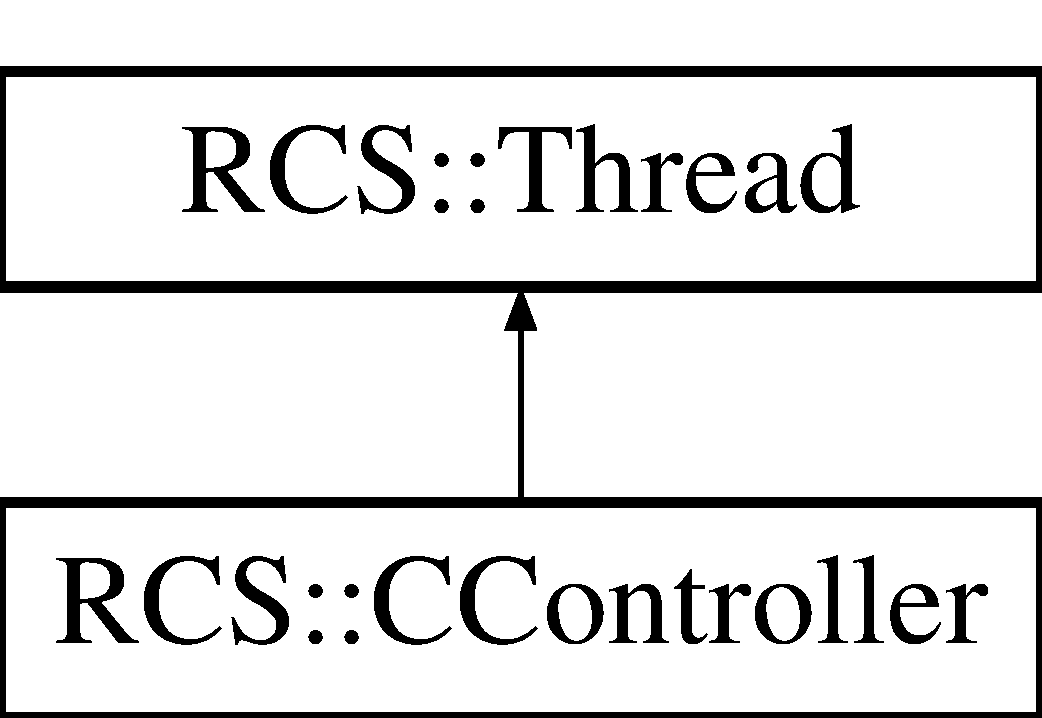
\includegraphics[height=2.000000cm]{structRCS_1_1CController}
\end{center}
\end{figure}
\subsection*{Public Types}
\begin{DoxyCompactItemize}
\item 
enum \hyperlink{structRCS_1_1CController_a50ede7cd9f47204828f0f7c740dc09b1}{Motion\-Planner\-Enum} \{ \\*
\hyperlink{structRCS_1_1CController_a50ede7cd9f47204828f0f7c740dc09b1ab00d7459e4ea68d1b1496592767bfc2f}{N\-O\-P\-L\-A\-N\-N\-E\-R} = 0, 
\hyperlink{structRCS_1_1CController_a50ede7cd9f47204828f0f7c740dc09b1a7904abb74c1bc4246b43b356be0704b5}{M\-O\-V\-E\-I\-T}, 
\hyperlink{structRCS_1_1CController_a50ede7cd9f47204828f0f7c740dc09b1a1506ec08ab80c752e9613c0d42e8accb}{D\-E\-S\-C\-A\-R\-T\-E\-S}, 
\hyperlink{structRCS_1_1CController_a50ede7cd9f47204828f0f7c740dc09b1aa492ff13d221452a2be124f579142e2f}{B\-A\-S\-I\-C}, 
\\*
\hyperlink{structRCS_1_1CController_a50ede7cd9f47204828f0f7c740dc09b1a2a75cf0f1dff3f261dcbf41639f0c2f9}{W\-A\-Y\-P\-O\-I\-N\-T}, 
\hyperlink{structRCS_1_1CController_a50ede7cd9f47204828f0f7c740dc09b1a063b2368ab3f63d194e7b4bc0182410e}{G\-O\-M\-O\-T\-I\-O\-N}
 \}
\item 
typedef std\-::list$<$ \hyperlink{structRCS_1_1CanonCmd}{R\-C\-S\-::\-Canon\-Cmd} $>$ \hyperlink{structRCS_1_1CController_aeaee07d36d39b56ecad1ce2443b5b4c0}{xml\-\_\-message\-\_\-list}
\end{DoxyCompactItemize}
\subsection*{Public Member Functions}
\begin{DoxyCompactItemize}
\item 
\hyperlink{structRCS_1_1CController_acf0744408b45b6d9f60cb44c9d64f1a8}{C\-Controller} (double cycletime)
\begin{DoxyCompactList}\small\item\em \hyperlink{structRCS_1_1CController}{C\-Controller} constructor that requires a cycle time for \hyperlink{namespaceRCS}{R\-C\-S} thread timing. \end{DoxyCompactList}\item 
\hyperlink{structRCS_1_1CController_a2bfe656f4d6a26d3dc4556ed8dab118a}{$\sim$\-C\-Controller} (void)
\item 
bool \hyperlink{structRCS_1_1CController_a7f04bc3e6f36033b2ea18bbac9c34a64}{Verify} ()
\begin{DoxyCompactList}\small\item\em Verifies that all the pointer references in the controller have been instantiated (i.\-e., not null). \end{DoxyCompactList}\item 
virtual int \hyperlink{structRCS_1_1CController_a0ca284e0879e57399044e6700630a526}{Action} ()
\begin{DoxyCompactList}\small\item\em Cyclic loop for the controller. Reads Crcl input mexsage queue, interprets into canon cmds if any, reads canon cmds queue, interprets into robot command messages. \end{DoxyCompactList}\item 
void \hyperlink{structRCS_1_1CController_a16ffe2c289a151554af8ed391774e215}{Setup} (ros\-::\-Node\-Handle \&nh, std\-::string prefix)
\begin{DoxyCompactList}\small\item\em Setup routine for the controller.. \end{DoxyCompactList}\item 
std\-::string \hyperlink{structRCS_1_1CController_aa7c4b106c4fb8064d896ccad7ce25b46}{Dump} (std\-::string separator=\char`\"{},\char`\"{})
\begin{DoxyCompactList}\small\item\em Creates a comma separated string of current state of robot. (Can use other separator). \end{DoxyCompactList}\item 
std\-::string \hyperlink{structRCS_1_1CController_aaf2b0286ce10f78e5eee44e3613e588e}{Dump\-Header} (std\-::string separator=\char`\"{},\char`\"{})
\begin{DoxyCompactList}\small\item\em Creates a header line containing names of comma separated string fields that describes the current state of robot. (Can use other separator). \end{DoxyCompactList}\item 
\hyperlink{structRCS_1_1CController_abb822466798247a45d3206ecae9c36fc}{V\-A\-R} (\hyperlink{classKinematics}{Kinematics}, boost\-::shared\-\_\-ptr$<$ \hyperlink{classIKinematics}{I\-Kinematics} $>$)
\item 
\hyperlink{structRCS_1_1CController_abe34674042d0b1b983a3e4117310f66c}{V\-A\-R} (Joint\-Writer, boost\-::shared\-\_\-ptr$<$ \hyperlink{classCJointWriter}{C\-Joint\-Writer} $>$)
\item 
\hyperlink{structRCS_1_1CController_a8d733f4562e66f359ca58c2d9d2d73fe}{V\-A\-R} (b\-Simulation, bool) V\-A\-R(gripper\-Pose
\item 
\hyperlink{structRCS_1_1CController_ad9ff9933db2721ba89e532fc57a871f8}{V\-A\-R} (inv\-Gripper\-Pose, \hyperlink{namespaceRCS_aa07e45d8a50e30064283d2b38087f999}{R\-C\-S\-::\-Pose})
\item 
\hyperlink{structRCS_1_1CController_adba057520bba1b50d7fd344f67b1705b}{V\-A\-R} (base\-Pose, \hyperlink{namespaceRCS_aa07e45d8a50e30064283d2b38087f999}{R\-C\-S\-::\-Pose})
\item 
\hyperlink{structRCS_1_1CController_a2d522e82da5f5d2296ea97e4d22b858d}{V\-A\-R} (inv\-Base\-Pose, \hyperlink{namespaceRCS_aa07e45d8a50e30064283d2b38087f999}{R\-C\-S\-::\-Pose})
\item 
void \hyperlink{structRCS_1_1CController_a10aa8d4a96d6dfe4c0da398f2fa5ba0e}{Cmd\-Callback} (const nistcrcl\-::\-Crcl\-Command\-Msg\-::\-Const\-Ptr \&cmdmsg)
\item 
void \hyperlink{structRCS_1_1CController_aaf7dfe624a26a906d715b73a337ea927}{Motion\-Logging} ()
\item 
void \hyperlink{structRCS_1_1CController_a02cf331e363cf90ddd6b4e0e8532b73f}{Publish\-Crcl\-Status} ()
\item 
void \hyperlink{structRCS_1_1CController_a2733d3cf36b11a6b257e04a969e03abf}{Set\-Kinematics} (boost\-::shared\-\_\-ptr$<$ \hyperlink{classIKinematics}{I\-Kinematics} $>$ k)
\begin{DoxyCompactList}\small\item\em Routine to set the kinematics reference pointer. Uses the interface class \hyperlink{classIKinematics}{I\-Kinematics}, but can have any implementation instance. \end{DoxyCompactList}\item 
\hyperlink{structRCS_1_1CController_a5113cb8a1cfaf75459e8a2b13802312e}{N\-V\-A\-R} (New\-C\-C, \hyperlink{structRCS_1_1CanonCmd}{R\-C\-S\-::\-Canon\-Cmd}, \-\_\-newcc)
\item 
\hyperlink{structRCS_1_1CController_a1b85d1d02e33dbfe25173575f17d4498}{N\-V\-A\-R} (Last\-C\-C, \hyperlink{structRCS_1_1CanonCmd}{R\-C\-S\-::\-Canon\-Cmd}, \-\_\-lastcc)
\item 
\hyperlink{structRCS_1_1CanonCmd}{R\-C\-S\-::\-Canon\-Cmd} \hyperlink{structRCS_1_1CController_af150048fb1660e68d9f5ec1043494ea9}{Get\-Last\-Robot\-Command} ()
\item 
\hyperlink{RCS_8h_aa4adb93a26caa4dacba9c9614e283245}{Joint\-State} \hyperlink{structRCS_1_1CController_a7334e3abcc69cc6e3a9f82e59c682551}{Get\-Last\-Joint\-State} ()
\begin{DoxyCompactList}\small\item\em Get the last joint state, if no motion, last actual joint reading, else last joints on robot motion queue. \end{DoxyCompactList}\item 
\hyperlink{namespaceRCS_aa07e45d8a50e30064283d2b38087f999}{R\-C\-S\-::\-Pose} \hyperlink{structRCS_1_1CController_ae7230e4ecd977fb1519b13b2ed696897}{Get\-Last\-Commanded\-Pose} ()
\begin{DoxyCompactList}\small\item\em Get the last commanded , if no motion, use last actual joint reading to compute F\-K, else use last joints on robot motion queue to compute F\-K. \end{DoxyCompactList}\end{DoxyCompactItemize}
\subsection*{Public Attributes}
\begin{DoxyCompactItemize}
\item 
\hyperlink{structRCS_1_1CanonWorldModel}{R\-C\-S\-::\-Canon\-World\-Model} \hyperlink{structRCS_1_1CController_a82e9cc233cd25554964efe8a9008e0b2}{status}
\item 
\hyperlink{structRCS_1_1CanonWorldModel}{R\-C\-S\-::\-Canon\-World\-Model} \hyperlink{structRCS_1_1CController_af76ac9412dbefbaebc970d62f88a40fa}{laststatus}
\item 
\hyperlink{classRCS_1_1CMessageQueue}{R\-C\-S\-::\-C\-Message\-Queue}\\*
$<$ nistcrcl\-::\-Crcl\-Command\-Msg $>$ \hyperlink{structRCS_1_1CController_a90aefbaf6e37b3902951d48365e6c6da}{crclcmds}
\item 
std\-::list$<$ \hyperlink{structRCS_1_1CanonCmd}{R\-C\-S\-::\-Canon\-Cmd} $>$ \hyperlink{structRCS_1_1CController_a1801fcf66f2d28f00bf91f65634ae4df}{donecmds}
\item 
\hyperlink{classRCS_1_1CMessageQueue}{R\-C\-S\-::\-C\-Message\-Queue}$<$ \hyperlink{structRCS_1_1CanonCmd}{R\-C\-S\-::\-Canon\-Cmd} $>$ \hyperlink{structRCS_1_1CController_a6704a1f1b72409d251222738086b21c1}{robotcmds}
\item 
ros\-::\-Publisher \hyperlink{structRCS_1_1CController_a059fc88d65194dc7a78737b80cd88628}{crcl\-\_\-status}
\item 
ros\-::\-Subscriber \hyperlink{structRCS_1_1CController_a68d8609778f84a1f4648270d57bcbf8a}{crcl\-\_\-cmd}
\item 
ros\-::\-Publisher \hyperlink{structRCS_1_1CController_a53d259a8d8c319b8f118f37eb010ff5e}{rviz\-\_\-jntcmd}
\item 
ros\-::\-Node\-Handle $\ast$ \hyperlink{structRCS_1_1CController_aded52f628534d0ebf9558b49b9314fef}{\-\_\-nh}
\item 
\hyperlink{classGripperInterface}{Gripper\-Interface} \hyperlink{structRCS_1_1CController_a99ad3b40383ec1a48e55a56f1a91771f}{gripper}
\item 
boost\-::shared\-\_\-ptr\\*
$<$ \hyperlink{classRCS_1_1IRCSInterpreter}{I\-R\-C\-S\-Interpreter} $>$ \hyperlink{structRCS_1_1CController_ae5d5ab2480680d7db766f7810232b696}{\-\_\-interpreter}
\item 
\hyperlink{structRCS_1_1CController_a50ede7cd9f47204828f0f7c740dc09b1}{Motion\-Planner\-Enum} \hyperlink{structRCS_1_1CController_a4174fd5467045e780fe53bde42e70735}{e\-Cartesian\-Motion\-Planner}
\item 
\hyperlink{structRCS_1_1CController_a50ede7cd9f47204828f0f7c740dc09b1}{Motion\-Planner\-Enum} \hyperlink{structRCS_1_1CController_ad788d0def2101be74b680394bcbc78e7}{e\-Joint\-Motion\-Planner}
\end{DoxyCompactItemize}
\subsection*{Additional Inherited Members}


\subsection{Detailed Description}
The \hyperlink{structRCS_1_1CController}{C\-Controller} provides a collection for all the relevant controller pieces. The \hyperlink{structRCS_1_1CController}{C\-Controller} is the main controller class to collect all the references/pointers to instances in the project. A global instance of this class, called \char`\"{}\-Controller\char`\"{}, is created and is used throughout the code to reference various instances of control objects (e.\-g., kinematics, joint writer, joint reader, etc.) 

\subsection{Member Typedef Documentation}
\hypertarget{structRCS_1_1CController_aeaee07d36d39b56ecad1ce2443b5b4c0}{\index{R\-C\-S\-::\-C\-Controller@{R\-C\-S\-::\-C\-Controller}!xml\-\_\-message\-\_\-list@{xml\-\_\-message\-\_\-list}}
\index{xml\-\_\-message\-\_\-list@{xml\-\_\-message\-\_\-list}!RCS::CController@{R\-C\-S\-::\-C\-Controller}}
\subsubsection[{xml\-\_\-message\-\_\-list}]{\setlength{\rightskip}{0pt plus 5cm}typedef std\-::list$<${\bf R\-C\-S\-::\-Canon\-Cmd}$>$ {\bf R\-C\-S\-::\-C\-Controller\-::xml\-\_\-message\-\_\-list}}}\label{structRCS_1_1CController_aeaee07d36d39b56ecad1ce2443b5b4c0}


\subsection{Member Enumeration Documentation}
\hypertarget{structRCS_1_1CController_a50ede7cd9f47204828f0f7c740dc09b1}{\index{R\-C\-S\-::\-C\-Controller@{R\-C\-S\-::\-C\-Controller}!Motion\-Planner\-Enum@{Motion\-Planner\-Enum}}
\index{Motion\-Planner\-Enum@{Motion\-Planner\-Enum}!RCS::CController@{R\-C\-S\-::\-C\-Controller}}
\subsubsection[{Motion\-Planner\-Enum}]{\setlength{\rightskip}{0pt plus 5cm}enum {\bf R\-C\-S\-::\-C\-Controller\-::\-Motion\-Planner\-Enum}}}\label{structRCS_1_1CController_a50ede7cd9f47204828f0f7c740dc09b1}
\begin{Desc}
\item[Enumerator]\par
\begin{description}
\index{N\-O\-P\-L\-A\-N\-N\-E\-R@{N\-O\-P\-L\-A\-N\-N\-E\-R}!R\-C\-S\-::\-C\-Controller@{R\-C\-S\-::\-C\-Controller}}\index{R\-C\-S\-::\-C\-Controller@{R\-C\-S\-::\-C\-Controller}!N\-O\-P\-L\-A\-N\-N\-E\-R@{N\-O\-P\-L\-A\-N\-N\-E\-R}}\item[{\em 
\hypertarget{structRCS_1_1CController_a50ede7cd9f47204828f0f7c740dc09b1ab00d7459e4ea68d1b1496592767bfc2f}{N\-O\-P\-L\-A\-N\-N\-E\-R}\label{structRCS_1_1CController_a50ede7cd9f47204828f0f7c740dc09b1ab00d7459e4ea68d1b1496592767bfc2f}
}]\index{M\-O\-V\-E\-I\-T@{M\-O\-V\-E\-I\-T}!R\-C\-S\-::\-C\-Controller@{R\-C\-S\-::\-C\-Controller}}\index{R\-C\-S\-::\-C\-Controller@{R\-C\-S\-::\-C\-Controller}!M\-O\-V\-E\-I\-T@{M\-O\-V\-E\-I\-T}}\item[{\em 
\hypertarget{structRCS_1_1CController_a50ede7cd9f47204828f0f7c740dc09b1a7904abb74c1bc4246b43b356be0704b5}{M\-O\-V\-E\-I\-T}\label{structRCS_1_1CController_a50ede7cd9f47204828f0f7c740dc09b1a7904abb74c1bc4246b43b356be0704b5}
}]\index{D\-E\-S\-C\-A\-R\-T\-E\-S@{D\-E\-S\-C\-A\-R\-T\-E\-S}!R\-C\-S\-::\-C\-Controller@{R\-C\-S\-::\-C\-Controller}}\index{R\-C\-S\-::\-C\-Controller@{R\-C\-S\-::\-C\-Controller}!D\-E\-S\-C\-A\-R\-T\-E\-S@{D\-E\-S\-C\-A\-R\-T\-E\-S}}\item[{\em 
\hypertarget{structRCS_1_1CController_a50ede7cd9f47204828f0f7c740dc09b1a1506ec08ab80c752e9613c0d42e8accb}{D\-E\-S\-C\-A\-R\-T\-E\-S}\label{structRCS_1_1CController_a50ede7cd9f47204828f0f7c740dc09b1a1506ec08ab80c752e9613c0d42e8accb}
}]\index{B\-A\-S\-I\-C@{B\-A\-S\-I\-C}!R\-C\-S\-::\-C\-Controller@{R\-C\-S\-::\-C\-Controller}}\index{R\-C\-S\-::\-C\-Controller@{R\-C\-S\-::\-C\-Controller}!B\-A\-S\-I\-C@{B\-A\-S\-I\-C}}\item[{\em 
\hypertarget{structRCS_1_1CController_a50ede7cd9f47204828f0f7c740dc09b1aa492ff13d221452a2be124f579142e2f}{B\-A\-S\-I\-C}\label{structRCS_1_1CController_a50ede7cd9f47204828f0f7c740dc09b1aa492ff13d221452a2be124f579142e2f}
}]\index{W\-A\-Y\-P\-O\-I\-N\-T@{W\-A\-Y\-P\-O\-I\-N\-T}!R\-C\-S\-::\-C\-Controller@{R\-C\-S\-::\-C\-Controller}}\index{R\-C\-S\-::\-C\-Controller@{R\-C\-S\-::\-C\-Controller}!W\-A\-Y\-P\-O\-I\-N\-T@{W\-A\-Y\-P\-O\-I\-N\-T}}\item[{\em 
\hypertarget{structRCS_1_1CController_a50ede7cd9f47204828f0f7c740dc09b1a2a75cf0f1dff3f261dcbf41639f0c2f9}{W\-A\-Y\-P\-O\-I\-N\-T}\label{structRCS_1_1CController_a50ede7cd9f47204828f0f7c740dc09b1a2a75cf0f1dff3f261dcbf41639f0c2f9}
}]\index{G\-O\-M\-O\-T\-I\-O\-N@{G\-O\-M\-O\-T\-I\-O\-N}!R\-C\-S\-::\-C\-Controller@{R\-C\-S\-::\-C\-Controller}}\index{R\-C\-S\-::\-C\-Controller@{R\-C\-S\-::\-C\-Controller}!G\-O\-M\-O\-T\-I\-O\-N@{G\-O\-M\-O\-T\-I\-O\-N}}\item[{\em 
\hypertarget{structRCS_1_1CController_a50ede7cd9f47204828f0f7c740dc09b1a063b2368ab3f63d194e7b4bc0182410e}{G\-O\-M\-O\-T\-I\-O\-N}\label{structRCS_1_1CController_a50ede7cd9f47204828f0f7c740dc09b1a063b2368ab3f63d194e7b4bc0182410e}
}]\end{description}
\end{Desc}


\subsection{Constructor \& Destructor Documentation}
\hypertarget{structRCS_1_1CController_acf0744408b45b6d9f60cb44c9d64f1a8}{\index{R\-C\-S\-::\-C\-Controller@{R\-C\-S\-::\-C\-Controller}!C\-Controller@{C\-Controller}}
\index{C\-Controller@{C\-Controller}!RCS::CController@{R\-C\-S\-::\-C\-Controller}}
\subsubsection[{C\-Controller}]{\setlength{\rightskip}{0pt plus 5cm}R\-C\-S\-::\-C\-Controller\-::\-C\-Controller (
\begin{DoxyParamCaption}
\item[{double}]{cycletime}
\end{DoxyParamCaption}
)}}\label{structRCS_1_1CController_acf0744408b45b6d9f60cb44c9d64f1a8}


\hyperlink{structRCS_1_1CController}{C\-Controller} constructor that requires a cycle time for \hyperlink{namespaceRCS}{R\-C\-S} thread timing. 


\begin{DoxyParams}{Parameters}
{\em cycletime} & in seconds. \\
\hline
\end{DoxyParams}
\hypertarget{structRCS_1_1CController_a2bfe656f4d6a26d3dc4556ed8dab118a}{\index{R\-C\-S\-::\-C\-Controller@{R\-C\-S\-::\-C\-Controller}!$\sim$\-C\-Controller@{$\sim$\-C\-Controller}}
\index{$\sim$\-C\-Controller@{$\sim$\-C\-Controller}!RCS::CController@{R\-C\-S\-::\-C\-Controller}}
\subsubsection[{$\sim$\-C\-Controller}]{\setlength{\rightskip}{0pt plus 5cm}R\-C\-S\-::\-C\-Controller\-::$\sim$\-C\-Controller (
\begin{DoxyParamCaption}
\item[{void}]{}
\end{DoxyParamCaption}
)}}\label{structRCS_1_1CController_a2bfe656f4d6a26d3dc4556ed8dab118a}


\subsection{Member Function Documentation}
\hypertarget{structRCS_1_1CController_a0ca284e0879e57399044e6700630a526}{\index{R\-C\-S\-::\-C\-Controller@{R\-C\-S\-::\-C\-Controller}!Action@{Action}}
\index{Action@{Action}!RCS::CController@{R\-C\-S\-::\-C\-Controller}}
\subsubsection[{Action}]{\setlength{\rightskip}{0pt plus 5cm}int R\-C\-S\-::\-C\-Controller\-::\-Action (
\begin{DoxyParamCaption}
{}
\end{DoxyParamCaption}
)\hspace{0.3cm}{\ttfamily [virtual]}}}\label{structRCS_1_1CController_a0ca284e0879e57399044e6700630a526}


Cyclic loop for the controller. Reads Crcl input mexsage queue, interprets into canon cmds if any, reads canon cmds queue, interprets into robot command messages. 

std\-\_\-msgs/\-Header headerposition uint8 crclcommandnum uint8 crclstatusnum uint8 crclcommandstatus \subparagraph*{}

uint8 done=0 uint8 error=1 uint8 working=2 \subparagraph*{}

geometry\-\_\-msgs/\-Pose statuspose sensor\-\_\-msgs/\-Joint\-State statusjoints float64 eepercent $<$ current robot pose 

Reimplemented from \hyperlink{classRCS_1_1Thread_a78aec7128f4fbf5d6859ceb09f9f9ae1}{R\-C\-S\-::\-Thread}.

\hypertarget{structRCS_1_1CController_a10aa8d4a96d6dfe4c0da398f2fa5ba0e}{\index{R\-C\-S\-::\-C\-Controller@{R\-C\-S\-::\-C\-Controller}!Cmd\-Callback@{Cmd\-Callback}}
\index{Cmd\-Callback@{Cmd\-Callback}!RCS::CController@{R\-C\-S\-::\-C\-Controller}}
\subsubsection[{Cmd\-Callback}]{\setlength{\rightskip}{0pt plus 5cm}void R\-C\-S\-::\-C\-Controller\-::\-Cmd\-Callback (
\begin{DoxyParamCaption}
\item[{const nistcrcl\-::\-Crcl\-Command\-Msg\-::\-Const\-Ptr \&}]{cmdmsg}
\end{DoxyParamCaption}
)}}\label{structRCS_1_1CController_a10aa8d4a96d6dfe4c0da398f2fa5ba0e}
\hypertarget{structRCS_1_1CController_aa7c4b106c4fb8064d896ccad7ce25b46}{\index{R\-C\-S\-::\-C\-Controller@{R\-C\-S\-::\-C\-Controller}!Dump@{Dump}}
\index{Dump@{Dump}!RCS::CController@{R\-C\-S\-::\-C\-Controller}}
\subsubsection[{Dump}]{\setlength{\rightskip}{0pt plus 5cm}std\-::string R\-C\-S\-::\-C\-Controller\-::\-Dump (
\begin{DoxyParamCaption}
\item[{std\-::string}]{separator = {\ttfamily \char`\"{},\char`\"{}}}
\end{DoxyParamCaption}
)}}\label{structRCS_1_1CController_aa7c4b106c4fb8064d896ccad7ce25b46}


Creates a comma separated string of current state of robot. (Can use other separator). 

\hypertarget{structRCS_1_1CController_aaf2b0286ce10f78e5eee44e3613e588e}{\index{R\-C\-S\-::\-C\-Controller@{R\-C\-S\-::\-C\-Controller}!Dump\-Header@{Dump\-Header}}
\index{Dump\-Header@{Dump\-Header}!RCS::CController@{R\-C\-S\-::\-C\-Controller}}
\subsubsection[{Dump\-Header}]{\setlength{\rightskip}{0pt plus 5cm}std\-::string R\-C\-S\-::\-C\-Controller\-::\-Dump\-Header (
\begin{DoxyParamCaption}
\item[{std\-::string}]{separator = {\ttfamily \char`\"{},\char`\"{}}}
\end{DoxyParamCaption}
)}}\label{structRCS_1_1CController_aaf2b0286ce10f78e5eee44e3613e588e}


Creates a header line containing names of comma separated string fields that describes the current state of robot. (Can use other separator). 

\hypertarget{structRCS_1_1CController_ae7230e4ecd977fb1519b13b2ed696897}{\index{R\-C\-S\-::\-C\-Controller@{R\-C\-S\-::\-C\-Controller}!Get\-Last\-Commanded\-Pose@{Get\-Last\-Commanded\-Pose}}
\index{Get\-Last\-Commanded\-Pose@{Get\-Last\-Commanded\-Pose}!RCS::CController@{R\-C\-S\-::\-C\-Controller}}
\subsubsection[{Get\-Last\-Commanded\-Pose}]{\setlength{\rightskip}{0pt plus 5cm}{\bf R\-C\-S\-::\-Pose} R\-C\-S\-::\-C\-Controller\-::\-Get\-Last\-Commanded\-Pose (
\begin{DoxyParamCaption}
{}
\end{DoxyParamCaption}
)}}\label{structRCS_1_1CController_ae7230e4ecd977fb1519b13b2ed696897}


Get the last commanded , if no motion, use last actual joint reading to compute F\-K, else use last joints on robot motion queue to compute F\-K. 

\hypertarget{structRCS_1_1CController_a7334e3abcc69cc6e3a9f82e59c682551}{\index{R\-C\-S\-::\-C\-Controller@{R\-C\-S\-::\-C\-Controller}!Get\-Last\-Joint\-State@{Get\-Last\-Joint\-State}}
\index{Get\-Last\-Joint\-State@{Get\-Last\-Joint\-State}!RCS::CController@{R\-C\-S\-::\-C\-Controller}}
\subsubsection[{Get\-Last\-Joint\-State}]{\setlength{\rightskip}{0pt plus 5cm}{\bf Joint\-State} R\-C\-S\-::\-C\-Controller\-::\-Get\-Last\-Joint\-State (
\begin{DoxyParamCaption}
{}
\end{DoxyParamCaption}
)}}\label{structRCS_1_1CController_a7334e3abcc69cc6e3a9f82e59c682551}


Get the last joint state, if no motion, last actual joint reading, else last joints on robot motion queue. 

\hypertarget{structRCS_1_1CController_af150048fb1660e68d9f5ec1043494ea9}{\index{R\-C\-S\-::\-C\-Controller@{R\-C\-S\-::\-C\-Controller}!Get\-Last\-Robot\-Command@{Get\-Last\-Robot\-Command}}
\index{Get\-Last\-Robot\-Command@{Get\-Last\-Robot\-Command}!RCS::CController@{R\-C\-S\-::\-C\-Controller}}
\subsubsection[{Get\-Last\-Robot\-Command}]{\setlength{\rightskip}{0pt plus 5cm}{\bf R\-C\-S\-::\-Canon\-Cmd} R\-C\-S\-::\-C\-Controller\-::\-Get\-Last\-Robot\-Command (
\begin{DoxyParamCaption}
{}
\end{DoxyParamCaption}
)}}\label{structRCS_1_1CController_af150048fb1660e68d9f5ec1043494ea9}
\hypertarget{structRCS_1_1CController_aaf7dfe624a26a906d715b73a337ea927}{\index{R\-C\-S\-::\-C\-Controller@{R\-C\-S\-::\-C\-Controller}!Motion\-Logging@{Motion\-Logging}}
\index{Motion\-Logging@{Motion\-Logging}!RCS::CController@{R\-C\-S\-::\-C\-Controller}}
\subsubsection[{Motion\-Logging}]{\setlength{\rightskip}{0pt plus 5cm}void R\-C\-S\-::\-C\-Controller\-::\-Motion\-Logging (
\begin{DoxyParamCaption}
{}
\end{DoxyParamCaption}
)}}\label{structRCS_1_1CController_aaf7dfe624a26a906d715b73a337ea927}
\hypertarget{structRCS_1_1CController_a5113cb8a1cfaf75459e8a2b13802312e}{\index{R\-C\-S\-::\-C\-Controller@{R\-C\-S\-::\-C\-Controller}!N\-V\-A\-R@{N\-V\-A\-R}}
\index{N\-V\-A\-R@{N\-V\-A\-R}!RCS::CController@{R\-C\-S\-::\-C\-Controller}}
\subsubsection[{N\-V\-A\-R}]{\setlength{\rightskip}{0pt plus 5cm}R\-C\-S\-::\-C\-Controller\-::\-N\-V\-A\-R (
\begin{DoxyParamCaption}
\item[{New\-C\-C}]{, }
\item[{{\bf R\-C\-S\-::\-Canon\-Cmd}}]{, }
\item[{\-\_\-newcc}]{}
\end{DoxyParamCaption}
)}}\label{structRCS_1_1CController_a5113cb8a1cfaf75459e8a2b13802312e}
last canon command interpreted \hypertarget{structRCS_1_1CController_a1b85d1d02e33dbfe25173575f17d4498}{\index{R\-C\-S\-::\-C\-Controller@{R\-C\-S\-::\-C\-Controller}!N\-V\-A\-R@{N\-V\-A\-R}}
\index{N\-V\-A\-R@{N\-V\-A\-R}!RCS::CController@{R\-C\-S\-::\-C\-Controller}}
\subsubsection[{N\-V\-A\-R}]{\setlength{\rightskip}{0pt plus 5cm}R\-C\-S\-::\-C\-Controller\-::\-N\-V\-A\-R (
\begin{DoxyParamCaption}
\item[{Last\-C\-C}]{, }
\item[{{\bf R\-C\-S\-::\-Canon\-Cmd}}]{, }
\item[{\-\_\-lastcc}]{}
\end{DoxyParamCaption}
)}}\label{structRCS_1_1CController_a1b85d1d02e33dbfe25173575f17d4498}
\hypertarget{structRCS_1_1CController_a02cf331e363cf90ddd6b4e0e8532b73f}{\index{R\-C\-S\-::\-C\-Controller@{R\-C\-S\-::\-C\-Controller}!Publish\-Crcl\-Status@{Publish\-Crcl\-Status}}
\index{Publish\-Crcl\-Status@{Publish\-Crcl\-Status}!RCS::CController@{R\-C\-S\-::\-C\-Controller}}
\subsubsection[{Publish\-Crcl\-Status}]{\setlength{\rightskip}{0pt plus 5cm}void R\-C\-S\-::\-C\-Controller\-::\-Publish\-Crcl\-Status (
\begin{DoxyParamCaption}
{}
\end{DoxyParamCaption}
)}}\label{structRCS_1_1CController_a02cf331e363cf90ddd6b4e0e8532b73f}
$<$ current robot pose \hypertarget{structRCS_1_1CController_a2733d3cf36b11a6b257e04a969e03abf}{\index{R\-C\-S\-::\-C\-Controller@{R\-C\-S\-::\-C\-Controller}!Set\-Kinematics@{Set\-Kinematics}}
\index{Set\-Kinematics@{Set\-Kinematics}!RCS::CController@{R\-C\-S\-::\-C\-Controller}}
\subsubsection[{Set\-Kinematics}]{\setlength{\rightskip}{0pt plus 5cm}void R\-C\-S\-::\-C\-Controller\-::\-Set\-Kinematics (
\begin{DoxyParamCaption}
\item[{boost\-::shared\-\_\-ptr$<$ {\bf I\-Kinematics} $>$}]{k}
\end{DoxyParamCaption}
)\hspace{0.3cm}{\ttfamily [inline]}}}\label{structRCS_1_1CController_a2733d3cf36b11a6b257e04a969e03abf}


Routine to set the kinematics reference pointer. Uses the interface class \hyperlink{classIKinematics}{I\-Kinematics}, but can have any implementation instance. 

\hypertarget{structRCS_1_1CController_a16ffe2c289a151554af8ed391774e215}{\index{R\-C\-S\-::\-C\-Controller@{R\-C\-S\-::\-C\-Controller}!Setup@{Setup}}
\index{Setup@{Setup}!RCS::CController@{R\-C\-S\-::\-C\-Controller}}
\subsubsection[{Setup}]{\setlength{\rightskip}{0pt plus 5cm}void R\-C\-S\-::\-C\-Controller\-::\-Setup (
\begin{DoxyParamCaption}
\item[{ros\-::\-Node\-Handle \&}]{nh, }
\item[{std\-::string}]{prefix}
\end{DoxyParamCaption}
)}}\label{structRCS_1_1CController_a16ffe2c289a151554af8ed391774e215}


Setup routine for the controller.. 

\hypertarget{structRCS_1_1CController_abb822466798247a45d3206ecae9c36fc}{\index{R\-C\-S\-::\-C\-Controller@{R\-C\-S\-::\-C\-Controller}!V\-A\-R@{V\-A\-R}}
\index{V\-A\-R@{V\-A\-R}!RCS::CController@{R\-C\-S\-::\-C\-Controller}}
\subsubsection[{V\-A\-R}]{\setlength{\rightskip}{0pt plus 5cm}R\-C\-S\-::\-C\-Controller\-::\-V\-A\-R (
\begin{DoxyParamCaption}
\item[{{\bf Kinematics}}]{, }
\item[{boost\-::shared\-\_\-ptr$<$ {\bf I\-Kinematics} $>$}]{}
\end{DoxyParamCaption}
)}}\label{structRCS_1_1CController_abb822466798247a45d3206ecae9c36fc}
\hypertarget{structRCS_1_1CController_abe34674042d0b1b983a3e4117310f66c}{\index{R\-C\-S\-::\-C\-Controller@{R\-C\-S\-::\-C\-Controller}!V\-A\-R@{V\-A\-R}}
\index{V\-A\-R@{V\-A\-R}!RCS::CController@{R\-C\-S\-::\-C\-Controller}}
\subsubsection[{V\-A\-R}]{\setlength{\rightskip}{0pt plus 5cm}R\-C\-S\-::\-C\-Controller\-::\-V\-A\-R (
\begin{DoxyParamCaption}
\item[{Joint\-Writer}]{, }
\item[{boost\-::shared\-\_\-ptr$<$ {\bf C\-Joint\-Writer} $>$}]{}
\end{DoxyParamCaption}
)}}\label{structRCS_1_1CController_abe34674042d0b1b983a3e4117310f66c}
\hypertarget{structRCS_1_1CController_a8d733f4562e66f359ca58c2d9d2d73fe}{\index{R\-C\-S\-::\-C\-Controller@{R\-C\-S\-::\-C\-Controller}!V\-A\-R@{V\-A\-R}}
\index{V\-A\-R@{V\-A\-R}!RCS::CController@{R\-C\-S\-::\-C\-Controller}}
\subsubsection[{V\-A\-R}]{\setlength{\rightskip}{0pt plus 5cm}R\-C\-S\-::\-C\-Controller\-::\-V\-A\-R (
\begin{DoxyParamCaption}
\item[{b\-Simulation}]{, }
\item[{bool}]{}
\end{DoxyParamCaption}
)}}\label{structRCS_1_1CController_a8d733f4562e66f359ca58c2d9d2d73fe}
\hypertarget{structRCS_1_1CController_ad9ff9933db2721ba89e532fc57a871f8}{\index{R\-C\-S\-::\-C\-Controller@{R\-C\-S\-::\-C\-Controller}!V\-A\-R@{V\-A\-R}}
\index{V\-A\-R@{V\-A\-R}!RCS::CController@{R\-C\-S\-::\-C\-Controller}}
\subsubsection[{V\-A\-R}]{\setlength{\rightskip}{0pt plus 5cm}R\-C\-S\-::\-C\-Controller\-::\-V\-A\-R (
\begin{DoxyParamCaption}
\item[{inv\-Gripper\-Pose}]{, }
\item[{{\bf R\-C\-S\-::\-Pose}}]{}
\end{DoxyParamCaption}
)}}\label{structRCS_1_1CController_ad9ff9933db2721ba89e532fc57a871f8}
\hypertarget{structRCS_1_1CController_adba057520bba1b50d7fd344f67b1705b}{\index{R\-C\-S\-::\-C\-Controller@{R\-C\-S\-::\-C\-Controller}!V\-A\-R@{V\-A\-R}}
\index{V\-A\-R@{V\-A\-R}!RCS::CController@{R\-C\-S\-::\-C\-Controller}}
\subsubsection[{V\-A\-R}]{\setlength{\rightskip}{0pt plus 5cm}R\-C\-S\-::\-C\-Controller\-::\-V\-A\-R (
\begin{DoxyParamCaption}
\item[{base\-Pose}]{, }
\item[{{\bf R\-C\-S\-::\-Pose}}]{}
\end{DoxyParamCaption}
)}}\label{structRCS_1_1CController_adba057520bba1b50d7fd344f67b1705b}
\hypertarget{structRCS_1_1CController_a2d522e82da5f5d2296ea97e4d22b858d}{\index{R\-C\-S\-::\-C\-Controller@{R\-C\-S\-::\-C\-Controller}!V\-A\-R@{V\-A\-R}}
\index{V\-A\-R@{V\-A\-R}!RCS::CController@{R\-C\-S\-::\-C\-Controller}}
\subsubsection[{V\-A\-R}]{\setlength{\rightskip}{0pt plus 5cm}R\-C\-S\-::\-C\-Controller\-::\-V\-A\-R (
\begin{DoxyParamCaption}
\item[{inv\-Base\-Pose}]{, }
\item[{{\bf R\-C\-S\-::\-Pose}}]{}
\end{DoxyParamCaption}
)}}\label{structRCS_1_1CController_a2d522e82da5f5d2296ea97e4d22b858d}
\hypertarget{structRCS_1_1CController_a7f04bc3e6f36033b2ea18bbac9c34a64}{\index{R\-C\-S\-::\-C\-Controller@{R\-C\-S\-::\-C\-Controller}!Verify@{Verify}}
\index{Verify@{Verify}!RCS::CController@{R\-C\-S\-::\-C\-Controller}}
\subsubsection[{Verify}]{\setlength{\rightskip}{0pt plus 5cm}bool R\-C\-S\-::\-C\-Controller\-::\-Verify (
\begin{DoxyParamCaption}
{}
\end{DoxyParamCaption}
)}}\label{structRCS_1_1CController_a7f04bc3e6f36033b2ea18bbac9c34a64}


Verifies that all the pointer references in the controller have been instantiated (i.\-e., not null). 



\subsection{Member Data Documentation}
\hypertarget{structRCS_1_1CController_ae5d5ab2480680d7db766f7810232b696}{\index{R\-C\-S\-::\-C\-Controller@{R\-C\-S\-::\-C\-Controller}!\-\_\-interpreter@{\-\_\-interpreter}}
\index{\-\_\-interpreter@{\-\_\-interpreter}!RCS::CController@{R\-C\-S\-::\-C\-Controller}}
\subsubsection[{\-\_\-interpreter}]{\setlength{\rightskip}{0pt plus 5cm}boost\-::shared\-\_\-ptr$<${\bf I\-R\-C\-S\-Interpreter}$>$ R\-C\-S\-::\-C\-Controller\-::\-\_\-interpreter}}\label{structRCS_1_1CController_ae5d5ab2480680d7db766f7810232b696}
interprets canon commands into robot commands current new canon command to interpret \hypertarget{structRCS_1_1CController_aded52f628534d0ebf9558b49b9314fef}{\index{R\-C\-S\-::\-C\-Controller@{R\-C\-S\-::\-C\-Controller}!\-\_\-nh@{\-\_\-nh}}
\index{\-\_\-nh@{\-\_\-nh}!RCS::CController@{R\-C\-S\-::\-C\-Controller}}
\subsubsection[{\-\_\-nh}]{\setlength{\rightskip}{0pt plus 5cm}ros\-::\-Node\-Handle$\ast$ R\-C\-S\-::\-C\-Controller\-::\-\_\-nh}}\label{structRCS_1_1CController_aded52f628534d0ebf9558b49b9314fef}
\hypertarget{structRCS_1_1CController_a68d8609778f84a1f4648270d57bcbf8a}{\index{R\-C\-S\-::\-C\-Controller@{R\-C\-S\-::\-C\-Controller}!crcl\-\_\-cmd@{crcl\-\_\-cmd}}
\index{crcl\-\_\-cmd@{crcl\-\_\-cmd}!RCS::CController@{R\-C\-S\-::\-C\-Controller}}
\subsubsection[{crcl\-\_\-cmd}]{\setlength{\rightskip}{0pt plus 5cm}ros\-::\-Subscriber R\-C\-S\-::\-C\-Controller\-::crcl\-\_\-cmd}}\label{structRCS_1_1CController_a68d8609778f84a1f4648270d57bcbf8a}
ros subscriber information used for crcl command updates \hypertarget{structRCS_1_1CController_a059fc88d65194dc7a78737b80cd88628}{\index{R\-C\-S\-::\-C\-Controller@{R\-C\-S\-::\-C\-Controller}!crcl\-\_\-status@{crcl\-\_\-status}}
\index{crcl\-\_\-status@{crcl\-\_\-status}!RCS::CController@{R\-C\-S\-::\-C\-Controller}}
\subsubsection[{crcl\-\_\-status}]{\setlength{\rightskip}{0pt plus 5cm}ros\-::\-Publisher R\-C\-S\-::\-C\-Controller\-::crcl\-\_\-status}}\label{structRCS_1_1CController_a059fc88d65194dc7a78737b80cd88628}
ros publisher information used for crcl status updates \hypertarget{structRCS_1_1CController_a90aefbaf6e37b3902951d48365e6c6da}{\index{R\-C\-S\-::\-C\-Controller@{R\-C\-S\-::\-C\-Controller}!crclcmds@{crclcmds}}
\index{crclcmds@{crclcmds}!RCS::CController@{R\-C\-S\-::\-C\-Controller}}
\subsubsection[{crclcmds}]{\setlength{\rightskip}{0pt plus 5cm}{\bf R\-C\-S\-::\-C\-Message\-Queue}$<$nistcrcl\-::\-Crcl\-Command\-Msg $>$ R\-C\-S\-::\-C\-Controller\-::crclcmds}}\label{structRCS_1_1CController_a90aefbaf6e37b3902951d48365e6c6da}
queue of commands interpreted from Crcl messages \hypertarget{structRCS_1_1CController_a1801fcf66f2d28f00bf91f65634ae4df}{\index{R\-C\-S\-::\-C\-Controller@{R\-C\-S\-::\-C\-Controller}!donecmds@{donecmds}}
\index{donecmds@{donecmds}!RCS::CController@{R\-C\-S\-::\-C\-Controller}}
\subsubsection[{donecmds}]{\setlength{\rightskip}{0pt plus 5cm}std\-::list$<${\bf R\-C\-S\-::\-Canon\-Cmd}$>$ R\-C\-S\-::\-C\-Controller\-::donecmds}}\label{structRCS_1_1CController_a1801fcf66f2d28f00bf91f65634ae4df}
list of commands interpreted from Crcl messages that have completed \hypertarget{structRCS_1_1CController_a4174fd5467045e780fe53bde42e70735}{\index{R\-C\-S\-::\-C\-Controller@{R\-C\-S\-::\-C\-Controller}!e\-Cartesian\-Motion\-Planner@{e\-Cartesian\-Motion\-Planner}}
\index{e\-Cartesian\-Motion\-Planner@{e\-Cartesian\-Motion\-Planner}!RCS::CController@{R\-C\-S\-::\-C\-Controller}}
\subsubsection[{e\-Cartesian\-Motion\-Planner}]{\setlength{\rightskip}{0pt plus 5cm}{\bf Motion\-Planner\-Enum} R\-C\-S\-::\-C\-Controller\-::e\-Cartesian\-Motion\-Planner}}\label{structRCS_1_1CController_a4174fd5467045e780fe53bde42e70735}
type of cartesian motion to use \hypertarget{structRCS_1_1CController_ad788d0def2101be74b680394bcbc78e7}{\index{R\-C\-S\-::\-C\-Controller@{R\-C\-S\-::\-C\-Controller}!e\-Joint\-Motion\-Planner@{e\-Joint\-Motion\-Planner}}
\index{e\-Joint\-Motion\-Planner@{e\-Joint\-Motion\-Planner}!RCS::CController@{R\-C\-S\-::\-C\-Controller}}
\subsubsection[{e\-Joint\-Motion\-Planner}]{\setlength{\rightskip}{0pt plus 5cm}{\bf Motion\-Planner\-Enum} R\-C\-S\-::\-C\-Controller\-::e\-Joint\-Motion\-Planner}}\label{structRCS_1_1CController_ad788d0def2101be74b680394bcbc78e7}
type of joint motion to use \hypertarget{structRCS_1_1CController_a99ad3b40383ec1a48e55a56f1a91771f}{\index{R\-C\-S\-::\-C\-Controller@{R\-C\-S\-::\-C\-Controller}!gripper@{gripper}}
\index{gripper@{gripper}!RCS::CController@{R\-C\-S\-::\-C\-Controller}}
\subsubsection[{gripper}]{\setlength{\rightskip}{0pt plus 5cm}{\bf Gripper\-Interface} R\-C\-S\-::\-C\-Controller\-::gripper}}\label{structRCS_1_1CController_a99ad3b40383ec1a48e55a56f1a91771f}
\hypertarget{structRCS_1_1CController_af76ac9412dbefbaebc970d62f88a40fa}{\index{R\-C\-S\-::\-C\-Controller@{R\-C\-S\-::\-C\-Controller}!laststatus@{laststatus}}
\index{laststatus@{laststatus}!RCS::CController@{R\-C\-S\-::\-C\-Controller}}
\subsubsection[{laststatus}]{\setlength{\rightskip}{0pt plus 5cm}{\bf R\-C\-S\-::\-Canon\-World\-Model} R\-C\-S\-::\-C\-Controller\-::laststatus}}\label{structRCS_1_1CController_af76ac9412dbefbaebc970d62f88a40fa}
last status of controller \hypertarget{structRCS_1_1CController_a6704a1f1b72409d251222738086b21c1}{\index{R\-C\-S\-::\-C\-Controller@{R\-C\-S\-::\-C\-Controller}!robotcmds@{robotcmds}}
\index{robotcmds@{robotcmds}!RCS::CController@{R\-C\-S\-::\-C\-Controller}}
\subsubsection[{robotcmds}]{\setlength{\rightskip}{0pt plus 5cm}{\bf R\-C\-S\-::\-C\-Message\-Queue}$<${\bf R\-C\-S\-::\-Canon\-Cmd}$>$ R\-C\-S\-::\-C\-Controller\-::robotcmds}}\label{structRCS_1_1CController_a6704a1f1b72409d251222738086b21c1}
list of commands to be sent to robot \hypertarget{structRCS_1_1CController_a53d259a8d8c319b8f118f37eb010ff5e}{\index{R\-C\-S\-::\-C\-Controller@{R\-C\-S\-::\-C\-Controller}!rviz\-\_\-jntcmd@{rviz\-\_\-jntcmd}}
\index{rviz\-\_\-jntcmd@{rviz\-\_\-jntcmd}!RCS::CController@{R\-C\-S\-::\-C\-Controller}}
\subsubsection[{rviz\-\_\-jntcmd}]{\setlength{\rightskip}{0pt plus 5cm}ros\-::\-Publisher R\-C\-S\-::\-C\-Controller\-::rviz\-\_\-jntcmd}}\label{structRCS_1_1CController_a53d259a8d8c319b8f118f37eb010ff5e}
ros publisher information for joint\-\_\-publisher \hypertarget{structRCS_1_1CController_a82e9cc233cd25554964efe8a9008e0b2}{\index{R\-C\-S\-::\-C\-Controller@{R\-C\-S\-::\-C\-Controller}!status@{status}}
\index{status@{status}!RCS::CController@{R\-C\-S\-::\-C\-Controller}}
\subsubsection[{status}]{\setlength{\rightskip}{0pt plus 5cm}{\bf R\-C\-S\-::\-Canon\-World\-Model} R\-C\-S\-::\-C\-Controller\-::status}}\label{structRCS_1_1CController_a82e9cc233cd25554964efe8a9008e0b2}
current status of controller 

The documentation for this struct was generated from the following files\-:\begin{DoxyCompactItemize}
\item 
/usr/local/michalos/nistfanuc\-\_\-ws/src/nist\-\_\-fanuc/include/nist\-\_\-fanuc/\hyperlink{Controller_8h}{Controller.\-h}\item 
/usr/local/michalos/nistfanuc\-\_\-ws/src/nist\-\_\-fanuc/src/\hyperlink{Controller_8cpp}{Controller.\-cpp}\end{DoxyCompactItemize}

\hypertarget{classCGlobals}{\section{C\-Globals Class Reference}
\label{classCGlobals}\index{C\-Globals@{C\-Globals}}
}


\hyperlink{classCGlobals}{C\-Globals} is a catch-\/all data structure for collecting global functions, extensions, parameters, etc. Functions here usually vary between windows and linux, or there is no easy mechanism in C++ to extend classes (e.\-g., string) like in C\#.  




{\ttfamily \#include $<$Globals.\-h$>$}

\subsection*{Public Types}
\begin{DoxyCompactItemize}
\item 
enum \hyperlink{classCGlobals_a32f8f289bca445b5a2f6d1c68b6cbbb2}{Time\-Format} \{ \hyperlink{classCGlobals_a32f8f289bca445b5a2f6d1c68b6cbbb2a98adc6b59af1736f60ba1f8463521dc1}{H\-U\-M\-\_\-\-R\-E\-A\-D}, 
\hyperlink{classCGlobals_a32f8f289bca445b5a2f6d1c68b6cbbb2ae2624dc9f15430f7e5d885c3807adac3}{G\-M\-T}, 
\hyperlink{classCGlobals_a32f8f289bca445b5a2f6d1c68b6cbbb2ab0c064ba74b13a541bb4b8379bca2ae7}{G\-M\-T\-\_\-\-U\-V\-\_\-\-S\-E\-C}, 
\hyperlink{classCGlobals_a32f8f289bca445b5a2f6d1c68b6cbbb2a96d704987b0540065f6bd4c566a83760}{L\-O\-C\-A\-L}
 \}
\end{DoxyCompactItemize}
\subsection*{Public Member Functions}
\begin{DoxyCompactItemize}
\item 
\hyperlink{classCGlobals_a5b9dfa617380bb74856a39f519445fc5}{C\-Globals} ()
\begin{DoxyCompactList}\small\item\em Constructor for globals function. Functions here usually vary between windows and linux, or there is no easy mechanism in C++ to extend classes (e.\-g., string) like in C\#. \end{DoxyCompactList}\item 
std\-::string \hyperlink{classCGlobals_ab08bfe830833f153fcd15e1eadb05287}{Str\-Format} (const char $\ast$fmt,...)
\begin{DoxyCompactList}\small\item\em Str\-Format accepts a traditional C format string and expects parameter to follow on calling stack and will produce a string from it. \end{DoxyCompactList}\item 
bool \hyperlink{classCGlobals_a7df69244ed592e7291bf9608fa54bfac}{Is\-Debug} ()
\item 
void \hyperlink{classCGlobals_af14ced4c6f3b924d134894651f1afce0}{Dump} ()
\begin{DoxyCompactList}\small\item\em dumps to std out global parameters set at runtime parameters. \end{DoxyCompactList}\item 
void \hyperlink{classCGlobals_a5d120cec7b57ee16fca7fc9398c67d61}{Sleep} (unsigned int ms)
\begin{DoxyCompactList}\small\item\em sleep milliseconds. Equivalent to Sleep in windows. \end{DoxyCompactList}\item 
bool \hyperlink{classCGlobals_ac1722817e9b2e73b2daa73ef40179cef}{Read\-File} (std\-::string filename, std\-::string \&\hyperlink{SanityCheckTests_8cpp_aed76f8804515a6923e39ee3257c3fb52}{contents})
\begin{DoxyCompactList}\small\item\em Reads a file all at once into a string. Include file open, read, close. If fails, empty string is only diagnostic. \end{DoxyCompactList}\item 
void \hyperlink{classCGlobals_aaba4dc868620e6714f96339f873db4d6}{Write\-File} (std\-::string filename, std\-::string \&\hyperlink{SanityCheckTests_8cpp_aed76f8804515a6923e39ee3257c3fb52}{contents})
\begin{DoxyCompactList}\small\item\em Writes entire string contents to a file all at once. Include file open, write, close. No error messages. \end{DoxyCompactList}\item 
void \hyperlink{classCGlobals_a7876537cd390030c33daa30f43c2070c}{Append\-File} (std\-::string filename, std\-::string \hyperlink{SanityCheckTests_8cpp_aed76f8804515a6923e39ee3257c3fb52}{contents})
\begin{DoxyCompactList}\small\item\em Appends entire string contents to a file all at once. Include file open, write, close. No error messages. \end{DoxyCompactList}\item 
std\-::string \hyperlink{classCGlobals_aba6226926f731d175e54efa0dec2833b}{Trim} (std\-::string s)
\begin{DoxyCompactList}\small\item\em Trim cleans blank characters from the front and back of a string. Blank chars are white space, tab, carriage return. \end{DoxyCompactList}\item 
unsigned int \hyperlink{classCGlobals_af8125cf019b0b2fec19a53b76bb9d57e}{Debug\-Message} (std\-::string errmsg)
\begin{DoxyCompactList}\small\item\em Prints an diagnostic message to the debug reporting mechanism. (cout or Output\-Debug\-String) \end{DoxyCompactList}\item 
unsigned int \hyperlink{classCGlobals_a4e5323745d12ff5eab9b12e0e42bd1dc}{Error\-Message} (std\-::string errmsg)
\begin{DoxyCompactList}\small\item\em Prints an error message to the error reporting mechanism. \end{DoxyCompactList}\item 
unsigned int \hyperlink{classCGlobals_a9ee96ec24bdb9d8606b540e684384649}{Debug\-Str\-Format} (const char $\ast$fmt,...)
\begin{DoxyCompactList}\small\item\em Prints a format string and arguments as a diagnostic message to the debug reporting mechanism. (cout or Output\-Debug\-String) \end{DoxyCompactList}\item 
std\-::string \hyperlink{classCGlobals_abd6bdad8865f80e6a084c6f02a1cd047}{Get\-Time\-Stamp} (\hyperlink{classCGlobals_a32f8f289bca445b5a2f6d1c68b6cbbb2}{Time\-Format} format=\hyperlink{classCGlobals_a32f8f289bca445b5a2f6d1c68b6cbbb2ab0c064ba74b13a541bb4b8379bca2ae7}{G\-M\-T\-\_\-\-U\-V\-\_\-\-S\-E\-C})
\begin{DoxyCompactList}\small\item\em Get\-Time\-Stamp returns a timestamp string depending on the input format. \end{DoxyCompactList}\end{DoxyCompactItemize}
\subsection*{Public Attributes}
\begin{DoxyCompactItemize}
\item 
std\-::map$<$ std\-::string, \\*
std\-::string $>$ \hyperlink{classCGlobals_a66ffe804a7f6a8d41803482f5dc121e6}{\-\_\-appproperties}
\item 
int \& \hyperlink{classCGlobals_ac0446ab6c8959e553bd9e2cae4e3f5f3}{Debug}
\item 
std\-::string \hyperlink{classCGlobals_a366c33d78a09a99d5eb0e902facf4624}{Exe\-Directory}
\item 
std\-::string \hyperlink{classCGlobals_a5ded9605f21a03f651f6097f1b0ef42c}{inifile}
\item 
std\-::string \hyperlink{classCGlobals_ac1198be99fab95dbe1f2b94891fb0088}{Socket\-Port}
\end{DoxyCompactItemize}


\subsection{Detailed Description}
\hyperlink{classCGlobals}{C\-Globals} is a catch-\/all data structure for collecting global functions, extensions, parameters, etc. Functions here usually vary between windows and linux, or there is no easy mechanism in C++ to extend classes (e.\-g., string) like in C\#. 

\subsection{Member Enumeration Documentation}
\hypertarget{classCGlobals_a32f8f289bca445b5a2f6d1c68b6cbbb2}{\index{C\-Globals@{C\-Globals}!Time\-Format@{Time\-Format}}
\index{Time\-Format@{Time\-Format}!CGlobals@{C\-Globals}}
\subsubsection[{Time\-Format}]{\setlength{\rightskip}{0pt plus 5cm}enum {\bf C\-Globals\-::\-Time\-Format}}}\label{classCGlobals_a32f8f289bca445b5a2f6d1c68b6cbbb2}
\begin{Desc}
\item[Enumerator]\par
\begin{description}
\index{H\-U\-M\-\_\-\-R\-E\-A\-D@{H\-U\-M\-\_\-\-R\-E\-A\-D}!C\-Globals@{C\-Globals}}\index{C\-Globals@{C\-Globals}!H\-U\-M\-\_\-\-R\-E\-A\-D@{H\-U\-M\-\_\-\-R\-E\-A\-D}}\item[{\em 
\hypertarget{classCGlobals_a32f8f289bca445b5a2f6d1c68b6cbbb2a98adc6b59af1736f60ba1f8463521dc1}{H\-U\-M\-\_\-\-R\-E\-A\-D}\label{classCGlobals_a32f8f289bca445b5a2f6d1c68b6cbbb2a98adc6b59af1736f60ba1f8463521dc1}
}]\index{G\-M\-T@{G\-M\-T}!C\-Globals@{C\-Globals}}\index{C\-Globals@{C\-Globals}!G\-M\-T@{G\-M\-T}}\item[{\em 
\hypertarget{classCGlobals_a32f8f289bca445b5a2f6d1c68b6cbbb2ae2624dc9f15430f7e5d885c3807adac3}{G\-M\-T}\label{classCGlobals_a32f8f289bca445b5a2f6d1c68b6cbbb2ae2624dc9f15430f7e5d885c3807adac3}
}]\index{G\-M\-T\-\_\-\-U\-V\-\_\-\-S\-E\-C@{G\-M\-T\-\_\-\-U\-V\-\_\-\-S\-E\-C}!C\-Globals@{C\-Globals}}\index{C\-Globals@{C\-Globals}!G\-M\-T\-\_\-\-U\-V\-\_\-\-S\-E\-C@{G\-M\-T\-\_\-\-U\-V\-\_\-\-S\-E\-C}}\item[{\em 
\hypertarget{classCGlobals_a32f8f289bca445b5a2f6d1c68b6cbbb2ab0c064ba74b13a541bb4b8379bca2ae7}{G\-M\-T\-\_\-\-U\-V\-\_\-\-S\-E\-C}\label{classCGlobals_a32f8f289bca445b5a2f6d1c68b6cbbb2ab0c064ba74b13a541bb4b8379bca2ae7}
}]\index{L\-O\-C\-A\-L@{L\-O\-C\-A\-L}!C\-Globals@{C\-Globals}}\index{C\-Globals@{C\-Globals}!L\-O\-C\-A\-L@{L\-O\-C\-A\-L}}\item[{\em 
\hypertarget{classCGlobals_a32f8f289bca445b5a2f6d1c68b6cbbb2a96d704987b0540065f6bd4c566a83760}{L\-O\-C\-A\-L}\label{classCGlobals_a32f8f289bca445b5a2f6d1c68b6cbbb2a96d704987b0540065f6bd4c566a83760}
}]\end{description}
\end{Desc}


\subsection{Constructor \& Destructor Documentation}
\hypertarget{classCGlobals_a5b9dfa617380bb74856a39f519445fc5}{\index{C\-Globals@{C\-Globals}!C\-Globals@{C\-Globals}}
\index{C\-Globals@{C\-Globals}!CGlobals@{C\-Globals}}
\subsubsection[{C\-Globals}]{\setlength{\rightskip}{0pt plus 5cm}C\-Globals\-::\-C\-Globals (
\begin{DoxyParamCaption}
{}
\end{DoxyParamCaption}
)\hspace{0.3cm}{\ttfamily [inline]}}}\label{classCGlobals_a5b9dfa617380bb74856a39f519445fc5}


Constructor for globals function. Functions here usually vary between windows and linux, or there is no easy mechanism in C++ to extend classes (e.\-g., string) like in C\#. 



\subsection{Member Function Documentation}
\hypertarget{classCGlobals_a7876537cd390030c33daa30f43c2070c}{\index{C\-Globals@{C\-Globals}!Append\-File@{Append\-File}}
\index{Append\-File@{Append\-File}!CGlobals@{C\-Globals}}
\subsubsection[{Append\-File}]{\setlength{\rightskip}{0pt plus 5cm}void C\-Globals\-::\-Append\-File (
\begin{DoxyParamCaption}
\item[{std\-::string}]{filename, }
\item[{std\-::string}]{contents}
\end{DoxyParamCaption}
)}}\label{classCGlobals_a7876537cd390030c33daa30f43c2070c}


Appends entire string contents to a file all at once. Include file open, write, close. No error messages. 


\begin{DoxyParams}{Parameters}
{\em filename} & is the name of the file to write to \\
\hline
{\em contents} & is a reference to a string in which to write string. \\
\hline
\end{DoxyParams}
\hypertarget{classCGlobals_af8125cf019b0b2fec19a53b76bb9d57e}{\index{C\-Globals@{C\-Globals}!Debug\-Message@{Debug\-Message}}
\index{Debug\-Message@{Debug\-Message}!CGlobals@{C\-Globals}}
\subsubsection[{Debug\-Message}]{\setlength{\rightskip}{0pt plus 5cm}unsigned int C\-Globals\-::\-Debug\-Message (
\begin{DoxyParamCaption}
\item[{std\-::string}]{errmsg}
\end{DoxyParamCaption}
)}}\label{classCGlobals_af8125cf019b0b2fec19a53b76bb9d57e}


Prints an diagnostic message to the debug reporting mechanism. (cout or Output\-Debug\-String) 


\begin{DoxyParams}{Parameters}
{\em str} & errmsg is the error message that is posted to the debug reporting mechanism. \\
\hline
\end{DoxyParams}
\begin{DoxyReturn}{Returns}
a error result integer. (e.\-g., E\-\_\-\-F\-A\-I\-L or -\/1). 
\end{DoxyReturn}
\hypertarget{classCGlobals_a9ee96ec24bdb9d8606b540e684384649}{\index{C\-Globals@{C\-Globals}!Debug\-Str\-Format@{Debug\-Str\-Format}}
\index{Debug\-Str\-Format@{Debug\-Str\-Format}!CGlobals@{C\-Globals}}
\subsubsection[{Debug\-Str\-Format}]{\setlength{\rightskip}{0pt plus 5cm}unsigned int C\-Globals\-::\-Debug\-Str\-Format (
\begin{DoxyParamCaption}
\item[{const char $\ast$}]{fmt, }
\item[{}]{...}
\end{DoxyParamCaption}
)}}\label{classCGlobals_a9ee96ec24bdb9d8606b540e684384649}


Prints a format string and arguments as a diagnostic message to the debug reporting mechanism. (cout or Output\-Debug\-String) 


\begin{DoxyParams}{Parameters}
{\em fmt} & is the error format statement that uses parameters that follow and is posted to the debug reporting mechanism. \\
\hline
\end{DoxyParams}
\begin{DoxyReturn}{Returns}
a error result integer. (e.\-g., E\-\_\-\-F\-A\-I\-L or -\/1). 
\end{DoxyReturn}
\hypertarget{classCGlobals_af14ced4c6f3b924d134894651f1afce0}{\index{C\-Globals@{C\-Globals}!Dump@{Dump}}
\index{Dump@{Dump}!CGlobals@{C\-Globals}}
\subsubsection[{Dump}]{\setlength{\rightskip}{0pt plus 5cm}void C\-Globals\-::\-Dump (
\begin{DoxyParamCaption}
{}
\end{DoxyParamCaption}
)\hspace{0.3cm}{\ttfamily [inline]}}}\label{classCGlobals_af14ced4c6f3b924d134894651f1afce0}


dumps to std out global parameters set at runtime parameters. 

\hypertarget{classCGlobals_a4e5323745d12ff5eab9b12e0e42bd1dc}{\index{C\-Globals@{C\-Globals}!Error\-Message@{Error\-Message}}
\index{Error\-Message@{Error\-Message}!CGlobals@{C\-Globals}}
\subsubsection[{Error\-Message}]{\setlength{\rightskip}{0pt plus 5cm}unsigned int C\-Globals\-::\-Error\-Message (
\begin{DoxyParamCaption}
\item[{std\-::string}]{errmsg}
\end{DoxyParamCaption}
)}}\label{classCGlobals_a4e5323745d12ff5eab9b12e0e42bd1dc}


Prints an error message to the error reporting mechanism. 


\begin{DoxyParams}{Parameters}
{\em str} & errmsg is the error message that is posted to the error reporting mechanism. \\
\hline
\end{DoxyParams}
\begin{DoxyReturn}{Returns}
a error result integer. (e.\-g., E\-\_\-\-F\-A\-I\-L or -\/1). 
\end{DoxyReturn}
\hypertarget{classCGlobals_abd6bdad8865f80e6a084c6f02a1cd047}{\index{C\-Globals@{C\-Globals}!Get\-Time\-Stamp@{Get\-Time\-Stamp}}
\index{Get\-Time\-Stamp@{Get\-Time\-Stamp}!CGlobals@{C\-Globals}}
\subsubsection[{Get\-Time\-Stamp}]{\setlength{\rightskip}{0pt plus 5cm}std\-::string C\-Globals\-::\-Get\-Time\-Stamp (
\begin{DoxyParamCaption}
\item[{{\bf Time\-Format}}]{format = {\ttfamily {\bf G\-M\-T\-\_\-\-U\-V\-\_\-\-S\-E\-C}}}
\end{DoxyParamCaption}
)}}\label{classCGlobals_abd6bdad8865f80e6a084c6f02a1cd047}


Get\-Time\-Stamp returns a timestamp string depending on the input format. 


\begin{DoxyParams}{Parameters}
{\em format} & is one of an enumeration describing how to format timestamp. \\
\hline
\end{DoxyParams}
\begin{DoxyReturn}{Returns}
a formated timestamp string. 
\end{DoxyReturn}
\hypertarget{classCGlobals_a7df69244ed592e7291bf9608fa54bfac}{\index{C\-Globals@{C\-Globals}!Is\-Debug@{Is\-Debug}}
\index{Is\-Debug@{Is\-Debug}!CGlobals@{C\-Globals}}
\subsubsection[{Is\-Debug}]{\setlength{\rightskip}{0pt plus 5cm}bool C\-Globals\-::\-Is\-Debug (
\begin{DoxyParamCaption}
{}
\end{DoxyParamCaption}
)\hspace{0.3cm}{\ttfamily [inline]}}}\label{classCGlobals_a7df69244ed592e7291bf9608fa54bfac}
\hypertarget{classCGlobals_ac1722817e9b2e73b2daa73ef40179cef}{\index{C\-Globals@{C\-Globals}!Read\-File@{Read\-File}}
\index{Read\-File@{Read\-File}!CGlobals@{C\-Globals}}
\subsubsection[{Read\-File}]{\setlength{\rightskip}{0pt plus 5cm}bool C\-Globals\-::\-Read\-File (
\begin{DoxyParamCaption}
\item[{std\-::string}]{filename, }
\item[{std\-::string \&}]{contents}
\end{DoxyParamCaption}
)}}\label{classCGlobals_ac1722817e9b2e73b2daa73ef40179cef}


Reads a file all at once into a string. Include file open, read, close. If fails, empty string is only diagnostic. 


\begin{DoxyParams}{Parameters}
{\em filename} & is the name of the file to read from \\
\hline
{\em contents} & is a reference to a string in which to store file contents. \\
\hline
\end{DoxyParams}
\hypertarget{classCGlobals_a5d120cec7b57ee16fca7fc9398c67d61}{\index{C\-Globals@{C\-Globals}!Sleep@{Sleep}}
\index{Sleep@{Sleep}!CGlobals@{C\-Globals}}
\subsubsection[{Sleep}]{\setlength{\rightskip}{0pt plus 5cm}void C\-Globals\-::\-Sleep (
\begin{DoxyParamCaption}
\item[{unsigned int}]{ms}
\end{DoxyParamCaption}
)\hspace{0.3cm}{\ttfamily [inline]}}}\label{classCGlobals_a5d120cec7b57ee16fca7fc9398c67d61}


sleep milliseconds. Equivalent to Sleep in windows. 


\begin{DoxyParams}{Parameters}
{\em ms} & number of milliseconds to sleep \\
\hline
\end{DoxyParams}
\hypertarget{classCGlobals_ab08bfe830833f153fcd15e1eadb05287}{\index{C\-Globals@{C\-Globals}!Str\-Format@{Str\-Format}}
\index{Str\-Format@{Str\-Format}!CGlobals@{C\-Globals}}
\subsubsection[{Str\-Format}]{\setlength{\rightskip}{0pt plus 5cm}std\-::string C\-Globals\-::\-Str\-Format (
\begin{DoxyParamCaption}
\item[{const char $\ast$}]{fmt, }
\item[{}]{...}
\end{DoxyParamCaption}
)\hspace{0.3cm}{\ttfamily [inline]}}}\label{classCGlobals_ab08bfe830833f153fcd15e1eadb05287}


Str\-Format accepts a traditional C format string and expects parameter to follow on calling stack and will produce a string from it. 


\begin{DoxyParams}{Parameters}
{\em fmt} & is the C format string. \\
\hline
\end{DoxyParams}
\hypertarget{classCGlobals_aba6226926f731d175e54efa0dec2833b}{\index{C\-Globals@{C\-Globals}!Trim@{Trim}}
\index{Trim@{Trim}!CGlobals@{C\-Globals}}
\subsubsection[{Trim}]{\setlength{\rightskip}{0pt plus 5cm}std\-::string C\-Globals\-::\-Trim (
\begin{DoxyParamCaption}
\item[{std\-::string}]{s}
\end{DoxyParamCaption}
)}}\label{classCGlobals_aba6226926f731d175e54efa0dec2833b}


Trim cleans blank characters from the front and back of a string. Blank chars are white space, tab, carriage return. 


\begin{DoxyParams}{Parameters}
{\em str} & is the string to trim. Will trim a copy. \\
\hline
\end{DoxyParams}
\begin{DoxyReturn}{Returns}
a new trimmed string 
\end{DoxyReturn}
\hypertarget{classCGlobals_aaba4dc868620e6714f96339f873db4d6}{\index{C\-Globals@{C\-Globals}!Write\-File@{Write\-File}}
\index{Write\-File@{Write\-File}!CGlobals@{C\-Globals}}
\subsubsection[{Write\-File}]{\setlength{\rightskip}{0pt plus 5cm}void C\-Globals\-::\-Write\-File (
\begin{DoxyParamCaption}
\item[{std\-::string}]{filename, }
\item[{std\-::string \&}]{contents}
\end{DoxyParamCaption}
)}}\label{classCGlobals_aaba4dc868620e6714f96339f873db4d6}


Writes entire string contents to a file all at once. Include file open, write, close. No error messages. 


\begin{DoxyParams}{Parameters}
{\em filename} & is the name of the file to write to \\
\hline
{\em contents} & is a reference to a string in which to write string. \\
\hline
\end{DoxyParams}


\subsection{Member Data Documentation}
\hypertarget{classCGlobals_a66ffe804a7f6a8d41803482f5dc121e6}{\index{C\-Globals@{C\-Globals}!\-\_\-appproperties@{\-\_\-appproperties}}
\index{\-\_\-appproperties@{\-\_\-appproperties}!CGlobals@{C\-Globals}}
\subsubsection[{\-\_\-appproperties}]{\setlength{\rightskip}{0pt plus 5cm}std\-::map$<$ std\-::string, std\-::string$>$ C\-Globals\-::\-\_\-appproperties}}\label{classCGlobals_a66ffe804a7f6a8d41803482f5dc121e6}
map of application properties, e.\-g., \mbox{[}\char`\"{}prop\char`\"{}\mbox{]}=\char`\"{}value\char`\"{} \hypertarget{classCGlobals_ac0446ab6c8959e553bd9e2cae4e3f5f3}{\index{C\-Globals@{C\-Globals}!Debug@{Debug}}
\index{Debug@{Debug}!CGlobals@{C\-Globals}}
\subsubsection[{Debug}]{\setlength{\rightskip}{0pt plus 5cm}int\& C\-Globals\-::\-Debug}}\label{classCGlobals_ac0446ab6c8959e553bd9e2cae4e3f5f3}
\hypertarget{classCGlobals_a366c33d78a09a99d5eb0e902facf4624}{\index{C\-Globals@{C\-Globals}!Exe\-Directory@{Exe\-Directory}}
\index{Exe\-Directory@{Exe\-Directory}!CGlobals@{C\-Globals}}
\subsubsection[{Exe\-Directory}]{\setlength{\rightskip}{0pt plus 5cm}std\-::string C\-Globals\-::\-Exe\-Directory}}\label{classCGlobals_a366c33d78a09a99d5eb0e902facf4624}
the path to directory where exe is located \hypertarget{classCGlobals_a5ded9605f21a03f651f6097f1b0ef42c}{\index{C\-Globals@{C\-Globals}!inifile@{inifile}}
\index{inifile@{inifile}!CGlobals@{C\-Globals}}
\subsubsection[{inifile}]{\setlength{\rightskip}{0pt plus 5cm}std\-::string C\-Globals\-::inifile}}\label{classCGlobals_a5ded9605f21a03f651f6097f1b0ef42c}
inifile path name \hypertarget{classCGlobals_ac1198be99fab95dbe1f2b94891fb0088}{\index{C\-Globals@{C\-Globals}!Socket\-Port@{Socket\-Port}}
\index{Socket\-Port@{Socket\-Port}!CGlobals@{C\-Globals}}
\subsubsection[{Socket\-Port}]{\setlength{\rightskip}{0pt plus 5cm}std\-::string C\-Globals\-::\-Socket\-Port}}\label{classCGlobals_ac1198be99fab95dbe1f2b94891fb0088}
socket port to listen for \hyperlink{namespaceCrcl}{Crcl} clients 

The documentation for this class was generated from the following files\-:\begin{DoxyCompactItemize}
\item 
/usr/local/michalos/github/usnistgov/el-\/robotics-\/core/nist\-\_\-fanuc/include/nist\-\_\-fanuc/\hyperlink{Globals_8h}{Globals.\-h}\item 
/usr/local/michalos/github/usnistgov/el-\/robotics-\/core/nist\-\_\-fanuc/src/\hyperlink{Globals_8cpp}{Globals.\-cpp}\end{DoxyCompactItemize}

\hypertarget{structCheckers_1_1CheckersGame}{\section{Checkers\-:\-:Checkers\-Game Struct Reference}
\label{structCheckers_1_1CheckersGame}\index{Checkers\-::\-Checkers\-Game@{Checkers\-::\-Checkers\-Game}}
}


{\ttfamily \#include $<$Checkers.\-h$>$}

\subsection*{Public Member Functions}
\begin{DoxyCompactItemize}
\item 
\hyperlink{structCheckers_1_1BoardType}{Board\-Type} \& \hyperlink{structCheckers_1_1CheckersGame_a91565d6623c795cc01f260b402ccc762}{Board} ()
\item 
\hyperlink{structCheckers_1_1CheckersGame_a488633616f11a8559af207f7d3c4e99f}{Checkers\-Game} ()
\item 
void \hyperlink{structCheckers_1_1CheckersGame_aa42633ea1ca2000b7f9bb1bbe336a018}{Restore} (std\-::string filename, std\-::vector$<$ \hyperlink{structCheckers_1_1Move}{Move} $>$ \&moves)
\item 
void \hyperlink{structCheckers_1_1CheckersGame_a3674a1bc935578aaa03c3c3954d87ab8}{Save} (std\-::string filename)
\item 
void \hyperlink{structCheckers_1_1CheckersGame_a6bf3de6ce9983fd35a39e0889c399045}{Dump} (std\-::ostream \&str, const \hyperlink{structCheckers_1_1Move}{Move} move)
\item 
void \hyperlink{structCheckers_1_1CheckersGame_af16796dbbb52dcf2ece5e8688fa276e9}{Dump} (std\-::ostream \&str, const std\-::vector$<$ \hyperlink{structCheckers_1_1Move}{Move} $>$ \&moves)
\item 
bool \hyperlink{structCheckers_1_1CheckersGame_aac1fcc4a609456acf8d8a5fdc964e803}{Is\-King} (int player, \hyperlink{structCheckers_1_1Move}{Move} m)
\item 
bool \hyperlink{structCheckers_1_1CheckersGame_a04da4d19584a2b0205c825d56cbb9eea}{Legal\-Row} (int n)
\item 
char \hyperlink{structCheckers_1_1CheckersGame_a11edbc86fd176b63a1df7b64b2519e39}{value2symbol} (int i)
\item 
std\-::string \hyperlink{structCheckers_1_1CheckersGame_a825f16964bb2515b6987b715f1113f8d}{print\-Display\-Fancy} (\hyperlink{structCheckers_1_1BoardType}{Board\-Type} inboard)
\item 
void \hyperlink{structCheckers_1_1CheckersGame_a2c9facec3391246b7e501a5d8f960a5e}{Replace\-All} (std\-::string \&t\-Input, std\-::string t\-Find, std\-::string t\-Replace)
\item 
int \hyperlink{structCheckers_1_1CheckersGame_ac7e50da5e0c82db0cf66798587824aef}{symbol2value} (char c)
\item 
void \hyperlink{structCheckers_1_1CheckersGame_a9306065f944c32286cce8ad89e1d78d4}{Deserialize} (std\-::istream \&s\-\_\-in, \hyperlink{structCheckers_1_1BoardType}{Board\-Type} \&board\-\_\-out)
\item 
void \hyperlink{structCheckers_1_1CheckersGame_a9b9b1a25e9f43350f2e770152c7e290c}{King\-Me} (\hyperlink{structCheckers_1_1BoardType}{Board\-Type} \&inboard)
\item 
void \hyperlink{structCheckers_1_1CheckersGame_a4dbc105abdef75398282e442a453e31d}{Jump} (\hyperlink{structCheckers_1_1BoardType}{Board\-Type} \&inboard, int i, int j, \hyperlink{structCheckers_1_1Move}{Move} move)
\item 
bool \hyperlink{structCheckers_1_1CheckersGame_aca523dc54c4af9dfef6a31a19166c4f4}{Is\-Win} (\hyperlink{structCheckers_1_1BoardType}{Board\-Type} \&inboard, int player)
\item 
std\-::vector$<$ \hyperlink{structCheckers_1_1Move}{Move} $>$ \hyperlink{structCheckers_1_1CheckersGame_a67af8e930e5205365c44ad71f76bd2fb}{Build\-Moves} (\hyperlink{structCheckers_1_1BoardType}{Board\-Type} inboard, int player, \hyperlink{structCheckers_1_1Move}{Move} from, bool b\-Jump\-Only=false)
\item 
std\-::map$<$ \hyperlink{structCheckers_1_1Move}{Move}, std\-::vector\\*
$<$ \hyperlink{structCheckers_1_1Move}{Move} $>$ $>$ \hyperlink{structCheckers_1_1CheckersGame_a5bdb491d308a93ae937326d28392f983}{Generate\-Move\-List} (\hyperlink{structCheckers_1_1BoardType}{Board\-Type} inboard, int player)
\item 
std\-::string \hyperlink{structCheckers_1_1CheckersGame_ac69950852aaabffe3638fdf3de439b99}{Dump\-Legal\-Moves} (std\-::map$<$ \hyperlink{structCheckers_1_1Move}{Move}, std\-::vector$<$ \hyperlink{structCheckers_1_1Move}{Move} $>$$>$ \&moves)
\item 
std\-::string \hyperlink{structCheckers_1_1CheckersGame_a0148fb411c8dfa43ba80d78325d9e438}{Legal\-Move} (const \hyperlink{structCheckers_1_1BoardType}{Board\-Type} \&inboard, int player, int i, int j, \hyperlink{structCheckers_1_1Move}{Move} m)
\item 
\hyperlink{structCheckers_1_1BoardType}{Board\-Type} \hyperlink{structCheckers_1_1CheckersGame_a06ef02a587d4084f14e50d2f79b1e78d}{Make\-Move} (\hyperlink{structCheckers_1_1BoardType}{Board\-Type} inboard, int player, int i, int j, \hyperlink{structCheckers_1_1Move}{Move} m)
\item 
double \hyperlink{structCheckers_1_1CheckersGame_abda03555b381bb55aea792d22e162935}{Eval} (\hyperlink{structCheckers_1_1BoardType}{Board\-Type} \&in\-Board, int player)
\item 
bool \hyperlink{structCheckers_1_1CheckersGame_ad25c792d1a1b4852abbb83d9e9a422a5}{Random\-Move} (std\-::map$<$ \hyperlink{structCheckers_1_1Move}{Move}, std\-::vector$<$ \hyperlink{structCheckers_1_1Move}{Move} $>$$>$ \&moves, \hyperlink{structCheckers_1_1Move}{Move} \&m1, \hyperlink{structCheckers_1_1Move}{Move} \&m2)
\item 
double \hyperlink{structCheckers_1_1CheckersGame_a82030533b99bccbb420f2b92be365652}{Double\-Jump\-Eval} (\hyperlink{structCheckers_1_1Move}{Move} \&m)
\item 
double \hyperlink{structCheckers_1_1CheckersGame_a1c832395bff362b7200e9fc8529ba06e}{Min\-Max\-Eval} (int depth, int player, \hyperlink{structCheckers_1_1BoardType}{Board\-Type} cur\-Board, double sign\-Factor)
\item 
bool \hyperlink{structCheckers_1_1CheckersGame_a316a149bd0777e01941f558bdb08ff64}{Min\-Max\-Best\-Move} (std\-::map$<$ \hyperlink{structCheckers_1_1Move}{Move}, std\-::vector$<$ \hyperlink{structCheckers_1_1Move}{Move} $>$$>$ \&moves, \hyperlink{structCheckers_1_1BoardType}{Board\-Type} cur\-Board, int player, \hyperlink{structCheckers_1_1Move}{Move} \&m1, \hyperlink{structCheckers_1_1Move}{Move} \&m2)
\item 
std\-::string \hyperlink{structCheckers_1_1CheckersGame_a889fd8afc4740a4bae60a6ea8569b318}{Test\-Board} ()
\end{DoxyCompactItemize}
\subsection*{Public Attributes}
\begin{DoxyCompactItemize}
\item 
\hyperlink{structCheckers_1_1BoardType}{Board\-Type} \hyperlink{structCheckers_1_1CheckersGame_a22097b8589bb666be943e164838ba203}{aboard}
\item 
std\-::vector$<$ \hyperlink{structCheckers_1_1Move}{Move} $>$ \hyperlink{structCheckers_1_1CheckersGame_ad6f603403bf34af2f52f49b7efb9862a}{allmoves}
\end{DoxyCompactItemize}


\subsection{Constructor \& Destructor Documentation}
\hypertarget{structCheckers_1_1CheckersGame_a488633616f11a8559af207f7d3c4e99f}{\index{Checkers\-::\-Checkers\-Game@{Checkers\-::\-Checkers\-Game}!Checkers\-Game@{Checkers\-Game}}
\index{Checkers\-Game@{Checkers\-Game}!Checkers::CheckersGame@{Checkers\-::\-Checkers\-Game}}
\subsubsection[{Checkers\-Game}]{\setlength{\rightskip}{0pt plus 5cm}Checkers\-::\-Checkers\-Game\-::\-Checkers\-Game (
\begin{DoxyParamCaption}
{}
\end{DoxyParamCaption}
)\hspace{0.3cm}{\ttfamily [inline]}}}\label{structCheckers_1_1CheckersGame_a488633616f11a8559af207f7d3c4e99f}


\subsection{Member Function Documentation}
\hypertarget{structCheckers_1_1CheckersGame_a91565d6623c795cc01f260b402ccc762}{\index{Checkers\-::\-Checkers\-Game@{Checkers\-::\-Checkers\-Game}!Board@{Board}}
\index{Board@{Board}!Checkers::CheckersGame@{Checkers\-::\-Checkers\-Game}}
\subsubsection[{Board}]{\setlength{\rightskip}{0pt plus 5cm}{\bf Board\-Type}\& Checkers\-::\-Checkers\-Game\-::\-Board (
\begin{DoxyParamCaption}
{}
\end{DoxyParamCaption}
)\hspace{0.3cm}{\ttfamily [inline]}}}\label{structCheckers_1_1CheckersGame_a91565d6623c795cc01f260b402ccc762}
\hypertarget{structCheckers_1_1CheckersGame_a67af8e930e5205365c44ad71f76bd2fb}{\index{Checkers\-::\-Checkers\-Game@{Checkers\-::\-Checkers\-Game}!Build\-Moves@{Build\-Moves}}
\index{Build\-Moves@{Build\-Moves}!Checkers::CheckersGame@{Checkers\-::\-Checkers\-Game}}
\subsubsection[{Build\-Moves}]{\setlength{\rightskip}{0pt plus 5cm}std\-::vector$<${\bf Move}$>$ Checkers\-::\-Checkers\-Game\-::\-Build\-Moves (
\begin{DoxyParamCaption}
\item[{{\bf Board\-Type}}]{inboard, }
\item[{int}]{player, }
\item[{{\bf Move}}]{from, }
\item[{bool}]{b\-Jump\-Only = {\ttfamily false}}
\end{DoxyParamCaption}
)\hspace{0.3cm}{\ttfamily [inline]}}}\label{structCheckers_1_1CheckersGame_a67af8e930e5205365c44ad71f76bd2fb}
\hypertarget{structCheckers_1_1CheckersGame_a9306065f944c32286cce8ad89e1d78d4}{\index{Checkers\-::\-Checkers\-Game@{Checkers\-::\-Checkers\-Game}!Deserialize@{Deserialize}}
\index{Deserialize@{Deserialize}!Checkers::CheckersGame@{Checkers\-::\-Checkers\-Game}}
\subsubsection[{Deserialize}]{\setlength{\rightskip}{0pt plus 5cm}void Checkers\-::\-Checkers\-Game\-::\-Deserialize (
\begin{DoxyParamCaption}
\item[{std\-::istream \&}]{s\-\_\-in, }
\item[{{\bf Board\-Type} \&}]{board\-\_\-out}
\end{DoxyParamCaption}
)\hspace{0.3cm}{\ttfamily [inline]}}}\label{structCheckers_1_1CheckersGame_a9306065f944c32286cce8ad89e1d78d4}
\hypertarget{structCheckers_1_1CheckersGame_a82030533b99bccbb420f2b92be365652}{\index{Checkers\-::\-Checkers\-Game@{Checkers\-::\-Checkers\-Game}!Double\-Jump\-Eval@{Double\-Jump\-Eval}}
\index{Double\-Jump\-Eval@{Double\-Jump\-Eval}!Checkers::CheckersGame@{Checkers\-::\-Checkers\-Game}}
\subsubsection[{Double\-Jump\-Eval}]{\setlength{\rightskip}{0pt plus 5cm}double Checkers\-::\-Checkers\-Game\-::\-Double\-Jump\-Eval (
\begin{DoxyParamCaption}
\item[{{\bf Move} \&}]{m}
\end{DoxyParamCaption}
)\hspace{0.3cm}{\ttfamily [inline]}}}\label{structCheckers_1_1CheckersGame_a82030533b99bccbb420f2b92be365652}
\hypertarget{structCheckers_1_1CheckersGame_a6bf3de6ce9983fd35a39e0889c399045}{\index{Checkers\-::\-Checkers\-Game@{Checkers\-::\-Checkers\-Game}!Dump@{Dump}}
\index{Dump@{Dump}!Checkers::CheckersGame@{Checkers\-::\-Checkers\-Game}}
\subsubsection[{Dump}]{\setlength{\rightskip}{0pt plus 5cm}void Checkers\-::\-Checkers\-Game\-::\-Dump (
\begin{DoxyParamCaption}
\item[{std\-::ostream \&}]{str, }
\item[{const {\bf Move}}]{move}
\end{DoxyParamCaption}
)\hspace{0.3cm}{\ttfamily [inline]}}}\label{structCheckers_1_1CheckersGame_a6bf3de6ce9983fd35a39e0889c399045}
\hypertarget{structCheckers_1_1CheckersGame_af16796dbbb52dcf2ece5e8688fa276e9}{\index{Checkers\-::\-Checkers\-Game@{Checkers\-::\-Checkers\-Game}!Dump@{Dump}}
\index{Dump@{Dump}!Checkers::CheckersGame@{Checkers\-::\-Checkers\-Game}}
\subsubsection[{Dump}]{\setlength{\rightskip}{0pt plus 5cm}void Checkers\-::\-Checkers\-Game\-::\-Dump (
\begin{DoxyParamCaption}
\item[{std\-::ostream \&}]{str, }
\item[{const std\-::vector$<$ {\bf Move} $>$ \&}]{moves}
\end{DoxyParamCaption}
)\hspace{0.3cm}{\ttfamily [inline]}}}\label{structCheckers_1_1CheckersGame_af16796dbbb52dcf2ece5e8688fa276e9}
\hypertarget{structCheckers_1_1CheckersGame_ac69950852aaabffe3638fdf3de439b99}{\index{Checkers\-::\-Checkers\-Game@{Checkers\-::\-Checkers\-Game}!Dump\-Legal\-Moves@{Dump\-Legal\-Moves}}
\index{Dump\-Legal\-Moves@{Dump\-Legal\-Moves}!Checkers::CheckersGame@{Checkers\-::\-Checkers\-Game}}
\subsubsection[{Dump\-Legal\-Moves}]{\setlength{\rightskip}{0pt plus 5cm}std\-::string Checkers\-::\-Checkers\-Game\-::\-Dump\-Legal\-Moves (
\begin{DoxyParamCaption}
\item[{std\-::map$<$ {\bf Move}, std\-::vector$<$ {\bf Move} $>$$>$ \&}]{moves}
\end{DoxyParamCaption}
)\hspace{0.3cm}{\ttfamily [inline]}}}\label{structCheckers_1_1CheckersGame_ac69950852aaabffe3638fdf3de439b99}
\hypertarget{structCheckers_1_1CheckersGame_abda03555b381bb55aea792d22e162935}{\index{Checkers\-::\-Checkers\-Game@{Checkers\-::\-Checkers\-Game}!Eval@{Eval}}
\index{Eval@{Eval}!Checkers::CheckersGame@{Checkers\-::\-Checkers\-Game}}
\subsubsection[{Eval}]{\setlength{\rightskip}{0pt plus 5cm}double Checkers\-::\-Checkers\-Game\-::\-Eval (
\begin{DoxyParamCaption}
\item[{{\bf Board\-Type} \&}]{in\-Board, }
\item[{int}]{player}
\end{DoxyParamCaption}
)\hspace{0.3cm}{\ttfamily [inline]}}}\label{structCheckers_1_1CheckersGame_abda03555b381bb55aea792d22e162935}
\hypertarget{structCheckers_1_1CheckersGame_a5bdb491d308a93ae937326d28392f983}{\index{Checkers\-::\-Checkers\-Game@{Checkers\-::\-Checkers\-Game}!Generate\-Move\-List@{Generate\-Move\-List}}
\index{Generate\-Move\-List@{Generate\-Move\-List}!Checkers::CheckersGame@{Checkers\-::\-Checkers\-Game}}
\subsubsection[{Generate\-Move\-List}]{\setlength{\rightskip}{0pt plus 5cm}std\-::map$<${\bf Move}, std\-::vector$<${\bf Move}$>$ $>$ Checkers\-::\-Checkers\-Game\-::\-Generate\-Move\-List (
\begin{DoxyParamCaption}
\item[{{\bf Board\-Type}}]{inboard, }
\item[{int}]{player}
\end{DoxyParamCaption}
)\hspace{0.3cm}{\ttfamily [inline]}}}\label{structCheckers_1_1CheckersGame_a5bdb491d308a93ae937326d28392f983}
\hypertarget{structCheckers_1_1CheckersGame_aac1fcc4a609456acf8d8a5fdc964e803}{\index{Checkers\-::\-Checkers\-Game@{Checkers\-::\-Checkers\-Game}!Is\-King@{Is\-King}}
\index{Is\-King@{Is\-King}!Checkers::CheckersGame@{Checkers\-::\-Checkers\-Game}}
\subsubsection[{Is\-King}]{\setlength{\rightskip}{0pt plus 5cm}bool Checkers\-::\-Checkers\-Game\-::\-Is\-King (
\begin{DoxyParamCaption}
\item[{int}]{player, }
\item[{{\bf Move}}]{m}
\end{DoxyParamCaption}
)\hspace{0.3cm}{\ttfamily [inline]}}}\label{structCheckers_1_1CheckersGame_aac1fcc4a609456acf8d8a5fdc964e803}
\hypertarget{structCheckers_1_1CheckersGame_aca523dc54c4af9dfef6a31a19166c4f4}{\index{Checkers\-::\-Checkers\-Game@{Checkers\-::\-Checkers\-Game}!Is\-Win@{Is\-Win}}
\index{Is\-Win@{Is\-Win}!Checkers::CheckersGame@{Checkers\-::\-Checkers\-Game}}
\subsubsection[{Is\-Win}]{\setlength{\rightskip}{0pt plus 5cm}bool Checkers\-::\-Checkers\-Game\-::\-Is\-Win (
\begin{DoxyParamCaption}
\item[{{\bf Board\-Type} \&}]{inboard, }
\item[{int}]{player}
\end{DoxyParamCaption}
)\hspace{0.3cm}{\ttfamily [inline]}}}\label{structCheckers_1_1CheckersGame_aca523dc54c4af9dfef6a31a19166c4f4}
\hypertarget{structCheckers_1_1CheckersGame_a4dbc105abdef75398282e442a453e31d}{\index{Checkers\-::\-Checkers\-Game@{Checkers\-::\-Checkers\-Game}!Jump@{Jump}}
\index{Jump@{Jump}!Checkers::CheckersGame@{Checkers\-::\-Checkers\-Game}}
\subsubsection[{Jump}]{\setlength{\rightskip}{0pt plus 5cm}void Checkers\-::\-Checkers\-Game\-::\-Jump (
\begin{DoxyParamCaption}
\item[{{\bf Board\-Type} \&}]{inboard, }
\item[{int}]{i, }
\item[{int}]{j, }
\item[{{\bf Move}}]{move}
\end{DoxyParamCaption}
)\hspace{0.3cm}{\ttfamily [inline]}}}\label{structCheckers_1_1CheckersGame_a4dbc105abdef75398282e442a453e31d}
\hypertarget{structCheckers_1_1CheckersGame_a9b9b1a25e9f43350f2e770152c7e290c}{\index{Checkers\-::\-Checkers\-Game@{Checkers\-::\-Checkers\-Game}!King\-Me@{King\-Me}}
\index{King\-Me@{King\-Me}!Checkers::CheckersGame@{Checkers\-::\-Checkers\-Game}}
\subsubsection[{King\-Me}]{\setlength{\rightskip}{0pt plus 5cm}void Checkers\-::\-Checkers\-Game\-::\-King\-Me (
\begin{DoxyParamCaption}
\item[{{\bf Board\-Type} \&}]{inboard}
\end{DoxyParamCaption}
)\hspace{0.3cm}{\ttfamily [inline]}}}\label{structCheckers_1_1CheckersGame_a9b9b1a25e9f43350f2e770152c7e290c}
\hypertarget{structCheckers_1_1CheckersGame_a0148fb411c8dfa43ba80d78325d9e438}{\index{Checkers\-::\-Checkers\-Game@{Checkers\-::\-Checkers\-Game}!Legal\-Move@{Legal\-Move}}
\index{Legal\-Move@{Legal\-Move}!Checkers::CheckersGame@{Checkers\-::\-Checkers\-Game}}
\subsubsection[{Legal\-Move}]{\setlength{\rightskip}{0pt plus 5cm}std\-::string Checkers\-::\-Checkers\-Game\-::\-Legal\-Move (
\begin{DoxyParamCaption}
\item[{const {\bf Board\-Type} \&}]{inboard, }
\item[{int}]{player, }
\item[{int}]{i, }
\item[{int}]{j, }
\item[{{\bf Move}}]{m}
\end{DoxyParamCaption}
)\hspace{0.3cm}{\ttfamily [inline]}}}\label{structCheckers_1_1CheckersGame_a0148fb411c8dfa43ba80d78325d9e438}
\hypertarget{structCheckers_1_1CheckersGame_a04da4d19584a2b0205c825d56cbb9eea}{\index{Checkers\-::\-Checkers\-Game@{Checkers\-::\-Checkers\-Game}!Legal\-Row@{Legal\-Row}}
\index{Legal\-Row@{Legal\-Row}!Checkers::CheckersGame@{Checkers\-::\-Checkers\-Game}}
\subsubsection[{Legal\-Row}]{\setlength{\rightskip}{0pt plus 5cm}bool Checkers\-::\-Checkers\-Game\-::\-Legal\-Row (
\begin{DoxyParamCaption}
\item[{int}]{n}
\end{DoxyParamCaption}
)\hspace{0.3cm}{\ttfamily [inline]}}}\label{structCheckers_1_1CheckersGame_a04da4d19584a2b0205c825d56cbb9eea}
\hypertarget{structCheckers_1_1CheckersGame_a06ef02a587d4084f14e50d2f79b1e78d}{\index{Checkers\-::\-Checkers\-Game@{Checkers\-::\-Checkers\-Game}!Make\-Move@{Make\-Move}}
\index{Make\-Move@{Make\-Move}!Checkers::CheckersGame@{Checkers\-::\-Checkers\-Game}}
\subsubsection[{Make\-Move}]{\setlength{\rightskip}{0pt plus 5cm}{\bf Board\-Type} Checkers\-::\-Checkers\-Game\-::\-Make\-Move (
\begin{DoxyParamCaption}
\item[{{\bf Board\-Type}}]{inboard, }
\item[{int}]{player, }
\item[{int}]{i, }
\item[{int}]{j, }
\item[{{\bf Move}}]{m}
\end{DoxyParamCaption}
)\hspace{0.3cm}{\ttfamily [inline]}}}\label{structCheckers_1_1CheckersGame_a06ef02a587d4084f14e50d2f79b1e78d}
\hypertarget{structCheckers_1_1CheckersGame_a316a149bd0777e01941f558bdb08ff64}{\index{Checkers\-::\-Checkers\-Game@{Checkers\-::\-Checkers\-Game}!Min\-Max\-Best\-Move@{Min\-Max\-Best\-Move}}
\index{Min\-Max\-Best\-Move@{Min\-Max\-Best\-Move}!Checkers::CheckersGame@{Checkers\-::\-Checkers\-Game}}
\subsubsection[{Min\-Max\-Best\-Move}]{\setlength{\rightskip}{0pt plus 5cm}bool Checkers\-::\-Checkers\-Game\-::\-Min\-Max\-Best\-Move (
\begin{DoxyParamCaption}
\item[{std\-::map$<$ {\bf Move}, std\-::vector$<$ {\bf Move} $>$$>$ \&}]{moves, }
\item[{{\bf Board\-Type}}]{cur\-Board, }
\item[{int}]{player, }
\item[{{\bf Move} \&}]{m1, }
\item[{{\bf Move} \&}]{m2}
\end{DoxyParamCaption}
)\hspace{0.3cm}{\ttfamily [inline]}}}\label{structCheckers_1_1CheckersGame_a316a149bd0777e01941f558bdb08ff64}
\hypertarget{structCheckers_1_1CheckersGame_a1c832395bff362b7200e9fc8529ba06e}{\index{Checkers\-::\-Checkers\-Game@{Checkers\-::\-Checkers\-Game}!Min\-Max\-Eval@{Min\-Max\-Eval}}
\index{Min\-Max\-Eval@{Min\-Max\-Eval}!Checkers::CheckersGame@{Checkers\-::\-Checkers\-Game}}
\subsubsection[{Min\-Max\-Eval}]{\setlength{\rightskip}{0pt plus 5cm}double Checkers\-::\-Checkers\-Game\-::\-Min\-Max\-Eval (
\begin{DoxyParamCaption}
\item[{int}]{depth, }
\item[{int}]{player, }
\item[{{\bf Board\-Type}}]{cur\-Board, }
\item[{double}]{sign\-Factor}
\end{DoxyParamCaption}
)\hspace{0.3cm}{\ttfamily [inline]}}}\label{structCheckers_1_1CheckersGame_a1c832395bff362b7200e9fc8529ba06e}
\hypertarget{structCheckers_1_1CheckersGame_a825f16964bb2515b6987b715f1113f8d}{\index{Checkers\-::\-Checkers\-Game@{Checkers\-::\-Checkers\-Game}!print\-Display\-Fancy@{print\-Display\-Fancy}}
\index{print\-Display\-Fancy@{print\-Display\-Fancy}!Checkers::CheckersGame@{Checkers\-::\-Checkers\-Game}}
\subsubsection[{print\-Display\-Fancy}]{\setlength{\rightskip}{0pt plus 5cm}std\-::string Checkers\-::\-Checkers\-Game\-::print\-Display\-Fancy (
\begin{DoxyParamCaption}
\item[{{\bf Board\-Type}}]{inboard}
\end{DoxyParamCaption}
)\hspace{0.3cm}{\ttfamily [inline]}}}\label{structCheckers_1_1CheckersGame_a825f16964bb2515b6987b715f1113f8d}
\hypertarget{structCheckers_1_1CheckersGame_ad25c792d1a1b4852abbb83d9e9a422a5}{\index{Checkers\-::\-Checkers\-Game@{Checkers\-::\-Checkers\-Game}!Random\-Move@{Random\-Move}}
\index{Random\-Move@{Random\-Move}!Checkers::CheckersGame@{Checkers\-::\-Checkers\-Game}}
\subsubsection[{Random\-Move}]{\setlength{\rightskip}{0pt plus 5cm}bool Checkers\-::\-Checkers\-Game\-::\-Random\-Move (
\begin{DoxyParamCaption}
\item[{std\-::map$<$ {\bf Move}, std\-::vector$<$ {\bf Move} $>$$>$ \&}]{moves, }
\item[{{\bf Move} \&}]{m1, }
\item[{{\bf Move} \&}]{m2}
\end{DoxyParamCaption}
)\hspace{0.3cm}{\ttfamily [inline]}}}\label{structCheckers_1_1CheckersGame_ad25c792d1a1b4852abbb83d9e9a422a5}
\hypertarget{structCheckers_1_1CheckersGame_a2c9facec3391246b7e501a5d8f960a5e}{\index{Checkers\-::\-Checkers\-Game@{Checkers\-::\-Checkers\-Game}!Replace\-All@{Replace\-All}}
\index{Replace\-All@{Replace\-All}!Checkers::CheckersGame@{Checkers\-::\-Checkers\-Game}}
\subsubsection[{Replace\-All}]{\setlength{\rightskip}{0pt plus 5cm}void Checkers\-::\-Checkers\-Game\-::\-Replace\-All (
\begin{DoxyParamCaption}
\item[{std\-::string \&}]{t\-Input, }
\item[{std\-::string}]{t\-Find, }
\item[{std\-::string}]{t\-Replace}
\end{DoxyParamCaption}
)\hspace{0.3cm}{\ttfamily [inline]}}}\label{structCheckers_1_1CheckersGame_a2c9facec3391246b7e501a5d8f960a5e}
\hypertarget{structCheckers_1_1CheckersGame_aa42633ea1ca2000b7f9bb1bbe336a018}{\index{Checkers\-::\-Checkers\-Game@{Checkers\-::\-Checkers\-Game}!Restore@{Restore}}
\index{Restore@{Restore}!Checkers::CheckersGame@{Checkers\-::\-Checkers\-Game}}
\subsubsection[{Restore}]{\setlength{\rightskip}{0pt plus 5cm}void Checkers\-::\-Checkers\-Game\-::\-Restore (
\begin{DoxyParamCaption}
\item[{std\-::string}]{filename, }
\item[{std\-::vector$<$ {\bf Move} $>$ \&}]{moves}
\end{DoxyParamCaption}
)\hspace{0.3cm}{\ttfamily [inline]}}}\label{structCheckers_1_1CheckersGame_aa42633ea1ca2000b7f9bb1bbe336a018}
\hypertarget{structCheckers_1_1CheckersGame_a3674a1bc935578aaa03c3c3954d87ab8}{\index{Checkers\-::\-Checkers\-Game@{Checkers\-::\-Checkers\-Game}!Save@{Save}}
\index{Save@{Save}!Checkers::CheckersGame@{Checkers\-::\-Checkers\-Game}}
\subsubsection[{Save}]{\setlength{\rightskip}{0pt plus 5cm}void Checkers\-::\-Checkers\-Game\-::\-Save (
\begin{DoxyParamCaption}
\item[{std\-::string}]{filename}
\end{DoxyParamCaption}
)\hspace{0.3cm}{\ttfamily [inline]}}}\label{structCheckers_1_1CheckersGame_a3674a1bc935578aaa03c3c3954d87ab8}
\hypertarget{structCheckers_1_1CheckersGame_ac7e50da5e0c82db0cf66798587824aef}{\index{Checkers\-::\-Checkers\-Game@{Checkers\-::\-Checkers\-Game}!symbol2value@{symbol2value}}
\index{symbol2value@{symbol2value}!Checkers::CheckersGame@{Checkers\-::\-Checkers\-Game}}
\subsubsection[{symbol2value}]{\setlength{\rightskip}{0pt plus 5cm}int Checkers\-::\-Checkers\-Game\-::symbol2value (
\begin{DoxyParamCaption}
\item[{char}]{c}
\end{DoxyParamCaption}
)\hspace{0.3cm}{\ttfamily [inline]}}}\label{structCheckers_1_1CheckersGame_ac7e50da5e0c82db0cf66798587824aef}
\hypertarget{structCheckers_1_1CheckersGame_a889fd8afc4740a4bae60a6ea8569b318}{\index{Checkers\-::\-Checkers\-Game@{Checkers\-::\-Checkers\-Game}!Test\-Board@{Test\-Board}}
\index{Test\-Board@{Test\-Board}!Checkers::CheckersGame@{Checkers\-::\-Checkers\-Game}}
\subsubsection[{Test\-Board}]{\setlength{\rightskip}{0pt plus 5cm}std\-::string Checkers\-::\-Checkers\-Game\-::\-Test\-Board (
\begin{DoxyParamCaption}
{}
\end{DoxyParamCaption}
)\hspace{0.3cm}{\ttfamily [inline]}}}\label{structCheckers_1_1CheckersGame_a889fd8afc4740a4bae60a6ea8569b318}
\hypertarget{structCheckers_1_1CheckersGame_a11edbc86fd176b63a1df7b64b2519e39}{\index{Checkers\-::\-Checkers\-Game@{Checkers\-::\-Checkers\-Game}!value2symbol@{value2symbol}}
\index{value2symbol@{value2symbol}!Checkers::CheckersGame@{Checkers\-::\-Checkers\-Game}}
\subsubsection[{value2symbol}]{\setlength{\rightskip}{0pt plus 5cm}char Checkers\-::\-Checkers\-Game\-::value2symbol (
\begin{DoxyParamCaption}
\item[{int}]{i}
\end{DoxyParamCaption}
)\hspace{0.3cm}{\ttfamily [inline]}}}\label{structCheckers_1_1CheckersGame_a11edbc86fd176b63a1df7b64b2519e39}


\subsection{Member Data Documentation}
\hypertarget{structCheckers_1_1CheckersGame_a22097b8589bb666be943e164838ba203}{\index{Checkers\-::\-Checkers\-Game@{Checkers\-::\-Checkers\-Game}!aboard@{aboard}}
\index{aboard@{aboard}!Checkers::CheckersGame@{Checkers\-::\-Checkers\-Game}}
\subsubsection[{aboard}]{\setlength{\rightskip}{0pt plus 5cm}{\bf Board\-Type} Checkers\-::\-Checkers\-Game\-::aboard}}\label{structCheckers_1_1CheckersGame_a22097b8589bb666be943e164838ba203}
\hypertarget{structCheckers_1_1CheckersGame_ad6f603403bf34af2f52f49b7efb9862a}{\index{Checkers\-::\-Checkers\-Game@{Checkers\-::\-Checkers\-Game}!allmoves@{allmoves}}
\index{allmoves@{allmoves}!Checkers::CheckersGame@{Checkers\-::\-Checkers\-Game}}
\subsubsection[{allmoves}]{\setlength{\rightskip}{0pt plus 5cm}std\-::vector$<${\bf Move}$>$ Checkers\-::\-Checkers\-Game\-::allmoves}}\label{structCheckers_1_1CheckersGame_ad6f603403bf34af2f52f49b7efb9862a}


The documentation for this struct was generated from the following file\-:\begin{DoxyCompactItemize}
\item 
/usr/local/michalos/nistfanuc\-\_\-ws/src/nist\-\_\-fanuc/include/nist\-\_\-fanuc/\hyperlink{Checkers_8h}{Checkers.\-h}\end{DoxyCompactItemize}

\hypertarget{classCJointReader}{\section{C\-Joint\-Reader Class Reference}
\label{classCJointReader}\index{C\-Joint\-Reader@{C\-Joint\-Reader}}
}


The \hyperlink{classCJointReader}{C\-Joint\-Reader} is a thread to accept joint update callbacks from R\-O\-S. Uses a ros node handle to tell roscore we are subscribing to joint\-\_\-state topic. Then, when joint updates occur, the callback routine is invoked and the latest joint values saved.  




{\ttfamily \#include $<$Communication.\-h$>$}

\subsection*{Public Member Functions}
\begin{DoxyCompactItemize}
\item 
\hyperlink{classCJointReader_a2cbebdbe7b42875b03bfb230af281fc8}{C\-Joint\-Reader} (ros\-::\-Node\-Handle \&nh)
\begin{DoxyCompactList}\small\item\em \hyperlink{classCJointReader}{C\-Joint\-Reader} constructor that requires a R\-O\-S node handle. \end{DoxyCompactList}\item 
\hyperlink{RCS_8h_aa4adb93a26caa4dacba9c9614e283245}{sensor\-\_\-msgs\-::\-Joint\-State} \hyperlink{classCJointReader_a53dbcee69928690650a9afd07b5ad314}{Get\-Current\-Readings} ()
\begin{DoxyCompactList}\small\item\em Get\-Current\-Readings returns the latest joint readings for position, velocity, and effort. It is thread safe. \end{DoxyCompactList}\item 
void \hyperlink{classCJointReader_a8a510635d4e6178b42c7e00bb4cf281e}{Start} ()
\begin{DoxyCompactList}\small\item\em Start sets up subscriber to joint\-\_\-state topic messages. \end{DoxyCompactList}\item 
void \hyperlink{classCJointReader_ae683e460046ed1614ec9570c7bcc5acf}{Stop} ()
\begin{DoxyCompactList}\small\item\em Stop unsubscribes to joint\-\_\-state topic. \end{DoxyCompactList}\item 
std\-::vector$<$ double $>$ \hyperlink{classCJointReader_a34d71748e190f04a8a2cc24d103fb084}{Get\-Joint\-Values} ()
\begin{DoxyCompactList}\small\item\em Get\-Joint\-Values sets up subscriber to joint\-\_\-state topic messages. \end{DoxyCompactList}\item 
void \hyperlink{classCJointReader_a88bd747fdc64aab2ce0843fdf1efc0af}{callback} (const sensor\-\_\-msgs\-::\-Joint\-State\-::\-Const\-Ptr \&msg)
\end{DoxyCompactItemize}
\subsection*{Public Attributes}
\begin{DoxyCompactItemize}
\item 
ros\-::\-Node\-Handle \& \hyperlink{classCJointReader_a78dffe3eb34da4198f551767919ceb4b}{\-\_\-nh}
\item 
\hyperlink{RCS_8h_aa4adb93a26caa4dacba9c9614e283245}{sensor\-\_\-msgs\-::\-Joint\-State} \hyperlink{classCJointReader_aae4f2c55bb87bcf829f67728405fd4ca}{\-\_\-latestreading}
\item 
\hyperlink{RCS_8h_aa4adb93a26caa4dacba9c9614e283245}{sensor\-\_\-msgs\-::\-Joint\-State} \hyperlink{classCJointReader_a9604ed14d6d48568b91926b63c10e9b8}{\-\_\-lastreading}
\item 
ros\-::\-Subscriber \hyperlink{classCJointReader_a82975d490ccc18883e1ead2ede53b13a}{sub}
\end{DoxyCompactItemize}
\subsection*{Static Public Attributes}
\begin{DoxyCompactItemize}
\item 
static boost\-::mutex \hyperlink{classCJointReader_aa95e4ff986415cb2d787f32403cd3bb9}{\-\_\-reader\-\_\-mutex}
\end{DoxyCompactItemize}


\subsection{Detailed Description}
The \hyperlink{classCJointReader}{C\-Joint\-Reader} is a thread to accept joint update callbacks from R\-O\-S. Uses a ros node handle to tell roscore we are subscribing to joint\-\_\-state topic. Then, when joint updates occur, the callback routine is invoked and the latest joint values saved. 

\subsection{Constructor \& Destructor Documentation}
\hypertarget{classCJointReader_a2cbebdbe7b42875b03bfb230af281fc8}{\index{C\-Joint\-Reader@{C\-Joint\-Reader}!C\-Joint\-Reader@{C\-Joint\-Reader}}
\index{C\-Joint\-Reader@{C\-Joint\-Reader}!CJointReader@{C\-Joint\-Reader}}
\subsubsection[{C\-Joint\-Reader}]{\setlength{\rightskip}{0pt plus 5cm}C\-Joint\-Reader\-::\-C\-Joint\-Reader (
\begin{DoxyParamCaption}
\item[{ros\-::\-Node\-Handle \&}]{nh}
\end{DoxyParamCaption}
)}}\label{classCJointReader_a2cbebdbe7b42875b03bfb230af281fc8}


\hyperlink{classCJointReader}{C\-Joint\-Reader} constructor that requires a R\-O\-S node handle. 


\begin{DoxyParams}{Parameters}
{\em nh} & ros node handle so joint reader can tell roscore we are subscribing to joint\-\_\-state topic. \\
\hline
\end{DoxyParams}


\subsection{Member Function Documentation}
\hypertarget{classCJointReader_a88bd747fdc64aab2ce0843fdf1efc0af}{\index{C\-Joint\-Reader@{C\-Joint\-Reader}!callback@{callback}}
\index{callback@{callback}!CJointReader@{C\-Joint\-Reader}}
\subsubsection[{callback}]{\setlength{\rightskip}{0pt plus 5cm}void C\-Joint\-Reader\-::callback (
\begin{DoxyParamCaption}
\item[{const sensor\-\_\-msgs\-::\-Joint\-State\-::\-Const\-Ptr \&}]{msg}
\end{DoxyParamCaption}
)}}\label{classCJointReader_a88bd747fdc64aab2ce0843fdf1efc0af}
type of joint motion to use \hypertarget{classCJointReader_a53dbcee69928690650a9afd07b5ad314}{\index{C\-Joint\-Reader@{C\-Joint\-Reader}!Get\-Current\-Readings@{Get\-Current\-Readings}}
\index{Get\-Current\-Readings@{Get\-Current\-Readings}!CJointReader@{C\-Joint\-Reader}}
\subsubsection[{Get\-Current\-Readings}]{\setlength{\rightskip}{0pt plus 5cm}{\bf sensor\-\_\-msgs\-::\-Joint\-State} C\-Joint\-Reader\-::\-Get\-Current\-Readings (
\begin{DoxyParamCaption}
{}
\end{DoxyParamCaption}
)}}\label{classCJointReader_a53dbcee69928690650a9afd07b5ad314}


Get\-Current\-Readings returns the latest joint readings for position, velocity, and effort. It is thread safe. 

\hypertarget{classCJointReader_a34d71748e190f04a8a2cc24d103fb084}{\index{C\-Joint\-Reader@{C\-Joint\-Reader}!Get\-Joint\-Values@{Get\-Joint\-Values}}
\index{Get\-Joint\-Values@{Get\-Joint\-Values}!CJointReader@{C\-Joint\-Reader}}
\subsubsection[{Get\-Joint\-Values}]{\setlength{\rightskip}{0pt plus 5cm}std\-::vector$<$ double $>$ C\-Joint\-Reader\-::\-Get\-Joint\-Values (
\begin{DoxyParamCaption}
{}
\end{DoxyParamCaption}
)}}\label{classCJointReader_a34d71748e190f04a8a2cc24d103fb084}


Get\-Joint\-Values sets up subscriber to joint\-\_\-state topic messages. 

\begin{DoxyReturn}{Returns}
a std vector of double containing joint positions 
\end{DoxyReturn}
\hypertarget{classCJointReader_a8a510635d4e6178b42c7e00bb4cf281e}{\index{C\-Joint\-Reader@{C\-Joint\-Reader}!Start@{Start}}
\index{Start@{Start}!CJointReader@{C\-Joint\-Reader}}
\subsubsection[{Start}]{\setlength{\rightskip}{0pt plus 5cm}void C\-Joint\-Reader\-::\-Start (
\begin{DoxyParamCaption}
{}
\end{DoxyParamCaption}
)}}\label{classCJointReader_a8a510635d4e6178b42c7e00bb4cf281e}


Start sets up subscriber to joint\-\_\-state topic messages. 

\hypertarget{classCJointReader_ae683e460046ed1614ec9570c7bcc5acf}{\index{C\-Joint\-Reader@{C\-Joint\-Reader}!Stop@{Stop}}
\index{Stop@{Stop}!CJointReader@{C\-Joint\-Reader}}
\subsubsection[{Stop}]{\setlength{\rightskip}{0pt plus 5cm}void C\-Joint\-Reader\-::\-Stop (
\begin{DoxyParamCaption}
{}
\end{DoxyParamCaption}
)}}\label{classCJointReader_ae683e460046ed1614ec9570c7bcc5acf}


Stop unsubscribes to joint\-\_\-state topic. 



\subsection{Member Data Documentation}
\hypertarget{classCJointReader_a9604ed14d6d48568b91926b63c10e9b8}{\index{C\-Joint\-Reader@{C\-Joint\-Reader}!\-\_\-lastreading@{\-\_\-lastreading}}
\index{\-\_\-lastreading@{\-\_\-lastreading}!CJointReader@{C\-Joint\-Reader}}
\subsubsection[{\-\_\-lastreading}]{\setlength{\rightskip}{0pt plus 5cm}{\bf sensor\-\_\-msgs\-::\-Joint\-State} C\-Joint\-Reader\-::\-\_\-lastreading}}\label{classCJointReader_a9604ed14d6d48568b91926b63c10e9b8}
previous joint readings \hypertarget{classCJointReader_aae4f2c55bb87bcf829f67728405fd4ca}{\index{C\-Joint\-Reader@{C\-Joint\-Reader}!\-\_\-latestreading@{\-\_\-latestreading}}
\index{\-\_\-latestreading@{\-\_\-latestreading}!CJointReader@{C\-Joint\-Reader}}
\subsubsection[{\-\_\-latestreading}]{\setlength{\rightskip}{0pt plus 5cm}{\bf sensor\-\_\-msgs\-::\-Joint\-State} C\-Joint\-Reader\-::\-\_\-latestreading}}\label{classCJointReader_aae4f2c55bb87bcf829f67728405fd4ca}
latest joint readings \hypertarget{classCJointReader_a78dffe3eb34da4198f551767919ceb4b}{\index{C\-Joint\-Reader@{C\-Joint\-Reader}!\-\_\-nh@{\-\_\-nh}}
\index{\-\_\-nh@{\-\_\-nh}!CJointReader@{C\-Joint\-Reader}}
\subsubsection[{\-\_\-nh}]{\setlength{\rightskip}{0pt plus 5cm}ros\-::\-Node\-Handle\& C\-Joint\-Reader\-::\-\_\-nh}}\label{classCJointReader_a78dffe3eb34da4198f551767919ceb4b}
reference pointer to R\-O\-S node handle \hypertarget{classCJointReader_aa95e4ff986415cb2d787f32403cd3bb9}{\index{C\-Joint\-Reader@{C\-Joint\-Reader}!\-\_\-reader\-\_\-mutex@{\-\_\-reader\-\_\-mutex}}
\index{\-\_\-reader\-\_\-mutex@{\-\_\-reader\-\_\-mutex}!CJointReader@{C\-Joint\-Reader}}
\subsubsection[{\-\_\-reader\-\_\-mutex}]{\setlength{\rightskip}{0pt plus 5cm}boost\-::mutex C\-Joint\-Reader\-::\-\_\-reader\-\_\-mutex\hspace{0.3cm}{\ttfamily [static]}}}\label{classCJointReader_aa95e4ff986415cb2d787f32403cd3bb9}
for mutexed reading access \hypertarget{classCJointReader_a82975d490ccc18883e1ead2ede53b13a}{\index{C\-Joint\-Reader@{C\-Joint\-Reader}!sub@{sub}}
\index{sub@{sub}!CJointReader@{C\-Joint\-Reader}}
\subsubsection[{sub}]{\setlength{\rightskip}{0pt plus 5cm}ros\-::\-Subscriber C\-Joint\-Reader\-::sub}}\label{classCJointReader_a82975d490ccc18883e1ead2ede53b13a}
ros subscriber information 

The documentation for this class was generated from the following files\-:\begin{DoxyCompactItemize}
\item 
/usr/local/michalos/nistfanuc\-\_\-ws/src/nist\-\_\-fanuc/include/nist\-\_\-fanuc/\hyperlink{Communication_8h}{Communication.\-h}\item 
/usr/local/michalos/nistfanuc\-\_\-ws/src/nist\-\_\-fanuc/src/\hyperlink{Communication_8cpp}{Communication.\-cpp}\end{DoxyCompactItemize}

\hypertarget{classCJointWriter}{\section{C\-Joint\-Writer Class Reference}
\label{classCJointWriter}\index{C\-Joint\-Writer@{C\-Joint\-Writer}}
}


The \hyperlink{classCJointWriter}{C\-Joint\-Writer} is a thread to publish new joint values to R\-O\-S. Uses a ros node handle to tell roscore we are pusblishing to the joint\-\_\-path\-\_\-command topic. Then, when joint updates occur, these are published on joint\-\_\-path\-\_\-command the topic.  




{\ttfamily \#include $<$Communication.\-h$>$}

\subsection*{Public Member Functions}
\begin{DoxyCompactItemize}
\item 
\hyperlink{classCJointWriter_a15a0d974f05053a4270d4bc12233abaa}{C\-Joint\-Writer} (ros\-::\-Node\-Handle \&nh)
\begin{DoxyCompactList}\small\item\em \hyperlink{classCJointWriter}{C\-Joint\-Writer} constructor that requires a R\-O\-S node handle. \end{DoxyCompactList}\item 
bool \hyperlink{classCJointWriter_adc81d4ad1fee998f98a9e6eba6066da8}{Joint\-Trajectory\-Write} (std\-::vector$<$ \hyperlink{RCS_8h_aa4adb93a26caa4dacba9c9614e283245}{sensor\-\_\-msgs\-::\-Joint\-State} $>$)
\begin{DoxyCompactList}\small\item\em Joint\-Trajectory\-Write writes the joint values to joint\-\_\-state topic messages. \end{DoxyCompactList}\item 
bool \hyperlink{classCJointWriter_a16ffa1605dd37808b21c5082e03a9ba0}{Joint\-Trajectory\-Position\-Write} (\hyperlink{RCS_8h_aa4adb93a26caa4dacba9c9614e283245}{sensor\-\_\-msgs\-::\-Joint\-State} joint)
\begin{DoxyCompactList}\small\item\em Joint\-Trajectory\-Write writes the joint values to joint\-\_\-state topic messages. \end{DoxyCompactList}\item 
void \hyperlink{classCJointWriter_ae4fd546b8f34ecd4341703a9391b1926}{Start} ()
\begin{DoxyCompactList}\small\item\em Start creates publisher by telling roscore we are advertising new joint values. \end{DoxyCompactList}\item 
void \hyperlink{classCJointWriter_a3fc1ea80c4aeee9d676d0e6386822387}{Stop} ()
\begin{DoxyCompactList}\small\item\em Stop publishing by unadvertising. \end{DoxyCompactList}\end{DoxyCompactItemize}
\subsection*{Public Attributes}
\begin{DoxyCompactItemize}
\item 
ros\-::\-Publisher \hyperlink{classCJointWriter_a109841588bf726b430b82a509176bb0c}{traj\-\_\-pub}
\item 
std\-::vector$<$ std\-::string $>$ \hyperlink{classCJointWriter_a3aceb4ba37d60a52c34e486871bc8f58}{jointnames}
\item 
ros\-::\-Node\-Handle \& \hyperlink{classCJointWriter_af65e697d4e7fdfe1f17e16b47ab52817}{\-\_\-nh}
\end{DoxyCompactItemize}
\subsection*{Static Public Attributes}
\begin{DoxyCompactItemize}
\item 
static boost\-::mutex \hyperlink{classCJointWriter_a1f005dcb6f32e6d161026a6cdda5b66f}{\-\_\-writer\-\_\-mutex}
\end{DoxyCompactItemize}


\subsection{Detailed Description}
The \hyperlink{classCJointWriter}{C\-Joint\-Writer} is a thread to publish new joint values to R\-O\-S. Uses a ros node handle to tell roscore we are pusblishing to the joint\-\_\-path\-\_\-command topic. Then, when joint updates occur, these are published on joint\-\_\-path\-\_\-command the topic. 

\subsection{Constructor \& Destructor Documentation}
\hypertarget{classCJointWriter_a15a0d974f05053a4270d4bc12233abaa}{\index{C\-Joint\-Writer@{C\-Joint\-Writer}!C\-Joint\-Writer@{C\-Joint\-Writer}}
\index{C\-Joint\-Writer@{C\-Joint\-Writer}!CJointWriter@{C\-Joint\-Writer}}
\subsubsection[{C\-Joint\-Writer}]{\setlength{\rightskip}{0pt plus 5cm}C\-Joint\-Writer\-::\-C\-Joint\-Writer (
\begin{DoxyParamCaption}
\item[{ros\-::\-Node\-Handle \&}]{nh}
\end{DoxyParamCaption}
)}}\label{classCJointWriter_a15a0d974f05053a4270d4bc12233abaa}


\hyperlink{classCJointWriter}{C\-Joint\-Writer} constructor that requires a R\-O\-S node handle. 


\begin{DoxyParams}{Parameters}
{\em nh} & ros node handle so joint reader can tell roscore we are advertising new joint values. \\
\hline
\end{DoxyParams}


\subsection{Member Function Documentation}
\hypertarget{classCJointWriter_a16ffa1605dd37808b21c5082e03a9ba0}{\index{C\-Joint\-Writer@{C\-Joint\-Writer}!Joint\-Trajectory\-Position\-Write@{Joint\-Trajectory\-Position\-Write}}
\index{Joint\-Trajectory\-Position\-Write@{Joint\-Trajectory\-Position\-Write}!CJointWriter@{C\-Joint\-Writer}}
\subsubsection[{Joint\-Trajectory\-Position\-Write}]{\setlength{\rightskip}{0pt plus 5cm}bool C\-Joint\-Writer\-::\-Joint\-Trajectory\-Position\-Write (
\begin{DoxyParamCaption}
\item[{{\bf sensor\-\_\-msgs\-::\-Joint\-State}}]{joint}
\end{DoxyParamCaption}
)}}\label{classCJointWriter_a16ffa1605dd37808b21c5082e03a9ba0}


Joint\-Trajectory\-Write writes the joint values to joint\-\_\-state topic messages. 


\begin{DoxyParams}{Parameters}
{\em a} & sensor\-\_\-msgs\-::\-Joint\-State describing robot joints \\
\hline
\end{DoxyParams}
\begin{DoxyReturn}{Returns}
boolean if write occurred as expected. 
\end{DoxyReturn}
\hypertarget{classCJointWriter_adc81d4ad1fee998f98a9e6eba6066da8}{\index{C\-Joint\-Writer@{C\-Joint\-Writer}!Joint\-Trajectory\-Write@{Joint\-Trajectory\-Write}}
\index{Joint\-Trajectory\-Write@{Joint\-Trajectory\-Write}!CJointWriter@{C\-Joint\-Writer}}
\subsubsection[{Joint\-Trajectory\-Write}]{\setlength{\rightskip}{0pt plus 5cm}bool C\-Joint\-Writer\-::\-Joint\-Trajectory\-Write (
\begin{DoxyParamCaption}
\item[{std\-::vector$<$ {\bf sensor\-\_\-msgs\-::\-Joint\-State} $>$}]{joints}
\end{DoxyParamCaption}
)}}\label{classCJointWriter_adc81d4ad1fee998f98a9e6eba6066da8}


Joint\-Trajectory\-Write writes the joint values to joint\-\_\-state topic messages. 


\begin{DoxyParams}{Parameters}
{\em a} & std vector of sensor\-\_\-msgs\-::\-Joint\-State describing a series of joints \\
\hline
\end{DoxyParams}
\begin{DoxyReturn}{Returns}
boolean if all writes occurred as expected. 
\end{DoxyReturn}
\hypertarget{classCJointWriter_ae4fd546b8f34ecd4341703a9391b1926}{\index{C\-Joint\-Writer@{C\-Joint\-Writer}!Start@{Start}}
\index{Start@{Start}!CJointWriter@{C\-Joint\-Writer}}
\subsubsection[{Start}]{\setlength{\rightskip}{0pt plus 5cm}void C\-Joint\-Writer\-::\-Start (
\begin{DoxyParamCaption}
{}
\end{DoxyParamCaption}
)}}\label{classCJointWriter_ae4fd546b8f34ecd4341703a9391b1926}


Start creates publisher by telling roscore we are advertising new joint values. 

\hypertarget{classCJointWriter_a3fc1ea80c4aeee9d676d0e6386822387}{\index{C\-Joint\-Writer@{C\-Joint\-Writer}!Stop@{Stop}}
\index{Stop@{Stop}!CJointWriter@{C\-Joint\-Writer}}
\subsubsection[{Stop}]{\setlength{\rightskip}{0pt plus 5cm}void C\-Joint\-Writer\-::\-Stop (
\begin{DoxyParamCaption}
{}
\end{DoxyParamCaption}
)}}\label{classCJointWriter_a3fc1ea80c4aeee9d676d0e6386822387}


Stop publishing by unadvertising. 



\subsection{Member Data Documentation}
\hypertarget{classCJointWriter_af65e697d4e7fdfe1f17e16b47ab52817}{\index{C\-Joint\-Writer@{C\-Joint\-Writer}!\-\_\-nh@{\-\_\-nh}}
\index{\-\_\-nh@{\-\_\-nh}!CJointWriter@{C\-Joint\-Writer}}
\subsubsection[{\-\_\-nh}]{\setlength{\rightskip}{0pt plus 5cm}ros\-::\-Node\-Handle\& C\-Joint\-Writer\-::\-\_\-nh}}\label{classCJointWriter_af65e697d4e7fdfe1f17e16b47ab52817}
reference pointer to R\-O\-S node handle \hypertarget{classCJointWriter_a1f005dcb6f32e6d161026a6cdda5b66f}{\index{C\-Joint\-Writer@{C\-Joint\-Writer}!\-\_\-writer\-\_\-mutex@{\-\_\-writer\-\_\-mutex}}
\index{\-\_\-writer\-\_\-mutex@{\-\_\-writer\-\_\-mutex}!CJointWriter@{C\-Joint\-Writer}}
\subsubsection[{\-\_\-writer\-\_\-mutex}]{\setlength{\rightskip}{0pt plus 5cm}boost\-::mutex C\-Joint\-Writer\-::\-\_\-writer\-\_\-mutex\hspace{0.3cm}{\ttfamily [static]}}}\label{classCJointWriter_a1f005dcb6f32e6d161026a6cdda5b66f}
for mutexed writing access to joint values \hypertarget{classCJointWriter_a3aceb4ba37d60a52c34e486871bc8f58}{\index{C\-Joint\-Writer@{C\-Joint\-Writer}!jointnames@{jointnames}}
\index{jointnames@{jointnames}!CJointWriter@{C\-Joint\-Writer}}
\subsubsection[{jointnames}]{\setlength{\rightskip}{0pt plus 5cm}std\-::vector$<$std\-::string$>$ C\-Joint\-Writer\-::jointnames}}\label{classCJointWriter_a3aceb4ba37d60a52c34e486871bc8f58}
ros requries joint names for each joint update \hypertarget{classCJointWriter_a109841588bf726b430b82a509176bb0c}{\index{C\-Joint\-Writer@{C\-Joint\-Writer}!traj\-\_\-pub@{traj\-\_\-pub}}
\index{traj\-\_\-pub@{traj\-\_\-pub}!CJointWriter@{C\-Joint\-Writer}}
\subsubsection[{traj\-\_\-pub}]{\setlength{\rightskip}{0pt plus 5cm}ros\-::\-Publisher C\-Joint\-Writer\-::traj\-\_\-pub}}\label{classCJointWriter_a109841588bf726b430b82a509176bb0c}
ros publisher information used for joint updates 

The documentation for this class was generated from the following files\-:\begin{DoxyCompactItemize}
\item 
/usr/local/michalos/nistfanuc\-\_\-ws/src/nist\-\_\-fanuc/include/nist\-\_\-fanuc/\hyperlink{Communication_8h}{Communication.\-h}\item 
/usr/local/michalos/nistfanuc\-\_\-ws/src/nist\-\_\-fanuc/src/\hyperlink{Communication_8cpp}{Communication.\-cpp}\end{DoxyCompactItemize}

\hypertarget{classCLinkReader}{\section{C\-Link\-Reader Class Reference}
\label{classCLinkReader}\index{C\-Link\-Reader@{C\-Link\-Reader}}
}


The \hyperlink{classCLinkReader}{C\-Link\-Reader} is a class that use the tf package from R\-O\-S to return latest pose of a link. Uses tf to find the latest time and base\-\_\-link and the desired link have changed. With the latest time it returns translation and orientation (quat) of the link. tf keeps track of a tree of coordinate frames. This tree changes over time, and tf stores a time snapshot for every transform (for up to 10 seconds by default).  




{\ttfamily \#include $<$Communication.\-h$>$}

\subsection*{Public Member Functions}
\begin{DoxyCompactItemize}
\item 
\hyperlink{classCLinkReader_a7d71d8a8e0b82427bf1d76025ced4213}{C\-Link\-Reader} (ros\-::\-Node\-Handle \&nh)
\begin{DoxyCompactList}\small\item\em \hyperlink{classCLinkReader}{C\-Link\-Reader} constructor that requires a R\-O\-S node handle. \end{DoxyCompactList}\item 
void \hyperlink{classCLinkReader_ab4adade4dc8af8ec3bb295c1028720af}{Init} (std\-::string baselink\-\_\-name=\char`\"{}/base\-\_\-link\char`\"{})
\begin{DoxyCompactList}\small\item\em Init sets up robot (assume 1 for now) with a base link name. \end{DoxyCompactList}\item 
\hyperlink{namespaceRCS_aa07e45d8a50e30064283d2b38087f999}{R\-C\-S\-::\-Pose} \hyperlink{classCLinkReader_a2474b4c72d69a7d29cd1f47e1ac2a155}{Get\-Link\-Value} (std\-::string linkname=\char`\"{}/tool0\char`\"{})
\begin{DoxyCompactList}\small\item\em Get\-Joint\-Values sets up subscriber to joint\-\_\-state topic messages. \end{DoxyCompactList}\end{DoxyCompactItemize}
\subsection*{Public Attributes}
\begin{DoxyCompactItemize}
\item 
ros\-::\-Node\-Handle \& \hyperlink{classCLinkReader_acead51b4129575aefacafca5e7c81b36}{\-\_\-nh}
\item 
std\-::string \hyperlink{classCLinkReader_a896e3d57e157c3bb5fdf630fbb87575d}{\-\_\-baselink\-\_\-name}
\item 
tf\-::\-Transform\-Listener \hyperlink{classCLinkReader_a86de58d6199f63fd823067616398a7cf}{\-\_\-listener}
\end{DoxyCompactItemize}


\subsection{Detailed Description}
The \hyperlink{classCLinkReader}{C\-Link\-Reader} is a class that use the tf package from R\-O\-S to return latest pose of a link. Uses tf to find the latest time and base\-\_\-link and the desired link have changed. With the latest time it returns translation and orientation (quat) of the link. tf keeps track of a tree of coordinate frames. This tree changes over time, and tf stores a time snapshot for every transform (for up to 10 seconds by default). 

\subsection{Constructor \& Destructor Documentation}
\hypertarget{classCLinkReader_a7d71d8a8e0b82427bf1d76025ced4213}{\index{C\-Link\-Reader@{C\-Link\-Reader}!C\-Link\-Reader@{C\-Link\-Reader}}
\index{C\-Link\-Reader@{C\-Link\-Reader}!CLinkReader@{C\-Link\-Reader}}
\subsubsection[{C\-Link\-Reader}]{\setlength{\rightskip}{0pt plus 5cm}C\-Link\-Reader\-::\-C\-Link\-Reader (
\begin{DoxyParamCaption}
\item[{ros\-::\-Node\-Handle \&}]{nh}
\end{DoxyParamCaption}
)}}\label{classCLinkReader_a7d71d8a8e0b82427bf1d76025ced4213}


\hyperlink{classCLinkReader}{C\-Link\-Reader} constructor that requires a R\-O\-S node handle. 


\begin{DoxyParams}{Parameters}
{\em nh} & ros node handle so joint reader can tell roscore we are subscribing to joint\-\_\-state topic. \\
\hline
\end{DoxyParams}


\subsection{Member Function Documentation}
\hypertarget{classCLinkReader_a2474b4c72d69a7d29cd1f47e1ac2a155}{\index{C\-Link\-Reader@{C\-Link\-Reader}!Get\-Link\-Value@{Get\-Link\-Value}}
\index{Get\-Link\-Value@{Get\-Link\-Value}!CLinkReader@{C\-Link\-Reader}}
\subsubsection[{Get\-Link\-Value}]{\setlength{\rightskip}{0pt plus 5cm}{\bf R\-C\-S\-::\-Pose} C\-Link\-Reader\-::\-Get\-Link\-Value (
\begin{DoxyParamCaption}
\item[{std\-::string}]{linkname = {\ttfamily \char`\"{}/tool0\char`\"{}}}
\end{DoxyParamCaption}
)}}\label{classCLinkReader_a2474b4c72d69a7d29cd1f47e1ac2a155}


Get\-Joint\-Values sets up subscriber to joint\-\_\-state topic messages. 

\begin{DoxyReturn}{Returns}
a std vector of double containing joint positions 
\end{DoxyReturn}
\hypertarget{classCLinkReader_ab4adade4dc8af8ec3bb295c1028720af}{\index{C\-Link\-Reader@{C\-Link\-Reader}!Init@{Init}}
\index{Init@{Init}!CLinkReader@{C\-Link\-Reader}}
\subsubsection[{Init}]{\setlength{\rightskip}{0pt plus 5cm}void C\-Link\-Reader\-::\-Init (
\begin{DoxyParamCaption}
\item[{std\-::string}]{baselink\-\_\-name = {\ttfamily \char`\"{}/base\-\_\-link\char`\"{}}}
\end{DoxyParamCaption}
)}}\label{classCLinkReader_ab4adade4dc8af8ec3bb295c1028720af}


Init sets up robot (assume 1 for now) with a base link name. 



\subsection{Member Data Documentation}
\hypertarget{classCLinkReader_a896e3d57e157c3bb5fdf630fbb87575d}{\index{C\-Link\-Reader@{C\-Link\-Reader}!\-\_\-baselink\-\_\-name@{\-\_\-baselink\-\_\-name}}
\index{\-\_\-baselink\-\_\-name@{\-\_\-baselink\-\_\-name}!CLinkReader@{C\-Link\-Reader}}
\subsubsection[{\-\_\-baselink\-\_\-name}]{\setlength{\rightskip}{0pt plus 5cm}std\-::string C\-Link\-Reader\-::\-\_\-baselink\-\_\-name}}\label{classCLinkReader_a896e3d57e157c3bb5fdf630fbb87575d}
\hypertarget{classCLinkReader_a86de58d6199f63fd823067616398a7cf}{\index{C\-Link\-Reader@{C\-Link\-Reader}!\-\_\-listener@{\-\_\-listener}}
\index{\-\_\-listener@{\-\_\-listener}!CLinkReader@{C\-Link\-Reader}}
\subsubsection[{\-\_\-listener}]{\setlength{\rightskip}{0pt plus 5cm}tf\-::\-Transform\-Listener C\-Link\-Reader\-::\-\_\-listener}}\label{classCLinkReader_a86de58d6199f63fd823067616398a7cf}
\hypertarget{classCLinkReader_acead51b4129575aefacafca5e7c81b36}{\index{C\-Link\-Reader@{C\-Link\-Reader}!\-\_\-nh@{\-\_\-nh}}
\index{\-\_\-nh@{\-\_\-nh}!CLinkReader@{C\-Link\-Reader}}
\subsubsection[{\-\_\-nh}]{\setlength{\rightskip}{0pt plus 5cm}ros\-::\-Node\-Handle\& C\-Link\-Reader\-::\-\_\-nh}}\label{classCLinkReader_acead51b4129575aefacafca5e7c81b36}
reference pointer to R\-O\-S node handle 

The documentation for this class was generated from the following files\-:\begin{DoxyCompactItemize}
\item 
/usr/local/michalos/nistfanuc\-\_\-ws/src/nist\-\_\-fanuc/include/nist\-\_\-fanuc/\hyperlink{Communication_8h}{Communication.\-h}\item 
/usr/local/michalos/nistfanuc\-\_\-ws/src/nist\-\_\-fanuc/src/\hyperlink{Communication_8cpp}{Communication.\-cpp}\end{DoxyCompactItemize}

\hypertarget{classRCS_1_1CMessageQueue}{\section{R\-C\-S\-:\-:C\-Message\-Queue$<$ T $>$ Class Template Reference}
\label{classRCS_1_1CMessageQueue}\index{R\-C\-S\-::\-C\-Message\-Queue$<$ T $>$@{R\-C\-S\-::\-C\-Message\-Queue$<$ T $>$}}
}


The \hyperlink{classRCS_1_1CMessageQueue}{C\-Message\-Queue} offers a mutexed front to a S\-T\-L/std deque. The queue is a L\-I\-F\-O data structure. Useful for safely sharing data between multiple threads.  




{\ttfamily \#include $<$R\-C\-S\-Msg\-Queue.\-h$>$}

Inheritance diagram for R\-C\-S\-:\-:C\-Message\-Queue$<$ T $>$\-:\begin{figure}[H]
\begin{center}
\leavevmode
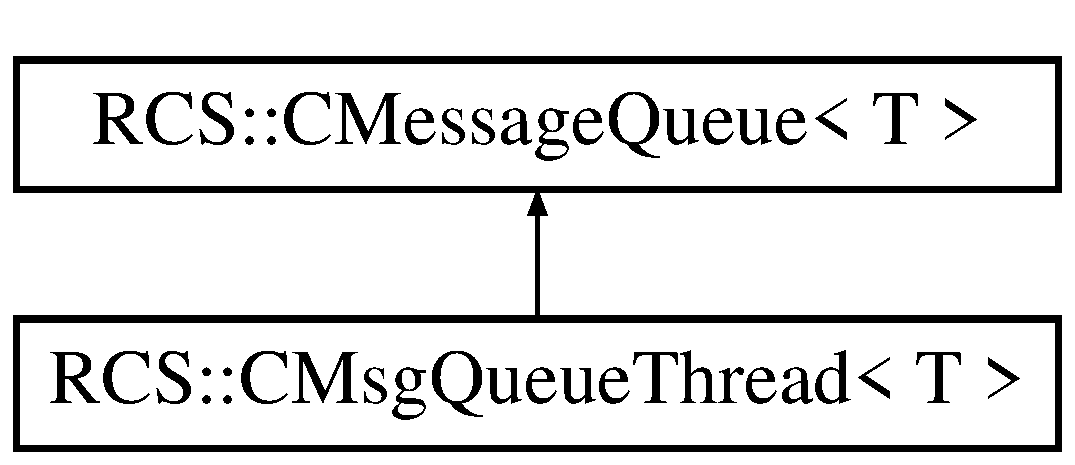
\includegraphics[height=2.000000cm]{classRCS_1_1CMessageQueue}
\end{center}
\end{figure}
\subsection*{Public Types}
\begin{DoxyCompactItemize}
\item 
typedef std\-::deque$<$ T $>$ \hyperlink{classRCS_1_1CMessageQueue_a272ec6240c0ae616f66e71a033326e28}{xml\-\_\-message\-\_\-queue}
\item 
typedef std\-::deque$<$ T $>$\-::iterator \hyperlink{classRCS_1_1CMessageQueue_aa229add119e43aa53229252b6dffb691}{xml\-\_\-message\-\_\-queue\-\_\-iterator}
\end{DoxyCompactItemize}
\subsection*{Public Member Functions}
\begin{DoxyCompactItemize}
\item 
\hyperlink{classRCS_1_1CMessageQueue_afa0f086027abffe37b9e9673396f7b00}{C\-Message\-Queue} ()
\item 
void \hyperlink{classRCS_1_1CMessageQueue_a1fbabdd6e6aaf02572a93531ed871559}{Clear\-Msg\-Queue} ()
\begin{DoxyCompactList}\small\item\em Clear\-Msg\-Queue clears all contents in message queue. T. \end{DoxyCompactList}\item 
size\-\_\-t \hyperlink{classRCS_1_1CMessageQueue_a7929c4ce871eab3dfb8dfabd5bf4bdb9}{Size\-Msg\-Queue} ()
\begin{DoxyCompactList}\small\item\em Size\-Msg\-Queue returns number of items in message queue. \end{DoxyCompactList}\item 
T \hyperlink{classRCS_1_1CMessageQueue_afbde6b0fa4044557ba5f990c69d52ff7}{Pop\-Front\-Msg\-Queue} ()
\begin{DoxyCompactList}\small\item\em Pop\-Front\-Msg\-Queue mutex pop of front item of message queue. \end{DoxyCompactList}\item 
T \hyperlink{classRCS_1_1CMessageQueue_a1c01196dadf55e07e7507a552b94a452}{Peek\-Front\-Msg\-Queue} ()
\begin{DoxyCompactList}\small\item\em Peek\-Front\-Msg\-Queue mutex peeks at front item of message queue. \end{DoxyCompactList}\item 
T \hyperlink{classRCS_1_1CMessageQueue_a5d669a3cecd23be9113567421f2b06a1}{Back\-Msg\-Queue} ()
\begin{DoxyCompactList}\small\item\em Back\-Msg\-Queue mutex retrieves back item of message queue. Does not pop queue. \end{DoxyCompactList}\item 
void \hyperlink{classRCS_1_1CMessageQueue_a1f23fdbd7b3c7c3861abea8fb0899288}{Add\-Msg\-Queue} (T t)
\begin{DoxyCompactList}\small\item\em Add\-Msg\-Queue mutex push to back an item onto message queue. \end{DoxyCompactList}\item 
void \hyperlink{classRCS_1_1CMessageQueue_a975b0dc0f762f129fb6bd9297cbb3a3d}{Add\-Back\-Msg\-Queue} (T t)
\begin{DoxyCompactList}\small\item\em Add\-Msg\-Queue mutex push to back an item onto message queue. \end{DoxyCompactList}\item 
void \hyperlink{classRCS_1_1CMessageQueue_a4da04a657574f94d654898fd0bfc5983}{Add\-Front\-Msg\-Queue} (T t)
\begin{DoxyCompactList}\small\item\em Add\-Msg\-Queue mutex push to front an item onto message queue. \end{DoxyCompactList}\item 
void \hyperlink{classRCS_1_1CMessageQueue_ab9a9aa2c8e05c74bd0b67dc2b576850f}{Insert\-Front\-Msg\-Queue} (T t)
\begin{DoxyCompactList}\small\item\em Insert\-Front\-Msg\-Queue mutex push to front an item onto message queue. \end{DoxyCompactList}\item 
\hyperlink{classRCS_1_1CMessageQueue_aa229add119e43aa53229252b6dffb691}{xml\-\_\-message\-\_\-queue\-\_\-iterator} \hyperlink{classRCS_1_1CMessageQueue_ae8f0f317fd57acac619797badad88be2}{end} ()
\item 
\hyperlink{classRCS_1_1CMessageQueue_aa229add119e43aa53229252b6dffb691}{xml\-\_\-message\-\_\-queue\-\_\-iterator} \hyperlink{classRCS_1_1CMessageQueue_aba32094584981f8b425660cb3ee4cf50}{begin} ()
\end{DoxyCompactItemize}
\subsection*{Protected Attributes}
\begin{DoxyCompactItemize}
\item 
boost\-::mutex \hyperlink{classRCS_1_1CMessageQueue_a874fdf08657e4ca2da89168bb6176c49}{m}
\item 
\hyperlink{classRCS_1_1CMessageQueue_a272ec6240c0ae616f66e71a033326e28}{xml\-\_\-message\-\_\-queue} \hyperlink{classRCS_1_1CMessageQueue_aa699f0b2f9f057242c5f0d3882f14ecb}{xml\-\_\-msgs}
\end{DoxyCompactItemize}


\subsection{Detailed Description}
\subsubsection*{template$<$typename T$>$class R\-C\-S\-::\-C\-Message\-Queue$<$ T $>$}

The \hyperlink{classRCS_1_1CMessageQueue}{C\-Message\-Queue} offers a mutexed front to a S\-T\-L/std deque. The queue is a L\-I\-F\-O data structure. Useful for safely sharing data between multiple threads. 

\subsection{Member Typedef Documentation}
\hypertarget{classRCS_1_1CMessageQueue_a272ec6240c0ae616f66e71a033326e28}{\index{R\-C\-S\-::\-C\-Message\-Queue@{R\-C\-S\-::\-C\-Message\-Queue}!xml\-\_\-message\-\_\-queue@{xml\-\_\-message\-\_\-queue}}
\index{xml\-\_\-message\-\_\-queue@{xml\-\_\-message\-\_\-queue}!RCS::CMessageQueue@{R\-C\-S\-::\-C\-Message\-Queue}}
\subsubsection[{xml\-\_\-message\-\_\-queue}]{\setlength{\rightskip}{0pt plus 5cm}template$<$typename T$>$ typedef std\-::deque$<$T$>$ {\bf R\-C\-S\-::\-C\-Message\-Queue}$<$ T $>$\-::{\bf xml\-\_\-message\-\_\-queue}}}\label{classRCS_1_1CMessageQueue_a272ec6240c0ae616f66e71a033326e28}
\hypertarget{classRCS_1_1CMessageQueue_aa229add119e43aa53229252b6dffb691}{\index{R\-C\-S\-::\-C\-Message\-Queue@{R\-C\-S\-::\-C\-Message\-Queue}!xml\-\_\-message\-\_\-queue\-\_\-iterator@{xml\-\_\-message\-\_\-queue\-\_\-iterator}}
\index{xml\-\_\-message\-\_\-queue\-\_\-iterator@{xml\-\_\-message\-\_\-queue\-\_\-iterator}!RCS::CMessageQueue@{R\-C\-S\-::\-C\-Message\-Queue}}
\subsubsection[{xml\-\_\-message\-\_\-queue\-\_\-iterator}]{\setlength{\rightskip}{0pt plus 5cm}template$<$typename T$>$ typedef std\-::deque$<$T$>$\-::iterator {\bf R\-C\-S\-::\-C\-Message\-Queue}$<$ T $>$\-::{\bf xml\-\_\-message\-\_\-queue\-\_\-iterator}}}\label{classRCS_1_1CMessageQueue_aa229add119e43aa53229252b6dffb691}


\subsection{Constructor \& Destructor Documentation}
\hypertarget{classRCS_1_1CMessageQueue_afa0f086027abffe37b9e9673396f7b00}{\index{R\-C\-S\-::\-C\-Message\-Queue@{R\-C\-S\-::\-C\-Message\-Queue}!C\-Message\-Queue@{C\-Message\-Queue}}
\index{C\-Message\-Queue@{C\-Message\-Queue}!RCS::CMessageQueue@{R\-C\-S\-::\-C\-Message\-Queue}}
\subsubsection[{C\-Message\-Queue}]{\setlength{\rightskip}{0pt plus 5cm}template$<$typename T$>$ {\bf R\-C\-S\-::\-C\-Message\-Queue}$<$ T $>$\-::{\bf C\-Message\-Queue} (
\begin{DoxyParamCaption}
{}
\end{DoxyParamCaption}
)\hspace{0.3cm}{\ttfamily [inline]}}}\label{classRCS_1_1CMessageQueue_afa0f086027abffe37b9e9673396f7b00}


\subsection{Member Function Documentation}
\hypertarget{classRCS_1_1CMessageQueue_a975b0dc0f762f129fb6bd9297cbb3a3d}{\index{R\-C\-S\-::\-C\-Message\-Queue@{R\-C\-S\-::\-C\-Message\-Queue}!Add\-Back\-Msg\-Queue@{Add\-Back\-Msg\-Queue}}
\index{Add\-Back\-Msg\-Queue@{Add\-Back\-Msg\-Queue}!RCS::CMessageQueue@{R\-C\-S\-::\-C\-Message\-Queue}}
\subsubsection[{Add\-Back\-Msg\-Queue}]{\setlength{\rightskip}{0pt plus 5cm}template$<$typename T$>$ void {\bf R\-C\-S\-::\-C\-Message\-Queue}$<$ T $>$\-::Add\-Back\-Msg\-Queue (
\begin{DoxyParamCaption}
\item[{T}]{t}
\end{DoxyParamCaption}
)\hspace{0.3cm}{\ttfamily [inline]}}}\label{classRCS_1_1CMessageQueue_a975b0dc0f762f129fb6bd9297cbb3a3d}


Add\-Msg\-Queue mutex push to back an item onto message queue. 


\begin{DoxyParams}{Parameters}
{\em T} & item to place in back of message queue. \\
\hline
\end{DoxyParams}
\hypertarget{classRCS_1_1CMessageQueue_a4da04a657574f94d654898fd0bfc5983}{\index{R\-C\-S\-::\-C\-Message\-Queue@{R\-C\-S\-::\-C\-Message\-Queue}!Add\-Front\-Msg\-Queue@{Add\-Front\-Msg\-Queue}}
\index{Add\-Front\-Msg\-Queue@{Add\-Front\-Msg\-Queue}!RCS::CMessageQueue@{R\-C\-S\-::\-C\-Message\-Queue}}
\subsubsection[{Add\-Front\-Msg\-Queue}]{\setlength{\rightskip}{0pt plus 5cm}template$<$typename T$>$ void {\bf R\-C\-S\-::\-C\-Message\-Queue}$<$ T $>$\-::Add\-Front\-Msg\-Queue (
\begin{DoxyParamCaption}
\item[{T}]{t}
\end{DoxyParamCaption}
)\hspace{0.3cm}{\ttfamily [inline]}}}\label{classRCS_1_1CMessageQueue_a4da04a657574f94d654898fd0bfc5983}


Add\-Msg\-Queue mutex push to front an item onto message queue. 


\begin{DoxyParams}{Parameters}
{\em T} & item to place in front of message queue. \\
\hline
\end{DoxyParams}
\hypertarget{classRCS_1_1CMessageQueue_a1f23fdbd7b3c7c3861abea8fb0899288}{\index{R\-C\-S\-::\-C\-Message\-Queue@{R\-C\-S\-::\-C\-Message\-Queue}!Add\-Msg\-Queue@{Add\-Msg\-Queue}}
\index{Add\-Msg\-Queue@{Add\-Msg\-Queue}!RCS::CMessageQueue@{R\-C\-S\-::\-C\-Message\-Queue}}
\subsubsection[{Add\-Msg\-Queue}]{\setlength{\rightskip}{0pt plus 5cm}template$<$typename T$>$ void {\bf R\-C\-S\-::\-C\-Message\-Queue}$<$ T $>$\-::Add\-Msg\-Queue (
\begin{DoxyParamCaption}
\item[{T}]{t}
\end{DoxyParamCaption}
)\hspace{0.3cm}{\ttfamily [inline]}}}\label{classRCS_1_1CMessageQueue_a1f23fdbd7b3c7c3861abea8fb0899288}


Add\-Msg\-Queue mutex push to back an item onto message queue. 


\begin{DoxyParams}{Parameters}
{\em T} & item to place in back of message queue. \\
\hline
\end{DoxyParams}
\hypertarget{classRCS_1_1CMessageQueue_a5d669a3cecd23be9113567421f2b06a1}{\index{R\-C\-S\-::\-C\-Message\-Queue@{R\-C\-S\-::\-C\-Message\-Queue}!Back\-Msg\-Queue@{Back\-Msg\-Queue}}
\index{Back\-Msg\-Queue@{Back\-Msg\-Queue}!RCS::CMessageQueue@{R\-C\-S\-::\-C\-Message\-Queue}}
\subsubsection[{Back\-Msg\-Queue}]{\setlength{\rightskip}{0pt plus 5cm}template$<$typename T$>$ T {\bf R\-C\-S\-::\-C\-Message\-Queue}$<$ T $>$\-::Back\-Msg\-Queue (
\begin{DoxyParamCaption}
{}
\end{DoxyParamCaption}
)\hspace{0.3cm}{\ttfamily [inline]}}}\label{classRCS_1_1CMessageQueue_a5d669a3cecd23be9113567421f2b06a1}


Back\-Msg\-Queue mutex retrieves back item of message queue. Does not pop queue. 

\begin{DoxyReturn}{Returns}
T returns back item from message queue. 
\end{DoxyReturn}
\hypertarget{classRCS_1_1CMessageQueue_aba32094584981f8b425660cb3ee4cf50}{\index{R\-C\-S\-::\-C\-Message\-Queue@{R\-C\-S\-::\-C\-Message\-Queue}!begin@{begin}}
\index{begin@{begin}!RCS::CMessageQueue@{R\-C\-S\-::\-C\-Message\-Queue}}
\subsubsection[{begin}]{\setlength{\rightskip}{0pt plus 5cm}template$<$typename T$>$ {\bf xml\-\_\-message\-\_\-queue\-\_\-iterator} {\bf R\-C\-S\-::\-C\-Message\-Queue}$<$ T $>$\-::begin (
\begin{DoxyParamCaption}
{}
\end{DoxyParamCaption}
)\hspace{0.3cm}{\ttfamily [inline]}}}\label{classRCS_1_1CMessageQueue_aba32094584981f8b425660cb3ee4cf50}
\hypertarget{classRCS_1_1CMessageQueue_a1fbabdd6e6aaf02572a93531ed871559}{\index{R\-C\-S\-::\-C\-Message\-Queue@{R\-C\-S\-::\-C\-Message\-Queue}!Clear\-Msg\-Queue@{Clear\-Msg\-Queue}}
\index{Clear\-Msg\-Queue@{Clear\-Msg\-Queue}!RCS::CMessageQueue@{R\-C\-S\-::\-C\-Message\-Queue}}
\subsubsection[{Clear\-Msg\-Queue}]{\setlength{\rightskip}{0pt plus 5cm}template$<$typename T$>$ void {\bf R\-C\-S\-::\-C\-Message\-Queue}$<$ T $>$\-::Clear\-Msg\-Queue (
\begin{DoxyParamCaption}
{}
\end{DoxyParamCaption}
)\hspace{0.3cm}{\ttfamily [inline]}}}\label{classRCS_1_1CMessageQueue_a1fbabdd6e6aaf02572a93531ed871559}


Clear\-Msg\-Queue clears all contents in message queue. T. 

\hypertarget{classRCS_1_1CMessageQueue_ae8f0f317fd57acac619797badad88be2}{\index{R\-C\-S\-::\-C\-Message\-Queue@{R\-C\-S\-::\-C\-Message\-Queue}!end@{end}}
\index{end@{end}!RCS::CMessageQueue@{R\-C\-S\-::\-C\-Message\-Queue}}
\subsubsection[{end}]{\setlength{\rightskip}{0pt plus 5cm}template$<$typename T$>$ {\bf xml\-\_\-message\-\_\-queue\-\_\-iterator} {\bf R\-C\-S\-::\-C\-Message\-Queue}$<$ T $>$\-::end (
\begin{DoxyParamCaption}
{}
\end{DoxyParamCaption}
)\hspace{0.3cm}{\ttfamily [inline]}}}\label{classRCS_1_1CMessageQueue_ae8f0f317fd57acac619797badad88be2}
\hypertarget{classRCS_1_1CMessageQueue_ab9a9aa2c8e05c74bd0b67dc2b576850f}{\index{R\-C\-S\-::\-C\-Message\-Queue@{R\-C\-S\-::\-C\-Message\-Queue}!Insert\-Front\-Msg\-Queue@{Insert\-Front\-Msg\-Queue}}
\index{Insert\-Front\-Msg\-Queue@{Insert\-Front\-Msg\-Queue}!RCS::CMessageQueue@{R\-C\-S\-::\-C\-Message\-Queue}}
\subsubsection[{Insert\-Front\-Msg\-Queue}]{\setlength{\rightskip}{0pt plus 5cm}template$<$typename T$>$ void {\bf R\-C\-S\-::\-C\-Message\-Queue}$<$ T $>$\-::Insert\-Front\-Msg\-Queue (
\begin{DoxyParamCaption}
\item[{T}]{t}
\end{DoxyParamCaption}
)\hspace{0.3cm}{\ttfamily [inline]}}}\label{classRCS_1_1CMessageQueue_ab9a9aa2c8e05c74bd0b67dc2b576850f}


Insert\-Front\-Msg\-Queue mutex push to front an item onto message queue. 


\begin{DoxyParams}{Parameters}
{\em T} & item to place in front of message queue. \\
\hline
\end{DoxyParams}
\hypertarget{classRCS_1_1CMessageQueue_a1c01196dadf55e07e7507a552b94a452}{\index{R\-C\-S\-::\-C\-Message\-Queue@{R\-C\-S\-::\-C\-Message\-Queue}!Peek\-Front\-Msg\-Queue@{Peek\-Front\-Msg\-Queue}}
\index{Peek\-Front\-Msg\-Queue@{Peek\-Front\-Msg\-Queue}!RCS::CMessageQueue@{R\-C\-S\-::\-C\-Message\-Queue}}
\subsubsection[{Peek\-Front\-Msg\-Queue}]{\setlength{\rightskip}{0pt plus 5cm}template$<$typename T$>$ T {\bf R\-C\-S\-::\-C\-Message\-Queue}$<$ T $>$\-::Peek\-Front\-Msg\-Queue (
\begin{DoxyParamCaption}
{}
\end{DoxyParamCaption}
)\hspace{0.3cm}{\ttfamily [inline]}}}\label{classRCS_1_1CMessageQueue_a1c01196dadf55e07e7507a552b94a452}


Peek\-Front\-Msg\-Queue mutex peeks at front item of message queue. 

\begin{DoxyReturn}{Returns}
T returns front item from message queue. 
\end{DoxyReturn}
\hypertarget{classRCS_1_1CMessageQueue_afbde6b0fa4044557ba5f990c69d52ff7}{\index{R\-C\-S\-::\-C\-Message\-Queue@{R\-C\-S\-::\-C\-Message\-Queue}!Pop\-Front\-Msg\-Queue@{Pop\-Front\-Msg\-Queue}}
\index{Pop\-Front\-Msg\-Queue@{Pop\-Front\-Msg\-Queue}!RCS::CMessageQueue@{R\-C\-S\-::\-C\-Message\-Queue}}
\subsubsection[{Pop\-Front\-Msg\-Queue}]{\setlength{\rightskip}{0pt plus 5cm}template$<$typename T$>$ T {\bf R\-C\-S\-::\-C\-Message\-Queue}$<$ T $>$\-::Pop\-Front\-Msg\-Queue (
\begin{DoxyParamCaption}
{}
\end{DoxyParamCaption}
)\hspace{0.3cm}{\ttfamily [inline]}}}\label{classRCS_1_1CMessageQueue_afbde6b0fa4044557ba5f990c69d52ff7}


Pop\-Front\-Msg\-Queue mutex pop of front item of message queue. 

\begin{DoxyReturn}{Returns}
T returns front item from message queue. 
\end{DoxyReturn}
\hypertarget{classRCS_1_1CMessageQueue_a7929c4ce871eab3dfb8dfabd5bf4bdb9}{\index{R\-C\-S\-::\-C\-Message\-Queue@{R\-C\-S\-::\-C\-Message\-Queue}!Size\-Msg\-Queue@{Size\-Msg\-Queue}}
\index{Size\-Msg\-Queue@{Size\-Msg\-Queue}!RCS::CMessageQueue@{R\-C\-S\-::\-C\-Message\-Queue}}
\subsubsection[{Size\-Msg\-Queue}]{\setlength{\rightskip}{0pt plus 5cm}template$<$typename T$>$ size\-\_\-t {\bf R\-C\-S\-::\-C\-Message\-Queue}$<$ T $>$\-::Size\-Msg\-Queue (
\begin{DoxyParamCaption}
{}
\end{DoxyParamCaption}
)\hspace{0.3cm}{\ttfamily [inline]}}}\label{classRCS_1_1CMessageQueue_a7929c4ce871eab3dfb8dfabd5bf4bdb9}


Size\-Msg\-Queue returns number of items in message queue. 



\subsection{Member Data Documentation}
\hypertarget{classRCS_1_1CMessageQueue_a874fdf08657e4ca2da89168bb6176c49}{\index{R\-C\-S\-::\-C\-Message\-Queue@{R\-C\-S\-::\-C\-Message\-Queue}!m@{m}}
\index{m@{m}!RCS::CMessageQueue@{R\-C\-S\-::\-C\-Message\-Queue}}
\subsubsection[{m}]{\setlength{\rightskip}{0pt plus 5cm}template$<$typename T$>$ boost\-::mutex {\bf R\-C\-S\-::\-C\-Message\-Queue}$<$ T $>$\-::m\hspace{0.3cm}{\ttfamily [protected]}}}\label{classRCS_1_1CMessageQueue_a874fdf08657e4ca2da89168bb6176c49}
\hypertarget{classRCS_1_1CMessageQueue_aa699f0b2f9f057242c5f0d3882f14ecb}{\index{R\-C\-S\-::\-C\-Message\-Queue@{R\-C\-S\-::\-C\-Message\-Queue}!xml\-\_\-msgs@{xml\-\_\-msgs}}
\index{xml\-\_\-msgs@{xml\-\_\-msgs}!RCS::CMessageQueue@{R\-C\-S\-::\-C\-Message\-Queue}}
\subsubsection[{xml\-\_\-msgs}]{\setlength{\rightskip}{0pt plus 5cm}template$<$typename T$>$ {\bf xml\-\_\-message\-\_\-queue} {\bf R\-C\-S\-::\-C\-Message\-Queue}$<$ T $>$\-::xml\-\_\-msgs\hspace{0.3cm}{\ttfamily [protected]}}}\label{classRCS_1_1CMessageQueue_aa699f0b2f9f057242c5f0d3882f14ecb}


The documentation for this class was generated from the following file\-:\begin{DoxyCompactItemize}
\item 
/usr/local/michalos/nistfanuc\-\_\-ws/src/nist\-\_\-fanuc/include/nist\-\_\-fanuc/\-N\-I\-S\-T/\hyperlink{RCSMsgQueue_8h}{R\-C\-S\-Msg\-Queue.\-h}\end{DoxyCompactItemize}

\hypertarget{structNearestJointsLookup_1_1cmp__op}{\section{Nearest\-Joints\-Lookup\-:\-:cmp\-\_\-op Struct Reference}
\label{structNearestJointsLookup_1_1cmp__op}\index{Nearest\-Joints\-Lookup\-::cmp\-\_\-op@{Nearest\-Joints\-Lookup\-::cmp\-\_\-op}}
}


{\ttfamily \#include $<$Demo.\-h$>$}

\subsection*{Public Member Functions}
\begin{DoxyCompactItemize}
\item 
bool \hyperlink{structNearestJointsLookup_1_1cmp__op_a13aa1b5b8df5beefbc16bc0a346b8786}{operator()} (const tf\-::\-Pose \&a, const tf\-::\-Pose \&b)
\end{DoxyCompactItemize}


\subsection{Member Function Documentation}
\hypertarget{structNearestJointsLookup_1_1cmp__op_a13aa1b5b8df5beefbc16bc0a346b8786}{\index{Nearest\-Joints\-Lookup\-::cmp\-\_\-op@{Nearest\-Joints\-Lookup\-::cmp\-\_\-op}!operator()@{operator()}}
\index{operator()@{operator()}!NearestJointsLookup::cmp_op@{Nearest\-Joints\-Lookup\-::cmp\-\_\-op}}
\subsubsection[{operator()}]{\setlength{\rightskip}{0pt plus 5cm}bool Nearest\-Joints\-Lookup\-::cmp\-\_\-op\-::operator() (
\begin{DoxyParamCaption}
\item[{const tf\-::\-Pose \&}]{a, }
\item[{const tf\-::\-Pose \&}]{b}
\end{DoxyParamCaption}
)\hspace{0.3cm}{\ttfamily [inline]}}}\label{structNearestJointsLookup_1_1cmp__op_a13aa1b5b8df5beefbc16bc0a346b8786}


The documentation for this struct was generated from the following file\-:\begin{DoxyCompactItemize}
\item 
/usr/local/michalos/nistfanuc\-\_\-ws/src/nist\-\_\-fanuc/include/nist\-\_\-fanuc/\hyperlink{Demo_8h}{Demo.\-h}\end{DoxyCompactItemize}

\hypertarget{classRCS_1_1CMsgQueueThread}{\section{R\-C\-S\-:\-:C\-Msg\-Queue\-Thread$<$ T $>$ Class Template Reference}
\label{classRCS_1_1CMsgQueueThread}\index{R\-C\-S\-::\-C\-Msg\-Queue\-Thread$<$ T $>$@{R\-C\-S\-::\-C\-Msg\-Queue\-Thread$<$ T $>$}}
}


\hyperlink{classRCS_1_1CMsgQueueThread}{C\-Msg\-Queue\-Thread} is a message queued thread. It is activated when a message is received. \par
 Notes\-: \href{http://stackoverflow.com/questions/768351/complete-example-using-boostsignals-for-c-eventing}{\tt http\-://stackoverflow.\-com/questions/768351/complete-\/example-\/using-\/boostsignals-\/for-\/c-\/eventing}.  




{\ttfamily \#include $<$R\-C\-S\-Msg\-Queue\-Thread.\-h$>$}

Inheritance diagram for R\-C\-S\-:\-:C\-Msg\-Queue\-Thread$<$ T $>$\-:\begin{figure}[H]
\begin{center}
\leavevmode
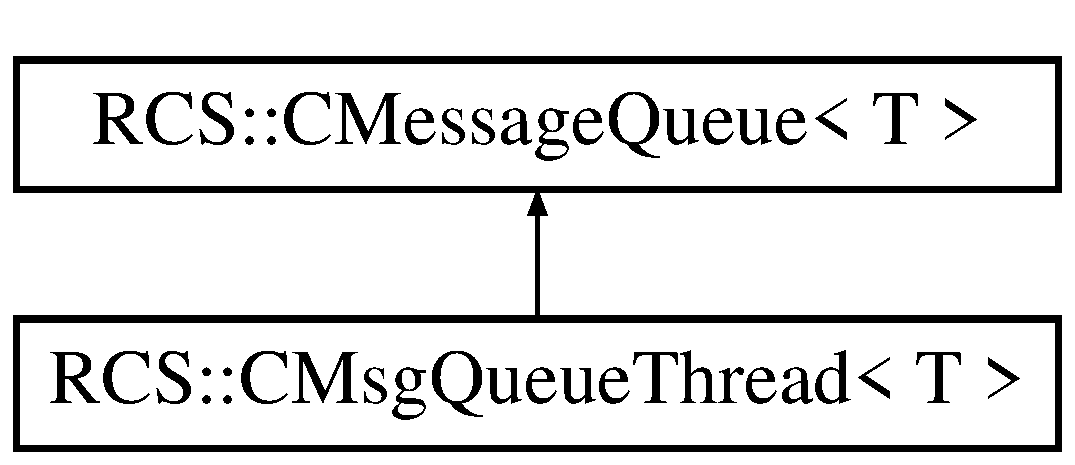
\includegraphics[height=2.000000cm]{classRCS_1_1CMsgQueueThread}
\end{center}
\end{figure}
\subsection*{Public Member Functions}
\begin{DoxyCompactItemize}
\item 
\hyperlink{classRCS_1_1CMsgQueueThread_a0dcb508f3c9faf6ec731bb09578f36e0}{C\-Msg\-Queue\-Thread} ()
\begin{DoxyCompactList}\small\item\em Constructor of thread, that takes cycle time as input. \end{DoxyCompactList}\item 
\hyperlink{classRCS_1_1CMsgQueueThread_ae3ae4576c24fb0c251dd3e5d6db599f3}{$\sim$\-C\-Msg\-Queue\-Thread} ()
\begin{DoxyCompactList}\small\item\em Destructor of thread, makes sure thread has stopped. \end{DoxyCompactList}\item 
virtual void \hyperlink{classRCS_1_1CMsgQueueThread_a84524d066ef68e616d16f53e0f5ff73a}{Add\-Msg\-Queue} (T t)
\item 
std\-::string \& \hyperlink{classRCS_1_1CMsgQueueThread_a2855d2560980c4a734781dc81314cb54}{Name} ()
\begin{DoxyCompactList}\small\item\em Name returns name of thread. \end{DoxyCompactList}\item 
void \hyperlink{classRCS_1_1CMsgQueueThread_ae97cebd1e3f04d7b302de5c9a186fffa}{Join} ()
\begin{DoxyCompactList}\small\item\em Uses boost thread join routine. \end{DoxyCompactList}\item 
virtual void \hyperlink{classRCS_1_1CMsgQueueThread_a43d2b0e9a8811115d2fd805c7291d676}{Init} ()
\begin{DoxyCompactList}\small\item\em Init function called before \hyperlink{classRCS_1_1CMsgQueueThread_ac348fb5db221c3a6502a15f60963e047}{Action()} loop. \end{DoxyCompactList}\item 
virtual void \hyperlink{classRCS_1_1CMsgQueueThread_a602660a933db171f91f52531fbff0fcf}{Cleanup} ()
\begin{DoxyCompactList}\small\item\em Cleanup function called after \hyperlink{classRCS_1_1CMsgQueueThread_ac348fb5db221c3a6502a15f60963e047}{Action()} loop done. \end{DoxyCompactList}\item 
virtual int \hyperlink{classRCS_1_1CMsgQueueThread_ac348fb5db221c3a6502a15f60963e047}{Action} ()
\begin{DoxyCompactList}\small\item\em Action override function called every cycle. \end{DoxyCompactList}\item 
void \hyperlink{classRCS_1_1CMsgQueueThread_a22265a333cc1260e666c059e3cf66a45}{Start} ()
\begin{DoxyCompactList}\small\item\em Start starts the thread which call \hyperlink{classRCS_1_1CMsgQueueThread_a43d2b0e9a8811115d2fd805c7291d676}{Init()}, and then does \hyperlink{classRCS_1_1CMsgQueueThread_ac348fb5db221c3a6502a15f60963e047}{Action()} loop. \end{DoxyCompactList}\item 
void \hyperlink{classRCS_1_1CMsgQueueThread_ab44bf2c1a6b1aa4130ccb75b60337398}{Stop} (bool b\-Wait=false)
\begin{DoxyCompactList}\small\item\em Stop stops the thread, by notifying the wait condition. \end{DoxyCompactList}\item 
void \hyperlink{classRCS_1_1CMsgQueueThread_a8822227bd0522cb2b32f3c69b2dc8ed1}{Suspend} ()
\begin{DoxyCompactList}\small\item\em Suspend stops the thread loop until restarted with \hyperlink{classRCS_1_1CMsgQueueThread_aa7f583a7ec672c66b2bdb057d2adf63c}{Resume()}. \end{DoxyCompactList}\item 
void \hyperlink{classRCS_1_1CMsgQueueThread_aa7f583a7ec672c66b2bdb057d2adf63c}{Resume} ()
\begin{DoxyCompactList}\small\item\em Resume resume execution of the thread loop stopped with \hyperlink{classRCS_1_1CMsgQueueThread_a8822227bd0522cb2b32f3c69b2dc8ed1}{Suspend()}. \end{DoxyCompactList}\item 
int \& \hyperlink{classRCS_1_1CMsgQueueThread_ad86be410679b125162eef984d7116c91}{Debug\-Level} ()
\begin{DoxyCompactList}\small\item\em Debug\-Level returns the debugging level of the thread. \end{DoxyCompactList}\item 
void \hyperlink{classRCS_1_1CMsgQueueThread_a7474536f6fe1bb89118e8a125b8fbb91}{Cycle} ()
\begin{DoxyCompactList}\small\item\em Cycle is the thread main function. It calls init, action, and cleanup. After each cycle waits exactly amount given by cycle time. \end{DoxyCompactList}\end{DoxyCompactItemize}
\subsection*{Static Public Member Functions}
\begin{DoxyCompactItemize}
\item 
static boost\-::thread\-\_\-group \& \hyperlink{classRCS_1_1CMsgQueueThread_ac70bf2b33ea7f6d3fd2e72206c080a75}{Thread\-Group} ()
\begin{DoxyCompactList}\small\item\em Thread\-Group is a static definition of boost thread group. \end{DoxyCompactList}\item 
static std\-::vector\\*
$<$ \hyperlink{classRCS_1_1CMsgQueueThread}{C\-Msg\-Queue\-Thread} $\ast$ $>$ \& \hyperlink{classRCS_1_1CMsgQueueThread_a8d9a466ec9df7101c94af23ccaaf5727}{Threads} ()
\begin{DoxyCompactList}\small\item\em Threads is a static definition of all the threads that have been created. \end{DoxyCompactList}\item 
static void \hyperlink{classRCS_1_1CMsgQueueThread_a965133948e3f8580b318ed69a5639937}{Stop\-All} ()
\begin{DoxyCompactList}\small\item\em Static Stop\-All which stops all the threads created in the boost thread group. \end{DoxyCompactList}\end{DoxyCompactItemize}
\subsection*{Protected Attributes}
\begin{DoxyCompactItemize}
\item 
std\-::string \hyperlink{classRCS_1_1CMsgQueueThread_a73e8b77421902303337324d84db7d35e}{\-\_\-name}
\item 
int \hyperlink{classRCS_1_1CMsgQueueThread_af5f49a26ae621445fb7034f9f22eee9e}{\-\_\-debug\-Level}
\item 
bool \hyperlink{classRCS_1_1CMsgQueueThread_abaca84c63f4938c14feb681aaa3065fa}{\-\_\-b\-Done}
\item 
boost\-::thread \hyperlink{classRCS_1_1CMsgQueueThread_afe3a75cabe791747c8d1464014e1f798}{m\-\_\-thread}
\item 
boost\-::signals2\-::signal$<$ int()$>$ \hyperlink{classRCS_1_1CMsgQueueThread_ad4d34f744d23222ec66655fbcb6a2580}{Sig\-Action}
\item 
boost\-::mutex \hyperlink{classRCS_1_1CMsgQueueThread_a238d69660145a0aaaf44822073c353bf}{m}
\item 
boost\-::mutex \hyperlink{classRCS_1_1CMsgQueueThread_a45804784a5293cc44bec276842b8eb0a}{stop\-Mutex}
\item 
boost\-::condition \hyperlink{classRCS_1_1CMsgQueueThread_a2d89255c589626cc327ea0f87e2d03f8}{stop\-Cond}
\end{DoxyCompactItemize}
\subsection*{Additional Inherited Members}


\subsection{Detailed Description}
\subsubsection*{template$<$typename T$>$class R\-C\-S\-::\-C\-Msg\-Queue\-Thread$<$ T $>$}

\hyperlink{classRCS_1_1CMsgQueueThread}{C\-Msg\-Queue\-Thread} is a message queued thread. It is activated when a message is received. \par
 Notes\-: \href{http://stackoverflow.com/questions/768351/complete-example-using-boostsignals-for-c-eventing}{\tt http\-://stackoverflow.\-com/questions/768351/complete-\/example-\/using-\/boostsignals-\/for-\/c-\/eventing}. 

\subsection{Constructor \& Destructor Documentation}
\hypertarget{classRCS_1_1CMsgQueueThread_a0dcb508f3c9faf6ec731bb09578f36e0}{\index{R\-C\-S\-::\-C\-Msg\-Queue\-Thread@{R\-C\-S\-::\-C\-Msg\-Queue\-Thread}!C\-Msg\-Queue\-Thread@{C\-Msg\-Queue\-Thread}}
\index{C\-Msg\-Queue\-Thread@{C\-Msg\-Queue\-Thread}!RCS::CMsgQueueThread@{R\-C\-S\-::\-C\-Msg\-Queue\-Thread}}
\subsubsection[{C\-Msg\-Queue\-Thread}]{\setlength{\rightskip}{0pt plus 5cm}template$<$typename T $>$ {\bf R\-C\-S\-::\-C\-Msg\-Queue\-Thread}$<$ T $>$\-::{\bf C\-Msg\-Queue\-Thread} (
\begin{DoxyParamCaption}
{}
\end{DoxyParamCaption}
)\hspace{0.3cm}{\ttfamily [inline]}}}\label{classRCS_1_1CMsgQueueThread_a0dcb508f3c9faf6ec731bb09578f36e0}


Constructor of thread, that takes cycle time as input. 

\hypertarget{classRCS_1_1CMsgQueueThread_ae3ae4576c24fb0c251dd3e5d6db599f3}{\index{R\-C\-S\-::\-C\-Msg\-Queue\-Thread@{R\-C\-S\-::\-C\-Msg\-Queue\-Thread}!$\sim$\-C\-Msg\-Queue\-Thread@{$\sim$\-C\-Msg\-Queue\-Thread}}
\index{$\sim$\-C\-Msg\-Queue\-Thread@{$\sim$\-C\-Msg\-Queue\-Thread}!RCS::CMsgQueueThread@{R\-C\-S\-::\-C\-Msg\-Queue\-Thread}}
\subsubsection[{$\sim$\-C\-Msg\-Queue\-Thread}]{\setlength{\rightskip}{0pt plus 5cm}template$<$typename T $>$ {\bf R\-C\-S\-::\-C\-Msg\-Queue\-Thread}$<$ T $>$\-::$\sim${\bf C\-Msg\-Queue\-Thread} (
\begin{DoxyParamCaption}
{}
\end{DoxyParamCaption}
)\hspace{0.3cm}{\ttfamily [inline]}}}\label{classRCS_1_1CMsgQueueThread_ae3ae4576c24fb0c251dd3e5d6db599f3}


Destructor of thread, makes sure thread has stopped. 



\subsection{Member Function Documentation}
\hypertarget{classRCS_1_1CMsgQueueThread_ac348fb5db221c3a6502a15f60963e047}{\index{R\-C\-S\-::\-C\-Msg\-Queue\-Thread@{R\-C\-S\-::\-C\-Msg\-Queue\-Thread}!Action@{Action}}
\index{Action@{Action}!RCS::CMsgQueueThread@{R\-C\-S\-::\-C\-Msg\-Queue\-Thread}}
\subsubsection[{Action}]{\setlength{\rightskip}{0pt plus 5cm}template$<$typename T $>$ virtual int {\bf R\-C\-S\-::\-C\-Msg\-Queue\-Thread}$<$ T $>$\-::Action (
\begin{DoxyParamCaption}
{}
\end{DoxyParamCaption}
)\hspace{0.3cm}{\ttfamily [inline]}, {\ttfamily [virtual]}}}\label{classRCS_1_1CMsgQueueThread_ac348fb5db221c3a6502a15f60963e047}


Action override function called every cycle. 

\hypertarget{classRCS_1_1CMsgQueueThread_a84524d066ef68e616d16f53e0f5ff73a}{\index{R\-C\-S\-::\-C\-Msg\-Queue\-Thread@{R\-C\-S\-::\-C\-Msg\-Queue\-Thread}!Add\-Msg\-Queue@{Add\-Msg\-Queue}}
\index{Add\-Msg\-Queue@{Add\-Msg\-Queue}!RCS::CMsgQueueThread@{R\-C\-S\-::\-C\-Msg\-Queue\-Thread}}
\subsubsection[{Add\-Msg\-Queue}]{\setlength{\rightskip}{0pt plus 5cm}template$<$typename T $>$ virtual void {\bf R\-C\-S\-::\-C\-Msg\-Queue\-Thread}$<$ T $>$\-::Add\-Msg\-Queue (
\begin{DoxyParamCaption}
\item[{T}]{t}
\end{DoxyParamCaption}
)\hspace{0.3cm}{\ttfamily [inline]}, {\ttfamily [virtual]}}}\label{classRCS_1_1CMsgQueueThread_a84524d066ef68e616d16f53e0f5ff73a}
\hypertarget{classRCS_1_1CMsgQueueThread_a602660a933db171f91f52531fbff0fcf}{\index{R\-C\-S\-::\-C\-Msg\-Queue\-Thread@{R\-C\-S\-::\-C\-Msg\-Queue\-Thread}!Cleanup@{Cleanup}}
\index{Cleanup@{Cleanup}!RCS::CMsgQueueThread@{R\-C\-S\-::\-C\-Msg\-Queue\-Thread}}
\subsubsection[{Cleanup}]{\setlength{\rightskip}{0pt plus 5cm}template$<$typename T $>$ virtual void {\bf R\-C\-S\-::\-C\-Msg\-Queue\-Thread}$<$ T $>$\-::Cleanup (
\begin{DoxyParamCaption}
{}
\end{DoxyParamCaption}
)\hspace{0.3cm}{\ttfamily [inline]}, {\ttfamily [virtual]}}}\label{classRCS_1_1CMsgQueueThread_a602660a933db171f91f52531fbff0fcf}


Cleanup function called after \hyperlink{classRCS_1_1CMsgQueueThread_ac348fb5db221c3a6502a15f60963e047}{Action()} loop done. 

\hypertarget{classRCS_1_1CMsgQueueThread_a7474536f6fe1bb89118e8a125b8fbb91}{\index{R\-C\-S\-::\-C\-Msg\-Queue\-Thread@{R\-C\-S\-::\-C\-Msg\-Queue\-Thread}!Cycle@{Cycle}}
\index{Cycle@{Cycle}!RCS::CMsgQueueThread@{R\-C\-S\-::\-C\-Msg\-Queue\-Thread}}
\subsubsection[{Cycle}]{\setlength{\rightskip}{0pt plus 5cm}template$<$typename T $>$ void {\bf R\-C\-S\-::\-C\-Msg\-Queue\-Thread}$<$ T $>$\-::Cycle (
\begin{DoxyParamCaption}
{}
\end{DoxyParamCaption}
)\hspace{0.3cm}{\ttfamily [inline]}}}\label{classRCS_1_1CMsgQueueThread_a7474536f6fe1bb89118e8a125b8fbb91}


Cycle is the thread main function. It calls init, action, and cleanup. After each cycle waits exactly amount given by cycle time. 

\hypertarget{classRCS_1_1CMsgQueueThread_ad86be410679b125162eef984d7116c91}{\index{R\-C\-S\-::\-C\-Msg\-Queue\-Thread@{R\-C\-S\-::\-C\-Msg\-Queue\-Thread}!Debug\-Level@{Debug\-Level}}
\index{Debug\-Level@{Debug\-Level}!RCS::CMsgQueueThread@{R\-C\-S\-::\-C\-Msg\-Queue\-Thread}}
\subsubsection[{Debug\-Level}]{\setlength{\rightskip}{0pt plus 5cm}template$<$typename T $>$ int\& {\bf R\-C\-S\-::\-C\-Msg\-Queue\-Thread}$<$ T $>$\-::Debug\-Level (
\begin{DoxyParamCaption}
{}
\end{DoxyParamCaption}
)\hspace{0.3cm}{\ttfamily [inline]}}}\label{classRCS_1_1CMsgQueueThread_ad86be410679b125162eef984d7116c91}


Debug\-Level returns the debugging level of the thread. 

\begin{DoxyReturn}{Returns}
int returns debug dlvel of thread. 
\end{DoxyReturn}
\hypertarget{classRCS_1_1CMsgQueueThread_a43d2b0e9a8811115d2fd805c7291d676}{\index{R\-C\-S\-::\-C\-Msg\-Queue\-Thread@{R\-C\-S\-::\-C\-Msg\-Queue\-Thread}!Init@{Init}}
\index{Init@{Init}!RCS::CMsgQueueThread@{R\-C\-S\-::\-C\-Msg\-Queue\-Thread}}
\subsubsection[{Init}]{\setlength{\rightskip}{0pt plus 5cm}template$<$typename T $>$ virtual void {\bf R\-C\-S\-::\-C\-Msg\-Queue\-Thread}$<$ T $>$\-::Init (
\begin{DoxyParamCaption}
{}
\end{DoxyParamCaption}
)\hspace{0.3cm}{\ttfamily [inline]}, {\ttfamily [virtual]}}}\label{classRCS_1_1CMsgQueueThread_a43d2b0e9a8811115d2fd805c7291d676}


Init function called before \hyperlink{classRCS_1_1CMsgQueueThread_ac348fb5db221c3a6502a15f60963e047}{Action()} loop. 

\hypertarget{classRCS_1_1CMsgQueueThread_ae97cebd1e3f04d7b302de5c9a186fffa}{\index{R\-C\-S\-::\-C\-Msg\-Queue\-Thread@{R\-C\-S\-::\-C\-Msg\-Queue\-Thread}!Join@{Join}}
\index{Join@{Join}!RCS::CMsgQueueThread@{R\-C\-S\-::\-C\-Msg\-Queue\-Thread}}
\subsubsection[{Join}]{\setlength{\rightskip}{0pt plus 5cm}template$<$typename T $>$ void {\bf R\-C\-S\-::\-C\-Msg\-Queue\-Thread}$<$ T $>$\-::Join (
\begin{DoxyParamCaption}
{}
\end{DoxyParamCaption}
)\hspace{0.3cm}{\ttfamily [inline]}}}\label{classRCS_1_1CMsgQueueThread_ae97cebd1e3f04d7b302de5c9a186fffa}


Uses boost thread join routine. 

\hypertarget{classRCS_1_1CMsgQueueThread_a2855d2560980c4a734781dc81314cb54}{\index{R\-C\-S\-::\-C\-Msg\-Queue\-Thread@{R\-C\-S\-::\-C\-Msg\-Queue\-Thread}!Name@{Name}}
\index{Name@{Name}!RCS::CMsgQueueThread@{R\-C\-S\-::\-C\-Msg\-Queue\-Thread}}
\subsubsection[{Name}]{\setlength{\rightskip}{0pt plus 5cm}template$<$typename T $>$ std\-::string\& {\bf R\-C\-S\-::\-C\-Msg\-Queue\-Thread}$<$ T $>$\-::Name (
\begin{DoxyParamCaption}
{}
\end{DoxyParamCaption}
)\hspace{0.3cm}{\ttfamily [inline]}}}\label{classRCS_1_1CMsgQueueThread_a2855d2560980c4a734781dc81314cb54}


Name returns name of thread. 

\hypertarget{classRCS_1_1CMsgQueueThread_aa7f583a7ec672c66b2bdb057d2adf63c}{\index{R\-C\-S\-::\-C\-Msg\-Queue\-Thread@{R\-C\-S\-::\-C\-Msg\-Queue\-Thread}!Resume@{Resume}}
\index{Resume@{Resume}!RCS::CMsgQueueThread@{R\-C\-S\-::\-C\-Msg\-Queue\-Thread}}
\subsubsection[{Resume}]{\setlength{\rightskip}{0pt plus 5cm}template$<$typename T $>$ void {\bf R\-C\-S\-::\-C\-Msg\-Queue\-Thread}$<$ T $>$\-::Resume (
\begin{DoxyParamCaption}
{}
\end{DoxyParamCaption}
)\hspace{0.3cm}{\ttfamily [inline]}}}\label{classRCS_1_1CMsgQueueThread_aa7f583a7ec672c66b2bdb057d2adf63c}


Resume resume execution of the thread loop stopped with \hyperlink{classRCS_1_1CMsgQueueThread_a8822227bd0522cb2b32f3c69b2dc8ed1}{Suspend()}. 

\hypertarget{classRCS_1_1CMsgQueueThread_a22265a333cc1260e666c059e3cf66a45}{\index{R\-C\-S\-::\-C\-Msg\-Queue\-Thread@{R\-C\-S\-::\-C\-Msg\-Queue\-Thread}!Start@{Start}}
\index{Start@{Start}!RCS::CMsgQueueThread@{R\-C\-S\-::\-C\-Msg\-Queue\-Thread}}
\subsubsection[{Start}]{\setlength{\rightskip}{0pt plus 5cm}template$<$typename T $>$ void {\bf R\-C\-S\-::\-C\-Msg\-Queue\-Thread}$<$ T $>$\-::Start (
\begin{DoxyParamCaption}
{}
\end{DoxyParamCaption}
)\hspace{0.3cm}{\ttfamily [inline]}}}\label{classRCS_1_1CMsgQueueThread_a22265a333cc1260e666c059e3cf66a45}


Start starts the thread which call \hyperlink{classRCS_1_1CMsgQueueThread_a43d2b0e9a8811115d2fd805c7291d676}{Init()}, and then does \hyperlink{classRCS_1_1CMsgQueueThread_ac348fb5db221c3a6502a15f60963e047}{Action()} loop. 

\hypertarget{classRCS_1_1CMsgQueueThread_ab44bf2c1a6b1aa4130ccb75b60337398}{\index{R\-C\-S\-::\-C\-Msg\-Queue\-Thread@{R\-C\-S\-::\-C\-Msg\-Queue\-Thread}!Stop@{Stop}}
\index{Stop@{Stop}!RCS::CMsgQueueThread@{R\-C\-S\-::\-C\-Msg\-Queue\-Thread}}
\subsubsection[{Stop}]{\setlength{\rightskip}{0pt plus 5cm}template$<$typename T $>$ void {\bf R\-C\-S\-::\-C\-Msg\-Queue\-Thread}$<$ T $>$\-::Stop (
\begin{DoxyParamCaption}
\item[{bool}]{b\-Wait = {\ttfamily false}}
\end{DoxyParamCaption}
)\hspace{0.3cm}{\ttfamily [inline]}}}\label{classRCS_1_1CMsgQueueThread_ab44bf2c1a6b1aa4130ccb75b60337398}


Stop stops the thread, by notifying the wait condition. 


\begin{DoxyParams}{Parameters}
{\em b\-Wait} & indicates whether to wait until thread has finished. \\
\hline
\end{DoxyParams}
\hypertarget{classRCS_1_1CMsgQueueThread_a965133948e3f8580b318ed69a5639937}{\index{R\-C\-S\-::\-C\-Msg\-Queue\-Thread@{R\-C\-S\-::\-C\-Msg\-Queue\-Thread}!Stop\-All@{Stop\-All}}
\index{Stop\-All@{Stop\-All}!RCS::CMsgQueueThread@{R\-C\-S\-::\-C\-Msg\-Queue\-Thread}}
\subsubsection[{Stop\-All}]{\setlength{\rightskip}{0pt plus 5cm}template$<$typename T $>$ static void {\bf R\-C\-S\-::\-C\-Msg\-Queue\-Thread}$<$ T $>$\-::Stop\-All (
\begin{DoxyParamCaption}
{}
\end{DoxyParamCaption}
)\hspace{0.3cm}{\ttfamily [inline]}, {\ttfamily [static]}}}\label{classRCS_1_1CMsgQueueThread_a965133948e3f8580b318ed69a5639937}


Static Stop\-All which stops all the threads created in the boost thread group. 

\hypertarget{classRCS_1_1CMsgQueueThread_a8822227bd0522cb2b32f3c69b2dc8ed1}{\index{R\-C\-S\-::\-C\-Msg\-Queue\-Thread@{R\-C\-S\-::\-C\-Msg\-Queue\-Thread}!Suspend@{Suspend}}
\index{Suspend@{Suspend}!RCS::CMsgQueueThread@{R\-C\-S\-::\-C\-Msg\-Queue\-Thread}}
\subsubsection[{Suspend}]{\setlength{\rightskip}{0pt plus 5cm}template$<$typename T $>$ void {\bf R\-C\-S\-::\-C\-Msg\-Queue\-Thread}$<$ T $>$\-::Suspend (
\begin{DoxyParamCaption}
{}
\end{DoxyParamCaption}
)\hspace{0.3cm}{\ttfamily [inline]}}}\label{classRCS_1_1CMsgQueueThread_a8822227bd0522cb2b32f3c69b2dc8ed1}


Suspend stops the thread loop until restarted with \hyperlink{classRCS_1_1CMsgQueueThread_aa7f583a7ec672c66b2bdb057d2adf63c}{Resume()}. 

\hypertarget{classRCS_1_1CMsgQueueThread_ac70bf2b33ea7f6d3fd2e72206c080a75}{\index{R\-C\-S\-::\-C\-Msg\-Queue\-Thread@{R\-C\-S\-::\-C\-Msg\-Queue\-Thread}!Thread\-Group@{Thread\-Group}}
\index{Thread\-Group@{Thread\-Group}!RCS::CMsgQueueThread@{R\-C\-S\-::\-C\-Msg\-Queue\-Thread}}
\subsubsection[{Thread\-Group}]{\setlength{\rightskip}{0pt plus 5cm}template$<$typename T $>$ static boost\-::thread\-\_\-group\& {\bf R\-C\-S\-::\-C\-Msg\-Queue\-Thread}$<$ T $>$\-::Thread\-Group (
\begin{DoxyParamCaption}
{}
\end{DoxyParamCaption}
)\hspace{0.3cm}{\ttfamily [inline]}, {\ttfamily [static]}}}\label{classRCS_1_1CMsgQueueThread_ac70bf2b33ea7f6d3fd2e72206c080a75}


Thread\-Group is a static definition of boost thread group. 

\hypertarget{classRCS_1_1CMsgQueueThread_a8d9a466ec9df7101c94af23ccaaf5727}{\index{R\-C\-S\-::\-C\-Msg\-Queue\-Thread@{R\-C\-S\-::\-C\-Msg\-Queue\-Thread}!Threads@{Threads}}
\index{Threads@{Threads}!RCS::CMsgQueueThread@{R\-C\-S\-::\-C\-Msg\-Queue\-Thread}}
\subsubsection[{Threads}]{\setlength{\rightskip}{0pt plus 5cm}template$<$typename T $>$ static std\-::vector$<${\bf C\-Msg\-Queue\-Thread} $\ast$$>$\& {\bf R\-C\-S\-::\-C\-Msg\-Queue\-Thread}$<$ T $>$\-::Threads (
\begin{DoxyParamCaption}
{}
\end{DoxyParamCaption}
)\hspace{0.3cm}{\ttfamily [inline]}, {\ttfamily [static]}}}\label{classRCS_1_1CMsgQueueThread_a8d9a466ec9df7101c94af23ccaaf5727}


Threads is a static definition of all the threads that have been created. 



\subsection{Member Data Documentation}
\hypertarget{classRCS_1_1CMsgQueueThread_abaca84c63f4938c14feb681aaa3065fa}{\index{R\-C\-S\-::\-C\-Msg\-Queue\-Thread@{R\-C\-S\-::\-C\-Msg\-Queue\-Thread}!\-\_\-b\-Done@{\-\_\-b\-Done}}
\index{\-\_\-b\-Done@{\-\_\-b\-Done}!RCS::CMsgQueueThread@{R\-C\-S\-::\-C\-Msg\-Queue\-Thread}}
\subsubsection[{\-\_\-b\-Done}]{\setlength{\rightskip}{0pt plus 5cm}template$<$typename T $>$ bool {\bf R\-C\-S\-::\-C\-Msg\-Queue\-Thread}$<$ T $>$\-::\-\_\-b\-Done\hspace{0.3cm}{\ttfamily [protected]}}}\label{classRCS_1_1CMsgQueueThread_abaca84c63f4938c14feb681aaa3065fa}
boolean indicating whether thread has finished \hypertarget{classRCS_1_1CMsgQueueThread_af5f49a26ae621445fb7034f9f22eee9e}{\index{R\-C\-S\-::\-C\-Msg\-Queue\-Thread@{R\-C\-S\-::\-C\-Msg\-Queue\-Thread}!\-\_\-debug\-Level@{\-\_\-debug\-Level}}
\index{\-\_\-debug\-Level@{\-\_\-debug\-Level}!RCS::CMsgQueueThread@{R\-C\-S\-::\-C\-Msg\-Queue\-Thread}}
\subsubsection[{\-\_\-debug\-Level}]{\setlength{\rightskip}{0pt plus 5cm}template$<$typename T $>$ int {\bf R\-C\-S\-::\-C\-Msg\-Queue\-Thread}$<$ T $>$\-::\-\_\-debug\-Level\hspace{0.3cm}{\ttfamily [protected]}}}\label{classRCS_1_1CMsgQueueThread_af5f49a26ae621445fb7034f9f22eee9e}
debug level of thread \hypertarget{classRCS_1_1CMsgQueueThread_a73e8b77421902303337324d84db7d35e}{\index{R\-C\-S\-::\-C\-Msg\-Queue\-Thread@{R\-C\-S\-::\-C\-Msg\-Queue\-Thread}!\-\_\-name@{\-\_\-name}}
\index{\-\_\-name@{\-\_\-name}!RCS::CMsgQueueThread@{R\-C\-S\-::\-C\-Msg\-Queue\-Thread}}
\subsubsection[{\-\_\-name}]{\setlength{\rightskip}{0pt plus 5cm}template$<$typename T $>$ std\-::string {\bf R\-C\-S\-::\-C\-Msg\-Queue\-Thread}$<$ T $>$\-::\-\_\-name\hspace{0.3cm}{\ttfamily [protected]}}}\label{classRCS_1_1CMsgQueueThread_a73e8b77421902303337324d84db7d35e}
name of thread \hypertarget{classRCS_1_1CMsgQueueThread_a238d69660145a0aaaf44822073c353bf}{\index{R\-C\-S\-::\-C\-Msg\-Queue\-Thread@{R\-C\-S\-::\-C\-Msg\-Queue\-Thread}!m@{m}}
\index{m@{m}!RCS::CMsgQueueThread@{R\-C\-S\-::\-C\-Msg\-Queue\-Thread}}
\subsubsection[{m}]{\setlength{\rightskip}{0pt plus 5cm}template$<$typename T $>$ boost\-::mutex {\bf R\-C\-S\-::\-C\-Msg\-Queue\-Thread}$<$ T $>$\-::m\hspace{0.3cm}{\ttfamily [protected]}}}\label{classRCS_1_1CMsgQueueThread_a238d69660145a0aaaf44822073c353bf}
mutex for signal new message \hypertarget{classRCS_1_1CMsgQueueThread_afe3a75cabe791747c8d1464014e1f798}{\index{R\-C\-S\-::\-C\-Msg\-Queue\-Thread@{R\-C\-S\-::\-C\-Msg\-Queue\-Thread}!m\-\_\-thread@{m\-\_\-thread}}
\index{m\-\_\-thread@{m\-\_\-thread}!RCS::CMsgQueueThread@{R\-C\-S\-::\-C\-Msg\-Queue\-Thread}}
\subsubsection[{m\-\_\-thread}]{\setlength{\rightskip}{0pt plus 5cm}template$<$typename T $>$ boost\-::thread {\bf R\-C\-S\-::\-C\-Msg\-Queue\-Thread}$<$ T $>$\-::m\-\_\-thread\hspace{0.3cm}{\ttfamily [protected]}}}\label{classRCS_1_1CMsgQueueThread_afe3a75cabe791747c8d1464014e1f798}
boost thread \hypertarget{classRCS_1_1CMsgQueueThread_ad4d34f744d23222ec66655fbcb6a2580}{\index{R\-C\-S\-::\-C\-Msg\-Queue\-Thread@{R\-C\-S\-::\-C\-Msg\-Queue\-Thread}!Sig\-Action@{Sig\-Action}}
\index{Sig\-Action@{Sig\-Action}!RCS::CMsgQueueThread@{R\-C\-S\-::\-C\-Msg\-Queue\-Thread}}
\subsubsection[{Sig\-Action}]{\setlength{\rightskip}{0pt plus 5cm}template$<$typename T $>$ boost\-::signals2\-::signal$<$int ()$>$ {\bf R\-C\-S\-::\-C\-Msg\-Queue\-Thread}$<$ T $>$\-::Sig\-Action\hspace{0.3cm}{\ttfamily [protected]}}}\label{classRCS_1_1CMsgQueueThread_ad4d34f744d23222ec66655fbcb6a2580}
signals action method \hypertarget{classRCS_1_1CMsgQueueThread_a2d89255c589626cc327ea0f87e2d03f8}{\index{R\-C\-S\-::\-C\-Msg\-Queue\-Thread@{R\-C\-S\-::\-C\-Msg\-Queue\-Thread}!stop\-Cond@{stop\-Cond}}
\index{stop\-Cond@{stop\-Cond}!RCS::CMsgQueueThread@{R\-C\-S\-::\-C\-Msg\-Queue\-Thread}}
\subsubsection[{stop\-Cond}]{\setlength{\rightskip}{0pt plus 5cm}template$<$typename T $>$ boost\-::condition {\bf R\-C\-S\-::\-C\-Msg\-Queue\-Thread}$<$ T $>$\-::stop\-Cond\hspace{0.3cm}{\ttfamily [protected]}}}\label{classRCS_1_1CMsgQueueThread_a2d89255c589626cc327ea0f87e2d03f8}
condition for stopping \hypertarget{classRCS_1_1CMsgQueueThread_a45804784a5293cc44bec276842b8eb0a}{\index{R\-C\-S\-::\-C\-Msg\-Queue\-Thread@{R\-C\-S\-::\-C\-Msg\-Queue\-Thread}!stop\-Mutex@{stop\-Mutex}}
\index{stop\-Mutex@{stop\-Mutex}!RCS::CMsgQueueThread@{R\-C\-S\-::\-C\-Msg\-Queue\-Thread}}
\subsubsection[{stop\-Mutex}]{\setlength{\rightskip}{0pt plus 5cm}template$<$typename T $>$ boost\-::mutex {\bf R\-C\-S\-::\-C\-Msg\-Queue\-Thread}$<$ T $>$\-::stop\-Mutex\hspace{0.3cm}{\ttfamily [protected]}}}\label{classRCS_1_1CMsgQueueThread_a45804784a5293cc44bec276842b8eb0a}
mutex for stopping 

The documentation for this class was generated from the following file\-:\begin{DoxyCompactItemize}
\item 
/usr/local/michalos/nistfanuc\-\_\-ws/src/nist\-\_\-fanuc/include/nist\-\_\-fanuc/\-N\-I\-S\-T/\hyperlink{RCSMsgQueueThread_8h}{R\-C\-S\-Msg\-Queue\-Thread.\-h}\end{DoxyCompactItemize}

\hypertarget{classCRvizMarker}{\section{C\-Rviz\-Marker Class Reference}
\label{classCRvizMarker}\index{C\-Rviz\-Marker@{C\-Rviz\-Marker}}
}


The \hyperlink{classCRvizMarker}{C\-Rviz\-Marker} provides a C++ class to send markers to rviz. Note you must manually add the rviz subscribe to marker messages. Read here for explanation \href{http://answers.ros.org/question/11135/plotting-a-markerarray-of-spheres-with-rviz/}{\tt http\-://answers.\-ros.\-org/question/11135/plotting-\/a-\/markerarray-\/of-\/spheres-\/with-\/rviz/}.  




{\ttfamily \#include $<$Rviz\-Marker.\-h$>$}

\subsection*{Public Member Functions}
\begin{DoxyCompactItemize}
\item 
\hyperlink{classCRvizMarker_ab1733ac291c06bcf40d58f63415a358a}{C\-Rviz\-Marker} (ros\-::\-Node\-Handle \&nh)
\begin{DoxyCompactList}\small\item\em Constructor for \char`\"{}\-Marker\char`\"{} which sets default marker values... \end{DoxyCompactList}\item 
void \hyperlink{classCRvizMarker_a06a5319e1eecb94204c59a7d05e3da27}{Init} ()
\begin{DoxyCompactList}\small\item\em Initialization routine which subsribes to the \char`\"{}\-Marker\char`\"{} topic.. \end{DoxyCompactList}\item 
int \hyperlink{classCRvizMarker_a877d45842547db1ab1fea545e778d2b1}{Send} (\hyperlink{namespaceRCS_aa07e45d8a50e30064283d2b38087f999}{R\-C\-S\-::\-Pose} p)
\begin{DoxyCompactList}\small\item\em Publish a visualization marker message to the Marker topic. \end{DoxyCompactList}\item 
uint32\-\_\-t \hyperlink{classCRvizMarker_ac94e0f85f53d5d434e26546294d51869}{Set\-Shape} (uint32\-\_\-t \hyperlink{classCRvizMarker_ac71ec52d586b80a1f1fd7889871557c7}{shape})
\begin{DoxyCompactList}\small\item\em Set the marker to be displayed. \end{DoxyCompactList}\item 
void \hyperlink{classCRvizMarker_a8bf342bf1758f484ac9a6caf0fb3c86a}{Set\-Color} (double \hyperlink{classCRvizMarker_af9fab360283313338e57876dfd4f7053}{r}, double \hyperlink{classCRvizMarker_ad57f170c6e6757617c990c255c28ad3c}{g}, double \hyperlink{classCRvizMarker_aef6cbf7b2feda8b072863547c9c0719d}{b}, double \hyperlink{classCRvizMarker_a93c527fccbe4672668b497d5b4976704}{a})
\begin{DoxyCompactList}\small\item\em Set the color of the maker to be displayed. \end{DoxyCompactList}\end{DoxyCompactItemize}
\subsection*{Public Attributes}
\begin{DoxyCompactItemize}
\item 
ros\-::\-Publisher \hyperlink{classCRvizMarker_a5cc00e270e464a0c3be4a73ebd9f5aaa}{marker\-\_\-pub}
\item 
ros\-::\-Node\-Handle \& \hyperlink{classCRvizMarker_ab77f5a091387abda51f1d523ac4657f9}{n}
\item 
uint32\-\_\-t \hyperlink{classCRvizMarker_ac71ec52d586b80a1f1fd7889871557c7}{shape}
\item 
int \hyperlink{classCRvizMarker_adc420093c48e69c28b80ccc0181faab5}{\-\_\-id}
\item 
double \hyperlink{classCRvizMarker_ac023151b88d7a4c06cee4c33a5f8d06d}{scalex}
\item 
double \hyperlink{classCRvizMarker_a9a20dee09e81974042c0fb7bb3ff1384}{scaley}
\item 
double \hyperlink{classCRvizMarker_ad1c888f2a832cbc9447cd830bb04ae56}{scalez}
\item 
double \hyperlink{classCRvizMarker_af9fab360283313338e57876dfd4f7053}{r}
\item 
double \hyperlink{classCRvizMarker_ad57f170c6e6757617c990c255c28ad3c}{g}
\item 
double \hyperlink{classCRvizMarker_aef6cbf7b2feda8b072863547c9c0719d}{b}
\item 
double \hyperlink{classCRvizMarker_a93c527fccbe4672668b497d5b4976704}{a}
\end{DoxyCompactItemize}


\subsection{Detailed Description}
The \hyperlink{classCRvizMarker}{C\-Rviz\-Marker} provides a C++ class to send markers to rviz. Note you must manually add the rviz subscribe to marker messages. Read here for explanation \href{http://answers.ros.org/question/11135/plotting-a-markerarray-of-spheres-with-rviz/}{\tt http\-://answers.\-ros.\-org/question/11135/plotting-\/a-\/markerarray-\/of-\/spheres-\/with-\/rviz/}. 

In the R\-O\-S Electric version of rviz (the latest version), Marker is a proper display type. To show the data from the program you posted, in rviz do\-: Click the \char`\"{}\-Add\char`\"{} button in the \char`\"{}\-Displays\char`\"{} area. Choose \char`\"{}\-Marker\char`\"{} in the type list. Click \char`\"{}\-O\-K\char`\"{}

If it doesn't show immediately (it hung for me the first time), do\-:

Click on the \char`\"{}\-Marker Array Topic\char`\"{} line in the new display entry. This should make an elipsis (\char`\"{}...\char`\"{}) button appear. Click the \char`\"{}...\char`\"{} button. A dialog with currently-\/published Marker\-Array topics should appear. Click on \char`\"{}visualization\-\_\-marker\-\_\-array\char`\"{} (or whatever you have named it). Click \char`\"{}\-O\-K\char`\"{} 

\subsection{Constructor \& Destructor Documentation}
\hypertarget{classCRvizMarker_ab1733ac291c06bcf40d58f63415a358a}{\index{C\-Rviz\-Marker@{C\-Rviz\-Marker}!C\-Rviz\-Marker@{C\-Rviz\-Marker}}
\index{C\-Rviz\-Marker@{C\-Rviz\-Marker}!CRvizMarker@{C\-Rviz\-Marker}}
\subsubsection[{C\-Rviz\-Marker}]{\setlength{\rightskip}{0pt plus 5cm}C\-Rviz\-Marker\-::\-C\-Rviz\-Marker (
\begin{DoxyParamCaption}
\item[{ros\-::\-Node\-Handle \&}]{nh}
\end{DoxyParamCaption}
)}}\label{classCRvizMarker_ab1733ac291c06bcf40d58f63415a358a}


Constructor for \char`\"{}\-Marker\char`\"{} which sets default marker values... 



\subsection{Member Function Documentation}
\hypertarget{classCRvizMarker_a06a5319e1eecb94204c59a7d05e3da27}{\index{C\-Rviz\-Marker@{C\-Rviz\-Marker}!Init@{Init}}
\index{Init@{Init}!CRvizMarker@{C\-Rviz\-Marker}}
\subsubsection[{Init}]{\setlength{\rightskip}{0pt plus 5cm}void C\-Rviz\-Marker\-::\-Init (
\begin{DoxyParamCaption}
{}
\end{DoxyParamCaption}
)}}\label{classCRvizMarker_a06a5319e1eecb94204c59a7d05e3da27}


Initialization routine which subsribes to the \char`\"{}\-Marker\char`\"{} topic.. 

\hypertarget{classCRvizMarker_a877d45842547db1ab1fea545e778d2b1}{\index{C\-Rviz\-Marker@{C\-Rviz\-Marker}!Send@{Send}}
\index{Send@{Send}!CRvizMarker@{C\-Rviz\-Marker}}
\subsubsection[{Send}]{\setlength{\rightskip}{0pt plus 5cm}int C\-Rviz\-Marker\-::\-Send (
\begin{DoxyParamCaption}
\item[{{\bf R\-C\-S\-::\-Pose}}]{p}
\end{DoxyParamCaption}
)}}\label{classCRvizMarker_a877d45842547db1ab1fea545e778d2b1}


Publish a visualization marker message to the Marker topic. 


\begin{DoxyParams}{Parameters}
{\em pose} & p is where the marker is to be placed relative to the base link. \\
\hline
\end{DoxyParams}
\hypertarget{classCRvizMarker_a8bf342bf1758f484ac9a6caf0fb3c86a}{\index{C\-Rviz\-Marker@{C\-Rviz\-Marker}!Set\-Color@{Set\-Color}}
\index{Set\-Color@{Set\-Color}!CRvizMarker@{C\-Rviz\-Marker}}
\subsubsection[{Set\-Color}]{\setlength{\rightskip}{0pt plus 5cm}void C\-Rviz\-Marker\-::\-Set\-Color (
\begin{DoxyParamCaption}
\item[{double}]{r, }
\item[{double}]{g, }
\item[{double}]{b, }
\item[{double}]{a}
\end{DoxyParamCaption}
)}}\label{classCRvizMarker_a8bf342bf1758f484ac9a6caf0fb3c86a}


Set the color of the maker to be displayed. 


\begin{DoxyParams}{Parameters}
{\em red,green.} & blue and alpha are the values used herein. \\
\hline
\end{DoxyParams}
\hypertarget{classCRvizMarker_ac94e0f85f53d5d434e26546294d51869}{\index{C\-Rviz\-Marker@{C\-Rviz\-Marker}!Set\-Shape@{Set\-Shape}}
\index{Set\-Shape@{Set\-Shape}!CRvizMarker@{C\-Rviz\-Marker}}
\subsubsection[{Set\-Shape}]{\setlength{\rightskip}{0pt plus 5cm}uint32\-\_\-t C\-Rviz\-Marker\-::\-Set\-Shape (
\begin{DoxyParamCaption}
\item[{uint32\-\_\-t}]{shape}
\end{DoxyParamCaption}
)}}\label{classCRvizMarker_ac94e0f85f53d5d434e26546294d51869}


Set the marker to be displayed. 


\begin{DoxyParams}{Parameters}
{\em shape} & is the enumeration of the marker type. \\
\hline
\end{DoxyParams}


\subsection{Member Data Documentation}
\hypertarget{classCRvizMarker_adc420093c48e69c28b80ccc0181faab5}{\index{C\-Rviz\-Marker@{C\-Rviz\-Marker}!\-\_\-id@{\-\_\-id}}
\index{\-\_\-id@{\-\_\-id}!CRvizMarker@{C\-Rviz\-Marker}}
\subsubsection[{\-\_\-id}]{\setlength{\rightskip}{0pt plus 5cm}int C\-Rviz\-Marker\-::\-\_\-id}}\label{classCRvizMarker_adc420093c48e69c28b80ccc0181faab5}
\hypertarget{classCRvizMarker_a93c527fccbe4672668b497d5b4976704}{\index{C\-Rviz\-Marker@{C\-Rviz\-Marker}!a@{a}}
\index{a@{a}!CRvizMarker@{C\-Rviz\-Marker}}
\subsubsection[{a}]{\setlength{\rightskip}{0pt plus 5cm}double C\-Rviz\-Marker\-::a}}\label{classCRvizMarker_a93c527fccbe4672668b497d5b4976704}
\hypertarget{classCRvizMarker_aef6cbf7b2feda8b072863547c9c0719d}{\index{C\-Rviz\-Marker@{C\-Rviz\-Marker}!b@{b}}
\index{b@{b}!CRvizMarker@{C\-Rviz\-Marker}}
\subsubsection[{b}]{\setlength{\rightskip}{0pt plus 5cm}double C\-Rviz\-Marker\-::b}}\label{classCRvizMarker_aef6cbf7b2feda8b072863547c9c0719d}
\hypertarget{classCRvizMarker_ad57f170c6e6757617c990c255c28ad3c}{\index{C\-Rviz\-Marker@{C\-Rviz\-Marker}!g@{g}}
\index{g@{g}!CRvizMarker@{C\-Rviz\-Marker}}
\subsubsection[{g}]{\setlength{\rightskip}{0pt plus 5cm}double C\-Rviz\-Marker\-::g}}\label{classCRvizMarker_ad57f170c6e6757617c990c255c28ad3c}
\hypertarget{classCRvizMarker_a5cc00e270e464a0c3be4a73ebd9f5aaa}{\index{C\-Rviz\-Marker@{C\-Rviz\-Marker}!marker\-\_\-pub@{marker\-\_\-pub}}
\index{marker\-\_\-pub@{marker\-\_\-pub}!CRvizMarker@{C\-Rviz\-Marker}}
\subsubsection[{marker\-\_\-pub}]{\setlength{\rightskip}{0pt plus 5cm}ros\-::\-Publisher C\-Rviz\-Marker\-::marker\-\_\-pub}}\label{classCRvizMarker_a5cc00e270e464a0c3be4a73ebd9f5aaa}
\hypertarget{classCRvizMarker_ab77f5a091387abda51f1d523ac4657f9}{\index{C\-Rviz\-Marker@{C\-Rviz\-Marker}!n@{n}}
\index{n@{n}!CRvizMarker@{C\-Rviz\-Marker}}
\subsubsection[{n}]{\setlength{\rightskip}{0pt plus 5cm}ros\-::\-Node\-Handle\& C\-Rviz\-Marker\-::n}}\label{classCRvizMarker_ab77f5a091387abda51f1d523ac4657f9}
\hypertarget{classCRvizMarker_af9fab360283313338e57876dfd4f7053}{\index{C\-Rviz\-Marker@{C\-Rviz\-Marker}!r@{r}}
\index{r@{r}!CRvizMarker@{C\-Rviz\-Marker}}
\subsubsection[{r}]{\setlength{\rightskip}{0pt plus 5cm}double C\-Rviz\-Marker\-::r}}\label{classCRvizMarker_af9fab360283313338e57876dfd4f7053}
\hypertarget{classCRvizMarker_ac023151b88d7a4c06cee4c33a5f8d06d}{\index{C\-Rviz\-Marker@{C\-Rviz\-Marker}!scalex@{scalex}}
\index{scalex@{scalex}!CRvizMarker@{C\-Rviz\-Marker}}
\subsubsection[{scalex}]{\setlength{\rightskip}{0pt plus 5cm}double C\-Rviz\-Marker\-::scalex}}\label{classCRvizMarker_ac023151b88d7a4c06cee4c33a5f8d06d}
\hypertarget{classCRvizMarker_a9a20dee09e81974042c0fb7bb3ff1384}{\index{C\-Rviz\-Marker@{C\-Rviz\-Marker}!scaley@{scaley}}
\index{scaley@{scaley}!CRvizMarker@{C\-Rviz\-Marker}}
\subsubsection[{scaley}]{\setlength{\rightskip}{0pt plus 5cm}double C\-Rviz\-Marker\-::scaley}}\label{classCRvizMarker_a9a20dee09e81974042c0fb7bb3ff1384}
\hypertarget{classCRvizMarker_ad1c888f2a832cbc9447cd830bb04ae56}{\index{C\-Rviz\-Marker@{C\-Rviz\-Marker}!scalez@{scalez}}
\index{scalez@{scalez}!CRvizMarker@{C\-Rviz\-Marker}}
\subsubsection[{scalez}]{\setlength{\rightskip}{0pt plus 5cm}double C\-Rviz\-Marker\-::scalez}}\label{classCRvizMarker_ad1c888f2a832cbc9447cd830bb04ae56}
\hypertarget{classCRvizMarker_ac71ec52d586b80a1f1fd7889871557c7}{\index{C\-Rviz\-Marker@{C\-Rviz\-Marker}!shape@{shape}}
\index{shape@{shape}!CRvizMarker@{C\-Rviz\-Marker}}
\subsubsection[{shape}]{\setlength{\rightskip}{0pt plus 5cm}uint32\-\_\-t C\-Rviz\-Marker\-::shape}}\label{classCRvizMarker_ac71ec52d586b80a1f1fd7889871557c7}


The documentation for this class was generated from the following files\-:\begin{DoxyCompactItemize}
\item 
/usr/local/michalos/github/usnistgov/el-\/robotics-\/core/nist\-\_\-fanuc/include/nist\-\_\-fanuc/\hyperlink{RvizMarker_8h}{Rviz\-Marker.\-h}\item 
/usr/local/michalos/github/usnistgov/el-\/robotics-\/core/nist\-\_\-fanuc/src/\hyperlink{RvizMarker_8cpp}{Rviz\-Marker.\-cpp}\end{DoxyCompactItemize}

\hypertarget{classRCS_1_1CsvLogging}{\section{R\-C\-S\-:\-:Csv\-Logging Class Reference}
\label{classRCS_1_1CsvLogging}\index{R\-C\-S\-::\-Csv\-Logging@{R\-C\-S\-::\-Csv\-Logging}}
}


{\ttfamily \#include $<$Csv\-Logging.\-h$>$}

\subsection*{Public Member Functions}
\begin{DoxyCompactItemize}
\item 
\hyperlink{classRCS_1_1CsvLogging_a782ead0f695535aab12fa214e8dbc05a}{Csv\-Logging} ()
\item 
\hyperlink{classRCS_1_1CsvLogging_a07f5ee24be0cbd81cdae3e535afbd405}{$\sim$\-Csv\-Logging} ()
\item 
void \hyperlink{classRCS_1_1CsvLogging_a9e601dcdba26c5db3b8d3aa74f798e71}{Open} (std\-::string filepath)
\item 
std\-::string \hyperlink{classRCS_1_1CsvLogging_a66ca0cc6d49f9654352591df13fe8bcd}{Dump\-Header} (std\-::string separator, size\-\_\-t jointnum)
\item 
std\-::string \hyperlink{classRCS_1_1CsvLogging_adedf7b2943db9004687fe667fc51ddb1}{Dump} (std\-::string separator, \hyperlink{structRCS_1_1CanonWorldModel}{Canon\-World\-Model} \&)
\item 
void \hyperlink{classRCS_1_1CsvLogging_a876f8da2ffadb827f0f1a61c74e53818}{Motion\-Logging} (\hyperlink{structRCS_1_1CanonWorldModel}{Canon\-World\-Model} \&status)
\end{DoxyCompactItemize}


\subsection{Constructor \& Destructor Documentation}
\hypertarget{classRCS_1_1CsvLogging_a782ead0f695535aab12fa214e8dbc05a}{\index{R\-C\-S\-::\-Csv\-Logging@{R\-C\-S\-::\-Csv\-Logging}!Csv\-Logging@{Csv\-Logging}}
\index{Csv\-Logging@{Csv\-Logging}!RCS::CsvLogging@{R\-C\-S\-::\-Csv\-Logging}}
\subsubsection[{Csv\-Logging}]{\setlength{\rightskip}{0pt plus 5cm}R\-C\-S\-::\-Csv\-Logging\-::\-Csv\-Logging (
\begin{DoxyParamCaption}
{}
\end{DoxyParamCaption}
)\hspace{0.3cm}{\ttfamily [inline]}}}\label{classRCS_1_1CsvLogging_a782ead0f695535aab12fa214e8dbc05a}
\hypertarget{classRCS_1_1CsvLogging_a07f5ee24be0cbd81cdae3e535afbd405}{\index{R\-C\-S\-::\-Csv\-Logging@{R\-C\-S\-::\-Csv\-Logging}!$\sim$\-Csv\-Logging@{$\sim$\-Csv\-Logging}}
\index{$\sim$\-Csv\-Logging@{$\sim$\-Csv\-Logging}!RCS::CsvLogging@{R\-C\-S\-::\-Csv\-Logging}}
\subsubsection[{$\sim$\-Csv\-Logging}]{\setlength{\rightskip}{0pt plus 5cm}R\-C\-S\-::\-Csv\-Logging\-::$\sim$\-Csv\-Logging (
\begin{DoxyParamCaption}
{}
\end{DoxyParamCaption}
)\hspace{0.3cm}{\ttfamily [inline]}}}\label{classRCS_1_1CsvLogging_a07f5ee24be0cbd81cdae3e535afbd405}


\subsection{Member Function Documentation}
\hypertarget{classRCS_1_1CsvLogging_adedf7b2943db9004687fe667fc51ddb1}{\index{R\-C\-S\-::\-Csv\-Logging@{R\-C\-S\-::\-Csv\-Logging}!Dump@{Dump}}
\index{Dump@{Dump}!RCS::CsvLogging@{R\-C\-S\-::\-Csv\-Logging}}
\subsubsection[{Dump}]{\setlength{\rightskip}{0pt plus 5cm}std\-::string R\-C\-S\-::\-Csv\-Logging\-::\-Dump (
\begin{DoxyParamCaption}
\item[{std\-::string}]{separator, }
\item[{{\bf Canon\-World\-Model} \&}]{status}
\end{DoxyParamCaption}
)}}\label{classRCS_1_1CsvLogging_adedf7b2943db9004687fe667fc51ddb1}
$<$ copy of current command type

$<$ copy of current status type \hypertarget{classRCS_1_1CsvLogging_a66ca0cc6d49f9654352591df13fe8bcd}{\index{R\-C\-S\-::\-Csv\-Logging@{R\-C\-S\-::\-Csv\-Logging}!Dump\-Header@{Dump\-Header}}
\index{Dump\-Header@{Dump\-Header}!RCS::CsvLogging@{R\-C\-S\-::\-Csv\-Logging}}
\subsubsection[{Dump\-Header}]{\setlength{\rightskip}{0pt plus 5cm}std\-::string R\-C\-S\-::\-Csv\-Logging\-::\-Dump\-Header (
\begin{DoxyParamCaption}
\item[{std\-::string}]{separator, }
\item[{size\-\_\-t}]{jointnum}
\end{DoxyParamCaption}
)}}\label{classRCS_1_1CsvLogging_a66ca0cc6d49f9654352591df13fe8bcd}
\hypertarget{classRCS_1_1CsvLogging_a876f8da2ffadb827f0f1a61c74e53818}{\index{R\-C\-S\-::\-Csv\-Logging@{R\-C\-S\-::\-Csv\-Logging}!Motion\-Logging@{Motion\-Logging}}
\index{Motion\-Logging@{Motion\-Logging}!RCS::CsvLogging@{R\-C\-S\-::\-Csv\-Logging}}
\subsubsection[{Motion\-Logging}]{\setlength{\rightskip}{0pt plus 5cm}void R\-C\-S\-::\-Csv\-Logging\-::\-Motion\-Logging (
\begin{DoxyParamCaption}
\item[{{\bf Canon\-World\-Model} \&}]{status}
\end{DoxyParamCaption}
)}}\label{classRCS_1_1CsvLogging_a876f8da2ffadb827f0f1a61c74e53818}
\hypertarget{classRCS_1_1CsvLogging_a9e601dcdba26c5db3b8d3aa74f798e71}{\index{R\-C\-S\-::\-Csv\-Logging@{R\-C\-S\-::\-Csv\-Logging}!Open@{Open}}
\index{Open@{Open}!RCS::CsvLogging@{R\-C\-S\-::\-Csv\-Logging}}
\subsubsection[{Open}]{\setlength{\rightskip}{0pt plus 5cm}void R\-C\-S\-::\-Csv\-Logging\-::\-Open (
\begin{DoxyParamCaption}
\item[{std\-::string}]{filepath}
\end{DoxyParamCaption}
)}}\label{classRCS_1_1CsvLogging_a9e601dcdba26c5db3b8d3aa74f798e71}


The documentation for this class was generated from the following files\-:\begin{DoxyCompactItemize}
\item 
/usr/local/michalos/nistfanuc\-\_\-ws/src/nist\-\_\-fanuc/include/nist\-\_\-fanuc/\hyperlink{CsvLogging_8h}{Csv\-Logging.\-h}\item 
/usr/local/michalos/nistfanuc\-\_\-ws/src/nist\-\_\-fanuc/src/\hyperlink{CsvLogging_8cpp}{Csv\-Logging.\-cpp}\end{DoxyCompactItemize}

\hypertarget{classfanuc__lrmate200id}{\section{fanuc\-\_\-lrmate200id Class Reference}
\label{classfanuc__lrmate200id}\index{fanuc\-\_\-lrmate200id@{fanuc\-\_\-lrmate200id}}
}


{\ttfamily \#include $<$fanuc\-\_\-lrmate200id.\-h$>$}

\subsection*{Public Member Functions}
\begin{DoxyCompactItemize}
\item 
\hyperlink{classfanuc__lrmate200id_a7e429a44cb3d13fe8215f359960f7a9b}{fanuc\-\_\-lrmate200id} (void)
\item 
\hyperlink{classfanuc__lrmate200id_a6551f11049ee58956b95cdff731029c6}{$\sim$fanuc\-\_\-lrmate200id} (void)
\item 
tf\-::\-Pose \hyperlink{classfanuc__lrmate200id_ac294e0bd68a71663b12248f1053acf8e}{fanuc\-\_\-lrmate200id\-\_\-kin\-\_\-fwd} (const double $\ast$motors)
\item 
std\-::vector$<$ double $>$ \hyperlink{classfanuc__lrmate200id_a2c204696282e95430a410f5f3836fff6}{fanuc\-\_\-lrmate200id\-\_\-kin\-\_\-inv} (const tf\-::\-Pose \&pos)
\item 
std\-::vector$<$ double $>$ \hyperlink{classfanuc__lrmate200id_aaa3e4542f72ed143d04373610a644ab8}{add\-\_\-fkgearing} (std\-::vector$<$ double $>$ motors)
\end{DoxyCompactItemize}
\subsection*{Public Attributes}
\begin{DoxyCompactItemize}
\item 
\hyperlink{structfanuc__lrmate200id__kin__struct}{fanuc\-\_\-lrmate200id\-\_\-kin\-\_\-struct} \hyperlink{classfanuc__lrmate200id_afd60b9cabb3a40051d9370f3e4d1bf9a}{kins}
\end{DoxyCompactItemize}


\subsection{Constructor \& Destructor Documentation}
\hypertarget{classfanuc__lrmate200id_a7e429a44cb3d13fe8215f359960f7a9b}{\index{fanuc\-\_\-lrmate200id@{fanuc\-\_\-lrmate200id}!fanuc\-\_\-lrmate200id@{fanuc\-\_\-lrmate200id}}
\index{fanuc\-\_\-lrmate200id@{fanuc\-\_\-lrmate200id}!fanuc_lrmate200id@{fanuc\-\_\-lrmate200id}}
\subsubsection[{fanuc\-\_\-lrmate200id}]{\setlength{\rightskip}{0pt plus 5cm}fanuc\-\_\-lrmate200id\-::fanuc\-\_\-lrmate200id (
\begin{DoxyParamCaption}
\item[{void}]{}
\end{DoxyParamCaption}
)}}\label{classfanuc__lrmate200id_a7e429a44cb3d13fe8215f359960f7a9b}
\hypertarget{classfanuc__lrmate200id_a6551f11049ee58956b95cdff731029c6}{\index{fanuc\-\_\-lrmate200id@{fanuc\-\_\-lrmate200id}!$\sim$fanuc\-\_\-lrmate200id@{$\sim$fanuc\-\_\-lrmate200id}}
\index{$\sim$fanuc\-\_\-lrmate200id@{$\sim$fanuc\-\_\-lrmate200id}!fanuc_lrmate200id@{fanuc\-\_\-lrmate200id}}
\subsubsection[{$\sim$fanuc\-\_\-lrmate200id}]{\setlength{\rightskip}{0pt plus 5cm}fanuc\-\_\-lrmate200id\-::$\sim$fanuc\-\_\-lrmate200id (
\begin{DoxyParamCaption}
\item[{void}]{}
\end{DoxyParamCaption}
)}}\label{classfanuc__lrmate200id_a6551f11049ee58956b95cdff731029c6}


\subsection{Member Function Documentation}
\hypertarget{classfanuc__lrmate200id_aaa3e4542f72ed143d04373610a644ab8}{\index{fanuc\-\_\-lrmate200id@{fanuc\-\_\-lrmate200id}!add\-\_\-fkgearing@{add\-\_\-fkgearing}}
\index{add\-\_\-fkgearing@{add\-\_\-fkgearing}!fanuc_lrmate200id@{fanuc\-\_\-lrmate200id}}
\subsubsection[{add\-\_\-fkgearing}]{\setlength{\rightskip}{0pt plus 5cm}std\-::vector$<$double$>$ fanuc\-\_\-lrmate200id\-::add\-\_\-fkgearing (
\begin{DoxyParamCaption}
\item[{std\-::vector$<$ double $>$}]{motors}
\end{DoxyParamCaption}
)\hspace{0.3cm}{\ttfamily [inline]}}}\label{classfanuc__lrmate200id_aaa3e4542f72ed143d04373610a644ab8}
\hypertarget{classfanuc__lrmate200id_ac294e0bd68a71663b12248f1053acf8e}{\index{fanuc\-\_\-lrmate200id@{fanuc\-\_\-lrmate200id}!fanuc\-\_\-lrmate200id\-\_\-kin\-\_\-fwd@{fanuc\-\_\-lrmate200id\-\_\-kin\-\_\-fwd}}
\index{fanuc\-\_\-lrmate200id\-\_\-kin\-\_\-fwd@{fanuc\-\_\-lrmate200id\-\_\-kin\-\_\-fwd}!fanuc_lrmate200id@{fanuc\-\_\-lrmate200id}}
\subsubsection[{fanuc\-\_\-lrmate200id\-\_\-kin\-\_\-fwd}]{\setlength{\rightskip}{0pt plus 5cm}tf\-::\-Pose fanuc\-\_\-lrmate200id\-::fanuc\-\_\-lrmate200id\-\_\-kin\-\_\-fwd (
\begin{DoxyParamCaption}
\item[{const double $\ast$}]{motors}
\end{DoxyParamCaption}
)}}\label{classfanuc__lrmate200id_ac294e0bd68a71663b12248f1053acf8e}
\hypertarget{classfanuc__lrmate200id_a2c204696282e95430a410f5f3836fff6}{\index{fanuc\-\_\-lrmate200id@{fanuc\-\_\-lrmate200id}!fanuc\-\_\-lrmate200id\-\_\-kin\-\_\-inv@{fanuc\-\_\-lrmate200id\-\_\-kin\-\_\-inv}}
\index{fanuc\-\_\-lrmate200id\-\_\-kin\-\_\-inv@{fanuc\-\_\-lrmate200id\-\_\-kin\-\_\-inv}!fanuc_lrmate200id@{fanuc\-\_\-lrmate200id}}
\subsubsection[{fanuc\-\_\-lrmate200id\-\_\-kin\-\_\-inv}]{\setlength{\rightskip}{0pt plus 5cm}std\-::vector$<$ double $>$ fanuc\-\_\-lrmate200id\-::fanuc\-\_\-lrmate200id\-\_\-kin\-\_\-inv (
\begin{DoxyParamCaption}
\item[{const tf\-::\-Pose \&}]{pos}
\end{DoxyParamCaption}
)}}\label{classfanuc__lrmate200id_a2c204696282e95430a410f5f3836fff6}


\subsection{Member Data Documentation}
\hypertarget{classfanuc__lrmate200id_afd60b9cabb3a40051d9370f3e4d1bf9a}{\index{fanuc\-\_\-lrmate200id@{fanuc\-\_\-lrmate200id}!kins@{kins}}
\index{kins@{kins}!fanuc_lrmate200id@{fanuc\-\_\-lrmate200id}}
\subsubsection[{kins}]{\setlength{\rightskip}{0pt plus 5cm}{\bf fanuc\-\_\-lrmate200id\-\_\-kin\-\_\-struct} fanuc\-\_\-lrmate200id\-::kins}}\label{classfanuc__lrmate200id_afd60b9cabb3a40051d9370f3e4d1bf9a}


The documentation for this class was generated from the following files\-:\begin{DoxyCompactItemize}
\item 
/usr/local/michalos/nistfanuc\-\_\-ws/src/nist\-\_\-fanuc/include/nist\-\_\-fanuc/\hyperlink{fanuc__lrmate200id_8h}{fanuc\-\_\-lrmate200id.\-h}\item 
/usr/local/michalos/nistfanuc\-\_\-ws/src/nist\-\_\-fanuc/src/\hyperlink{fanuc__lrmate200id_8cpp}{fanuc\-\_\-lrmate200id.\-cpp}\end{DoxyCompactItemize}

\hypertarget{structfanuc__lrmate200id__kin__struct}{\section{fanuc\-\_\-lrmate200id\-\_\-kin\-\_\-struct Struct Reference}
\label{structfanuc__lrmate200id__kin__struct}\index{fanuc\-\_\-lrmate200id\-\_\-kin\-\_\-struct@{fanuc\-\_\-lrmate200id\-\_\-kin\-\_\-struct}}
}


{\ttfamily \#include $<$fanuc\-\_\-lrmate200id.\-h$>$}

\subsection*{Public Attributes}
\begin{DoxyCompactItemize}
\item 
\hyperlink{structthree21__kin}{three21\-\_\-kin} \hyperlink{structfanuc__lrmate200id__kin__struct_a7e47a5d252d683e7c729ba1012f45529}{tk}
\item 
tf\-::\-Pose \hyperlink{structfanuc__lrmate200id__kin__struct_affe117521f4d20a734362bcbaf0f87e6}{t7}
\item 
tf\-::\-Pose \hyperlink{structfanuc__lrmate200id__kin__struct_a92903cf8037c18791e4c93d1eabaf07b}{t7\-\_\-inv}
\end{DoxyCompactItemize}


\subsection{Member Data Documentation}
\hypertarget{structfanuc__lrmate200id__kin__struct_affe117521f4d20a734362bcbaf0f87e6}{\index{fanuc\-\_\-lrmate200id\-\_\-kin\-\_\-struct@{fanuc\-\_\-lrmate200id\-\_\-kin\-\_\-struct}!t7@{t7}}
\index{t7@{t7}!fanuc_lrmate200id_kin_struct@{fanuc\-\_\-lrmate200id\-\_\-kin\-\_\-struct}}
\subsubsection[{t7}]{\setlength{\rightskip}{0pt plus 5cm}tf\-::\-Pose fanuc\-\_\-lrmate200id\-\_\-kin\-\_\-struct\-::t7}}\label{structfanuc__lrmate200id__kin__struct_affe117521f4d20a734362bcbaf0f87e6}
\hypertarget{structfanuc__lrmate200id__kin__struct_a92903cf8037c18791e4c93d1eabaf07b}{\index{fanuc\-\_\-lrmate200id\-\_\-kin\-\_\-struct@{fanuc\-\_\-lrmate200id\-\_\-kin\-\_\-struct}!t7\-\_\-inv@{t7\-\_\-inv}}
\index{t7\-\_\-inv@{t7\-\_\-inv}!fanuc_lrmate200id_kin_struct@{fanuc\-\_\-lrmate200id\-\_\-kin\-\_\-struct}}
\subsubsection[{t7\-\_\-inv}]{\setlength{\rightskip}{0pt plus 5cm}tf\-::\-Pose fanuc\-\_\-lrmate200id\-\_\-kin\-\_\-struct\-::t7\-\_\-inv}}\label{structfanuc__lrmate200id__kin__struct_a92903cf8037c18791e4c93d1eabaf07b}
\hypertarget{structfanuc__lrmate200id__kin__struct_a7e47a5d252d683e7c729ba1012f45529}{\index{fanuc\-\_\-lrmate200id\-\_\-kin\-\_\-struct@{fanuc\-\_\-lrmate200id\-\_\-kin\-\_\-struct}!tk@{tk}}
\index{tk@{tk}!fanuc_lrmate200id_kin_struct@{fanuc\-\_\-lrmate200id\-\_\-kin\-\_\-struct}}
\subsubsection[{tk}]{\setlength{\rightskip}{0pt plus 5cm}{\bf three21\-\_\-kin} fanuc\-\_\-lrmate200id\-\_\-kin\-\_\-struct\-::tk}}\label{structfanuc__lrmate200id__kin__struct_a7e47a5d252d683e7c729ba1012f45529}


The documentation for this struct was generated from the following file\-:\begin{DoxyCompactItemize}
\item 
/usr/local/michalos/nistfanuc\-\_\-ws/src/nist\-\_\-fanuc/include/nist\-\_\-fanuc/\hyperlink{fanuc__lrmate200id_8h}{fanuc\-\_\-lrmate200id.\-h}\end{DoxyCompactItemize}

\hypertarget{classFanucLRmate200iD}{\section{Fanuc\-L\-Rmate200i\-D Class Reference}
\label{classFanucLRmate200iD}\index{Fanuc\-L\-Rmate200i\-D@{Fanuc\-L\-Rmate200i\-D}}
}


{\ttfamily \#include $<$Kinematics.\-h$>$}

Inheritance diagram for Fanuc\-L\-Rmate200i\-D\-:\begin{figure}[H]
\begin{center}
\leavevmode
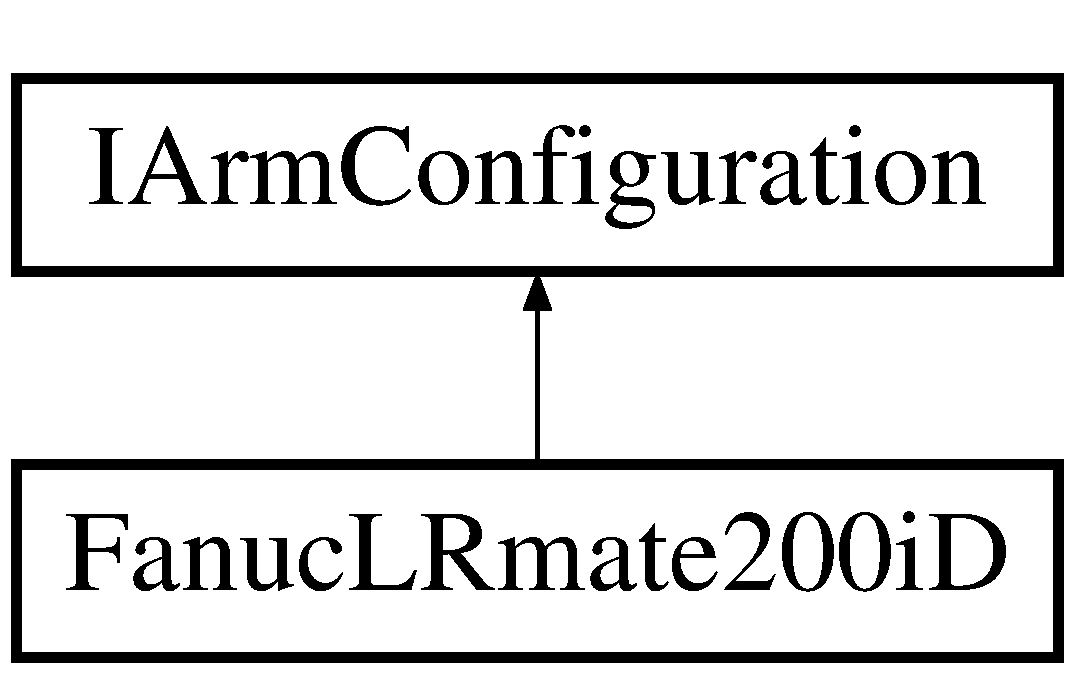
\includegraphics[height=2.000000cm]{classFanucLRmate200iD}
\end{center}
\end{figure}
\subsection*{Public Member Functions}
\begin{DoxyCompactItemize}
\item 
\hyperlink{classFanucLRmate200iD_af584b3786e6932954cdb9c3dc13287fb}{Fanuc\-L\-Rmate200i\-D} ()
\item 
virtual void \hyperlink{classFanucLRmate200iD_a6e8ff8e13061b0c94ce809605218a942}{Configure} (int config, size\-\_\-t size, std\-::vector$<$ double $>$ \&min, std\-::vector$<$ double $>$ \&max)
\end{DoxyCompactItemize}
\subsection*{Additional Inherited Members}


\subsection{Constructor \& Destructor Documentation}
\hypertarget{classFanucLRmate200iD_af584b3786e6932954cdb9c3dc13287fb}{\index{Fanuc\-L\-Rmate200i\-D@{Fanuc\-L\-Rmate200i\-D}!Fanuc\-L\-Rmate200i\-D@{Fanuc\-L\-Rmate200i\-D}}
\index{Fanuc\-L\-Rmate200i\-D@{Fanuc\-L\-Rmate200i\-D}!FanucLRmate200iD@{Fanuc\-L\-Rmate200i\-D}}
\subsubsection[{Fanuc\-L\-Rmate200i\-D}]{\setlength{\rightskip}{0pt plus 5cm}Fanuc\-L\-Rmate200i\-D\-::\-Fanuc\-L\-Rmate200i\-D (
\begin{DoxyParamCaption}
{}
\end{DoxyParamCaption}
)\hspace{0.3cm}{\ttfamily [inline]}}}\label{classFanucLRmate200iD_af584b3786e6932954cdb9c3dc13287fb}


\subsection{Member Function Documentation}
\hypertarget{classFanucLRmate200iD_a6e8ff8e13061b0c94ce809605218a942}{\index{Fanuc\-L\-Rmate200i\-D@{Fanuc\-L\-Rmate200i\-D}!Configure@{Configure}}
\index{Configure@{Configure}!FanucLRmate200iD@{Fanuc\-L\-Rmate200i\-D}}
\subsubsection[{Configure}]{\setlength{\rightskip}{0pt plus 5cm}void Fanuc\-L\-Rmate200i\-D\-::\-Configure (
\begin{DoxyParamCaption}
\item[{int}]{config, }
\item[{size\-\_\-t}]{size, }
\item[{std\-::vector$<$ double $>$ \&}]{min, }
\item[{std\-::vector$<$ double $>$ \&}]{max}
\end{DoxyParamCaption}
)\hspace{0.3cm}{\ttfamily [virtual]}}}\label{classFanucLRmate200iD_a6e8ff8e13061b0c94ce809605218a942}


Reimplemented from \hyperlink{classIArmConfiguration_ab114c4a856a72d43df7ef0fe3c9675e7}{I\-Arm\-Configuration}.



The documentation for this class was generated from the following files\-:\begin{DoxyCompactItemize}
\item 
/usr/local/michalos/nistfanuc\-\_\-ws/src/nist\-\_\-fanuc/include/nist\-\_\-fanuc/\hyperlink{Kinematics_8h}{Kinematics.\-h}\item 
/usr/local/michalos/nistfanuc\-\_\-ws/src/nist\-\_\-fanuc/src/\hyperlink{src_2Kinematics_8cpp}{Kinematics.\-cpp}\end{DoxyCompactItemize}

\hypertarget{classFanucLrMate200idKinematics}{\section{Fanuc\-Lr\-Mate200id\-Kinematics Class Reference}
\label{classFanucLrMate200idKinematics}\index{Fanuc\-Lr\-Mate200id\-Kinematics@{Fanuc\-Lr\-Mate200id\-Kinematics}}
}


{\ttfamily \#include $<$Kinematics.\-h$>$}

Inheritance diagram for Fanuc\-Lr\-Mate200id\-Kinematics\-:\begin{figure}[H]
\begin{center}
\leavevmode
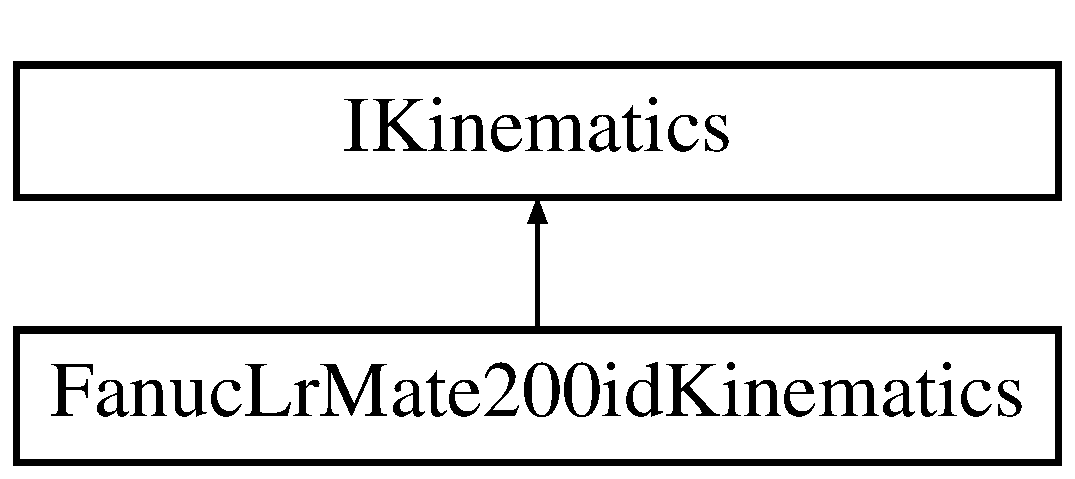
\includegraphics[height=2.000000cm]{classFanucLrMate200idKinematics}
\end{center}
\end{figure}
\subsection*{Public Member Functions}
\begin{DoxyCompactItemize}
\item 
\hyperlink{classFanucLrMate200idKinematics_a4cfa739cb588db9cfaddcb4227662632}{Fanuc\-Lr\-Mate200id\-Kinematics} ()
\item 
virtual \hyperlink{namespaceRCS_aa07e45d8a50e30064283d2b38087f999}{R\-C\-S\-::\-Pose} \hyperlink{classFanucLrMate200idKinematics_a42b44b203b26d356dd9cc7769658138e}{F\-K} (std\-::vector$<$ double $>$ jv)
\begin{DoxyCompactList}\small\item\em F\-K performs the forward kinematics using the joint values of the robot provided. \end{DoxyCompactList}\item 
virtual std\-::vector$<$ double $>$ \hyperlink{classFanucLrMate200idKinematics_a54a3ef5b0e8db49e1ee3362ba2642df6}{I\-K} (\hyperlink{namespaceRCS_aa07e45d8a50e30064283d2b38087f999}{R\-C\-S\-::\-Pose} \&pose, std\-::vector$<$ double $>$ oldjoints)
\begin{DoxyCompactList}\small\item\em I\-K performs the inverse kinematics using the Cartesian pose provided. \end{DoxyCompactList}\item 
virtual size\-\_\-t \hyperlink{classFanucLrMate200idKinematics_a9273cba3818f4ce905f45643d8056eea}{All\-Pose\-To\-Joints} (\hyperlink{namespaceRCS_aa07e45d8a50e30064283d2b38087f999}{R\-C\-S\-::\-Pose} \&pose, std\-::vector$<$ std\-::vector$<$ double $>$ $>$ \&newjoints)
\begin{DoxyCompactList}\small\item\em All\-Pose\-To\-Joints solves the inverse kinematics to find all solutions using the Cartesian pose provided. \end{DoxyCompactList}\item 
virtual std\-::vector$<$ double $>$ \hyperlink{classFanucLrMate200idKinematics_ad7ec485c3eb09775d09512b0e15d3f84}{Nearest\-Joints} (std\-::vector$<$ double $>$ oldjoints, std\-::vector$<$ std\-::vector$<$ double $>$ $>$ \&newjoints)
\begin{DoxyCompactList}\small\item\em Nearest\-Joints finds the joint set that is closest to the old joints. \end{DoxyCompactList}\item 
virtual void \hyperlink{classFanucLrMate200idKinematics_a40dceae1773781d021c86aea16e40da8}{Init} (ros\-::\-Node\-Handle \&nh)
\begin{DoxyCompactList}\small\item\em Initialize kinematics using robot\-\_\-description to fill parameters . \end{DoxyCompactList}\end{DoxyCompactItemize}
\subsection*{Additional Inherited Members}


\subsection{Constructor \& Destructor Documentation}
\hypertarget{classFanucLrMate200idKinematics_a4cfa739cb588db9cfaddcb4227662632}{\index{Fanuc\-Lr\-Mate200id\-Kinematics@{Fanuc\-Lr\-Mate200id\-Kinematics}!Fanuc\-Lr\-Mate200id\-Kinematics@{Fanuc\-Lr\-Mate200id\-Kinematics}}
\index{Fanuc\-Lr\-Mate200id\-Kinematics@{Fanuc\-Lr\-Mate200id\-Kinematics}!FanucLrMate200idKinematics@{Fanuc\-Lr\-Mate200id\-Kinematics}}
\subsubsection[{Fanuc\-Lr\-Mate200id\-Kinematics}]{\setlength{\rightskip}{0pt plus 5cm}Fanuc\-Lr\-Mate200id\-Kinematics\-::\-Fanuc\-Lr\-Mate200id\-Kinematics (
\begin{DoxyParamCaption}
{}
\end{DoxyParamCaption}
)\hspace{0.3cm}{\ttfamily [inline]}}}\label{classFanucLrMate200idKinematics_a4cfa739cb588db9cfaddcb4227662632}


\subsection{Member Function Documentation}
\hypertarget{classFanucLrMate200idKinematics_a9273cba3818f4ce905f45643d8056eea}{\index{Fanuc\-Lr\-Mate200id\-Kinematics@{Fanuc\-Lr\-Mate200id\-Kinematics}!All\-Pose\-To\-Joints@{All\-Pose\-To\-Joints}}
\index{All\-Pose\-To\-Joints@{All\-Pose\-To\-Joints}!FanucLrMate200idKinematics@{Fanuc\-Lr\-Mate200id\-Kinematics}}
\subsubsection[{All\-Pose\-To\-Joints}]{\setlength{\rightskip}{0pt plus 5cm}virtual size\-\_\-t Fanuc\-Lr\-Mate200id\-Kinematics\-::\-All\-Pose\-To\-Joints (
\begin{DoxyParamCaption}
\item[{{\bf R\-C\-S\-::\-Pose} \&}]{pose, }
\item[{std\-::vector$<$ std\-::vector$<$ double $>$ $>$ \&}]{newjoints}
\end{DoxyParamCaption}
)\hspace{0.3cm}{\ttfamily [inline]}, {\ttfamily [virtual]}}}\label{classFanucLrMate200idKinematics_a9273cba3818f4ce905f45643d8056eea}


All\-Pose\-To\-Joints solves the inverse kinematics to find all solutions using the Cartesian pose provided. 


\begin{DoxyParams}{Parameters}
{\em Cartesian} & robot pose of end effector. \\
\hline
{\em vector} & of double vectos to hold all the I\-K joint solutions. \\
\hline
\end{DoxyParams}
\begin{DoxyReturn}{Returns}
number of solutions found. 
\end{DoxyReturn}


Implements \hyperlink{classIKinematics_aeb53bb4b2a1e70a79d5d724e5eb82c10}{I\-Kinematics}.

\hypertarget{classFanucLrMate200idKinematics_a42b44b203b26d356dd9cc7769658138e}{\index{Fanuc\-Lr\-Mate200id\-Kinematics@{Fanuc\-Lr\-Mate200id\-Kinematics}!F\-K@{F\-K}}
\index{F\-K@{F\-K}!FanucLrMate200idKinematics@{Fanuc\-Lr\-Mate200id\-Kinematics}}
\subsubsection[{F\-K}]{\setlength{\rightskip}{0pt plus 5cm}virtual {\bf R\-C\-S\-::\-Pose} Fanuc\-Lr\-Mate200id\-Kinematics\-::\-F\-K (
\begin{DoxyParamCaption}
\item[{std\-::vector$<$ double $>$}]{jv}
\end{DoxyParamCaption}
)\hspace{0.3cm}{\ttfamily [inline]}, {\ttfamily [virtual]}}}\label{classFanucLrMate200idKinematics_a42b44b203b26d356dd9cc7769658138e}


F\-K performs the forward kinematics using the joint values of the robot provided. 


\begin{DoxyParams}{Parameters}
{\em vector} & of all robot joint values in doubles. \\
\hline
\end{DoxyParams}
\begin{DoxyReturn}{Returns}
corresponding Cartesian robot pose of end effector. 
\end{DoxyReturn}


Implements \hyperlink{classIKinematics_abf765053ac39fac5b94ef99e80b17f1b}{I\-Kinematics}.

\hypertarget{classFanucLrMate200idKinematics_a54a3ef5b0e8db49e1ee3362ba2642df6}{\index{Fanuc\-Lr\-Mate200id\-Kinematics@{Fanuc\-Lr\-Mate200id\-Kinematics}!I\-K@{I\-K}}
\index{I\-K@{I\-K}!FanucLrMate200idKinematics@{Fanuc\-Lr\-Mate200id\-Kinematics}}
\subsubsection[{I\-K}]{\setlength{\rightskip}{0pt plus 5cm}virtual std\-::vector$<$double$>$ Fanuc\-Lr\-Mate200id\-Kinematics\-::\-I\-K (
\begin{DoxyParamCaption}
\item[{{\bf R\-C\-S\-::\-Pose} \&}]{pose, }
\item[{std\-::vector$<$ double $>$}]{oldjoints}
\end{DoxyParamCaption}
)\hspace{0.3cm}{\ttfamily [inline]}, {\ttfamily [virtual]}}}\label{classFanucLrMate200idKinematics_a54a3ef5b0e8db49e1ee3362ba2642df6}


I\-K performs the inverse kinematics using the Cartesian pose provided. 


\begin{DoxyParams}{Parameters}
{\em Cartesian} & robot pose of end effector. \\
\hline
{\em optional} & seed joint values to use as best guess for I\-K joint values. \\
\hline
\end{DoxyParams}
\begin{DoxyReturn}{Returns}
vector of all robot joint values in doubles. 
\end{DoxyReturn}


Implements \hyperlink{classIKinematics_ad0715c776a7eb325d2543bc34fa8114f}{I\-Kinematics}.

\hypertarget{classFanucLrMate200idKinematics_a40dceae1773781d021c86aea16e40da8}{\index{Fanuc\-Lr\-Mate200id\-Kinematics@{Fanuc\-Lr\-Mate200id\-Kinematics}!Init@{Init}}
\index{Init@{Init}!FanucLrMate200idKinematics@{Fanuc\-Lr\-Mate200id\-Kinematics}}
\subsubsection[{Init}]{\setlength{\rightskip}{0pt plus 5cm}virtual void Fanuc\-Lr\-Mate200id\-Kinematics\-::\-Init (
\begin{DoxyParamCaption}
\item[{ros\-::\-Node\-Handle \&}]{nh}
\end{DoxyParamCaption}
)\hspace{0.3cm}{\ttfamily [inline]}, {\ttfamily [virtual]}}}\label{classFanucLrMate200idKinematics_a40dceae1773781d021c86aea16e40da8}


Initialize kinematics using robot\-\_\-description to fill parameters . 


\begin{DoxyParams}{Parameters}
{\em nh} & ros node handle of node. \\
\hline
\end{DoxyParams}


Reimplemented from \hyperlink{classIKinematics_aa5c1c9225650b5225f3aa80e06ef1587}{I\-Kinematics}.

\hypertarget{classFanucLrMate200idKinematics_ad7ec485c3eb09775d09512b0e15d3f84}{\index{Fanuc\-Lr\-Mate200id\-Kinematics@{Fanuc\-Lr\-Mate200id\-Kinematics}!Nearest\-Joints@{Nearest\-Joints}}
\index{Nearest\-Joints@{Nearest\-Joints}!FanucLrMate200idKinematics@{Fanuc\-Lr\-Mate200id\-Kinematics}}
\subsubsection[{Nearest\-Joints}]{\setlength{\rightskip}{0pt plus 5cm}virtual std\-::vector$<$double$>$ Fanuc\-Lr\-Mate200id\-Kinematics\-::\-Nearest\-Joints (
\begin{DoxyParamCaption}
\item[{std\-::vector$<$ double $>$}]{oldjoints, }
\item[{std\-::vector$<$ std\-::vector$<$ double $>$ $>$ \&}]{newjoints}
\end{DoxyParamCaption}
)\hspace{0.3cm}{\ttfamily [inline]}, {\ttfamily [virtual]}}}\label{classFanucLrMate200idKinematics_ad7ec485c3eb09775d09512b0e15d3f84}


Nearest\-Joints finds the joint set that is closest to the old joints. 


\begin{DoxyParams}{Parameters}
{\em old} & seed joint values to use as best guess for I\-K joint values. \\
\hline
{\em vector} & of double vectos that holds all the I\-K joint solutions. \\
\hline
\end{DoxyParams}
\begin{DoxyReturn}{Returns}
vector of doubles with closest set to seed joints. 
\end{DoxyReturn}


Implements \hyperlink{classIKinematics_ab74b70ed6ecc53adfc36505b8dd1fef4}{I\-Kinematics}.



The documentation for this class was generated from the following file\-:\begin{DoxyCompactItemize}
\item 
/usr/local/michalos/nistfanuc\-\_\-ws/src/nist\-\_\-fanuc/include/nist\-\_\-fanuc/\hyperlink{Kinematics_8h}{Kinematics.\-h}\end{DoxyCompactItemize}

\hypertarget{classFanucNearestJointsLookup}{\section{Fanuc\-Nearest\-Joints\-Lookup Class Reference}
\label{classFanucNearestJointsLookup}\index{Fanuc\-Nearest\-Joints\-Lookup@{Fanuc\-Nearest\-Joints\-Lookup}}
}


{\ttfamily \#include $<$Demo.\-h$>$}

Inheritance diagram for Fanuc\-Nearest\-Joints\-Lookup\-:\begin{figure}[H]
\begin{center}
\leavevmode
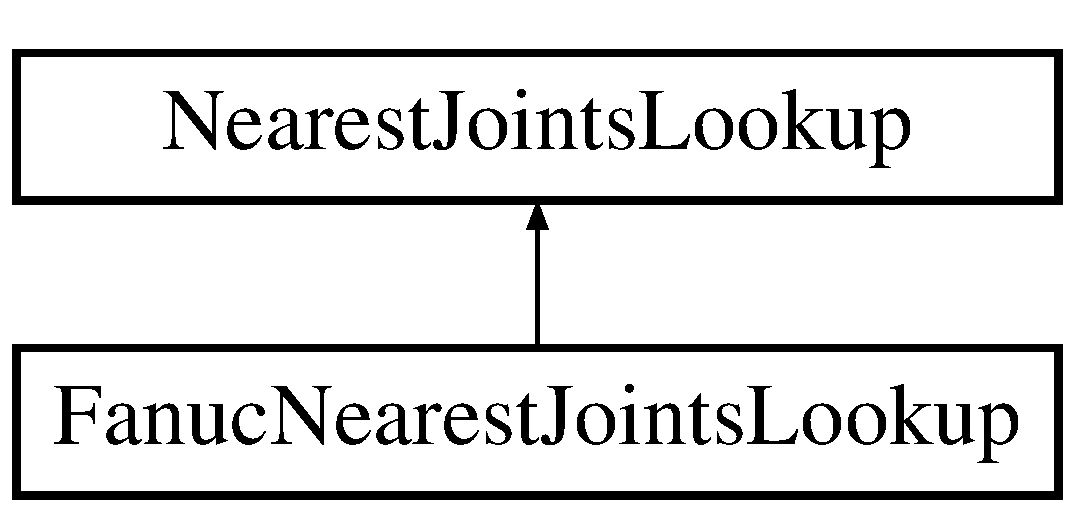
\includegraphics[height=2.000000cm]{classFanucNearestJointsLookup}
\end{center}
\end{figure}
\subsection*{Public Member Functions}
\begin{DoxyCompactItemize}
\item 
\hyperlink{classFanucNearestJointsLookup_a4680c70e79e2cd270317688e4459e78b}{Fanuc\-Nearest\-Joints\-Lookup} (tf\-::\-Pose baseoffset, \hyperlink{Kinematics_8h_aa720b9842c846588baf215581fb9f902}{I\-Kinematics\-Shared\-Ptr} kin)
\item 
virtual void \hyperlink{classFanucNearestJointsLookup_ae543d993aced29b45f60072137edf48a}{Set\-Robot\-Hints} ()
\end{DoxyCompactItemize}
\subsection*{Additional Inherited Members}


\subsection{Constructor \& Destructor Documentation}
\hypertarget{classFanucNearestJointsLookup_a4680c70e79e2cd270317688e4459e78b}{\index{Fanuc\-Nearest\-Joints\-Lookup@{Fanuc\-Nearest\-Joints\-Lookup}!Fanuc\-Nearest\-Joints\-Lookup@{Fanuc\-Nearest\-Joints\-Lookup}}
\index{Fanuc\-Nearest\-Joints\-Lookup@{Fanuc\-Nearest\-Joints\-Lookup}!FanucNearestJointsLookup@{Fanuc\-Nearest\-Joints\-Lookup}}
\subsubsection[{Fanuc\-Nearest\-Joints\-Lookup}]{\setlength{\rightskip}{0pt plus 5cm}Fanuc\-Nearest\-Joints\-Lookup\-::\-Fanuc\-Nearest\-Joints\-Lookup (
\begin{DoxyParamCaption}
\item[{tf\-::\-Pose}]{baseoffset, }
\item[{{\bf I\-Kinematics\-Shared\-Ptr}}]{kin}
\end{DoxyParamCaption}
)\hspace{0.3cm}{\ttfamily [inline]}}}\label{classFanucNearestJointsLookup_a4680c70e79e2cd270317688e4459e78b}


\subsection{Member Function Documentation}
\hypertarget{classFanucNearestJointsLookup_ae543d993aced29b45f60072137edf48a}{\index{Fanuc\-Nearest\-Joints\-Lookup@{Fanuc\-Nearest\-Joints\-Lookup}!Set\-Robot\-Hints@{Set\-Robot\-Hints}}
\index{Set\-Robot\-Hints@{Set\-Robot\-Hints}!FanucNearestJointsLookup@{Fanuc\-Nearest\-Joints\-Lookup}}
\subsubsection[{Set\-Robot\-Hints}]{\setlength{\rightskip}{0pt plus 5cm}void Fanuc\-Nearest\-Joints\-Lookup\-::\-Set\-Robot\-Hints (
\begin{DoxyParamCaption}
{}
\end{DoxyParamCaption}
)\hspace{0.3cm}{\ttfamily [virtual]}}}\label{classFanucNearestJointsLookup_ae543d993aced29b45f60072137edf48a}


Reimplemented from \hyperlink{classNearestJointsLookup_a833cff3f82b12344d2142690e6216340}{Nearest\-Joints\-Lookup}.



The documentation for this class was generated from the following files\-:\begin{DoxyCompactItemize}
\item 
/usr/local/michalos/nistfanuc\-\_\-ws/src/nist\-\_\-fanuc/include/nist\-\_\-fanuc/\hyperlink{Demo_8h}{Demo.\-h}\item 
/usr/local/michalos/nistfanuc\-\_\-ws/src/nist\-\_\-fanuc/src/\hyperlink{Demo_8cpp}{Demo.\-cpp}\end{DoxyCompactItemize}

\hypertarget{classFastKinematics}{\section{Fast\-Kinematics Class Reference}
\label{classFastKinematics}\index{Fast\-Kinematics@{Fast\-Kinematics}}
}


{\ttfamily \#include $<$Kinematics.\-h$>$}

Inheritance diagram for Fast\-Kinematics\-:\begin{figure}[H]
\begin{center}
\leavevmode
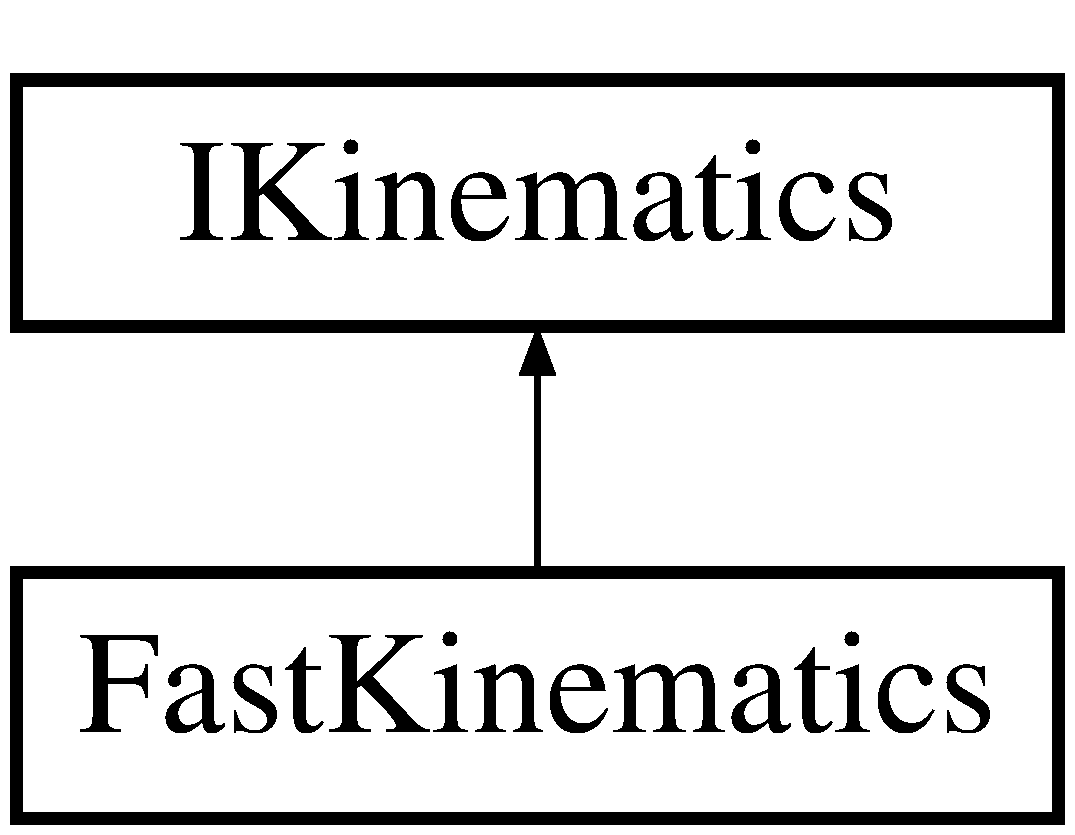
\includegraphics[height=2.000000cm]{classFastKinematics}
\end{center}
\end{figure}
\subsection*{Public Member Functions}
\begin{DoxyCompactItemize}
\item 
virtual \hyperlink{namespaceRCS_aa07e45d8a50e30064283d2b38087f999}{R\-C\-S\-::\-Pose} \hyperlink{classFastKinematics_ad60c8729768b34e653c484a476d471a1}{F\-K} (std\-::vector$<$ double $>$ jv)
\begin{DoxyCompactList}\small\item\em F\-K performs the forward kinematics using the joint values of the robot provided. \end{DoxyCompactList}\item 
virtual size\-\_\-t \hyperlink{classFastKinematics_ab0a88c32e72ad25d48f38b851aabf3fa}{All\-Pose\-To\-Joints} (\hyperlink{namespaceRCS_aa07e45d8a50e30064283d2b38087f999}{R\-C\-S\-::\-Pose} \&pose, std\-::vector$<$ std\-::vector$<$ double $>$$>$ \&joints)
\item 
Eigen\-::\-Vector\-Xd \hyperlink{classFastKinematics_a14981dcd60b8fc6d64e6cf179c1a3ec1}{Convert\-Joints} (std\-::vector$<$ double $>$ v)
\item 
std\-::vector$<$ double $>$ \hyperlink{classFastKinematics_a98431d3915c8b4215992b0fa58af9df3}{Convert\-Joints} (Eigen\-::\-Vector\-Xd ev)
\item 
virtual std\-::vector$<$ double $>$ \hyperlink{classFastKinematics_a8814df8e8bf04cfe6fb48b6e6e8f5c1f}{Nearest\-Joints} (std\-::vector$<$ double $>$ oldjoints, std\-::vector$<$ std\-::vector$<$ double $>$$>$ \&newjoints)
\item 
virtual std\-::vector$<$ double $>$ \hyperlink{classFastKinematics_ad71d66aa03ef1c2d24a190346aa304a1}{I\-K} (\hyperlink{namespaceRCS_aa07e45d8a50e30064283d2b38087f999}{R\-C\-S\-::\-Pose} \&pose, std\-::vector$<$ double $>$ oldjoints)
\begin{DoxyCompactList}\small\item\em I\-K performs the inverse kinematics using the Cartesian pose provided. \end{DoxyCompactList}\item 
virtual std\-::vector$<$ double $>$ \hyperlink{classFastKinematics_a9f9b4b4f95039605a243a85adacd207f}{I\-K} (\hyperlink{namespaceRCS_aa07e45d8a50e30064283d2b38087f999}{R\-C\-S\-::\-Pose} \&pose, std\-::vector$<$ double $>$ minrange, std\-::vector$<$ double $>$ maxrange)
\begin{DoxyCompactList}\small\item\em I\-K performs the inverse kinematics using the Cartesian pose provided. \end{DoxyCompactList}\item 
virtual bool \hyperlink{classFastKinematics_a00652f1e5f1f7bfb9b450576beb7b71f}{Is\-Singular} (\hyperlink{namespaceRCS_aa07e45d8a50e30064283d2b38087f999}{R\-C\-S\-::\-Pose} \&pose, double threshold)
\begin{DoxyCompactList}\small\item\em Returns true if the determinant of the jacobian is near zero. . \end{DoxyCompactList}\item 
virtual void \hyperlink{classFastKinematics_af2de2a0ac3576faffa13dd5357561f78}{Init} (ros\-::\-Node\-Handle \&nh)
\begin{DoxyCompactList}\small\item\em Initialize kinematics using robot\-\_\-description to fill parameters . \end{DoxyCompactList}\item 
void \hyperlink{classFastKinematics_af9fd72624869d472acc17bfb14998b50}{Verify\-Limits} (std\-::vector$<$ double $>$ joints)
\item 
virtual std\-::vector$<$ double $>$ \hyperlink{classFastKinematics_a811d12eb6c664d72d4ae5a685d219185}{Find\-Bounded\-Solution} (std\-::vector$<$ std\-::vector$<$ double $>$$>$ \&solutions, std\-::vector$<$ double $>$ \&min, std\-::vector$<$ double $>$ \&max)
\end{DoxyCompactItemize}
\subsection*{Additional Inherited Members}


\subsection{Member Function Documentation}
\hypertarget{classFastKinematics_ab0a88c32e72ad25d48f38b851aabf3fa}{\index{Fast\-Kinematics@{Fast\-Kinematics}!All\-Pose\-To\-Joints@{All\-Pose\-To\-Joints}}
\index{All\-Pose\-To\-Joints@{All\-Pose\-To\-Joints}!FastKinematics@{Fast\-Kinematics}}
\subsubsection[{All\-Pose\-To\-Joints}]{\setlength{\rightskip}{0pt plus 5cm}virtual size\-\_\-t Fast\-Kinematics\-::\-All\-Pose\-To\-Joints (
\begin{DoxyParamCaption}
\item[{{\bf R\-C\-S\-::\-Pose} \&}]{pose, }
\item[{std\-::vector$<$ std\-::vector$<$ double $>$$>$ \&}]{joints}
\end{DoxyParamCaption}
)\hspace{0.3cm}{\ttfamily [inline]}, {\ttfamily [virtual]}}}\label{classFastKinematics_ab0a88c32e72ad25d48f38b851aabf3fa}
\hypertarget{classFastKinematics_a14981dcd60b8fc6d64e6cf179c1a3ec1}{\index{Fast\-Kinematics@{Fast\-Kinematics}!Convert\-Joints@{Convert\-Joints}}
\index{Convert\-Joints@{Convert\-Joints}!FastKinematics@{Fast\-Kinematics}}
\subsubsection[{Convert\-Joints}]{\setlength{\rightskip}{0pt plus 5cm}Eigen\-::\-Vector\-Xd Fast\-Kinematics\-::\-Convert\-Joints (
\begin{DoxyParamCaption}
\item[{std\-::vector$<$ double $>$}]{v}
\end{DoxyParamCaption}
)\hspace{0.3cm}{\ttfamily [inline]}}}\label{classFastKinematics_a14981dcd60b8fc6d64e6cf179c1a3ec1}
\hypertarget{classFastKinematics_a98431d3915c8b4215992b0fa58af9df3}{\index{Fast\-Kinematics@{Fast\-Kinematics}!Convert\-Joints@{Convert\-Joints}}
\index{Convert\-Joints@{Convert\-Joints}!FastKinematics@{Fast\-Kinematics}}
\subsubsection[{Convert\-Joints}]{\setlength{\rightskip}{0pt plus 5cm}std\-::vector$<$double$>$ Fast\-Kinematics\-::\-Convert\-Joints (
\begin{DoxyParamCaption}
\item[{Eigen\-::\-Vector\-Xd}]{ev}
\end{DoxyParamCaption}
)\hspace{0.3cm}{\ttfamily [inline]}}}\label{classFastKinematics_a98431d3915c8b4215992b0fa58af9df3}
\hypertarget{classFastKinematics_a811d12eb6c664d72d4ae5a685d219185}{\index{Fast\-Kinematics@{Fast\-Kinematics}!Find\-Bounded\-Solution@{Find\-Bounded\-Solution}}
\index{Find\-Bounded\-Solution@{Find\-Bounded\-Solution}!FastKinematics@{Fast\-Kinematics}}
\subsubsection[{Find\-Bounded\-Solution}]{\setlength{\rightskip}{0pt plus 5cm}std\-::vector$<$ double $>$ Fast\-Kinematics\-::\-Find\-Bounded\-Solution (
\begin{DoxyParamCaption}
\item[{std\-::vector$<$ std\-::vector$<$ double $>$$>$ \&}]{solutions, }
\item[{std\-::vector$<$ double $>$ \&}]{min, }
\item[{std\-::vector$<$ double $>$ \&}]{max}
\end{DoxyParamCaption}
)\hspace{0.3cm}{\ttfamily [virtual]}}}\label{classFastKinematics_a811d12eb6c664d72d4ae5a685d219185}


Reimplemented from \hyperlink{classIKinematics_ab792f1f7ee1f2a34cb33eae02f1a91f9}{I\-Kinematics}.

\hypertarget{classFastKinematics_ad60c8729768b34e653c484a476d471a1}{\index{Fast\-Kinematics@{Fast\-Kinematics}!F\-K@{F\-K}}
\index{F\-K@{F\-K}!FastKinematics@{Fast\-Kinematics}}
\subsubsection[{F\-K}]{\setlength{\rightskip}{0pt plus 5cm}virtual {\bf R\-C\-S\-::\-Pose} Fast\-Kinematics\-::\-F\-K (
\begin{DoxyParamCaption}
\item[{std\-::vector$<$ double $>$}]{jv}
\end{DoxyParamCaption}
)\hspace{0.3cm}{\ttfamily [inline]}, {\ttfamily [virtual]}}}\label{classFastKinematics_ad60c8729768b34e653c484a476d471a1}


F\-K performs the forward kinematics using the joint values of the robot provided. 


\begin{DoxyParams}{Parameters}
{\em vector} & of all robot joint values in doubles. \\
\hline
\end{DoxyParams}
\begin{DoxyReturn}{Returns}
corresponding Cartesian robot pose of end effector. 
\end{DoxyReturn}


Implements \hyperlink{classIKinematics_abf765053ac39fac5b94ef99e80b17f1b}{I\-Kinematics}.

\hypertarget{classFastKinematics_ad71d66aa03ef1c2d24a190346aa304a1}{\index{Fast\-Kinematics@{Fast\-Kinematics}!I\-K@{I\-K}}
\index{I\-K@{I\-K}!FastKinematics@{Fast\-Kinematics}}
\subsubsection[{I\-K}]{\setlength{\rightskip}{0pt plus 5cm}virtual std\-::vector$<$double$>$ Fast\-Kinematics\-::\-I\-K (
\begin{DoxyParamCaption}
\item[{{\bf R\-C\-S\-::\-Pose} \&}]{pose, }
\item[{std\-::vector$<$ double $>$}]{oldjoints}
\end{DoxyParamCaption}
)\hspace{0.3cm}{\ttfamily [inline]}, {\ttfamily [virtual]}}}\label{classFastKinematics_ad71d66aa03ef1c2d24a190346aa304a1}


I\-K performs the inverse kinematics using the Cartesian pose provided. 


\begin{DoxyParams}{Parameters}
{\em Cartesian} & robot pose of end effector. \\
\hline
{\em optional} & seed joint values to use as best guess for I\-K joint values. \\
\hline
\end{DoxyParams}
\begin{DoxyReturn}{Returns}
vector of all robot joint values in doubles. 
\end{DoxyReturn}


Implements \hyperlink{classIKinematics_ad0715c776a7eb325d2543bc34fa8114f}{I\-Kinematics}.

\hypertarget{classFastKinematics_a9f9b4b4f95039605a243a85adacd207f}{\index{Fast\-Kinematics@{Fast\-Kinematics}!I\-K@{I\-K}}
\index{I\-K@{I\-K}!FastKinematics@{Fast\-Kinematics}}
\subsubsection[{I\-K}]{\setlength{\rightskip}{0pt plus 5cm}virtual std\-::vector$<$double$>$ Fast\-Kinematics\-::\-I\-K (
\begin{DoxyParamCaption}
\item[{{\bf R\-C\-S\-::\-Pose} \&}]{pose, }
\item[{std\-::vector$<$ double $>$}]{minrange, }
\item[{std\-::vector$<$ double $>$}]{maxrange}
\end{DoxyParamCaption}
)\hspace{0.3cm}{\ttfamily [inline]}, {\ttfamily [virtual]}}}\label{classFastKinematics_a9f9b4b4f95039605a243a85adacd207f}


I\-K performs the inverse kinematics using the Cartesian pose provided. 


\begin{DoxyParams}{Parameters}
{\em Cartesian} & robot pose of end effector. \\
\hline
{\em optional} & seed joint values to use as best guess for I\-K joint values. \\
\hline
\end{DoxyParams}
\begin{DoxyReturn}{Returns}
vector of all robot joint values in doubles. 
\end{DoxyReturn}


Reimplemented from \hyperlink{classIKinematics_a2b5554a09667fa0b985f3954306841ea}{I\-Kinematics}.

\hypertarget{classFastKinematics_af2de2a0ac3576faffa13dd5357561f78}{\index{Fast\-Kinematics@{Fast\-Kinematics}!Init@{Init}}
\index{Init@{Init}!FastKinematics@{Fast\-Kinematics}}
\subsubsection[{Init}]{\setlength{\rightskip}{0pt plus 5cm}virtual void Fast\-Kinematics\-::\-Init (
\begin{DoxyParamCaption}
\item[{ros\-::\-Node\-Handle \&}]{nh}
\end{DoxyParamCaption}
)\hspace{0.3cm}{\ttfamily [inline]}, {\ttfamily [virtual]}}}\label{classFastKinematics_af2de2a0ac3576faffa13dd5357561f78}


Initialize kinematics using robot\-\_\-description to fill parameters . 


\begin{DoxyParams}{Parameters}
{\em nh} & ros node handle of node. \\
\hline
\end{DoxyParams}


Reimplemented from \hyperlink{classIKinematics_aa5c1c9225650b5225f3aa80e06ef1587}{I\-Kinematics}.

\hypertarget{classFastKinematics_a00652f1e5f1f7bfb9b450576beb7b71f}{\index{Fast\-Kinematics@{Fast\-Kinematics}!Is\-Singular@{Is\-Singular}}
\index{Is\-Singular@{Is\-Singular}!FastKinematics@{Fast\-Kinematics}}
\subsubsection[{Is\-Singular}]{\setlength{\rightskip}{0pt plus 5cm}virtual bool Fast\-Kinematics\-::\-Is\-Singular (
\begin{DoxyParamCaption}
\item[{{\bf R\-C\-S\-::\-Pose} \&}]{pose, }
\item[{double}]{threshold}
\end{DoxyParamCaption}
)\hspace{0.3cm}{\ttfamily [inline]}, {\ttfamily [virtual]}}}\label{classFastKinematics_a00652f1e5f1f7bfb9b450576beb7b71f}


Returns true if the determinant of the jacobian is near zero. . 


\begin{DoxyParams}{Parameters}
{\em groupname} & name of chained joints in robot model. \\
\hline
{\em eelinkname} & name of end effector joint in robot model. \\
\hline
\end{DoxyParams}


Reimplemented from \hyperlink{classIKinematics_aac7d4f55bbd9228af0a7b733f857fcab}{I\-Kinematics}.

\hypertarget{classFastKinematics_a8814df8e8bf04cfe6fb48b6e6e8f5c1f}{\index{Fast\-Kinematics@{Fast\-Kinematics}!Nearest\-Joints@{Nearest\-Joints}}
\index{Nearest\-Joints@{Nearest\-Joints}!FastKinematics@{Fast\-Kinematics}}
\subsubsection[{Nearest\-Joints}]{\setlength{\rightskip}{0pt plus 5cm}virtual std\-::vector$<$double$>$ Fast\-Kinematics\-::\-Nearest\-Joints (
\begin{DoxyParamCaption}
\item[{std\-::vector$<$ double $>$}]{oldjoints, }
\item[{std\-::vector$<$ std\-::vector$<$ double $>$$>$ \&}]{newjoints}
\end{DoxyParamCaption}
)\hspace{0.3cm}{\ttfamily [inline]}, {\ttfamily [virtual]}}}\label{classFastKinematics_a8814df8e8bf04cfe6fb48b6e6e8f5c1f}
\hypertarget{classFastKinematics_af9fd72624869d472acc17bfb14998b50}{\index{Fast\-Kinematics@{Fast\-Kinematics}!Verify\-Limits@{Verify\-Limits}}
\index{Verify\-Limits@{Verify\-Limits}!FastKinematics@{Fast\-Kinematics}}
\subsubsection[{Verify\-Limits}]{\setlength{\rightskip}{0pt plus 5cm}void Fast\-Kinematics\-::\-Verify\-Limits (
\begin{DoxyParamCaption}
\item[{std\-::vector$<$ double $>$}]{joints}
\end{DoxyParamCaption}
)\hspace{0.3cm}{\ttfamily [inline]}}}\label{classFastKinematics_af9fd72624869d472acc17bfb14998b50}


The documentation for this class was generated from the following files\-:\begin{DoxyCompactItemize}
\item 
/usr/local/michalos/nistfanuc\-\_\-ws/src/nist\-\_\-fanuc/include/nist\-\_\-fanuc/\hyperlink{Kinematics_8h}{Kinematics.\-h}\item 
/usr/local/michalos/nistfanuc\-\_\-ws/src/nist\-\_\-fanuc/src/\hyperlink{src_2Kinematics_8cpp}{Kinematics.\-cpp}\end{DoxyCompactItemize}

\hypertarget{classGripperInterface}{\section{Gripper\-Interface Class Reference}
\label{classGripperInterface}\index{Gripper\-Interface@{Gripper\-Interface}}
}


{\ttfamily \#include $<$Gripper.\-h$>$}

\subsection*{Public Member Functions}
\begin{DoxyCompactItemize}
\item 
\hyperlink{classGripperInterface_a029b0f601974702f9e5eabaebc025f0f}{Gripper\-Interface} ()
\item 
void \hyperlink{classGripperInterface_aa08d8e1ef6d63f4e50a0d7359b800fe8}{init} (ros\-::\-Node\-Handle \&nh, std\-::string \hyperlink{classGripperInterface_af8175e1d6b1bd3d25a285cc2063bfae3}{prefix}, bool b\-Publish=false)
\item 
std\-::vector$<$ std\-::string $>$ \hyperlink{classGripperInterface_ab65fbcdfc969ba5d01c9f5d4256f0981}{Joint\-Names} ()
\item 
\hyperlink{RCS_8h_aa4adb93a26caa4dacba9c9614e283245}{sensor\-\_\-msgs\-::\-Joint\-State} \hyperlink{classGripperInterface_a4e880e17fb0e340d13ec474c5b1e242b}{close\-Setup} ()
\item 
void \hyperlink{classGripperInterface_a3a5a0f98239a390004780a546da0964d}{close} ()
\item 
void \hyperlink{classGripperInterface_abc58ac3146134b048f27dd41214c90e8}{publish\-\_\-jointstate} ()
\item 
\hyperlink{RCS_8h_aa4adb93a26caa4dacba9c9614e283245}{sensor\-\_\-msgs\-::\-Joint\-State} \hyperlink{classGripperInterface_a0b48f2f499ea51aeddbac9cef14c41da}{open\-Setup} ()
\item 
void \hyperlink{classGripperInterface_acd38ac748d96a2831cebd11b00421ee0}{open} ()
\item 
\hyperlink{RCS_8h_aa4adb93a26caa4dacba9c9614e283245}{sensor\-\_\-msgs\-::\-Joint\-State} \hyperlink{classGripperInterface_a716fca65b73e2eab7be9d0ad09a01f75}{set\-Position} (double position)
\end{DoxyCompactItemize}
\subsection*{Public Attributes}
\begin{DoxyCompactItemize}
\item 
ros\-::\-Publisher \hyperlink{classGripperInterface_a1bd391402e2051e744063289506b6247}{joint\-\_\-pub}
\item 
std\-::vector$<$ std\-::string $>$ \hyperlink{classGripperInterface_a2175efb34e767fddbeb230b4bd76d5d4}{joint\-\_\-names}
\item 
const double \hyperlink{classGripperInterface_ab3d004505c5be0bb95b5e0b4746a6119}{degree} = M\-\_\-\-P\-I / 180
\item 
\hyperlink{RCS_8h_aa4adb93a26caa4dacba9c9614e283245}{sensor\-\_\-msgs\-::\-Joint\-State} \hyperlink{classGripperInterface_a8c141d69172982d454e4d8bc11a77645}{joint\-\_\-state}
\item 
std\-::string \hyperlink{classGripperInterface_af8175e1d6b1bd3d25a285cc2063bfae3}{prefix}
\end{DoxyCompactItemize}


\subsection{Constructor \& Destructor Documentation}
\hypertarget{classGripperInterface_a029b0f601974702f9e5eabaebc025f0f}{\index{Gripper\-Interface@{Gripper\-Interface}!Gripper\-Interface@{Gripper\-Interface}}
\index{Gripper\-Interface@{Gripper\-Interface}!GripperInterface@{Gripper\-Interface}}
\subsubsection[{Gripper\-Interface}]{\setlength{\rightskip}{0pt plus 5cm}Gripper\-Interface\-::\-Gripper\-Interface (
\begin{DoxyParamCaption}
{}
\end{DoxyParamCaption}
)\hspace{0.3cm}{\ttfamily [inline]}}}\label{classGripperInterface_a029b0f601974702f9e5eabaebc025f0f}


\subsection{Member Function Documentation}
\hypertarget{classGripperInterface_a3a5a0f98239a390004780a546da0964d}{\index{Gripper\-Interface@{Gripper\-Interface}!close@{close}}
\index{close@{close}!GripperInterface@{Gripper\-Interface}}
\subsubsection[{close}]{\setlength{\rightskip}{0pt plus 5cm}void Gripper\-Interface\-::close (
\begin{DoxyParamCaption}
{}
\end{DoxyParamCaption}
)\hspace{0.3cm}{\ttfamily [inline]}}}\label{classGripperInterface_a3a5a0f98239a390004780a546da0964d}
\hypertarget{classGripperInterface_a4e880e17fb0e340d13ec474c5b1e242b}{\index{Gripper\-Interface@{Gripper\-Interface}!close\-Setup@{close\-Setup}}
\index{close\-Setup@{close\-Setup}!GripperInterface@{Gripper\-Interface}}
\subsubsection[{close\-Setup}]{\setlength{\rightskip}{0pt plus 5cm}{\bf sensor\-\_\-msgs\-::\-Joint\-State} Gripper\-Interface\-::close\-Setup (
\begin{DoxyParamCaption}
{}
\end{DoxyParamCaption}
)\hspace{0.3cm}{\ttfamily [inline]}}}\label{classGripperInterface_a4e880e17fb0e340d13ec474c5b1e242b}
\hypertarget{classGripperInterface_aa08d8e1ef6d63f4e50a0d7359b800fe8}{\index{Gripper\-Interface@{Gripper\-Interface}!init@{init}}
\index{init@{init}!GripperInterface@{Gripper\-Interface}}
\subsubsection[{init}]{\setlength{\rightskip}{0pt plus 5cm}void Gripper\-Interface\-::init (
\begin{DoxyParamCaption}
\item[{ros\-::\-Node\-Handle \&}]{nh, }
\item[{std\-::string}]{prefix, }
\item[{bool}]{b\-Publish = {\ttfamily false}}
\end{DoxyParamCaption}
)\hspace{0.3cm}{\ttfamily [inline]}}}\label{classGripperInterface_aa08d8e1ef6d63f4e50a0d7359b800fe8}
\hypertarget{classGripperInterface_ab65fbcdfc969ba5d01c9f5d4256f0981}{\index{Gripper\-Interface@{Gripper\-Interface}!Joint\-Names@{Joint\-Names}}
\index{Joint\-Names@{Joint\-Names}!GripperInterface@{Gripper\-Interface}}
\subsubsection[{Joint\-Names}]{\setlength{\rightskip}{0pt plus 5cm}std\-::vector$<$std\-::string$>$ Gripper\-Interface\-::\-Joint\-Names (
\begin{DoxyParamCaption}
{}
\end{DoxyParamCaption}
)\hspace{0.3cm}{\ttfamily [inline]}}}\label{classGripperInterface_ab65fbcdfc969ba5d01c9f5d4256f0981}
\hypertarget{classGripperInterface_acd38ac748d96a2831cebd11b00421ee0}{\index{Gripper\-Interface@{Gripper\-Interface}!open@{open}}
\index{open@{open}!GripperInterface@{Gripper\-Interface}}
\subsubsection[{open}]{\setlength{\rightskip}{0pt plus 5cm}void Gripper\-Interface\-::open (
\begin{DoxyParamCaption}
{}
\end{DoxyParamCaption}
)\hspace{0.3cm}{\ttfamily [inline]}}}\label{classGripperInterface_acd38ac748d96a2831cebd11b00421ee0}
\hypertarget{classGripperInterface_a0b48f2f499ea51aeddbac9cef14c41da}{\index{Gripper\-Interface@{Gripper\-Interface}!open\-Setup@{open\-Setup}}
\index{open\-Setup@{open\-Setup}!GripperInterface@{Gripper\-Interface}}
\subsubsection[{open\-Setup}]{\setlength{\rightskip}{0pt plus 5cm}{\bf sensor\-\_\-msgs\-::\-Joint\-State} Gripper\-Interface\-::open\-Setup (
\begin{DoxyParamCaption}
{}
\end{DoxyParamCaption}
)\hspace{0.3cm}{\ttfamily [inline]}}}\label{classGripperInterface_a0b48f2f499ea51aeddbac9cef14c41da}
\hypertarget{classGripperInterface_abc58ac3146134b048f27dd41214c90e8}{\index{Gripper\-Interface@{Gripper\-Interface}!publish\-\_\-jointstate@{publish\-\_\-jointstate}}
\index{publish\-\_\-jointstate@{publish\-\_\-jointstate}!GripperInterface@{Gripper\-Interface}}
\subsubsection[{publish\-\_\-jointstate}]{\setlength{\rightskip}{0pt plus 5cm}void Gripper\-Interface\-::publish\-\_\-jointstate (
\begin{DoxyParamCaption}
{}
\end{DoxyParamCaption}
)\hspace{0.3cm}{\ttfamily [inline]}}}\label{classGripperInterface_abc58ac3146134b048f27dd41214c90e8}
\hypertarget{classGripperInterface_a716fca65b73e2eab7be9d0ad09a01f75}{\index{Gripper\-Interface@{Gripper\-Interface}!set\-Position@{set\-Position}}
\index{set\-Position@{set\-Position}!GripperInterface@{Gripper\-Interface}}
\subsubsection[{set\-Position}]{\setlength{\rightskip}{0pt plus 5cm}{\bf sensor\-\_\-msgs\-::\-Joint\-State} Gripper\-Interface\-::set\-Position (
\begin{DoxyParamCaption}
\item[{double}]{position}
\end{DoxyParamCaption}
)\hspace{0.3cm}{\ttfamily [inline]}}}\label{classGripperInterface_a716fca65b73e2eab7be9d0ad09a01f75}


\subsection{Member Data Documentation}
\hypertarget{classGripperInterface_ab3d004505c5be0bb95b5e0b4746a6119}{\index{Gripper\-Interface@{Gripper\-Interface}!degree@{degree}}
\index{degree@{degree}!GripperInterface@{Gripper\-Interface}}
\subsubsection[{degree}]{\setlength{\rightskip}{0pt plus 5cm}const double Gripper\-Interface\-::degree = M\-\_\-\-P\-I / 180}}\label{classGripperInterface_ab3d004505c5be0bb95b5e0b4746a6119}
\hypertarget{classGripperInterface_a2175efb34e767fddbeb230b4bd76d5d4}{\index{Gripper\-Interface@{Gripper\-Interface}!joint\-\_\-names@{joint\-\_\-names}}
\index{joint\-\_\-names@{joint\-\_\-names}!GripperInterface@{Gripper\-Interface}}
\subsubsection[{joint\-\_\-names}]{\setlength{\rightskip}{0pt plus 5cm}std\-::vector$<$std\-::string$>$ Gripper\-Interface\-::joint\-\_\-names}}\label{classGripperInterface_a2175efb34e767fddbeb230b4bd76d5d4}
\hypertarget{classGripperInterface_a1bd391402e2051e744063289506b6247}{\index{Gripper\-Interface@{Gripper\-Interface}!joint\-\_\-pub@{joint\-\_\-pub}}
\index{joint\-\_\-pub@{joint\-\_\-pub}!GripperInterface@{Gripper\-Interface}}
\subsubsection[{joint\-\_\-pub}]{\setlength{\rightskip}{0pt plus 5cm}ros\-::\-Publisher Gripper\-Interface\-::joint\-\_\-pub}}\label{classGripperInterface_a1bd391402e2051e744063289506b6247}
\hypertarget{classGripperInterface_a8c141d69172982d454e4d8bc11a77645}{\index{Gripper\-Interface@{Gripper\-Interface}!joint\-\_\-state@{joint\-\_\-state}}
\index{joint\-\_\-state@{joint\-\_\-state}!GripperInterface@{Gripper\-Interface}}
\subsubsection[{joint\-\_\-state}]{\setlength{\rightskip}{0pt plus 5cm}{\bf sensor\-\_\-msgs\-::\-Joint\-State} Gripper\-Interface\-::joint\-\_\-state}}\label{classGripperInterface_a8c141d69172982d454e4d8bc11a77645}
\hypertarget{classGripperInterface_af8175e1d6b1bd3d25a285cc2063bfae3}{\index{Gripper\-Interface@{Gripper\-Interface}!prefix@{prefix}}
\index{prefix@{prefix}!GripperInterface@{Gripper\-Interface}}
\subsubsection[{prefix}]{\setlength{\rightskip}{0pt plus 5cm}std\-::string Gripper\-Interface\-::prefix}}\label{classGripperInterface_af8175e1d6b1bd3d25a285cc2063bfae3}


The documentation for this class was generated from the following file\-:\begin{DoxyCompactItemize}
\item 
/usr/local/michalos/nistfanuc\-\_\-ws/src/nist\-\_\-fanuc/include/nist\-\_\-fanuc/\hyperlink{Gripper_8h}{Gripper.\-h}\end{DoxyCompactItemize}

\hypertarget{classIArmConfiguration}{\section{I\-Arm\-Configuration Class Reference}
\label{classIArmConfiguration}\index{I\-Arm\-Configuration@{I\-Arm\-Configuration}}
}


{\ttfamily \#include $<$Kinematics.\-h$>$}

Inheritance diagram for I\-Arm\-Configuration\-:\begin{figure}[H]
\begin{center}
\leavevmode
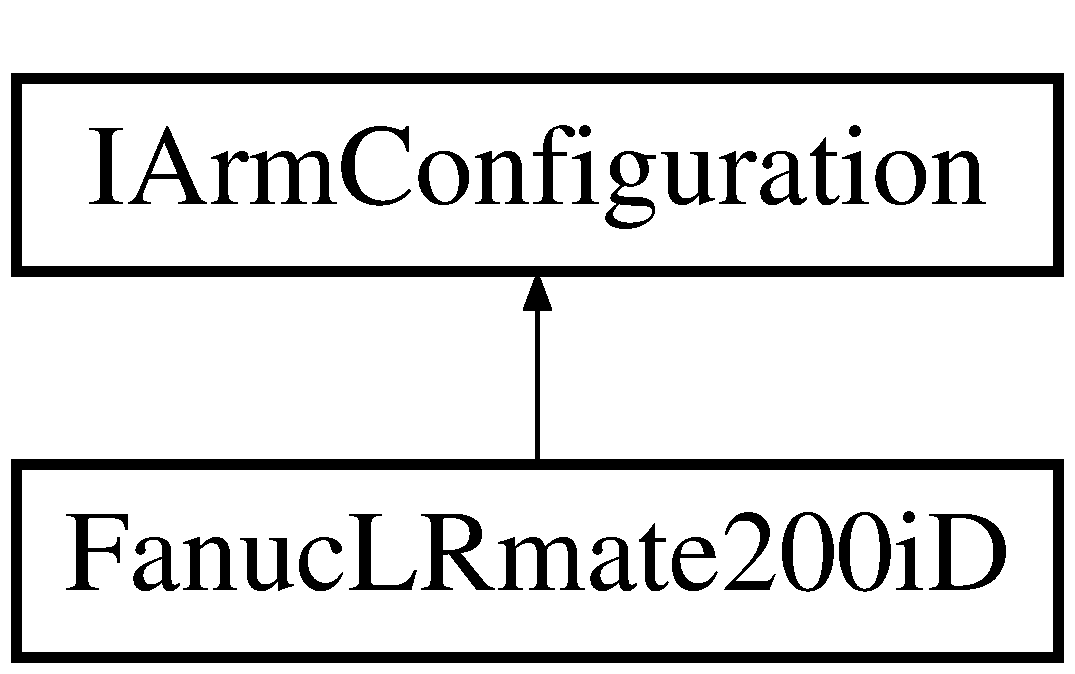
\includegraphics[height=2.000000cm]{classIArmConfiguration}
\end{center}
\end{figure}
\subsection*{Public Member Functions}
\begin{DoxyCompactItemize}
\item 
\hyperlink{classIArmConfiguration_a9422c85c85d341b821f2b121aafea7f6}{I\-Arm\-Configuration} ()
\item 
virtual void \hyperlink{classIArmConfiguration_ab114c4a856a72d43df7ef0fe3c9675e7}{Configure} (int config, size\-\_\-t size, std\-::vector$<$ double $>$ \&min, std\-::vector$<$ double $>$ \&max)
\item 
void \hyperlink{classIArmConfiguration_adc675690b8a93fc0c89af315f8a755df}{Range} (std\-::vector$<$ double $>$ \&min, std\-::vector$<$ double $>$ \&max)
\end{DoxyCompactItemize}
\subsection*{Static Public Attributes}
\begin{DoxyCompactItemize}
\item 
static const int \hyperlink{classIArmConfiguration_a350358b5db8e596cfe0a807e86606f73}{B\-A\-S\-E\-\_\-\-F\-L\-I\-P} = 0x01
\item 
static const int \hyperlink{classIArmConfiguration_a54057fc8c00daa9cf44af3cf3e89ba47}{A\-R\-M\-\_\-\-B\-A\-C\-K\-W\-A\-R\-D} = 0x02
\item 
static const int \hyperlink{classIArmConfiguration_a669c41de4b34b0c56acaabd46a43dadb}{S\-H\-O\-U\-L\-D\-E\-R\-\_\-\-R\-I\-G\-H\-T} = 0x040
\item 
static const int \hyperlink{classIArmConfiguration_ad715705eeb8c3835f2e0b749e4e8e043}{S\-H\-O\-U\-L\-D\-E\-R\-\_\-\-D\-O\-W\-N} = 0x04
\item 
static const int \hyperlink{classIArmConfiguration_ad933d24036398d6887f6b208866948eb}{S\-H\-O\-U\-L\-D\-E\-R\-\_\-\-U\-P} = 0x040
\item 
static const int \hyperlink{classIArmConfiguration_ae27619e20b7e7480cdbfc20062bb251b}{E\-L\-B\-O\-W\-\_\-\-D\-O\-W\-N} = 0x08
\item 
static const int \hyperlink{classIArmConfiguration_a408617f0f4302aad13dc8cb43e377d50}{E\-L\-B\-O\-W\-\_\-\-U\-P} = 0x080
\item 
static const int \hyperlink{classIArmConfiguration_a4c640de35c1fc5c61b5dc950588089d7}{F\-O\-R\-E\-A\-R\-M\-\_\-\-U\-P} = 0x10
\item 
static const int \hyperlink{classIArmConfiguration_a4243f9146bc20c3ce2c8796c04852cb4}{F\-O\-R\-E\-A\-R\-M\-\_\-\-D\-O\-W\-N} = 0x100
\item 
static const int \hyperlink{classIArmConfiguration_ae2cf37e0ff2e11888bcf97a5bf9ca824}{W\-R\-I\-S\-T\-\_\-\-N\-O\-R\-M\-A\-L} = 0x200
\item 
static const int \hyperlink{classIArmConfiguration_a80649ead98210dbc5fe8d9c28f1f4f98}{W\-R\-I\-S\-T\-\_\-\-F\-L\-I\-P} = 0x400
\item 
static const int \hyperlink{classIArmConfiguration_a02c7db5fe651e5e14928c214dfe53da6}{S\-I\-N\-G\-U\-L\-A\-R} = -\/1
\end{DoxyCompactItemize}
\subsection*{Protected Attributes}
\begin{DoxyCompactItemize}
\item 
int \hyperlink{classIArmConfiguration_a0075e845267a9821acd152ce4866e66c}{\-\_\-config}
\item 
size\-\_\-t \hyperlink{classIArmConfiguration_a58e9669a13e5409691f4cc5511bd26b1}{\-\_\-size}
\item 
std\-::vector$<$ double $>$ \hyperlink{classIArmConfiguration_ae918d115cd3bb8702dee12799666c630}{\-\_\-min}
\item 
std\-::vector$<$ double $>$ \hyperlink{classIArmConfiguration_a3103e1f2fff69e56a46e3277e02649a9}{\-\_\-max}
\item 
bool \hyperlink{classIArmConfiguration_ab85f30ca3611448a2cc93583a408d342}{b\-Config}
\end{DoxyCompactItemize}


\subsection{Constructor \& Destructor Documentation}
\hypertarget{classIArmConfiguration_a9422c85c85d341b821f2b121aafea7f6}{\index{I\-Arm\-Configuration@{I\-Arm\-Configuration}!I\-Arm\-Configuration@{I\-Arm\-Configuration}}
\index{I\-Arm\-Configuration@{I\-Arm\-Configuration}!IArmConfiguration@{I\-Arm\-Configuration}}
\subsubsection[{I\-Arm\-Configuration}]{\setlength{\rightskip}{0pt plus 5cm}I\-Arm\-Configuration\-::\-I\-Arm\-Configuration (
\begin{DoxyParamCaption}
{}
\end{DoxyParamCaption}
)\hspace{0.3cm}{\ttfamily [inline]}}}\label{classIArmConfiguration_a9422c85c85d341b821f2b121aafea7f6}


\subsection{Member Function Documentation}
\hypertarget{classIArmConfiguration_ab114c4a856a72d43df7ef0fe3c9675e7}{\index{I\-Arm\-Configuration@{I\-Arm\-Configuration}!Configure@{Configure}}
\index{Configure@{Configure}!IArmConfiguration@{I\-Arm\-Configuration}}
\subsubsection[{Configure}]{\setlength{\rightskip}{0pt plus 5cm}virtual void I\-Arm\-Configuration\-::\-Configure (
\begin{DoxyParamCaption}
\item[{int}]{config, }
\item[{size\-\_\-t}]{size, }
\item[{std\-::vector$<$ double $>$ \&}]{min, }
\item[{std\-::vector$<$ double $>$ \&}]{max}
\end{DoxyParamCaption}
)\hspace{0.3cm}{\ttfamily [inline]}, {\ttfamily [virtual]}}}\label{classIArmConfiguration_ab114c4a856a72d43df7ef0fe3c9675e7}


Reimplemented in \hyperlink{classFanucLRmate200iD_a6e8ff8e13061b0c94ce809605218a942}{Fanuc\-L\-Rmate200i\-D}.

\hypertarget{classIArmConfiguration_adc675690b8a93fc0c89af315f8a755df}{\index{I\-Arm\-Configuration@{I\-Arm\-Configuration}!Range@{Range}}
\index{Range@{Range}!IArmConfiguration@{I\-Arm\-Configuration}}
\subsubsection[{Range}]{\setlength{\rightskip}{0pt plus 5cm}void I\-Arm\-Configuration\-::\-Range (
\begin{DoxyParamCaption}
\item[{std\-::vector$<$ double $>$ \&}]{min, }
\item[{std\-::vector$<$ double $>$ \&}]{max}
\end{DoxyParamCaption}
)\hspace{0.3cm}{\ttfamily [inline]}}}\label{classIArmConfiguration_adc675690b8a93fc0c89af315f8a755df}


\subsection{Member Data Documentation}
\hypertarget{classIArmConfiguration_a0075e845267a9821acd152ce4866e66c}{\index{I\-Arm\-Configuration@{I\-Arm\-Configuration}!\-\_\-config@{\-\_\-config}}
\index{\-\_\-config@{\-\_\-config}!IArmConfiguration@{I\-Arm\-Configuration}}
\subsubsection[{\-\_\-config}]{\setlength{\rightskip}{0pt plus 5cm}int I\-Arm\-Configuration\-::\-\_\-config\hspace{0.3cm}{\ttfamily [protected]}}}\label{classIArmConfiguration_a0075e845267a9821acd152ce4866e66c}
\hypertarget{classIArmConfiguration_a3103e1f2fff69e56a46e3277e02649a9}{\index{I\-Arm\-Configuration@{I\-Arm\-Configuration}!\-\_\-max@{\-\_\-max}}
\index{\-\_\-max@{\-\_\-max}!IArmConfiguration@{I\-Arm\-Configuration}}
\subsubsection[{\-\_\-max}]{\setlength{\rightskip}{0pt plus 5cm}std\-::vector$<$double$>$ I\-Arm\-Configuration\-::\-\_\-max\hspace{0.3cm}{\ttfamily [protected]}}}\label{classIArmConfiguration_a3103e1f2fff69e56a46e3277e02649a9}
\hypertarget{classIArmConfiguration_ae918d115cd3bb8702dee12799666c630}{\index{I\-Arm\-Configuration@{I\-Arm\-Configuration}!\-\_\-min@{\-\_\-min}}
\index{\-\_\-min@{\-\_\-min}!IArmConfiguration@{I\-Arm\-Configuration}}
\subsubsection[{\-\_\-min}]{\setlength{\rightskip}{0pt plus 5cm}std\-::vector$<$double$>$ I\-Arm\-Configuration\-::\-\_\-min\hspace{0.3cm}{\ttfamily [protected]}}}\label{classIArmConfiguration_ae918d115cd3bb8702dee12799666c630}
\hypertarget{classIArmConfiguration_a58e9669a13e5409691f4cc5511bd26b1}{\index{I\-Arm\-Configuration@{I\-Arm\-Configuration}!\-\_\-size@{\-\_\-size}}
\index{\-\_\-size@{\-\_\-size}!IArmConfiguration@{I\-Arm\-Configuration}}
\subsubsection[{\-\_\-size}]{\setlength{\rightskip}{0pt plus 5cm}size\-\_\-t I\-Arm\-Configuration\-::\-\_\-size\hspace{0.3cm}{\ttfamily [protected]}}}\label{classIArmConfiguration_a58e9669a13e5409691f4cc5511bd26b1}
\hypertarget{classIArmConfiguration_a54057fc8c00daa9cf44af3cf3e89ba47}{\index{I\-Arm\-Configuration@{I\-Arm\-Configuration}!A\-R\-M\-\_\-\-B\-A\-C\-K\-W\-A\-R\-D@{A\-R\-M\-\_\-\-B\-A\-C\-K\-W\-A\-R\-D}}
\index{A\-R\-M\-\_\-\-B\-A\-C\-K\-W\-A\-R\-D@{A\-R\-M\-\_\-\-B\-A\-C\-K\-W\-A\-R\-D}!IArmConfiguration@{I\-Arm\-Configuration}}
\subsubsection[{A\-R\-M\-\_\-\-B\-A\-C\-K\-W\-A\-R\-D}]{\setlength{\rightskip}{0pt plus 5cm}const int I\-Arm\-Configuration\-::\-A\-R\-M\-\_\-\-B\-A\-C\-K\-W\-A\-R\-D = 0x02\hspace{0.3cm}{\ttfamily [static]}}}\label{classIArmConfiguration_a54057fc8c00daa9cf44af3cf3e89ba47}
\hypertarget{classIArmConfiguration_a350358b5db8e596cfe0a807e86606f73}{\index{I\-Arm\-Configuration@{I\-Arm\-Configuration}!B\-A\-S\-E\-\_\-\-F\-L\-I\-P@{B\-A\-S\-E\-\_\-\-F\-L\-I\-P}}
\index{B\-A\-S\-E\-\_\-\-F\-L\-I\-P@{B\-A\-S\-E\-\_\-\-F\-L\-I\-P}!IArmConfiguration@{I\-Arm\-Configuration}}
\subsubsection[{B\-A\-S\-E\-\_\-\-F\-L\-I\-P}]{\setlength{\rightskip}{0pt plus 5cm}const int I\-Arm\-Configuration\-::\-B\-A\-S\-E\-\_\-\-F\-L\-I\-P = 0x01\hspace{0.3cm}{\ttfamily [static]}}}\label{classIArmConfiguration_a350358b5db8e596cfe0a807e86606f73}
\hypertarget{classIArmConfiguration_ab85f30ca3611448a2cc93583a408d342}{\index{I\-Arm\-Configuration@{I\-Arm\-Configuration}!b\-Config@{b\-Config}}
\index{b\-Config@{b\-Config}!IArmConfiguration@{I\-Arm\-Configuration}}
\subsubsection[{b\-Config}]{\setlength{\rightskip}{0pt plus 5cm}bool I\-Arm\-Configuration\-::b\-Config\hspace{0.3cm}{\ttfamily [protected]}}}\label{classIArmConfiguration_ab85f30ca3611448a2cc93583a408d342}
\hypertarget{classIArmConfiguration_ae27619e20b7e7480cdbfc20062bb251b}{\index{I\-Arm\-Configuration@{I\-Arm\-Configuration}!E\-L\-B\-O\-W\-\_\-\-D\-O\-W\-N@{E\-L\-B\-O\-W\-\_\-\-D\-O\-W\-N}}
\index{E\-L\-B\-O\-W\-\_\-\-D\-O\-W\-N@{E\-L\-B\-O\-W\-\_\-\-D\-O\-W\-N}!IArmConfiguration@{I\-Arm\-Configuration}}
\subsubsection[{E\-L\-B\-O\-W\-\_\-\-D\-O\-W\-N}]{\setlength{\rightskip}{0pt plus 5cm}const int I\-Arm\-Configuration\-::\-E\-L\-B\-O\-W\-\_\-\-D\-O\-W\-N = 0x08\hspace{0.3cm}{\ttfamily [static]}}}\label{classIArmConfiguration_ae27619e20b7e7480cdbfc20062bb251b}
\hypertarget{classIArmConfiguration_a408617f0f4302aad13dc8cb43e377d50}{\index{I\-Arm\-Configuration@{I\-Arm\-Configuration}!E\-L\-B\-O\-W\-\_\-\-U\-P@{E\-L\-B\-O\-W\-\_\-\-U\-P}}
\index{E\-L\-B\-O\-W\-\_\-\-U\-P@{E\-L\-B\-O\-W\-\_\-\-U\-P}!IArmConfiguration@{I\-Arm\-Configuration}}
\subsubsection[{E\-L\-B\-O\-W\-\_\-\-U\-P}]{\setlength{\rightskip}{0pt plus 5cm}const int I\-Arm\-Configuration\-::\-E\-L\-B\-O\-W\-\_\-\-U\-P = 0x080\hspace{0.3cm}{\ttfamily [static]}}}\label{classIArmConfiguration_a408617f0f4302aad13dc8cb43e377d50}
\hypertarget{classIArmConfiguration_a4243f9146bc20c3ce2c8796c04852cb4}{\index{I\-Arm\-Configuration@{I\-Arm\-Configuration}!F\-O\-R\-E\-A\-R\-M\-\_\-\-D\-O\-W\-N@{F\-O\-R\-E\-A\-R\-M\-\_\-\-D\-O\-W\-N}}
\index{F\-O\-R\-E\-A\-R\-M\-\_\-\-D\-O\-W\-N@{F\-O\-R\-E\-A\-R\-M\-\_\-\-D\-O\-W\-N}!IArmConfiguration@{I\-Arm\-Configuration}}
\subsubsection[{F\-O\-R\-E\-A\-R\-M\-\_\-\-D\-O\-W\-N}]{\setlength{\rightskip}{0pt plus 5cm}const int I\-Arm\-Configuration\-::\-F\-O\-R\-E\-A\-R\-M\-\_\-\-D\-O\-W\-N = 0x100\hspace{0.3cm}{\ttfamily [static]}}}\label{classIArmConfiguration_a4243f9146bc20c3ce2c8796c04852cb4}
\hypertarget{classIArmConfiguration_a4c640de35c1fc5c61b5dc950588089d7}{\index{I\-Arm\-Configuration@{I\-Arm\-Configuration}!F\-O\-R\-E\-A\-R\-M\-\_\-\-U\-P@{F\-O\-R\-E\-A\-R\-M\-\_\-\-U\-P}}
\index{F\-O\-R\-E\-A\-R\-M\-\_\-\-U\-P@{F\-O\-R\-E\-A\-R\-M\-\_\-\-U\-P}!IArmConfiguration@{I\-Arm\-Configuration}}
\subsubsection[{F\-O\-R\-E\-A\-R\-M\-\_\-\-U\-P}]{\setlength{\rightskip}{0pt plus 5cm}const int I\-Arm\-Configuration\-::\-F\-O\-R\-E\-A\-R\-M\-\_\-\-U\-P = 0x10\hspace{0.3cm}{\ttfamily [static]}}}\label{classIArmConfiguration_a4c640de35c1fc5c61b5dc950588089d7}
\hypertarget{classIArmConfiguration_ad715705eeb8c3835f2e0b749e4e8e043}{\index{I\-Arm\-Configuration@{I\-Arm\-Configuration}!S\-H\-O\-U\-L\-D\-E\-R\-\_\-\-D\-O\-W\-N@{S\-H\-O\-U\-L\-D\-E\-R\-\_\-\-D\-O\-W\-N}}
\index{S\-H\-O\-U\-L\-D\-E\-R\-\_\-\-D\-O\-W\-N@{S\-H\-O\-U\-L\-D\-E\-R\-\_\-\-D\-O\-W\-N}!IArmConfiguration@{I\-Arm\-Configuration}}
\subsubsection[{S\-H\-O\-U\-L\-D\-E\-R\-\_\-\-D\-O\-W\-N}]{\setlength{\rightskip}{0pt plus 5cm}const int I\-Arm\-Configuration\-::\-S\-H\-O\-U\-L\-D\-E\-R\-\_\-\-D\-O\-W\-N = 0x04\hspace{0.3cm}{\ttfamily [static]}}}\label{classIArmConfiguration_ad715705eeb8c3835f2e0b749e4e8e043}
\hypertarget{classIArmConfiguration_a669c41de4b34b0c56acaabd46a43dadb}{\index{I\-Arm\-Configuration@{I\-Arm\-Configuration}!S\-H\-O\-U\-L\-D\-E\-R\-\_\-\-R\-I\-G\-H\-T@{S\-H\-O\-U\-L\-D\-E\-R\-\_\-\-R\-I\-G\-H\-T}}
\index{S\-H\-O\-U\-L\-D\-E\-R\-\_\-\-R\-I\-G\-H\-T@{S\-H\-O\-U\-L\-D\-E\-R\-\_\-\-R\-I\-G\-H\-T}!IArmConfiguration@{I\-Arm\-Configuration}}
\subsubsection[{S\-H\-O\-U\-L\-D\-E\-R\-\_\-\-R\-I\-G\-H\-T}]{\setlength{\rightskip}{0pt plus 5cm}const int I\-Arm\-Configuration\-::\-S\-H\-O\-U\-L\-D\-E\-R\-\_\-\-R\-I\-G\-H\-T = 0x040\hspace{0.3cm}{\ttfamily [static]}}}\label{classIArmConfiguration_a669c41de4b34b0c56acaabd46a43dadb}
\hypertarget{classIArmConfiguration_ad933d24036398d6887f6b208866948eb}{\index{I\-Arm\-Configuration@{I\-Arm\-Configuration}!S\-H\-O\-U\-L\-D\-E\-R\-\_\-\-U\-P@{S\-H\-O\-U\-L\-D\-E\-R\-\_\-\-U\-P}}
\index{S\-H\-O\-U\-L\-D\-E\-R\-\_\-\-U\-P@{S\-H\-O\-U\-L\-D\-E\-R\-\_\-\-U\-P}!IArmConfiguration@{I\-Arm\-Configuration}}
\subsubsection[{S\-H\-O\-U\-L\-D\-E\-R\-\_\-\-U\-P}]{\setlength{\rightskip}{0pt plus 5cm}const int I\-Arm\-Configuration\-::\-S\-H\-O\-U\-L\-D\-E\-R\-\_\-\-U\-P = 0x040\hspace{0.3cm}{\ttfamily [static]}}}\label{classIArmConfiguration_ad933d24036398d6887f6b208866948eb}
\hypertarget{classIArmConfiguration_a02c7db5fe651e5e14928c214dfe53da6}{\index{I\-Arm\-Configuration@{I\-Arm\-Configuration}!S\-I\-N\-G\-U\-L\-A\-R@{S\-I\-N\-G\-U\-L\-A\-R}}
\index{S\-I\-N\-G\-U\-L\-A\-R@{S\-I\-N\-G\-U\-L\-A\-R}!IArmConfiguration@{I\-Arm\-Configuration}}
\subsubsection[{S\-I\-N\-G\-U\-L\-A\-R}]{\setlength{\rightskip}{0pt plus 5cm}const int I\-Arm\-Configuration\-::\-S\-I\-N\-G\-U\-L\-A\-R = -\/1\hspace{0.3cm}{\ttfamily [static]}}}\label{classIArmConfiguration_a02c7db5fe651e5e14928c214dfe53da6}
\hypertarget{classIArmConfiguration_a80649ead98210dbc5fe8d9c28f1f4f98}{\index{I\-Arm\-Configuration@{I\-Arm\-Configuration}!W\-R\-I\-S\-T\-\_\-\-F\-L\-I\-P@{W\-R\-I\-S\-T\-\_\-\-F\-L\-I\-P}}
\index{W\-R\-I\-S\-T\-\_\-\-F\-L\-I\-P@{W\-R\-I\-S\-T\-\_\-\-F\-L\-I\-P}!IArmConfiguration@{I\-Arm\-Configuration}}
\subsubsection[{W\-R\-I\-S\-T\-\_\-\-F\-L\-I\-P}]{\setlength{\rightskip}{0pt plus 5cm}const int I\-Arm\-Configuration\-::\-W\-R\-I\-S\-T\-\_\-\-F\-L\-I\-P = 0x400\hspace{0.3cm}{\ttfamily [static]}}}\label{classIArmConfiguration_a80649ead98210dbc5fe8d9c28f1f4f98}
\hypertarget{classIArmConfiguration_ae2cf37e0ff2e11888bcf97a5bf9ca824}{\index{I\-Arm\-Configuration@{I\-Arm\-Configuration}!W\-R\-I\-S\-T\-\_\-\-N\-O\-R\-M\-A\-L@{W\-R\-I\-S\-T\-\_\-\-N\-O\-R\-M\-A\-L}}
\index{W\-R\-I\-S\-T\-\_\-\-N\-O\-R\-M\-A\-L@{W\-R\-I\-S\-T\-\_\-\-N\-O\-R\-M\-A\-L}!IArmConfiguration@{I\-Arm\-Configuration}}
\subsubsection[{W\-R\-I\-S\-T\-\_\-\-N\-O\-R\-M\-A\-L}]{\setlength{\rightskip}{0pt plus 5cm}const int I\-Arm\-Configuration\-::\-W\-R\-I\-S\-T\-\_\-\-N\-O\-R\-M\-A\-L = 0x200\hspace{0.3cm}{\ttfamily [static]}}}\label{classIArmConfiguration_ae2cf37e0ff2e11888bcf97a5bf9ca824}


The documentation for this class was generated from the following file\-:\begin{DoxyCompactItemize}
\item 
/usr/local/michalos/nistfanuc\-\_\-ws/src/nist\-\_\-fanuc/include/nist\-\_\-fanuc/\hyperlink{Kinematics_8h}{Kinematics.\-h}\end{DoxyCompactItemize}

\hypertarget{classikfast_1_1IkFastFunctions}{\section{ikfast\-:\-:Ik\-Fast\-Functions$<$ T $>$ Class Template Reference}
\label{classikfast_1_1IkFastFunctions}\index{ikfast\-::\-Ik\-Fast\-Functions$<$ T $>$@{ikfast\-::\-Ik\-Fast\-Functions$<$ T $>$}}
}


{\ttfamily \#include $<$ikfast.\-h$>$}

\subsection*{Public Types}
\begin{DoxyCompactItemize}
\item 
typedef bool($\ast$ \hyperlink{classikfast_1_1IkFastFunctions_a4bf1d6c1c81b69e2990d9e4bac57ca6f}{Compute\-Ik\-Fn} )(const T $\ast$, const T $\ast$, const T $\ast$, \hyperlink{classikfast_1_1IkSolutionListBase}{Ik\-Solution\-List\-Base}$<$ T $>$ \&)
\item 
typedef bool($\ast$ \hyperlink{classikfast_1_1IkFastFunctions_ac7350210edd45a662ff961ffc4bcca0f}{Compute\-Ik2\-Fn} )(const T $\ast$, const T $\ast$, const T $\ast$, \hyperlink{classikfast_1_1IkSolutionListBase}{Ik\-Solution\-List\-Base}$<$ T $>$ \&, void $\ast$)
\item 
typedef void($\ast$ \hyperlink{classikfast_1_1IkFastFunctions_ad69044909936c82f15dc7412bba148bd}{Compute\-Fk\-Fn} )(const T $\ast$, T $\ast$, T $\ast$)
\item 
typedef int($\ast$ \hyperlink{classikfast_1_1IkFastFunctions_a0dff63763caf3748a37703a8d2a0b257}{Get\-Num\-Free\-Parameters\-Fn} )()
\item 
typedef int $\ast$($\ast$ \hyperlink{classikfast_1_1IkFastFunctions_aa86be2aa954cb58428a9266e49637f92}{Get\-Free\-Parameters\-Fn} )()
\item 
typedef int($\ast$ \hyperlink{classikfast_1_1IkFastFunctions_ac56ef17997969248944c8ed23cbd713f}{Get\-Num\-Joints\-Fn} )()
\item 
typedef int($\ast$ \hyperlink{classikfast_1_1IkFastFunctions_a8fdfa2de1f393a175d2c7629d1388b24}{Get\-Ik\-Real\-Size\-Fn} )()
\item 
typedef const char $\ast$($\ast$ \hyperlink{classikfast_1_1IkFastFunctions_aa76607a495cad0b6fff6b17b614fbcbb}{Get\-Ik\-Fast\-Version\-Fn} )()
\item 
typedef int($\ast$ \hyperlink{classikfast_1_1IkFastFunctions_afcd749bb7f6e0f5dce01cac098d6cc81}{Get\-Ik\-Type\-Fn} )()
\item 
typedef const char $\ast$($\ast$ \hyperlink{classikfast_1_1IkFastFunctions_ae7fca1cf436c1b8e43a35f275f1c48ff}{Get\-Kinematics\-Hash\-Fn} )()
\end{DoxyCompactItemize}
\subsection*{Public Member Functions}
\begin{DoxyCompactItemize}
\item 
\hyperlink{classikfast_1_1IkFastFunctions_ae5fdd9b86135849b887ae95f8abdfcee}{Ik\-Fast\-Functions} ()
\item 
virtual \hyperlink{classikfast_1_1IkFastFunctions_a811179abadd14264edd35248914e65bd}{$\sim$\-Ik\-Fast\-Functions} ()
\end{DoxyCompactItemize}
\subsection*{Public Attributes}
\begin{DoxyCompactItemize}
\item 
\hyperlink{classikfast_1_1IkFastFunctions_a4bf1d6c1c81b69e2990d9e4bac57ca6f}{Compute\-Ik\-Fn} \hyperlink{classikfast_1_1IkFastFunctions_a75775a9a8c284f52cb6cc473c434163c}{\-\_\-\-Compute\-Ik}
\item 
\hyperlink{classikfast_1_1IkFastFunctions_ac7350210edd45a662ff961ffc4bcca0f}{Compute\-Ik2\-Fn} \hyperlink{classikfast_1_1IkFastFunctions_a80a08b6a3fb3cd0e60e25fc6384d733c}{\-\_\-\-Compute\-Ik2}
\item 
\hyperlink{classikfast_1_1IkFastFunctions_ad69044909936c82f15dc7412bba148bd}{Compute\-Fk\-Fn} \hyperlink{classikfast_1_1IkFastFunctions_a5a30a89afe6314eb86a05c3bd5a1a303}{\-\_\-\-Compute\-Fk}
\item 
\hyperlink{classikfast_1_1IkFastFunctions_a0dff63763caf3748a37703a8d2a0b257}{Get\-Num\-Free\-Parameters\-Fn} \hyperlink{classikfast_1_1IkFastFunctions_ac78c6f4a428df5b34944510af3abd68f}{\-\_\-\-Get\-Num\-Free\-Parameters}
\item 
\hyperlink{classikfast_1_1IkFastFunctions_aa86be2aa954cb58428a9266e49637f92}{Get\-Free\-Parameters\-Fn} \hyperlink{classikfast_1_1IkFastFunctions_a2c57255d31921839afb1ed5c5f86c7cc}{\-\_\-\-Get\-Free\-Parameters}
\item 
\hyperlink{classikfast_1_1IkFastFunctions_ac56ef17997969248944c8ed23cbd713f}{Get\-Num\-Joints\-Fn} \hyperlink{classikfast_1_1IkFastFunctions_aa7aadc4d797b2ecc3811a7887b0b0dfc}{\-\_\-\-Get\-Num\-Joints}
\item 
\hyperlink{classikfast_1_1IkFastFunctions_a8fdfa2de1f393a175d2c7629d1388b24}{Get\-Ik\-Real\-Size\-Fn} \hyperlink{classikfast_1_1IkFastFunctions_a6e0b57e5123af02f5d27c894eac23181}{\-\_\-\-Get\-Ik\-Real\-Size}
\item 
\hyperlink{classikfast_1_1IkFastFunctions_aa76607a495cad0b6fff6b17b614fbcbb}{Get\-Ik\-Fast\-Version\-Fn} \hyperlink{classikfast_1_1IkFastFunctions_a1deac46b905d3d6fa2186e4fb52a75a4}{\-\_\-\-Get\-Ik\-Fast\-Version}
\item 
\hyperlink{classikfast_1_1IkFastFunctions_afcd749bb7f6e0f5dce01cac098d6cc81}{Get\-Ik\-Type\-Fn} \hyperlink{classikfast_1_1IkFastFunctions_a22b3424efa52b1c611ad6ec426259aca}{\-\_\-\-Get\-Ik\-Type}
\item 
\hyperlink{classikfast_1_1IkFastFunctions_ae7fca1cf436c1b8e43a35f275f1c48ff}{Get\-Kinematics\-Hash\-Fn} \hyperlink{classikfast_1_1IkFastFunctions_a838b34f459abceb7b0f537ad3d4f834b}{\-\_\-\-Get\-Kinematics\-Hash}
\end{DoxyCompactItemize}


\subsection{Member Typedef Documentation}
\hypertarget{classikfast_1_1IkFastFunctions_ad69044909936c82f15dc7412bba148bd}{\index{ikfast\-::\-Ik\-Fast\-Functions@{ikfast\-::\-Ik\-Fast\-Functions}!Compute\-Fk\-Fn@{Compute\-Fk\-Fn}}
\index{Compute\-Fk\-Fn@{Compute\-Fk\-Fn}!ikfast::IkFastFunctions@{ikfast\-::\-Ik\-Fast\-Functions}}
\subsubsection[{Compute\-Fk\-Fn}]{\setlength{\rightskip}{0pt plus 5cm}template$<$typename T $>$ typedef void( $\ast$ {\bf ikfast\-::\-Ik\-Fast\-Functions}$<$ T $>$\-::Compute\-Fk\-Fn)(const T $\ast$, T $\ast$, T $\ast$)}}\label{classikfast_1_1IkFastFunctions_ad69044909936c82f15dc7412bba148bd}
\hypertarget{classikfast_1_1IkFastFunctions_ac7350210edd45a662ff961ffc4bcca0f}{\index{ikfast\-::\-Ik\-Fast\-Functions@{ikfast\-::\-Ik\-Fast\-Functions}!Compute\-Ik2\-Fn@{Compute\-Ik2\-Fn}}
\index{Compute\-Ik2\-Fn@{Compute\-Ik2\-Fn}!ikfast::IkFastFunctions@{ikfast\-::\-Ik\-Fast\-Functions}}
\subsubsection[{Compute\-Ik2\-Fn}]{\setlength{\rightskip}{0pt plus 5cm}template$<$typename T $>$ typedef bool( $\ast$ {\bf ikfast\-::\-Ik\-Fast\-Functions}$<$ T $>$\-::Compute\-Ik2\-Fn)(const T $\ast$, const T $\ast$, const T $\ast$, {\bf Ik\-Solution\-List\-Base}$<$ T $>$ \&, void $\ast$)}}\label{classikfast_1_1IkFastFunctions_ac7350210edd45a662ff961ffc4bcca0f}
\hypertarget{classikfast_1_1IkFastFunctions_a4bf1d6c1c81b69e2990d9e4bac57ca6f}{\index{ikfast\-::\-Ik\-Fast\-Functions@{ikfast\-::\-Ik\-Fast\-Functions}!Compute\-Ik\-Fn@{Compute\-Ik\-Fn}}
\index{Compute\-Ik\-Fn@{Compute\-Ik\-Fn}!ikfast::IkFastFunctions@{ikfast\-::\-Ik\-Fast\-Functions}}
\subsubsection[{Compute\-Ik\-Fn}]{\setlength{\rightskip}{0pt plus 5cm}template$<$typename T $>$ typedef bool( $\ast$ {\bf ikfast\-::\-Ik\-Fast\-Functions}$<$ T $>$\-::Compute\-Ik\-Fn)(const T $\ast$, const T $\ast$, const T $\ast$, {\bf Ik\-Solution\-List\-Base}$<$ T $>$ \&)}}\label{classikfast_1_1IkFastFunctions_a4bf1d6c1c81b69e2990d9e4bac57ca6f}
\hypertarget{classikfast_1_1IkFastFunctions_aa86be2aa954cb58428a9266e49637f92}{\index{ikfast\-::\-Ik\-Fast\-Functions@{ikfast\-::\-Ik\-Fast\-Functions}!Get\-Free\-Parameters\-Fn@{Get\-Free\-Parameters\-Fn}}
\index{Get\-Free\-Parameters\-Fn@{Get\-Free\-Parameters\-Fn}!ikfast::IkFastFunctions@{ikfast\-::\-Ik\-Fast\-Functions}}
\subsubsection[{Get\-Free\-Parameters\-Fn}]{\setlength{\rightskip}{0pt plus 5cm}template$<$typename T $>$ typedef int$\ast$( $\ast$ {\bf ikfast\-::\-Ik\-Fast\-Functions}$<$ T $>$\-::Get\-Free\-Parameters\-Fn)()}}\label{classikfast_1_1IkFastFunctions_aa86be2aa954cb58428a9266e49637f92}
\hypertarget{classikfast_1_1IkFastFunctions_aa76607a495cad0b6fff6b17b614fbcbb}{\index{ikfast\-::\-Ik\-Fast\-Functions@{ikfast\-::\-Ik\-Fast\-Functions}!Get\-Ik\-Fast\-Version\-Fn@{Get\-Ik\-Fast\-Version\-Fn}}
\index{Get\-Ik\-Fast\-Version\-Fn@{Get\-Ik\-Fast\-Version\-Fn}!ikfast::IkFastFunctions@{ikfast\-::\-Ik\-Fast\-Functions}}
\subsubsection[{Get\-Ik\-Fast\-Version\-Fn}]{\setlength{\rightskip}{0pt plus 5cm}template$<$typename T $>$ typedef const char$\ast$( $\ast$ {\bf ikfast\-::\-Ik\-Fast\-Functions}$<$ T $>$\-::Get\-Ik\-Fast\-Version\-Fn)()}}\label{classikfast_1_1IkFastFunctions_aa76607a495cad0b6fff6b17b614fbcbb}
\hypertarget{classikfast_1_1IkFastFunctions_a8fdfa2de1f393a175d2c7629d1388b24}{\index{ikfast\-::\-Ik\-Fast\-Functions@{ikfast\-::\-Ik\-Fast\-Functions}!Get\-Ik\-Real\-Size\-Fn@{Get\-Ik\-Real\-Size\-Fn}}
\index{Get\-Ik\-Real\-Size\-Fn@{Get\-Ik\-Real\-Size\-Fn}!ikfast::IkFastFunctions@{ikfast\-::\-Ik\-Fast\-Functions}}
\subsubsection[{Get\-Ik\-Real\-Size\-Fn}]{\setlength{\rightskip}{0pt plus 5cm}template$<$typename T $>$ typedef int( $\ast$ {\bf ikfast\-::\-Ik\-Fast\-Functions}$<$ T $>$\-::Get\-Ik\-Real\-Size\-Fn)()}}\label{classikfast_1_1IkFastFunctions_a8fdfa2de1f393a175d2c7629d1388b24}
\hypertarget{classikfast_1_1IkFastFunctions_afcd749bb7f6e0f5dce01cac098d6cc81}{\index{ikfast\-::\-Ik\-Fast\-Functions@{ikfast\-::\-Ik\-Fast\-Functions}!Get\-Ik\-Type\-Fn@{Get\-Ik\-Type\-Fn}}
\index{Get\-Ik\-Type\-Fn@{Get\-Ik\-Type\-Fn}!ikfast::IkFastFunctions@{ikfast\-::\-Ik\-Fast\-Functions}}
\subsubsection[{Get\-Ik\-Type\-Fn}]{\setlength{\rightskip}{0pt plus 5cm}template$<$typename T $>$ typedef int( $\ast$ {\bf ikfast\-::\-Ik\-Fast\-Functions}$<$ T $>$\-::Get\-Ik\-Type\-Fn)()}}\label{classikfast_1_1IkFastFunctions_afcd749bb7f6e0f5dce01cac098d6cc81}
\hypertarget{classikfast_1_1IkFastFunctions_ae7fca1cf436c1b8e43a35f275f1c48ff}{\index{ikfast\-::\-Ik\-Fast\-Functions@{ikfast\-::\-Ik\-Fast\-Functions}!Get\-Kinematics\-Hash\-Fn@{Get\-Kinematics\-Hash\-Fn}}
\index{Get\-Kinematics\-Hash\-Fn@{Get\-Kinematics\-Hash\-Fn}!ikfast::IkFastFunctions@{ikfast\-::\-Ik\-Fast\-Functions}}
\subsubsection[{Get\-Kinematics\-Hash\-Fn}]{\setlength{\rightskip}{0pt plus 5cm}template$<$typename T $>$ typedef const char$\ast$( $\ast$ {\bf ikfast\-::\-Ik\-Fast\-Functions}$<$ T $>$\-::Get\-Kinematics\-Hash\-Fn)()}}\label{classikfast_1_1IkFastFunctions_ae7fca1cf436c1b8e43a35f275f1c48ff}
\hypertarget{classikfast_1_1IkFastFunctions_a0dff63763caf3748a37703a8d2a0b257}{\index{ikfast\-::\-Ik\-Fast\-Functions@{ikfast\-::\-Ik\-Fast\-Functions}!Get\-Num\-Free\-Parameters\-Fn@{Get\-Num\-Free\-Parameters\-Fn}}
\index{Get\-Num\-Free\-Parameters\-Fn@{Get\-Num\-Free\-Parameters\-Fn}!ikfast::IkFastFunctions@{ikfast\-::\-Ik\-Fast\-Functions}}
\subsubsection[{Get\-Num\-Free\-Parameters\-Fn}]{\setlength{\rightskip}{0pt plus 5cm}template$<$typename T $>$ typedef int( $\ast$ {\bf ikfast\-::\-Ik\-Fast\-Functions}$<$ T $>$\-::Get\-Num\-Free\-Parameters\-Fn)()}}\label{classikfast_1_1IkFastFunctions_a0dff63763caf3748a37703a8d2a0b257}
\hypertarget{classikfast_1_1IkFastFunctions_ac56ef17997969248944c8ed23cbd713f}{\index{ikfast\-::\-Ik\-Fast\-Functions@{ikfast\-::\-Ik\-Fast\-Functions}!Get\-Num\-Joints\-Fn@{Get\-Num\-Joints\-Fn}}
\index{Get\-Num\-Joints\-Fn@{Get\-Num\-Joints\-Fn}!ikfast::IkFastFunctions@{ikfast\-::\-Ik\-Fast\-Functions}}
\subsubsection[{Get\-Num\-Joints\-Fn}]{\setlength{\rightskip}{0pt plus 5cm}template$<$typename T $>$ typedef int( $\ast$ {\bf ikfast\-::\-Ik\-Fast\-Functions}$<$ T $>$\-::Get\-Num\-Joints\-Fn)()}}\label{classikfast_1_1IkFastFunctions_ac56ef17997969248944c8ed23cbd713f}


\subsection{Constructor \& Destructor Documentation}
\hypertarget{classikfast_1_1IkFastFunctions_ae5fdd9b86135849b887ae95f8abdfcee}{\index{ikfast\-::\-Ik\-Fast\-Functions@{ikfast\-::\-Ik\-Fast\-Functions}!Ik\-Fast\-Functions@{Ik\-Fast\-Functions}}
\index{Ik\-Fast\-Functions@{Ik\-Fast\-Functions}!ikfast::IkFastFunctions@{ikfast\-::\-Ik\-Fast\-Functions}}
\subsubsection[{Ik\-Fast\-Functions}]{\setlength{\rightskip}{0pt plus 5cm}template$<$typename T $>$ {\bf ikfast\-::\-Ik\-Fast\-Functions}$<$ T $>$\-::{\bf Ik\-Fast\-Functions} (
\begin{DoxyParamCaption}
{}
\end{DoxyParamCaption}
)\hspace{0.3cm}{\ttfamily [inline]}}}\label{classikfast_1_1IkFastFunctions_ae5fdd9b86135849b887ae95f8abdfcee}
\hypertarget{classikfast_1_1IkFastFunctions_a811179abadd14264edd35248914e65bd}{\index{ikfast\-::\-Ik\-Fast\-Functions@{ikfast\-::\-Ik\-Fast\-Functions}!$\sim$\-Ik\-Fast\-Functions@{$\sim$\-Ik\-Fast\-Functions}}
\index{$\sim$\-Ik\-Fast\-Functions@{$\sim$\-Ik\-Fast\-Functions}!ikfast::IkFastFunctions@{ikfast\-::\-Ik\-Fast\-Functions}}
\subsubsection[{$\sim$\-Ik\-Fast\-Functions}]{\setlength{\rightskip}{0pt plus 5cm}template$<$typename T $>$ virtual {\bf ikfast\-::\-Ik\-Fast\-Functions}$<$ T $>$\-::$\sim${\bf Ik\-Fast\-Functions} (
\begin{DoxyParamCaption}
{}
\end{DoxyParamCaption}
)\hspace{0.3cm}{\ttfamily [inline]}, {\ttfamily [virtual]}}}\label{classikfast_1_1IkFastFunctions_a811179abadd14264edd35248914e65bd}


\subsection{Member Data Documentation}
\hypertarget{classikfast_1_1IkFastFunctions_a5a30a89afe6314eb86a05c3bd5a1a303}{\index{ikfast\-::\-Ik\-Fast\-Functions@{ikfast\-::\-Ik\-Fast\-Functions}!\-\_\-\-Compute\-Fk@{\-\_\-\-Compute\-Fk}}
\index{\-\_\-\-Compute\-Fk@{\-\_\-\-Compute\-Fk}!ikfast::IkFastFunctions@{ikfast\-::\-Ik\-Fast\-Functions}}
\subsubsection[{\-\_\-\-Compute\-Fk}]{\setlength{\rightskip}{0pt plus 5cm}template$<$typename T $>$ {\bf Compute\-Fk\-Fn} {\bf ikfast\-::\-Ik\-Fast\-Functions}$<$ T $>$\-::\-\_\-\-Compute\-Fk}}\label{classikfast_1_1IkFastFunctions_a5a30a89afe6314eb86a05c3bd5a1a303}
\hypertarget{classikfast_1_1IkFastFunctions_a75775a9a8c284f52cb6cc473c434163c}{\index{ikfast\-::\-Ik\-Fast\-Functions@{ikfast\-::\-Ik\-Fast\-Functions}!\-\_\-\-Compute\-Ik@{\-\_\-\-Compute\-Ik}}
\index{\-\_\-\-Compute\-Ik@{\-\_\-\-Compute\-Ik}!ikfast::IkFastFunctions@{ikfast\-::\-Ik\-Fast\-Functions}}
\subsubsection[{\-\_\-\-Compute\-Ik}]{\setlength{\rightskip}{0pt plus 5cm}template$<$typename T $>$ {\bf Compute\-Ik\-Fn} {\bf ikfast\-::\-Ik\-Fast\-Functions}$<$ T $>$\-::\-\_\-\-Compute\-Ik}}\label{classikfast_1_1IkFastFunctions_a75775a9a8c284f52cb6cc473c434163c}
\hypertarget{classikfast_1_1IkFastFunctions_a80a08b6a3fb3cd0e60e25fc6384d733c}{\index{ikfast\-::\-Ik\-Fast\-Functions@{ikfast\-::\-Ik\-Fast\-Functions}!\-\_\-\-Compute\-Ik2@{\-\_\-\-Compute\-Ik2}}
\index{\-\_\-\-Compute\-Ik2@{\-\_\-\-Compute\-Ik2}!ikfast::IkFastFunctions@{ikfast\-::\-Ik\-Fast\-Functions}}
\subsubsection[{\-\_\-\-Compute\-Ik2}]{\setlength{\rightskip}{0pt plus 5cm}template$<$typename T $>$ {\bf Compute\-Ik2\-Fn} {\bf ikfast\-::\-Ik\-Fast\-Functions}$<$ T $>$\-::\-\_\-\-Compute\-Ik2}}\label{classikfast_1_1IkFastFunctions_a80a08b6a3fb3cd0e60e25fc6384d733c}
\hypertarget{classikfast_1_1IkFastFunctions_a2c57255d31921839afb1ed5c5f86c7cc}{\index{ikfast\-::\-Ik\-Fast\-Functions@{ikfast\-::\-Ik\-Fast\-Functions}!\-\_\-\-Get\-Free\-Parameters@{\-\_\-\-Get\-Free\-Parameters}}
\index{\-\_\-\-Get\-Free\-Parameters@{\-\_\-\-Get\-Free\-Parameters}!ikfast::IkFastFunctions@{ikfast\-::\-Ik\-Fast\-Functions}}
\subsubsection[{\-\_\-\-Get\-Free\-Parameters}]{\setlength{\rightskip}{0pt plus 5cm}template$<$typename T $>$ {\bf Get\-Free\-Parameters\-Fn} {\bf ikfast\-::\-Ik\-Fast\-Functions}$<$ T $>$\-::\-\_\-\-Get\-Free\-Parameters}}\label{classikfast_1_1IkFastFunctions_a2c57255d31921839afb1ed5c5f86c7cc}
\hypertarget{classikfast_1_1IkFastFunctions_a1deac46b905d3d6fa2186e4fb52a75a4}{\index{ikfast\-::\-Ik\-Fast\-Functions@{ikfast\-::\-Ik\-Fast\-Functions}!\-\_\-\-Get\-Ik\-Fast\-Version@{\-\_\-\-Get\-Ik\-Fast\-Version}}
\index{\-\_\-\-Get\-Ik\-Fast\-Version@{\-\_\-\-Get\-Ik\-Fast\-Version}!ikfast::IkFastFunctions@{ikfast\-::\-Ik\-Fast\-Functions}}
\subsubsection[{\-\_\-\-Get\-Ik\-Fast\-Version}]{\setlength{\rightskip}{0pt plus 5cm}template$<$typename T $>$ {\bf Get\-Ik\-Fast\-Version\-Fn} {\bf ikfast\-::\-Ik\-Fast\-Functions}$<$ T $>$\-::\-\_\-\-Get\-Ik\-Fast\-Version}}\label{classikfast_1_1IkFastFunctions_a1deac46b905d3d6fa2186e4fb52a75a4}
\hypertarget{classikfast_1_1IkFastFunctions_a6e0b57e5123af02f5d27c894eac23181}{\index{ikfast\-::\-Ik\-Fast\-Functions@{ikfast\-::\-Ik\-Fast\-Functions}!\-\_\-\-Get\-Ik\-Real\-Size@{\-\_\-\-Get\-Ik\-Real\-Size}}
\index{\-\_\-\-Get\-Ik\-Real\-Size@{\-\_\-\-Get\-Ik\-Real\-Size}!ikfast::IkFastFunctions@{ikfast\-::\-Ik\-Fast\-Functions}}
\subsubsection[{\-\_\-\-Get\-Ik\-Real\-Size}]{\setlength{\rightskip}{0pt plus 5cm}template$<$typename T $>$ {\bf Get\-Ik\-Real\-Size\-Fn} {\bf ikfast\-::\-Ik\-Fast\-Functions}$<$ T $>$\-::\-\_\-\-Get\-Ik\-Real\-Size}}\label{classikfast_1_1IkFastFunctions_a6e0b57e5123af02f5d27c894eac23181}
\hypertarget{classikfast_1_1IkFastFunctions_a22b3424efa52b1c611ad6ec426259aca}{\index{ikfast\-::\-Ik\-Fast\-Functions@{ikfast\-::\-Ik\-Fast\-Functions}!\-\_\-\-Get\-Ik\-Type@{\-\_\-\-Get\-Ik\-Type}}
\index{\-\_\-\-Get\-Ik\-Type@{\-\_\-\-Get\-Ik\-Type}!ikfast::IkFastFunctions@{ikfast\-::\-Ik\-Fast\-Functions}}
\subsubsection[{\-\_\-\-Get\-Ik\-Type}]{\setlength{\rightskip}{0pt plus 5cm}template$<$typename T $>$ {\bf Get\-Ik\-Type\-Fn} {\bf ikfast\-::\-Ik\-Fast\-Functions}$<$ T $>$\-::\-\_\-\-Get\-Ik\-Type}}\label{classikfast_1_1IkFastFunctions_a22b3424efa52b1c611ad6ec426259aca}
\hypertarget{classikfast_1_1IkFastFunctions_a838b34f459abceb7b0f537ad3d4f834b}{\index{ikfast\-::\-Ik\-Fast\-Functions@{ikfast\-::\-Ik\-Fast\-Functions}!\-\_\-\-Get\-Kinematics\-Hash@{\-\_\-\-Get\-Kinematics\-Hash}}
\index{\-\_\-\-Get\-Kinematics\-Hash@{\-\_\-\-Get\-Kinematics\-Hash}!ikfast::IkFastFunctions@{ikfast\-::\-Ik\-Fast\-Functions}}
\subsubsection[{\-\_\-\-Get\-Kinematics\-Hash}]{\setlength{\rightskip}{0pt plus 5cm}template$<$typename T $>$ {\bf Get\-Kinematics\-Hash\-Fn} {\bf ikfast\-::\-Ik\-Fast\-Functions}$<$ T $>$\-::\-\_\-\-Get\-Kinematics\-Hash}}\label{classikfast_1_1IkFastFunctions_a838b34f459abceb7b0f537ad3d4f834b}
\hypertarget{classikfast_1_1IkFastFunctions_ac78c6f4a428df5b34944510af3abd68f}{\index{ikfast\-::\-Ik\-Fast\-Functions@{ikfast\-::\-Ik\-Fast\-Functions}!\-\_\-\-Get\-Num\-Free\-Parameters@{\-\_\-\-Get\-Num\-Free\-Parameters}}
\index{\-\_\-\-Get\-Num\-Free\-Parameters@{\-\_\-\-Get\-Num\-Free\-Parameters}!ikfast::IkFastFunctions@{ikfast\-::\-Ik\-Fast\-Functions}}
\subsubsection[{\-\_\-\-Get\-Num\-Free\-Parameters}]{\setlength{\rightskip}{0pt plus 5cm}template$<$typename T $>$ {\bf Get\-Num\-Free\-Parameters\-Fn} {\bf ikfast\-::\-Ik\-Fast\-Functions}$<$ T $>$\-::\-\_\-\-Get\-Num\-Free\-Parameters}}\label{classikfast_1_1IkFastFunctions_ac78c6f4a428df5b34944510af3abd68f}
\hypertarget{classikfast_1_1IkFastFunctions_aa7aadc4d797b2ecc3811a7887b0b0dfc}{\index{ikfast\-::\-Ik\-Fast\-Functions@{ikfast\-::\-Ik\-Fast\-Functions}!\-\_\-\-Get\-Num\-Joints@{\-\_\-\-Get\-Num\-Joints}}
\index{\-\_\-\-Get\-Num\-Joints@{\-\_\-\-Get\-Num\-Joints}!ikfast::IkFastFunctions@{ikfast\-::\-Ik\-Fast\-Functions}}
\subsubsection[{\-\_\-\-Get\-Num\-Joints}]{\setlength{\rightskip}{0pt plus 5cm}template$<$typename T $>$ {\bf Get\-Num\-Joints\-Fn} {\bf ikfast\-::\-Ik\-Fast\-Functions}$<$ T $>$\-::\-\_\-\-Get\-Num\-Joints}}\label{classikfast_1_1IkFastFunctions_aa7aadc4d797b2ecc3811a7887b0b0dfc}


The documentation for this class was generated from the following file\-:\begin{DoxyCompactItemize}
\item 
/usr/local/michalos/nistfanuc\-\_\-ws/src/nist\-\_\-fanuc/include/nist\-\_\-fanuc/\hyperlink{ikfast_8h}{ikfast.\-h}\end{DoxyCompactItemize}

\hypertarget{classIkFastKinematics}{\section{Ik\-Fast\-Kinematics Class Reference}
\label{classIkFastKinematics}\index{Ik\-Fast\-Kinematics@{Ik\-Fast\-Kinematics}}
}


{\ttfamily \#include $<$Kinematics.\-h$>$}

\subsection*{Public Member Functions}
\begin{DoxyCompactItemize}
\item 
\hyperlink{classIkFastKinematics_abdcbf43655dd18b38014c8bfb9d54ffa}{Ik\-Fast\-Kinematics} (void)
\item 
\hyperlink{classIkFastKinematics_a3b22db101469c7489081b1ca152d89d0}{$\sim$\-Ik\-Fast\-Kinematics} (void)
\end{DoxyCompactItemize}
\subsection*{Static Public Member Functions}
\begin{DoxyCompactItemize}
\item 
static \hyperlink{namespaceRCS_aa07e45d8a50e30064283d2b38087f999}{R\-C\-S\-::\-Pose} \hyperlink{classIkFastKinematics_a42598ff0c1c798f67edf49c708d239c6}{Joints\-To\-Pose} (std\-::vector$<$ double $>$ \&jv)
\item 
static size\-\_\-t \hyperlink{classIkFastKinematics_af794b1d55922c6ec483e8166e7950a79}{Pose\-To\-Joints} (\hyperlink{namespaceRCS_aa07e45d8a50e30064283d2b38087f999}{R\-C\-S\-::\-Pose} \&pose, std\-::vector$<$ std\-::vector$<$ double $>$$>$ \&newjoints)
\item 
static std\-::vector$<$ double $>$ \hyperlink{classIkFastKinematics_add7f06c8e6b5f1d68820354d4938e2f4}{Nearest\-Joints} (std\-::vector$<$ double $>$ oldjoints, std\-::vector$<$ std\-::vector$<$ double $>$$>$ \&newjoints)
\end{DoxyCompactItemize}


\subsection{Constructor \& Destructor Documentation}
\hypertarget{classIkFastKinematics_abdcbf43655dd18b38014c8bfb9d54ffa}{\index{Ik\-Fast\-Kinematics@{Ik\-Fast\-Kinematics}!Ik\-Fast\-Kinematics@{Ik\-Fast\-Kinematics}}
\index{Ik\-Fast\-Kinematics@{Ik\-Fast\-Kinematics}!IkFastKinematics@{Ik\-Fast\-Kinematics}}
\subsubsection[{Ik\-Fast\-Kinematics}]{\setlength{\rightskip}{0pt plus 5cm}Ik\-Fast\-Kinematics\-::\-Ik\-Fast\-Kinematics (
\begin{DoxyParamCaption}
\item[{void}]{}
\end{DoxyParamCaption}
)}}\label{classIkFastKinematics_abdcbf43655dd18b38014c8bfb9d54ffa}
\hypertarget{classIkFastKinematics_a3b22db101469c7489081b1ca152d89d0}{\index{Ik\-Fast\-Kinematics@{Ik\-Fast\-Kinematics}!$\sim$\-Ik\-Fast\-Kinematics@{$\sim$\-Ik\-Fast\-Kinematics}}
\index{$\sim$\-Ik\-Fast\-Kinematics@{$\sim$\-Ik\-Fast\-Kinematics}!IkFastKinematics@{Ik\-Fast\-Kinematics}}
\subsubsection[{$\sim$\-Ik\-Fast\-Kinematics}]{\setlength{\rightskip}{0pt plus 5cm}Ik\-Fast\-Kinematics\-::$\sim$\-Ik\-Fast\-Kinematics (
\begin{DoxyParamCaption}
\item[{void}]{}
\end{DoxyParamCaption}
)}}\label{classIkFastKinematics_a3b22db101469c7489081b1ca152d89d0}


\subsection{Member Function Documentation}
\hypertarget{classIkFastKinematics_a42598ff0c1c798f67edf49c708d239c6}{\index{Ik\-Fast\-Kinematics@{Ik\-Fast\-Kinematics}!Joints\-To\-Pose@{Joints\-To\-Pose}}
\index{Joints\-To\-Pose@{Joints\-To\-Pose}!IkFastKinematics@{Ik\-Fast\-Kinematics}}
\subsubsection[{Joints\-To\-Pose}]{\setlength{\rightskip}{0pt plus 5cm}{\bf R\-C\-S\-::\-Pose} Ik\-Fast\-Kinematics\-::\-Joints\-To\-Pose (
\begin{DoxyParamCaption}
\item[{std\-::vector$<$ double $>$ \&}]{jv}
\end{DoxyParamCaption}
)\hspace{0.3cm}{\ttfamily [static]}}}\label{classIkFastKinematics_a42598ff0c1c798f67edf49c708d239c6}
\hypertarget{classIkFastKinematics_add7f06c8e6b5f1d68820354d4938e2f4}{\index{Ik\-Fast\-Kinematics@{Ik\-Fast\-Kinematics}!Nearest\-Joints@{Nearest\-Joints}}
\index{Nearest\-Joints@{Nearest\-Joints}!IkFastKinematics@{Ik\-Fast\-Kinematics}}
\subsubsection[{Nearest\-Joints}]{\setlength{\rightskip}{0pt plus 5cm}std\-::vector$<$ double $>$ Ik\-Fast\-Kinematics\-::\-Nearest\-Joints (
\begin{DoxyParamCaption}
\item[{std\-::vector$<$ double $>$}]{oldjoints, }
\item[{std\-::vector$<$ std\-::vector$<$ double $>$$>$ \&}]{newjoints}
\end{DoxyParamCaption}
)\hspace{0.3cm}{\ttfamily [static]}}}\label{classIkFastKinematics_add7f06c8e6b5f1d68820354d4938e2f4}
\hypertarget{classIkFastKinematics_af794b1d55922c6ec483e8166e7950a79}{\index{Ik\-Fast\-Kinematics@{Ik\-Fast\-Kinematics}!Pose\-To\-Joints@{Pose\-To\-Joints}}
\index{Pose\-To\-Joints@{Pose\-To\-Joints}!IkFastKinematics@{Ik\-Fast\-Kinematics}}
\subsubsection[{Pose\-To\-Joints}]{\setlength{\rightskip}{0pt plus 5cm}size\-\_\-t Ik\-Fast\-Kinematics\-::\-Pose\-To\-Joints (
\begin{DoxyParamCaption}
\item[{{\bf R\-C\-S\-::\-Pose} \&}]{pose, }
\item[{std\-::vector$<$ std\-::vector$<$ double $>$$>$ \&}]{newjoints}
\end{DoxyParamCaption}
)\hspace{0.3cm}{\ttfamily [static]}}}\label{classIkFastKinematics_af794b1d55922c6ec483e8166e7950a79}


The documentation for this class was generated from the following files\-:\begin{DoxyCompactItemize}
\item 
/usr/local/michalos/nistfanuc\-\_\-ws/src/nist\-\_\-fanuc/include/nist\-\_\-fanuc/\-I\-K\-F\-A\-S\-T/\hyperlink{IKFAST_2Kinematics_8h}{Kinematics.\-h}\item 
/usr/local/michalos/nistfanuc\-\_\-ws/src/nist\-\_\-fanuc/include/nist\-\_\-fanuc/\-I\-K\-F\-A\-S\-T/\hyperlink{include_2nist__fanuc_2IKFAST_2Kinematics_8cpp}{Kinematics.\-cpp}\end{DoxyCompactItemize}

\hypertarget{classIKinematics}{\section{I\-Kinematics Class Reference}
\label{classIKinematics}\index{I\-Kinematics@{I\-Kinematics}}
}


The \hyperlink{classIKinematics}{I\-Kinematics} provides is an abstract class with pure virtual functions that are overriden by actual kinematic implementations.  




{\ttfamily \#include $<$Kinematics.\-h$>$}

Inheritance diagram for I\-Kinematics\-:\begin{figure}[H]
\begin{center}
\leavevmode
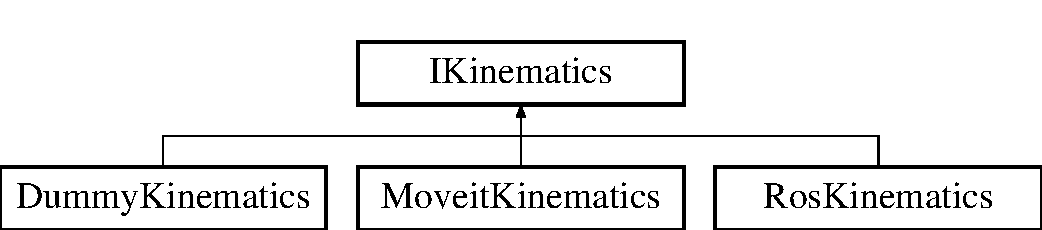
\includegraphics[height=1.996435cm]{classIKinematics}
\end{center}
\end{figure}
\subsection*{Public Member Functions}
\begin{DoxyCompactItemize}
\item 
std\-::string \& \hyperlink{classIKinematics_a1b3ec37d8072bacf767bafded072cab6}{Prefix} ()
\item 
tf\-::\-Pose \hyperlink{classIKinematics_aad69b3810156bd45c4be526ddc067358}{base\-Offset} ()
\item 
tf\-::\-Pose \hyperlink{classIKinematics_a22b46b2751763d5d2242c02de6bbd8f2}{inv\-Base\-Offset} ()
\item 
size\-\_\-t \hyperlink{classIKinematics_a95ceb0b9c129601bb54851f38e72b65a}{Num\-Joints} ()
\item 
virtual void \hyperlink{classIKinematics_a9812392000d7f06ae0353789e8e15606}{Set\-Hint} (std\-::vector$<$ double $>$ \hyperlink{classIKinematics_a7e8f1a113eafba9c64ab73a8cb279924}{hint})
\item 
virtual std\-::vector$<$ std\-::string $>$ \hyperlink{classIKinematics_a9b46e78ddaefe53f8f11221ac61b2bf5}{Joint\-Names} ()
\item 
virtual std\-::vector$<$ std\-::string $>$ \hyperlink{classIKinematics_a20a4753ef6dcd172b1a8d46a5789721c}{Link\-Names} ()
\item 
void \hyperlink{classIKinematics_ae438694ab63ef84b5f82b620d1a9ac96}{Verify\-Limits} (std\-::vector$<$ double $>$ joints)
\item 
virtual std\-::vector$<$ double $>$ \hyperlink{classIKinematics_a500626041c92cf99c7908a456f87fe0d}{Get\-Joint\-Values} ()
\begin{DoxyCompactList}\small\item\em Get\-Joint\-Values returns latest reading of end effector. \end{DoxyCompactList}\item 
virtual void \hyperlink{classIKinematics_a1292421c1061dc321016c7039692e189}{Set\-Joint\-Values} (std\-::vector$<$ double $>$ joint\-\_\-values)
\begin{DoxyCompactList}\small\item\em Set\-Joint\-Values sets the latest joint values of the robot. \end{DoxyCompactList}\item 
virtual \hyperlink{namespaceRCS_aa07e45d8a50e30064283d2b38087f999}{R\-C\-S\-::\-Pose} \hyperlink{classIKinematics_abf765053ac39fac5b94ef99e80b17f1b}{F\-K} (std\-::vector$<$ double $>$ jv)=0
\begin{DoxyCompactList}\small\item\em F\-K performs the forward kinematics using the joint values of the robot provided. \end{DoxyCompactList}\item 
virtual std\-::vector$<$ double $>$ \hyperlink{classIKinematics_ad0715c776a7eb325d2543bc34fa8114f}{I\-K} (\hyperlink{namespaceRCS_aa07e45d8a50e30064283d2b38087f999}{R\-C\-S\-::\-Pose} \&pose, std\-::vector$<$ double $>$ oldjoints)=0
\begin{DoxyCompactList}\small\item\em I\-K performs the inverse kinematics using the Cartesian pose provided. \end{DoxyCompactList}\item 
virtual std\-::vector$<$ double $>$ \hyperlink{classIKinematics_a2b5554a09667fa0b985f3954306841ea}{I\-K} (\hyperlink{namespaceRCS_aa07e45d8a50e30064283d2b38087f999}{R\-C\-S\-::\-Pose} \&pose, std\-::vector$<$ double $>$ minrange, std\-::vector$<$ double $>$ maxrange)
\begin{DoxyCompactList}\small\item\em I\-K performs the inverse kinematics using the Cartesian pose provided. \end{DoxyCompactList}\item 
virtual size\-\_\-t \hyperlink{classIKinematics_aeb53bb4b2a1e70a79d5d724e5eb82c10}{All\-Pose\-To\-Joints} (\hyperlink{namespaceRCS_aa07e45d8a50e30064283d2b38087f999}{R\-C\-S\-::\-Pose} \&pose, std\-::vector$<$ std\-::vector$<$ double $>$ $>$ \&newjoints)=0
\begin{DoxyCompactList}\small\item\em All\-Pose\-To\-Joints solves the inverse kinematics to find all solutions using the Cartesian pose provided. \end{DoxyCompactList}\item 
virtual std\-::vector$<$ double $>$ \hyperlink{classIKinematics_ab74b70ed6ecc53adfc36505b8dd1fef4}{Nearest\-Joints} (std\-::vector$<$ double $>$ oldjoints, std\-::vector$<$ std\-::vector$<$ double $>$ $>$ \&newjoints)=0
\begin{DoxyCompactList}\small\item\em Nearest\-Joints finds the joint set that is closest to the old joints. \end{DoxyCompactList}\item 
virtual void \hyperlink{classIKinematics_a87e475cccc5834a5ed6dc846af6ee6ed}{Init} (std\-::string groupname, std\-::string tiplinkname, std\-::string rootlinkname)
\begin{DoxyCompactList}\small\item\em Init is necessary for R\-O\-S to initialize it kinematics using robot model . \end{DoxyCompactList}\item 
virtual bool \hyperlink{classIKinematics_aac7d4f55bbd9228af0a7b733f857fcab}{Is\-Singular} (\hyperlink{namespaceRCS_aa07e45d8a50e30064283d2b38087f999}{R\-C\-S\-::\-Pose} \&pose, double threshold)
\begin{DoxyCompactList}\small\item\em Returns true if the determinant of the jacobian is near zero. . \end{DoxyCompactList}\item 
virtual void \hyperlink{classIKinematics_aa5c1c9225650b5225f3aa80e06ef1587}{Init} (ros\-::\-Node\-Handle \&nh)
\begin{DoxyCompactList}\small\item\em Initialize kinematics using robot\-\_\-description to fill parameters . \end{DoxyCompactList}\item 
virtual \hyperlink{RCS_8h_aa4adb93a26caa4dacba9c9614e283245}{Joint\-State} \hyperlink{classIKinematics_a69969236af3de600973b57d52444c4d7}{Update\-Joint\-State} (std\-::vector$<$ uint64\-\_\-t $>$ jointnums, \hyperlink{RCS_8h_aa4adb93a26caa4dacba9c9614e283245}{Joint\-State} oldjoints, \hyperlink{RCS_8h_aa4adb93a26caa4dacba9c9614e283245}{Joint\-State} njoints)
\item 
virtual std\-::vector$<$ double $>$ \hyperlink{classIKinematics_ab792f1f7ee1f2a34cb33eae02f1a91f9}{Find\-Bounded\-Solution} (std\-::vector$<$ std\-::vector$<$ double $>$$>$ \&solutions, std\-::vector$<$ double $>$ \&min, std\-::vector$<$ double $>$ \&max)
\item 
virtual std\-::vector$<$ double $>$ \hyperlink{classIKinematics_a5d2d196c29041544fd604409200a1437}{Find\-Bounded\-Solution} (std\-::vector$<$ std\-::vector$<$ double $>$$>$ \&solutions, boost\-::shared\-\_\-ptr$<$ \hyperlink{classIArmConfiguration}{I\-Arm\-Configuration} $>$ config)
\end{DoxyCompactItemize}
\subsection*{Public Attributes}
\begin{DoxyCompactItemize}
\item 
boost\-::shared\-\_\-ptr$<$\-::\hyperlink{classKinematics}{Kinematics} $>$ \hyperlink{classIKinematics_a4d9c2ff5cd606746f9f762d2c8e2d7c2}{armkin}
\end{DoxyCompactItemize}
\subsection*{Protected Attributes}
\begin{DoxyCompactItemize}
\item 
std\-::vector$<$ std\-::string $>$ \hyperlink{classIKinematics_abe955106c03418e9280763a85275ce0f}{joint\-\_\-names}
\item 
std\-::vector$<$ std\-::string $>$ \hyperlink{classIKinematics_a08df4ded5de908518e37687ccffe833c}{link\-\_\-names}
\item 
std\-::vector$<$ double $>$ \hyperlink{classIKinematics_a93debe94f7533c89c9c5de92159ac0c7}{jointvalues}
\item 
std\-::vector$<$ double $>$ \hyperlink{classIKinematics_ab061c2931468c4717f7cff67b697d364}{joint\-\_\-min}
\item 
std\-::vector$<$ double $>$ \hyperlink{classIKinematics_a4422f638d9b33ef9ccc9837ac8c1d76d}{joint\-\_\-max}
\item 
std\-::vector$<$ double $>$ \hyperlink{classIKinematics_a7e8f1a113eafba9c64ab73a8cb279924}{hint}
\item 
size\-\_\-t \hyperlink{classIKinematics_aabe89b2b82b30cdbb97545079d743222}{num\-\_\-joints}
\item 
std\-::string \hyperlink{classIKinematics_a77e5652ef78f21df82a7778e814ad234}{\-\_\-groupname}
\item 
std\-::string \hyperlink{classIKinematics_a88100365db2c65ae406c6727861261f3}{\-\_\-tiplinkname}
\item 
std\-::string \hyperlink{classIKinematics_a8e6174990e9a54967482dc0a99311976}{\-\_\-rootlinkname}
\item 
std\-::string \hyperlink{classIKinematics_a62baaf78436911eca42896cad4b5c911}{prefix}
\item 
tf\-::\-Pose \hyperlink{classIKinematics_aa599f7938cbf1c9b422a6d4d50e8e1a9}{baseoffset}
\end{DoxyCompactItemize}


\subsection{Detailed Description}
The \hyperlink{classIKinematics}{I\-Kinematics} provides is an abstract class with pure virtual functions that are overriden by actual kinematic implementations. 

\subsection{Member Function Documentation}
\hypertarget{classIKinematics_aeb53bb4b2a1e70a79d5d724e5eb82c10}{\index{I\-Kinematics@{I\-Kinematics}!All\-Pose\-To\-Joints@{All\-Pose\-To\-Joints}}
\index{All\-Pose\-To\-Joints@{All\-Pose\-To\-Joints}!IKinematics@{I\-Kinematics}}
\subsubsection[{All\-Pose\-To\-Joints}]{\setlength{\rightskip}{0pt plus 5cm}virtual size\-\_\-t I\-Kinematics\-::\-All\-Pose\-To\-Joints (
\begin{DoxyParamCaption}
\item[{{\bf R\-C\-S\-::\-Pose} \&}]{pose, }
\item[{std\-::vector$<$ std\-::vector$<$ double $>$ $>$ \&}]{newjoints}
\end{DoxyParamCaption}
)\hspace{0.3cm}{\ttfamily [pure virtual]}}}\label{classIKinematics_aeb53bb4b2a1e70a79d5d724e5eb82c10}


All\-Pose\-To\-Joints solves the inverse kinematics to find all solutions using the Cartesian pose provided. 


\begin{DoxyParams}{Parameters}
{\em Cartesian} & robot pose of end effector. \\
\hline
{\em vector} & of double vectos to hold all the I\-K joint solutions. \\
\hline
\end{DoxyParams}
\begin{DoxyReturn}{Returns}
number of solutions found. 
\end{DoxyReturn}


Implemented in \hyperlink{classFanucLrMate200idKinematics_a9273cba3818f4ce905f45643d8056eea}{Fanuc\-Lr\-Mate200id\-Kinematics}, and \hyperlink{classArmKinematics_a18053e73102f70dfe7260eafe48b3548}{Arm\-Kinematics}.

\hypertarget{classIKinematics_aad69b3810156bd45c4be526ddc067358}{\index{I\-Kinematics@{I\-Kinematics}!base\-Offset@{base\-Offset}}
\index{base\-Offset@{base\-Offset}!IKinematics@{I\-Kinematics}}
\subsubsection[{base\-Offset}]{\setlength{\rightskip}{0pt plus 5cm}tf\-::\-Pose I\-Kinematics\-::base\-Offset (
\begin{DoxyParamCaption}
{}
\end{DoxyParamCaption}
)\hspace{0.3cm}{\ttfamily [inline]}}}\label{classIKinematics_aad69b3810156bd45c4be526ddc067358}
\hypertarget{classIKinematics_ab792f1f7ee1f2a34cb33eae02f1a91f9}{\index{I\-Kinematics@{I\-Kinematics}!Find\-Bounded\-Solution@{Find\-Bounded\-Solution}}
\index{Find\-Bounded\-Solution@{Find\-Bounded\-Solution}!IKinematics@{I\-Kinematics}}
\subsubsection[{Find\-Bounded\-Solution}]{\setlength{\rightskip}{0pt plus 5cm}virtual std\-::vector$<$double$>$ I\-Kinematics\-::\-Find\-Bounded\-Solution (
\begin{DoxyParamCaption}
\item[{std\-::vector$<$ std\-::vector$<$ double $>$$>$ \&}]{solutions, }
\item[{std\-::vector$<$ double $>$ \&}]{min, }
\item[{std\-::vector$<$ double $>$ \&}]{max}
\end{DoxyParamCaption}
)\hspace{0.3cm}{\ttfamily [inline]}, {\ttfamily [virtual]}}}\label{classIKinematics_ab792f1f7ee1f2a34cb33eae02f1a91f9}


Reimplemented in \hyperlink{classFastKinematics_a811d12eb6c664d72d4ae5a685d219185}{Fast\-Kinematics}.

\hypertarget{classIKinematics_a5d2d196c29041544fd604409200a1437}{\index{I\-Kinematics@{I\-Kinematics}!Find\-Bounded\-Solution@{Find\-Bounded\-Solution}}
\index{Find\-Bounded\-Solution@{Find\-Bounded\-Solution}!IKinematics@{I\-Kinematics}}
\subsubsection[{Find\-Bounded\-Solution}]{\setlength{\rightskip}{0pt plus 5cm}virtual std\-::vector$<$double$>$ I\-Kinematics\-::\-Find\-Bounded\-Solution (
\begin{DoxyParamCaption}
\item[{std\-::vector$<$ std\-::vector$<$ double $>$$>$ \&}]{solutions, }
\item[{boost\-::shared\-\_\-ptr$<$ {\bf I\-Arm\-Configuration} $>$}]{config}
\end{DoxyParamCaption}
)\hspace{0.3cm}{\ttfamily [inline]}, {\ttfamily [virtual]}}}\label{classIKinematics_a5d2d196c29041544fd604409200a1437}
\hypertarget{classIKinematics_abf765053ac39fac5b94ef99e80b17f1b}{\index{I\-Kinematics@{I\-Kinematics}!F\-K@{F\-K}}
\index{F\-K@{F\-K}!IKinematics@{I\-Kinematics}}
\subsubsection[{F\-K}]{\setlength{\rightskip}{0pt plus 5cm}virtual {\bf R\-C\-S\-::\-Pose} I\-Kinematics\-::\-F\-K (
\begin{DoxyParamCaption}
\item[{std\-::vector$<$ double $>$}]{jv}
\end{DoxyParamCaption}
)\hspace{0.3cm}{\ttfamily [pure virtual]}}}\label{classIKinematics_abf765053ac39fac5b94ef99e80b17f1b}


F\-K performs the forward kinematics using the joint values of the robot provided. 


\begin{DoxyParams}{Parameters}
{\em vector} & of all robot joint values in doubles. \\
\hline
\end{DoxyParams}
\begin{DoxyReturn}{Returns}
corresponding Cartesian robot pose of end effector. 
\end{DoxyReturn}


Implemented in \hyperlink{classFanucLrMate200idKinematics_a42b44b203b26d356dd9cc7769658138e}{Fanuc\-Lr\-Mate200id\-Kinematics}, \hyperlink{classFastKinematics_ad60c8729768b34e653c484a476d471a1}{Fast\-Kinematics}, and \hyperlink{classArmKinematics_a1773ef10fcdd9bfb7b5d806c42bcbfb1}{Arm\-Kinematics}.

\hypertarget{classIKinematics_a500626041c92cf99c7908a456f87fe0d}{\index{I\-Kinematics@{I\-Kinematics}!Get\-Joint\-Values@{Get\-Joint\-Values}}
\index{Get\-Joint\-Values@{Get\-Joint\-Values}!IKinematics@{I\-Kinematics}}
\subsubsection[{Get\-Joint\-Values}]{\setlength{\rightskip}{0pt plus 5cm}virtual std\-::vector$<$double$>$ I\-Kinematics\-::\-Get\-Joint\-Values (
\begin{DoxyParamCaption}
{}
\end{DoxyParamCaption}
)\hspace{0.3cm}{\ttfamily [inline]}, {\ttfamily [virtual]}}}\label{classIKinematics_a500626041c92cf99c7908a456f87fe0d}


Get\-Joint\-Values returns latest reading of end effector. 

\begin{DoxyReturn}{Returns}
vector of joint values in doubles. 
\end{DoxyReturn}
\hypertarget{classIKinematics_ad0715c776a7eb325d2543bc34fa8114f}{\index{I\-Kinematics@{I\-Kinematics}!I\-K@{I\-K}}
\index{I\-K@{I\-K}!IKinematics@{I\-Kinematics}}
\subsubsection[{I\-K}]{\setlength{\rightskip}{0pt plus 5cm}virtual std\-::vector$<$double$>$ I\-Kinematics\-::\-I\-K (
\begin{DoxyParamCaption}
\item[{{\bf R\-C\-S\-::\-Pose} \&}]{pose, }
\item[{std\-::vector$<$ double $>$}]{oldjoints}
\end{DoxyParamCaption}
)\hspace{0.3cm}{\ttfamily [pure virtual]}}}\label{classIKinematics_ad0715c776a7eb325d2543bc34fa8114f}


I\-K performs the inverse kinematics using the Cartesian pose provided. 


\begin{DoxyParams}{Parameters}
{\em Cartesian} & robot pose of end effector. \\
\hline
{\em optional} & seed joint values to use as best guess for I\-K joint values. \\
\hline
\end{DoxyParams}
\begin{DoxyReturn}{Returns}
vector of all robot joint values in doubles. 
\end{DoxyReturn}


Implemented in \hyperlink{classFanucLrMate200idKinematics_a54a3ef5b0e8db49e1ee3362ba2642df6}{Fanuc\-Lr\-Mate200id\-Kinematics}, \hyperlink{classFastKinematics_ad71d66aa03ef1c2d24a190346aa304a1}{Fast\-Kinematics}, and \hyperlink{classArmKinematics_a28e91de4fcb7ae0e8d4ce7d83bef2165}{Arm\-Kinematics}.

\hypertarget{classIKinematics_a2b5554a09667fa0b985f3954306841ea}{\index{I\-Kinematics@{I\-Kinematics}!I\-K@{I\-K}}
\index{I\-K@{I\-K}!IKinematics@{I\-Kinematics}}
\subsubsection[{I\-K}]{\setlength{\rightskip}{0pt plus 5cm}virtual std\-::vector$<$double$>$ I\-Kinematics\-::\-I\-K (
\begin{DoxyParamCaption}
\item[{{\bf R\-C\-S\-::\-Pose} \&}]{pose, }
\item[{std\-::vector$<$ double $>$}]{minrange, }
\item[{std\-::vector$<$ double $>$}]{maxrange}
\end{DoxyParamCaption}
)\hspace{0.3cm}{\ttfamily [inline]}, {\ttfamily [virtual]}}}\label{classIKinematics_a2b5554a09667fa0b985f3954306841ea}


I\-K performs the inverse kinematics using the Cartesian pose provided. 


\begin{DoxyParams}{Parameters}
{\em Cartesian} & robot pose of end effector. \\
\hline
{\em optional} & seed joint values to use as best guess for I\-K joint values. \\
\hline
\end{DoxyParams}
\begin{DoxyReturn}{Returns}
vector of all robot joint values in doubles. 
\end{DoxyReturn}


Reimplemented in \hyperlink{classFastKinematics_a9f9b4b4f95039605a243a85adacd207f}{Fast\-Kinematics}.

\hypertarget{classIKinematics_a87e475cccc5834a5ed6dc846af6ee6ed}{\index{I\-Kinematics@{I\-Kinematics}!Init@{Init}}
\index{Init@{Init}!IKinematics@{I\-Kinematics}}
\subsubsection[{Init}]{\setlength{\rightskip}{0pt plus 5cm}virtual void I\-Kinematics\-::\-Init (
\begin{DoxyParamCaption}
\item[{std\-::string}]{groupname, }
\item[{std\-::string}]{tiplinkname, }
\item[{std\-::string}]{rootlinkname}
\end{DoxyParamCaption}
)\hspace{0.3cm}{\ttfamily [inline]}, {\ttfamily [virtual]}}}\label{classIKinematics_a87e475cccc5834a5ed6dc846af6ee6ed}


Init is necessary for R\-O\-S to initialize it kinematics using robot model . 


\begin{DoxyParams}{Parameters}
{\em groupname} & name of chained joints in robot model. \\
\hline
{\em eelinkname} & name of end effector joint in robot model. \\
\hline
\end{DoxyParams}
\hypertarget{classIKinematics_aa5c1c9225650b5225f3aa80e06ef1587}{\index{I\-Kinematics@{I\-Kinematics}!Init@{Init}}
\index{Init@{Init}!IKinematics@{I\-Kinematics}}
\subsubsection[{Init}]{\setlength{\rightskip}{0pt plus 5cm}virtual void I\-Kinematics\-::\-Init (
\begin{DoxyParamCaption}
\item[{ros\-::\-Node\-Handle \&}]{nh}
\end{DoxyParamCaption}
)\hspace{0.3cm}{\ttfamily [inline]}, {\ttfamily [virtual]}}}\label{classIKinematics_aa5c1c9225650b5225f3aa80e06ef1587}


Initialize kinematics using robot\-\_\-description to fill parameters . 


\begin{DoxyParams}{Parameters}
{\em nh} & ros node handle of node. \\
\hline
\end{DoxyParams}


Reimplemented in \hyperlink{classFanucLrMate200idKinematics_a40dceae1773781d021c86aea16e40da8}{Fanuc\-Lr\-Mate200id\-Kinematics}, \hyperlink{classFastKinematics_af2de2a0ac3576faffa13dd5357561f78}{Fast\-Kinematics}, and \hyperlink{classArmKinematics_accebfc031ce46ca59279cca01c152149}{Arm\-Kinematics}.

\hypertarget{classIKinematics_a22b46b2751763d5d2242c02de6bbd8f2}{\index{I\-Kinematics@{I\-Kinematics}!inv\-Base\-Offset@{inv\-Base\-Offset}}
\index{inv\-Base\-Offset@{inv\-Base\-Offset}!IKinematics@{I\-Kinematics}}
\subsubsection[{inv\-Base\-Offset}]{\setlength{\rightskip}{0pt plus 5cm}tf\-::\-Pose I\-Kinematics\-::inv\-Base\-Offset (
\begin{DoxyParamCaption}
{}
\end{DoxyParamCaption}
)\hspace{0.3cm}{\ttfamily [inline]}}}\label{classIKinematics_a22b46b2751763d5d2242c02de6bbd8f2}
\hypertarget{classIKinematics_aac7d4f55bbd9228af0a7b733f857fcab}{\index{I\-Kinematics@{I\-Kinematics}!Is\-Singular@{Is\-Singular}}
\index{Is\-Singular@{Is\-Singular}!IKinematics@{I\-Kinematics}}
\subsubsection[{Is\-Singular}]{\setlength{\rightskip}{0pt plus 5cm}virtual bool I\-Kinematics\-::\-Is\-Singular (
\begin{DoxyParamCaption}
\item[{{\bf R\-C\-S\-::\-Pose} \&}]{pose, }
\item[{double}]{threshold}
\end{DoxyParamCaption}
)\hspace{0.3cm}{\ttfamily [inline]}, {\ttfamily [virtual]}}}\label{classIKinematics_aac7d4f55bbd9228af0a7b733f857fcab}


Returns true if the determinant of the jacobian is near zero. . 


\begin{DoxyParams}{Parameters}
{\em groupname} & name of chained joints in robot model. \\
\hline
{\em eelinkname} & name of end effector joint in robot model. \\
\hline
\end{DoxyParams}


Reimplemented in \hyperlink{classFastKinematics_a00652f1e5f1f7bfb9b450576beb7b71f}{Fast\-Kinematics}, and \hyperlink{classArmKinematics_af0ef95a582ede450b2bce813340a88cb}{Arm\-Kinematics}.

\hypertarget{classIKinematics_a9b46e78ddaefe53f8f11221ac61b2bf5}{\index{I\-Kinematics@{I\-Kinematics}!Joint\-Names@{Joint\-Names}}
\index{Joint\-Names@{Joint\-Names}!IKinematics@{I\-Kinematics}}
\subsubsection[{Joint\-Names}]{\setlength{\rightskip}{0pt plus 5cm}virtual std\-::vector$<$std\-::string$>$ I\-Kinematics\-::\-Joint\-Names (
\begin{DoxyParamCaption}
{}
\end{DoxyParamCaption}
)\hspace{0.3cm}{\ttfamily [inline]}, {\ttfamily [virtual]}}}\label{classIKinematics_a9b46e78ddaefe53f8f11221ac61b2bf5}
\hypertarget{classIKinematics_a20a4753ef6dcd172b1a8d46a5789721c}{\index{I\-Kinematics@{I\-Kinematics}!Link\-Names@{Link\-Names}}
\index{Link\-Names@{Link\-Names}!IKinematics@{I\-Kinematics}}
\subsubsection[{Link\-Names}]{\setlength{\rightskip}{0pt plus 5cm}virtual std\-::vector$<$std\-::string$>$ I\-Kinematics\-::\-Link\-Names (
\begin{DoxyParamCaption}
{}
\end{DoxyParamCaption}
)\hspace{0.3cm}{\ttfamily [inline]}, {\ttfamily [virtual]}}}\label{classIKinematics_a20a4753ef6dcd172b1a8d46a5789721c}
\hypertarget{classIKinematics_ab74b70ed6ecc53adfc36505b8dd1fef4}{\index{I\-Kinematics@{I\-Kinematics}!Nearest\-Joints@{Nearest\-Joints}}
\index{Nearest\-Joints@{Nearest\-Joints}!IKinematics@{I\-Kinematics}}
\subsubsection[{Nearest\-Joints}]{\setlength{\rightskip}{0pt plus 5cm}virtual std\-::vector$<$double$>$ I\-Kinematics\-::\-Nearest\-Joints (
\begin{DoxyParamCaption}
\item[{std\-::vector$<$ double $>$}]{oldjoints, }
\item[{std\-::vector$<$ std\-::vector$<$ double $>$ $>$ \&}]{newjoints}
\end{DoxyParamCaption}
)\hspace{0.3cm}{\ttfamily [pure virtual]}}}\label{classIKinematics_ab74b70ed6ecc53adfc36505b8dd1fef4}


Nearest\-Joints finds the joint set that is closest to the old joints. 


\begin{DoxyParams}{Parameters}
{\em old} & seed joint values to use as best guess for I\-K joint values. \\
\hline
{\em vector} & of double vectos that holds all the I\-K joint solutions. \\
\hline
\end{DoxyParams}
\begin{DoxyReturn}{Returns}
vector of doubles with closest set to seed joints. 
\end{DoxyReturn}


Implemented in \hyperlink{classFanucLrMate200idKinematics_ad7ec485c3eb09775d09512b0e15d3f84}{Fanuc\-Lr\-Mate200id\-Kinematics}, and \hyperlink{classArmKinematics_a7836b4724f8036ca171c21b9877b7a7e}{Arm\-Kinematics}.

\hypertarget{classIKinematics_a95ceb0b9c129601bb54851f38e72b65a}{\index{I\-Kinematics@{I\-Kinematics}!Num\-Joints@{Num\-Joints}}
\index{Num\-Joints@{Num\-Joints}!IKinematics@{I\-Kinematics}}
\subsubsection[{Num\-Joints}]{\setlength{\rightskip}{0pt plus 5cm}size\-\_\-t I\-Kinematics\-::\-Num\-Joints (
\begin{DoxyParamCaption}
{}
\end{DoxyParamCaption}
)\hspace{0.3cm}{\ttfamily [inline]}}}\label{classIKinematics_a95ceb0b9c129601bb54851f38e72b65a}
\hypertarget{classIKinematics_a1b3ec37d8072bacf767bafded072cab6}{\index{I\-Kinematics@{I\-Kinematics}!Prefix@{Prefix}}
\index{Prefix@{Prefix}!IKinematics@{I\-Kinematics}}
\subsubsection[{Prefix}]{\setlength{\rightskip}{0pt plus 5cm}std\-::string\& I\-Kinematics\-::\-Prefix (
\begin{DoxyParamCaption}
{}
\end{DoxyParamCaption}
)\hspace{0.3cm}{\ttfamily [inline]}}}\label{classIKinematics_a1b3ec37d8072bacf767bafded072cab6}
\hypertarget{classIKinematics_a9812392000d7f06ae0353789e8e15606}{\index{I\-Kinematics@{I\-Kinematics}!Set\-Hint@{Set\-Hint}}
\index{Set\-Hint@{Set\-Hint}!IKinematics@{I\-Kinematics}}
\subsubsection[{Set\-Hint}]{\setlength{\rightskip}{0pt plus 5cm}virtual void I\-Kinematics\-::\-Set\-Hint (
\begin{DoxyParamCaption}
\item[{std\-::vector$<$ double $>$}]{hint}
\end{DoxyParamCaption}
)\hspace{0.3cm}{\ttfamily [inline]}, {\ttfamily [virtual]}}}\label{classIKinematics_a9812392000d7f06ae0353789e8e15606}
\hypertarget{classIKinematics_a1292421c1061dc321016c7039692e189}{\index{I\-Kinematics@{I\-Kinematics}!Set\-Joint\-Values@{Set\-Joint\-Values}}
\index{Set\-Joint\-Values@{Set\-Joint\-Values}!IKinematics@{I\-Kinematics}}
\subsubsection[{Set\-Joint\-Values}]{\setlength{\rightskip}{0pt plus 5cm}virtual void I\-Kinematics\-::\-Set\-Joint\-Values (
\begin{DoxyParamCaption}
\item[{std\-::vector$<$ double $>$}]{joint\-\_\-values}
\end{DoxyParamCaption}
)\hspace{0.3cm}{\ttfamily [inline]}, {\ttfamily [virtual]}}}\label{classIKinematics_a1292421c1061dc321016c7039692e189}


Set\-Joint\-Values sets the latest joint values of the robot. 


\begin{DoxyParams}{Parameters}
{\em vector} & of all robot joint values in doubles. \\
\hline
\end{DoxyParams}
\hypertarget{classIKinematics_a69969236af3de600973b57d52444c4d7}{\index{I\-Kinematics@{I\-Kinematics}!Update\-Joint\-State@{Update\-Joint\-State}}
\index{Update\-Joint\-State@{Update\-Joint\-State}!IKinematics@{I\-Kinematics}}
\subsubsection[{Update\-Joint\-State}]{\setlength{\rightskip}{0pt plus 5cm}virtual {\bf Joint\-State} I\-Kinematics\-::\-Update\-Joint\-State (
\begin{DoxyParamCaption}
\item[{std\-::vector$<$ uint64\-\_\-t $>$}]{jointnums, }
\item[{{\bf Joint\-State}}]{oldjoints, }
\item[{{\bf Joint\-State}}]{njoints}
\end{DoxyParamCaption}
)\hspace{0.3cm}{\ttfamily [inline]}, {\ttfamily [virtual]}}}\label{classIKinematics_a69969236af3de600973b57d52444c4d7}
\hypertarget{classIKinematics_ae438694ab63ef84b5f82b620d1a9ac96}{\index{I\-Kinematics@{I\-Kinematics}!Verify\-Limits@{Verify\-Limits}}
\index{Verify\-Limits@{Verify\-Limits}!IKinematics@{I\-Kinematics}}
\subsubsection[{Verify\-Limits}]{\setlength{\rightskip}{0pt plus 5cm}void I\-Kinematics\-::\-Verify\-Limits (
\begin{DoxyParamCaption}
\item[{std\-::vector$<$ double $>$}]{joints}
\end{DoxyParamCaption}
)\hspace{0.3cm}{\ttfamily [inline]}}}\label{classIKinematics_ae438694ab63ef84b5f82b620d1a9ac96}


\subsection{Member Data Documentation}
\hypertarget{classIKinematics_a77e5652ef78f21df82a7778e814ad234}{\index{I\-Kinematics@{I\-Kinematics}!\-\_\-groupname@{\-\_\-groupname}}
\index{\-\_\-groupname@{\-\_\-groupname}!IKinematics@{I\-Kinematics}}
\subsubsection[{\-\_\-groupname}]{\setlength{\rightskip}{0pt plus 5cm}std\-::string I\-Kinematics\-::\-\_\-groupname\hspace{0.3cm}{\ttfamily [protected]}}}\label{classIKinematics_a77e5652ef78f21df82a7778e814ad234}
\hypertarget{classIKinematics_a8e6174990e9a54967482dc0a99311976}{\index{I\-Kinematics@{I\-Kinematics}!\-\_\-rootlinkname@{\-\_\-rootlinkname}}
\index{\-\_\-rootlinkname@{\-\_\-rootlinkname}!IKinematics@{I\-Kinematics}}
\subsubsection[{\-\_\-rootlinkname}]{\setlength{\rightskip}{0pt plus 5cm}std\-::string I\-Kinematics\-::\-\_\-rootlinkname\hspace{0.3cm}{\ttfamily [protected]}}}\label{classIKinematics_a8e6174990e9a54967482dc0a99311976}
\hypertarget{classIKinematics_a88100365db2c65ae406c6727861261f3}{\index{I\-Kinematics@{I\-Kinematics}!\-\_\-tiplinkname@{\-\_\-tiplinkname}}
\index{\-\_\-tiplinkname@{\-\_\-tiplinkname}!IKinematics@{I\-Kinematics}}
\subsubsection[{\-\_\-tiplinkname}]{\setlength{\rightskip}{0pt plus 5cm}std\-::string I\-Kinematics\-::\-\_\-tiplinkname\hspace{0.3cm}{\ttfamily [protected]}}}\label{classIKinematics_a88100365db2c65ae406c6727861261f3}
\hypertarget{classIKinematics_a4d9c2ff5cd606746f9f762d2c8e2d7c2}{\index{I\-Kinematics@{I\-Kinematics}!armkin@{armkin}}
\index{armkin@{armkin}!IKinematics@{I\-Kinematics}}
\subsubsection[{armkin}]{\setlength{\rightskip}{0pt plus 5cm}boost\-::shared\-\_\-ptr$<$\-::{\bf Kinematics}$>$ I\-Kinematics\-::armkin}}\label{classIKinematics_a4d9c2ff5cd606746f9f762d2c8e2d7c2}
\hypertarget{classIKinematics_aa599f7938cbf1c9b422a6d4d50e8e1a9}{\index{I\-Kinematics@{I\-Kinematics}!baseoffset@{baseoffset}}
\index{baseoffset@{baseoffset}!IKinematics@{I\-Kinematics}}
\subsubsection[{baseoffset}]{\setlength{\rightskip}{0pt plus 5cm}tf\-::\-Pose I\-Kinematics\-::baseoffset\hspace{0.3cm}{\ttfamily [protected]}}}\label{classIKinematics_aa599f7938cbf1c9b422a6d4d50e8e1a9}
\hypertarget{classIKinematics_a7e8f1a113eafba9c64ab73a8cb279924}{\index{I\-Kinematics@{I\-Kinematics}!hint@{hint}}
\index{hint@{hint}!IKinematics@{I\-Kinematics}}
\subsubsection[{hint}]{\setlength{\rightskip}{0pt plus 5cm}std\-::vector$<$ double$>$ I\-Kinematics\-::hint\hspace{0.3cm}{\ttfamily [protected]}}}\label{classIKinematics_a7e8f1a113eafba9c64ab73a8cb279924}
\hypertarget{classIKinematics_a4422f638d9b33ef9ccc9837ac8c1d76d}{\index{I\-Kinematics@{I\-Kinematics}!joint\-\_\-max@{joint\-\_\-max}}
\index{joint\-\_\-max@{joint\-\_\-max}!IKinematics@{I\-Kinematics}}
\subsubsection[{joint\-\_\-max}]{\setlength{\rightskip}{0pt plus 5cm}std\-::vector$<$ double$>$ I\-Kinematics\-::joint\-\_\-max\hspace{0.3cm}{\ttfamily [protected]}}}\label{classIKinematics_a4422f638d9b33ef9ccc9837ac8c1d76d}
\hypertarget{classIKinematics_ab061c2931468c4717f7cff67b697d364}{\index{I\-Kinematics@{I\-Kinematics}!joint\-\_\-min@{joint\-\_\-min}}
\index{joint\-\_\-min@{joint\-\_\-min}!IKinematics@{I\-Kinematics}}
\subsubsection[{joint\-\_\-min}]{\setlength{\rightskip}{0pt plus 5cm}std\-::vector$<$ double$>$ I\-Kinematics\-::joint\-\_\-min\hspace{0.3cm}{\ttfamily [protected]}}}\label{classIKinematics_ab061c2931468c4717f7cff67b697d364}
\hypertarget{classIKinematics_abe955106c03418e9280763a85275ce0f}{\index{I\-Kinematics@{I\-Kinematics}!joint\-\_\-names@{joint\-\_\-names}}
\index{joint\-\_\-names@{joint\-\_\-names}!IKinematics@{I\-Kinematics}}
\subsubsection[{joint\-\_\-names}]{\setlength{\rightskip}{0pt plus 5cm}std\-::vector$<$std\-::string$>$ I\-Kinematics\-::joint\-\_\-names\hspace{0.3cm}{\ttfamily [protected]}}}\label{classIKinematics_abe955106c03418e9280763a85275ce0f}
\hypertarget{classIKinematics_a93debe94f7533c89c9c5de92159ac0c7}{\index{I\-Kinematics@{I\-Kinematics}!jointvalues@{jointvalues}}
\index{jointvalues@{jointvalues}!IKinematics@{I\-Kinematics}}
\subsubsection[{jointvalues}]{\setlength{\rightskip}{0pt plus 5cm}std\-::vector$<$ double$>$ I\-Kinematics\-::jointvalues\hspace{0.3cm}{\ttfamily [protected]}}}\label{classIKinematics_a93debe94f7533c89c9c5de92159ac0c7}
\hypertarget{classIKinematics_a08df4ded5de908518e37687ccffe833c}{\index{I\-Kinematics@{I\-Kinematics}!link\-\_\-names@{link\-\_\-names}}
\index{link\-\_\-names@{link\-\_\-names}!IKinematics@{I\-Kinematics}}
\subsubsection[{link\-\_\-names}]{\setlength{\rightskip}{0pt plus 5cm}std\-::vector$<$std\-::string$>$ I\-Kinematics\-::link\-\_\-names\hspace{0.3cm}{\ttfamily [protected]}}}\label{classIKinematics_a08df4ded5de908518e37687ccffe833c}
\hypertarget{classIKinematics_aabe89b2b82b30cdbb97545079d743222}{\index{I\-Kinematics@{I\-Kinematics}!num\-\_\-joints@{num\-\_\-joints}}
\index{num\-\_\-joints@{num\-\_\-joints}!IKinematics@{I\-Kinematics}}
\subsubsection[{num\-\_\-joints}]{\setlength{\rightskip}{0pt plus 5cm}size\-\_\-t I\-Kinematics\-::num\-\_\-joints\hspace{0.3cm}{\ttfamily [protected]}}}\label{classIKinematics_aabe89b2b82b30cdbb97545079d743222}
\hypertarget{classIKinematics_a62baaf78436911eca42896cad4b5c911}{\index{I\-Kinematics@{I\-Kinematics}!prefix@{prefix}}
\index{prefix@{prefix}!IKinematics@{I\-Kinematics}}
\subsubsection[{prefix}]{\setlength{\rightskip}{0pt plus 5cm}std\-::string I\-Kinematics\-::prefix\hspace{0.3cm}{\ttfamily [protected]}}}\label{classIKinematics_a62baaf78436911eca42896cad4b5c911}


The documentation for this class was generated from the following file\-:\begin{DoxyCompactItemize}
\item 
/usr/local/michalos/nistfanuc\-\_\-ws/src/nist\-\_\-fanuc/include/nist\-\_\-fanuc/\hyperlink{Kinematics_8h}{Kinematics.\-h}\end{DoxyCompactItemize}

\hypertarget{classikfast_1_1IkSingleDOFSolutionBase}{\section{ikfast\-:\-:Ik\-Single\-D\-O\-F\-Solution\-Base$<$ T $>$ Class Template Reference}
\label{classikfast_1_1IkSingleDOFSolutionBase}\index{ikfast\-::\-Ik\-Single\-D\-O\-F\-Solution\-Base$<$ T $>$@{ikfast\-::\-Ik\-Single\-D\-O\-F\-Solution\-Base$<$ T $>$}}
}


{\ttfamily \#include $<$ikfast.\-h$>$}

\subsection*{Public Member Functions}
\begin{DoxyCompactItemize}
\item 
\hyperlink{classikfast_1_1IkSingleDOFSolutionBase_aa3c37c6e9a4903f1303893e966260789}{Ik\-Single\-D\-O\-F\-Solution\-Base} ()
\end{DoxyCompactItemize}
\subsection*{Public Attributes}
\begin{DoxyCompactItemize}
\item 
T \hyperlink{classikfast_1_1IkSingleDOFSolutionBase_adb64a33a2ce7357684c9c89d75cacd0c}{fmul}
\item 
T \hyperlink{classikfast_1_1IkSingleDOFSolutionBase_a1d5900ae9cb2d55c396b995b976fdcef}{foffset}
\item 
signed char \hyperlink{classikfast_1_1IkSingleDOFSolutionBase_adca245b0afa4133dddbd10803053bc2a}{freeind}
\item 
unsigned char \hyperlink{classikfast_1_1IkSingleDOFSolutionBase_a3c458c4a2b06b4a2ccffc265cf34c6fe}{jointtype}
\item 
unsigned char \hyperlink{classikfast_1_1IkSingleDOFSolutionBase_a45404bf30c7b90131b7ce2b8045c6f6a}{maxsolutions}
\item 
unsigned char \hyperlink{classikfast_1_1IkSingleDOFSolutionBase_a50d8439b7f735a474f6dfe42e91de455}{indices} \mbox{[}5\mbox{]}
\end{DoxyCompactItemize}


\subsection{Constructor \& Destructor Documentation}
\hypertarget{classikfast_1_1IkSingleDOFSolutionBase_aa3c37c6e9a4903f1303893e966260789}{\index{ikfast\-::\-Ik\-Single\-D\-O\-F\-Solution\-Base@{ikfast\-::\-Ik\-Single\-D\-O\-F\-Solution\-Base}!Ik\-Single\-D\-O\-F\-Solution\-Base@{Ik\-Single\-D\-O\-F\-Solution\-Base}}
\index{Ik\-Single\-D\-O\-F\-Solution\-Base@{Ik\-Single\-D\-O\-F\-Solution\-Base}!ikfast::IkSingleDOFSolutionBase@{ikfast\-::\-Ik\-Single\-D\-O\-F\-Solution\-Base}}
\subsubsection[{Ik\-Single\-D\-O\-F\-Solution\-Base}]{\setlength{\rightskip}{0pt plus 5cm}template$<$typename T $>$ {\bf ikfast\-::\-Ik\-Single\-D\-O\-F\-Solution\-Base}$<$ T $>$\-::{\bf Ik\-Single\-D\-O\-F\-Solution\-Base} (
\begin{DoxyParamCaption}
{}
\end{DoxyParamCaption}
)\hspace{0.3cm}{\ttfamily [inline]}}}\label{classikfast_1_1IkSingleDOFSolutionBase_aa3c37c6e9a4903f1303893e966260789}


\subsection{Member Data Documentation}
\hypertarget{classikfast_1_1IkSingleDOFSolutionBase_adb64a33a2ce7357684c9c89d75cacd0c}{\index{ikfast\-::\-Ik\-Single\-D\-O\-F\-Solution\-Base@{ikfast\-::\-Ik\-Single\-D\-O\-F\-Solution\-Base}!fmul@{fmul}}
\index{fmul@{fmul}!ikfast::IkSingleDOFSolutionBase@{ikfast\-::\-Ik\-Single\-D\-O\-F\-Solution\-Base}}
\subsubsection[{fmul}]{\setlength{\rightskip}{0pt plus 5cm}template$<$typename T $>$ T {\bf ikfast\-::\-Ik\-Single\-D\-O\-F\-Solution\-Base}$<$ T $>$\-::fmul}}\label{classikfast_1_1IkSingleDOFSolutionBase_adb64a33a2ce7357684c9c89d75cacd0c}
\hypertarget{classikfast_1_1IkSingleDOFSolutionBase_a1d5900ae9cb2d55c396b995b976fdcef}{\index{ikfast\-::\-Ik\-Single\-D\-O\-F\-Solution\-Base@{ikfast\-::\-Ik\-Single\-D\-O\-F\-Solution\-Base}!foffset@{foffset}}
\index{foffset@{foffset}!ikfast::IkSingleDOFSolutionBase@{ikfast\-::\-Ik\-Single\-D\-O\-F\-Solution\-Base}}
\subsubsection[{foffset}]{\setlength{\rightskip}{0pt plus 5cm}template$<$typename T $>$ T {\bf ikfast\-::\-Ik\-Single\-D\-O\-F\-Solution\-Base}$<$ T $>$\-::foffset}}\label{classikfast_1_1IkSingleDOFSolutionBase_a1d5900ae9cb2d55c396b995b976fdcef}
\hypertarget{classikfast_1_1IkSingleDOFSolutionBase_adca245b0afa4133dddbd10803053bc2a}{\index{ikfast\-::\-Ik\-Single\-D\-O\-F\-Solution\-Base@{ikfast\-::\-Ik\-Single\-D\-O\-F\-Solution\-Base}!freeind@{freeind}}
\index{freeind@{freeind}!ikfast::IkSingleDOFSolutionBase@{ikfast\-::\-Ik\-Single\-D\-O\-F\-Solution\-Base}}
\subsubsection[{freeind}]{\setlength{\rightskip}{0pt plus 5cm}template$<$typename T $>$ signed char {\bf ikfast\-::\-Ik\-Single\-D\-O\-F\-Solution\-Base}$<$ T $>$\-::freeind}}\label{classikfast_1_1IkSingleDOFSolutionBase_adca245b0afa4133dddbd10803053bc2a}
\hypertarget{classikfast_1_1IkSingleDOFSolutionBase_a50d8439b7f735a474f6dfe42e91de455}{\index{ikfast\-::\-Ik\-Single\-D\-O\-F\-Solution\-Base@{ikfast\-::\-Ik\-Single\-D\-O\-F\-Solution\-Base}!indices@{indices}}
\index{indices@{indices}!ikfast::IkSingleDOFSolutionBase@{ikfast\-::\-Ik\-Single\-D\-O\-F\-Solution\-Base}}
\subsubsection[{indices}]{\setlength{\rightskip}{0pt plus 5cm}template$<$typename T $>$ unsigned char {\bf ikfast\-::\-Ik\-Single\-D\-O\-F\-Solution\-Base}$<$ T $>$\-::indices\mbox{[}5\mbox{]}}}\label{classikfast_1_1IkSingleDOFSolutionBase_a50d8439b7f735a474f6dfe42e91de455}
\hypertarget{classikfast_1_1IkSingleDOFSolutionBase_a3c458c4a2b06b4a2ccffc265cf34c6fe}{\index{ikfast\-::\-Ik\-Single\-D\-O\-F\-Solution\-Base@{ikfast\-::\-Ik\-Single\-D\-O\-F\-Solution\-Base}!jointtype@{jointtype}}
\index{jointtype@{jointtype}!ikfast::IkSingleDOFSolutionBase@{ikfast\-::\-Ik\-Single\-D\-O\-F\-Solution\-Base}}
\subsubsection[{jointtype}]{\setlength{\rightskip}{0pt plus 5cm}template$<$typename T $>$ unsigned char {\bf ikfast\-::\-Ik\-Single\-D\-O\-F\-Solution\-Base}$<$ T $>$\-::jointtype}}\label{classikfast_1_1IkSingleDOFSolutionBase_a3c458c4a2b06b4a2ccffc265cf34c6fe}
\hypertarget{classikfast_1_1IkSingleDOFSolutionBase_a45404bf30c7b90131b7ce2b8045c6f6a}{\index{ikfast\-::\-Ik\-Single\-D\-O\-F\-Solution\-Base@{ikfast\-::\-Ik\-Single\-D\-O\-F\-Solution\-Base}!maxsolutions@{maxsolutions}}
\index{maxsolutions@{maxsolutions}!ikfast::IkSingleDOFSolutionBase@{ikfast\-::\-Ik\-Single\-D\-O\-F\-Solution\-Base}}
\subsubsection[{maxsolutions}]{\setlength{\rightskip}{0pt plus 5cm}template$<$typename T $>$ unsigned char {\bf ikfast\-::\-Ik\-Single\-D\-O\-F\-Solution\-Base}$<$ T $>$\-::maxsolutions}}\label{classikfast_1_1IkSingleDOFSolutionBase_a45404bf30c7b90131b7ce2b8045c6f6a}


The documentation for this class was generated from the following file\-:\begin{DoxyCompactItemize}
\item 
/usr/local/michalos/nistfanuc\-\_\-ws/src/nist\-\_\-fanuc/include/nist\-\_\-fanuc/\hyperlink{ikfast_8h}{ikfast.\-h}\end{DoxyCompactItemize}

\hypertarget{classikfast_1_1IkSolution}{\section{ikfast\-:\-:Ik\-Solution$<$ T $>$ Class Template Reference}
\label{classikfast_1_1IkSolution}\index{ikfast\-::\-Ik\-Solution$<$ T $>$@{ikfast\-::\-Ik\-Solution$<$ T $>$}}
}


{\ttfamily \#include $<$ikfast.\-h$>$}

Inheritance diagram for ikfast\-:\-:Ik\-Solution$<$ T $>$\-:\begin{figure}[H]
\begin{center}
\leavevmode
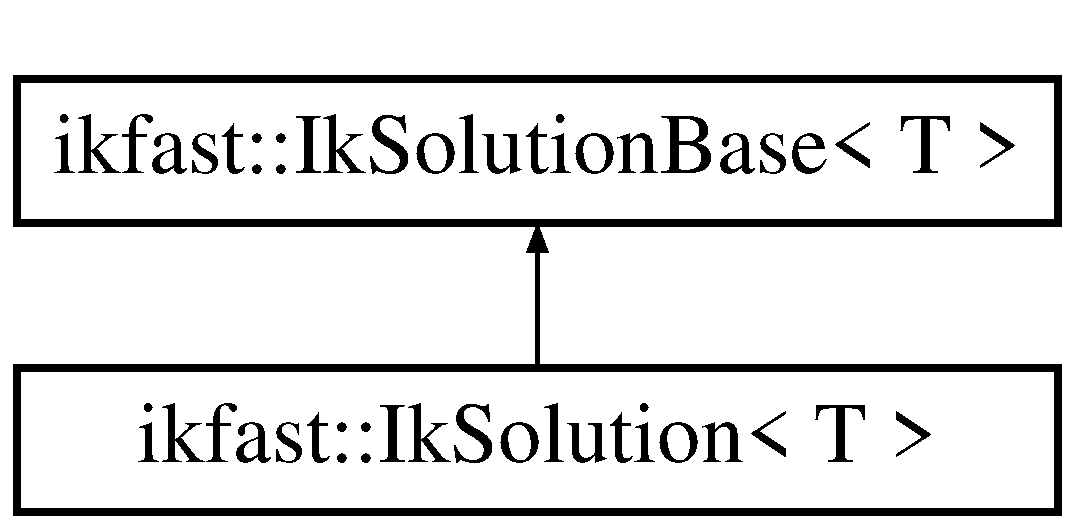
\includegraphics[height=2.000000cm]{classikfast_1_1IkSolution}
\end{center}
\end{figure}
\subsection*{Public Member Functions}
\begin{DoxyCompactItemize}
\item 
\hyperlink{classikfast_1_1IkSolution_a6b76af506a24ba4b78b1c9d3dc110a72}{Ik\-Solution} (const std\-::vector$<$ \hyperlink{classikfast_1_1IkSingleDOFSolutionBase}{Ik\-Single\-D\-O\-F\-Solution\-Base}$<$ T $>$ $>$ \&vinfos, const std\-::vector$<$ int $>$ \&vfree)
\item 
virtual void \hyperlink{classikfast_1_1IkSolution_a197868105dffb498bec69c38318283a2}{Get\-Solution} (T $\ast$solution, const T $\ast$freevalues) const 
\item 
virtual void \hyperlink{classikfast_1_1IkSolution_a56a7305f2111808478f85a43ecc5e6aa}{Get\-Solution} (std\-::vector$<$ T $>$ \&solution, const std\-::vector$<$ T $>$ \&freevalues) const 
\item 
virtual const std\-::vector$<$ int $>$ \& \hyperlink{classikfast_1_1IkSolution_a31267c02ff31436b0bfe3672bcecce5e}{Get\-Free} () const 
\item 
virtual const int \hyperlink{classikfast_1_1IkSolution_a8d46fe7ed5a582f9ad3f4bfc86b41297}{Get\-D\-O\-F} () const 
\item 
virtual void \hyperlink{classikfast_1_1IkSolution_ad61847499fe76751629f70047f8b0a69}{Validate} () const 
\item 
virtual void \hyperlink{classikfast_1_1IkSolution_ae6b77cab94b40369712a099cc21d42e8}{Get\-Solution\-Indices} (std\-::vector$<$ unsigned int $>$ \&v) const 
\end{DoxyCompactItemize}
\subsection*{Public Attributes}
\begin{DoxyCompactItemize}
\item 
std\-::vector\\*
$<$ \hyperlink{classikfast_1_1IkSingleDOFSolutionBase}{Ik\-Single\-D\-O\-F\-Solution\-Base}$<$ T $>$ $>$ \hyperlink{classikfast_1_1IkSolution_a823a44ea0a199929967ce1646792a50c}{\-\_\-vbasesol}
\item 
std\-::vector$<$ int $>$ \hyperlink{classikfast_1_1IkSolution_a3c552543a66e39e127bed5a5c085b1bb}{\-\_\-vfree}
\end{DoxyCompactItemize}


\subsection{Constructor \& Destructor Documentation}
\hypertarget{classikfast_1_1IkSolution_a6b76af506a24ba4b78b1c9d3dc110a72}{\index{ikfast\-::\-Ik\-Solution@{ikfast\-::\-Ik\-Solution}!Ik\-Solution@{Ik\-Solution}}
\index{Ik\-Solution@{Ik\-Solution}!ikfast::IkSolution@{ikfast\-::\-Ik\-Solution}}
\subsubsection[{Ik\-Solution}]{\setlength{\rightskip}{0pt plus 5cm}template$<$typename T $>$ {\bf ikfast\-::\-Ik\-Solution}$<$ T $>$\-::{\bf Ik\-Solution} (
\begin{DoxyParamCaption}
\item[{const std\-::vector$<$ {\bf Ik\-Single\-D\-O\-F\-Solution\-Base}$<$ T $>$ $>$ \&}]{vinfos, }
\item[{const std\-::vector$<$ int $>$ \&}]{vfree}
\end{DoxyParamCaption}
)\hspace{0.3cm}{\ttfamily [inline]}}}\label{classikfast_1_1IkSolution_a6b76af506a24ba4b78b1c9d3dc110a72}


\subsection{Member Function Documentation}
\hypertarget{classikfast_1_1IkSolution_a8d46fe7ed5a582f9ad3f4bfc86b41297}{\index{ikfast\-::\-Ik\-Solution@{ikfast\-::\-Ik\-Solution}!Get\-D\-O\-F@{Get\-D\-O\-F}}
\index{Get\-D\-O\-F@{Get\-D\-O\-F}!ikfast::IkSolution@{ikfast\-::\-Ik\-Solution}}
\subsubsection[{Get\-D\-O\-F}]{\setlength{\rightskip}{0pt plus 5cm}template$<$typename T $>$ virtual const int {\bf ikfast\-::\-Ik\-Solution}$<$ T $>$\-::Get\-D\-O\-F (
\begin{DoxyParamCaption}
{}
\end{DoxyParamCaption}
) const\hspace{0.3cm}{\ttfamily [inline]}, {\ttfamily [virtual]}}}\label{classikfast_1_1IkSolution_a8d46fe7ed5a582f9ad3f4bfc86b41297}


Implements \hyperlink{classikfast_1_1IkSolutionBase_aac54f54aa69b27991651b0ba2a21208c}{ikfast\-::\-Ik\-Solution\-Base$<$ T $>$}.

\hypertarget{classikfast_1_1IkSolution_a31267c02ff31436b0bfe3672bcecce5e}{\index{ikfast\-::\-Ik\-Solution@{ikfast\-::\-Ik\-Solution}!Get\-Free@{Get\-Free}}
\index{Get\-Free@{Get\-Free}!ikfast::IkSolution@{ikfast\-::\-Ik\-Solution}}
\subsubsection[{Get\-Free}]{\setlength{\rightskip}{0pt plus 5cm}template$<$typename T $>$ virtual const std\-::vector$<$int$>$\& {\bf ikfast\-::\-Ik\-Solution}$<$ T $>$\-::Get\-Free (
\begin{DoxyParamCaption}
{}
\end{DoxyParamCaption}
) const\hspace{0.3cm}{\ttfamily [inline]}, {\ttfamily [virtual]}}}\label{classikfast_1_1IkSolution_a31267c02ff31436b0bfe3672bcecce5e}


Implements \hyperlink{classikfast_1_1IkSolutionBase_a2693ede66be937b7c4c1c949284282ca}{ikfast\-::\-Ik\-Solution\-Base$<$ T $>$}.

\hypertarget{classikfast_1_1IkSolution_a197868105dffb498bec69c38318283a2}{\index{ikfast\-::\-Ik\-Solution@{ikfast\-::\-Ik\-Solution}!Get\-Solution@{Get\-Solution}}
\index{Get\-Solution@{Get\-Solution}!ikfast::IkSolution@{ikfast\-::\-Ik\-Solution}}
\subsubsection[{Get\-Solution}]{\setlength{\rightskip}{0pt plus 5cm}template$<$typename T $>$ virtual void {\bf ikfast\-::\-Ik\-Solution}$<$ T $>$\-::Get\-Solution (
\begin{DoxyParamCaption}
\item[{T $\ast$}]{solution, }
\item[{const T $\ast$}]{freevalues}
\end{DoxyParamCaption}
) const\hspace{0.3cm}{\ttfamily [inline]}, {\ttfamily [virtual]}}}\label{classikfast_1_1IkSolution_a197868105dffb498bec69c38318283a2}


Implements \hyperlink{classikfast_1_1IkSolutionBase_a9405530feb49f12f56c3175e7150c66f}{ikfast\-::\-Ik\-Solution\-Base$<$ T $>$}.

\hypertarget{classikfast_1_1IkSolution_a56a7305f2111808478f85a43ecc5e6aa}{\index{ikfast\-::\-Ik\-Solution@{ikfast\-::\-Ik\-Solution}!Get\-Solution@{Get\-Solution}}
\index{Get\-Solution@{Get\-Solution}!ikfast::IkSolution@{ikfast\-::\-Ik\-Solution}}
\subsubsection[{Get\-Solution}]{\setlength{\rightskip}{0pt plus 5cm}template$<$typename T $>$ virtual void {\bf ikfast\-::\-Ik\-Solution}$<$ T $>$\-::Get\-Solution (
\begin{DoxyParamCaption}
\item[{std\-::vector$<$ T $>$ \&}]{solution, }
\item[{const std\-::vector$<$ T $>$ \&}]{freevalues}
\end{DoxyParamCaption}
) const\hspace{0.3cm}{\ttfamily [inline]}, {\ttfamily [virtual]}}}\label{classikfast_1_1IkSolution_a56a7305f2111808478f85a43ecc5e6aa}


Reimplemented from \hyperlink{classikfast_1_1IkSolutionBase_a2b558f7a29be0868cff3e81fbd9594c4}{ikfast\-::\-Ik\-Solution\-Base$<$ T $>$}.

\hypertarget{classikfast_1_1IkSolution_ae6b77cab94b40369712a099cc21d42e8}{\index{ikfast\-::\-Ik\-Solution@{ikfast\-::\-Ik\-Solution}!Get\-Solution\-Indices@{Get\-Solution\-Indices}}
\index{Get\-Solution\-Indices@{Get\-Solution\-Indices}!ikfast::IkSolution@{ikfast\-::\-Ik\-Solution}}
\subsubsection[{Get\-Solution\-Indices}]{\setlength{\rightskip}{0pt plus 5cm}template$<$typename T $>$ virtual void {\bf ikfast\-::\-Ik\-Solution}$<$ T $>$\-::Get\-Solution\-Indices (
\begin{DoxyParamCaption}
\item[{std\-::vector$<$ unsigned int $>$ \&}]{v}
\end{DoxyParamCaption}
) const\hspace{0.3cm}{\ttfamily [inline]}, {\ttfamily [virtual]}}}\label{classikfast_1_1IkSolution_ae6b77cab94b40369712a099cc21d42e8}
\hypertarget{classikfast_1_1IkSolution_ad61847499fe76751629f70047f8b0a69}{\index{ikfast\-::\-Ik\-Solution@{ikfast\-::\-Ik\-Solution}!Validate@{Validate}}
\index{Validate@{Validate}!ikfast::IkSolution@{ikfast\-::\-Ik\-Solution}}
\subsubsection[{Validate}]{\setlength{\rightskip}{0pt plus 5cm}template$<$typename T $>$ virtual void {\bf ikfast\-::\-Ik\-Solution}$<$ T $>$\-::Validate (
\begin{DoxyParamCaption}
{}
\end{DoxyParamCaption}
) const\hspace{0.3cm}{\ttfamily [inline]}, {\ttfamily [virtual]}}}\label{classikfast_1_1IkSolution_ad61847499fe76751629f70047f8b0a69}


\subsection{Member Data Documentation}
\hypertarget{classikfast_1_1IkSolution_a823a44ea0a199929967ce1646792a50c}{\index{ikfast\-::\-Ik\-Solution@{ikfast\-::\-Ik\-Solution}!\-\_\-vbasesol@{\-\_\-vbasesol}}
\index{\-\_\-vbasesol@{\-\_\-vbasesol}!ikfast::IkSolution@{ikfast\-::\-Ik\-Solution}}
\subsubsection[{\-\_\-vbasesol}]{\setlength{\rightskip}{0pt plus 5cm}template$<$typename T $>$ std\-::vector$<${\bf Ik\-Single\-D\-O\-F\-Solution\-Base}$<$T$>$ $>$ {\bf ikfast\-::\-Ik\-Solution}$<$ T $>$\-::\-\_\-vbasesol}}\label{classikfast_1_1IkSolution_a823a44ea0a199929967ce1646792a50c}
\hypertarget{classikfast_1_1IkSolution_a3c552543a66e39e127bed5a5c085b1bb}{\index{ikfast\-::\-Ik\-Solution@{ikfast\-::\-Ik\-Solution}!\-\_\-vfree@{\-\_\-vfree}}
\index{\-\_\-vfree@{\-\_\-vfree}!ikfast::IkSolution@{ikfast\-::\-Ik\-Solution}}
\subsubsection[{\-\_\-vfree}]{\setlength{\rightskip}{0pt plus 5cm}template$<$typename T $>$ std\-::vector$<$int$>$ {\bf ikfast\-::\-Ik\-Solution}$<$ T $>$\-::\-\_\-vfree}}\label{classikfast_1_1IkSolution_a3c552543a66e39e127bed5a5c085b1bb}


The documentation for this class was generated from the following file\-:\begin{DoxyCompactItemize}
\item 
/usr/local/michalos/nistfanuc\-\_\-ws/src/nist\-\_\-fanuc/include/nist\-\_\-fanuc/\hyperlink{ikfast_8h}{ikfast.\-h}\end{DoxyCompactItemize}

\hypertarget{classikfast_1_1IkSolutionBase}{\section{ikfast\-:\-:Ik\-Solution\-Base$<$ T $>$ Class Template Reference}
\label{classikfast_1_1IkSolutionBase}\index{ikfast\-::\-Ik\-Solution\-Base$<$ T $>$@{ikfast\-::\-Ik\-Solution\-Base$<$ T $>$}}
}


{\ttfamily \#include $<$ikfast.\-h$>$}

Inheritance diagram for ikfast\-:\-:Ik\-Solution\-Base$<$ T $>$\-:\begin{figure}[H]
\begin{center}
\leavevmode
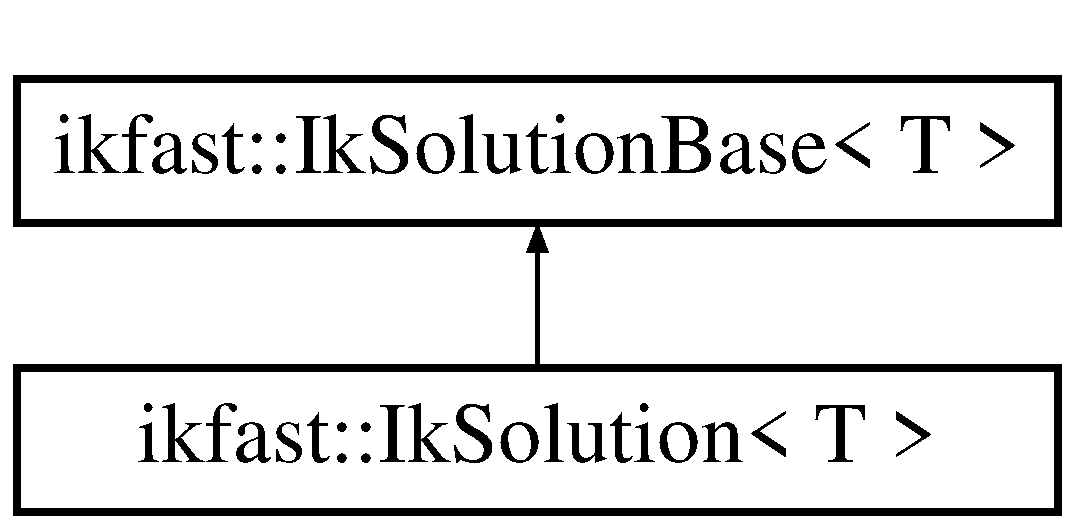
\includegraphics[height=2.000000cm]{classikfast_1_1IkSolutionBase}
\end{center}
\end{figure}
\subsection*{Public Member Functions}
\begin{DoxyCompactItemize}
\item 
virtual \hyperlink{classikfast_1_1IkSolutionBase_ae40e464cdbc474388cc7d55560ec44f9}{$\sim$\-Ik\-Solution\-Base} ()
\item 
virtual void \hyperlink{classikfast_1_1IkSolutionBase_a9405530feb49f12f56c3175e7150c66f}{Get\-Solution} (T $\ast$solution, const T $\ast$freevalues) const =0
\item 
virtual void \hyperlink{classikfast_1_1IkSolutionBase_a2b558f7a29be0868cff3e81fbd9594c4}{Get\-Solution} (std\-::vector$<$ T $>$ \&solution, const std\-::vector$<$ T $>$ \&freevalues) const 
\item 
virtual const std\-::vector$<$ int $>$ \& \hyperlink{classikfast_1_1IkSolutionBase_a2693ede66be937b7c4c1c949284282ca}{Get\-Free} () const =0
\item 
virtual const int \hyperlink{classikfast_1_1IkSolutionBase_aac54f54aa69b27991651b0ba2a21208c}{Get\-D\-O\-F} () const =0
\end{DoxyCompactItemize}


\subsection{Constructor \& Destructor Documentation}
\hypertarget{classikfast_1_1IkSolutionBase_ae40e464cdbc474388cc7d55560ec44f9}{\index{ikfast\-::\-Ik\-Solution\-Base@{ikfast\-::\-Ik\-Solution\-Base}!$\sim$\-Ik\-Solution\-Base@{$\sim$\-Ik\-Solution\-Base}}
\index{$\sim$\-Ik\-Solution\-Base@{$\sim$\-Ik\-Solution\-Base}!ikfast::IkSolutionBase@{ikfast\-::\-Ik\-Solution\-Base}}
\subsubsection[{$\sim$\-Ik\-Solution\-Base}]{\setlength{\rightskip}{0pt plus 5cm}template$<$typename T$>$ virtual {\bf ikfast\-::\-Ik\-Solution\-Base}$<$ T $>$\-::$\sim${\bf Ik\-Solution\-Base} (
\begin{DoxyParamCaption}
{}
\end{DoxyParamCaption}
)\hspace{0.3cm}{\ttfamily [inline]}, {\ttfamily [virtual]}}}\label{classikfast_1_1IkSolutionBase_ae40e464cdbc474388cc7d55560ec44f9}


\subsection{Member Function Documentation}
\hypertarget{classikfast_1_1IkSolutionBase_aac54f54aa69b27991651b0ba2a21208c}{\index{ikfast\-::\-Ik\-Solution\-Base@{ikfast\-::\-Ik\-Solution\-Base}!Get\-D\-O\-F@{Get\-D\-O\-F}}
\index{Get\-D\-O\-F@{Get\-D\-O\-F}!ikfast::IkSolutionBase@{ikfast\-::\-Ik\-Solution\-Base}}
\subsubsection[{Get\-D\-O\-F}]{\setlength{\rightskip}{0pt plus 5cm}template$<$typename T$>$ virtual const int {\bf ikfast\-::\-Ik\-Solution\-Base}$<$ T $>$\-::Get\-D\-O\-F (
\begin{DoxyParamCaption}
{}
\end{DoxyParamCaption}
) const\hspace{0.3cm}{\ttfamily [pure virtual]}}}\label{classikfast_1_1IkSolutionBase_aac54f54aa69b27991651b0ba2a21208c}


Implemented in \hyperlink{classikfast_1_1IkSolution_a8d46fe7ed5a582f9ad3f4bfc86b41297}{ikfast\-::\-Ik\-Solution$<$ T $>$}.

\hypertarget{classikfast_1_1IkSolutionBase_a2693ede66be937b7c4c1c949284282ca}{\index{ikfast\-::\-Ik\-Solution\-Base@{ikfast\-::\-Ik\-Solution\-Base}!Get\-Free@{Get\-Free}}
\index{Get\-Free@{Get\-Free}!ikfast::IkSolutionBase@{ikfast\-::\-Ik\-Solution\-Base}}
\subsubsection[{Get\-Free}]{\setlength{\rightskip}{0pt plus 5cm}template$<$typename T$>$ virtual const std\-::vector$<$int$>$\& {\bf ikfast\-::\-Ik\-Solution\-Base}$<$ T $>$\-::Get\-Free (
\begin{DoxyParamCaption}
{}
\end{DoxyParamCaption}
) const\hspace{0.3cm}{\ttfamily [pure virtual]}}}\label{classikfast_1_1IkSolutionBase_a2693ede66be937b7c4c1c949284282ca}


Implemented in \hyperlink{classikfast_1_1IkSolution_a31267c02ff31436b0bfe3672bcecce5e}{ikfast\-::\-Ik\-Solution$<$ T $>$}.

\hypertarget{classikfast_1_1IkSolutionBase_a9405530feb49f12f56c3175e7150c66f}{\index{ikfast\-::\-Ik\-Solution\-Base@{ikfast\-::\-Ik\-Solution\-Base}!Get\-Solution@{Get\-Solution}}
\index{Get\-Solution@{Get\-Solution}!ikfast::IkSolutionBase@{ikfast\-::\-Ik\-Solution\-Base}}
\subsubsection[{Get\-Solution}]{\setlength{\rightskip}{0pt plus 5cm}template$<$typename T$>$ virtual void {\bf ikfast\-::\-Ik\-Solution\-Base}$<$ T $>$\-::Get\-Solution (
\begin{DoxyParamCaption}
\item[{T $\ast$}]{solution, }
\item[{const T $\ast$}]{freevalues}
\end{DoxyParamCaption}
) const\hspace{0.3cm}{\ttfamily [pure virtual]}}}\label{classikfast_1_1IkSolutionBase_a9405530feb49f12f56c3175e7150c66f}


Implemented in \hyperlink{classikfast_1_1IkSolution_a197868105dffb498bec69c38318283a2}{ikfast\-::\-Ik\-Solution$<$ T $>$}.

\hypertarget{classikfast_1_1IkSolutionBase_a2b558f7a29be0868cff3e81fbd9594c4}{\index{ikfast\-::\-Ik\-Solution\-Base@{ikfast\-::\-Ik\-Solution\-Base}!Get\-Solution@{Get\-Solution}}
\index{Get\-Solution@{Get\-Solution}!ikfast::IkSolutionBase@{ikfast\-::\-Ik\-Solution\-Base}}
\subsubsection[{Get\-Solution}]{\setlength{\rightskip}{0pt plus 5cm}template$<$typename T$>$ virtual void {\bf ikfast\-::\-Ik\-Solution\-Base}$<$ T $>$\-::Get\-Solution (
\begin{DoxyParamCaption}
\item[{std\-::vector$<$ T $>$ \&}]{solution, }
\item[{const std\-::vector$<$ T $>$ \&}]{freevalues}
\end{DoxyParamCaption}
) const\hspace{0.3cm}{\ttfamily [inline]}, {\ttfamily [virtual]}}}\label{classikfast_1_1IkSolutionBase_a2b558f7a29be0868cff3e81fbd9594c4}


Reimplemented in \hyperlink{classikfast_1_1IkSolution_a56a7305f2111808478f85a43ecc5e6aa}{ikfast\-::\-Ik\-Solution$<$ T $>$}.



The documentation for this class was generated from the following file\-:\begin{DoxyCompactItemize}
\item 
/usr/local/michalos/nistfanuc\-\_\-ws/src/nist\-\_\-fanuc/include/nist\-\_\-fanuc/\hyperlink{ikfast_8h}{ikfast.\-h}\end{DoxyCompactItemize}

\hypertarget{classikfast_1_1IkSolutionList}{\section{ikfast\-:\-:Ik\-Solution\-List$<$ T $>$ Class Template Reference}
\label{classikfast_1_1IkSolutionList}\index{ikfast\-::\-Ik\-Solution\-List$<$ T $>$@{ikfast\-::\-Ik\-Solution\-List$<$ T $>$}}
}


{\ttfamily \#include $<$ikfast.\-h$>$}

Inheritance diagram for ikfast\-:\-:Ik\-Solution\-List$<$ T $>$\-:\begin{figure}[H]
\begin{center}
\leavevmode
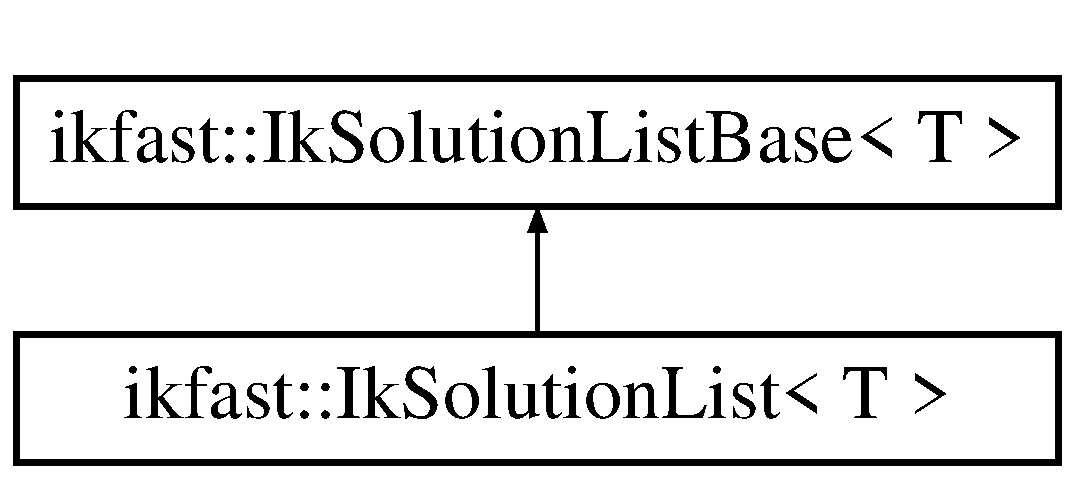
\includegraphics[height=2.000000cm]{classikfast_1_1IkSolutionList}
\end{center}
\end{figure}
\subsection*{Public Member Functions}
\begin{DoxyCompactItemize}
\item 
virtual size\-\_\-t \hyperlink{classikfast_1_1IkSolutionList_ac0a503b13e68403e7b2d92afd4c28a7b}{Add\-Solution} (const std\-::vector$<$ \hyperlink{classikfast_1_1IkSingleDOFSolutionBase}{Ik\-Single\-D\-O\-F\-Solution\-Base}$<$ T $>$ $>$ \&vinfos, const std\-::vector$<$ int $>$ \&vfree)
\item 
virtual const \hyperlink{classikfast_1_1IkSolutionBase}{Ik\-Solution\-Base}$<$ T $>$ \& \hyperlink{classikfast_1_1IkSolutionList_ab2840cca4cea5547d684907047d38bba}{Get\-Solution} (size\-\_\-t index) const 
\item 
virtual size\-\_\-t \hyperlink{classikfast_1_1IkSolutionList_a4508235ea7738ee067d6525a34362567}{Get\-Num\-Solutions} () const 
\item 
virtual void \hyperlink{classikfast_1_1IkSolutionList_ae341a33d5aee644cac867e3edd2a9916}{Clear} ()
\end{DoxyCompactItemize}
\subsection*{Protected Attributes}
\begin{DoxyCompactItemize}
\item 
std\-::list$<$ \hyperlink{classikfast_1_1IkSolution}{Ik\-Solution}$<$ T $>$ $>$ \hyperlink{classikfast_1_1IkSolutionList_a141004e6be454a5b9ab537d102c7f405}{\-\_\-listsolutions}
\end{DoxyCompactItemize}


\subsection{Member Function Documentation}
\hypertarget{classikfast_1_1IkSolutionList_ac0a503b13e68403e7b2d92afd4c28a7b}{\index{ikfast\-::\-Ik\-Solution\-List@{ikfast\-::\-Ik\-Solution\-List}!Add\-Solution@{Add\-Solution}}
\index{Add\-Solution@{Add\-Solution}!ikfast::IkSolutionList@{ikfast\-::\-Ik\-Solution\-List}}
\subsubsection[{Add\-Solution}]{\setlength{\rightskip}{0pt plus 5cm}template$<$typename T$>$ virtual size\-\_\-t {\bf ikfast\-::\-Ik\-Solution\-List}$<$ T $>$\-::Add\-Solution (
\begin{DoxyParamCaption}
\item[{const std\-::vector$<$ {\bf Ik\-Single\-D\-O\-F\-Solution\-Base}$<$ T $>$ $>$ \&}]{vinfos, }
\item[{const std\-::vector$<$ int $>$ \&}]{vfree}
\end{DoxyParamCaption}
)\hspace{0.3cm}{\ttfamily [inline]}, {\ttfamily [virtual]}}}\label{classikfast_1_1IkSolutionList_ac0a503b13e68403e7b2d92afd4c28a7b}


Implements \hyperlink{classikfast_1_1IkSolutionListBase_a9d862f550472c2fa15189946b12222bf}{ikfast\-::\-Ik\-Solution\-List\-Base$<$ T $>$}.

\hypertarget{classikfast_1_1IkSolutionList_ae341a33d5aee644cac867e3edd2a9916}{\index{ikfast\-::\-Ik\-Solution\-List@{ikfast\-::\-Ik\-Solution\-List}!Clear@{Clear}}
\index{Clear@{Clear}!ikfast::IkSolutionList@{ikfast\-::\-Ik\-Solution\-List}}
\subsubsection[{Clear}]{\setlength{\rightskip}{0pt plus 5cm}template$<$typename T$>$ virtual void {\bf ikfast\-::\-Ik\-Solution\-List}$<$ T $>$\-::Clear (
\begin{DoxyParamCaption}
{}
\end{DoxyParamCaption}
)\hspace{0.3cm}{\ttfamily [inline]}, {\ttfamily [virtual]}}}\label{classikfast_1_1IkSolutionList_ae341a33d5aee644cac867e3edd2a9916}


Implements \hyperlink{classikfast_1_1IkSolutionListBase_a9940fe21cfa0a67c1a21a672696c5cb5}{ikfast\-::\-Ik\-Solution\-List\-Base$<$ T $>$}.

\hypertarget{classikfast_1_1IkSolutionList_a4508235ea7738ee067d6525a34362567}{\index{ikfast\-::\-Ik\-Solution\-List@{ikfast\-::\-Ik\-Solution\-List}!Get\-Num\-Solutions@{Get\-Num\-Solutions}}
\index{Get\-Num\-Solutions@{Get\-Num\-Solutions}!ikfast::IkSolutionList@{ikfast\-::\-Ik\-Solution\-List}}
\subsubsection[{Get\-Num\-Solutions}]{\setlength{\rightskip}{0pt plus 5cm}template$<$typename T$>$ virtual size\-\_\-t {\bf ikfast\-::\-Ik\-Solution\-List}$<$ T $>$\-::Get\-Num\-Solutions (
\begin{DoxyParamCaption}
{}
\end{DoxyParamCaption}
) const\hspace{0.3cm}{\ttfamily [inline]}, {\ttfamily [virtual]}}}\label{classikfast_1_1IkSolutionList_a4508235ea7738ee067d6525a34362567}


Implements \hyperlink{classikfast_1_1IkSolutionListBase_a5f4a2191825f1d2aad3468daf94d575f}{ikfast\-::\-Ik\-Solution\-List\-Base$<$ T $>$}.

\hypertarget{classikfast_1_1IkSolutionList_ab2840cca4cea5547d684907047d38bba}{\index{ikfast\-::\-Ik\-Solution\-List@{ikfast\-::\-Ik\-Solution\-List}!Get\-Solution@{Get\-Solution}}
\index{Get\-Solution@{Get\-Solution}!ikfast::IkSolutionList@{ikfast\-::\-Ik\-Solution\-List}}
\subsubsection[{Get\-Solution}]{\setlength{\rightskip}{0pt plus 5cm}template$<$typename T$>$ virtual const {\bf Ik\-Solution\-Base}$<$T$>$\& {\bf ikfast\-::\-Ik\-Solution\-List}$<$ T $>$\-::Get\-Solution (
\begin{DoxyParamCaption}
\item[{size\-\_\-t}]{index}
\end{DoxyParamCaption}
) const\hspace{0.3cm}{\ttfamily [inline]}, {\ttfamily [virtual]}}}\label{classikfast_1_1IkSolutionList_ab2840cca4cea5547d684907047d38bba}


Implements \hyperlink{classikfast_1_1IkSolutionListBase_a540d8c85b5be635ea671ef7ddc0eb9c0}{ikfast\-::\-Ik\-Solution\-List\-Base$<$ T $>$}.



\subsection{Member Data Documentation}
\hypertarget{classikfast_1_1IkSolutionList_a141004e6be454a5b9ab537d102c7f405}{\index{ikfast\-::\-Ik\-Solution\-List@{ikfast\-::\-Ik\-Solution\-List}!\-\_\-listsolutions@{\-\_\-listsolutions}}
\index{\-\_\-listsolutions@{\-\_\-listsolutions}!ikfast::IkSolutionList@{ikfast\-::\-Ik\-Solution\-List}}
\subsubsection[{\-\_\-listsolutions}]{\setlength{\rightskip}{0pt plus 5cm}template$<$typename T$>$ std\-::list$<${\bf Ik\-Solution}$<$T$>$ $>$ {\bf ikfast\-::\-Ik\-Solution\-List}$<$ T $>$\-::\-\_\-listsolutions\hspace{0.3cm}{\ttfamily [protected]}}}\label{classikfast_1_1IkSolutionList_a141004e6be454a5b9ab537d102c7f405}


The documentation for this class was generated from the following file\-:\begin{DoxyCompactItemize}
\item 
/usr/local/michalos/nistfanuc\-\_\-ws/src/nist\-\_\-fanuc/include/nist\-\_\-fanuc/\hyperlink{ikfast_8h}{ikfast.\-h}\end{DoxyCompactItemize}

\hypertarget{classikfast_1_1IkSolutionListBase}{\section{ikfast\-:\-:Ik\-Solution\-List\-Base$<$ T $>$ Class Template Reference}
\label{classikfast_1_1IkSolutionListBase}\index{ikfast\-::\-Ik\-Solution\-List\-Base$<$ T $>$@{ikfast\-::\-Ik\-Solution\-List\-Base$<$ T $>$}}
}


{\ttfamily \#include $<$ikfast.\-h$>$}

Inheritance diagram for ikfast\-:\-:Ik\-Solution\-List\-Base$<$ T $>$\-:\begin{figure}[H]
\begin{center}
\leavevmode
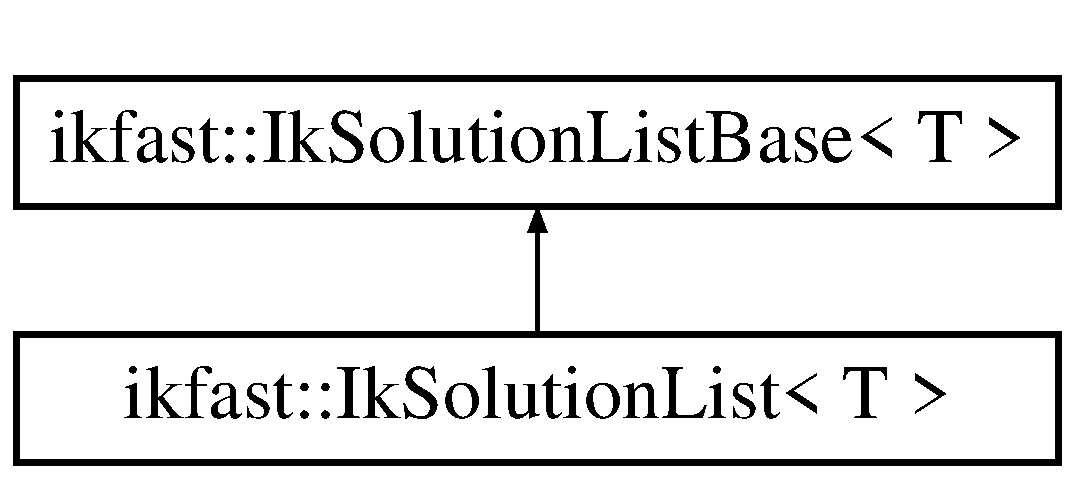
\includegraphics[height=2.000000cm]{classikfast_1_1IkSolutionListBase}
\end{center}
\end{figure}
\subsection*{Public Member Functions}
\begin{DoxyCompactItemize}
\item 
virtual \hyperlink{classikfast_1_1IkSolutionListBase_a1200afc2fc92110d9f8191039f0f7d6c}{$\sim$\-Ik\-Solution\-List\-Base} ()
\item 
virtual size\-\_\-t \hyperlink{classikfast_1_1IkSolutionListBase_a9d862f550472c2fa15189946b12222bf}{Add\-Solution} (const std\-::vector$<$ \hyperlink{classikfast_1_1IkSingleDOFSolutionBase}{Ik\-Single\-D\-O\-F\-Solution\-Base}$<$ T $>$ $>$ \&vinfos, const std\-::vector$<$ int $>$ \&vfree)=0
\item 
virtual const \hyperlink{classikfast_1_1IkSolutionBase}{Ik\-Solution\-Base}$<$ T $>$ \& \hyperlink{classikfast_1_1IkSolutionListBase_a540d8c85b5be635ea671ef7ddc0eb9c0}{Get\-Solution} (size\-\_\-t index) const =0
\item 
virtual size\-\_\-t \hyperlink{classikfast_1_1IkSolutionListBase_a5f4a2191825f1d2aad3468daf94d575f}{Get\-Num\-Solutions} () const =0
\item 
virtual void \hyperlink{classikfast_1_1IkSolutionListBase_a9940fe21cfa0a67c1a21a672696c5cb5}{Clear} ()=0
\end{DoxyCompactItemize}


\subsection{Constructor \& Destructor Documentation}
\hypertarget{classikfast_1_1IkSolutionListBase_a1200afc2fc92110d9f8191039f0f7d6c}{\index{ikfast\-::\-Ik\-Solution\-List\-Base@{ikfast\-::\-Ik\-Solution\-List\-Base}!$\sim$\-Ik\-Solution\-List\-Base@{$\sim$\-Ik\-Solution\-List\-Base}}
\index{$\sim$\-Ik\-Solution\-List\-Base@{$\sim$\-Ik\-Solution\-List\-Base}!ikfast::IkSolutionListBase@{ikfast\-::\-Ik\-Solution\-List\-Base}}
\subsubsection[{$\sim$\-Ik\-Solution\-List\-Base}]{\setlength{\rightskip}{0pt plus 5cm}template$<$typename T$>$ virtual {\bf ikfast\-::\-Ik\-Solution\-List\-Base}$<$ T $>$\-::$\sim${\bf Ik\-Solution\-List\-Base} (
\begin{DoxyParamCaption}
{}
\end{DoxyParamCaption}
)\hspace{0.3cm}{\ttfamily [inline]}, {\ttfamily [virtual]}}}\label{classikfast_1_1IkSolutionListBase_a1200afc2fc92110d9f8191039f0f7d6c}


\subsection{Member Function Documentation}
\hypertarget{classikfast_1_1IkSolutionListBase_a9d862f550472c2fa15189946b12222bf}{\index{ikfast\-::\-Ik\-Solution\-List\-Base@{ikfast\-::\-Ik\-Solution\-List\-Base}!Add\-Solution@{Add\-Solution}}
\index{Add\-Solution@{Add\-Solution}!ikfast::IkSolutionListBase@{ikfast\-::\-Ik\-Solution\-List\-Base}}
\subsubsection[{Add\-Solution}]{\setlength{\rightskip}{0pt plus 5cm}template$<$typename T$>$ virtual size\-\_\-t {\bf ikfast\-::\-Ik\-Solution\-List\-Base}$<$ T $>$\-::Add\-Solution (
\begin{DoxyParamCaption}
\item[{const std\-::vector$<$ {\bf Ik\-Single\-D\-O\-F\-Solution\-Base}$<$ T $>$ $>$ \&}]{vinfos, }
\item[{const std\-::vector$<$ int $>$ \&}]{vfree}
\end{DoxyParamCaption}
)\hspace{0.3cm}{\ttfamily [pure virtual]}}}\label{classikfast_1_1IkSolutionListBase_a9d862f550472c2fa15189946b12222bf}


Implemented in \hyperlink{classikfast_1_1IkSolutionList_ac0a503b13e68403e7b2d92afd4c28a7b}{ikfast\-::\-Ik\-Solution\-List$<$ T $>$}.

\hypertarget{classikfast_1_1IkSolutionListBase_a9940fe21cfa0a67c1a21a672696c5cb5}{\index{ikfast\-::\-Ik\-Solution\-List\-Base@{ikfast\-::\-Ik\-Solution\-List\-Base}!Clear@{Clear}}
\index{Clear@{Clear}!ikfast::IkSolutionListBase@{ikfast\-::\-Ik\-Solution\-List\-Base}}
\subsubsection[{Clear}]{\setlength{\rightskip}{0pt plus 5cm}template$<$typename T$>$ virtual void {\bf ikfast\-::\-Ik\-Solution\-List\-Base}$<$ T $>$\-::Clear (
\begin{DoxyParamCaption}
{}
\end{DoxyParamCaption}
)\hspace{0.3cm}{\ttfamily [pure virtual]}}}\label{classikfast_1_1IkSolutionListBase_a9940fe21cfa0a67c1a21a672696c5cb5}


Implemented in \hyperlink{classikfast_1_1IkSolutionList_ae341a33d5aee644cac867e3edd2a9916}{ikfast\-::\-Ik\-Solution\-List$<$ T $>$}.

\hypertarget{classikfast_1_1IkSolutionListBase_a5f4a2191825f1d2aad3468daf94d575f}{\index{ikfast\-::\-Ik\-Solution\-List\-Base@{ikfast\-::\-Ik\-Solution\-List\-Base}!Get\-Num\-Solutions@{Get\-Num\-Solutions}}
\index{Get\-Num\-Solutions@{Get\-Num\-Solutions}!ikfast::IkSolutionListBase@{ikfast\-::\-Ik\-Solution\-List\-Base}}
\subsubsection[{Get\-Num\-Solutions}]{\setlength{\rightskip}{0pt plus 5cm}template$<$typename T$>$ virtual size\-\_\-t {\bf ikfast\-::\-Ik\-Solution\-List\-Base}$<$ T $>$\-::Get\-Num\-Solutions (
\begin{DoxyParamCaption}
{}
\end{DoxyParamCaption}
) const\hspace{0.3cm}{\ttfamily [pure virtual]}}}\label{classikfast_1_1IkSolutionListBase_a5f4a2191825f1d2aad3468daf94d575f}


Implemented in \hyperlink{classikfast_1_1IkSolutionList_a4508235ea7738ee067d6525a34362567}{ikfast\-::\-Ik\-Solution\-List$<$ T $>$}.

\hypertarget{classikfast_1_1IkSolutionListBase_a540d8c85b5be635ea671ef7ddc0eb9c0}{\index{ikfast\-::\-Ik\-Solution\-List\-Base@{ikfast\-::\-Ik\-Solution\-List\-Base}!Get\-Solution@{Get\-Solution}}
\index{Get\-Solution@{Get\-Solution}!ikfast::IkSolutionListBase@{ikfast\-::\-Ik\-Solution\-List\-Base}}
\subsubsection[{Get\-Solution}]{\setlength{\rightskip}{0pt plus 5cm}template$<$typename T$>$ virtual const {\bf Ik\-Solution\-Base}$<$T$>$\& {\bf ikfast\-::\-Ik\-Solution\-List\-Base}$<$ T $>$\-::Get\-Solution (
\begin{DoxyParamCaption}
\item[{size\-\_\-t}]{index}
\end{DoxyParamCaption}
) const\hspace{0.3cm}{\ttfamily [pure virtual]}}}\label{classikfast_1_1IkSolutionListBase_a540d8c85b5be635ea671ef7ddc0eb9c0}


Implemented in \hyperlink{classikfast_1_1IkSolutionList_ab2840cca4cea5547d684907047d38bba}{ikfast\-::\-Ik\-Solution\-List$<$ T $>$}.



The documentation for this class was generated from the following file\-:\begin{DoxyCompactItemize}
\item 
/usr/local/michalos/nistfanuc\-\_\-ws/src/nist\-\_\-fanuc/include/nist\-\_\-fanuc/\hyperlink{ikfast_8h}{ikfast.\-h}\end{DoxyCompactItemize}

\hypertarget{classIKSolver}{\section{I\-K\-Solver Class Reference}
\label{classIKSolver}\index{I\-K\-Solver@{I\-K\-Solver}}
}
\subsection*{Public Member Functions}
\begin{DoxyCompactItemize}
\item 
bool \hyperlink{classIKSolver_ac0195e291bed491b4cb6a68db8199b55}{Compute\-Ik} (const \hyperlink{ikfast_8h_ad067e4244010306f633e94db2645dd6d}{Ik\-Real} $\ast$eetrans, const \hyperlink{ikfast_8h_ad067e4244010306f633e94db2645dd6d}{Ik\-Real} $\ast$eerot, const \hyperlink{ikfast_8h_ad067e4244010306f633e94db2645dd6d}{Ik\-Real} $\ast$pfree, \hyperlink{classikfast_1_1IkSolutionListBase}{Ik\-Solution\-List\-Base}$<$ \hyperlink{ikfast_8h_ad067e4244010306f633e94db2645dd6d}{Ik\-Real} $>$ \&solutions)
\item 
void \hyperlink{classIKSolver_a139a62477d8d27e5a5dace907f0b38b0}{rotationfunction0} (\hyperlink{classikfast_1_1IkSolutionListBase}{Ik\-Solution\-List\-Base}$<$ \hyperlink{ikfast_8h_ad067e4244010306f633e94db2645dd6d}{Ik\-Real} $>$ \&solutions)
\end{DoxyCompactItemize}
\subsection*{Public Attributes}
\begin{DoxyCompactItemize}
\item 
\hyperlink{ikfast_8h_ad067e4244010306f633e94db2645dd6d}{Ik\-Real} \hyperlink{classIKSolver_a57f10792b61e342bc910311172b36488}{j0}
\item 
\hyperlink{ikfast_8h_ad067e4244010306f633e94db2645dd6d}{Ik\-Real} \hyperlink{classIKSolver_aa3c0bd74bcf87573ce608d8039408526}{cj0}
\item 
\hyperlink{ikfast_8h_ad067e4244010306f633e94db2645dd6d}{Ik\-Real} \hyperlink{classIKSolver_a791e2437d1fc1b568b213b0388f97d0a}{sj0}
\item 
\hyperlink{ikfast_8h_ad067e4244010306f633e94db2645dd6d}{Ik\-Real} \hyperlink{classIKSolver_af29aefe604a6957a573f5532a0ae0924}{htj0}
\item 
\hyperlink{ikfast_8h_ad067e4244010306f633e94db2645dd6d}{Ik\-Real} \hyperlink{classIKSolver_abce606fc49166277524525eadfe47f1a}{j1}
\item 
\hyperlink{ikfast_8h_ad067e4244010306f633e94db2645dd6d}{Ik\-Real} \hyperlink{classIKSolver_a2eff4800151517f5c649cb948bad8326}{cj1}
\item 
\hyperlink{ikfast_8h_ad067e4244010306f633e94db2645dd6d}{Ik\-Real} \hyperlink{classIKSolver_a0d7c3270795003a7947ae93ba90b8335}{sj1}
\item 
\hyperlink{ikfast_8h_ad067e4244010306f633e94db2645dd6d}{Ik\-Real} \hyperlink{classIKSolver_aa12be6bab85a8ca6c8c74c0cb5e92cf9}{htj1}
\item 
\hyperlink{ikfast_8h_ad067e4244010306f633e94db2645dd6d}{Ik\-Real} \hyperlink{classIKSolver_a2059d93255027d204610a6818e5c45a6}{j2}
\item 
\hyperlink{ikfast_8h_ad067e4244010306f633e94db2645dd6d}{Ik\-Real} \hyperlink{classIKSolver_afae239eeaad5f0c027cd4837faa666a0}{cj2}
\item 
\hyperlink{ikfast_8h_ad067e4244010306f633e94db2645dd6d}{Ik\-Real} \hyperlink{classIKSolver_adbd68395fd872d5e9a13f3a787c1b0d9}{sj2}
\item 
\hyperlink{ikfast_8h_ad067e4244010306f633e94db2645dd6d}{Ik\-Real} \hyperlink{classIKSolver_a33e07730a03291ee56912b371dc8268f}{htj2}
\item 
\hyperlink{ikfast_8h_ad067e4244010306f633e94db2645dd6d}{Ik\-Real} \hyperlink{classIKSolver_adf5d1568dc258d51edc6430bf90ef09d}{j3}
\item 
\hyperlink{ikfast_8h_ad067e4244010306f633e94db2645dd6d}{Ik\-Real} \hyperlink{classIKSolver_ae9b832aafcb4e3630a581c04b15d909b}{cj3}
\item 
\hyperlink{ikfast_8h_ad067e4244010306f633e94db2645dd6d}{Ik\-Real} \hyperlink{classIKSolver_a6b8d826d394d3d04633e5542d023ee5b}{sj3}
\item 
\hyperlink{ikfast_8h_ad067e4244010306f633e94db2645dd6d}{Ik\-Real} \hyperlink{classIKSolver_ab1194d4acb88c80eb7dd3c75a099dd97}{htj3}
\item 
\hyperlink{ikfast_8h_ad067e4244010306f633e94db2645dd6d}{Ik\-Real} \hyperlink{classIKSolver_a7f090894b4553ceda8b2fbe91a9d469c}{j4}
\item 
\hyperlink{ikfast_8h_ad067e4244010306f633e94db2645dd6d}{Ik\-Real} \hyperlink{classIKSolver_a43e7823ac1496d1210dda7b76a4e037a}{cj4}
\item 
\hyperlink{ikfast_8h_ad067e4244010306f633e94db2645dd6d}{Ik\-Real} \hyperlink{classIKSolver_a5f90cdbcbc7633850cfaeb547c11437c}{sj4}
\item 
\hyperlink{ikfast_8h_ad067e4244010306f633e94db2645dd6d}{Ik\-Real} \hyperlink{classIKSolver_a84bea2670b08b33b5a24bb1d5d56d7ca}{htj4}
\item 
\hyperlink{ikfast_8h_ad067e4244010306f633e94db2645dd6d}{Ik\-Real} \hyperlink{classIKSolver_af26fbd69409e20260ab54d0aadd88946}{j5}
\item 
\hyperlink{ikfast_8h_ad067e4244010306f633e94db2645dd6d}{Ik\-Real} \hyperlink{classIKSolver_a8c1b8f7d311d0a7fa070d950b3e39e89}{cj5}
\item 
\hyperlink{ikfast_8h_ad067e4244010306f633e94db2645dd6d}{Ik\-Real} \hyperlink{classIKSolver_a81dcf624096262da947af3f71f4cc63f}{sj5}
\item 
\hyperlink{ikfast_8h_ad067e4244010306f633e94db2645dd6d}{Ik\-Real} \hyperlink{classIKSolver_ab8ccb7ca78f4a53de4a520c9a37ccf57}{htj5}
\item 
\hyperlink{ikfast_8h_ad067e4244010306f633e94db2645dd6d}{Ik\-Real} \hyperlink{classIKSolver_a53a7eddb835224104838f523df53d07b}{new\-\_\-r00}
\item 
\hyperlink{ikfast_8h_ad067e4244010306f633e94db2645dd6d}{Ik\-Real} \hyperlink{classIKSolver_abe2d67909dcd06df36369735b9eb44f6}{r00}
\item 
\hyperlink{ikfast_8h_ad067e4244010306f633e94db2645dd6d}{Ik\-Real} \hyperlink{classIKSolver_a6640ab19abf5f8d59d1f268be598b9d3}{rxp0\-\_\-0}
\item 
\hyperlink{ikfast_8h_ad067e4244010306f633e94db2645dd6d}{Ik\-Real} \hyperlink{classIKSolver_a7bd00cd06f08e563763e834ffd0f66ea}{new\-\_\-r01}
\item 
\hyperlink{ikfast_8h_ad067e4244010306f633e94db2645dd6d}{Ik\-Real} \hyperlink{classIKSolver_ac19d13d4cf04f8fa93f295b67115ba18}{r01}
\item 
\hyperlink{ikfast_8h_ad067e4244010306f633e94db2645dd6d}{Ik\-Real} \hyperlink{classIKSolver_ae74bd1bcaca3440377e9afa78f39dae4}{rxp0\-\_\-1}
\item 
\hyperlink{ikfast_8h_ad067e4244010306f633e94db2645dd6d}{Ik\-Real} \hyperlink{classIKSolver_a39f2dd1bfb92c6c5509f4da676748660}{new\-\_\-r02}
\item 
\hyperlink{ikfast_8h_ad067e4244010306f633e94db2645dd6d}{Ik\-Real} \hyperlink{classIKSolver_a6b885721baf3d20900bffecc1830948c}{r02}
\item 
\hyperlink{ikfast_8h_ad067e4244010306f633e94db2645dd6d}{Ik\-Real} \hyperlink{classIKSolver_aac158b1a0802a655cea8a339b34abccc}{rxp0\-\_\-2}
\item 
\hyperlink{ikfast_8h_ad067e4244010306f633e94db2645dd6d}{Ik\-Real} \hyperlink{classIKSolver_a72cd887c34e4383b4ef3040304af0e01}{new\-\_\-r10}
\item 
\hyperlink{ikfast_8h_ad067e4244010306f633e94db2645dd6d}{Ik\-Real} \hyperlink{classIKSolver_a9054607dadcc96f12938340f96ce36a7}{r10}
\item 
\hyperlink{ikfast_8h_ad067e4244010306f633e94db2645dd6d}{Ik\-Real} \hyperlink{classIKSolver_ae937030fe14b9fde348e0bf4100c9227}{rxp1\-\_\-0}
\item 
\hyperlink{ikfast_8h_ad067e4244010306f633e94db2645dd6d}{Ik\-Real} \hyperlink{classIKSolver_a4be5ecd7788a4a85c7dea895f9a4d32d}{new\-\_\-r11}
\item 
\hyperlink{ikfast_8h_ad067e4244010306f633e94db2645dd6d}{Ik\-Real} \hyperlink{classIKSolver_ad6cd90376e76da6bb3cc127b69056aaf}{r11}
\item 
\hyperlink{ikfast_8h_ad067e4244010306f633e94db2645dd6d}{Ik\-Real} \hyperlink{classIKSolver_a44f8b2ca238030be5073d28ff9f177f2}{rxp1\-\_\-1}
\item 
\hyperlink{ikfast_8h_ad067e4244010306f633e94db2645dd6d}{Ik\-Real} \hyperlink{classIKSolver_a41547ff920430005dd46456e44083339}{new\-\_\-r12}
\item 
\hyperlink{ikfast_8h_ad067e4244010306f633e94db2645dd6d}{Ik\-Real} \hyperlink{classIKSolver_ac658d04515874d1703b952635030f056}{r12}
\item 
\hyperlink{ikfast_8h_ad067e4244010306f633e94db2645dd6d}{Ik\-Real} \hyperlink{classIKSolver_a67b37120177c48213784f088ced73b2b}{rxp1\-\_\-2}
\item 
\hyperlink{ikfast_8h_ad067e4244010306f633e94db2645dd6d}{Ik\-Real} \hyperlink{classIKSolver_a860c1c4839a01c2a122bd5a88bc31d94}{new\-\_\-r20}
\item 
\hyperlink{ikfast_8h_ad067e4244010306f633e94db2645dd6d}{Ik\-Real} \hyperlink{classIKSolver_a2369487211ddd441625e3e7aed869467}{r20}
\item 
\hyperlink{ikfast_8h_ad067e4244010306f633e94db2645dd6d}{Ik\-Real} \hyperlink{classIKSolver_ae155800fbb031589ea32d44ff18aace4}{rxp2\-\_\-0}
\item 
\hyperlink{ikfast_8h_ad067e4244010306f633e94db2645dd6d}{Ik\-Real} \hyperlink{classIKSolver_a36f6ab67d1d51e467319f83d2b768b9d}{new\-\_\-r21}
\item 
\hyperlink{ikfast_8h_ad067e4244010306f633e94db2645dd6d}{Ik\-Real} \hyperlink{classIKSolver_a6906e8cdc998ef02a6794b2ab68a40d8}{r21}
\item 
\hyperlink{ikfast_8h_ad067e4244010306f633e94db2645dd6d}{Ik\-Real} \hyperlink{classIKSolver_ab8c1e5e0a1bf4fbe4e04ed6e2f1b83f8}{rxp2\-\_\-1}
\item 
\hyperlink{ikfast_8h_ad067e4244010306f633e94db2645dd6d}{Ik\-Real} \hyperlink{classIKSolver_a7789303f1a9a6b1f48d43d2b79c06226}{new\-\_\-r22}
\item 
\hyperlink{ikfast_8h_ad067e4244010306f633e94db2645dd6d}{Ik\-Real} \hyperlink{classIKSolver_a848e6f6f22463bd368632af25bf0b184}{r22}
\item 
\hyperlink{ikfast_8h_ad067e4244010306f633e94db2645dd6d}{Ik\-Real} \hyperlink{classIKSolver_ac7dd398330c89e017a4907a335113c85}{rxp2\-\_\-2}
\item 
\hyperlink{ikfast_8h_ad067e4244010306f633e94db2645dd6d}{Ik\-Real} \hyperlink{classIKSolver_a81fbafdee3f4d7df5c82a4db80cb74d7}{new\-\_\-px}
\item 
\hyperlink{ikfast_8h_ad067e4244010306f633e94db2645dd6d}{Ik\-Real} \hyperlink{classIKSolver_a9d5c872c9a6b0b9fdc9ba4192763585f}{px}
\item 
\hyperlink{ikfast_8h_ad067e4244010306f633e94db2645dd6d}{Ik\-Real} \hyperlink{classIKSolver_a42126eca3b2110aff8451060bce76c9f}{npx}
\item 
\hyperlink{ikfast_8h_ad067e4244010306f633e94db2645dd6d}{Ik\-Real} \hyperlink{classIKSolver_a92d9c8748e96823e08979ba79f215031}{new\-\_\-py}
\item 
\hyperlink{ikfast_8h_ad067e4244010306f633e94db2645dd6d}{Ik\-Real} \hyperlink{classIKSolver_a997924d324efb5f12e6642cb28ee1470}{py}
\item 
\hyperlink{ikfast_8h_ad067e4244010306f633e94db2645dd6d}{Ik\-Real} \hyperlink{classIKSolver_ab79bcd5d003ba38f5c1926e35446d123}{npy}
\item 
\hyperlink{ikfast_8h_ad067e4244010306f633e94db2645dd6d}{Ik\-Real} \hyperlink{classIKSolver_a298e74662237a8df2869e8ad8ec2d00e}{new\-\_\-pz}
\item 
\hyperlink{ikfast_8h_ad067e4244010306f633e94db2645dd6d}{Ik\-Real} \hyperlink{classIKSolver_a34d107aa2bd31deda5da19b9c191f183}{pz}
\item 
\hyperlink{ikfast_8h_ad067e4244010306f633e94db2645dd6d}{Ik\-Real} \hyperlink{classIKSolver_ac5ba601bbc95efd9881f70ebf871c5c1}{npz}
\item 
\hyperlink{ikfast_8h_ad067e4244010306f633e94db2645dd6d}{Ik\-Real} \hyperlink{classIKSolver_a2940190f4bac7e2fcd3d95503beb1a29}{pp}
\item 
unsigned char \hyperlink{classIKSolver_ae0fdf96e14e42d408bc5e16580c81100}{\-\_\-ij0} \mbox{[}2\mbox{]}
\item 
unsigned char \hyperlink{classIKSolver_ac2fb0a00657f58a0bc49485454ddd914}{\-\_\-nj0}
\item 
unsigned char \hyperlink{classIKSolver_a66a0610cba0da00e09deda3c72e3909f}{\-\_\-ij1} \mbox{[}2\mbox{]}
\item 
unsigned char \hyperlink{classIKSolver_a38f5fb04f76ea095f6835eb767de1bbb}{\-\_\-nj1}
\item 
unsigned char \hyperlink{classIKSolver_aff0b7815729d44c5decbef316763d45f}{\-\_\-ij2} \mbox{[}2\mbox{]}
\item 
unsigned char \hyperlink{classIKSolver_aac13220157c526f065b9f655b4a5cb7f}{\-\_\-nj2}
\item 
unsigned char \hyperlink{classIKSolver_a4e65e7d6f429bdc4ad9146bda1b48712}{\-\_\-ij3} \mbox{[}2\mbox{]}
\item 
unsigned char \hyperlink{classIKSolver_a19d64b2e1f7c33b7492420d74ff280a0}{\-\_\-nj3}
\item 
unsigned char \hyperlink{classIKSolver_a0b552c60bc1dd705f67a32cb3f03b738}{\-\_\-ij4} \mbox{[}2\mbox{]}
\item 
unsigned char \hyperlink{classIKSolver_af4a3d8d26ff3a7cbf3ebbe8c8258f12c}{\-\_\-nj4}
\item 
unsigned char \hyperlink{classIKSolver_a19d1dfd6307ab991ba52a2508ca88ab9}{\-\_\-ij5} \mbox{[}2\mbox{]}
\item 
unsigned char \hyperlink{classIKSolver_aaa811fe7438ac359598271dc80f55ea7}{\-\_\-nj5}
\end{DoxyCompactItemize}


\subsection{Member Function Documentation}
\hypertarget{classIKSolver_ac0195e291bed491b4cb6a68db8199b55}{\index{I\-K\-Solver@{I\-K\-Solver}!Compute\-Ik@{Compute\-Ik}}
\index{Compute\-Ik@{Compute\-Ik}!IKSolver@{I\-K\-Solver}}
\subsubsection[{Compute\-Ik}]{\setlength{\rightskip}{0pt plus 5cm}bool I\-K\-Solver\-::\-Compute\-Ik (
\begin{DoxyParamCaption}
\item[{const {\bf Ik\-Real} $\ast$}]{eetrans, }
\item[{const {\bf Ik\-Real} $\ast$}]{eerot, }
\item[{const {\bf Ik\-Real} $\ast$}]{pfree, }
\item[{{\bf Ik\-Solution\-List\-Base}$<$ {\bf Ik\-Real} $>$ \&}]{solutions}
\end{DoxyParamCaption}
)\hspace{0.3cm}{\ttfamily [inline]}}}\label{classIKSolver_ac0195e291bed491b4cb6a68db8199b55}
\hypertarget{classIKSolver_a139a62477d8d27e5a5dace907f0b38b0}{\index{I\-K\-Solver@{I\-K\-Solver}!rotationfunction0@{rotationfunction0}}
\index{rotationfunction0@{rotationfunction0}!IKSolver@{I\-K\-Solver}}
\subsubsection[{rotationfunction0}]{\setlength{\rightskip}{0pt plus 5cm}void I\-K\-Solver\-::rotationfunction0 (
\begin{DoxyParamCaption}
\item[{{\bf Ik\-Solution\-List\-Base}$<$ {\bf Ik\-Real} $>$ \&}]{solutions}
\end{DoxyParamCaption}
)\hspace{0.3cm}{\ttfamily [inline]}}}\label{classIKSolver_a139a62477d8d27e5a5dace907f0b38b0}


\subsection{Member Data Documentation}
\hypertarget{classIKSolver_ae0fdf96e14e42d408bc5e16580c81100}{\index{I\-K\-Solver@{I\-K\-Solver}!\-\_\-ij0@{\-\_\-ij0}}
\index{\-\_\-ij0@{\-\_\-ij0}!IKSolver@{I\-K\-Solver}}
\subsubsection[{\-\_\-ij0}]{\setlength{\rightskip}{0pt plus 5cm}unsigned char I\-K\-Solver\-::\-\_\-ij0\mbox{[}2\mbox{]}}}\label{classIKSolver_ae0fdf96e14e42d408bc5e16580c81100}
\hypertarget{classIKSolver_a66a0610cba0da00e09deda3c72e3909f}{\index{I\-K\-Solver@{I\-K\-Solver}!\-\_\-ij1@{\-\_\-ij1}}
\index{\-\_\-ij1@{\-\_\-ij1}!IKSolver@{I\-K\-Solver}}
\subsubsection[{\-\_\-ij1}]{\setlength{\rightskip}{0pt plus 5cm}unsigned char I\-K\-Solver\-::\-\_\-ij1\mbox{[}2\mbox{]}}}\label{classIKSolver_a66a0610cba0da00e09deda3c72e3909f}
\hypertarget{classIKSolver_aff0b7815729d44c5decbef316763d45f}{\index{I\-K\-Solver@{I\-K\-Solver}!\-\_\-ij2@{\-\_\-ij2}}
\index{\-\_\-ij2@{\-\_\-ij2}!IKSolver@{I\-K\-Solver}}
\subsubsection[{\-\_\-ij2}]{\setlength{\rightskip}{0pt plus 5cm}unsigned char I\-K\-Solver\-::\-\_\-ij2\mbox{[}2\mbox{]}}}\label{classIKSolver_aff0b7815729d44c5decbef316763d45f}
\hypertarget{classIKSolver_a4e65e7d6f429bdc4ad9146bda1b48712}{\index{I\-K\-Solver@{I\-K\-Solver}!\-\_\-ij3@{\-\_\-ij3}}
\index{\-\_\-ij3@{\-\_\-ij3}!IKSolver@{I\-K\-Solver}}
\subsubsection[{\-\_\-ij3}]{\setlength{\rightskip}{0pt plus 5cm}unsigned char I\-K\-Solver\-::\-\_\-ij3\mbox{[}2\mbox{]}}}\label{classIKSolver_a4e65e7d6f429bdc4ad9146bda1b48712}
\hypertarget{classIKSolver_a0b552c60bc1dd705f67a32cb3f03b738}{\index{I\-K\-Solver@{I\-K\-Solver}!\-\_\-ij4@{\-\_\-ij4}}
\index{\-\_\-ij4@{\-\_\-ij4}!IKSolver@{I\-K\-Solver}}
\subsubsection[{\-\_\-ij4}]{\setlength{\rightskip}{0pt plus 5cm}unsigned char I\-K\-Solver\-::\-\_\-ij4\mbox{[}2\mbox{]}}}\label{classIKSolver_a0b552c60bc1dd705f67a32cb3f03b738}
\hypertarget{classIKSolver_a19d1dfd6307ab991ba52a2508ca88ab9}{\index{I\-K\-Solver@{I\-K\-Solver}!\-\_\-ij5@{\-\_\-ij5}}
\index{\-\_\-ij5@{\-\_\-ij5}!IKSolver@{I\-K\-Solver}}
\subsubsection[{\-\_\-ij5}]{\setlength{\rightskip}{0pt plus 5cm}unsigned char I\-K\-Solver\-::\-\_\-ij5\mbox{[}2\mbox{]}}}\label{classIKSolver_a19d1dfd6307ab991ba52a2508ca88ab9}
\hypertarget{classIKSolver_ac2fb0a00657f58a0bc49485454ddd914}{\index{I\-K\-Solver@{I\-K\-Solver}!\-\_\-nj0@{\-\_\-nj0}}
\index{\-\_\-nj0@{\-\_\-nj0}!IKSolver@{I\-K\-Solver}}
\subsubsection[{\-\_\-nj0}]{\setlength{\rightskip}{0pt plus 5cm}unsigned char I\-K\-Solver\-::\-\_\-nj0}}\label{classIKSolver_ac2fb0a00657f58a0bc49485454ddd914}
\hypertarget{classIKSolver_a38f5fb04f76ea095f6835eb767de1bbb}{\index{I\-K\-Solver@{I\-K\-Solver}!\-\_\-nj1@{\-\_\-nj1}}
\index{\-\_\-nj1@{\-\_\-nj1}!IKSolver@{I\-K\-Solver}}
\subsubsection[{\-\_\-nj1}]{\setlength{\rightskip}{0pt plus 5cm}unsigned char I\-K\-Solver\-::\-\_\-nj1}}\label{classIKSolver_a38f5fb04f76ea095f6835eb767de1bbb}
\hypertarget{classIKSolver_aac13220157c526f065b9f655b4a5cb7f}{\index{I\-K\-Solver@{I\-K\-Solver}!\-\_\-nj2@{\-\_\-nj2}}
\index{\-\_\-nj2@{\-\_\-nj2}!IKSolver@{I\-K\-Solver}}
\subsubsection[{\-\_\-nj2}]{\setlength{\rightskip}{0pt plus 5cm}unsigned char I\-K\-Solver\-::\-\_\-nj2}}\label{classIKSolver_aac13220157c526f065b9f655b4a5cb7f}
\hypertarget{classIKSolver_a19d64b2e1f7c33b7492420d74ff280a0}{\index{I\-K\-Solver@{I\-K\-Solver}!\-\_\-nj3@{\-\_\-nj3}}
\index{\-\_\-nj3@{\-\_\-nj3}!IKSolver@{I\-K\-Solver}}
\subsubsection[{\-\_\-nj3}]{\setlength{\rightskip}{0pt plus 5cm}unsigned char I\-K\-Solver\-::\-\_\-nj3}}\label{classIKSolver_a19d64b2e1f7c33b7492420d74ff280a0}
\hypertarget{classIKSolver_af4a3d8d26ff3a7cbf3ebbe8c8258f12c}{\index{I\-K\-Solver@{I\-K\-Solver}!\-\_\-nj4@{\-\_\-nj4}}
\index{\-\_\-nj4@{\-\_\-nj4}!IKSolver@{I\-K\-Solver}}
\subsubsection[{\-\_\-nj4}]{\setlength{\rightskip}{0pt plus 5cm}unsigned char I\-K\-Solver\-::\-\_\-nj4}}\label{classIKSolver_af4a3d8d26ff3a7cbf3ebbe8c8258f12c}
\hypertarget{classIKSolver_aaa811fe7438ac359598271dc80f55ea7}{\index{I\-K\-Solver@{I\-K\-Solver}!\-\_\-nj5@{\-\_\-nj5}}
\index{\-\_\-nj5@{\-\_\-nj5}!IKSolver@{I\-K\-Solver}}
\subsubsection[{\-\_\-nj5}]{\setlength{\rightskip}{0pt plus 5cm}unsigned char I\-K\-Solver\-::\-\_\-nj5}}\label{classIKSolver_aaa811fe7438ac359598271dc80f55ea7}
\hypertarget{classIKSolver_aa3c0bd74bcf87573ce608d8039408526}{\index{I\-K\-Solver@{I\-K\-Solver}!cj0@{cj0}}
\index{cj0@{cj0}!IKSolver@{I\-K\-Solver}}
\subsubsection[{cj0}]{\setlength{\rightskip}{0pt plus 5cm}{\bf Ik\-Real} I\-K\-Solver\-::cj0}}\label{classIKSolver_aa3c0bd74bcf87573ce608d8039408526}
\hypertarget{classIKSolver_a2eff4800151517f5c649cb948bad8326}{\index{I\-K\-Solver@{I\-K\-Solver}!cj1@{cj1}}
\index{cj1@{cj1}!IKSolver@{I\-K\-Solver}}
\subsubsection[{cj1}]{\setlength{\rightskip}{0pt plus 5cm}{\bf Ik\-Real} I\-K\-Solver\-::cj1}}\label{classIKSolver_a2eff4800151517f5c649cb948bad8326}
\hypertarget{classIKSolver_afae239eeaad5f0c027cd4837faa666a0}{\index{I\-K\-Solver@{I\-K\-Solver}!cj2@{cj2}}
\index{cj2@{cj2}!IKSolver@{I\-K\-Solver}}
\subsubsection[{cj2}]{\setlength{\rightskip}{0pt plus 5cm}{\bf Ik\-Real} I\-K\-Solver\-::cj2}}\label{classIKSolver_afae239eeaad5f0c027cd4837faa666a0}
\hypertarget{classIKSolver_ae9b832aafcb4e3630a581c04b15d909b}{\index{I\-K\-Solver@{I\-K\-Solver}!cj3@{cj3}}
\index{cj3@{cj3}!IKSolver@{I\-K\-Solver}}
\subsubsection[{cj3}]{\setlength{\rightskip}{0pt plus 5cm}{\bf Ik\-Real} I\-K\-Solver\-::cj3}}\label{classIKSolver_ae9b832aafcb4e3630a581c04b15d909b}
\hypertarget{classIKSolver_a43e7823ac1496d1210dda7b76a4e037a}{\index{I\-K\-Solver@{I\-K\-Solver}!cj4@{cj4}}
\index{cj4@{cj4}!IKSolver@{I\-K\-Solver}}
\subsubsection[{cj4}]{\setlength{\rightskip}{0pt plus 5cm}{\bf Ik\-Real} I\-K\-Solver\-::cj4}}\label{classIKSolver_a43e7823ac1496d1210dda7b76a4e037a}
\hypertarget{classIKSolver_a8c1b8f7d311d0a7fa070d950b3e39e89}{\index{I\-K\-Solver@{I\-K\-Solver}!cj5@{cj5}}
\index{cj5@{cj5}!IKSolver@{I\-K\-Solver}}
\subsubsection[{cj5}]{\setlength{\rightskip}{0pt plus 5cm}{\bf Ik\-Real} I\-K\-Solver\-::cj5}}\label{classIKSolver_a8c1b8f7d311d0a7fa070d950b3e39e89}
\hypertarget{classIKSolver_af29aefe604a6957a573f5532a0ae0924}{\index{I\-K\-Solver@{I\-K\-Solver}!htj0@{htj0}}
\index{htj0@{htj0}!IKSolver@{I\-K\-Solver}}
\subsubsection[{htj0}]{\setlength{\rightskip}{0pt plus 5cm}{\bf Ik\-Real} I\-K\-Solver\-::htj0}}\label{classIKSolver_af29aefe604a6957a573f5532a0ae0924}
\hypertarget{classIKSolver_aa12be6bab85a8ca6c8c74c0cb5e92cf9}{\index{I\-K\-Solver@{I\-K\-Solver}!htj1@{htj1}}
\index{htj1@{htj1}!IKSolver@{I\-K\-Solver}}
\subsubsection[{htj1}]{\setlength{\rightskip}{0pt plus 5cm}{\bf Ik\-Real} I\-K\-Solver\-::htj1}}\label{classIKSolver_aa12be6bab85a8ca6c8c74c0cb5e92cf9}
\hypertarget{classIKSolver_a33e07730a03291ee56912b371dc8268f}{\index{I\-K\-Solver@{I\-K\-Solver}!htj2@{htj2}}
\index{htj2@{htj2}!IKSolver@{I\-K\-Solver}}
\subsubsection[{htj2}]{\setlength{\rightskip}{0pt plus 5cm}{\bf Ik\-Real} I\-K\-Solver\-::htj2}}\label{classIKSolver_a33e07730a03291ee56912b371dc8268f}
\hypertarget{classIKSolver_ab1194d4acb88c80eb7dd3c75a099dd97}{\index{I\-K\-Solver@{I\-K\-Solver}!htj3@{htj3}}
\index{htj3@{htj3}!IKSolver@{I\-K\-Solver}}
\subsubsection[{htj3}]{\setlength{\rightskip}{0pt plus 5cm}{\bf Ik\-Real} I\-K\-Solver\-::htj3}}\label{classIKSolver_ab1194d4acb88c80eb7dd3c75a099dd97}
\hypertarget{classIKSolver_a84bea2670b08b33b5a24bb1d5d56d7ca}{\index{I\-K\-Solver@{I\-K\-Solver}!htj4@{htj4}}
\index{htj4@{htj4}!IKSolver@{I\-K\-Solver}}
\subsubsection[{htj4}]{\setlength{\rightskip}{0pt plus 5cm}{\bf Ik\-Real} I\-K\-Solver\-::htj4}}\label{classIKSolver_a84bea2670b08b33b5a24bb1d5d56d7ca}
\hypertarget{classIKSolver_ab8ccb7ca78f4a53de4a520c9a37ccf57}{\index{I\-K\-Solver@{I\-K\-Solver}!htj5@{htj5}}
\index{htj5@{htj5}!IKSolver@{I\-K\-Solver}}
\subsubsection[{htj5}]{\setlength{\rightskip}{0pt plus 5cm}{\bf Ik\-Real} I\-K\-Solver\-::htj5}}\label{classIKSolver_ab8ccb7ca78f4a53de4a520c9a37ccf57}
\hypertarget{classIKSolver_a57f10792b61e342bc910311172b36488}{\index{I\-K\-Solver@{I\-K\-Solver}!j0@{j0}}
\index{j0@{j0}!IKSolver@{I\-K\-Solver}}
\subsubsection[{j0}]{\setlength{\rightskip}{0pt plus 5cm}{\bf Ik\-Real} I\-K\-Solver\-::j0}}\label{classIKSolver_a57f10792b61e342bc910311172b36488}
\hypertarget{classIKSolver_abce606fc49166277524525eadfe47f1a}{\index{I\-K\-Solver@{I\-K\-Solver}!j1@{j1}}
\index{j1@{j1}!IKSolver@{I\-K\-Solver}}
\subsubsection[{j1}]{\setlength{\rightskip}{0pt plus 5cm}{\bf Ik\-Real} I\-K\-Solver\-::j1}}\label{classIKSolver_abce606fc49166277524525eadfe47f1a}
\hypertarget{classIKSolver_a2059d93255027d204610a6818e5c45a6}{\index{I\-K\-Solver@{I\-K\-Solver}!j2@{j2}}
\index{j2@{j2}!IKSolver@{I\-K\-Solver}}
\subsubsection[{j2}]{\setlength{\rightskip}{0pt plus 5cm}{\bf Ik\-Real} I\-K\-Solver\-::j2}}\label{classIKSolver_a2059d93255027d204610a6818e5c45a6}
\hypertarget{classIKSolver_adf5d1568dc258d51edc6430bf90ef09d}{\index{I\-K\-Solver@{I\-K\-Solver}!j3@{j3}}
\index{j3@{j3}!IKSolver@{I\-K\-Solver}}
\subsubsection[{j3}]{\setlength{\rightskip}{0pt plus 5cm}{\bf Ik\-Real} I\-K\-Solver\-::j3}}\label{classIKSolver_adf5d1568dc258d51edc6430bf90ef09d}
\hypertarget{classIKSolver_a7f090894b4553ceda8b2fbe91a9d469c}{\index{I\-K\-Solver@{I\-K\-Solver}!j4@{j4}}
\index{j4@{j4}!IKSolver@{I\-K\-Solver}}
\subsubsection[{j4}]{\setlength{\rightskip}{0pt plus 5cm}{\bf Ik\-Real} I\-K\-Solver\-::j4}}\label{classIKSolver_a7f090894b4553ceda8b2fbe91a9d469c}
\hypertarget{classIKSolver_af26fbd69409e20260ab54d0aadd88946}{\index{I\-K\-Solver@{I\-K\-Solver}!j5@{j5}}
\index{j5@{j5}!IKSolver@{I\-K\-Solver}}
\subsubsection[{j5}]{\setlength{\rightskip}{0pt plus 5cm}{\bf Ik\-Real} I\-K\-Solver\-::j5}}\label{classIKSolver_af26fbd69409e20260ab54d0aadd88946}
\hypertarget{classIKSolver_a81fbafdee3f4d7df5c82a4db80cb74d7}{\index{I\-K\-Solver@{I\-K\-Solver}!new\-\_\-px@{new\-\_\-px}}
\index{new\-\_\-px@{new\-\_\-px}!IKSolver@{I\-K\-Solver}}
\subsubsection[{new\-\_\-px}]{\setlength{\rightskip}{0pt plus 5cm}{\bf Ik\-Real} I\-K\-Solver\-::new\-\_\-px}}\label{classIKSolver_a81fbafdee3f4d7df5c82a4db80cb74d7}
\hypertarget{classIKSolver_a92d9c8748e96823e08979ba79f215031}{\index{I\-K\-Solver@{I\-K\-Solver}!new\-\_\-py@{new\-\_\-py}}
\index{new\-\_\-py@{new\-\_\-py}!IKSolver@{I\-K\-Solver}}
\subsubsection[{new\-\_\-py}]{\setlength{\rightskip}{0pt plus 5cm}{\bf Ik\-Real} I\-K\-Solver\-::new\-\_\-py}}\label{classIKSolver_a92d9c8748e96823e08979ba79f215031}
\hypertarget{classIKSolver_a298e74662237a8df2869e8ad8ec2d00e}{\index{I\-K\-Solver@{I\-K\-Solver}!new\-\_\-pz@{new\-\_\-pz}}
\index{new\-\_\-pz@{new\-\_\-pz}!IKSolver@{I\-K\-Solver}}
\subsubsection[{new\-\_\-pz}]{\setlength{\rightskip}{0pt plus 5cm}{\bf Ik\-Real} I\-K\-Solver\-::new\-\_\-pz}}\label{classIKSolver_a298e74662237a8df2869e8ad8ec2d00e}
\hypertarget{classIKSolver_a53a7eddb835224104838f523df53d07b}{\index{I\-K\-Solver@{I\-K\-Solver}!new\-\_\-r00@{new\-\_\-r00}}
\index{new\-\_\-r00@{new\-\_\-r00}!IKSolver@{I\-K\-Solver}}
\subsubsection[{new\-\_\-r00}]{\setlength{\rightskip}{0pt plus 5cm}{\bf Ik\-Real} I\-K\-Solver\-::new\-\_\-r00}}\label{classIKSolver_a53a7eddb835224104838f523df53d07b}
\hypertarget{classIKSolver_a7bd00cd06f08e563763e834ffd0f66ea}{\index{I\-K\-Solver@{I\-K\-Solver}!new\-\_\-r01@{new\-\_\-r01}}
\index{new\-\_\-r01@{new\-\_\-r01}!IKSolver@{I\-K\-Solver}}
\subsubsection[{new\-\_\-r01}]{\setlength{\rightskip}{0pt plus 5cm}{\bf Ik\-Real} I\-K\-Solver\-::new\-\_\-r01}}\label{classIKSolver_a7bd00cd06f08e563763e834ffd0f66ea}
\hypertarget{classIKSolver_a39f2dd1bfb92c6c5509f4da676748660}{\index{I\-K\-Solver@{I\-K\-Solver}!new\-\_\-r02@{new\-\_\-r02}}
\index{new\-\_\-r02@{new\-\_\-r02}!IKSolver@{I\-K\-Solver}}
\subsubsection[{new\-\_\-r02}]{\setlength{\rightskip}{0pt plus 5cm}{\bf Ik\-Real} I\-K\-Solver\-::new\-\_\-r02}}\label{classIKSolver_a39f2dd1bfb92c6c5509f4da676748660}
\hypertarget{classIKSolver_a72cd887c34e4383b4ef3040304af0e01}{\index{I\-K\-Solver@{I\-K\-Solver}!new\-\_\-r10@{new\-\_\-r10}}
\index{new\-\_\-r10@{new\-\_\-r10}!IKSolver@{I\-K\-Solver}}
\subsubsection[{new\-\_\-r10}]{\setlength{\rightskip}{0pt plus 5cm}{\bf Ik\-Real} I\-K\-Solver\-::new\-\_\-r10}}\label{classIKSolver_a72cd887c34e4383b4ef3040304af0e01}
\hypertarget{classIKSolver_a4be5ecd7788a4a85c7dea895f9a4d32d}{\index{I\-K\-Solver@{I\-K\-Solver}!new\-\_\-r11@{new\-\_\-r11}}
\index{new\-\_\-r11@{new\-\_\-r11}!IKSolver@{I\-K\-Solver}}
\subsubsection[{new\-\_\-r11}]{\setlength{\rightskip}{0pt plus 5cm}{\bf Ik\-Real} I\-K\-Solver\-::new\-\_\-r11}}\label{classIKSolver_a4be5ecd7788a4a85c7dea895f9a4d32d}
\hypertarget{classIKSolver_a41547ff920430005dd46456e44083339}{\index{I\-K\-Solver@{I\-K\-Solver}!new\-\_\-r12@{new\-\_\-r12}}
\index{new\-\_\-r12@{new\-\_\-r12}!IKSolver@{I\-K\-Solver}}
\subsubsection[{new\-\_\-r12}]{\setlength{\rightskip}{0pt plus 5cm}{\bf Ik\-Real} I\-K\-Solver\-::new\-\_\-r12}}\label{classIKSolver_a41547ff920430005dd46456e44083339}
\hypertarget{classIKSolver_a860c1c4839a01c2a122bd5a88bc31d94}{\index{I\-K\-Solver@{I\-K\-Solver}!new\-\_\-r20@{new\-\_\-r20}}
\index{new\-\_\-r20@{new\-\_\-r20}!IKSolver@{I\-K\-Solver}}
\subsubsection[{new\-\_\-r20}]{\setlength{\rightskip}{0pt plus 5cm}{\bf Ik\-Real} I\-K\-Solver\-::new\-\_\-r20}}\label{classIKSolver_a860c1c4839a01c2a122bd5a88bc31d94}
\hypertarget{classIKSolver_a36f6ab67d1d51e467319f83d2b768b9d}{\index{I\-K\-Solver@{I\-K\-Solver}!new\-\_\-r21@{new\-\_\-r21}}
\index{new\-\_\-r21@{new\-\_\-r21}!IKSolver@{I\-K\-Solver}}
\subsubsection[{new\-\_\-r21}]{\setlength{\rightskip}{0pt plus 5cm}{\bf Ik\-Real} I\-K\-Solver\-::new\-\_\-r21}}\label{classIKSolver_a36f6ab67d1d51e467319f83d2b768b9d}
\hypertarget{classIKSolver_a7789303f1a9a6b1f48d43d2b79c06226}{\index{I\-K\-Solver@{I\-K\-Solver}!new\-\_\-r22@{new\-\_\-r22}}
\index{new\-\_\-r22@{new\-\_\-r22}!IKSolver@{I\-K\-Solver}}
\subsubsection[{new\-\_\-r22}]{\setlength{\rightskip}{0pt plus 5cm}{\bf Ik\-Real} I\-K\-Solver\-::new\-\_\-r22}}\label{classIKSolver_a7789303f1a9a6b1f48d43d2b79c06226}
\hypertarget{classIKSolver_a42126eca3b2110aff8451060bce76c9f}{\index{I\-K\-Solver@{I\-K\-Solver}!npx@{npx}}
\index{npx@{npx}!IKSolver@{I\-K\-Solver}}
\subsubsection[{npx}]{\setlength{\rightskip}{0pt plus 5cm}{\bf Ik\-Real} I\-K\-Solver\-::npx}}\label{classIKSolver_a42126eca3b2110aff8451060bce76c9f}
\hypertarget{classIKSolver_ab79bcd5d003ba38f5c1926e35446d123}{\index{I\-K\-Solver@{I\-K\-Solver}!npy@{npy}}
\index{npy@{npy}!IKSolver@{I\-K\-Solver}}
\subsubsection[{npy}]{\setlength{\rightskip}{0pt plus 5cm}{\bf Ik\-Real} I\-K\-Solver\-::npy}}\label{classIKSolver_ab79bcd5d003ba38f5c1926e35446d123}
\hypertarget{classIKSolver_ac5ba601bbc95efd9881f70ebf871c5c1}{\index{I\-K\-Solver@{I\-K\-Solver}!npz@{npz}}
\index{npz@{npz}!IKSolver@{I\-K\-Solver}}
\subsubsection[{npz}]{\setlength{\rightskip}{0pt plus 5cm}{\bf Ik\-Real} I\-K\-Solver\-::npz}}\label{classIKSolver_ac5ba601bbc95efd9881f70ebf871c5c1}
\hypertarget{classIKSolver_a2940190f4bac7e2fcd3d95503beb1a29}{\index{I\-K\-Solver@{I\-K\-Solver}!pp@{pp}}
\index{pp@{pp}!IKSolver@{I\-K\-Solver}}
\subsubsection[{pp}]{\setlength{\rightskip}{0pt plus 5cm}{\bf Ik\-Real} I\-K\-Solver\-::pp}}\label{classIKSolver_a2940190f4bac7e2fcd3d95503beb1a29}
\hypertarget{classIKSolver_a9d5c872c9a6b0b9fdc9ba4192763585f}{\index{I\-K\-Solver@{I\-K\-Solver}!px@{px}}
\index{px@{px}!IKSolver@{I\-K\-Solver}}
\subsubsection[{px}]{\setlength{\rightskip}{0pt plus 5cm}{\bf Ik\-Real} I\-K\-Solver\-::px}}\label{classIKSolver_a9d5c872c9a6b0b9fdc9ba4192763585f}
\hypertarget{classIKSolver_a997924d324efb5f12e6642cb28ee1470}{\index{I\-K\-Solver@{I\-K\-Solver}!py@{py}}
\index{py@{py}!IKSolver@{I\-K\-Solver}}
\subsubsection[{py}]{\setlength{\rightskip}{0pt plus 5cm}{\bf Ik\-Real} I\-K\-Solver\-::py}}\label{classIKSolver_a997924d324efb5f12e6642cb28ee1470}
\hypertarget{classIKSolver_a34d107aa2bd31deda5da19b9c191f183}{\index{I\-K\-Solver@{I\-K\-Solver}!pz@{pz}}
\index{pz@{pz}!IKSolver@{I\-K\-Solver}}
\subsubsection[{pz}]{\setlength{\rightskip}{0pt plus 5cm}{\bf Ik\-Real} I\-K\-Solver\-::pz}}\label{classIKSolver_a34d107aa2bd31deda5da19b9c191f183}
\hypertarget{classIKSolver_abe2d67909dcd06df36369735b9eb44f6}{\index{I\-K\-Solver@{I\-K\-Solver}!r00@{r00}}
\index{r00@{r00}!IKSolver@{I\-K\-Solver}}
\subsubsection[{r00}]{\setlength{\rightskip}{0pt plus 5cm}{\bf Ik\-Real} I\-K\-Solver\-::r00}}\label{classIKSolver_abe2d67909dcd06df36369735b9eb44f6}
\hypertarget{classIKSolver_ac19d13d4cf04f8fa93f295b67115ba18}{\index{I\-K\-Solver@{I\-K\-Solver}!r01@{r01}}
\index{r01@{r01}!IKSolver@{I\-K\-Solver}}
\subsubsection[{r01}]{\setlength{\rightskip}{0pt plus 5cm}{\bf Ik\-Real} I\-K\-Solver\-::r01}}\label{classIKSolver_ac19d13d4cf04f8fa93f295b67115ba18}
\hypertarget{classIKSolver_a6b885721baf3d20900bffecc1830948c}{\index{I\-K\-Solver@{I\-K\-Solver}!r02@{r02}}
\index{r02@{r02}!IKSolver@{I\-K\-Solver}}
\subsubsection[{r02}]{\setlength{\rightskip}{0pt plus 5cm}{\bf Ik\-Real} I\-K\-Solver\-::r02}}\label{classIKSolver_a6b885721baf3d20900bffecc1830948c}
\hypertarget{classIKSolver_a9054607dadcc96f12938340f96ce36a7}{\index{I\-K\-Solver@{I\-K\-Solver}!r10@{r10}}
\index{r10@{r10}!IKSolver@{I\-K\-Solver}}
\subsubsection[{r10}]{\setlength{\rightskip}{0pt plus 5cm}{\bf Ik\-Real} I\-K\-Solver\-::r10}}\label{classIKSolver_a9054607dadcc96f12938340f96ce36a7}
\hypertarget{classIKSolver_ad6cd90376e76da6bb3cc127b69056aaf}{\index{I\-K\-Solver@{I\-K\-Solver}!r11@{r11}}
\index{r11@{r11}!IKSolver@{I\-K\-Solver}}
\subsubsection[{r11}]{\setlength{\rightskip}{0pt plus 5cm}{\bf Ik\-Real} I\-K\-Solver\-::r11}}\label{classIKSolver_ad6cd90376e76da6bb3cc127b69056aaf}
\hypertarget{classIKSolver_ac658d04515874d1703b952635030f056}{\index{I\-K\-Solver@{I\-K\-Solver}!r12@{r12}}
\index{r12@{r12}!IKSolver@{I\-K\-Solver}}
\subsubsection[{r12}]{\setlength{\rightskip}{0pt plus 5cm}{\bf Ik\-Real} I\-K\-Solver\-::r12}}\label{classIKSolver_ac658d04515874d1703b952635030f056}
\hypertarget{classIKSolver_a2369487211ddd441625e3e7aed869467}{\index{I\-K\-Solver@{I\-K\-Solver}!r20@{r20}}
\index{r20@{r20}!IKSolver@{I\-K\-Solver}}
\subsubsection[{r20}]{\setlength{\rightskip}{0pt plus 5cm}{\bf Ik\-Real} I\-K\-Solver\-::r20}}\label{classIKSolver_a2369487211ddd441625e3e7aed869467}
\hypertarget{classIKSolver_a6906e8cdc998ef02a6794b2ab68a40d8}{\index{I\-K\-Solver@{I\-K\-Solver}!r21@{r21}}
\index{r21@{r21}!IKSolver@{I\-K\-Solver}}
\subsubsection[{r21}]{\setlength{\rightskip}{0pt plus 5cm}{\bf Ik\-Real} I\-K\-Solver\-::r21}}\label{classIKSolver_a6906e8cdc998ef02a6794b2ab68a40d8}
\hypertarget{classIKSolver_a848e6f6f22463bd368632af25bf0b184}{\index{I\-K\-Solver@{I\-K\-Solver}!r22@{r22}}
\index{r22@{r22}!IKSolver@{I\-K\-Solver}}
\subsubsection[{r22}]{\setlength{\rightskip}{0pt plus 5cm}{\bf Ik\-Real} I\-K\-Solver\-::r22}}\label{classIKSolver_a848e6f6f22463bd368632af25bf0b184}
\hypertarget{classIKSolver_a6640ab19abf5f8d59d1f268be598b9d3}{\index{I\-K\-Solver@{I\-K\-Solver}!rxp0\-\_\-0@{rxp0\-\_\-0}}
\index{rxp0\-\_\-0@{rxp0\-\_\-0}!IKSolver@{I\-K\-Solver}}
\subsubsection[{rxp0\-\_\-0}]{\setlength{\rightskip}{0pt plus 5cm}{\bf Ik\-Real} I\-K\-Solver\-::rxp0\-\_\-0}}\label{classIKSolver_a6640ab19abf5f8d59d1f268be598b9d3}
\hypertarget{classIKSolver_ae74bd1bcaca3440377e9afa78f39dae4}{\index{I\-K\-Solver@{I\-K\-Solver}!rxp0\-\_\-1@{rxp0\-\_\-1}}
\index{rxp0\-\_\-1@{rxp0\-\_\-1}!IKSolver@{I\-K\-Solver}}
\subsubsection[{rxp0\-\_\-1}]{\setlength{\rightskip}{0pt plus 5cm}{\bf Ik\-Real} I\-K\-Solver\-::rxp0\-\_\-1}}\label{classIKSolver_ae74bd1bcaca3440377e9afa78f39dae4}
\hypertarget{classIKSolver_aac158b1a0802a655cea8a339b34abccc}{\index{I\-K\-Solver@{I\-K\-Solver}!rxp0\-\_\-2@{rxp0\-\_\-2}}
\index{rxp0\-\_\-2@{rxp0\-\_\-2}!IKSolver@{I\-K\-Solver}}
\subsubsection[{rxp0\-\_\-2}]{\setlength{\rightskip}{0pt plus 5cm}{\bf Ik\-Real} I\-K\-Solver\-::rxp0\-\_\-2}}\label{classIKSolver_aac158b1a0802a655cea8a339b34abccc}
\hypertarget{classIKSolver_ae937030fe14b9fde348e0bf4100c9227}{\index{I\-K\-Solver@{I\-K\-Solver}!rxp1\-\_\-0@{rxp1\-\_\-0}}
\index{rxp1\-\_\-0@{rxp1\-\_\-0}!IKSolver@{I\-K\-Solver}}
\subsubsection[{rxp1\-\_\-0}]{\setlength{\rightskip}{0pt plus 5cm}{\bf Ik\-Real} I\-K\-Solver\-::rxp1\-\_\-0}}\label{classIKSolver_ae937030fe14b9fde348e0bf4100c9227}
\hypertarget{classIKSolver_a44f8b2ca238030be5073d28ff9f177f2}{\index{I\-K\-Solver@{I\-K\-Solver}!rxp1\-\_\-1@{rxp1\-\_\-1}}
\index{rxp1\-\_\-1@{rxp1\-\_\-1}!IKSolver@{I\-K\-Solver}}
\subsubsection[{rxp1\-\_\-1}]{\setlength{\rightskip}{0pt plus 5cm}{\bf Ik\-Real} I\-K\-Solver\-::rxp1\-\_\-1}}\label{classIKSolver_a44f8b2ca238030be5073d28ff9f177f2}
\hypertarget{classIKSolver_a67b37120177c48213784f088ced73b2b}{\index{I\-K\-Solver@{I\-K\-Solver}!rxp1\-\_\-2@{rxp1\-\_\-2}}
\index{rxp1\-\_\-2@{rxp1\-\_\-2}!IKSolver@{I\-K\-Solver}}
\subsubsection[{rxp1\-\_\-2}]{\setlength{\rightskip}{0pt plus 5cm}{\bf Ik\-Real} I\-K\-Solver\-::rxp1\-\_\-2}}\label{classIKSolver_a67b37120177c48213784f088ced73b2b}
\hypertarget{classIKSolver_ae155800fbb031589ea32d44ff18aace4}{\index{I\-K\-Solver@{I\-K\-Solver}!rxp2\-\_\-0@{rxp2\-\_\-0}}
\index{rxp2\-\_\-0@{rxp2\-\_\-0}!IKSolver@{I\-K\-Solver}}
\subsubsection[{rxp2\-\_\-0}]{\setlength{\rightskip}{0pt plus 5cm}{\bf Ik\-Real} I\-K\-Solver\-::rxp2\-\_\-0}}\label{classIKSolver_ae155800fbb031589ea32d44ff18aace4}
\hypertarget{classIKSolver_ab8c1e5e0a1bf4fbe4e04ed6e2f1b83f8}{\index{I\-K\-Solver@{I\-K\-Solver}!rxp2\-\_\-1@{rxp2\-\_\-1}}
\index{rxp2\-\_\-1@{rxp2\-\_\-1}!IKSolver@{I\-K\-Solver}}
\subsubsection[{rxp2\-\_\-1}]{\setlength{\rightskip}{0pt plus 5cm}{\bf Ik\-Real} I\-K\-Solver\-::rxp2\-\_\-1}}\label{classIKSolver_ab8c1e5e0a1bf4fbe4e04ed6e2f1b83f8}
\hypertarget{classIKSolver_ac7dd398330c89e017a4907a335113c85}{\index{I\-K\-Solver@{I\-K\-Solver}!rxp2\-\_\-2@{rxp2\-\_\-2}}
\index{rxp2\-\_\-2@{rxp2\-\_\-2}!IKSolver@{I\-K\-Solver}}
\subsubsection[{rxp2\-\_\-2}]{\setlength{\rightskip}{0pt plus 5cm}{\bf Ik\-Real} I\-K\-Solver\-::rxp2\-\_\-2}}\label{classIKSolver_ac7dd398330c89e017a4907a335113c85}
\hypertarget{classIKSolver_a791e2437d1fc1b568b213b0388f97d0a}{\index{I\-K\-Solver@{I\-K\-Solver}!sj0@{sj0}}
\index{sj0@{sj0}!IKSolver@{I\-K\-Solver}}
\subsubsection[{sj0}]{\setlength{\rightskip}{0pt plus 5cm}{\bf Ik\-Real} I\-K\-Solver\-::sj0}}\label{classIKSolver_a791e2437d1fc1b568b213b0388f97d0a}
\hypertarget{classIKSolver_a0d7c3270795003a7947ae93ba90b8335}{\index{I\-K\-Solver@{I\-K\-Solver}!sj1@{sj1}}
\index{sj1@{sj1}!IKSolver@{I\-K\-Solver}}
\subsubsection[{sj1}]{\setlength{\rightskip}{0pt plus 5cm}{\bf Ik\-Real} I\-K\-Solver\-::sj1}}\label{classIKSolver_a0d7c3270795003a7947ae93ba90b8335}
\hypertarget{classIKSolver_adbd68395fd872d5e9a13f3a787c1b0d9}{\index{I\-K\-Solver@{I\-K\-Solver}!sj2@{sj2}}
\index{sj2@{sj2}!IKSolver@{I\-K\-Solver}}
\subsubsection[{sj2}]{\setlength{\rightskip}{0pt plus 5cm}{\bf Ik\-Real} I\-K\-Solver\-::sj2}}\label{classIKSolver_adbd68395fd872d5e9a13f3a787c1b0d9}
\hypertarget{classIKSolver_a6b8d826d394d3d04633e5542d023ee5b}{\index{I\-K\-Solver@{I\-K\-Solver}!sj3@{sj3}}
\index{sj3@{sj3}!IKSolver@{I\-K\-Solver}}
\subsubsection[{sj3}]{\setlength{\rightskip}{0pt plus 5cm}{\bf Ik\-Real} I\-K\-Solver\-::sj3}}\label{classIKSolver_a6b8d826d394d3d04633e5542d023ee5b}
\hypertarget{classIKSolver_a5f90cdbcbc7633850cfaeb547c11437c}{\index{I\-K\-Solver@{I\-K\-Solver}!sj4@{sj4}}
\index{sj4@{sj4}!IKSolver@{I\-K\-Solver}}
\subsubsection[{sj4}]{\setlength{\rightskip}{0pt plus 5cm}{\bf Ik\-Real} I\-K\-Solver\-::sj4}}\label{classIKSolver_a5f90cdbcbc7633850cfaeb547c11437c}
\hypertarget{classIKSolver_a81dcf624096262da947af3f71f4cc63f}{\index{I\-K\-Solver@{I\-K\-Solver}!sj5@{sj5}}
\index{sj5@{sj5}!IKSolver@{I\-K\-Solver}}
\subsubsection[{sj5}]{\setlength{\rightskip}{0pt plus 5cm}{\bf Ik\-Real} I\-K\-Solver\-::sj5}}\label{classIKSolver_a81dcf624096262da947af3f71f4cc63f}


The documentation for this class was generated from the following file\-:\begin{DoxyCompactItemize}
\item 
/usr/local/michalos/nistfanuc\-\_\-ws/src/nist\-\_\-fanuc/src/\hyperlink{fanuc__lrmate200id__manipulator__ikfast__solver_8cpp}{fanuc\-\_\-lrmate200id\-\_\-manipulator\-\_\-ikfast\-\_\-solver.\-cpp}\end{DoxyCompactItemize}

\hypertarget{classInlineRobotCommands}{\section{Inline\-Robot\-Commands Class Reference}
\label{classInlineRobotCommands}\index{Inline\-Robot\-Commands@{Inline\-Robot\-Commands}}
}


{\ttfamily \#include $<$Demo.\-h$>$}

\subsection*{Public Member Functions}
\begin{DoxyCompactItemize}
\item 
\hyperlink{classInlineRobotCommands_a55f98544e6640f051b32f3fa46b910ce}{Inline\-Robot\-Commands} (boost\-::shared\-\_\-ptr$<$ \hyperlink{structRCS_1_1CController}{R\-C\-S\-::\-C\-Controller} $>$ \hyperlink{classInlineRobotCommands_a8bbcf09003802157c790e6259c7ff266}{cnc}, \hyperlink{classNearestJointsLookup}{Nearest\-Joints\-Lookup} \&hints)
\item 
boost\-::shared\-\_\-ptr\\*
$<$ \hyperlink{structRCS_1_1CController}{R\-C\-S\-::\-C\-Controller} $>$ \hyperlink{classInlineRobotCommands_a8bbcf09003802157c790e6259c7ff266}{cnc} ()
\item 
void \hyperlink{classInlineRobotCommands_a1f29c0424d9c98c01691ddfe521383a3}{Pick} (\hyperlink{namespaceRCS_aa07e45d8a50e30064283d2b38087f999}{R\-C\-S\-::\-Pose} pose, std\-::string objname)
\item 
void \hyperlink{classInlineRobotCommands_ae38c59374bd43f0487f497ed5f075a4f}{Move\-To} (\hyperlink{namespaceRCS_aa07e45d8a50e30064283d2b38087f999}{R\-C\-S\-::\-Pose} pose, std\-::string objname=\char`\"{}\char`\"{})
\item 
void \hyperlink{classInlineRobotCommands_a09d5b54783e9170d2cc38bccd5e9f68e}{Do\-Dwell} (double dwelltime)
\item 
void \hyperlink{classInlineRobotCommands_adf938bd806e814533d0e8da269f9c9ae}{Add\-Gripper\-Offset} ()
\item 
void \hyperlink{classInlineRobotCommands_a4d534f48643fe9eb9c9092113b4ae388}{Open\-Gripper} ()
\item 
void \hyperlink{classInlineRobotCommands_aba001f2c6b02d413ce81925946bfd46d}{Close\-Gripper} ()
\item 
void \hyperlink{classInlineRobotCommands_a7c03908c20b1278c65c0d33bfeb66a87}{Set\-Gripper} (double ee)
\item 
void \hyperlink{classInlineRobotCommands_ae5d97e1a52590a52434aaa2f9235803a}{Place} (\hyperlink{namespaceRCS_aa07e45d8a50e30064283d2b38087f999}{R\-C\-S\-::\-Pose} pose, std\-::string objname)
\item 
void \hyperlink{classInlineRobotCommands_aa3edde0550fe9a01c9a82f39c4afc913}{Move\-Object} (std\-::string objname, \hyperlink{namespaceRCS_aa07e45d8a50e30064283d2b38087f999}{R\-C\-S\-::\-Pose} pose, int color)
\item 
void \hyperlink{classInlineRobotCommands_a0ca748c8f39015ccbe6a93d43b667cec}{Erase\-Object} (std\-::string objname)
\item 
void \hyperlink{classInlineRobotCommands_a9bdbd051bf6c63654580d6cd72265c3d}{Test\-Robot\-Commands} ()
\item 
void \hyperlink{classInlineRobotCommands_a5db059cdcc49da3e7ee21c6bd59f6eed}{Move\-Joints} (std\-::vector$<$ long unsigned int $>$ jointnum, std\-::vector$<$ double $>$ positions)
\end{DoxyCompactItemize}
\subsection*{Public Attributes}
\begin{DoxyCompactItemize}
\item 
double \hyperlink{classInlineRobotCommands_abe4d63965a1a4d3fafa630ace7305fd4}{mydwell}
\end{DoxyCompactItemize}
\subsection*{Protected Attributes}
\begin{DoxyCompactItemize}
\item 
boost\-::shared\-\_\-ptr\\*
$<$ \hyperlink{structRCS_1_1CController}{R\-C\-S\-::\-C\-Controller} $>$ \hyperlink{classInlineRobotCommands_a30ef647cba21bf1ea526f144438d37b7}{\-\_\-cnc}
\item 
\hyperlink{classNearestJointsLookup}{Nearest\-Joints\-Lookup} \& \hyperlink{classInlineRobotCommands_a0089ed745abbe24d8e0229be71deae04}{\-\_\-hints}
\end{DoxyCompactItemize}
\subsection*{Static Protected Attributes}
\begin{DoxyCompactItemize}
\item 
static int \hyperlink{classInlineRobotCommands_a2186bbc7718fcaaaa1841d7a01c726d9}{crclcommandnum} = 1
\end{DoxyCompactItemize}


\subsection{Constructor \& Destructor Documentation}
\hypertarget{classInlineRobotCommands_a55f98544e6640f051b32f3fa46b910ce}{\index{Inline\-Robot\-Commands@{Inline\-Robot\-Commands}!Inline\-Robot\-Commands@{Inline\-Robot\-Commands}}
\index{Inline\-Robot\-Commands@{Inline\-Robot\-Commands}!InlineRobotCommands@{Inline\-Robot\-Commands}}
\subsubsection[{Inline\-Robot\-Commands}]{\setlength{\rightskip}{0pt plus 5cm}Inline\-Robot\-Commands\-::\-Inline\-Robot\-Commands (
\begin{DoxyParamCaption}
\item[{boost\-::shared\-\_\-ptr$<$ {\bf R\-C\-S\-::\-C\-Controller} $>$}]{cnc, }
\item[{{\bf Nearest\-Joints\-Lookup} \&}]{hints}
\end{DoxyParamCaption}
)\hspace{0.3cm}{\ttfamily [inline]}}}\label{classInlineRobotCommands_a55f98544e6640f051b32f3fa46b910ce}


\subsection{Member Function Documentation}
\hypertarget{classInlineRobotCommands_adf938bd806e814533d0e8da269f9c9ae}{\index{Inline\-Robot\-Commands@{Inline\-Robot\-Commands}!Add\-Gripper\-Offset@{Add\-Gripper\-Offset}}
\index{Add\-Gripper\-Offset@{Add\-Gripper\-Offset}!InlineRobotCommands@{Inline\-Robot\-Commands}}
\subsubsection[{Add\-Gripper\-Offset}]{\setlength{\rightskip}{0pt plus 5cm}void Inline\-Robot\-Commands\-::\-Add\-Gripper\-Offset (
\begin{DoxyParamCaption}
{}
\end{DoxyParamCaption}
)}}\label{classInlineRobotCommands_adf938bd806e814533d0e8da269f9c9ae}
\hypertarget{classInlineRobotCommands_aba001f2c6b02d413ce81925946bfd46d}{\index{Inline\-Robot\-Commands@{Inline\-Robot\-Commands}!Close\-Gripper@{Close\-Gripper}}
\index{Close\-Gripper@{Close\-Gripper}!InlineRobotCommands@{Inline\-Robot\-Commands}}
\subsubsection[{Close\-Gripper}]{\setlength{\rightskip}{0pt plus 5cm}void Inline\-Robot\-Commands\-::\-Close\-Gripper (
\begin{DoxyParamCaption}
{}
\end{DoxyParamCaption}
)}}\label{classInlineRobotCommands_aba001f2c6b02d413ce81925946bfd46d}
\hypertarget{classInlineRobotCommands_a8bbcf09003802157c790e6259c7ff266}{\index{Inline\-Robot\-Commands@{Inline\-Robot\-Commands}!cnc@{cnc}}
\index{cnc@{cnc}!InlineRobotCommands@{Inline\-Robot\-Commands}}
\subsubsection[{cnc}]{\setlength{\rightskip}{0pt plus 5cm}boost\-::shared\-\_\-ptr$<${\bf R\-C\-S\-::\-C\-Controller}$>$ Inline\-Robot\-Commands\-::cnc (
\begin{DoxyParamCaption}
{}
\end{DoxyParamCaption}
)\hspace{0.3cm}{\ttfamily [inline]}}}\label{classInlineRobotCommands_a8bbcf09003802157c790e6259c7ff266}
\hypertarget{classInlineRobotCommands_a09d5b54783e9170d2cc38bccd5e9f68e}{\index{Inline\-Robot\-Commands@{Inline\-Robot\-Commands}!Do\-Dwell@{Do\-Dwell}}
\index{Do\-Dwell@{Do\-Dwell}!InlineRobotCommands@{Inline\-Robot\-Commands}}
\subsubsection[{Do\-Dwell}]{\setlength{\rightskip}{0pt plus 5cm}void Inline\-Robot\-Commands\-::\-Do\-Dwell (
\begin{DoxyParamCaption}
\item[{double}]{dwelltime}
\end{DoxyParamCaption}
)}}\label{classInlineRobotCommands_a09d5b54783e9170d2cc38bccd5e9f68e}
\hypertarget{classInlineRobotCommands_a0ca748c8f39015ccbe6a93d43b667cec}{\index{Inline\-Robot\-Commands@{Inline\-Robot\-Commands}!Erase\-Object@{Erase\-Object}}
\index{Erase\-Object@{Erase\-Object}!InlineRobotCommands@{Inline\-Robot\-Commands}}
\subsubsection[{Erase\-Object}]{\setlength{\rightskip}{0pt plus 5cm}void Inline\-Robot\-Commands\-::\-Erase\-Object (
\begin{DoxyParamCaption}
\item[{std\-::string}]{objname}
\end{DoxyParamCaption}
)}}\label{classInlineRobotCommands_a0ca748c8f39015ccbe6a93d43b667cec}
\hypertarget{classInlineRobotCommands_a5db059cdcc49da3e7ee21c6bd59f6eed}{\index{Inline\-Robot\-Commands@{Inline\-Robot\-Commands}!Move\-Joints@{Move\-Joints}}
\index{Move\-Joints@{Move\-Joints}!InlineRobotCommands@{Inline\-Robot\-Commands}}
\subsubsection[{Move\-Joints}]{\setlength{\rightskip}{0pt plus 5cm}void Inline\-Robot\-Commands\-::\-Move\-Joints (
\begin{DoxyParamCaption}
\item[{std\-::vector$<$ long unsigned int $>$}]{jointnum, }
\item[{std\-::vector$<$ double $>$}]{positions}
\end{DoxyParamCaption}
)}}\label{classInlineRobotCommands_a5db059cdcc49da3e7ee21c6bd59f6eed}
\hypertarget{classInlineRobotCommands_aa3edde0550fe9a01c9a82f39c4afc913}{\index{Inline\-Robot\-Commands@{Inline\-Robot\-Commands}!Move\-Object@{Move\-Object}}
\index{Move\-Object@{Move\-Object}!InlineRobotCommands@{Inline\-Robot\-Commands}}
\subsubsection[{Move\-Object}]{\setlength{\rightskip}{0pt plus 5cm}void Inline\-Robot\-Commands\-::\-Move\-Object (
\begin{DoxyParamCaption}
\item[{std\-::string}]{objname, }
\item[{{\bf R\-C\-S\-::\-Pose}}]{pose, }
\item[{int}]{color}
\end{DoxyParamCaption}
)}}\label{classInlineRobotCommands_aa3edde0550fe9a01c9a82f39c4afc913}
\hypertarget{classInlineRobotCommands_ae38c59374bd43f0487f497ed5f075a4f}{\index{Inline\-Robot\-Commands@{Inline\-Robot\-Commands}!Move\-To@{Move\-To}}
\index{Move\-To@{Move\-To}!InlineRobotCommands@{Inline\-Robot\-Commands}}
\subsubsection[{Move\-To}]{\setlength{\rightskip}{0pt plus 5cm}void Inline\-Robot\-Commands\-::\-Move\-To (
\begin{DoxyParamCaption}
\item[{{\bf R\-C\-S\-::\-Pose}}]{pose, }
\item[{std\-::string}]{objname = {\ttfamily \char`\"{}\char`\"{}}}
\end{DoxyParamCaption}
)}}\label{classInlineRobotCommands_ae38c59374bd43f0487f497ed5f075a4f}
\hypertarget{classInlineRobotCommands_a4d534f48643fe9eb9c9092113b4ae388}{\index{Inline\-Robot\-Commands@{Inline\-Robot\-Commands}!Open\-Gripper@{Open\-Gripper}}
\index{Open\-Gripper@{Open\-Gripper}!InlineRobotCommands@{Inline\-Robot\-Commands}}
\subsubsection[{Open\-Gripper}]{\setlength{\rightskip}{0pt plus 5cm}void Inline\-Robot\-Commands\-::\-Open\-Gripper (
\begin{DoxyParamCaption}
{}
\end{DoxyParamCaption}
)}}\label{classInlineRobotCommands_a4d534f48643fe9eb9c9092113b4ae388}
\hypertarget{classInlineRobotCommands_a1f29c0424d9c98c01691ddfe521383a3}{\index{Inline\-Robot\-Commands@{Inline\-Robot\-Commands}!Pick@{Pick}}
\index{Pick@{Pick}!InlineRobotCommands@{Inline\-Robot\-Commands}}
\subsubsection[{Pick}]{\setlength{\rightskip}{0pt plus 5cm}void Inline\-Robot\-Commands\-::\-Pick (
\begin{DoxyParamCaption}
\item[{{\bf R\-C\-S\-::\-Pose}}]{pose, }
\item[{std\-::string}]{objname}
\end{DoxyParamCaption}
)}}\label{classInlineRobotCommands_a1f29c0424d9c98c01691ddfe521383a3}
\hypertarget{classInlineRobotCommands_ae5d97e1a52590a52434aaa2f9235803a}{\index{Inline\-Robot\-Commands@{Inline\-Robot\-Commands}!Place@{Place}}
\index{Place@{Place}!InlineRobotCommands@{Inline\-Robot\-Commands}}
\subsubsection[{Place}]{\setlength{\rightskip}{0pt plus 5cm}void Inline\-Robot\-Commands\-::\-Place (
\begin{DoxyParamCaption}
\item[{{\bf R\-C\-S\-::\-Pose}}]{pose, }
\item[{std\-::string}]{objname}
\end{DoxyParamCaption}
)}}\label{classInlineRobotCommands_ae5d97e1a52590a52434aaa2f9235803a}
\hypertarget{classInlineRobotCommands_a7c03908c20b1278c65c0d33bfeb66a87}{\index{Inline\-Robot\-Commands@{Inline\-Robot\-Commands}!Set\-Gripper@{Set\-Gripper}}
\index{Set\-Gripper@{Set\-Gripper}!InlineRobotCommands@{Inline\-Robot\-Commands}}
\subsubsection[{Set\-Gripper}]{\setlength{\rightskip}{0pt plus 5cm}void Inline\-Robot\-Commands\-::\-Set\-Gripper (
\begin{DoxyParamCaption}
\item[{double}]{ee}
\end{DoxyParamCaption}
)}}\label{classInlineRobotCommands_a7c03908c20b1278c65c0d33bfeb66a87}
\hypertarget{classInlineRobotCommands_a9bdbd051bf6c63654580d6cd72265c3d}{\index{Inline\-Robot\-Commands@{Inline\-Robot\-Commands}!Test\-Robot\-Commands@{Test\-Robot\-Commands}}
\index{Test\-Robot\-Commands@{Test\-Robot\-Commands}!InlineRobotCommands@{Inline\-Robot\-Commands}}
\subsubsection[{Test\-Robot\-Commands}]{\setlength{\rightskip}{0pt plus 5cm}void Inline\-Robot\-Commands\-::\-Test\-Robot\-Commands (
\begin{DoxyParamCaption}
{}
\end{DoxyParamCaption}
)}}\label{classInlineRobotCommands_a9bdbd051bf6c63654580d6cd72265c3d}


\subsection{Member Data Documentation}
\hypertarget{classInlineRobotCommands_a30ef647cba21bf1ea526f144438d37b7}{\index{Inline\-Robot\-Commands@{Inline\-Robot\-Commands}!\-\_\-cnc@{\-\_\-cnc}}
\index{\-\_\-cnc@{\-\_\-cnc}!InlineRobotCommands@{Inline\-Robot\-Commands}}
\subsubsection[{\-\_\-cnc}]{\setlength{\rightskip}{0pt plus 5cm}boost\-::shared\-\_\-ptr$<${\bf R\-C\-S\-::\-C\-Controller}$>$ Inline\-Robot\-Commands\-::\-\_\-cnc\hspace{0.3cm}{\ttfamily [protected]}}}\label{classInlineRobotCommands_a30ef647cba21bf1ea526f144438d37b7}
\hypertarget{classInlineRobotCommands_a0089ed745abbe24d8e0229be71deae04}{\index{Inline\-Robot\-Commands@{Inline\-Robot\-Commands}!\-\_\-hints@{\-\_\-hints}}
\index{\-\_\-hints@{\-\_\-hints}!InlineRobotCommands@{Inline\-Robot\-Commands}}
\subsubsection[{\-\_\-hints}]{\setlength{\rightskip}{0pt plus 5cm}{\bf Nearest\-Joints\-Lookup}\& Inline\-Robot\-Commands\-::\-\_\-hints\hspace{0.3cm}{\ttfamily [protected]}}}\label{classInlineRobotCommands_a0089ed745abbe24d8e0229be71deae04}
\hypertarget{classInlineRobotCommands_a2186bbc7718fcaaaa1841d7a01c726d9}{\index{Inline\-Robot\-Commands@{Inline\-Robot\-Commands}!crclcommandnum@{crclcommandnum}}
\index{crclcommandnum@{crclcommandnum}!InlineRobotCommands@{Inline\-Robot\-Commands}}
\subsubsection[{crclcommandnum}]{\setlength{\rightskip}{0pt plus 5cm}int Inline\-Robot\-Commands\-::crclcommandnum = 1\hspace{0.3cm}{\ttfamily [static]}, {\ttfamily [protected]}}}\label{classInlineRobotCommands_a2186bbc7718fcaaaa1841d7a01c726d9}
\hypertarget{classInlineRobotCommands_abe4d63965a1a4d3fafa630ace7305fd4}{\index{Inline\-Robot\-Commands@{Inline\-Robot\-Commands}!mydwell@{mydwell}}
\index{mydwell@{mydwell}!InlineRobotCommands@{Inline\-Robot\-Commands}}
\subsubsection[{mydwell}]{\setlength{\rightskip}{0pt plus 5cm}double Inline\-Robot\-Commands\-::mydwell}}\label{classInlineRobotCommands_abe4d63965a1a4d3fafa630ace7305fd4}


The documentation for this class was generated from the following files\-:\begin{DoxyCompactItemize}
\item 
/usr/local/michalos/nistfanuc\-\_\-ws/src/nist\-\_\-fanuc/include/nist\-\_\-fanuc/\hyperlink{Demo_8h}{Demo.\-h}\item 
/usr/local/michalos/nistfanuc\-\_\-ws/src/nist\-\_\-fanuc/src/\hyperlink{Demo_8cpp}{Demo.\-cpp}\end{DoxyCompactItemize}

\hypertarget{classRCS_1_1IRate}{\section{R\-C\-S\-:\-:I\-Rate Class Reference}
\label{classRCS_1_1IRate}\index{R\-C\-S\-::\-I\-Rate@{R\-C\-S\-::\-I\-Rate}}
}


\hyperlink{classRCS_1_1IRate}{I\-Rate} is an interface class for defining the allowed motion rates.  




{\ttfamily \#include $<$R\-C\-S.\-h$>$}

\subsection*{Public Member Functions}
\begin{DoxyCompactItemize}
\item 
\hyperlink{classRCS_1_1IRate_a4b97dc61d1a56d724388597b846d460d}{I\-Rate} ()
\item 
\hyperlink{classRCS_1_1IRate_a747c44ccc87f3bf67f41a550e65427ac}{I\-Rate} (double maximum\-\_\-velocity, double maximum\-\_\-accel, double cycle\-Time)
\item 
void \hyperlink{classRCS_1_1IRate_ac1be2fc9a2504d899351aec2b1eba292}{Set\-Current\-Motion} (double final\-\_\-velocity, double current\-\_\-feedrate, double current\-\_\-velocity)
\item 
\hyperlink{classRCS_1_1IRate_ad0ca5499d9841abc508181139e44d266}{N\-V\-A\-R} (Final\-Velocity, double, \-\_\-final\-\_\-velocity)
\item 
\hyperlink{classRCS_1_1IRate_a20721ff591cfb9cb4deecad878112347}{N\-V\-A\-R} (Current\-Feedrate, double, \-\_\-current\-\_\-feedrate)
\item 
\hyperlink{classRCS_1_1IRate_ad6a70ec516f6837ab4ba40ee21a2d640}{N\-V\-A\-R} (Current\-Velocity, double, \-\_\-current\-\_\-velocity)
\item 
\hyperlink{classRCS_1_1IRate_a42d0df4efb1dd51ed77ff49a08bc6e63}{N\-V\-A\-R} (Maximum\-Velocity, double, \-\_\-maximum\-\_\-velocity)
\item 
\hyperlink{classRCS_1_1IRate_ac744911b4ec40f584b24af0ede9eab9e}{N\-V\-A\-R} (Maximum\-Accel, double, \-\_\-maximum\-\_\-accel)
\item 
\hyperlink{classRCS_1_1IRate_a3973b5ffabc9847644238069893e92ae}{V\-A\-R} (Max\-Join\-Velocity, double)
\item 
\hyperlink{classRCS_1_1IRate_a0acd6974dfc47c1f11b2fe5abe823235}{V\-A\-R} (Max\-Joint\-Accel, double)
\item 
\hyperlink{classRCS_1_1IRate_ae637d8d93769168434d67bc6971df343}{V\-A\-R} (Joint\-Max\-Limit, std\-::vector$<$ double $>$)
\item 
\hyperlink{classRCS_1_1IRate_a702e8b9a2d3d6f1c60240d6179e8ed17}{V\-A\-R} (Joint\-Min\-Limit, std\-::vector$<$ double $>$)
\item 
\hyperlink{classRCS_1_1IRate_ab62d7d8cab1b4cc52f8b5fe9f552f661}{V\-A\-R} (Joint\-Vel\-Limit, std\-::vector$<$ double $>$)
\item 
\hyperlink{classRCS_1_1IRate_af5dbd66ac13def8ab6c5211715d6f480}{V\-A\-R} (Joint\-Acc\-Limit, std\-::vector$<$ double $>$)
\item 
\hyperlink{classRCS_1_1IRate_ac76bd2dad2dbbb7d5eb3c9fc62268e7d}{N\-V\-A\-R} (Cycle\-Time, double, \-\_\-cycle\-Time)
\item 
\hyperlink{classRCS_1_1IRate_ab3a49ecf0a0d182984250c176740b226}{N\-V\-A\-R} (Current\-Accel, double, \-\_\-current\-\_\-accel)
\item 
\hyperlink{classRCS_1_1IRate_af4a469eded68e987ceacff571288d488}{N\-V\-A\-R} (Ms\-Flag, \hyperlink{namespaceRCS_a452a9217023e577031dcdf7e533b2ead}{R\-C\-S\-::\-Canon\-Acc\-Profile}, \-\_\-msflag)
\end{DoxyCompactItemize}


\subsection{Detailed Description}
\hyperlink{classRCS_1_1IRate}{I\-Rate} is an interface class for defining the allowed motion rates. 

\subsection{Constructor \& Destructor Documentation}
\hypertarget{classRCS_1_1IRate_a4b97dc61d1a56d724388597b846d460d}{\index{R\-C\-S\-::\-I\-Rate@{R\-C\-S\-::\-I\-Rate}!I\-Rate@{I\-Rate}}
\index{I\-Rate@{I\-Rate}!RCS::IRate@{R\-C\-S\-::\-I\-Rate}}
\subsubsection[{I\-Rate}]{\setlength{\rightskip}{0pt plus 5cm}R\-C\-S\-::\-I\-Rate\-::\-I\-Rate (
\begin{DoxyParamCaption}
{}
\end{DoxyParamCaption}
)\hspace{0.3cm}{\ttfamily [inline]}}}\label{classRCS_1_1IRate_a4b97dc61d1a56d724388597b846d460d}
\hypertarget{classRCS_1_1IRate_a747c44ccc87f3bf67f41a550e65427ac}{\index{R\-C\-S\-::\-I\-Rate@{R\-C\-S\-::\-I\-Rate}!I\-Rate@{I\-Rate}}
\index{I\-Rate@{I\-Rate}!RCS::IRate@{R\-C\-S\-::\-I\-Rate}}
\subsubsection[{I\-Rate}]{\setlength{\rightskip}{0pt plus 5cm}R\-C\-S\-::\-I\-Rate\-::\-I\-Rate (
\begin{DoxyParamCaption}
\item[{double}]{maximum\-\_\-velocity, }
\item[{double}]{maximum\-\_\-accel, }
\item[{double}]{cycle\-Time}
\end{DoxyParamCaption}
)\hspace{0.3cm}{\ttfamily [inline]}}}\label{classRCS_1_1IRate_a747c44ccc87f3bf67f41a550e65427ac}


\subsection{Member Function Documentation}
\hypertarget{classRCS_1_1IRate_ad0ca5499d9841abc508181139e44d266}{\index{R\-C\-S\-::\-I\-Rate@{R\-C\-S\-::\-I\-Rate}!N\-V\-A\-R@{N\-V\-A\-R}}
\index{N\-V\-A\-R@{N\-V\-A\-R}!RCS::IRate@{R\-C\-S\-::\-I\-Rate}}
\subsubsection[{N\-V\-A\-R}]{\setlength{\rightskip}{0pt plus 5cm}R\-C\-S\-::\-I\-Rate\-::\-N\-V\-A\-R (
\begin{DoxyParamCaption}
\item[{Final\-Velocity}]{, }
\item[{double}]{, }
\item[{\-\_\-final\-\_\-velocity}]{}
\end{DoxyParamCaption}
)}}\label{classRCS_1_1IRate_ad0ca5499d9841abc508181139e44d266}
\hypertarget{classRCS_1_1IRate_a20721ff591cfb9cb4deecad878112347}{\index{R\-C\-S\-::\-I\-Rate@{R\-C\-S\-::\-I\-Rate}!N\-V\-A\-R@{N\-V\-A\-R}}
\index{N\-V\-A\-R@{N\-V\-A\-R}!RCS::IRate@{R\-C\-S\-::\-I\-Rate}}
\subsubsection[{N\-V\-A\-R}]{\setlength{\rightskip}{0pt plus 5cm}R\-C\-S\-::\-I\-Rate\-::\-N\-V\-A\-R (
\begin{DoxyParamCaption}
\item[{Current\-Feedrate}]{, }
\item[{double}]{, }
\item[{\-\_\-current\-\_\-feedrate}]{}
\end{DoxyParamCaption}
)}}\label{classRCS_1_1IRate_a20721ff591cfb9cb4deecad878112347}
\hypertarget{classRCS_1_1IRate_ad6a70ec516f6837ab4ba40ee21a2d640}{\index{R\-C\-S\-::\-I\-Rate@{R\-C\-S\-::\-I\-Rate}!N\-V\-A\-R@{N\-V\-A\-R}}
\index{N\-V\-A\-R@{N\-V\-A\-R}!RCS::IRate@{R\-C\-S\-::\-I\-Rate}}
\subsubsection[{N\-V\-A\-R}]{\setlength{\rightskip}{0pt plus 5cm}R\-C\-S\-::\-I\-Rate\-::\-N\-V\-A\-R (
\begin{DoxyParamCaption}
\item[{Current\-Velocity}]{, }
\item[{double}]{, }
\item[{\-\_\-current\-\_\-velocity}]{}
\end{DoxyParamCaption}
)}}\label{classRCS_1_1IRate_ad6a70ec516f6837ab4ba40ee21a2d640}
\hypertarget{classRCS_1_1IRate_a42d0df4efb1dd51ed77ff49a08bc6e63}{\index{R\-C\-S\-::\-I\-Rate@{R\-C\-S\-::\-I\-Rate}!N\-V\-A\-R@{N\-V\-A\-R}}
\index{N\-V\-A\-R@{N\-V\-A\-R}!RCS::IRate@{R\-C\-S\-::\-I\-Rate}}
\subsubsection[{N\-V\-A\-R}]{\setlength{\rightskip}{0pt plus 5cm}R\-C\-S\-::\-I\-Rate\-::\-N\-V\-A\-R (
\begin{DoxyParamCaption}
\item[{Maximum\-Velocity}]{, }
\item[{double}]{, }
\item[{\-\_\-maximum\-\_\-velocity}]{}
\end{DoxyParamCaption}
)}}\label{classRCS_1_1IRate_a42d0df4efb1dd51ed77ff49a08bc6e63}
\hypertarget{classRCS_1_1IRate_ac744911b4ec40f584b24af0ede9eab9e}{\index{R\-C\-S\-::\-I\-Rate@{R\-C\-S\-::\-I\-Rate}!N\-V\-A\-R@{N\-V\-A\-R}}
\index{N\-V\-A\-R@{N\-V\-A\-R}!RCS::IRate@{R\-C\-S\-::\-I\-Rate}}
\subsubsection[{N\-V\-A\-R}]{\setlength{\rightskip}{0pt plus 5cm}R\-C\-S\-::\-I\-Rate\-::\-N\-V\-A\-R (
\begin{DoxyParamCaption}
\item[{Maximum\-Accel}]{, }
\item[{double}]{, }
\item[{\-\_\-maximum\-\_\-accel}]{}
\end{DoxyParamCaption}
)}}\label{classRCS_1_1IRate_ac744911b4ec40f584b24af0ede9eab9e}
\hypertarget{classRCS_1_1IRate_ac76bd2dad2dbbb7d5eb3c9fc62268e7d}{\index{R\-C\-S\-::\-I\-Rate@{R\-C\-S\-::\-I\-Rate}!N\-V\-A\-R@{N\-V\-A\-R}}
\index{N\-V\-A\-R@{N\-V\-A\-R}!RCS::IRate@{R\-C\-S\-::\-I\-Rate}}
\subsubsection[{N\-V\-A\-R}]{\setlength{\rightskip}{0pt plus 5cm}R\-C\-S\-::\-I\-Rate\-::\-N\-V\-A\-R (
\begin{DoxyParamCaption}
\item[{Cycle\-Time}]{, }
\item[{double}]{, }
\item[{\-\_\-cycle\-Time}]{}
\end{DoxyParamCaption}
)}}\label{classRCS_1_1IRate_ac76bd2dad2dbbb7d5eb3c9fc62268e7d}
\hypertarget{classRCS_1_1IRate_ab3a49ecf0a0d182984250c176740b226}{\index{R\-C\-S\-::\-I\-Rate@{R\-C\-S\-::\-I\-Rate}!N\-V\-A\-R@{N\-V\-A\-R}}
\index{N\-V\-A\-R@{N\-V\-A\-R}!RCS::IRate@{R\-C\-S\-::\-I\-Rate}}
\subsubsection[{N\-V\-A\-R}]{\setlength{\rightskip}{0pt plus 5cm}R\-C\-S\-::\-I\-Rate\-::\-N\-V\-A\-R (
\begin{DoxyParamCaption}
\item[{Current\-Accel}]{, }
\item[{double}]{, }
\item[{\-\_\-current\-\_\-accel}]{}
\end{DoxyParamCaption}
)}}\label{classRCS_1_1IRate_ab3a49ecf0a0d182984250c176740b226}
\hypertarget{classRCS_1_1IRate_af4a469eded68e987ceacff571288d488}{\index{R\-C\-S\-::\-I\-Rate@{R\-C\-S\-::\-I\-Rate}!N\-V\-A\-R@{N\-V\-A\-R}}
\index{N\-V\-A\-R@{N\-V\-A\-R}!RCS::IRate@{R\-C\-S\-::\-I\-Rate}}
\subsubsection[{N\-V\-A\-R}]{\setlength{\rightskip}{0pt plus 5cm}R\-C\-S\-::\-I\-Rate\-::\-N\-V\-A\-R (
\begin{DoxyParamCaption}
\item[{Ms\-Flag}]{, }
\item[{{\bf R\-C\-S\-::\-Canon\-Acc\-Profile}}]{, }
\item[{\-\_\-msflag}]{}
\end{DoxyParamCaption}
)}}\label{classRCS_1_1IRate_af4a469eded68e987ceacff571288d488}
\hypertarget{classRCS_1_1IRate_ac1be2fc9a2504d899351aec2b1eba292}{\index{R\-C\-S\-::\-I\-Rate@{R\-C\-S\-::\-I\-Rate}!Set\-Current\-Motion@{Set\-Current\-Motion}}
\index{Set\-Current\-Motion@{Set\-Current\-Motion}!RCS::IRate@{R\-C\-S\-::\-I\-Rate}}
\subsubsection[{Set\-Current\-Motion}]{\setlength{\rightskip}{0pt plus 5cm}void R\-C\-S\-::\-I\-Rate\-::\-Set\-Current\-Motion (
\begin{DoxyParamCaption}
\item[{double}]{final\-\_\-velocity, }
\item[{double}]{current\-\_\-feedrate, }
\item[{double}]{current\-\_\-velocity}
\end{DoxyParamCaption}
)\hspace{0.3cm}{\ttfamily [inline]}}}\label{classRCS_1_1IRate_ac1be2fc9a2504d899351aec2b1eba292}
\hypertarget{classRCS_1_1IRate_a3973b5ffabc9847644238069893e92ae}{\index{R\-C\-S\-::\-I\-Rate@{R\-C\-S\-::\-I\-Rate}!V\-A\-R@{V\-A\-R}}
\index{V\-A\-R@{V\-A\-R}!RCS::IRate@{R\-C\-S\-::\-I\-Rate}}
\subsubsection[{V\-A\-R}]{\setlength{\rightskip}{0pt plus 5cm}R\-C\-S\-::\-I\-Rate\-::\-V\-A\-R (
\begin{DoxyParamCaption}
\item[{Max\-Join\-Velocity}]{, }
\item[{double}]{}
\end{DoxyParamCaption}
)}}\label{classRCS_1_1IRate_a3973b5ffabc9847644238069893e92ae}
\hypertarget{classRCS_1_1IRate_a0acd6974dfc47c1f11b2fe5abe823235}{\index{R\-C\-S\-::\-I\-Rate@{R\-C\-S\-::\-I\-Rate}!V\-A\-R@{V\-A\-R}}
\index{V\-A\-R@{V\-A\-R}!RCS::IRate@{R\-C\-S\-::\-I\-Rate}}
\subsubsection[{V\-A\-R}]{\setlength{\rightskip}{0pt plus 5cm}R\-C\-S\-::\-I\-Rate\-::\-V\-A\-R (
\begin{DoxyParamCaption}
\item[{Max\-Joint\-Accel}]{, }
\item[{double}]{}
\end{DoxyParamCaption}
)}}\label{classRCS_1_1IRate_a0acd6974dfc47c1f11b2fe5abe823235}
\hypertarget{classRCS_1_1IRate_ae637d8d93769168434d67bc6971df343}{\index{R\-C\-S\-::\-I\-Rate@{R\-C\-S\-::\-I\-Rate}!V\-A\-R@{V\-A\-R}}
\index{V\-A\-R@{V\-A\-R}!RCS::IRate@{R\-C\-S\-::\-I\-Rate}}
\subsubsection[{V\-A\-R}]{\setlength{\rightskip}{0pt plus 5cm}R\-C\-S\-::\-I\-Rate\-::\-V\-A\-R (
\begin{DoxyParamCaption}
\item[{Joint\-Max\-Limit}]{, }
\item[{std\-::vector$<$ double $>$}]{}
\end{DoxyParamCaption}
)}}\label{classRCS_1_1IRate_ae637d8d93769168434d67bc6971df343}
\hypertarget{classRCS_1_1IRate_a702e8b9a2d3d6f1c60240d6179e8ed17}{\index{R\-C\-S\-::\-I\-Rate@{R\-C\-S\-::\-I\-Rate}!V\-A\-R@{V\-A\-R}}
\index{V\-A\-R@{V\-A\-R}!RCS::IRate@{R\-C\-S\-::\-I\-Rate}}
\subsubsection[{V\-A\-R}]{\setlength{\rightskip}{0pt plus 5cm}R\-C\-S\-::\-I\-Rate\-::\-V\-A\-R (
\begin{DoxyParamCaption}
\item[{Joint\-Min\-Limit}]{, }
\item[{std\-::vector$<$ double $>$}]{}
\end{DoxyParamCaption}
)}}\label{classRCS_1_1IRate_a702e8b9a2d3d6f1c60240d6179e8ed17}
\hypertarget{classRCS_1_1IRate_ab62d7d8cab1b4cc52f8b5fe9f552f661}{\index{R\-C\-S\-::\-I\-Rate@{R\-C\-S\-::\-I\-Rate}!V\-A\-R@{V\-A\-R}}
\index{V\-A\-R@{V\-A\-R}!RCS::IRate@{R\-C\-S\-::\-I\-Rate}}
\subsubsection[{V\-A\-R}]{\setlength{\rightskip}{0pt plus 5cm}R\-C\-S\-::\-I\-Rate\-::\-V\-A\-R (
\begin{DoxyParamCaption}
\item[{Joint\-Vel\-Limit}]{, }
\item[{std\-::vector$<$ double $>$}]{}
\end{DoxyParamCaption}
)}}\label{classRCS_1_1IRate_ab62d7d8cab1b4cc52f8b5fe9f552f661}
\hypertarget{classRCS_1_1IRate_af5dbd66ac13def8ab6c5211715d6f480}{\index{R\-C\-S\-::\-I\-Rate@{R\-C\-S\-::\-I\-Rate}!V\-A\-R@{V\-A\-R}}
\index{V\-A\-R@{V\-A\-R}!RCS::IRate@{R\-C\-S\-::\-I\-Rate}}
\subsubsection[{V\-A\-R}]{\setlength{\rightskip}{0pt plus 5cm}R\-C\-S\-::\-I\-Rate\-::\-V\-A\-R (
\begin{DoxyParamCaption}
\item[{Joint\-Acc\-Limit}]{, }
\item[{std\-::vector$<$ double $>$}]{}
\end{DoxyParamCaption}
)}}\label{classRCS_1_1IRate_af5dbd66ac13def8ab6c5211715d6f480}


The documentation for this class was generated from the following file\-:\begin{DoxyCompactItemize}
\item 
/usr/local/michalos/github/usnistgov/el-\/robotics-\/core/nist\-\_\-fanuc/include/nist\-\_\-fanuc/\hyperlink{RCS_8h}{R\-C\-S.\-h}\end{DoxyCompactItemize}

\hypertarget{classRCS_1_1IRCSInterpreter}{\section{R\-C\-S\-:\-:I\-R\-C\-S\-Interpreter Class Reference}
\label{classRCS_1_1IRCSInterpreter}\index{R\-C\-S\-::\-I\-R\-C\-S\-Interpreter@{R\-C\-S\-::\-I\-R\-C\-S\-Interpreter}}
}


I\-Interpreter parses a \hyperlink{namespaceRCS}{R\-C\-S} command and generates robot motion commands.  




{\ttfamily \#include $<$R\-C\-S.\-h$>$}

Inheritance diagram for R\-C\-S\-:\-:I\-R\-C\-S\-Interpreter\-:\begin{figure}[H]
\begin{center}
\leavevmode
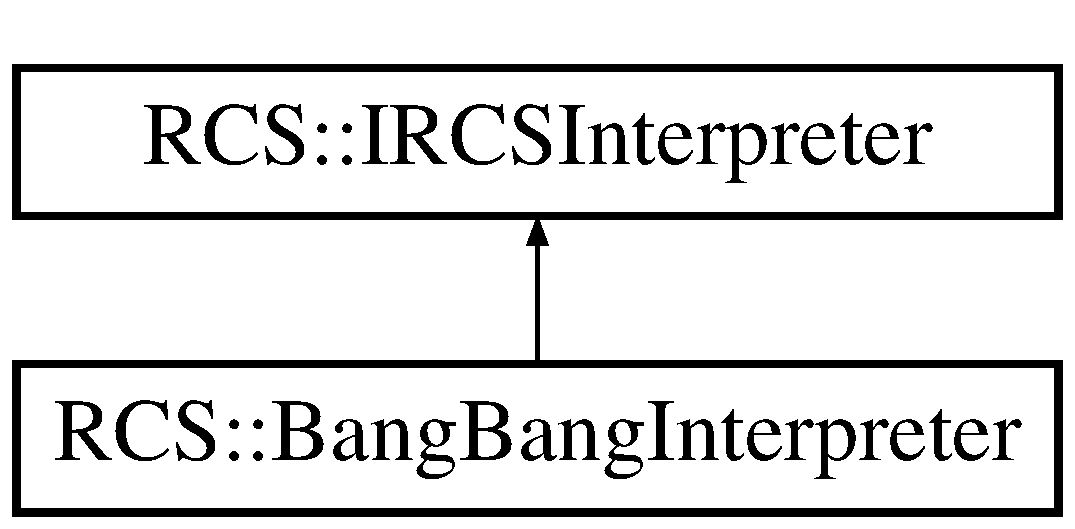
\includegraphics[height=2.000000cm]{classRCS_1_1IRCSInterpreter}
\end{center}
\end{figure}
\subsection*{Public Member Functions}
\begin{DoxyCompactItemize}
\item 
virtual \hyperlink{structRCS_1_1CanonCmd}{R\-C\-S\-::\-Canon\-Cmd} \hyperlink{classRCS_1_1IRCSInterpreter_adb4258abff48650cc30398ec996d04c1}{Parse\-Command} (\hyperlink{structRCS_1_1CanonCmd}{R\-C\-S\-::\-Canon\-Cmd} cmd)=0
\item 
virtual void \hyperlink{classRCS_1_1IRCSInterpreter_a5181a696aed581ae842bfd31537cfc1f}{Set\-Range} (std\-::vector$<$ double $>$ minrange, std\-::vector$<$ double $>$ maxrange)
\end{DoxyCompactItemize}


\subsection{Detailed Description}
I\-Interpreter parses a \hyperlink{namespaceRCS}{R\-C\-S} command and generates robot motion commands. 

\subsection{Member Function Documentation}
\hypertarget{classRCS_1_1IRCSInterpreter_adb4258abff48650cc30398ec996d04c1}{\index{R\-C\-S\-::\-I\-R\-C\-S\-Interpreter@{R\-C\-S\-::\-I\-R\-C\-S\-Interpreter}!Parse\-Command@{Parse\-Command}}
\index{Parse\-Command@{Parse\-Command}!RCS::IRCSInterpreter@{R\-C\-S\-::\-I\-R\-C\-S\-Interpreter}}
\subsubsection[{Parse\-Command}]{\setlength{\rightskip}{0pt plus 5cm}virtual {\bf R\-C\-S\-::\-Canon\-Cmd} R\-C\-S\-::\-I\-R\-C\-S\-Interpreter\-::\-Parse\-Command (
\begin{DoxyParamCaption}
\item[{{\bf R\-C\-S\-::\-Canon\-Cmd}}]{cmd}
\end{DoxyParamCaption}
)\hspace{0.3cm}{\ttfamily [pure virtual]}}}\label{classRCS_1_1IRCSInterpreter_adb4258abff48650cc30398ec996d04c1}


Implemented in \hyperlink{classRCS_1_1BangBangInterpreter_a7a5611f4e162defa15aeb1d503c7f3cb}{R\-C\-S\-::\-Bang\-Bang\-Interpreter}.

\hypertarget{classRCS_1_1IRCSInterpreter_a5181a696aed581ae842bfd31537cfc1f}{\index{R\-C\-S\-::\-I\-R\-C\-S\-Interpreter@{R\-C\-S\-::\-I\-R\-C\-S\-Interpreter}!Set\-Range@{Set\-Range}}
\index{Set\-Range@{Set\-Range}!RCS::IRCSInterpreter@{R\-C\-S\-::\-I\-R\-C\-S\-Interpreter}}
\subsubsection[{Set\-Range}]{\setlength{\rightskip}{0pt plus 5cm}virtual void R\-C\-S\-::\-I\-R\-C\-S\-Interpreter\-::\-Set\-Range (
\begin{DoxyParamCaption}
\item[{std\-::vector$<$ double $>$}]{minrange, }
\item[{std\-::vector$<$ double $>$}]{maxrange}
\end{DoxyParamCaption}
)\hspace{0.3cm}{\ttfamily [inline]}, {\ttfamily [virtual]}}}\label{classRCS_1_1IRCSInterpreter_a5181a696aed581ae842bfd31537cfc1f}


Reimplemented in \hyperlink{classRCS_1_1BangBangInterpreter_a69cc779236827f55ff895019e4833209}{R\-C\-S\-::\-Bang\-Bang\-Interpreter}.



The documentation for this class was generated from the following file\-:\begin{DoxyCompactItemize}
\item 
/usr/local/michalos/nistfanuc\-\_\-ws/src/nist\-\_\-fanuc/include/nist\-\_\-fanuc/\hyperlink{RCS_8h}{R\-C\-S.\-h}\end{DoxyCompactItemize}

\hypertarget{classKinematics}{\section{Kinematics Class Reference}
\label{classKinematics}\index{Kinematics@{Kinematics}}
}


{\ttfamily \#include $<$arm\-\_\-kinematics.\-h$>$}

\subsection*{Public Member Functions}
\begin{DoxyCompactItemize}
\item 
\hyperlink{classKinematics_af4e587252019eaa863b4246026296d4a}{Kinematics} ()
\item 
bool \hyperlink{classKinematics_adb7f126d671ba5fd9b07e999bc31c6b6}{init} (ros\-::\-Node\-Handle \&nh, std\-::string tipname, std\-::string rootname)
\item 
bool \hyperlink{classKinematics_a7dd98191224874c90c61870afe626557}{get\-Position\-I\-K} (moveit\-\_\-msgs\-::\-Get\-Position\-I\-K\-::\-Request \&request, moveit\-\_\-msgs\-::\-Get\-Position\-I\-K\-::\-Response \&response)
\begin{DoxyCompactList}\small\item\em This is the basic I\-K service method that will compute and return an I\-K solution. \end{DoxyCompactList}\item 
bool \hyperlink{classKinematics_a98e971f7084d97de2747d8ab4c337a14}{get\-I\-K\-Solver\-Info} (moveit\-\_\-msgs\-::\-Get\-Kinematic\-Solver\-Info\-::\-Request \&request, moveit\-\_\-msgs\-::\-Get\-Kinematic\-Solver\-Info\-::\-Response \&response)
\begin{DoxyCompactList}\small\item\em This is the basic kinematics info service that will return information about the kinematics node. \end{DoxyCompactList}\item 
bool \hyperlink{classKinematics_a2901a1b230c4b0cc59c8099c8bf485bd}{get\-F\-K\-Solver\-Info} (moveit\-\_\-msgs\-::\-Get\-Kinematic\-Solver\-Info\-::\-Request \&request, moveit\-\_\-msgs\-::\-Get\-Kinematic\-Solver\-Info\-::\-Response \&response)
\begin{DoxyCompactList}\small\item\em This is the basic kinematics info service that will return information about the kinematics node. \end{DoxyCompactList}\item 
bool \hyperlink{classKinematics_af444e591ca2efd584aee96d494ae8017}{get\-Position\-F\-K} (moveit\-\_\-msgs\-::\-Get\-Position\-F\-K\-::\-Request \&request, moveit\-\_\-msgs\-::\-Get\-Position\-F\-K\-::\-Response \&response)
\begin{DoxyCompactList}\small\item\em This is the basic forward kinematics service that will return information about the kinematics node. \end{DoxyCompactList}\end{DoxyCompactItemize}
\subsection*{Public Attributes}
\begin{DoxyCompactItemize}
\item 
K\-D\-L\-::\-Jnt\-Array \hyperlink{classKinematics_a2eb40bf5888be13788ac405d2b374fa9}{joint\-\_\-min}
\item 
K\-D\-L\-::\-Jnt\-Array \hyperlink{classKinematics_ac29342d180f646921535c4026e78862b}{joint\-\_\-max}
\item 
urdf\-::\-Model \hyperlink{classKinematics_a34e85bb69cc06af84aec250e03c8dce0}{robot\-\_\-model}
\end{DoxyCompactItemize}


\subsection{Constructor \& Destructor Documentation}
\hypertarget{classKinematics_af4e587252019eaa863b4246026296d4a}{\index{Kinematics@{Kinematics}!Kinematics@{Kinematics}}
\index{Kinematics@{Kinematics}!Kinematics@{Kinematics}}
\subsubsection[{Kinematics}]{\setlength{\rightskip}{0pt plus 5cm}Kinematics\-::\-Kinematics (
\begin{DoxyParamCaption}
{}
\end{DoxyParamCaption}
)}}\label{classKinematics_af4e587252019eaa863b4246026296d4a}


\subsection{Member Function Documentation}
\hypertarget{classKinematics_a2901a1b230c4b0cc59c8099c8bf485bd}{\index{Kinematics@{Kinematics}!get\-F\-K\-Solver\-Info@{get\-F\-K\-Solver\-Info}}
\index{get\-F\-K\-Solver\-Info@{get\-F\-K\-Solver\-Info}!Kinematics@{Kinematics}}
\subsubsection[{get\-F\-K\-Solver\-Info}]{\setlength{\rightskip}{0pt plus 5cm}bool Kinematics\-::get\-F\-K\-Solver\-Info (
\begin{DoxyParamCaption}
\item[{moveit\-\_\-msgs\-::\-Get\-Kinematic\-Solver\-Info\-::\-Request \&}]{request, }
\item[{moveit\-\_\-msgs\-::\-Get\-Kinematic\-Solver\-Info\-::\-Response \&}]{response}
\end{DoxyParamCaption}
)}}\label{classKinematics_a2901a1b230c4b0cc59c8099c8bf485bd}


This is the basic kinematics info service that will return information about the kinematics node. 


\begin{DoxyParams}{Parameters}
{\em A} & request message. See service definition for Get\-Kinematic\-Solver\-Info for more information on this message. \\
\hline
{\em The} & response message. See service definition for Get\-Kinematic\-Solver\-Info for more information on this message. \\
\hline
\end{DoxyParams}
\hypertarget{classKinematics_a98e971f7084d97de2747d8ab4c337a14}{\index{Kinematics@{Kinematics}!get\-I\-K\-Solver\-Info@{get\-I\-K\-Solver\-Info}}
\index{get\-I\-K\-Solver\-Info@{get\-I\-K\-Solver\-Info}!Kinematics@{Kinematics}}
\subsubsection[{get\-I\-K\-Solver\-Info}]{\setlength{\rightskip}{0pt plus 5cm}bool Kinematics\-::get\-I\-K\-Solver\-Info (
\begin{DoxyParamCaption}
\item[{moveit\-\_\-msgs\-::\-Get\-Kinematic\-Solver\-Info\-::\-Request \&}]{request, }
\item[{moveit\-\_\-msgs\-::\-Get\-Kinematic\-Solver\-Info\-::\-Response \&}]{response}
\end{DoxyParamCaption}
)}}\label{classKinematics_a98e971f7084d97de2747d8ab4c337a14}


This is the basic kinematics info service that will return information about the kinematics node. 


\begin{DoxyParams}{Parameters}
{\em A} & request message. See service definition for Get\-Kinematic\-Solver\-Info for more information on this message. \\
\hline
{\em The} & response message. See service definition for Get\-Kinematic\-Solver\-Info for more information on this message. \\
\hline
\end{DoxyParams}
\hypertarget{classKinematics_af444e591ca2efd584aee96d494ae8017}{\index{Kinematics@{Kinematics}!get\-Position\-F\-K@{get\-Position\-F\-K}}
\index{get\-Position\-F\-K@{get\-Position\-F\-K}!Kinematics@{Kinematics}}
\subsubsection[{get\-Position\-F\-K}]{\setlength{\rightskip}{0pt plus 5cm}bool Kinematics\-::get\-Position\-F\-K (
\begin{DoxyParamCaption}
\item[{moveit\-\_\-msgs\-::\-Get\-Position\-F\-K\-::\-Request \&}]{request, }
\item[{moveit\-\_\-msgs\-::\-Get\-Position\-F\-K\-::\-Response \&}]{response}
\end{DoxyParamCaption}
)}}\label{classKinematics_af444e591ca2efd584aee96d494ae8017}


This is the basic forward kinematics service that will return information about the kinematics node. 


\begin{DoxyParams}{Parameters}
{\em A} & request message. See service definition for Get\-Position\-F\-K for more information on this message. \\
\hline
{\em The} & response message. See service definition for Get\-Position\-F\-K for more information on this message. \\
\hline
\end{DoxyParams}
\hypertarget{classKinematics_a7dd98191224874c90c61870afe626557}{\index{Kinematics@{Kinematics}!get\-Position\-I\-K@{get\-Position\-I\-K}}
\index{get\-Position\-I\-K@{get\-Position\-I\-K}!Kinematics@{Kinematics}}
\subsubsection[{get\-Position\-I\-K}]{\setlength{\rightskip}{0pt plus 5cm}bool Kinematics\-::get\-Position\-I\-K (
\begin{DoxyParamCaption}
\item[{moveit\-\_\-msgs\-::\-Get\-Position\-I\-K\-::\-Request \&}]{request, }
\item[{moveit\-\_\-msgs\-::\-Get\-Position\-I\-K\-::\-Response \&}]{response}
\end{DoxyParamCaption}
)}}\label{classKinematics_a7dd98191224874c90c61870afe626557}


This is the basic I\-K service method that will compute and return an I\-K solution. 


\begin{DoxyParams}{Parameters}
{\em A} & request message. See service definition for Get\-Position\-I\-K for more information on this message. \\
\hline
{\em The} & response message. See service definition for Get\-Position\-I\-K for more information on this message. \\
\hline
\end{DoxyParams}
\hypertarget{classKinematics_adb7f126d671ba5fd9b07e999bc31c6b6}{\index{Kinematics@{Kinematics}!init@{init}}
\index{init@{init}!Kinematics@{Kinematics}}
\subsubsection[{init}]{\setlength{\rightskip}{0pt plus 5cm}bool Kinematics\-::init (
\begin{DoxyParamCaption}
\item[{ros\-::\-Node\-Handle \&}]{nh, }
\item[{std\-::string}]{tipname, }
\item[{std\-::string}]{rootname}
\end{DoxyParamCaption}
)}}\label{classKinematics_adb7f126d671ba5fd9b07e999bc31c6b6}


\subsection{Member Data Documentation}
\hypertarget{classKinematics_ac29342d180f646921535c4026e78862b}{\index{Kinematics@{Kinematics}!joint\-\_\-max@{joint\-\_\-max}}
\index{joint\-\_\-max@{joint\-\_\-max}!Kinematics@{Kinematics}}
\subsubsection[{joint\-\_\-max}]{\setlength{\rightskip}{0pt plus 5cm}K\-D\-L\-::\-Jnt\-Array Kinematics\-::joint\-\_\-max}}\label{classKinematics_ac29342d180f646921535c4026e78862b}
\hypertarget{classKinematics_a2eb40bf5888be13788ac405d2b374fa9}{\index{Kinematics@{Kinematics}!joint\-\_\-min@{joint\-\_\-min}}
\index{joint\-\_\-min@{joint\-\_\-min}!Kinematics@{Kinematics}}
\subsubsection[{joint\-\_\-min}]{\setlength{\rightskip}{0pt plus 5cm}K\-D\-L\-::\-Jnt\-Array Kinematics\-::joint\-\_\-min}}\label{classKinematics_a2eb40bf5888be13788ac405d2b374fa9}
\hypertarget{classKinematics_a34e85bb69cc06af84aec250e03c8dce0}{\index{Kinematics@{Kinematics}!robot\-\_\-model@{robot\-\_\-model}}
\index{robot\-\_\-model@{robot\-\_\-model}!Kinematics@{Kinematics}}
\subsubsection[{robot\-\_\-model}]{\setlength{\rightskip}{0pt plus 5cm}urdf\-::\-Model Kinematics\-::robot\-\_\-model}}\label{classKinematics_a34e85bb69cc06af84aec250e03c8dce0}


The documentation for this class was generated from the following files\-:\begin{DoxyCompactItemize}
\item 
/usr/local/michalos/nistfanuc\-\_\-ws/src/nist\-\_\-fanuc/include/nist\-\_\-fanuc/\hyperlink{arm__kinematics_8h}{arm\-\_\-kinematics.\-h}\item 
/usr/local/michalos/nistfanuc\-\_\-ws/src/nist\-\_\-fanuc/src/\hyperlink{arm__kinematics_8cpp}{arm\-\_\-kinematics.\-cpp}\end{DoxyCompactItemize}

\hypertarget{classMotionControl}{\section{Motion\-Control Class Reference}
\label{classMotionControl}\index{Motion\-Control@{Motion\-Control}}
}


\hyperlink{classMotionControl}{Motion\-Control} is a class that contains some useful motion control methods.  




{\ttfamily \#include $<$Motion\-Control.\-h$>$}

\subsection*{Public Member Functions}
\begin{DoxyCompactItemize}
\item 
bool \hyperlink{classMotionControl_a7d4bdb16c10626850dac271d30428f71}{execute\-Trajectory} (const trajectory\-\_\-msgs\-::\-Joint\-Trajectory \&trajectory, const std\-::string \&trajectory\-\_\-ns)
\begin{DoxyCompactList}\small\item\em execute\-Trajectory will send a traject to ros to execute \end{DoxyCompactList}\item 
\hyperlink{namespaceRCS_aa07e45d8a50e30064283d2b38087f999}{R\-C\-S\-::\-Pose} \hyperlink{classMotionControl_a9d242a51b301d7c87c16f579e0d9347e}{compute\-Translation} (\hyperlink{namespaceRCS_aa07e45d8a50e30064283d2b38087f999}{R\-C\-S\-::\-Pose} \&\-\_\-cur\-Pos, \hyperlink{namespaceRCS_aa07e45d8a50e30064283d2b38087f999}{R\-C\-S\-::\-Pose} \&\-\_\-goal\-Pos, double d\-Increment)
\begin{DoxyCompactList}\small\item\em Return linear interpolation (lerp) between current and goal translation. \end{DoxyCompactList}\item 
std\-::vector$<$ \hyperlink{namespaceRCS_aa07e45d8a50e30064283d2b38087f999}{R\-C\-S\-::\-Pose} $>$ \hyperlink{classMotionControl_a40113f305b3accd4d28fa976151aa954}{compute\-Waypoints} (\hyperlink{namespaceRCS_aa07e45d8a50e30064283d2b38087f999}{R\-C\-S\-::\-Pose} \&\-\_\-cur\-Pos, \hyperlink{namespaceRCS_aa07e45d8a50e30064283d2b38087f999}{R\-C\-S\-::\-Pose} \&\-\_\-goal\-Pos, double d\-Gap=0.\-001, bool b\-Add\-Start=false)
\begin{DoxyCompactList}\small\item\em Compute waypoints between current and goal poses with assigned distance between poses. \end{DoxyCompactList}\item 
std\-::vector$<$ \hyperlink{RCS_8h_aa4adb93a26caa4dacba9c9614e283245}{Joint\-State} $>$ \hyperlink{classMotionControl_aebf1d77a70bbf6817f0899a98173b87d}{compute\-Coorindated\-Waypoints} (std\-::vector$<$ double $>$ \&\-\_\-cur\-Jts, std\-::vector$<$ double $>$ \&\-\_\-goal\-Jts, double d\-Gap=0.\-001, bool b\-Add\-Start=false)
\begin{DoxyCompactList}\small\item\em compute\-Coorindated\-Waypoints returns a vector of straightline waypoints between current and goal poses at a given distance. Joints arrive a destination at the same time within the trajectory. \end{DoxyCompactList}\item 
std\-::vector$<$ \hyperlink{RCS_8h_aa4adb93a26caa4dacba9c9614e283245}{Joint\-State} $>$ \hyperlink{classMotionControl_a5a7f01d81030676aab106b7bf4c60aa6}{compute\-Uncoorindated\-Waypoints} (std\-::vector$<$ double $>$ \&\-\_\-cur\-Jts, std\-::vector$<$ double $>$ \&\-\_\-goal\-Jts, double d\-Gap=0.\-001, bool b\-Add\-Start=false)
\begin{DoxyCompactList}\small\item\em compute\-Uncoorindated\-Waypoints returns a vector of waypoints between current and goal poses at a given distance. Joints arrive a destination at various times in the trajectory. \end{DoxyCompactList}\item 
int \hyperlink{classMotionControl_ac065f800e86df7a771aae2aa4271aaa3}{compute\-Increments} (std\-::vector$<$ double $>$ \&\-\_\-cur\-Jts, std\-::vector$<$ double $>$ \&\-\_\-goal\-Jts, double gap=0.\-001)
\item 
int \hyperlink{classMotionControl_a1dbb240abf15324af65904bfba39bd41}{compute\-Increments} (\hyperlink{namespaceRCS_aa07e45d8a50e30064283d2b38087f999}{R\-C\-S\-::\-Pose} \&\-\_\-cur\-Pos, \hyperlink{namespaceRCS_aa07e45d8a50e30064283d2b38087f999}{R\-C\-S\-::\-Pose} \&\-\_\-goal\-Pos, double d\-Gap=0.\-001)
\end{DoxyCompactItemize}
\subsection*{Static Public Member Functions}
\begin{DoxyCompactItemize}
\item 
static bool \hyperlink{classMotionControl_a57fb4b492bc50f10b4fd5e068bda4f7a}{At\-Goal} (\hyperlink{RCS_8h_aa4adb93a26caa4dacba9c9614e283245}{Joint\-State} goal, \hyperlink{RCS_8h_aa4adb93a26caa4dacba9c9614e283245}{Joint\-State} current, double \hyperlink{classMotionControl_ad3cadb7d245794540e4a320ee560b6b2}{epsilon}=0.\-001)
\begin{DoxyCompactList}\small\item\em At\-Goal will determine if a pair joint state values are equal (within an epsilon tolerance). \end{DoxyCompactList}\end{DoxyCompactItemize}
\subsection*{Static Public Attributes}
\begin{DoxyCompactItemize}
\item 
static double \hyperlink{classMotionControl_ad3cadb7d245794540e4a320ee560b6b2}{epsilon} = 0.\-001
\end{DoxyCompactItemize}


\subsection{Detailed Description}
\hyperlink{classMotionControl}{Motion\-Control} is a class that contains some useful motion control methods. 

\subsection{Member Function Documentation}
\hypertarget{classMotionControl_a57fb4b492bc50f10b4fd5e068bda4f7a}{\index{Motion\-Control@{Motion\-Control}!At\-Goal@{At\-Goal}}
\index{At\-Goal@{At\-Goal}!MotionControl@{Motion\-Control}}
\subsubsection[{At\-Goal}]{\setlength{\rightskip}{0pt plus 5cm}bool Motion\-Control\-::\-At\-Goal (
\begin{DoxyParamCaption}
\item[{{\bf Joint\-State}}]{goal, }
\item[{{\bf Joint\-State}}]{current, }
\item[{double}]{epsilon = {\ttfamily 0.001}}
\end{DoxyParamCaption}
)\hspace{0.3cm}{\ttfamily [static]}}}\label{classMotionControl_a57fb4b492bc50f10b4fd5e068bda4f7a}


At\-Goal will determine if a pair joint state values are equal (within an epsilon tolerance). 


\begin{DoxyParams}{Parameters}
{\em goal} & description of goal joint state \\
\hline
{\em current} & description of current joint state \\
\hline
{\em epsilon} & tolerance of equality \\
\hline
\end{DoxyParams}
\begin{DoxyReturn}{Returns}
boolean whether robot is at the desired goal described in joint values. 
\end{DoxyReturn}
\hypertarget{classMotionControl_aebf1d77a70bbf6817f0899a98173b87d}{\index{Motion\-Control@{Motion\-Control}!compute\-Coorindated\-Waypoints@{compute\-Coorindated\-Waypoints}}
\index{compute\-Coorindated\-Waypoints@{compute\-Coorindated\-Waypoints}!MotionControl@{Motion\-Control}}
\subsubsection[{compute\-Coorindated\-Waypoints}]{\setlength{\rightskip}{0pt plus 5cm}std\-::vector$<$ {\bf Joint\-State} $>$ Motion\-Control\-::compute\-Coorindated\-Waypoints (
\begin{DoxyParamCaption}
\item[{std\-::vector$<$ double $>$ \&}]{\-\_\-cur\-Jts, }
\item[{std\-::vector$<$ double $>$ \&}]{\-\_\-goal\-Jts, }
\item[{double}]{d\-Gap = {\ttfamily 0.001}, }
\item[{bool}]{b\-Add\-Start = {\ttfamily false}}
\end{DoxyParamCaption}
)}}\label{classMotionControl_aebf1d77a70bbf6817f0899a98173b87d}


compute\-Coorindated\-Waypoints returns a vector of straightline waypoints between current and goal poses at a given distance. Joints arrive a destination at the same time within the trajectory. 


\begin{DoxyParams}{Parameters}
{\em \-\_\-cur\-Pos} & description of current pose \\
\hline
{\em \-\_\-goal\-Pos} & description of goal pose \\
\hline
{\em gap} & distance between waypoints \\
\hline
{\em b\-Add\-Start} & boolean to determine if starting pose is included in waypoints \\
\hline
\end{DoxyParams}
\begin{DoxyReturn}{Returns}
vector of straighline waypoint poses with gap distance between poses. 
\end{DoxyReturn}
\hypertarget{classMotionControl_ac065f800e86df7a771aae2aa4271aaa3}{\index{Motion\-Control@{Motion\-Control}!compute\-Increments@{compute\-Increments}}
\index{compute\-Increments@{compute\-Increments}!MotionControl@{Motion\-Control}}
\subsubsection[{compute\-Increments}]{\setlength{\rightskip}{0pt plus 5cm}int Motion\-Control\-::compute\-Increments (
\begin{DoxyParamCaption}
\item[{std\-::vector$<$ double $>$ \&}]{\-\_\-cur\-Jts, }
\item[{std\-::vector$<$ double $>$ \&}]{\-\_\-goal\-Jts, }
\item[{double}]{gap = {\ttfamily 0.001}}
\end{DoxyParamCaption}
)}}\label{classMotionControl_ac065f800e86df7a771aae2aa4271aaa3}
\hypertarget{classMotionControl_a1dbb240abf15324af65904bfba39bd41}{\index{Motion\-Control@{Motion\-Control}!compute\-Increments@{compute\-Increments}}
\index{compute\-Increments@{compute\-Increments}!MotionControl@{Motion\-Control}}
\subsubsection[{compute\-Increments}]{\setlength{\rightskip}{0pt plus 5cm}int Motion\-Control\-::compute\-Increments (
\begin{DoxyParamCaption}
\item[{{\bf R\-C\-S\-::\-Pose} \&}]{\-\_\-cur\-Pos, }
\item[{{\bf R\-C\-S\-::\-Pose} \&}]{\-\_\-goal\-Pos, }
\item[{double}]{d\-Gap = {\ttfamily 0.001}}
\end{DoxyParamCaption}
)}}\label{classMotionControl_a1dbb240abf15324af65904bfba39bd41}
\hypertarget{classMotionControl_a9d242a51b301d7c87c16f579e0d9347e}{\index{Motion\-Control@{Motion\-Control}!compute\-Translation@{compute\-Translation}}
\index{compute\-Translation@{compute\-Translation}!MotionControl@{Motion\-Control}}
\subsubsection[{compute\-Translation}]{\setlength{\rightskip}{0pt plus 5cm}{\bf R\-C\-S\-::\-Pose} Motion\-Control\-::compute\-Translation (
\begin{DoxyParamCaption}
\item[{{\bf R\-C\-S\-::\-Pose} \&}]{\-\_\-cur\-Pos, }
\item[{{\bf R\-C\-S\-::\-Pose} \&}]{\-\_\-goal\-Pos, }
\item[{double}]{d\-Increment}
\end{DoxyParamCaption}
)}}\label{classMotionControl_a9d242a51b301d7c87c16f579e0d9347e}


Return linear interpolation (lerp) between current and goal translation. 


\begin{DoxyParams}{Parameters}
{\em \-\_\-cur\-Pos} & description of current pose \\
\hline
{\em \-\_\-goal\-Pos} & description of goal pose \\
\hline
{\em d\-Increment} & translation amount from \mbox{[}0..1\mbox{]} \\
\hline
\end{DoxyParams}
\begin{DoxyReturn}{Returns}
pose containing lerped pose translation. 
\end{DoxyReturn}
\hypertarget{classMotionControl_a5a7f01d81030676aab106b7bf4c60aa6}{\index{Motion\-Control@{Motion\-Control}!compute\-Uncoorindated\-Waypoints@{compute\-Uncoorindated\-Waypoints}}
\index{compute\-Uncoorindated\-Waypoints@{compute\-Uncoorindated\-Waypoints}!MotionControl@{Motion\-Control}}
\subsubsection[{compute\-Uncoorindated\-Waypoints}]{\setlength{\rightskip}{0pt plus 5cm}std\-::vector$<$ {\bf Joint\-State} $>$ Motion\-Control\-::compute\-Uncoorindated\-Waypoints (
\begin{DoxyParamCaption}
\item[{std\-::vector$<$ double $>$ \&}]{\-\_\-cur\-Jts, }
\item[{std\-::vector$<$ double $>$ \&}]{\-\_\-goal\-Jts, }
\item[{double}]{d\-Gap = {\ttfamily 0.001}, }
\item[{bool}]{b\-Add\-Start = {\ttfamily false}}
\end{DoxyParamCaption}
)}}\label{classMotionControl_a5a7f01d81030676aab106b7bf4c60aa6}


compute\-Uncoorindated\-Waypoints returns a vector of waypoints between current and goal poses at a given distance. Joints arrive a destination at various times in the trajectory. 


\begin{DoxyParams}{Parameters}
{\em \-\_\-cur\-Pos} & description of current pose \\
\hline
{\em \-\_\-goal\-Pos} & description of goal pose \\
\hline
{\em gap} & distance between waypoints \\
\hline
{\em b\-Add\-Start} & boolean to determine if starting pose is included in waypoints \\
\hline
\end{DoxyParams}
\begin{DoxyReturn}{Returns}
vector of straighline waypoint poses with gap distance between poses. 
\end{DoxyReturn}
\hypertarget{classMotionControl_a40113f305b3accd4d28fa976151aa954}{\index{Motion\-Control@{Motion\-Control}!compute\-Waypoints@{compute\-Waypoints}}
\index{compute\-Waypoints@{compute\-Waypoints}!MotionControl@{Motion\-Control}}
\subsubsection[{compute\-Waypoints}]{\setlength{\rightskip}{0pt plus 5cm}std\-::vector$<$ {\bf R\-C\-S\-::\-Pose} $>$ Motion\-Control\-::compute\-Waypoints (
\begin{DoxyParamCaption}
\item[{{\bf R\-C\-S\-::\-Pose} \&}]{\-\_\-cur\-Pos, }
\item[{{\bf R\-C\-S\-::\-Pose} \&}]{\-\_\-goal\-Pos, }
\item[{double}]{d\-Gap = {\ttfamily 0.001}, }
\item[{bool}]{b\-Add\-Start = {\ttfamily false}}
\end{DoxyParamCaption}
)}}\label{classMotionControl_a40113f305b3accd4d28fa976151aa954}


Compute waypoints between current and goal poses with assigned distance between poses. 


\begin{DoxyParams}{Parameters}
{\em \-\_\-cur\-Pos} & description of current pose \\
\hline
{\em \-\_\-goal\-Pos} & description of goal pose \\
\hline
{\em gap} & distance between waypoints \\
\hline
{\em b\-Add\-Start} & boolean to determine if starting pose is included in waypoints \\
\hline
\end{DoxyParams}
\begin{DoxyReturn}{Returns}
vector of waypoint poses with gap distance between poses. 
\end{DoxyReturn}
\hypertarget{classMotionControl_a7d4bdb16c10626850dac271d30428f71}{\index{Motion\-Control@{Motion\-Control}!execute\-Trajectory@{execute\-Trajectory}}
\index{execute\-Trajectory@{execute\-Trajectory}!MotionControl@{Motion\-Control}}
\subsubsection[{execute\-Trajectory}]{\setlength{\rightskip}{0pt plus 5cm}bool Motion\-Control\-::execute\-Trajectory (
\begin{DoxyParamCaption}
\item[{const trajectory\-\_\-msgs\-::\-Joint\-Trajectory \&}]{trajectory, }
\item[{const std\-::string \&}]{trajectory\-\_\-ns}
\end{DoxyParamCaption}
)}}\label{classMotionControl_a7d4bdb16c10626850dac271d30428f71}


execute\-Trajectory will send a traject to ros to execute 


\begin{DoxyParams}{Parameters}
{\em trajectory} & \\
\hline
{\em trajectory\-\_\-ns} & namespace of trajectory \\
\hline
\end{DoxyParams}
\begin{DoxyReturn}{Returns}
boolean whether success or failure 
\end{DoxyReturn}


\subsection{Member Data Documentation}
\hypertarget{classMotionControl_ad3cadb7d245794540e4a320ee560b6b2}{\index{Motion\-Control@{Motion\-Control}!epsilon@{epsilon}}
\index{epsilon@{epsilon}!MotionControl@{Motion\-Control}}
\subsubsection[{epsilon}]{\setlength{\rightskip}{0pt plus 5cm}double Motion\-Control\-::epsilon = 0.\-001\hspace{0.3cm}{\ttfamily [static]}}}\label{classMotionControl_ad3cadb7d245794540e4a320ee560b6b2}
allowable difference length in equality between two numbers 

The documentation for this class was generated from the following files\-:\begin{DoxyCompactItemize}
\item 
/usr/local/michalos/github/usnistgov/el-\/robotics-\/core/nist\-\_\-fanuc/include/nist\-\_\-fanuc/\hyperlink{MotionControl_8h}{Motion\-Control.\-h}\item 
/usr/local/michalos/github/usnistgov/el-\/robotics-\/core/nist\-\_\-fanuc/src/\hyperlink{MotionControl_8cpp}{Motion\-Control.\-cpp}\end{DoxyCompactItemize}

\hypertarget{classMotomanNearestJointsLookup}{\section{Motoman\-Nearest\-Joints\-Lookup Class Reference}
\label{classMotomanNearestJointsLookup}\index{Motoman\-Nearest\-Joints\-Lookup@{Motoman\-Nearest\-Joints\-Lookup}}
}


{\ttfamily \#include $<$Demo.\-h$>$}

Inheritance diagram for Motoman\-Nearest\-Joints\-Lookup\-:\begin{figure}[H]
\begin{center}
\leavevmode
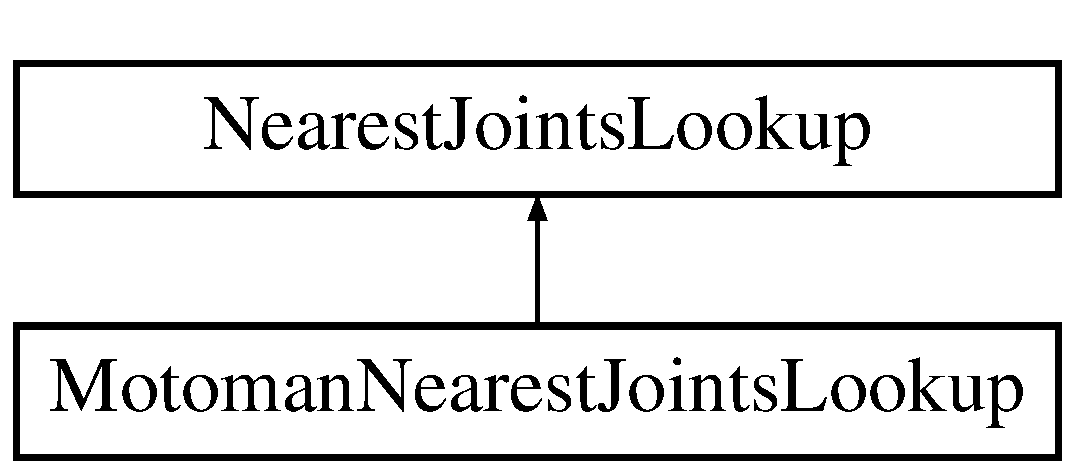
\includegraphics[height=2.000000cm]{classMotomanNearestJointsLookup}
\end{center}
\end{figure}
\subsection*{Public Member Functions}
\begin{DoxyCompactItemize}
\item 
\hyperlink{classMotomanNearestJointsLookup_a98735da0485f02fb789297aefbe3c367}{Motoman\-Nearest\-Joints\-Lookup} (tf\-::\-Pose baseoffset, \hyperlink{Kinematics_8h_aa720b9842c846588baf215581fb9f902}{I\-Kinematics\-Shared\-Ptr} kin)
\item 
virtual void \hyperlink{classMotomanNearestJointsLookup_a4eb36439bed74cecca93decece53d9ff}{Set\-Robot\-Hints} ()
\begin{DoxyCompactList}\small\item\em Either ik or more trajectory control with spacing between joint updates small so K\-D\-L happy. \end{DoxyCompactList}\end{DoxyCompactItemize}
\subsection*{Additional Inherited Members}


\subsection{Constructor \& Destructor Documentation}
\hypertarget{classMotomanNearestJointsLookup_a98735da0485f02fb789297aefbe3c367}{\index{Motoman\-Nearest\-Joints\-Lookup@{Motoman\-Nearest\-Joints\-Lookup}!Motoman\-Nearest\-Joints\-Lookup@{Motoman\-Nearest\-Joints\-Lookup}}
\index{Motoman\-Nearest\-Joints\-Lookup@{Motoman\-Nearest\-Joints\-Lookup}!MotomanNearestJointsLookup@{Motoman\-Nearest\-Joints\-Lookup}}
\subsubsection[{Motoman\-Nearest\-Joints\-Lookup}]{\setlength{\rightskip}{0pt plus 5cm}Motoman\-Nearest\-Joints\-Lookup\-::\-Motoman\-Nearest\-Joints\-Lookup (
\begin{DoxyParamCaption}
\item[{tf\-::\-Pose}]{baseoffset, }
\item[{{\bf I\-Kinematics\-Shared\-Ptr}}]{kin}
\end{DoxyParamCaption}
)\hspace{0.3cm}{\ttfamily [inline]}}}\label{classMotomanNearestJointsLookup_a98735da0485f02fb789297aefbe3c367}


\subsection{Member Function Documentation}
\hypertarget{classMotomanNearestJointsLookup_a4eb36439bed74cecca93decece53d9ff}{\index{Motoman\-Nearest\-Joints\-Lookup@{Motoman\-Nearest\-Joints\-Lookup}!Set\-Robot\-Hints@{Set\-Robot\-Hints}}
\index{Set\-Robot\-Hints@{Set\-Robot\-Hints}!MotomanNearestJointsLookup@{Motoman\-Nearest\-Joints\-Lookup}}
\subsubsection[{Set\-Robot\-Hints}]{\setlength{\rightskip}{0pt plus 5cm}void Motoman\-Nearest\-Joints\-Lookup\-::\-Set\-Robot\-Hints (
\begin{DoxyParamCaption}
{}
\end{DoxyParamCaption}
)\hspace{0.3cm}{\ttfamily [virtual]}}}\label{classMotomanNearestJointsLookup_a4eb36439bed74cecca93decece53d9ff}


Either ik or more trajectory control with spacing between joint updates small so K\-D\-L happy. 



Reimplemented from \hyperlink{classNearestJointsLookup_a833cff3f82b12344d2142690e6216340}{Nearest\-Joints\-Lookup}.



The documentation for this class was generated from the following files\-:\begin{DoxyCompactItemize}
\item 
/usr/local/michalos/nistfanuc\-\_\-ws/src/nist\-\_\-fanuc/include/nist\-\_\-fanuc/\hyperlink{Demo_8h}{Demo.\-h}\item 
/usr/local/michalos/nistfanuc\-\_\-ws/src/nist\-\_\-fanuc/src/\hyperlink{Demo_8cpp}{Demo.\-cpp}\end{DoxyCompactItemize}

\hypertarget{structCheckers_1_1Move}{\section{Checkers\-:\-:Move Struct Reference}
\label{structCheckers_1_1Move}\index{Checkers\-::\-Move@{Checkers\-::\-Move}}
}


{\ttfamily \#include $<$Checkers.\-h$>$}

\subsection*{Public Member Functions}
\begin{DoxyCompactItemize}
\item 
\hyperlink{structCheckers_1_1Move_a60f00f24995512613aa98275bec58210}{Move} ()
\item 
\hyperlink{structCheckers_1_1Move_a8515cd0b6a9455950e811df92bceb090}{Move} (int \hyperlink{structCheckers_1_1Move_a2f318313b9288decf1144fcc8da4457f}{row}, int \hyperlink{structCheckers_1_1Move_ac78fddc38b24f19fe07c5cd61be59fb9}{col}, bool \hyperlink{structCheckers_1_1Move_a037e2f59611b937d8517454e98df3311}{b\-Jump}=false)
\item 
void \hyperlink{structCheckers_1_1Move_a0c905df569d2a84b74a23799e286d6c3}{Start} (int \hyperlink{structCheckers_1_1Move_a45735e4fab8cae7dc01f8ec8eba86679}{player}, int \hyperlink{structCheckers_1_1Move_a2f318313b9288decf1144fcc8da4457f}{row}, int \hyperlink{structCheckers_1_1Move_ac78fddc38b24f19fe07c5cd61be59fb9}{col})
\item 
\hyperlink{structCheckers_1_1Move}{Move} \hyperlink{structCheckers_1_1Move_ae52bcf1d81c9f69ddb4f3d300bdb2a2f}{Diff} (\hyperlink{structCheckers_1_1Move}{Move} start)
\end{DoxyCompactItemize}
\subsection*{Public Attributes}
\begin{DoxyCompactItemize}
\item 
int \hyperlink{structCheckers_1_1Move_a2f318313b9288decf1144fcc8da4457f}{row}
\item 
int \hyperlink{structCheckers_1_1Move_ac78fddc38b24f19fe07c5cd61be59fb9}{col}
\item 
int \hyperlink{structCheckers_1_1Move_a45735e4fab8cae7dc01f8ec8eba86679}{player}
\item 
bool \hyperlink{structCheckers_1_1Move_a037e2f59611b937d8517454e98df3311}{b\-Jump}
\item 
bool \hyperlink{structCheckers_1_1Move_a5626549bbd2a7d53ffe3ab183790a6c5}{b\-Double\-Jumps}
\item 
std\-::vector$<$ \hyperlink{structCheckers_1_1Move}{Move} $>$ \hyperlink{structCheckers_1_1Move_abc9f00e18c240b745872cbaf57f265fa}{doublejumps}
\item 
int \hyperlink{structCheckers_1_1Move_a3cf599693d1ee27b69d49fb60b55db0a}{srow}
\item 
int \hyperlink{structCheckers_1_1Move_a8bb137b74b8fef49def2fed2ad19d7ef}{scol}
\item 
double \hyperlink{structCheckers_1_1Move_a2fbd62e73c5906404f0153a17385a25f}{score}
\end{DoxyCompactItemize}
\subsection*{Friends}
\begin{DoxyCompactItemize}
\item 
bool \hyperlink{structCheckers_1_1Move_a91c817929e7d1a0fd029b500194c88bd}{operator$<$} (const \hyperlink{structCheckers_1_1Move}{Move} \&left, const \hyperlink{structCheckers_1_1Move}{Move} \&other)
\item 
std\-::ostream \& \hyperlink{structCheckers_1_1Move_a046ca51bde34e23abd6ca6597d16025d}{operator$<$$<$} (std\-::ostream \&output\-\_\-out, const \hyperlink{structCheckers_1_1Move}{Move} \&move\-\_\-in)
\item 
std\-::istream \& \hyperlink{structCheckers_1_1Move_a07dcbb6b5ce4d1ba0cc4b9d60cce563c}{operator$>$$>$} (std\-::istream \&s\-\_\-in, \hyperlink{structCheckers_1_1Move}{Move} \&move\-\_\-out)
\end{DoxyCompactItemize}


\subsection{Constructor \& Destructor Documentation}
\hypertarget{structCheckers_1_1Move_a60f00f24995512613aa98275bec58210}{\index{Checkers\-::\-Move@{Checkers\-::\-Move}!Move@{Move}}
\index{Move@{Move}!Checkers::Move@{Checkers\-::\-Move}}
\subsubsection[{Move}]{\setlength{\rightskip}{0pt plus 5cm}Checkers\-::\-Move\-::\-Move (
\begin{DoxyParamCaption}
{}
\end{DoxyParamCaption}
)\hspace{0.3cm}{\ttfamily [inline]}}}\label{structCheckers_1_1Move_a60f00f24995512613aa98275bec58210}
\hypertarget{structCheckers_1_1Move_a8515cd0b6a9455950e811df92bceb090}{\index{Checkers\-::\-Move@{Checkers\-::\-Move}!Move@{Move}}
\index{Move@{Move}!Checkers::Move@{Checkers\-::\-Move}}
\subsubsection[{Move}]{\setlength{\rightskip}{0pt plus 5cm}Checkers\-::\-Move\-::\-Move (
\begin{DoxyParamCaption}
\item[{int}]{row, }
\item[{int}]{col, }
\item[{bool}]{b\-Jump = {\ttfamily false}}
\end{DoxyParamCaption}
)\hspace{0.3cm}{\ttfamily [inline]}}}\label{structCheckers_1_1Move_a8515cd0b6a9455950e811df92bceb090}


\subsection{Member Function Documentation}
\hypertarget{structCheckers_1_1Move_ae52bcf1d81c9f69ddb4f3d300bdb2a2f}{\index{Checkers\-::\-Move@{Checkers\-::\-Move}!Diff@{Diff}}
\index{Diff@{Diff}!Checkers::Move@{Checkers\-::\-Move}}
\subsubsection[{Diff}]{\setlength{\rightskip}{0pt plus 5cm}{\bf Move} Checkers\-::\-Move\-::\-Diff (
\begin{DoxyParamCaption}
\item[{{\bf Move}}]{start}
\end{DoxyParamCaption}
)\hspace{0.3cm}{\ttfamily [inline]}}}\label{structCheckers_1_1Move_ae52bcf1d81c9f69ddb4f3d300bdb2a2f}
\hypertarget{structCheckers_1_1Move_a0c905df569d2a84b74a23799e286d6c3}{\index{Checkers\-::\-Move@{Checkers\-::\-Move}!Start@{Start}}
\index{Start@{Start}!Checkers::Move@{Checkers\-::\-Move}}
\subsubsection[{Start}]{\setlength{\rightskip}{0pt plus 5cm}void Checkers\-::\-Move\-::\-Start (
\begin{DoxyParamCaption}
\item[{int}]{player, }
\item[{int}]{row, }
\item[{int}]{col}
\end{DoxyParamCaption}
)\hspace{0.3cm}{\ttfamily [inline]}}}\label{structCheckers_1_1Move_a0c905df569d2a84b74a23799e286d6c3}


\subsection{Friends And Related Function Documentation}
\hypertarget{structCheckers_1_1Move_a91c817929e7d1a0fd029b500194c88bd}{\index{Checkers\-::\-Move@{Checkers\-::\-Move}!operator$<$@{operator$<$}}
\index{operator$<$@{operator$<$}!Checkers::Move@{Checkers\-::\-Move}}
\subsubsection[{operator$<$}]{\setlength{\rightskip}{0pt plus 5cm}bool operator$<$ (
\begin{DoxyParamCaption}
\item[{const {\bf Move} \&}]{left, }
\item[{const {\bf Move} \&}]{other}
\end{DoxyParamCaption}
)\hspace{0.3cm}{\ttfamily [friend]}}}\label{structCheckers_1_1Move_a91c817929e7d1a0fd029b500194c88bd}
\hypertarget{structCheckers_1_1Move_a046ca51bde34e23abd6ca6597d16025d}{\index{Checkers\-::\-Move@{Checkers\-::\-Move}!operator$<$$<$@{operator$<$$<$}}
\index{operator$<$$<$@{operator$<$$<$}!Checkers::Move@{Checkers\-::\-Move}}
\subsubsection[{operator$<$$<$}]{\setlength{\rightskip}{0pt plus 5cm}std\-::ostream\& operator$<$$<$ (
\begin{DoxyParamCaption}
\item[{std\-::ostream \&}]{output\-\_\-out, }
\item[{const {\bf Move} \&}]{move\-\_\-in}
\end{DoxyParamCaption}
)\hspace{0.3cm}{\ttfamily [friend]}}}\label{structCheckers_1_1Move_a046ca51bde34e23abd6ca6597d16025d}
\hypertarget{structCheckers_1_1Move_a07dcbb6b5ce4d1ba0cc4b9d60cce563c}{\index{Checkers\-::\-Move@{Checkers\-::\-Move}!operator$>$$>$@{operator$>$$>$}}
\index{operator$>$$>$@{operator$>$$>$}!Checkers::Move@{Checkers\-::\-Move}}
\subsubsection[{operator$>$$>$}]{\setlength{\rightskip}{0pt plus 5cm}std\-::istream\& operator$>$$>$ (
\begin{DoxyParamCaption}
\item[{std\-::istream \&}]{s\-\_\-in, }
\item[{{\bf Move} \&}]{move\-\_\-out}
\end{DoxyParamCaption}
)\hspace{0.3cm}{\ttfamily [friend]}}}\label{structCheckers_1_1Move_a07dcbb6b5ce4d1ba0cc4b9d60cce563c}


\subsection{Member Data Documentation}
\hypertarget{structCheckers_1_1Move_a5626549bbd2a7d53ffe3ab183790a6c5}{\index{Checkers\-::\-Move@{Checkers\-::\-Move}!b\-Double\-Jumps@{b\-Double\-Jumps}}
\index{b\-Double\-Jumps@{b\-Double\-Jumps}!Checkers::Move@{Checkers\-::\-Move}}
\subsubsection[{b\-Double\-Jumps}]{\setlength{\rightskip}{0pt plus 5cm}bool Checkers\-::\-Move\-::b\-Double\-Jumps}}\label{structCheckers_1_1Move_a5626549bbd2a7d53ffe3ab183790a6c5}
\hypertarget{structCheckers_1_1Move_a037e2f59611b937d8517454e98df3311}{\index{Checkers\-::\-Move@{Checkers\-::\-Move}!b\-Jump@{b\-Jump}}
\index{b\-Jump@{b\-Jump}!Checkers::Move@{Checkers\-::\-Move}}
\subsubsection[{b\-Jump}]{\setlength{\rightskip}{0pt plus 5cm}bool Checkers\-::\-Move\-::b\-Jump}}\label{structCheckers_1_1Move_a037e2f59611b937d8517454e98df3311}
\hypertarget{structCheckers_1_1Move_ac78fddc38b24f19fe07c5cd61be59fb9}{\index{Checkers\-::\-Move@{Checkers\-::\-Move}!col@{col}}
\index{col@{col}!Checkers::Move@{Checkers\-::\-Move}}
\subsubsection[{col}]{\setlength{\rightskip}{0pt plus 5cm}int Checkers\-::\-Move\-::col}}\label{structCheckers_1_1Move_ac78fddc38b24f19fe07c5cd61be59fb9}
\hypertarget{structCheckers_1_1Move_abc9f00e18c240b745872cbaf57f265fa}{\index{Checkers\-::\-Move@{Checkers\-::\-Move}!doublejumps@{doublejumps}}
\index{doublejumps@{doublejumps}!Checkers::Move@{Checkers\-::\-Move}}
\subsubsection[{doublejumps}]{\setlength{\rightskip}{0pt plus 5cm}std\-::vector$<${\bf Move}$>$ Checkers\-::\-Move\-::doublejumps}}\label{structCheckers_1_1Move_abc9f00e18c240b745872cbaf57f265fa}
\hypertarget{structCheckers_1_1Move_a45735e4fab8cae7dc01f8ec8eba86679}{\index{Checkers\-::\-Move@{Checkers\-::\-Move}!player@{player}}
\index{player@{player}!Checkers::Move@{Checkers\-::\-Move}}
\subsubsection[{player}]{\setlength{\rightskip}{0pt plus 5cm}int Checkers\-::\-Move\-::player}}\label{structCheckers_1_1Move_a45735e4fab8cae7dc01f8ec8eba86679}
\hypertarget{structCheckers_1_1Move_a2f318313b9288decf1144fcc8da4457f}{\index{Checkers\-::\-Move@{Checkers\-::\-Move}!row@{row}}
\index{row@{row}!Checkers::Move@{Checkers\-::\-Move}}
\subsubsection[{row}]{\setlength{\rightskip}{0pt plus 5cm}int Checkers\-::\-Move\-::row}}\label{structCheckers_1_1Move_a2f318313b9288decf1144fcc8da4457f}
\hypertarget{structCheckers_1_1Move_a8bb137b74b8fef49def2fed2ad19d7ef}{\index{Checkers\-::\-Move@{Checkers\-::\-Move}!scol@{scol}}
\index{scol@{scol}!Checkers::Move@{Checkers\-::\-Move}}
\subsubsection[{scol}]{\setlength{\rightskip}{0pt plus 5cm}int Checkers\-::\-Move\-::scol}}\label{structCheckers_1_1Move_a8bb137b74b8fef49def2fed2ad19d7ef}
\hypertarget{structCheckers_1_1Move_a2fbd62e73c5906404f0153a17385a25f}{\index{Checkers\-::\-Move@{Checkers\-::\-Move}!score@{score}}
\index{score@{score}!Checkers::Move@{Checkers\-::\-Move}}
\subsubsection[{score}]{\setlength{\rightskip}{0pt plus 5cm}double Checkers\-::\-Move\-::score}}\label{structCheckers_1_1Move_a2fbd62e73c5906404f0153a17385a25f}
\hypertarget{structCheckers_1_1Move_a3cf599693d1ee27b69d49fb60b55db0a}{\index{Checkers\-::\-Move@{Checkers\-::\-Move}!srow@{srow}}
\index{srow@{srow}!Checkers::Move@{Checkers\-::\-Move}}
\subsubsection[{srow}]{\setlength{\rightskip}{0pt plus 5cm}int Checkers\-::\-Move\-::srow}}\label{structCheckers_1_1Move_a3cf599693d1ee27b69d49fb60b55db0a}


The documentation for this struct was generated from the following file\-:\begin{DoxyCompactItemize}
\item 
/usr/local/michalos/nistfanuc\-\_\-ws/src/nist\-\_\-fanuc/include/nist\-\_\-fanuc/\hyperlink{Checkers_8h}{Checkers.\-h}\end{DoxyCompactItemize}

\hypertarget{structRCS_1_1MovementType}{\section{R\-C\-S\-:\-:Movement\-Type Struct Reference}
\label{structRCS_1_1MovementType}\index{R\-C\-S\-::\-Movement\-Type@{R\-C\-S\-::\-Movement\-Type}}
}


enumeration of trajectory motion type, joint or cartesian.  




{\ttfamily \#include $<$R\-C\-S.\-h$>$}

\subsection*{Static Public Attributes}
\begin{DoxyCompactItemize}
\item 
static const int \hyperlink{structRCS_1_1MovementType_a9e12637043666ace95425072b80ab2d9}{M\-O\-V\-E\-\_\-\-D\-E\-F\-A\-U\-L\-T} = 0
\item 
static const int \hyperlink{structRCS_1_1MovementType_a48f63343f89482694485714786678746}{M\-O\-V\-E\-\_\-\-C\-A\-R\-T\-E\-S\-I\-A\-N} = 1
\item 
static const int \hyperlink{structRCS_1_1MovementType_aed7721f148b578ffd0b9b1bd26a96b3f}{M\-O\-V\-E\-\_\-\-J\-O\-I\-N\-T} = 2
\end{DoxyCompactItemize}


\subsection{Detailed Description}
enumeration of trajectory motion type, joint or cartesian. 

\subsection{Member Data Documentation}
\hypertarget{structRCS_1_1MovementType_a48f63343f89482694485714786678746}{\index{R\-C\-S\-::\-Movement\-Type@{R\-C\-S\-::\-Movement\-Type}!M\-O\-V\-E\-\_\-\-C\-A\-R\-T\-E\-S\-I\-A\-N@{M\-O\-V\-E\-\_\-\-C\-A\-R\-T\-E\-S\-I\-A\-N}}
\index{M\-O\-V\-E\-\_\-\-C\-A\-R\-T\-E\-S\-I\-A\-N@{M\-O\-V\-E\-\_\-\-C\-A\-R\-T\-E\-S\-I\-A\-N}!RCS::MovementType@{R\-C\-S\-::\-Movement\-Type}}
\subsubsection[{M\-O\-V\-E\-\_\-\-C\-A\-R\-T\-E\-S\-I\-A\-N}]{\setlength{\rightskip}{0pt plus 5cm}const int R\-C\-S\-::\-Movement\-Type\-::\-M\-O\-V\-E\-\_\-\-C\-A\-R\-T\-E\-S\-I\-A\-N = 1\hspace{0.3cm}{\ttfamily [static]}}}\label{structRCS_1_1MovementType_a48f63343f89482694485714786678746}
\hypertarget{structRCS_1_1MovementType_a9e12637043666ace95425072b80ab2d9}{\index{R\-C\-S\-::\-Movement\-Type@{R\-C\-S\-::\-Movement\-Type}!M\-O\-V\-E\-\_\-\-D\-E\-F\-A\-U\-L\-T@{M\-O\-V\-E\-\_\-\-D\-E\-F\-A\-U\-L\-T}}
\index{M\-O\-V\-E\-\_\-\-D\-E\-F\-A\-U\-L\-T@{M\-O\-V\-E\-\_\-\-D\-E\-F\-A\-U\-L\-T}!RCS::MovementType@{R\-C\-S\-::\-Movement\-Type}}
\subsubsection[{M\-O\-V\-E\-\_\-\-D\-E\-F\-A\-U\-L\-T}]{\setlength{\rightskip}{0pt plus 5cm}const int R\-C\-S\-::\-Movement\-Type\-::\-M\-O\-V\-E\-\_\-\-D\-E\-F\-A\-U\-L\-T = 0\hspace{0.3cm}{\ttfamily [static]}}}\label{structRCS_1_1MovementType_a9e12637043666ace95425072b80ab2d9}
\hypertarget{structRCS_1_1MovementType_aed7721f148b578ffd0b9b1bd26a96b3f}{\index{R\-C\-S\-::\-Movement\-Type@{R\-C\-S\-::\-Movement\-Type}!M\-O\-V\-E\-\_\-\-J\-O\-I\-N\-T@{M\-O\-V\-E\-\_\-\-J\-O\-I\-N\-T}}
\index{M\-O\-V\-E\-\_\-\-J\-O\-I\-N\-T@{M\-O\-V\-E\-\_\-\-J\-O\-I\-N\-T}!RCS::MovementType@{R\-C\-S\-::\-Movement\-Type}}
\subsubsection[{M\-O\-V\-E\-\_\-\-J\-O\-I\-N\-T}]{\setlength{\rightskip}{0pt plus 5cm}const int R\-C\-S\-::\-Movement\-Type\-::\-M\-O\-V\-E\-\_\-\-J\-O\-I\-N\-T = 2\hspace{0.3cm}{\ttfamily [static]}}}\label{structRCS_1_1MovementType_aed7721f148b578ffd0b9b1bd26a96b3f}


The documentation for this struct was generated from the following file\-:\begin{DoxyCompactItemize}
\item 
/usr/local/michalos/nistfanuc\-\_\-ws/src/nist\-\_\-fanuc/include/nist\-\_\-fanuc/\hyperlink{RCS_8h}{R\-C\-S.\-h}\end{DoxyCompactItemize}

\hypertarget{classNearestJointsLookup}{\section{Nearest\-Joints\-Lookup Class Reference}
\label{classNearestJointsLookup}\index{Nearest\-Joints\-Lookup@{Nearest\-Joints\-Lookup}}
}


{\ttfamily \#include $<$Demo.\-h$>$}

Inheritance diagram for Nearest\-Joints\-Lookup\-:\begin{figure}[H]
\begin{center}
\leavevmode

\includegraphics[height=2.000000cm]{classNearestJointsLookup}
\end{center}
\end{figure}
\subsection*{Classes}
\begin{DoxyCompactItemize}
\item 
struct \hyperlink{structNearestJointsLookup_1_1cmp__op}{cmp\-\_\-op}
\end{DoxyCompactItemize}
\subsection*{Public Member Functions}
\begin{DoxyCompactItemize}
\item 
\hyperlink{classNearestJointsLookup_a673f814d2dafadeea5de0b2be2a3e699}{Nearest\-Joints\-Lookup} (tf\-::\-Pose baseoffset, \hyperlink{Kinematics_8h_aa720b9842c846588baf215581fb9f902}{I\-Kinematics\-Shared\-Ptr} kin)
\item 
void \hyperlink{classNearestJointsLookup_a4caf4d38af280021358a2f4f75d568b6}{Add} (tf\-::\-Pose pose, std\-::vector$<$ double $>$ joints)
\item 
std\-::string \hyperlink{classNearestJointsLookup_a5f67201a509a3b440170c5244778ba6c}{Dump} ()
\item 
std\-::vector$<$ double $>$ \hyperlink{classNearestJointsLookup_ab04dfb6a7eb78a8029c6363472b16de9}{Find\-Closest} (tf\-::\-Pose pose)
\item 
virtual void \hyperlink{classNearestJointsLookup_a833cff3f82b12344d2142690e6216340}{Set\-Robot\-Hints} ()
\item 
virtual tf\-::\-Pose \& \hyperlink{classNearestJointsLookup_a7778e108bdccb4e4326de66f4ed36523}{Base\-Offset} ()
\end{DoxyCompactItemize}
\subsection*{Protected Types}
\begin{DoxyCompactItemize}
\item 
typedef std\-::map$<$ tf\-::\-Pose, \\*
std\-::vector$<$ double $>$, \hyperlink{structNearestJointsLookup_1_1cmp__op}{cmp\-\_\-op} $>$\\*
\-::iterator \hyperlink{classNearestJointsLookup_afb47e81ae413afb69057e08ab875d10b}{Map\-Iterator}
\end{DoxyCompactItemize}
\subsection*{Protected Attributes}
\begin{DoxyCompactItemize}
\item 
\hyperlink{Kinematics_8h_aa720b9842c846588baf215581fb9f902}{I\-Kinematics\-Shared\-Ptr} \hyperlink{classNearestJointsLookup_a69da920a075aa530137c8e14a0a4cd29}{\-\_\-kinematics}
\item 
std\-::map$<$ tf\-::\-Pose, \\*
std\-::vector$<$ double $>$, \hyperlink{structNearestJointsLookup_1_1cmp__op}{cmp\-\_\-op} $>$ \hyperlink{classNearestJointsLookup_ab60905a02c612e64df13dfa6de3cbe1f}{mapping}
\item 
tf\-::\-Pose \hyperlink{classNearestJointsLookup_a8cba42bc78dd12e06e2e55ba322ee54a}{base\-Offset}
\item 
Eigen\-::\-Affine3d \hyperlink{classNearestJointsLookup_aedeee24c67ca93205bdb25d8c5a25f0e}{offset00}
\end{DoxyCompactItemize}


\subsection{Member Typedef Documentation}
\hypertarget{classNearestJointsLookup_afb47e81ae413afb69057e08ab875d10b}{\index{Nearest\-Joints\-Lookup@{Nearest\-Joints\-Lookup}!Map\-Iterator@{Map\-Iterator}}
\index{Map\-Iterator@{Map\-Iterator}!NearestJointsLookup@{Nearest\-Joints\-Lookup}}
\subsubsection[{Map\-Iterator}]{\setlength{\rightskip}{0pt plus 5cm}typedef std\-::map$<$tf\-::\-Pose, std\-::vector$<$double$>$, {\bf cmp\-\_\-op}$>$\-::iterator {\bf Nearest\-Joints\-Lookup\-::\-Map\-Iterator}\hspace{0.3cm}{\ttfamily [protected]}}}\label{classNearestJointsLookup_afb47e81ae413afb69057e08ab875d10b}


\subsection{Constructor \& Destructor Documentation}
\hypertarget{classNearestJointsLookup_a673f814d2dafadeea5de0b2be2a3e699}{\index{Nearest\-Joints\-Lookup@{Nearest\-Joints\-Lookup}!Nearest\-Joints\-Lookup@{Nearest\-Joints\-Lookup}}
\index{Nearest\-Joints\-Lookup@{Nearest\-Joints\-Lookup}!NearestJointsLookup@{Nearest\-Joints\-Lookup}}
\subsubsection[{Nearest\-Joints\-Lookup}]{\setlength{\rightskip}{0pt plus 5cm}Nearest\-Joints\-Lookup\-::\-Nearest\-Joints\-Lookup (
\begin{DoxyParamCaption}
\item[{tf\-::\-Pose}]{baseoffset, }
\item[{{\bf I\-Kinematics\-Shared\-Ptr}}]{kin}
\end{DoxyParamCaption}
)\hspace{0.3cm}{\ttfamily [inline]}}}\label{classNearestJointsLookup_a673f814d2dafadeea5de0b2be2a3e699}


\subsection{Member Function Documentation}
\hypertarget{classNearestJointsLookup_a4caf4d38af280021358a2f4f75d568b6}{\index{Nearest\-Joints\-Lookup@{Nearest\-Joints\-Lookup}!Add@{Add}}
\index{Add@{Add}!NearestJointsLookup@{Nearest\-Joints\-Lookup}}
\subsubsection[{Add}]{\setlength{\rightskip}{0pt plus 5cm}void Nearest\-Joints\-Lookup\-::\-Add (
\begin{DoxyParamCaption}
\item[{tf\-::\-Pose}]{pose, }
\item[{std\-::vector$<$ double $>$}]{joints}
\end{DoxyParamCaption}
)\hspace{0.3cm}{\ttfamily [inline]}}}\label{classNearestJointsLookup_a4caf4d38af280021358a2f4f75d568b6}
\hypertarget{classNearestJointsLookup_a7778e108bdccb4e4326de66f4ed36523}{\index{Nearest\-Joints\-Lookup@{Nearest\-Joints\-Lookup}!Base\-Offset@{Base\-Offset}}
\index{Base\-Offset@{Base\-Offset}!NearestJointsLookup@{Nearest\-Joints\-Lookup}}
\subsubsection[{Base\-Offset}]{\setlength{\rightskip}{0pt plus 5cm}virtual tf\-::\-Pose\& Nearest\-Joints\-Lookup\-::\-Base\-Offset (
\begin{DoxyParamCaption}
{}
\end{DoxyParamCaption}
)\hspace{0.3cm}{\ttfamily [inline]}, {\ttfamily [virtual]}}}\label{classNearestJointsLookup_a7778e108bdccb4e4326de66f4ed36523}
\hypertarget{classNearestJointsLookup_a5f67201a509a3b440170c5244778ba6c}{\index{Nearest\-Joints\-Lookup@{Nearest\-Joints\-Lookup}!Dump@{Dump}}
\index{Dump@{Dump}!NearestJointsLookup@{Nearest\-Joints\-Lookup}}
\subsubsection[{Dump}]{\setlength{\rightskip}{0pt plus 5cm}std\-::string Nearest\-Joints\-Lookup\-::\-Dump (
\begin{DoxyParamCaption}
{}
\end{DoxyParamCaption}
)\hspace{0.3cm}{\ttfamily [inline]}}}\label{classNearestJointsLookup_a5f67201a509a3b440170c5244778ba6c}
\hypertarget{classNearestJointsLookup_ab04dfb6a7eb78a8029c6363472b16de9}{\index{Nearest\-Joints\-Lookup@{Nearest\-Joints\-Lookup}!Find\-Closest@{Find\-Closest}}
\index{Find\-Closest@{Find\-Closest}!NearestJointsLookup@{Nearest\-Joints\-Lookup}}
\subsubsection[{Find\-Closest}]{\setlength{\rightskip}{0pt plus 5cm}std\-::vector$<$double$>$ Nearest\-Joints\-Lookup\-::\-Find\-Closest (
\begin{DoxyParamCaption}
\item[{tf\-::\-Pose}]{pose}
\end{DoxyParamCaption}
)\hspace{0.3cm}{\ttfamily [inline]}}}\label{classNearestJointsLookup_ab04dfb6a7eb78a8029c6363472b16de9}
\hypertarget{classNearestJointsLookup_a833cff3f82b12344d2142690e6216340}{\index{Nearest\-Joints\-Lookup@{Nearest\-Joints\-Lookup}!Set\-Robot\-Hints@{Set\-Robot\-Hints}}
\index{Set\-Robot\-Hints@{Set\-Robot\-Hints}!NearestJointsLookup@{Nearest\-Joints\-Lookup}}
\subsubsection[{Set\-Robot\-Hints}]{\setlength{\rightskip}{0pt plus 5cm}virtual void Nearest\-Joints\-Lookup\-::\-Set\-Robot\-Hints (
\begin{DoxyParamCaption}
{}
\end{DoxyParamCaption}
)\hspace{0.3cm}{\ttfamily [inline]}, {\ttfamily [virtual]}}}\label{classNearestJointsLookup_a833cff3f82b12344d2142690e6216340}


Reimplemented in \hyperlink{classMotomanNearestJointsLookup_a4eb36439bed74cecca93decece53d9ff}{Motoman\-Nearest\-Joints\-Lookup}, and \hyperlink{classFanucNearestJointsLookup_ae543d993aced29b45f60072137edf48a}{Fanuc\-Nearest\-Joints\-Lookup}.



\subsection{Member Data Documentation}
\hypertarget{classNearestJointsLookup_a69da920a075aa530137c8e14a0a4cd29}{\index{Nearest\-Joints\-Lookup@{Nearest\-Joints\-Lookup}!\-\_\-kinematics@{\-\_\-kinematics}}
\index{\-\_\-kinematics@{\-\_\-kinematics}!NearestJointsLookup@{Nearest\-Joints\-Lookup}}
\subsubsection[{\-\_\-kinematics}]{\setlength{\rightskip}{0pt plus 5cm}{\bf I\-Kinematics\-Shared\-Ptr} Nearest\-Joints\-Lookup\-::\-\_\-kinematics\hspace{0.3cm}{\ttfamily [protected]}}}\label{classNearestJointsLookup_a69da920a075aa530137c8e14a0a4cd29}
\hypertarget{classNearestJointsLookup_a8cba42bc78dd12e06e2e55ba322ee54a}{\index{Nearest\-Joints\-Lookup@{Nearest\-Joints\-Lookup}!base\-Offset@{base\-Offset}}
\index{base\-Offset@{base\-Offset}!NearestJointsLookup@{Nearest\-Joints\-Lookup}}
\subsubsection[{base\-Offset}]{\setlength{\rightskip}{0pt plus 5cm}tf\-::\-Pose Nearest\-Joints\-Lookup\-::base\-Offset\hspace{0.3cm}{\ttfamily [protected]}}}\label{classNearestJointsLookup_a8cba42bc78dd12e06e2e55ba322ee54a}
\hypertarget{classNearestJointsLookup_ab60905a02c612e64df13dfa6de3cbe1f}{\index{Nearest\-Joints\-Lookup@{Nearest\-Joints\-Lookup}!mapping@{mapping}}
\index{mapping@{mapping}!NearestJointsLookup@{Nearest\-Joints\-Lookup}}
\subsubsection[{mapping}]{\setlength{\rightskip}{0pt plus 5cm}std\-::map$<$tf\-::\-Pose, std\-::vector$<$double$>$, {\bf cmp\-\_\-op}$>$ Nearest\-Joints\-Lookup\-::mapping\hspace{0.3cm}{\ttfamily [protected]}}}\label{classNearestJointsLookup_ab60905a02c612e64df13dfa6de3cbe1f}
\hypertarget{classNearestJointsLookup_aedeee24c67ca93205bdb25d8c5a25f0e}{\index{Nearest\-Joints\-Lookup@{Nearest\-Joints\-Lookup}!offset00@{offset00}}
\index{offset00@{offset00}!NearestJointsLookup@{Nearest\-Joints\-Lookup}}
\subsubsection[{offset00}]{\setlength{\rightskip}{0pt plus 5cm}Eigen\-::\-Affine3d Nearest\-Joints\-Lookup\-::offset00\hspace{0.3cm}{\ttfamily [protected]}}}\label{classNearestJointsLookup_aedeee24c67ca93205bdb25d8c5a25f0e}


The documentation for this class was generated from the following file\-:\begin{DoxyCompactItemize}
\item 
/usr/local/michalos/nistfanuc\-\_\-ws/src/nist\-\_\-fanuc/include/nist\-\_\-fanuc/\hyperlink{Demo_8h}{Demo.\-h}\end{DoxyCompactItemize}

\hypertarget{structObjectDB}{\section{Object\-D\-B Struct Reference}
\label{structObjectDB}\index{Object\-D\-B@{Object\-D\-B}}
}


{\ttfamily \#include $<$Scene.\-h$>$}

\subsection*{Public Member Functions}
\begin{DoxyCompactItemize}
\item 
\hyperlink{structObjectDB_ae145fb7a66b48f862cc6cbc4d01ae9a6}{Object\-D\-B} (std\-::string \hyperlink{structObjectDB_aac9d3fa047f7df1d8981fd3c6e97dd25}{name}, std\-::string \hyperlink{structObjectDB_a0f12d7a7c86ff08dfd2ee1efc93d2c89}{metatype}, std\-::size\-\_\-t \hyperlink{structObjectDB_aab8a4b39fdbd287df00a9b38d1cae926}{id})
\item 
\hyperlink{structObjectDB_afadfd1e507d2b3998d527ccd6f0f24e4}{Object\-D\-B} (std\-::string \hyperlink{structObjectDB_aac9d3fa047f7df1d8981fd3c6e97dd25}{name}, std\-::string \hyperlink{structObjectDB_a0f12d7a7c86ff08dfd2ee1efc93d2c89}{metatype}, std\-::size\-\_\-t \hyperlink{structObjectDB_aab8a4b39fdbd287df00a9b38d1cae926}{id}, Eigen\-::\-Affine3d \hyperlink{structObjectDB_a8026e6c724f6193ab457c5f0ad924551}{pose}, std\-::string \hyperlink{structObjectDB_a2e171343bb62d57745e9bbb02c8a6bf7}{filepath}, rviz\-\_\-visual\-\_\-tools\-::colors \hyperlink{structObjectDB_a836db3f6e7558a6d9e634b6ea0f0f587}{color}=rviz\-\_\-visual\-\_\-tools\-::\-C\-L\-E\-A\-R, double \hyperlink{structObjectDB_a8275f4314ddaba5cf47d65fac944ea96}{scale}=1.\-0)
\item 
\hyperlink{structObjectDB_ad4df607c899e78310311452a541d0a99}{Object\-D\-B} (std\-::string \hyperlink{structObjectDB_aac9d3fa047f7df1d8981fd3c6e97dd25}{name}, std\-::string \hyperlink{structObjectDB_a0f12d7a7c86ff08dfd2ee1efc93d2c89}{metatype}, Eigen\-::\-Affine3d \hyperlink{structObjectDB_a8026e6c724f6193ab457c5f0ad924551}{pose}=Eigen\-::\-Affine3d\-::\-Identity(), Eigen\-::\-Affine3d \hyperlink{structObjectDB_ae11c0410cb15ffe04a5179e59c48c078}{adjacentpose}=Eigen\-::\-Affine3d\-::\-Identity(), rviz\-\_\-visual\-\_\-tools\-::colors \hyperlink{structObjectDB_a836db3f6e7558a6d9e634b6ea0f0f587}{color}=rviz\-\_\-visual\-\_\-tools\-::\-C\-L\-E\-A\-R)
\item 
\hyperlink{structObjectDB_a0c10410ce9a14185e1bacd78d0c6fa75}{Object\-D\-B} (std\-::string \hyperlink{structObjectDB_aac9d3fa047f7df1d8981fd3c6e97dd25}{name}, std\-::string \hyperlink{structObjectDB_a0f12d7a7c86ff08dfd2ee1efc93d2c89}{metatype}, Eigen\-::\-Affine3d \hyperlink{structObjectDB_a8026e6c724f6193ab457c5f0ad924551}{pose}, rviz\-\_\-visual\-\_\-tools\-::colors \hyperlink{structObjectDB_a836db3f6e7558a6d9e634b6ea0f0f587}{color}, double \hyperlink{structObjectDB_afa3f0a0fd7cc078010a6265c1061b3d2}{height}=0.\-01, double \hyperlink{structObjectDB_acd411795d2b56563c2fcfca77d25fc0c}{radius}=0.\-005, const std\-::string \&ns=\char`\"{}Cylinder\char`\"{})
\end{DoxyCompactItemize}
\subsection*{Static Public Member Functions}
\begin{DoxyCompactItemize}
\item 
static void \hyperlink{structObjectDB_a444595d5d64fcfcf2a961e3f7735c317}{Save} (\hyperlink{structObjectDB}{Object\-D\-B} $\ast$obj)
\item 
static \hyperlink{structObjectDB}{Object\-D\-B} $\ast$ \hyperlink{structObjectDB_a0545684267bc54c7c2db6a5bd05e83af}{Find} (std\-::size\-\_\-t \hyperlink{structObjectDB_aab8a4b39fdbd287df00a9b38d1cae926}{id})
\item 
static Eigen\-::\-Affine3d \& \hyperlink{structObjectDB_a8cce5c93cb5984f63592e8462853d49a}{Find\-Pose} (std\-::string \hyperlink{structObjectDB_aac9d3fa047f7df1d8981fd3c6e97dd25}{name})
\item 
static \hyperlink{structObjectDB}{Object\-D\-B} $\ast$ \hyperlink{structObjectDB_aebc35a4364c0a693c68facb7e50eea67}{Find} (std\-::string \hyperlink{structObjectDB_aac9d3fa047f7df1d8981fd3c6e97dd25}{name})
\item 
static std\-::string \hyperlink{structObjectDB_a6b8e4cb3b57a314c21fdc9e51f0c2254}{Dump\-D\-B} ()
\end{DoxyCompactItemize}
\subsection*{Public Attributes}
\begin{DoxyCompactItemize}
\item 
Eigen\-::\-Affine3d \hyperlink{structObjectDB_a8026e6c724f6193ab457c5f0ad924551}{pose}
\item 
std\-::string \hyperlink{structObjectDB_aac9d3fa047f7df1d8981fd3c6e97dd25}{name}
\item 
std\-::string \hyperlink{structObjectDB_a0f12d7a7c86ff08dfd2ee1efc93d2c89}{metatype}
\item 
std\-::string \hyperlink{structObjectDB_a2e171343bb62d57745e9bbb02c8a6bf7}{filepath}
\item 
rviz\-\_\-visual\-\_\-tools\-::colors \hyperlink{structObjectDB_a836db3f6e7558a6d9e634b6ea0f0f587}{color}
\item 
double \hyperlink{structObjectDB_a8275f4314ddaba5cf47d65fac944ea96}{scale}
\item 
std\-::size\-\_\-t \hyperlink{structObjectDB_aab8a4b39fdbd287df00a9b38d1cae926}{id}
\item 
rviz\-\_\-visual\-\_\-tools\-::colors \hyperlink{structObjectDB_aae11be013aa483a2b10b6a880d68ee5f}{firstcolor}
\item 
Eigen\-::\-Affine3d \hyperlink{structObjectDB_aea55dd4e3af88e8bd3f545f8f59b8946}{grippedpose}
\item 
double \hyperlink{structObjectDB_a96cb58335a637b741d3d91578a3596d1}{gripperclose}
\item 
Eigen\-::\-Affine3d \hyperlink{structObjectDB_ae11c0410cb15ffe04a5179e59c48c078}{adjacentpose}
\item 
Eigen\-::\-Vector3d \hyperlink{structObjectDB_a28f2e4ccb5338e593f84d57cf174295a}{centroid}
\item 
double \hyperlink{structObjectDB_afa3f0a0fd7cc078010a6265c1061b3d2}{height}
\item 
double \hyperlink{structObjectDB_acd411795d2b56563c2fcfca77d25fc0c}{radius}
\item 
bool \hyperlink{structObjectDB_a790dfadf5010aa532a5607f33f626415}{King}
\end{DoxyCompactItemize}
\subsection*{Static Public Attributes}
\begin{DoxyCompactItemize}
\item 
static std\-::map$<$ std\-::string, \\*
std\-::string $>$ \hyperlink{structObjectDB_a5ac6046dd7ea5cf8c2adac6f6c5ed50e}{\-\_\-typemapping}
\item 
static std\-::size\-\_\-t \hyperlink{structObjectDB_a63154106183736bf0dac1188eff2d0aa}{gid} = 1
\item 
static std\-::vector$<$ \hyperlink{structObjectDB}{Object\-D\-B} $\ast$ $>$ \hyperlink{structObjectDB_abb9b942eb8b04ead17f60ce1b1b89ce7}{objects}
\item 
static \hyperlink{structObjectDB}{Object\-D\-B} $\ast$ \hyperlink{structObjectDB_a50ed67ad47552cecb2f94837740d70ff}{dummy} = new \hyperlink{structObjectDB}{Object\-D\-B}(\char`\"{}dummy\char`\"{}, \char`\"{}nevermatch\char`\"{}, (std\-::size\-\_\-t) 0)
\end{DoxyCompactItemize}


\subsection{Constructor \& Destructor Documentation}
\hypertarget{structObjectDB_ae145fb7a66b48f862cc6cbc4d01ae9a6}{\index{Object\-D\-B@{Object\-D\-B}!Object\-D\-B@{Object\-D\-B}}
\index{Object\-D\-B@{Object\-D\-B}!ObjectDB@{Object\-D\-B}}
\subsubsection[{Object\-D\-B}]{\setlength{\rightskip}{0pt plus 5cm}Object\-D\-B\-::\-Object\-D\-B (
\begin{DoxyParamCaption}
\item[{std\-::string}]{name, }
\item[{std\-::string}]{metatype, }
\item[{std\-::size\-\_\-t}]{id}
\end{DoxyParamCaption}
)\hspace{0.3cm}{\ttfamily [inline]}}}\label{structObjectDB_ae145fb7a66b48f862cc6cbc4d01ae9a6}
\hypertarget{structObjectDB_afadfd1e507d2b3998d527ccd6f0f24e4}{\index{Object\-D\-B@{Object\-D\-B}!Object\-D\-B@{Object\-D\-B}}
\index{Object\-D\-B@{Object\-D\-B}!ObjectDB@{Object\-D\-B}}
\subsubsection[{Object\-D\-B}]{\setlength{\rightskip}{0pt plus 5cm}Object\-D\-B\-::\-Object\-D\-B (
\begin{DoxyParamCaption}
\item[{std\-::string}]{name, }
\item[{std\-::string}]{metatype, }
\item[{std\-::size\-\_\-t}]{id, }
\item[{Eigen\-::\-Affine3d}]{pose, }
\item[{std\-::string}]{filepath, }
\item[{rviz\-\_\-visual\-\_\-tools\-::colors}]{color = {\ttfamily rviz\-\_\-visual\-\_\-tools\-:\-:CLEAR}, }
\item[{double}]{scale = {\ttfamily 1.0}}
\end{DoxyParamCaption}
)\hspace{0.3cm}{\ttfamily [inline]}}}\label{structObjectDB_afadfd1e507d2b3998d527ccd6f0f24e4}
\hypertarget{structObjectDB_ad4df607c899e78310311452a541d0a99}{\index{Object\-D\-B@{Object\-D\-B}!Object\-D\-B@{Object\-D\-B}}
\index{Object\-D\-B@{Object\-D\-B}!ObjectDB@{Object\-D\-B}}
\subsubsection[{Object\-D\-B}]{\setlength{\rightskip}{0pt plus 5cm}Object\-D\-B\-::\-Object\-D\-B (
\begin{DoxyParamCaption}
\item[{std\-::string}]{name, }
\item[{std\-::string}]{metatype, }
\item[{Eigen\-::\-Affine3d}]{pose = {\ttfamily Eigen\-:\-:Affine3d\-:\-:Identity()}, }
\item[{Eigen\-::\-Affine3d}]{adjacentpose = {\ttfamily Eigen\-:\-:Affine3d\-:\-:Identity()}, }
\item[{rviz\-\_\-visual\-\_\-tools\-::colors}]{color = {\ttfamily rviz\-\_\-visual\-\_\-tools\-:\-:CLEAR}}
\end{DoxyParamCaption}
)\hspace{0.3cm}{\ttfamily [inline]}}}\label{structObjectDB_ad4df607c899e78310311452a541d0a99}
\hypertarget{structObjectDB_a0c10410ce9a14185e1bacd78d0c6fa75}{\index{Object\-D\-B@{Object\-D\-B}!Object\-D\-B@{Object\-D\-B}}
\index{Object\-D\-B@{Object\-D\-B}!ObjectDB@{Object\-D\-B}}
\subsubsection[{Object\-D\-B}]{\setlength{\rightskip}{0pt plus 5cm}Object\-D\-B\-::\-Object\-D\-B (
\begin{DoxyParamCaption}
\item[{std\-::string}]{name, }
\item[{std\-::string}]{metatype, }
\item[{Eigen\-::\-Affine3d}]{pose, }
\item[{rviz\-\_\-visual\-\_\-tools\-::colors}]{color, }
\item[{double}]{height = {\ttfamily 0.01}, }
\item[{double}]{radius = {\ttfamily 0.005}, }
\item[{const std\-::string \&}]{ns = {\ttfamily \char`\"{}Cylinder\char`\"{}}}
\end{DoxyParamCaption}
)\hspace{0.3cm}{\ttfamily [inline]}}}\label{structObjectDB_a0c10410ce9a14185e1bacd78d0c6fa75}


\subsection{Member Function Documentation}
\hypertarget{structObjectDB_a6b8e4cb3b57a314c21fdc9e51f0c2254}{\index{Object\-D\-B@{Object\-D\-B}!Dump\-D\-B@{Dump\-D\-B}}
\index{Dump\-D\-B@{Dump\-D\-B}!ObjectDB@{Object\-D\-B}}
\subsubsection[{Dump\-D\-B}]{\setlength{\rightskip}{0pt plus 5cm}static std\-::string Object\-D\-B\-::\-Dump\-D\-B (
\begin{DoxyParamCaption}
{}
\end{DoxyParamCaption}
)\hspace{0.3cm}{\ttfamily [inline]}, {\ttfamily [static]}}}\label{structObjectDB_a6b8e4cb3b57a314c21fdc9e51f0c2254}
\hypertarget{structObjectDB_a0545684267bc54c7c2db6a5bd05e83af}{\index{Object\-D\-B@{Object\-D\-B}!Find@{Find}}
\index{Find@{Find}!ObjectDB@{Object\-D\-B}}
\subsubsection[{Find}]{\setlength{\rightskip}{0pt plus 5cm}static {\bf Object\-D\-B}$\ast$ Object\-D\-B\-::\-Find (
\begin{DoxyParamCaption}
\item[{std\-::size\-\_\-t}]{id}
\end{DoxyParamCaption}
)\hspace{0.3cm}{\ttfamily [inline]}, {\ttfamily [static]}}}\label{structObjectDB_a0545684267bc54c7c2db6a5bd05e83af}
\hypertarget{structObjectDB_aebc35a4364c0a693c68facb7e50eea67}{\index{Object\-D\-B@{Object\-D\-B}!Find@{Find}}
\index{Find@{Find}!ObjectDB@{Object\-D\-B}}
\subsubsection[{Find}]{\setlength{\rightskip}{0pt plus 5cm}static {\bf Object\-D\-B}$\ast$ Object\-D\-B\-::\-Find (
\begin{DoxyParamCaption}
\item[{std\-::string}]{name}
\end{DoxyParamCaption}
)\hspace{0.3cm}{\ttfamily [inline]}, {\ttfamily [static]}}}\label{structObjectDB_aebc35a4364c0a693c68facb7e50eea67}
\hypertarget{structObjectDB_a8cce5c93cb5984f63592e8462853d49a}{\index{Object\-D\-B@{Object\-D\-B}!Find\-Pose@{Find\-Pose}}
\index{Find\-Pose@{Find\-Pose}!ObjectDB@{Object\-D\-B}}
\subsubsection[{Find\-Pose}]{\setlength{\rightskip}{0pt plus 5cm}static Eigen\-::\-Affine3d\& Object\-D\-B\-::\-Find\-Pose (
\begin{DoxyParamCaption}
\item[{std\-::string}]{name}
\end{DoxyParamCaption}
)\hspace{0.3cm}{\ttfamily [inline]}, {\ttfamily [static]}}}\label{structObjectDB_a8cce5c93cb5984f63592e8462853d49a}
\hypertarget{structObjectDB_a444595d5d64fcfcf2a961e3f7735c317}{\index{Object\-D\-B@{Object\-D\-B}!Save@{Save}}
\index{Save@{Save}!ObjectDB@{Object\-D\-B}}
\subsubsection[{Save}]{\setlength{\rightskip}{0pt plus 5cm}static void Object\-D\-B\-::\-Save (
\begin{DoxyParamCaption}
\item[{{\bf Object\-D\-B} $\ast$}]{obj}
\end{DoxyParamCaption}
)\hspace{0.3cm}{\ttfamily [inline]}, {\ttfamily [static]}}}\label{structObjectDB_a444595d5d64fcfcf2a961e3f7735c317}


\subsection{Member Data Documentation}
\hypertarget{structObjectDB_a5ac6046dd7ea5cf8c2adac6f6c5ed50e}{\index{Object\-D\-B@{Object\-D\-B}!\-\_\-typemapping@{\-\_\-typemapping}}
\index{\-\_\-typemapping@{\-\_\-typemapping}!ObjectDB@{Object\-D\-B}}
\subsubsection[{\-\_\-typemapping}]{\setlength{\rightskip}{0pt plus 5cm}std\-::map$<$ std\-::string, std\-::string $>$ Object\-D\-B\-::\-\_\-typemapping\hspace{0.3cm}{\ttfamily [static]}}}\label{structObjectDB_a5ac6046dd7ea5cf8c2adac6f6c5ed50e}
{\bfseries Initial value\-:}
\begin{DoxyCode}
=
        map\_list\_of(\textcolor{stringliteral}{"bolt"}, \textcolor{stringliteral}{"mesh"})
(\textcolor{stringliteral}{"boltholder"}, \textcolor{stringliteral}{"mesh"})
(\textcolor{stringliteral}{"wall"}, \textcolor{stringliteral}{"cuboid"})
(\textcolor{stringliteral}{"Checkerboard"}, \textcolor{stringliteral}{"cuboid"})
(\textcolor{stringliteral}{"Cylinder"}, \textcolor{stringliteral}{"Cylinder"})
\end{DoxyCode}
\hypertarget{structObjectDB_ae11c0410cb15ffe04a5179e59c48c078}{\index{Object\-D\-B@{Object\-D\-B}!adjacentpose@{adjacentpose}}
\index{adjacentpose@{adjacentpose}!ObjectDB@{Object\-D\-B}}
\subsubsection[{adjacentpose}]{\setlength{\rightskip}{0pt plus 5cm}Eigen\-::\-Affine3d Object\-D\-B\-::adjacentpose}}\label{structObjectDB_ae11c0410cb15ffe04a5179e59c48c078}
\hypertarget{structObjectDB_a28f2e4ccb5338e593f84d57cf174295a}{\index{Object\-D\-B@{Object\-D\-B}!centroid@{centroid}}
\index{centroid@{centroid}!ObjectDB@{Object\-D\-B}}
\subsubsection[{centroid}]{\setlength{\rightskip}{0pt plus 5cm}Eigen\-::\-Vector3d Object\-D\-B\-::centroid}}\label{structObjectDB_a28f2e4ccb5338e593f84d57cf174295a}
\hypertarget{structObjectDB_a836db3f6e7558a6d9e634b6ea0f0f587}{\index{Object\-D\-B@{Object\-D\-B}!color@{color}}
\index{color@{color}!ObjectDB@{Object\-D\-B}}
\subsubsection[{color}]{\setlength{\rightskip}{0pt plus 5cm}rviz\-\_\-visual\-\_\-tools\-::colors Object\-D\-B\-::color}}\label{structObjectDB_a836db3f6e7558a6d9e634b6ea0f0f587}
\hypertarget{structObjectDB_a50ed67ad47552cecb2f94837740d70ff}{\index{Object\-D\-B@{Object\-D\-B}!dummy@{dummy}}
\index{dummy@{dummy}!ObjectDB@{Object\-D\-B}}
\subsubsection[{dummy}]{\setlength{\rightskip}{0pt plus 5cm}{\bf Object\-D\-B} $\ast$ Object\-D\-B\-::dummy = new {\bf Object\-D\-B}(\char`\"{}dummy\char`\"{}, \char`\"{}nevermatch\char`\"{}, (std\-::size\-\_\-t) 0)\hspace{0.3cm}{\ttfamily [static]}}}\label{structObjectDB_a50ed67ad47552cecb2f94837740d70ff}
\hypertarget{structObjectDB_a2e171343bb62d57745e9bbb02c8a6bf7}{\index{Object\-D\-B@{Object\-D\-B}!filepath@{filepath}}
\index{filepath@{filepath}!ObjectDB@{Object\-D\-B}}
\subsubsection[{filepath}]{\setlength{\rightskip}{0pt plus 5cm}std\-::string Object\-D\-B\-::filepath}}\label{structObjectDB_a2e171343bb62d57745e9bbb02c8a6bf7}
\hypertarget{structObjectDB_aae11be013aa483a2b10b6a880d68ee5f}{\index{Object\-D\-B@{Object\-D\-B}!firstcolor@{firstcolor}}
\index{firstcolor@{firstcolor}!ObjectDB@{Object\-D\-B}}
\subsubsection[{firstcolor}]{\setlength{\rightskip}{0pt plus 5cm}rviz\-\_\-visual\-\_\-tools\-::colors Object\-D\-B\-::firstcolor}}\label{structObjectDB_aae11be013aa483a2b10b6a880d68ee5f}
\hypertarget{structObjectDB_a63154106183736bf0dac1188eff2d0aa}{\index{Object\-D\-B@{Object\-D\-B}!gid@{gid}}
\index{gid@{gid}!ObjectDB@{Object\-D\-B}}
\subsubsection[{gid}]{\setlength{\rightskip}{0pt plus 5cm}std\-::size\-\_\-t Object\-D\-B\-::gid = 1\hspace{0.3cm}{\ttfamily [static]}}}\label{structObjectDB_a63154106183736bf0dac1188eff2d0aa}
\hypertarget{structObjectDB_aea55dd4e3af88e8bd3f545f8f59b8946}{\index{Object\-D\-B@{Object\-D\-B}!grippedpose@{grippedpose}}
\index{grippedpose@{grippedpose}!ObjectDB@{Object\-D\-B}}
\subsubsection[{grippedpose}]{\setlength{\rightskip}{0pt plus 5cm}Eigen\-::\-Affine3d Object\-D\-B\-::grippedpose}}\label{structObjectDB_aea55dd4e3af88e8bd3f545f8f59b8946}
\hypertarget{structObjectDB_a96cb58335a637b741d3d91578a3596d1}{\index{Object\-D\-B@{Object\-D\-B}!gripperclose@{gripperclose}}
\index{gripperclose@{gripperclose}!ObjectDB@{Object\-D\-B}}
\subsubsection[{gripperclose}]{\setlength{\rightskip}{0pt plus 5cm}double Object\-D\-B\-::gripperclose}}\label{structObjectDB_a96cb58335a637b741d3d91578a3596d1}
\hypertarget{structObjectDB_afa3f0a0fd7cc078010a6265c1061b3d2}{\index{Object\-D\-B@{Object\-D\-B}!height@{height}}
\index{height@{height}!ObjectDB@{Object\-D\-B}}
\subsubsection[{height}]{\setlength{\rightskip}{0pt plus 5cm}double Object\-D\-B\-::height}}\label{structObjectDB_afa3f0a0fd7cc078010a6265c1061b3d2}
\hypertarget{structObjectDB_aab8a4b39fdbd287df00a9b38d1cae926}{\index{Object\-D\-B@{Object\-D\-B}!id@{id}}
\index{id@{id}!ObjectDB@{Object\-D\-B}}
\subsubsection[{id}]{\setlength{\rightskip}{0pt plus 5cm}std\-::size\-\_\-t Object\-D\-B\-::id}}\label{structObjectDB_aab8a4b39fdbd287df00a9b38d1cae926}
\hypertarget{structObjectDB_a790dfadf5010aa532a5607f33f626415}{\index{Object\-D\-B@{Object\-D\-B}!King@{King}}
\index{King@{King}!ObjectDB@{Object\-D\-B}}
\subsubsection[{King}]{\setlength{\rightskip}{0pt plus 5cm}bool Object\-D\-B\-::\-King}}\label{structObjectDB_a790dfadf5010aa532a5607f33f626415}
\hypertarget{structObjectDB_a0f12d7a7c86ff08dfd2ee1efc93d2c89}{\index{Object\-D\-B@{Object\-D\-B}!metatype@{metatype}}
\index{metatype@{metatype}!ObjectDB@{Object\-D\-B}}
\subsubsection[{metatype}]{\setlength{\rightskip}{0pt plus 5cm}std\-::string Object\-D\-B\-::metatype}}\label{structObjectDB_a0f12d7a7c86ff08dfd2ee1efc93d2c89}
\hypertarget{structObjectDB_aac9d3fa047f7df1d8981fd3c6e97dd25}{\index{Object\-D\-B@{Object\-D\-B}!name@{name}}
\index{name@{name}!ObjectDB@{Object\-D\-B}}
\subsubsection[{name}]{\setlength{\rightskip}{0pt plus 5cm}std\-::string Object\-D\-B\-::name}}\label{structObjectDB_aac9d3fa047f7df1d8981fd3c6e97dd25}
\hypertarget{structObjectDB_abb9b942eb8b04ead17f60ce1b1b89ce7}{\index{Object\-D\-B@{Object\-D\-B}!objects@{objects}}
\index{objects@{objects}!ObjectDB@{Object\-D\-B}}
\subsubsection[{objects}]{\setlength{\rightskip}{0pt plus 5cm}std\-::vector$<$ {\bf Object\-D\-B} $\ast$ $>$ Object\-D\-B\-::objects\hspace{0.3cm}{\ttfamily [static]}}}\label{structObjectDB_abb9b942eb8b04ead17f60ce1b1b89ce7}
\hypertarget{structObjectDB_a8026e6c724f6193ab457c5f0ad924551}{\index{Object\-D\-B@{Object\-D\-B}!pose@{pose}}
\index{pose@{pose}!ObjectDB@{Object\-D\-B}}
\subsubsection[{pose}]{\setlength{\rightskip}{0pt plus 5cm}Eigen\-::\-Affine3d Object\-D\-B\-::pose}}\label{structObjectDB_a8026e6c724f6193ab457c5f0ad924551}
\hypertarget{structObjectDB_acd411795d2b56563c2fcfca77d25fc0c}{\index{Object\-D\-B@{Object\-D\-B}!radius@{radius}}
\index{radius@{radius}!ObjectDB@{Object\-D\-B}}
\subsubsection[{radius}]{\setlength{\rightskip}{0pt plus 5cm}double Object\-D\-B\-::radius}}\label{structObjectDB_acd411795d2b56563c2fcfca77d25fc0c}
\hypertarget{structObjectDB_a8275f4314ddaba5cf47d65fac944ea96}{\index{Object\-D\-B@{Object\-D\-B}!scale@{scale}}
\index{scale@{scale}!ObjectDB@{Object\-D\-B}}
\subsubsection[{scale}]{\setlength{\rightskip}{0pt plus 5cm}double Object\-D\-B\-::scale}}\label{structObjectDB_a8275f4314ddaba5cf47d65fac944ea96}


The documentation for this struct was generated from the following files\-:\begin{DoxyCompactItemize}
\item 
/usr/local/michalos/nistfanuc\-\_\-ws/src/nist\-\_\-fanuc/include/nist\-\_\-fanuc/\hyperlink{Scene_8h}{Scene.\-h}\item 
/usr/local/michalos/nistfanuc\-\_\-ws/src/nist\-\_\-fanuc/src/\hyperlink{Scene_8cpp}{Scene.\-cpp}\end{DoxyCompactItemize}

\hypertarget{structRCS_1_1PoseTolerance}{\section{R\-C\-S\-:\-:Pose\-Tolerance Struct Reference}
\label{structRCS_1_1PoseTolerance}\index{R\-C\-S\-::\-Pose\-Tolerance@{R\-C\-S\-::\-Pose\-Tolerance}}
}


{\ttfamily \#include $<$R\-C\-S.\-h$>$}

Inheritance diagram for R\-C\-S\-:\-:Pose\-Tolerance\-:\begin{figure}[H]
\begin{center}
\leavevmode
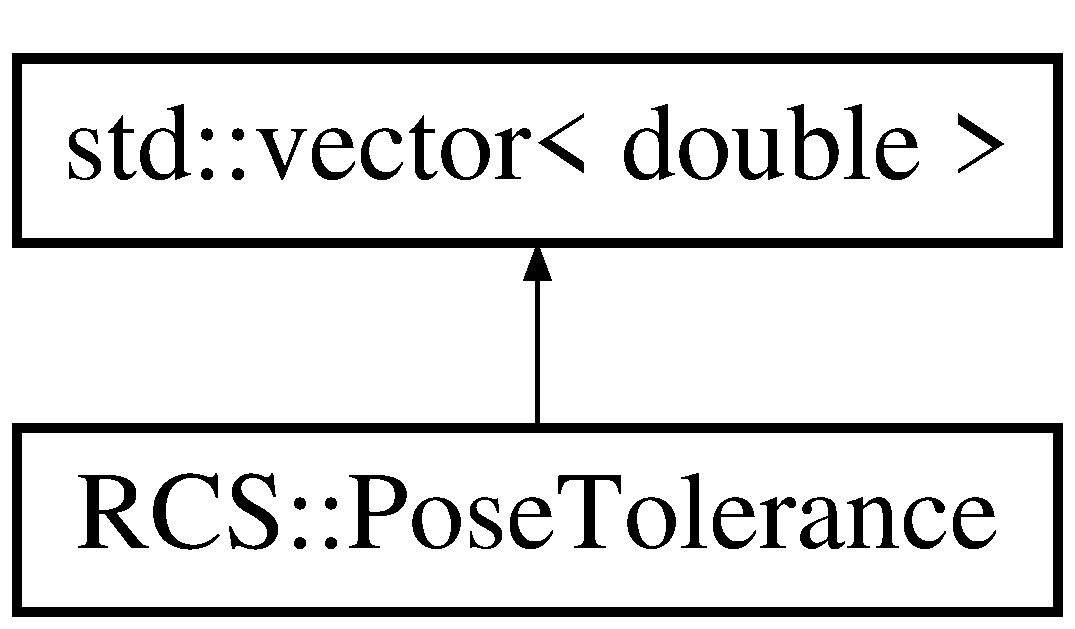
\includegraphics[height=2.000000cm]{structRCS_1_1PoseTolerance}
\end{center}
\end{figure}
\subsection*{Public Types}
\begin{DoxyCompactItemize}
\item 
enum \hyperlink{structRCS_1_1PoseTolerance_ab4307fac8693b1be023ed6b400ceac5b}{Type} \{ \hyperlink{structRCS_1_1PoseTolerance_ab4307fac8693b1be023ed6b400ceac5ba6b7feecf2cffe65d20a3d8226c7f06de}{P\-O\-S\-I\-T\-I\-O\-N} = 0, 
\hyperlink{structRCS_1_1PoseTolerance_ab4307fac8693b1be023ed6b400ceac5baa9a7358a420dc0961069428aedf2fd97}{O\-R\-I\-E\-N\-T\-A\-T\-I\-O\-N} = 1, 
\hyperlink{structRCS_1_1PoseTolerance_ab4307fac8693b1be023ed6b400ceac5ba214d30542fd89e624931dec916b4db68}{J\-O\-I\-N\-T} = 2
 \}
\end{DoxyCompactItemize}
\subsection*{Public Member Functions}
\begin{DoxyCompactItemize}
\item 
\hyperlink{structRCS_1_1PoseTolerance_adb9beae3f4967a164c207ef37cc2ce2f}{Pose\-Tolerance} ()
\end{DoxyCompactItemize}


\subsection{Member Enumeration Documentation}
\hypertarget{structRCS_1_1PoseTolerance_ab4307fac8693b1be023ed6b400ceac5b}{\index{R\-C\-S\-::\-Pose\-Tolerance@{R\-C\-S\-::\-Pose\-Tolerance}!Type@{Type}}
\index{Type@{Type}!RCS::PoseTolerance@{R\-C\-S\-::\-Pose\-Tolerance}}
\subsubsection[{Type}]{\setlength{\rightskip}{0pt plus 5cm}enum {\bf R\-C\-S\-::\-Pose\-Tolerance\-::\-Type}}}\label{structRCS_1_1PoseTolerance_ab4307fac8693b1be023ed6b400ceac5b}
\begin{Desc}
\item[Enumerator]\par
\begin{description}
\index{P\-O\-S\-I\-T\-I\-O\-N@{P\-O\-S\-I\-T\-I\-O\-N}!R\-C\-S\-::\-Pose\-Tolerance@{R\-C\-S\-::\-Pose\-Tolerance}}\index{R\-C\-S\-::\-Pose\-Tolerance@{R\-C\-S\-::\-Pose\-Tolerance}!P\-O\-S\-I\-T\-I\-O\-N@{P\-O\-S\-I\-T\-I\-O\-N}}\item[{\em 
\hypertarget{structRCS_1_1PoseTolerance_ab4307fac8693b1be023ed6b400ceac5ba6b7feecf2cffe65d20a3d8226c7f06de}{P\-O\-S\-I\-T\-I\-O\-N}\label{structRCS_1_1PoseTolerance_ab4307fac8693b1be023ed6b400ceac5ba6b7feecf2cffe65d20a3d8226c7f06de}
}]\index{O\-R\-I\-E\-N\-T\-A\-T\-I\-O\-N@{O\-R\-I\-E\-N\-T\-A\-T\-I\-O\-N}!R\-C\-S\-::\-Pose\-Tolerance@{R\-C\-S\-::\-Pose\-Tolerance}}\index{R\-C\-S\-::\-Pose\-Tolerance@{R\-C\-S\-::\-Pose\-Tolerance}!O\-R\-I\-E\-N\-T\-A\-T\-I\-O\-N@{O\-R\-I\-E\-N\-T\-A\-T\-I\-O\-N}}\item[{\em 
\hypertarget{structRCS_1_1PoseTolerance_ab4307fac8693b1be023ed6b400ceac5baa9a7358a420dc0961069428aedf2fd97}{O\-R\-I\-E\-N\-T\-A\-T\-I\-O\-N}\label{structRCS_1_1PoseTolerance_ab4307fac8693b1be023ed6b400ceac5baa9a7358a420dc0961069428aedf2fd97}
}]\index{J\-O\-I\-N\-T@{J\-O\-I\-N\-T}!R\-C\-S\-::\-Pose\-Tolerance@{R\-C\-S\-::\-Pose\-Tolerance}}\index{R\-C\-S\-::\-Pose\-Tolerance@{R\-C\-S\-::\-Pose\-Tolerance}!J\-O\-I\-N\-T@{J\-O\-I\-N\-T}}\item[{\em 
\hypertarget{structRCS_1_1PoseTolerance_ab4307fac8693b1be023ed6b400ceac5ba214d30542fd89e624931dec916b4db68}{J\-O\-I\-N\-T}\label{structRCS_1_1PoseTolerance_ab4307fac8693b1be023ed6b400ceac5ba214d30542fd89e624931dec916b4db68}
}]\end{description}
\end{Desc}


\subsection{Constructor \& Destructor Documentation}
\hypertarget{structRCS_1_1PoseTolerance_adb9beae3f4967a164c207ef37cc2ce2f}{\index{R\-C\-S\-::\-Pose\-Tolerance@{R\-C\-S\-::\-Pose\-Tolerance}!Pose\-Tolerance@{Pose\-Tolerance}}
\index{Pose\-Tolerance@{Pose\-Tolerance}!RCS::PoseTolerance@{R\-C\-S\-::\-Pose\-Tolerance}}
\subsubsection[{Pose\-Tolerance}]{\setlength{\rightskip}{0pt plus 5cm}R\-C\-S\-::\-Pose\-Tolerance\-::\-Pose\-Tolerance (
\begin{DoxyParamCaption}
{}
\end{DoxyParamCaption}
)\hspace{0.3cm}{\ttfamily [inline]}}}\label{structRCS_1_1PoseTolerance_adb9beae3f4967a164c207ef37cc2ce2f}


The documentation for this struct was generated from the following file\-:\begin{DoxyCompactItemize}
\item 
/usr/local/michalos/nistfanuc\-\_\-ws/src/nist\-\_\-fanuc/include/nist\-\_\-fanuc/\hyperlink{RCS_8h}{R\-C\-S.\-h}\end{DoxyCompactItemize}

\hypertarget{structRvizCheckers}{\section{Rviz\-Checkers Struct Reference}
\label{structRvizCheckers}\index{Rviz\-Checkers@{Rviz\-Checkers}}
}


{\ttfamily \#include $<$Checkerboard.\-h$>$}

\subsection*{Public Member Functions}
\begin{DoxyCompactItemize}
\item 
\hyperlink{structCheckers_1_1CheckersGame}{Checkers\-::\-Checkers\-Game} \& \hyperlink{structRvizCheckers_a31e53b9767a998d9bedd20998b5561ea}{Game} ()
\item 
\hyperlink{structRvizCheckers_a95baf9992cfeb3a3b874f147d2f3fe9d}{Rviz\-Checkers} (ros\-::\-Node\-Handle \&nh)
\item 
bool \& \hyperlink{structRvizCheckers_aa746d281199f9bf58ed7ef9325952e0b}{Ready} ()
\item 
void \hyperlink{structRvizCheckers_a4187bc58341cc86e3e8e0e8ffaf5d871}{callback} (const geometry\-\_\-msgs\-::\-Point\-Stamped\-::\-Const\-Ptr \&msg)
\item 
Eigen\-::\-Affine3d \hyperlink{structRvizCheckers_a2c48b30955cf52732df361bdea20a398}{Get\-Pose} (int row, int col)
\item 
double \hyperlink{structRvizCheckers_a2df1c2f1d7d4e279a507580dbc2a6dd4}{Row\-Offset} (int row)
\item 
double \hyperlink{structRvizCheckers_ae842a9dcbab4dbe573e14c114c3ffb0e}{Col\-Offset} (int col)
\item 
void \hyperlink{structRvizCheckers_a302d65fdf74e1c16df74c2aa8fc93197}{Rviz\-Setup} ()
\item 
void \hyperlink{structRvizCheckers_a19a88dafb8e2d58297635ca3115d04b7}{Set\-Checker\-Color} (\hyperlink{structCheckers_1_1Move}{Checkers\-::\-Move} m, rviz\-\_\-visual\-\_\-tools\-::colors color)
\item 
bool \hyperlink{structRvizCheckers_a8ea898a813fa22eac273d90b8f0e54d3}{Is\-King} (\hyperlink{structCheckers_1_1Move}{Checkers\-::\-Move} m)
\item 
bool \hyperlink{structRvizCheckers_a21f23e0708801d2f879f7a4112b4b770}{Is\-Already\-King} (\hyperlink{structCheckers_1_1Move}{Checkers\-::\-Move} m)
\item 
void \hyperlink{structRvizCheckers_adbed7ea9eb29ff3bc0c62bdf72e757c1}{Physical\-Move} (\hyperlink{classInlineRobotCommands}{Inline\-Robot\-Commands} \&robot, int player, int i, int j, \hyperlink{structCheckers_1_1Move}{Checkers\-::\-Move} m)
\item 
int \hyperlink{structRvizCheckers_a5e2dccff14bada10fe793dee9dce0ecb}{Player} ()
\item 
int \hyperlink{structRvizCheckers_ad3572edf478ea8ebdd3ff15d39a33974}{Opponent} ()
\item 
int \hyperlink{structRvizCheckers_ae658841732029ef2ef832bec586f8bf4}{Next\-Player} ()
\item 
bool \hyperlink{structRvizCheckers_a49e34dbb1c900f79f9b8287c458934ec}{Checkers\-Move} (int \&player, \hyperlink{structCheckers_1_1Move}{Checkers\-::\-Move} \&from, \hyperlink{structCheckers_1_1Move}{Checkers\-::\-Move} \&to)
\end{DoxyCompactItemize}
\subsection*{Public Attributes}
\begin{DoxyCompactItemize}
\item 
double \hyperlink{structRvizCheckers_af8fd72f18a7e6fd184015fd8fd338a52}{xoffset}
\item 
double \hyperlink{structRvizCheckers_aac2c25e5625cd2971d703c883137891a}{rowoffset}
\item 
double \hyperlink{structRvizCheckers_aeb28b7e85a132ec8fcd58feb4e8f7268}{yoffset}
\item 
double \hyperlink{structRvizCheckers_af3bd152c92bf85eac62af7dfe9da72d8}{offset}
\item 
double \hyperlink{structRvizCheckers_af5a8c18db31789f6e51c16ae72c4d3f0}{radius}
\item 
double \hyperlink{structRvizCheckers_a793ffa4bfbf3082cf581475711f7eb5a}{height}
\item 
\hyperlink{structCheckers_1_1CheckersGame}{Checkers\-::\-Checkers\-Game} \hyperlink{structRvizCheckers_a2805fb89f64f767e601bdd3d381600fe}{game}
\item 
int \hyperlink{structRvizCheckers_a69be787eb308ab029ecdb61a610af0c9}{curplayer}
\item 
ros\-::\-Subscriber \hyperlink{structRvizCheckers_a78950235459fcbaf0384072becf04838}{sub}
\item 
ros\-::\-Node\-Handle \& \hyperlink{structRvizCheckers_a60febb8e170bd5ce1b75b135a261a171}{\-\_\-nh}
\item 
bool \hyperlink{structRvizCheckers_a8539102352437ccaefc6622bb7dd81a0}{b\-Flag}
\end{DoxyCompactItemize}
\subsection*{Static Public Attributes}
\begin{DoxyCompactItemize}
\item 
static const int \hyperlink{structRvizCheckers_aad6dbe5aaca40570032f22a6e2242c9b}{rows} = 8
\item 
static const int \hyperlink{structRvizCheckers_a6a307940a101dca088951df5050bf62d}{cols} = 8
\end{DoxyCompactItemize}


\subsection{Constructor \& Destructor Documentation}
\hypertarget{structRvizCheckers_a95baf9992cfeb3a3b874f147d2f3fe9d}{\index{Rviz\-Checkers@{Rviz\-Checkers}!Rviz\-Checkers@{Rviz\-Checkers}}
\index{Rviz\-Checkers@{Rviz\-Checkers}!RvizCheckers@{Rviz\-Checkers}}
\subsubsection[{Rviz\-Checkers}]{\setlength{\rightskip}{0pt plus 5cm}Rviz\-Checkers\-::\-Rviz\-Checkers (
\begin{DoxyParamCaption}
\item[{ros\-::\-Node\-Handle \&}]{nh}
\end{DoxyParamCaption}
)\hspace{0.3cm}{\ttfamily [inline]}}}\label{structRvizCheckers_a95baf9992cfeb3a3b874f147d2f3fe9d}


\subsection{Member Function Documentation}
\hypertarget{structRvizCheckers_a4187bc58341cc86e3e8e0e8ffaf5d871}{\index{Rviz\-Checkers@{Rviz\-Checkers}!callback@{callback}}
\index{callback@{callback}!RvizCheckers@{Rviz\-Checkers}}
\subsubsection[{callback}]{\setlength{\rightskip}{0pt plus 5cm}void Rviz\-Checkers\-::callback (
\begin{DoxyParamCaption}
\item[{const geometry\-\_\-msgs\-::\-Point\-Stamped\-::\-Const\-Ptr \&}]{msg}
\end{DoxyParamCaption}
)\hspace{0.3cm}{\ttfamily [inline]}}}\label{structRvizCheckers_a4187bc58341cc86e3e8e0e8ffaf5d871}
\hypertarget{structRvizCheckers_a49e34dbb1c900f79f9b8287c458934ec}{\index{Rviz\-Checkers@{Rviz\-Checkers}!Checkers\-Move@{Checkers\-Move}}
\index{Checkers\-Move@{Checkers\-Move}!RvizCheckers@{Rviz\-Checkers}}
\subsubsection[{Checkers\-Move}]{\setlength{\rightskip}{0pt plus 5cm}bool Rviz\-Checkers\-::\-Checkers\-Move (
\begin{DoxyParamCaption}
\item[{int \&}]{player, }
\item[{{\bf Checkers\-::\-Move} \&}]{from, }
\item[{{\bf Checkers\-::\-Move} \&}]{to}
\end{DoxyParamCaption}
)\hspace{0.3cm}{\ttfamily [inline]}}}\label{structRvizCheckers_a49e34dbb1c900f79f9b8287c458934ec}
\hypertarget{structRvizCheckers_ae842a9dcbab4dbe573e14c114c3ffb0e}{\index{Rviz\-Checkers@{Rviz\-Checkers}!Col\-Offset@{Col\-Offset}}
\index{Col\-Offset@{Col\-Offset}!RvizCheckers@{Rviz\-Checkers}}
\subsubsection[{Col\-Offset}]{\setlength{\rightskip}{0pt plus 5cm}double Rviz\-Checkers\-::\-Col\-Offset (
\begin{DoxyParamCaption}
\item[{int}]{col}
\end{DoxyParamCaption}
)\hspace{0.3cm}{\ttfamily [inline]}}}\label{structRvizCheckers_ae842a9dcbab4dbe573e14c114c3ffb0e}
\hypertarget{structRvizCheckers_a31e53b9767a998d9bedd20998b5561ea}{\index{Rviz\-Checkers@{Rviz\-Checkers}!Game@{Game}}
\index{Game@{Game}!RvizCheckers@{Rviz\-Checkers}}
\subsubsection[{Game}]{\setlength{\rightskip}{0pt plus 5cm}{\bf Checkers\-::\-Checkers\-Game}\& Rviz\-Checkers\-::\-Game (
\begin{DoxyParamCaption}
{}
\end{DoxyParamCaption}
)\hspace{0.3cm}{\ttfamily [inline]}}}\label{structRvizCheckers_a31e53b9767a998d9bedd20998b5561ea}
\hypertarget{structRvizCheckers_a2c48b30955cf52732df361bdea20a398}{\index{Rviz\-Checkers@{Rviz\-Checkers}!Get\-Pose@{Get\-Pose}}
\index{Get\-Pose@{Get\-Pose}!RvizCheckers@{Rviz\-Checkers}}
\subsubsection[{Get\-Pose}]{\setlength{\rightskip}{0pt plus 5cm}Eigen\-::\-Affine3d Rviz\-Checkers\-::\-Get\-Pose (
\begin{DoxyParamCaption}
\item[{int}]{row, }
\item[{int}]{col}
\end{DoxyParamCaption}
)\hspace{0.3cm}{\ttfamily [inline]}}}\label{structRvizCheckers_a2c48b30955cf52732df361bdea20a398}
\hypertarget{structRvizCheckers_a21f23e0708801d2f879f7a4112b4b770}{\index{Rviz\-Checkers@{Rviz\-Checkers}!Is\-Already\-King@{Is\-Already\-King}}
\index{Is\-Already\-King@{Is\-Already\-King}!RvizCheckers@{Rviz\-Checkers}}
\subsubsection[{Is\-Already\-King}]{\setlength{\rightskip}{0pt plus 5cm}bool Rviz\-Checkers\-::\-Is\-Already\-King (
\begin{DoxyParamCaption}
\item[{{\bf Checkers\-::\-Move}}]{m}
\end{DoxyParamCaption}
)\hspace{0.3cm}{\ttfamily [inline]}}}\label{structRvizCheckers_a21f23e0708801d2f879f7a4112b4b770}
\hypertarget{structRvizCheckers_a8ea898a813fa22eac273d90b8f0e54d3}{\index{Rviz\-Checkers@{Rviz\-Checkers}!Is\-King@{Is\-King}}
\index{Is\-King@{Is\-King}!RvizCheckers@{Rviz\-Checkers}}
\subsubsection[{Is\-King}]{\setlength{\rightskip}{0pt plus 5cm}bool Rviz\-Checkers\-::\-Is\-King (
\begin{DoxyParamCaption}
\item[{{\bf Checkers\-::\-Move}}]{m}
\end{DoxyParamCaption}
)\hspace{0.3cm}{\ttfamily [inline]}}}\label{structRvizCheckers_a8ea898a813fa22eac273d90b8f0e54d3}
\hypertarget{structRvizCheckers_ae658841732029ef2ef832bec586f8bf4}{\index{Rviz\-Checkers@{Rviz\-Checkers}!Next\-Player@{Next\-Player}}
\index{Next\-Player@{Next\-Player}!RvizCheckers@{Rviz\-Checkers}}
\subsubsection[{Next\-Player}]{\setlength{\rightskip}{0pt plus 5cm}int Rviz\-Checkers\-::\-Next\-Player (
\begin{DoxyParamCaption}
{}
\end{DoxyParamCaption}
)\hspace{0.3cm}{\ttfamily [inline]}}}\label{structRvizCheckers_ae658841732029ef2ef832bec586f8bf4}
\hypertarget{structRvizCheckers_ad3572edf478ea8ebdd3ff15d39a33974}{\index{Rviz\-Checkers@{Rviz\-Checkers}!Opponent@{Opponent}}
\index{Opponent@{Opponent}!RvizCheckers@{Rviz\-Checkers}}
\subsubsection[{Opponent}]{\setlength{\rightskip}{0pt plus 5cm}int Rviz\-Checkers\-::\-Opponent (
\begin{DoxyParamCaption}
{}
\end{DoxyParamCaption}
)\hspace{0.3cm}{\ttfamily [inline]}}}\label{structRvizCheckers_ad3572edf478ea8ebdd3ff15d39a33974}
\hypertarget{structRvizCheckers_adbed7ea9eb29ff3bc0c62bdf72e757c1}{\index{Rviz\-Checkers@{Rviz\-Checkers}!Physical\-Move@{Physical\-Move}}
\index{Physical\-Move@{Physical\-Move}!RvizCheckers@{Rviz\-Checkers}}
\subsubsection[{Physical\-Move}]{\setlength{\rightskip}{0pt plus 5cm}void Rviz\-Checkers\-::\-Physical\-Move (
\begin{DoxyParamCaption}
\item[{{\bf Inline\-Robot\-Commands} \&}]{robot, }
\item[{int}]{player, }
\item[{int}]{i, }
\item[{int}]{j, }
\item[{{\bf Checkers\-::\-Move}}]{m}
\end{DoxyParamCaption}
)\hspace{0.3cm}{\ttfamily [inline]}}}\label{structRvizCheckers_adbed7ea9eb29ff3bc0c62bdf72e757c1}
\hypertarget{structRvizCheckers_a5e2dccff14bada10fe793dee9dce0ecb}{\index{Rviz\-Checkers@{Rviz\-Checkers}!Player@{Player}}
\index{Player@{Player}!RvizCheckers@{Rviz\-Checkers}}
\subsubsection[{Player}]{\setlength{\rightskip}{0pt plus 5cm}int Rviz\-Checkers\-::\-Player (
\begin{DoxyParamCaption}
{}
\end{DoxyParamCaption}
)\hspace{0.3cm}{\ttfamily [inline]}}}\label{structRvizCheckers_a5e2dccff14bada10fe793dee9dce0ecb}
\hypertarget{structRvizCheckers_aa746d281199f9bf58ed7ef9325952e0b}{\index{Rviz\-Checkers@{Rviz\-Checkers}!Ready@{Ready}}
\index{Ready@{Ready}!RvizCheckers@{Rviz\-Checkers}}
\subsubsection[{Ready}]{\setlength{\rightskip}{0pt plus 5cm}bool\& Rviz\-Checkers\-::\-Ready (
\begin{DoxyParamCaption}
{}
\end{DoxyParamCaption}
)\hspace{0.3cm}{\ttfamily [inline]}}}\label{structRvizCheckers_aa746d281199f9bf58ed7ef9325952e0b}
\hypertarget{structRvizCheckers_a2df1c2f1d7d4e279a507580dbc2a6dd4}{\index{Rviz\-Checkers@{Rviz\-Checkers}!Row\-Offset@{Row\-Offset}}
\index{Row\-Offset@{Row\-Offset}!RvizCheckers@{Rviz\-Checkers}}
\subsubsection[{Row\-Offset}]{\setlength{\rightskip}{0pt plus 5cm}double Rviz\-Checkers\-::\-Row\-Offset (
\begin{DoxyParamCaption}
\item[{int}]{row}
\end{DoxyParamCaption}
)\hspace{0.3cm}{\ttfamily [inline]}}}\label{structRvizCheckers_a2df1c2f1d7d4e279a507580dbc2a6dd4}
\hypertarget{structRvizCheckers_a302d65fdf74e1c16df74c2aa8fc93197}{\index{Rviz\-Checkers@{Rviz\-Checkers}!Rviz\-Setup@{Rviz\-Setup}}
\index{Rviz\-Setup@{Rviz\-Setup}!RvizCheckers@{Rviz\-Checkers}}
\subsubsection[{Rviz\-Setup}]{\setlength{\rightskip}{0pt plus 5cm}void Rviz\-Checkers\-::\-Rviz\-Setup (
\begin{DoxyParamCaption}
{}
\end{DoxyParamCaption}
)\hspace{0.3cm}{\ttfamily [inline]}}}\label{structRvizCheckers_a302d65fdf74e1c16df74c2aa8fc93197}
\hypertarget{structRvizCheckers_a19a88dafb8e2d58297635ca3115d04b7}{\index{Rviz\-Checkers@{Rviz\-Checkers}!Set\-Checker\-Color@{Set\-Checker\-Color}}
\index{Set\-Checker\-Color@{Set\-Checker\-Color}!RvizCheckers@{Rviz\-Checkers}}
\subsubsection[{Set\-Checker\-Color}]{\setlength{\rightskip}{0pt plus 5cm}void Rviz\-Checkers\-::\-Set\-Checker\-Color (
\begin{DoxyParamCaption}
\item[{{\bf Checkers\-::\-Move}}]{m, }
\item[{rviz\-\_\-visual\-\_\-tools\-::colors}]{color}
\end{DoxyParamCaption}
)\hspace{0.3cm}{\ttfamily [inline]}}}\label{structRvizCheckers_a19a88dafb8e2d58297635ca3115d04b7}


\subsection{Member Data Documentation}
\hypertarget{structRvizCheckers_a60febb8e170bd5ce1b75b135a261a171}{\index{Rviz\-Checkers@{Rviz\-Checkers}!\-\_\-nh@{\-\_\-nh}}
\index{\-\_\-nh@{\-\_\-nh}!RvizCheckers@{Rviz\-Checkers}}
\subsubsection[{\-\_\-nh}]{\setlength{\rightskip}{0pt plus 5cm}ros\-::\-Node\-Handle\& Rviz\-Checkers\-::\-\_\-nh}}\label{structRvizCheckers_a60febb8e170bd5ce1b75b135a261a171}
\hypertarget{structRvizCheckers_a8539102352437ccaefc6622bb7dd81a0}{\index{Rviz\-Checkers@{Rviz\-Checkers}!b\-Flag@{b\-Flag}}
\index{b\-Flag@{b\-Flag}!RvizCheckers@{Rviz\-Checkers}}
\subsubsection[{b\-Flag}]{\setlength{\rightskip}{0pt plus 5cm}bool Rviz\-Checkers\-::b\-Flag}}\label{structRvizCheckers_a8539102352437ccaefc6622bb7dd81a0}
\hypertarget{structRvizCheckers_a6a307940a101dca088951df5050bf62d}{\index{Rviz\-Checkers@{Rviz\-Checkers}!cols@{cols}}
\index{cols@{cols}!RvizCheckers@{Rviz\-Checkers}}
\subsubsection[{cols}]{\setlength{\rightskip}{0pt plus 5cm}const int Rviz\-Checkers\-::cols = 8\hspace{0.3cm}{\ttfamily [static]}}}\label{structRvizCheckers_a6a307940a101dca088951df5050bf62d}
\hypertarget{structRvizCheckers_a69be787eb308ab029ecdb61a610af0c9}{\index{Rviz\-Checkers@{Rviz\-Checkers}!curplayer@{curplayer}}
\index{curplayer@{curplayer}!RvizCheckers@{Rviz\-Checkers}}
\subsubsection[{curplayer}]{\setlength{\rightskip}{0pt plus 5cm}int Rviz\-Checkers\-::curplayer}}\label{structRvizCheckers_a69be787eb308ab029ecdb61a610af0c9}
\hypertarget{structRvizCheckers_a2805fb89f64f767e601bdd3d381600fe}{\index{Rviz\-Checkers@{Rviz\-Checkers}!game@{game}}
\index{game@{game}!RvizCheckers@{Rviz\-Checkers}}
\subsubsection[{game}]{\setlength{\rightskip}{0pt plus 5cm}{\bf Checkers\-::\-Checkers\-Game} Rviz\-Checkers\-::game}}\label{structRvizCheckers_a2805fb89f64f767e601bdd3d381600fe}
\hypertarget{structRvizCheckers_a793ffa4bfbf3082cf581475711f7eb5a}{\index{Rviz\-Checkers@{Rviz\-Checkers}!height@{height}}
\index{height@{height}!RvizCheckers@{Rviz\-Checkers}}
\subsubsection[{height}]{\setlength{\rightskip}{0pt plus 5cm}double Rviz\-Checkers\-::height}}\label{structRvizCheckers_a793ffa4bfbf3082cf581475711f7eb5a}
\hypertarget{structRvizCheckers_af3bd152c92bf85eac62af7dfe9da72d8}{\index{Rviz\-Checkers@{Rviz\-Checkers}!offset@{offset}}
\index{offset@{offset}!RvizCheckers@{Rviz\-Checkers}}
\subsubsection[{offset}]{\setlength{\rightskip}{0pt plus 5cm}double Rviz\-Checkers\-::offset}}\label{structRvizCheckers_af3bd152c92bf85eac62af7dfe9da72d8}
\hypertarget{structRvizCheckers_af5a8c18db31789f6e51c16ae72c4d3f0}{\index{Rviz\-Checkers@{Rviz\-Checkers}!radius@{radius}}
\index{radius@{radius}!RvizCheckers@{Rviz\-Checkers}}
\subsubsection[{radius}]{\setlength{\rightskip}{0pt plus 5cm}double Rviz\-Checkers\-::radius}}\label{structRvizCheckers_af5a8c18db31789f6e51c16ae72c4d3f0}
\hypertarget{structRvizCheckers_aac2c25e5625cd2971d703c883137891a}{\index{Rviz\-Checkers@{Rviz\-Checkers}!rowoffset@{rowoffset}}
\index{rowoffset@{rowoffset}!RvizCheckers@{Rviz\-Checkers}}
\subsubsection[{rowoffset}]{\setlength{\rightskip}{0pt plus 5cm}double Rviz\-Checkers\-::rowoffset}}\label{structRvizCheckers_aac2c25e5625cd2971d703c883137891a}
\hypertarget{structRvizCheckers_aad6dbe5aaca40570032f22a6e2242c9b}{\index{Rviz\-Checkers@{Rviz\-Checkers}!rows@{rows}}
\index{rows@{rows}!RvizCheckers@{Rviz\-Checkers}}
\subsubsection[{rows}]{\setlength{\rightskip}{0pt plus 5cm}const int Rviz\-Checkers\-::rows = 8\hspace{0.3cm}{\ttfamily [static]}}}\label{structRvizCheckers_aad6dbe5aaca40570032f22a6e2242c9b}
\hypertarget{structRvizCheckers_a78950235459fcbaf0384072becf04838}{\index{Rviz\-Checkers@{Rviz\-Checkers}!sub@{sub}}
\index{sub@{sub}!RvizCheckers@{Rviz\-Checkers}}
\subsubsection[{sub}]{\setlength{\rightskip}{0pt plus 5cm}ros\-::\-Subscriber Rviz\-Checkers\-::sub}}\label{structRvizCheckers_a78950235459fcbaf0384072becf04838}
\hypertarget{structRvizCheckers_af8fd72f18a7e6fd184015fd8fd338a52}{\index{Rviz\-Checkers@{Rviz\-Checkers}!xoffset@{xoffset}}
\index{xoffset@{xoffset}!RvizCheckers@{Rviz\-Checkers}}
\subsubsection[{xoffset}]{\setlength{\rightskip}{0pt plus 5cm}double Rviz\-Checkers\-::xoffset}}\label{structRvizCheckers_af8fd72f18a7e6fd184015fd8fd338a52}
\hypertarget{structRvizCheckers_aeb28b7e85a132ec8fcd58feb4e8f7268}{\index{Rviz\-Checkers@{Rviz\-Checkers}!yoffset@{yoffset}}
\index{yoffset@{yoffset}!RvizCheckers@{Rviz\-Checkers}}
\subsubsection[{yoffset}]{\setlength{\rightskip}{0pt plus 5cm}double Rviz\-Checkers\-::yoffset}}\label{structRvizCheckers_aeb28b7e85a132ec8fcd58feb4e8f7268}


The documentation for this struct was generated from the following file\-:\begin{DoxyCompactItemize}
\item 
/usr/local/michalos/nistfanuc\-\_\-ws/src/nist\-\_\-fanuc/include/nist\-\_\-fanuc/\hyperlink{Checkerboard_8h}{Checkerboard.\-h}\end{DoxyCompactItemize}

\hypertarget{classRvizDemo}{\section{Rviz\-Demo Class Reference}
\label{classRvizDemo}\index{Rviz\-Demo@{Rviz\-Demo}}
}


{\ttfamily \#include $<$Demo.\-h$>$}

\subsection*{Public Member Functions}
\begin{DoxyCompactItemize}
\item 
\hyperlink{classRvizDemo_a36e6ed2ae50852b13def36b58deedbc1}{Rviz\-Demo} (ros\-::\-Node\-Handle \&nh)
\item 
bool \hyperlink{classRvizDemo_af11434c2365d0ad9a7c4f1ba81327f49}{Ready} ()
\item 
void \hyperlink{classRvizDemo_abc8d8dce2484e9c932d9b42ce60080e1}{Unset} ()
\item 
void \hyperlink{classRvizDemo_a71d08ff849dcfab2acdedd88268ffef6}{callback} (const geometry\-\_\-msgs\-::\-Point\-Stamped\-::\-Const\-Ptr \&msg)
\end{DoxyCompactItemize}
\subsection*{Protected Attributes}
\begin{DoxyCompactItemize}
\item 
ros\-::\-Subscriber \hyperlink{classRvizDemo_a47f574e38565699efdb24fc628722716}{sub}
\item 
ros\-::\-Node\-Handle \& \hyperlink{classRvizDemo_afbd5562859f25a7747968cd9375bb3d7}{\-\_\-nh}
\item 
bool \hyperlink{classRvizDemo_a559916f367fa110e12c09d370888925f}{b\-Flag}
\end{DoxyCompactItemize}
\subsection*{Static Protected Attributes}
\begin{DoxyCompactItemize}
\item 
static boost\-::mutex \hyperlink{classRvizDemo_a91fefdf56048c3f7c9a9391e80e06f21}{\-\_\-flag\-\_\-mutex}
\end{DoxyCompactItemize}


\subsection{Constructor \& Destructor Documentation}
\hypertarget{classRvizDemo_a36e6ed2ae50852b13def36b58deedbc1}{\index{Rviz\-Demo@{Rviz\-Demo}!Rviz\-Demo@{Rviz\-Demo}}
\index{Rviz\-Demo@{Rviz\-Demo}!RvizDemo@{Rviz\-Demo}}
\subsubsection[{Rviz\-Demo}]{\setlength{\rightskip}{0pt plus 5cm}Rviz\-Demo\-::\-Rviz\-Demo (
\begin{DoxyParamCaption}
\item[{ros\-::\-Node\-Handle \&}]{nh}
\end{DoxyParamCaption}
)\hspace{0.3cm}{\ttfamily [inline]}}}\label{classRvizDemo_a36e6ed2ae50852b13def36b58deedbc1}


\subsection{Member Function Documentation}
\hypertarget{classRvizDemo_a71d08ff849dcfab2acdedd88268ffef6}{\index{Rviz\-Demo@{Rviz\-Demo}!callback@{callback}}
\index{callback@{callback}!RvizDemo@{Rviz\-Demo}}
\subsubsection[{callback}]{\setlength{\rightskip}{0pt plus 5cm}void Rviz\-Demo\-::callback (
\begin{DoxyParamCaption}
\item[{const geometry\-\_\-msgs\-::\-Point\-Stamped\-::\-Const\-Ptr \&}]{msg}
\end{DoxyParamCaption}
)\hspace{0.3cm}{\ttfamily [inline]}}}\label{classRvizDemo_a71d08ff849dcfab2acdedd88268ffef6}
\hypertarget{classRvizDemo_af11434c2365d0ad9a7c4f1ba81327f49}{\index{Rviz\-Demo@{Rviz\-Demo}!Ready@{Ready}}
\index{Ready@{Ready}!RvizDemo@{Rviz\-Demo}}
\subsubsection[{Ready}]{\setlength{\rightskip}{0pt plus 5cm}bool Rviz\-Demo\-::\-Ready (
\begin{DoxyParamCaption}
{}
\end{DoxyParamCaption}
)\hspace{0.3cm}{\ttfamily [inline]}}}\label{classRvizDemo_af11434c2365d0ad9a7c4f1ba81327f49}
\hypertarget{classRvizDemo_abc8d8dce2484e9c932d9b42ce60080e1}{\index{Rviz\-Demo@{Rviz\-Demo}!Unset@{Unset}}
\index{Unset@{Unset}!RvizDemo@{Rviz\-Demo}}
\subsubsection[{Unset}]{\setlength{\rightskip}{0pt plus 5cm}void Rviz\-Demo\-::\-Unset (
\begin{DoxyParamCaption}
{}
\end{DoxyParamCaption}
)\hspace{0.3cm}{\ttfamily [inline]}}}\label{classRvizDemo_abc8d8dce2484e9c932d9b42ce60080e1}


\subsection{Member Data Documentation}
\hypertarget{classRvizDemo_a91fefdf56048c3f7c9a9391e80e06f21}{\index{Rviz\-Demo@{Rviz\-Demo}!\-\_\-flag\-\_\-mutex@{\-\_\-flag\-\_\-mutex}}
\index{\-\_\-flag\-\_\-mutex@{\-\_\-flag\-\_\-mutex}!RvizDemo@{Rviz\-Demo}}
\subsubsection[{\-\_\-flag\-\_\-mutex}]{\setlength{\rightskip}{0pt plus 5cm}boost\-::mutex Rviz\-Demo\-::\-\_\-flag\-\_\-mutex\hspace{0.3cm}{\ttfamily [static]}, {\ttfamily [protected]}}}\label{classRvizDemo_a91fefdf56048c3f7c9a9391e80e06f21}
\hypertarget{classRvizDemo_afbd5562859f25a7747968cd9375bb3d7}{\index{Rviz\-Demo@{Rviz\-Demo}!\-\_\-nh@{\-\_\-nh}}
\index{\-\_\-nh@{\-\_\-nh}!RvizDemo@{Rviz\-Demo}}
\subsubsection[{\-\_\-nh}]{\setlength{\rightskip}{0pt plus 5cm}ros\-::\-Node\-Handle\& Rviz\-Demo\-::\-\_\-nh\hspace{0.3cm}{\ttfamily [protected]}}}\label{classRvizDemo_afbd5562859f25a7747968cd9375bb3d7}
\hypertarget{classRvizDemo_a559916f367fa110e12c09d370888925f}{\index{Rviz\-Demo@{Rviz\-Demo}!b\-Flag@{b\-Flag}}
\index{b\-Flag@{b\-Flag}!RvizDemo@{Rviz\-Demo}}
\subsubsection[{b\-Flag}]{\setlength{\rightskip}{0pt plus 5cm}bool Rviz\-Demo\-::b\-Flag\hspace{0.3cm}{\ttfamily [protected]}}}\label{classRvizDemo_a559916f367fa110e12c09d370888925f}
\hypertarget{classRvizDemo_a47f574e38565699efdb24fc628722716}{\index{Rviz\-Demo@{Rviz\-Demo}!sub@{sub}}
\index{sub@{sub}!RvizDemo@{Rviz\-Demo}}
\subsubsection[{sub}]{\setlength{\rightskip}{0pt plus 5cm}ros\-::\-Subscriber Rviz\-Demo\-::sub\hspace{0.3cm}{\ttfamily [protected]}}}\label{classRvizDemo_a47f574e38565699efdb24fc628722716}


The documentation for this class was generated from the following files\-:\begin{DoxyCompactItemize}
\item 
/usr/local/michalos/nistfanuc\-\_\-ws/src/nist\-\_\-fanuc/include/nist\-\_\-fanuc/\hyperlink{Demo_8h}{Demo.\-h}\item 
/usr/local/michalos/nistfanuc\-\_\-ws/src/nist\-\_\-fanuc/src/\hyperlink{Demo_8cpp}{Demo.\-cpp}\end{DoxyCompactItemize}

\hypertarget{structSonOfRvizVisualTools}{\section{Son\-Of\-Rviz\-Visual\-Tools Struct Reference}
\label{structSonOfRvizVisualTools}\index{Son\-Of\-Rviz\-Visual\-Tools@{Son\-Of\-Rviz\-Visual\-Tools}}
}


{\ttfamily \#include $<$Scene.\-h$>$}

Inheritance diagram for Son\-Of\-Rviz\-Visual\-Tools\-:\begin{figure}[H]
\begin{center}
\leavevmode
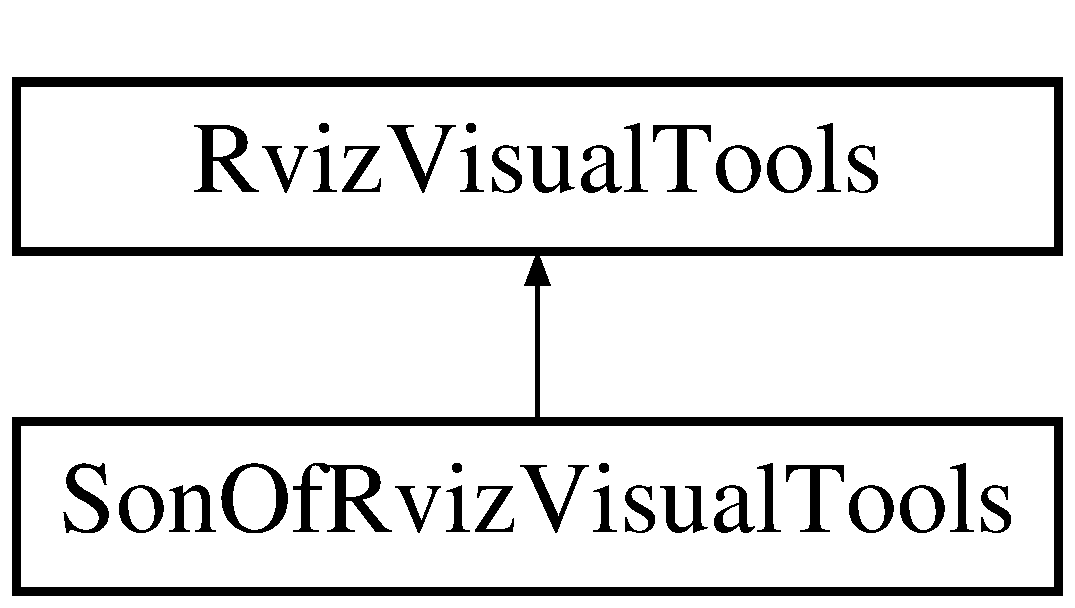
\includegraphics[height=2.000000cm]{structSonOfRvizVisualTools}
\end{center}
\end{figure}
\subsection*{Public Member Functions}
\begin{DoxyCompactItemize}
\item 
\hyperlink{structSonOfRvizVisualTools_a64d3128f74b491a1f9d522fd29473781}{Son\-Of\-Rviz\-Visual\-Tools} (const std\-::string \&base\-\_\-frame)
\item 
size\-\_\-t \hyperlink{structSonOfRvizVisualTools_a416ce0995acbb2bd009527453613629a}{Get\-Cylinder\-Id} ()
\end{DoxyCompactItemize}


\subsection{Constructor \& Destructor Documentation}
\hypertarget{structSonOfRvizVisualTools_a64d3128f74b491a1f9d522fd29473781}{\index{Son\-Of\-Rviz\-Visual\-Tools@{Son\-Of\-Rviz\-Visual\-Tools}!Son\-Of\-Rviz\-Visual\-Tools@{Son\-Of\-Rviz\-Visual\-Tools}}
\index{Son\-Of\-Rviz\-Visual\-Tools@{Son\-Of\-Rviz\-Visual\-Tools}!SonOfRvizVisualTools@{Son\-Of\-Rviz\-Visual\-Tools}}
\subsubsection[{Son\-Of\-Rviz\-Visual\-Tools}]{\setlength{\rightskip}{0pt plus 5cm}Son\-Of\-Rviz\-Visual\-Tools\-::\-Son\-Of\-Rviz\-Visual\-Tools (
\begin{DoxyParamCaption}
\item[{const std\-::string \&}]{base\-\_\-frame}
\end{DoxyParamCaption}
)\hspace{0.3cm}{\ttfamily [inline]}}}\label{structSonOfRvizVisualTools_a64d3128f74b491a1f9d522fd29473781}


\subsection{Member Function Documentation}
\hypertarget{structSonOfRvizVisualTools_a416ce0995acbb2bd009527453613629a}{\index{Son\-Of\-Rviz\-Visual\-Tools@{Son\-Of\-Rviz\-Visual\-Tools}!Get\-Cylinder\-Id@{Get\-Cylinder\-Id}}
\index{Get\-Cylinder\-Id@{Get\-Cylinder\-Id}!SonOfRvizVisualTools@{Son\-Of\-Rviz\-Visual\-Tools}}
\subsubsection[{Get\-Cylinder\-Id}]{\setlength{\rightskip}{0pt plus 5cm}size\-\_\-t Son\-Of\-Rviz\-Visual\-Tools\-::\-Get\-Cylinder\-Id (
\begin{DoxyParamCaption}
{}
\end{DoxyParamCaption}
)\hspace{0.3cm}{\ttfamily [inline]}}}\label{structSonOfRvizVisualTools_a416ce0995acbb2bd009527453613629a}


The documentation for this struct was generated from the following file\-:\begin{DoxyCompactItemize}
\item 
/usr/local/michalos/nistfanuc\-\_\-ws/src/nist\-\_\-fanuc/include/nist\-\_\-fanuc/\hyperlink{Scene_8h}{Scene.\-h}\end{DoxyCompactItemize}

\hypertarget{classRCS_1_1Thread}{\section{R\-C\-S\-:\-:Thread Class Reference}
\label{classRCS_1_1Thread}\index{R\-C\-S\-::\-Thread@{R\-C\-S\-::\-Thread}}
}


\hyperlink{classRCS_1_1Thread}{Thread} is an \hyperlink{namespaceRCS}{R\-C\-S} ulapi equivalent for a timed thread. Given a cycle time, the thread provides a wait function to sleep to exactly the amount of the thread cycle time. It keeps track of busy/idle time for diagnostic purposes. \par
 Notes\-: \href{https://www.quantnet.com/threads/c-multithreading-in-boost.10028/}{\tt https\-://www.\-quantnet.\-com/threads/c-\/multithreading-\/in-\/boost.\-10028/}.  




{\ttfamily \#include $<$R\-C\-S\-Thread\-Template.\-h$>$}

Inheritance diagram for R\-C\-S\-:\-:Thread\-:\begin{figure}[H]
\begin{center}
\leavevmode
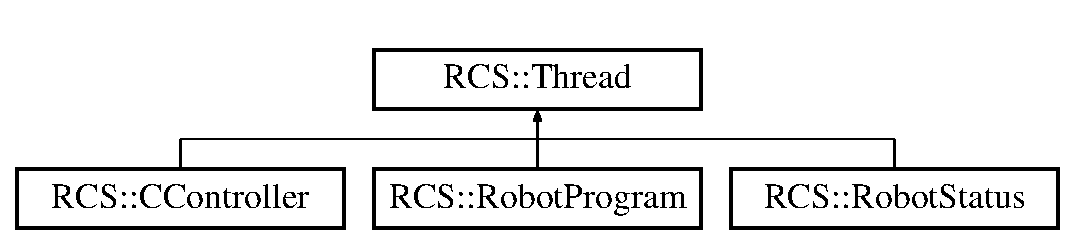
\includegraphics[height=2.000000cm]{classRCS_1_1Thread}
\end{center}
\end{figure}
\subsection*{Public Member Functions}
\begin{DoxyCompactItemize}
\item 
\hyperlink{classRCS_1_1Thread_a3f5e86f11c0b8fc3aa4728549b1b7249}{Thread} (double cycletime)
\begin{DoxyCompactList}\small\item\em Constructor of thread, that takes cycle time as input. \end{DoxyCompactList}\item 
\hyperlink{classRCS_1_1Thread_a7b91358afd5f9609b3a6b5b32f9a89aa}{$\sim$\-Thread} ()
\begin{DoxyCompactList}\small\item\em Destructor of thread, makes sure thread has stopped. \end{DoxyCompactList}\item 
std\-::string \& \hyperlink{classRCS_1_1Thread_a2db2a8e8dea3c4e502e8d6adbbf05724}{Name} ()
\begin{DoxyCompactList}\small\item\em Name returns name of thread. \end{DoxyCompactList}\item 
void \hyperlink{classRCS_1_1Thread_a5f7209d2edfa23588f6adc74bbfb8f07}{Join} ()
\begin{DoxyCompactList}\small\item\em Uses boost thread join routine. \end{DoxyCompactList}\item 
virtual void \hyperlink{classRCS_1_1Thread_a53ee19c04d064c9a23f0909cf9a4b2cc}{Init} ()
\begin{DoxyCompactList}\small\item\em Init function called before \hyperlink{classRCS_1_1Thread_a78aec7128f4fbf5d6859ceb09f9f9ae1}{Action()} loop. \end{DoxyCompactList}\item 
virtual void \hyperlink{classRCS_1_1Thread_a8b932e4130f18d9747407fe70a87332a}{Cleanup} ()
\begin{DoxyCompactList}\small\item\em Cleanup function called after \hyperlink{classRCS_1_1Thread_a78aec7128f4fbf5d6859ceb09f9f9ae1}{Action()} loop done. \end{DoxyCompactList}\item 
virtual int \hyperlink{classRCS_1_1Thread_a78aec7128f4fbf5d6859ceb09f9f9ae1}{Action} ()
\begin{DoxyCompactList}\small\item\em Action override function called every cycle. \end{DoxyCompactList}\item 
void \hyperlink{classRCS_1_1Thread_a86b50ec69dd0baeda270b115d72c1c15}{Start} ()
\begin{DoxyCompactList}\small\item\em Start starts the thread which call \hyperlink{classRCS_1_1Thread_a53ee19c04d064c9a23f0909cf9a4b2cc}{Init()}, and then does \hyperlink{classRCS_1_1Thread_a78aec7128f4fbf5d6859ceb09f9f9ae1}{Action()} loop. \end{DoxyCompactList}\item 
void \hyperlink{classRCS_1_1Thread_ae0c4a68567ab695f4b7daf755ab874d6}{Stop} (bool b\-Wait=false)
\begin{DoxyCompactList}\small\item\em Stop stops the thread loop. \end{DoxyCompactList}\item 
void \hyperlink{classRCS_1_1Thread_a6a5f86951a6b1fa10bc90844366bd23e}{Suspend} ()
\begin{DoxyCompactList}\small\item\em Suspend stops the thread loop until restarted with \hyperlink{classRCS_1_1Thread_adf2b3b0fc8b643b1fd2b6f28f30c7a2e}{Resume()}. \end{DoxyCompactList}\item 
void \hyperlink{classRCS_1_1Thread_adf2b3b0fc8b643b1fd2b6f28f30c7a2e}{Resume} ()
\begin{DoxyCompactList}\small\item\em Resume resume execution of the thread loop stopped with \hyperlink{classRCS_1_1Thread_a6a5f86951a6b1fa10bc90844366bd23e}{Suspend()}. \end{DoxyCompactList}\item 
double \hyperlink{classRCS_1_1Thread_a0de02ea91ce412d0770452dcd2256e35}{Load} ()
\begin{DoxyCompactList}\small\item\em Load returns the load of the thread cycle. \end{DoxyCompactList}\item 
double \& \hyperlink{classRCS_1_1Thread_a1738e943d3ca8a9861941610db819161}{Cycle\-Time} ()
\begin{DoxyCompactList}\small\item\em Cycle\-Time returns the cycle time of the thread cycle in seconds. \end{DoxyCompactList}\item 
void \hyperlink{classRCS_1_1Thread_a4bb0d136529374782030bf1bd19cad6d}{Set\-Debug\-Level} (int n)
\begin{DoxyCompactList}\small\item\em Set\-Debug\-Level sets the debugging level of the thread. \end{DoxyCompactList}\item 
int \& \hyperlink{classRCS_1_1Thread_abe304b8316eb45e0b01c1104376fbc41}{Debug\-Level} ()
\begin{DoxyCompactList}\small\item\em Debug\-Level returns the debugging level of the thread. \end{DoxyCompactList}\item 
void \hyperlink{classRCS_1_1Thread_a12ff1372b891db600b094d628e606045}{Cycle} ()
\begin{DoxyCompactList}\small\item\em Cycle is the thread main function. It calls init, action, and cleanup. After each cycle waits exa\-\_\-newccctly amount given by cycle time. \end{DoxyCompactList}\end{DoxyCompactItemize}
\subsection*{Static Public Member Functions}
\begin{DoxyCompactItemize}
\item 
static boost\-::thread\-\_\-group \& \hyperlink{classRCS_1_1Thread_ae3269a75272f142bc8423ecef1d98d12}{Thread\-Group} ()
\begin{DoxyCompactList}\small\item\em Thread\-Group is a static definition of boost thread group. \end{DoxyCompactList}\item 
static std\-::vector$<$ \hyperlink{classRCS_1_1Thread}{Thread} $\ast$ $>$ \& \hyperlink{classRCS_1_1Thread_a9accd6dbb70083160c9d1aa21585b5f9}{Threads} ()
\begin{DoxyCompactList}\small\item\em Threads is a static definition of all the threads that have been created. \end{DoxyCompactList}\item 
static void \hyperlink{classRCS_1_1Thread_af87a4097886fda25c7527089548fe2c8}{Stop\-All} ()
\begin{DoxyCompactList}\small\item\em Static Stop\-All which stops all the threads created in the boost thread group. \end{DoxyCompactList}\end{DoxyCompactItemize}
\subsection*{Protected Attributes}
\begin{DoxyCompactItemize}
\item 
std\-::string \hyperlink{classRCS_1_1Thread_a665a238614304950e1c19e7d03e236e1}{\-\_\-name}
\item 
double \hyperlink{classRCS_1_1Thread_ae0fa1f2cd2d13eaad9ecb2c649cb6158}{\-\_\-cycletime}
\item 
int \hyperlink{classRCS_1_1Thread_a33e768da1acf4a1deec407edeb656dc2}{\-\_\-debug\-Level}
\item 
bool \hyperlink{classRCS_1_1Thread_acf46e3695b682bf24b8c80d0316edd82}{\-\_\-b\-Thread}
\item 
bool \hyperlink{classRCS_1_1Thread_acae3e9901f7de3fadd89fa67a30fabdf}{\-\_\-b\-Done}
\item 
\hyperlink{classRCS_1_1Timer}{R\-C\-S\-::\-Timer} \hyperlink{classRCS_1_1Thread_afddbc109781286f80017468dcccc6b10}{\-\_\-timer}
\item 
boost\-::thread \hyperlink{classRCS_1_1Thread_a06b98cfbb4d084f3776ad0ab8731a60a}{m\-\_\-thread}
\end{DoxyCompactItemize}


\subsection{Detailed Description}
\hyperlink{classRCS_1_1Thread}{Thread} is an \hyperlink{namespaceRCS}{R\-C\-S} ulapi equivalent for a timed thread. Given a cycle time, the thread provides a wait function to sleep to exactly the amount of the thread cycle time. It keeps track of busy/idle time for diagnostic purposes. \par
 Notes\-: \href{https://www.quantnet.com/threads/c-multithreading-in-boost.10028/}{\tt https\-://www.\-quantnet.\-com/threads/c-\/multithreading-\/in-\/boost.\-10028/}. 

\subsection{Constructor \& Destructor Documentation}
\hypertarget{classRCS_1_1Thread_a3f5e86f11c0b8fc3aa4728549b1b7249}{\index{R\-C\-S\-::\-Thread@{R\-C\-S\-::\-Thread}!Thread@{Thread}}
\index{Thread@{Thread}!RCS::Thread@{R\-C\-S\-::\-Thread}}
\subsubsection[{Thread}]{\setlength{\rightskip}{0pt plus 5cm}R\-C\-S\-::\-Thread\-::\-Thread (
\begin{DoxyParamCaption}
\item[{double}]{cycletime}
\end{DoxyParamCaption}
)\hspace{0.3cm}{\ttfamily [inline]}}}\label{classRCS_1_1Thread_a3f5e86f11c0b8fc3aa4728549b1b7249}


Constructor of thread, that takes cycle time as input. 

\hypertarget{classRCS_1_1Thread_a7b91358afd5f9609b3a6b5b32f9a89aa}{\index{R\-C\-S\-::\-Thread@{R\-C\-S\-::\-Thread}!$\sim$\-Thread@{$\sim$\-Thread}}
\index{$\sim$\-Thread@{$\sim$\-Thread}!RCS::Thread@{R\-C\-S\-::\-Thread}}
\subsubsection[{$\sim$\-Thread}]{\setlength{\rightskip}{0pt plus 5cm}R\-C\-S\-::\-Thread\-::$\sim$\-Thread (
\begin{DoxyParamCaption}
{}
\end{DoxyParamCaption}
)\hspace{0.3cm}{\ttfamily [inline]}}}\label{classRCS_1_1Thread_a7b91358afd5f9609b3a6b5b32f9a89aa}


Destructor of thread, makes sure thread has stopped. 



\subsection{Member Function Documentation}
\hypertarget{classRCS_1_1Thread_a78aec7128f4fbf5d6859ceb09f9f9ae1}{\index{R\-C\-S\-::\-Thread@{R\-C\-S\-::\-Thread}!Action@{Action}}
\index{Action@{Action}!RCS::Thread@{R\-C\-S\-::\-Thread}}
\subsubsection[{Action}]{\setlength{\rightskip}{0pt plus 5cm}virtual int R\-C\-S\-::\-Thread\-::\-Action (
\begin{DoxyParamCaption}
{}
\end{DoxyParamCaption}
)\hspace{0.3cm}{\ttfamily [inline]}, {\ttfamily [virtual]}}}\label{classRCS_1_1Thread_a78aec7128f4fbf5d6859ceb09f9f9ae1}


Action override function called every cycle. 



Reimplemented in \hyperlink{structRCS_1_1CController_a0ca284e0879e57399044e6700630a526}{R\-C\-S\-::\-C\-Controller}.

\hypertarget{classRCS_1_1Thread_a8b932e4130f18d9747407fe70a87332a}{\index{R\-C\-S\-::\-Thread@{R\-C\-S\-::\-Thread}!Cleanup@{Cleanup}}
\index{Cleanup@{Cleanup}!RCS::Thread@{R\-C\-S\-::\-Thread}}
\subsubsection[{Cleanup}]{\setlength{\rightskip}{0pt plus 5cm}virtual void R\-C\-S\-::\-Thread\-::\-Cleanup (
\begin{DoxyParamCaption}
{}
\end{DoxyParamCaption}
)\hspace{0.3cm}{\ttfamily [inline]}, {\ttfamily [virtual]}}}\label{classRCS_1_1Thread_a8b932e4130f18d9747407fe70a87332a}


Cleanup function called after \hyperlink{classRCS_1_1Thread_a78aec7128f4fbf5d6859ceb09f9f9ae1}{Action()} loop done. 

\hypertarget{classRCS_1_1Thread_a12ff1372b891db600b094d628e606045}{\index{R\-C\-S\-::\-Thread@{R\-C\-S\-::\-Thread}!Cycle@{Cycle}}
\index{Cycle@{Cycle}!RCS::Thread@{R\-C\-S\-::\-Thread}}
\subsubsection[{Cycle}]{\setlength{\rightskip}{0pt plus 5cm}void R\-C\-S\-::\-Thread\-::\-Cycle (
\begin{DoxyParamCaption}
{}
\end{DoxyParamCaption}
)\hspace{0.3cm}{\ttfamily [inline]}}}\label{classRCS_1_1Thread_a12ff1372b891db600b094d628e606045}


Cycle is the thread main function. It calls init, action, and cleanup. After each cycle waits exa\-\_\-newccctly amount given by cycle time. 

\hypertarget{classRCS_1_1Thread_a1738e943d3ca8a9861941610db819161}{\index{R\-C\-S\-::\-Thread@{R\-C\-S\-::\-Thread}!Cycle\-Time@{Cycle\-Time}}
\index{Cycle\-Time@{Cycle\-Time}!RCS::Thread@{R\-C\-S\-::\-Thread}}
\subsubsection[{Cycle\-Time}]{\setlength{\rightskip}{0pt plus 5cm}double\& R\-C\-S\-::\-Thread\-::\-Cycle\-Time (
\begin{DoxyParamCaption}
{}
\end{DoxyParamCaption}
)\hspace{0.3cm}{\ttfamily [inline]}}}\label{classRCS_1_1Thread_a1738e943d3ca8a9861941610db819161}


Cycle\-Time returns the cycle time of the thread cycle in seconds. 

\begin{DoxyReturn}{Returns}
double returns cycle time of thread in seconds. 
\end{DoxyReturn}
\hypertarget{classRCS_1_1Thread_abe304b8316eb45e0b01c1104376fbc41}{\index{R\-C\-S\-::\-Thread@{R\-C\-S\-::\-Thread}!Debug\-Level@{Debug\-Level}}
\index{Debug\-Level@{Debug\-Level}!RCS::Thread@{R\-C\-S\-::\-Thread}}
\subsubsection[{Debug\-Level}]{\setlength{\rightskip}{0pt plus 5cm}int\& R\-C\-S\-::\-Thread\-::\-Debug\-Level (
\begin{DoxyParamCaption}
{}
\end{DoxyParamCaption}
)\hspace{0.3cm}{\ttfamily [inline]}}}\label{classRCS_1_1Thread_abe304b8316eb45e0b01c1104376fbc41}


Debug\-Level returns the debugging level of the thread. 

\begin{DoxyReturn}{Returns}
int returns debug dlvel of thread. 
\end{DoxyReturn}
\hypertarget{classRCS_1_1Thread_a53ee19c04d064c9a23f0909cf9a4b2cc}{\index{R\-C\-S\-::\-Thread@{R\-C\-S\-::\-Thread}!Init@{Init}}
\index{Init@{Init}!RCS::Thread@{R\-C\-S\-::\-Thread}}
\subsubsection[{Init}]{\setlength{\rightskip}{0pt plus 5cm}virtual void R\-C\-S\-::\-Thread\-::\-Init (
\begin{DoxyParamCaption}
{}
\end{DoxyParamCaption}
)\hspace{0.3cm}{\ttfamily [inline]}, {\ttfamily [virtual]}}}\label{classRCS_1_1Thread_a53ee19c04d064c9a23f0909cf9a4b2cc}


Init function called before \hyperlink{classRCS_1_1Thread_a78aec7128f4fbf5d6859ceb09f9f9ae1}{Action()} loop. 

\hypertarget{classRCS_1_1Thread_a5f7209d2edfa23588f6adc74bbfb8f07}{\index{R\-C\-S\-::\-Thread@{R\-C\-S\-::\-Thread}!Join@{Join}}
\index{Join@{Join}!RCS::Thread@{R\-C\-S\-::\-Thread}}
\subsubsection[{Join}]{\setlength{\rightskip}{0pt plus 5cm}void R\-C\-S\-::\-Thread\-::\-Join (
\begin{DoxyParamCaption}
{}
\end{DoxyParamCaption}
)\hspace{0.3cm}{\ttfamily [inline]}}}\label{classRCS_1_1Thread_a5f7209d2edfa23588f6adc74bbfb8f07}


Uses boost thread join routine. 

\hypertarget{classRCS_1_1Thread_a0de02ea91ce412d0770452dcd2256e35}{\index{R\-C\-S\-::\-Thread@{R\-C\-S\-::\-Thread}!Load@{Load}}
\index{Load@{Load}!RCS::Thread@{R\-C\-S\-::\-Thread}}
\subsubsection[{Load}]{\setlength{\rightskip}{0pt plus 5cm}double R\-C\-S\-::\-Thread\-::\-Load (
\begin{DoxyParamCaption}
{}
\end{DoxyParamCaption}
)\hspace{0.3cm}{\ttfamily [inline]}}}\label{classRCS_1_1Thread_a0de02ea91ce412d0770452dcd2256e35}


Load returns the load of the thread cycle. 

\hypertarget{classRCS_1_1Thread_a2db2a8e8dea3c4e502e8d6adbbf05724}{\index{R\-C\-S\-::\-Thread@{R\-C\-S\-::\-Thread}!Name@{Name}}
\index{Name@{Name}!RCS::Thread@{R\-C\-S\-::\-Thread}}
\subsubsection[{Name}]{\setlength{\rightskip}{0pt plus 5cm}std\-::string\& R\-C\-S\-::\-Thread\-::\-Name (
\begin{DoxyParamCaption}
{}
\end{DoxyParamCaption}
)\hspace{0.3cm}{\ttfamily [inline]}}}\label{classRCS_1_1Thread_a2db2a8e8dea3c4e502e8d6adbbf05724}


Name returns name of thread. 

\hypertarget{classRCS_1_1Thread_adf2b3b0fc8b643b1fd2b6f28f30c7a2e}{\index{R\-C\-S\-::\-Thread@{R\-C\-S\-::\-Thread}!Resume@{Resume}}
\index{Resume@{Resume}!RCS::Thread@{R\-C\-S\-::\-Thread}}
\subsubsection[{Resume}]{\setlength{\rightskip}{0pt plus 5cm}void R\-C\-S\-::\-Thread\-::\-Resume (
\begin{DoxyParamCaption}
{}
\end{DoxyParamCaption}
)\hspace{0.3cm}{\ttfamily [inline]}}}\label{classRCS_1_1Thread_adf2b3b0fc8b643b1fd2b6f28f30c7a2e}


Resume resume execution of the thread loop stopped with \hyperlink{classRCS_1_1Thread_a6a5f86951a6b1fa10bc90844366bd23e}{Suspend()}. 

\hypertarget{classRCS_1_1Thread_a4bb0d136529374782030bf1bd19cad6d}{\index{R\-C\-S\-::\-Thread@{R\-C\-S\-::\-Thread}!Set\-Debug\-Level@{Set\-Debug\-Level}}
\index{Set\-Debug\-Level@{Set\-Debug\-Level}!RCS::Thread@{R\-C\-S\-::\-Thread}}
\subsubsection[{Set\-Debug\-Level}]{\setlength{\rightskip}{0pt plus 5cm}void R\-C\-S\-::\-Thread\-::\-Set\-Debug\-Level (
\begin{DoxyParamCaption}
\item[{int}]{n}
\end{DoxyParamCaption}
)\hspace{0.3cm}{\ttfamily [inline]}}}\label{classRCS_1_1Thread_a4bb0d136529374782030bf1bd19cad6d}


Set\-Debug\-Level sets the debugging level of the thread. 


\begin{DoxyParams}{Parameters}
{\em int} & specified debug level, as an integer. \\
\hline
\end{DoxyParams}
\hypertarget{classRCS_1_1Thread_a86b50ec69dd0baeda270b115d72c1c15}{\index{R\-C\-S\-::\-Thread@{R\-C\-S\-::\-Thread}!Start@{Start}}
\index{Start@{Start}!RCS::Thread@{R\-C\-S\-::\-Thread}}
\subsubsection[{Start}]{\setlength{\rightskip}{0pt plus 5cm}void R\-C\-S\-::\-Thread\-::\-Start (
\begin{DoxyParamCaption}
{}
\end{DoxyParamCaption}
)\hspace{0.3cm}{\ttfamily [inline]}}}\label{classRCS_1_1Thread_a86b50ec69dd0baeda270b115d72c1c15}


Start starts the thread which call \hyperlink{classRCS_1_1Thread_a53ee19c04d064c9a23f0909cf9a4b2cc}{Init()}, and then does \hyperlink{classRCS_1_1Thread_a78aec7128f4fbf5d6859ceb09f9f9ae1}{Action()} loop. 

\hypertarget{classRCS_1_1Thread_ae0c4a68567ab695f4b7daf755ab874d6}{\index{R\-C\-S\-::\-Thread@{R\-C\-S\-::\-Thread}!Stop@{Stop}}
\index{Stop@{Stop}!RCS::Thread@{R\-C\-S\-::\-Thread}}
\subsubsection[{Stop}]{\setlength{\rightskip}{0pt plus 5cm}void R\-C\-S\-::\-Thread\-::\-Stop (
\begin{DoxyParamCaption}
\item[{bool}]{b\-Wait = {\ttfamily false}}
\end{DoxyParamCaption}
)\hspace{0.3cm}{\ttfamily [inline]}}}\label{classRCS_1_1Thread_ae0c4a68567ab695f4b7daf755ab874d6}


Stop stops the thread loop. 


\begin{DoxyParams}{Parameters}
{\em b\-Wait} & indicates whether to wait until thread has finished. \\
\hline
\end{DoxyParams}
\hypertarget{classRCS_1_1Thread_af87a4097886fda25c7527089548fe2c8}{\index{R\-C\-S\-::\-Thread@{R\-C\-S\-::\-Thread}!Stop\-All@{Stop\-All}}
\index{Stop\-All@{Stop\-All}!RCS::Thread@{R\-C\-S\-::\-Thread}}
\subsubsection[{Stop\-All}]{\setlength{\rightskip}{0pt plus 5cm}static void R\-C\-S\-::\-Thread\-::\-Stop\-All (
\begin{DoxyParamCaption}
{}
\end{DoxyParamCaption}
)\hspace{0.3cm}{\ttfamily [inline]}, {\ttfamily [static]}}}\label{classRCS_1_1Thread_af87a4097886fda25c7527089548fe2c8}


Static Stop\-All which stops all the threads created in the boost thread group. 

\hypertarget{classRCS_1_1Thread_a6a5f86951a6b1fa10bc90844366bd23e}{\index{R\-C\-S\-::\-Thread@{R\-C\-S\-::\-Thread}!Suspend@{Suspend}}
\index{Suspend@{Suspend}!RCS::Thread@{R\-C\-S\-::\-Thread}}
\subsubsection[{Suspend}]{\setlength{\rightskip}{0pt plus 5cm}void R\-C\-S\-::\-Thread\-::\-Suspend (
\begin{DoxyParamCaption}
{}
\end{DoxyParamCaption}
)\hspace{0.3cm}{\ttfamily [inline]}}}\label{classRCS_1_1Thread_a6a5f86951a6b1fa10bc90844366bd23e}


Suspend stops the thread loop until restarted with \hyperlink{classRCS_1_1Thread_adf2b3b0fc8b643b1fd2b6f28f30c7a2e}{Resume()}. 

\hypertarget{classRCS_1_1Thread_ae3269a75272f142bc8423ecef1d98d12}{\index{R\-C\-S\-::\-Thread@{R\-C\-S\-::\-Thread}!Thread\-Group@{Thread\-Group}}
\index{Thread\-Group@{Thread\-Group}!RCS::Thread@{R\-C\-S\-::\-Thread}}
\subsubsection[{Thread\-Group}]{\setlength{\rightskip}{0pt plus 5cm}static boost\-::thread\-\_\-group\& R\-C\-S\-::\-Thread\-::\-Thread\-Group (
\begin{DoxyParamCaption}
{}
\end{DoxyParamCaption}
)\hspace{0.3cm}{\ttfamily [inline]}, {\ttfamily [static]}}}\label{classRCS_1_1Thread_ae3269a75272f142bc8423ecef1d98d12}


Thread\-Group is a static definition of boost thread group. 

\hypertarget{classRCS_1_1Thread_a9accd6dbb70083160c9d1aa21585b5f9}{\index{R\-C\-S\-::\-Thread@{R\-C\-S\-::\-Thread}!Threads@{Threads}}
\index{Threads@{Threads}!RCS::Thread@{R\-C\-S\-::\-Thread}}
\subsubsection[{Threads}]{\setlength{\rightskip}{0pt plus 5cm}static std\-::vector$<${\bf Thread} $\ast$$>$\& R\-C\-S\-::\-Thread\-::\-Threads (
\begin{DoxyParamCaption}
{}
\end{DoxyParamCaption}
)\hspace{0.3cm}{\ttfamily [inline]}, {\ttfamily [static]}}}\label{classRCS_1_1Thread_a9accd6dbb70083160c9d1aa21585b5f9}


Threads is a static definition of all the threads that have been created. 



\subsection{Member Data Documentation}
\hypertarget{classRCS_1_1Thread_acae3e9901f7de3fadd89fa67a30fabdf}{\index{R\-C\-S\-::\-Thread@{R\-C\-S\-::\-Thread}!\-\_\-b\-Done@{\-\_\-b\-Done}}
\index{\-\_\-b\-Done@{\-\_\-b\-Done}!RCS::Thread@{R\-C\-S\-::\-Thread}}
\subsubsection[{\-\_\-b\-Done}]{\setlength{\rightskip}{0pt plus 5cm}bool R\-C\-S\-::\-Thread\-::\-\_\-b\-Done\hspace{0.3cm}{\ttfamily [protected]}}}\label{classRCS_1_1Thread_acae3e9901f7de3fadd89fa67a30fabdf}
boolean indicating whether thread has finished \hypertarget{classRCS_1_1Thread_acf46e3695b682bf24b8c80d0316edd82}{\index{R\-C\-S\-::\-Thread@{R\-C\-S\-::\-Thread}!\-\_\-b\-Thread@{\-\_\-b\-Thread}}
\index{\-\_\-b\-Thread@{\-\_\-b\-Thread}!RCS::Thread@{R\-C\-S\-::\-Thread}}
\subsubsection[{\-\_\-b\-Thread}]{\setlength{\rightskip}{0pt plus 5cm}bool R\-C\-S\-::\-Thread\-::\-\_\-b\-Thread\hspace{0.3cm}{\ttfamily [protected]}}}\label{classRCS_1_1Thread_acf46e3695b682bf24b8c80d0316edd82}
boolean loop thread \hypertarget{classRCS_1_1Thread_ae0fa1f2cd2d13eaad9ecb2c649cb6158}{\index{R\-C\-S\-::\-Thread@{R\-C\-S\-::\-Thread}!\-\_\-cycletime@{\-\_\-cycletime}}
\index{\-\_\-cycletime@{\-\_\-cycletime}!RCS::Thread@{R\-C\-S\-::\-Thread}}
\subsubsection[{\-\_\-cycletime}]{\setlength{\rightskip}{0pt plus 5cm}double R\-C\-S\-::\-Thread\-::\-\_\-cycletime\hspace{0.3cm}{\ttfamily [protected]}}}\label{classRCS_1_1Thread_ae0fa1f2cd2d13eaad9ecb2c649cb6158}
cycletime of thread in seconds \hypertarget{classRCS_1_1Thread_a33e768da1acf4a1deec407edeb656dc2}{\index{R\-C\-S\-::\-Thread@{R\-C\-S\-::\-Thread}!\-\_\-debug\-Level@{\-\_\-debug\-Level}}
\index{\-\_\-debug\-Level@{\-\_\-debug\-Level}!RCS::Thread@{R\-C\-S\-::\-Thread}}
\subsubsection[{\-\_\-debug\-Level}]{\setlength{\rightskip}{0pt plus 5cm}int R\-C\-S\-::\-Thread\-::\-\_\-debug\-Level\hspace{0.3cm}{\ttfamily [protected]}}}\label{classRCS_1_1Thread_a33e768da1acf4a1deec407edeb656dc2}
debug level of thread \hypertarget{classRCS_1_1Thread_a665a238614304950e1c19e7d03e236e1}{\index{R\-C\-S\-::\-Thread@{R\-C\-S\-::\-Thread}!\-\_\-name@{\-\_\-name}}
\index{\-\_\-name@{\-\_\-name}!RCS::Thread@{R\-C\-S\-::\-Thread}}
\subsubsection[{\-\_\-name}]{\setlength{\rightskip}{0pt plus 5cm}std\-::string R\-C\-S\-::\-Thread\-::\-\_\-name\hspace{0.3cm}{\ttfamily [protected]}}}\label{classRCS_1_1Thread_a665a238614304950e1c19e7d03e236e1}
name of thread \hypertarget{classRCS_1_1Thread_afddbc109781286f80017468dcccc6b10}{\index{R\-C\-S\-::\-Thread@{R\-C\-S\-::\-Thread}!\-\_\-timer@{\-\_\-timer}}
\index{\-\_\-timer@{\-\_\-timer}!RCS::Thread@{R\-C\-S\-::\-Thread}}
\subsubsection[{\-\_\-timer}]{\setlength{\rightskip}{0pt plus 5cm}{\bf R\-C\-S\-::\-Timer} R\-C\-S\-::\-Thread\-::\-\_\-timer\hspace{0.3cm}{\ttfamily [protected]}}}\label{classRCS_1_1Thread_afddbc109781286f80017468dcccc6b10}
\hyperlink{namespaceRCS}{R\-C\-S} timer for coordinating wait and duration of thread \hypertarget{classRCS_1_1Thread_a06b98cfbb4d084f3776ad0ab8731a60a}{\index{R\-C\-S\-::\-Thread@{R\-C\-S\-::\-Thread}!m\-\_\-thread@{m\-\_\-thread}}
\index{m\-\_\-thread@{m\-\_\-thread}!RCS::Thread@{R\-C\-S\-::\-Thread}}
\subsubsection[{m\-\_\-thread}]{\setlength{\rightskip}{0pt plus 5cm}boost\-::thread R\-C\-S\-::\-Thread\-::m\-\_\-thread\hspace{0.3cm}{\ttfamily [protected]}}}\label{classRCS_1_1Thread_a06b98cfbb4d084f3776ad0ab8731a60a}
boost thread 

The documentation for this class was generated from the following file\-:\begin{DoxyCompactItemize}
\item 
/usr/local/michalos/nistfanuc\-\_\-ws/src/nist\-\_\-fanuc/include/nist\-\_\-fanuc/\-N\-I\-S\-T/\hyperlink{RCSThreadTemplate_8h}{R\-C\-S\-Thread\-Template.\-h}\end{DoxyCompactItemize}

\hypertarget{structthree21__kin}{\section{three21\-\_\-kin Struct Reference}
\label{structthree21__kin}\index{three21\-\_\-kin@{three21\-\_\-kin}}
}


{\ttfamily \#include $<$fanuc\-\_\-lrmate200id.\-h$>$}

\subsection*{Public Attributes}
\begin{DoxyCompactItemize}
\item 
double \hyperlink{structthree21__kin_a45aab53e691d71c6a7c66458c7306a54}{a1}
\item 
double \hyperlink{structthree21__kin_aadc281e22d245e3ea7d0ab32a6763909}{a2}
\item 
double \hyperlink{structthree21__kin_a7c7854d400f02a38c79ac5c93c675fab}{a3}
\item 
double \hyperlink{structthree21__kin_acc548b9be80794aa0a1a452943948dd8}{d2}
\item 
double \hyperlink{structthree21__kin_acec9cbbe4c2e53b5b56530b12ab01627}{d3}
\item 
double \hyperlink{structthree21__kin_a8b7938d9df9ce3a8a3bf58fb2c27b119}{d4}
\item 
long \hyperlink{structthree21__kin_a0635045024d80c336c4082c0a1dac24a}{iflags}
\end{DoxyCompactItemize}


\subsection{Member Data Documentation}
\hypertarget{structthree21__kin_a45aab53e691d71c6a7c66458c7306a54}{\index{three21\-\_\-kin@{three21\-\_\-kin}!a1@{a1}}
\index{a1@{a1}!three21_kin@{three21\-\_\-kin}}
\subsubsection[{a1}]{\setlength{\rightskip}{0pt plus 5cm}double three21\-\_\-kin\-::a1}}\label{structthree21__kin_a45aab53e691d71c6a7c66458c7306a54}
\hypertarget{structthree21__kin_aadc281e22d245e3ea7d0ab32a6763909}{\index{three21\-\_\-kin@{three21\-\_\-kin}!a2@{a2}}
\index{a2@{a2}!three21_kin@{three21\-\_\-kin}}
\subsubsection[{a2}]{\setlength{\rightskip}{0pt plus 5cm}double three21\-\_\-kin\-::a2}}\label{structthree21__kin_aadc281e22d245e3ea7d0ab32a6763909}
\hypertarget{structthree21__kin_a7c7854d400f02a38c79ac5c93c675fab}{\index{three21\-\_\-kin@{three21\-\_\-kin}!a3@{a3}}
\index{a3@{a3}!three21_kin@{three21\-\_\-kin}}
\subsubsection[{a3}]{\setlength{\rightskip}{0pt plus 5cm}double three21\-\_\-kin\-::a3}}\label{structthree21__kin_a7c7854d400f02a38c79ac5c93c675fab}
\hypertarget{structthree21__kin_acc548b9be80794aa0a1a452943948dd8}{\index{three21\-\_\-kin@{three21\-\_\-kin}!d2@{d2}}
\index{d2@{d2}!three21_kin@{three21\-\_\-kin}}
\subsubsection[{d2}]{\setlength{\rightskip}{0pt plus 5cm}double three21\-\_\-kin\-::d2}}\label{structthree21__kin_acc548b9be80794aa0a1a452943948dd8}
\hypertarget{structthree21__kin_acec9cbbe4c2e53b5b56530b12ab01627}{\index{three21\-\_\-kin@{three21\-\_\-kin}!d3@{d3}}
\index{d3@{d3}!three21_kin@{three21\-\_\-kin}}
\subsubsection[{d3}]{\setlength{\rightskip}{0pt plus 5cm}double three21\-\_\-kin\-::d3}}\label{structthree21__kin_acec9cbbe4c2e53b5b56530b12ab01627}
\hypertarget{structthree21__kin_a8b7938d9df9ce3a8a3bf58fb2c27b119}{\index{three21\-\_\-kin@{three21\-\_\-kin}!d4@{d4}}
\index{d4@{d4}!three21_kin@{three21\-\_\-kin}}
\subsubsection[{d4}]{\setlength{\rightskip}{0pt plus 5cm}double three21\-\_\-kin\-::d4}}\label{structthree21__kin_a8b7938d9df9ce3a8a3bf58fb2c27b119}
\hypertarget{structthree21__kin_a0635045024d80c336c4082c0a1dac24a}{\index{three21\-\_\-kin@{three21\-\_\-kin}!iflags@{iflags}}
\index{iflags@{iflags}!three21_kin@{three21\-\_\-kin}}
\subsubsection[{iflags}]{\setlength{\rightskip}{0pt plus 5cm}long three21\-\_\-kin\-::iflags}}\label{structthree21__kin_a0635045024d80c336c4082c0a1dac24a}


The documentation for this struct was generated from the following file\-:\begin{DoxyCompactItemize}
\item 
/usr/local/michalos/nistfanuc\-\_\-ws/src/nist\-\_\-fanuc/include/nist\-\_\-fanuc/\hyperlink{fanuc__lrmate200id_8h}{fanuc\-\_\-lrmate200id.\-h}\end{DoxyCompactItemize}

\hypertarget{classRCS_1_1Timer}{\section{R\-C\-S\-:\-:Timer Class Reference}
\label{classRCS_1_1Timer}\index{R\-C\-S\-::\-Timer@{R\-C\-S\-::\-Timer}}
}


\hyperlink{classRCS_1_1Timer}{Timer} is a general-\/purpose timer. The \hyperlink{classRCS_1_1Timer}{Timer} is a general-\/purpose timer, which can be used for waiting until a synchronous time tick, sleep for any period at all, or to obtain a time in system clock ticks from creation of the timer.  




{\ttfamily \#include $<$R\-C\-S\-Timer.\-h$>$}

\subsection*{Public Member Functions}
\begin{DoxyCompactItemize}
\item 
\hyperlink{classRCS_1_1Timer_a31096c4873d54bc2bd59e9349d8de634}{Timer} (double \-\_\-timeout, \hyperlink{namespaceRCS_ae5dd02ab24956844fae02f10de954ad5}{R\-C\-S\-\_\-\-T\-I\-M\-E\-R\-F\-U\-N\-C} \-\_\-function=(\hyperlink{namespaceRCS_ae5dd02ab24956844fae02f10de954ad5}{R\-C\-S\-\_\-\-T\-I\-M\-E\-R\-F\-U\-N\-C}) 0)
\begin{DoxyCompactList}\small\item\em timeout is wait interval, rounded up to clock tick resolution; function is external time base, if provided. \end{DoxyCompactList}\item 
void \hyperlink{classRCS_1_1Timer_a951188b514c0c371f1b2f47c3f6861af}{esleep} (double seconds\-\_\-to\-\_\-sleep)
\begin{DoxyCompactList}\small\item\em sleep number of seconds to sleep. \end{DoxyCompactList}\item 
boost\-::chrono\-::high\-\_\-resolution\-\_\-clock\-::time\-\_\-point \hyperlink{classRCS_1_1Timer_a375a179a8236c14fac3da8c791e26994}{etime} ()
\begin{DoxyCompactList}\small\item\em number of seconds from some epoch, to clock tick resolution. \end{DoxyCompactList}\item 
double \hyperlink{classRCS_1_1Timer_ae552e3eda5b4e0633ed2174b9e513657}{clk\-\_\-tck} ()
\begin{DoxyCompactList}\small\item\em number of clock ticks per second using high resolution timer. \end{DoxyCompactList}\item 
int \hyperlink{classRCS_1_1Timer_a1e33cc91158802fb37003445bd77ad64}{wait} ()
\begin{DoxyCompactList}\small\item\em wait on synch; returns \# of cycles missed. \end{DoxyCompactList}\item 
double \hyperlink{classRCS_1_1Timer_a3c56c4237a97887278ec307101d93d93}{load} ()
\begin{DoxyCompactList}\small\item\em Returns \% loading on timer, 0.\-0 means all waits, 1.\-0 means no time in wait. This is average load. \end{DoxyCompactList}\item 
double \hyperlink{classRCS_1_1Timer_af7ed219a6157e28f7555a2c52d3c10f0}{free} ()
\begin{DoxyCompactList}\small\item\em Compute free time over all cycles. \end{DoxyCompactList}\item 
void \hyperlink{classRCS_1_1Timer_a6e97c4f4d236d76f9e21f07b2a4ee542}{sync} ()
\begin{DoxyCompactList}\small\item\em Synchronize the timing service. Initialize start time and last time called to current time since epoch. \end{DoxyCompactList}\item 
void \hyperlink{classRCS_1_1Timer_ae83a5a6260dd5d79ab884ef593df2db3}{suspend} ()
\begin{DoxyCompactList}\small\item\em Suspend the timing. \end{DoxyCompactList}\item 
void \hyperlink{classRCS_1_1Timer_a4ff4189ac7fe91e9eb647b5e1d5e55b7}{resume} ()
\begin{DoxyCompactList}\small\item\em Resume the timing. Wakeup timer with boost conditional notify. \end{DoxyCompactList}\end{DoxyCompactItemize}
\subsection*{Static Public Member Functions}
\begin{DoxyCompactItemize}
\item 
static double \& \hyperlink{classRCS_1_1Timer_a9f48b5e2bd0504c75fee1b47c6ea8047}{last\-\_\-esleep\-\_\-seconds\-\_\-to\-\_\-sleep} ()
\begin{DoxyCompactList}\small\item\em return last sleep number of seconds to slept. \end{DoxyCompactList}\item 
static int \& \hyperlink{classRCS_1_1Timer_a98f34c3fdfda98529ebdffdf1019ac5e}{etime\-\_\-disabled} ()
\item 
static double \& \hyperlink{classRCS_1_1Timer_ace5214da460a817d1a90d87636efe11e}{etime\-\_\-disable\-\_\-time} ()
\end{DoxyCompactItemize}


\subsection{Detailed Description}
\hyperlink{classRCS_1_1Timer}{Timer} is a general-\/purpose timer. The \hyperlink{classRCS_1_1Timer}{Timer} is a general-\/purpose timer, which can be used for waiting until a synchronous time tick, sleep for any period at all, or to obtain a time in system clock ticks from creation of the timer. 

\subsection{Constructor \& Destructor Documentation}
\hypertarget{classRCS_1_1Timer_a31096c4873d54bc2bd59e9349d8de634}{\index{R\-C\-S\-::\-Timer@{R\-C\-S\-::\-Timer}!Timer@{Timer}}
\index{Timer@{Timer}!RCS::Timer@{R\-C\-S\-::\-Timer}}
\subsubsection[{Timer}]{\setlength{\rightskip}{0pt plus 5cm}R\-C\-S\-::\-Timer\-::\-Timer (
\begin{DoxyParamCaption}
\item[{double}]{\-\_\-timeout, }
\item[{{\bf R\-C\-S\-\_\-\-T\-I\-M\-E\-R\-F\-U\-N\-C}}]{\-\_\-function = {\ttfamily ({\bf R\-C\-S\-\_\-\-T\-I\-M\-E\-R\-F\-U\-N\-C})~0}}
\end{DoxyParamCaption}
)\hspace{0.3cm}{\ttfamily [inline]}}}\label{classRCS_1_1Timer_a31096c4873d54bc2bd59e9349d8de634}


timeout is wait interval, rounded up to clock tick resolution; function is external time base, if provided. 


\begin{DoxyParams}{Parameters}
{\em timeout} & period. \\
\hline
\end{DoxyParams}


\subsection{Member Function Documentation}
\hypertarget{classRCS_1_1Timer_ae552e3eda5b4e0633ed2174b9e513657}{\index{R\-C\-S\-::\-Timer@{R\-C\-S\-::\-Timer}!clk\-\_\-tck@{clk\-\_\-tck}}
\index{clk\-\_\-tck@{clk\-\_\-tck}!RCS::Timer@{R\-C\-S\-::\-Timer}}
\subsubsection[{clk\-\_\-tck}]{\setlength{\rightskip}{0pt plus 5cm}double R\-C\-S\-::\-Timer\-::clk\-\_\-tck (
\begin{DoxyParamCaption}
{}
\end{DoxyParamCaption}
)\hspace{0.3cm}{\ttfamily [inline]}}}\label{classRCS_1_1Timer_ae552e3eda5b4e0633ed2174b9e513657}


number of clock ticks per second using high resolution timer. 

\begin{DoxyReturn}{Returns}
number of ticks per second. 
\end{DoxyReturn}
\hypertarget{classRCS_1_1Timer_a951188b514c0c371f1b2f47c3f6861af}{\index{R\-C\-S\-::\-Timer@{R\-C\-S\-::\-Timer}!esleep@{esleep}}
\index{esleep@{esleep}!RCS::Timer@{R\-C\-S\-::\-Timer}}
\subsubsection[{esleep}]{\setlength{\rightskip}{0pt plus 5cm}void R\-C\-S\-::\-Timer\-::esleep (
\begin{DoxyParamCaption}
\item[{double}]{seconds\-\_\-to\-\_\-sleep}
\end{DoxyParamCaption}
)\hspace{0.3cm}{\ttfamily [inline]}}}\label{classRCS_1_1Timer_a951188b514c0c371f1b2f47c3f6861af}


sleep number of seconds to sleep. 


\begin{DoxyParams}{Parameters}
{\em seconds} & (or fractions) to sleep. Must be positive. \\
\hline
\end{DoxyParams}
\hypertarget{classRCS_1_1Timer_a375a179a8236c14fac3da8c791e26994}{\index{R\-C\-S\-::\-Timer@{R\-C\-S\-::\-Timer}!etime@{etime}}
\index{etime@{etime}!RCS::Timer@{R\-C\-S\-::\-Timer}}
\subsubsection[{etime}]{\setlength{\rightskip}{0pt plus 5cm}boost\-::chrono\-::high\-\_\-resolution\-\_\-clock\-::time\-\_\-point R\-C\-S\-::\-Timer\-::etime (
\begin{DoxyParamCaption}
{}
\end{DoxyParamCaption}
)\hspace{0.3cm}{\ttfamily [inline]}}}\label{classRCS_1_1Timer_a375a179a8236c14fac3da8c791e26994}


number of seconds from some epoch, to clock tick resolution. 

\begin{DoxyReturn}{Returns}
high\-\_\-resolution\-\_\-clock now 
\end{DoxyReturn}
\hypertarget{classRCS_1_1Timer_ace5214da460a817d1a90d87636efe11e}{\index{R\-C\-S\-::\-Timer@{R\-C\-S\-::\-Timer}!etime\-\_\-disable\-\_\-time@{etime\-\_\-disable\-\_\-time}}
\index{etime\-\_\-disable\-\_\-time@{etime\-\_\-disable\-\_\-time}!RCS::Timer@{R\-C\-S\-::\-Timer}}
\subsubsection[{etime\-\_\-disable\-\_\-time}]{\setlength{\rightskip}{0pt plus 5cm}static double\& R\-C\-S\-::\-Timer\-::etime\-\_\-disable\-\_\-time (
\begin{DoxyParamCaption}
{}
\end{DoxyParamCaption}
)\hspace{0.3cm}{\ttfamily [inline]}, {\ttfamily [static]}}}\label{classRCS_1_1Timer_ace5214da460a817d1a90d87636efe11e}
\hypertarget{classRCS_1_1Timer_a98f34c3fdfda98529ebdffdf1019ac5e}{\index{R\-C\-S\-::\-Timer@{R\-C\-S\-::\-Timer}!etime\-\_\-disabled@{etime\-\_\-disabled}}
\index{etime\-\_\-disabled@{etime\-\_\-disabled}!RCS::Timer@{R\-C\-S\-::\-Timer}}
\subsubsection[{etime\-\_\-disabled}]{\setlength{\rightskip}{0pt plus 5cm}static int\& R\-C\-S\-::\-Timer\-::etime\-\_\-disabled (
\begin{DoxyParamCaption}
{}
\end{DoxyParamCaption}
)\hspace{0.3cm}{\ttfamily [inline]}, {\ttfamily [static]}}}\label{classRCS_1_1Timer_a98f34c3fdfda98529ebdffdf1019ac5e}
\hypertarget{classRCS_1_1Timer_af7ed219a6157e28f7555a2c52d3c10f0}{\index{R\-C\-S\-::\-Timer@{R\-C\-S\-::\-Timer}!free@{free}}
\index{free@{free}!RCS::Timer@{R\-C\-S\-::\-Timer}}
\subsubsection[{free}]{\setlength{\rightskip}{0pt plus 5cm}double R\-C\-S\-::\-Timer\-::free (
\begin{DoxyParamCaption}
{}
\end{DoxyParamCaption}
)\hspace{0.3cm}{\ttfamily [inline]}}}\label{classRCS_1_1Timer_af7ed219a6157e28f7555a2c52d3c10f0}


Compute free time over all cycles. 

\hypertarget{classRCS_1_1Timer_a9f48b5e2bd0504c75fee1b47c6ea8047}{\index{R\-C\-S\-::\-Timer@{R\-C\-S\-::\-Timer}!last\-\_\-esleep\-\_\-seconds\-\_\-to\-\_\-sleep@{last\-\_\-esleep\-\_\-seconds\-\_\-to\-\_\-sleep}}
\index{last\-\_\-esleep\-\_\-seconds\-\_\-to\-\_\-sleep@{last\-\_\-esleep\-\_\-seconds\-\_\-to\-\_\-sleep}!RCS::Timer@{R\-C\-S\-::\-Timer}}
\subsubsection[{last\-\_\-esleep\-\_\-seconds\-\_\-to\-\_\-sleep}]{\setlength{\rightskip}{0pt plus 5cm}static double\& R\-C\-S\-::\-Timer\-::last\-\_\-esleep\-\_\-seconds\-\_\-to\-\_\-sleep (
\begin{DoxyParamCaption}
{}
\end{DoxyParamCaption}
)\hspace{0.3cm}{\ttfamily [inline]}, {\ttfamily [static]}}}\label{classRCS_1_1Timer_a9f48b5e2bd0504c75fee1b47c6ea8047}


return last sleep number of seconds to slept. 

\begin{DoxyReturn}{Returns}
last seconds (or fractions) last slept. -\/199.\-99 if unused. 
\end{DoxyReturn}
\hypertarget{classRCS_1_1Timer_a3c56c4237a97887278ec307101d93d93}{\index{R\-C\-S\-::\-Timer@{R\-C\-S\-::\-Timer}!load@{load}}
\index{load@{load}!RCS::Timer@{R\-C\-S\-::\-Timer}}
\subsubsection[{load}]{\setlength{\rightskip}{0pt plus 5cm}double R\-C\-S\-::\-Timer\-::load (
\begin{DoxyParamCaption}
{}
\end{DoxyParamCaption}
)\hspace{0.3cm}{\ttfamily [inline]}}}\label{classRCS_1_1Timer_a3c56c4237a97887278ec307101d93d93}


Returns \% loading on timer, 0.\-0 means all waits, 1.\-0 means no time in wait. This is average load. 

\begin{DoxyReturn}{Returns}
double or -\/1 of time spent busy. 
\end{DoxyReturn}
\hypertarget{classRCS_1_1Timer_a4ff4189ac7fe91e9eb647b5e1d5e55b7}{\index{R\-C\-S\-::\-Timer@{R\-C\-S\-::\-Timer}!resume@{resume}}
\index{resume@{resume}!RCS::Timer@{R\-C\-S\-::\-Timer}}
\subsubsection[{resume}]{\setlength{\rightskip}{0pt plus 5cm}void R\-C\-S\-::\-Timer\-::resume (
\begin{DoxyParamCaption}
{}
\end{DoxyParamCaption}
)\hspace{0.3cm}{\ttfamily [inline]}}}\label{classRCS_1_1Timer_a4ff4189ac7fe91e9eb647b5e1d5e55b7}


Resume the timing. Wakeup timer with boost conditional notify. 

\hypertarget{classRCS_1_1Timer_ae83a5a6260dd5d79ab884ef593df2db3}{\index{R\-C\-S\-::\-Timer@{R\-C\-S\-::\-Timer}!suspend@{suspend}}
\index{suspend@{suspend}!RCS::Timer@{R\-C\-S\-::\-Timer}}
\subsubsection[{suspend}]{\setlength{\rightskip}{0pt plus 5cm}void R\-C\-S\-::\-Timer\-::suspend (
\begin{DoxyParamCaption}
{}
\end{DoxyParamCaption}
)\hspace{0.3cm}{\ttfamily [inline]}}}\label{classRCS_1_1Timer_ae83a5a6260dd5d79ab884ef593df2db3}


Suspend the timing. 

\hypertarget{classRCS_1_1Timer_a6e97c4f4d236d76f9e21f07b2a4ee542}{\index{R\-C\-S\-::\-Timer@{R\-C\-S\-::\-Timer}!sync@{sync}}
\index{sync@{sync}!RCS::Timer@{R\-C\-S\-::\-Timer}}
\subsubsection[{sync}]{\setlength{\rightskip}{0pt plus 5cm}void R\-C\-S\-::\-Timer\-::sync (
\begin{DoxyParamCaption}
{}
\end{DoxyParamCaption}
)\hspace{0.3cm}{\ttfamily [inline]}}}\label{classRCS_1_1Timer_a6e97c4f4d236d76f9e21f07b2a4ee542}


Synchronize the timing service. Initialize start time and last time called to current time since epoch. 

\hypertarget{classRCS_1_1Timer_a1e33cc91158802fb37003445bd77ad64}{\index{R\-C\-S\-::\-Timer@{R\-C\-S\-::\-Timer}!wait@{wait}}
\index{wait@{wait}!RCS::Timer@{R\-C\-S\-::\-Timer}}
\subsubsection[{wait}]{\setlength{\rightskip}{0pt plus 5cm}int R\-C\-S\-::\-Timer\-::wait (
\begin{DoxyParamCaption}
{}
\end{DoxyParamCaption}
)\hspace{0.3cm}{\ttfamily [inline]}}}\label{classRCS_1_1Timer_a1e33cc91158802fb37003445bd77ad64}


wait on synch; returns \# of cycles missed. 

\begin{DoxyReturn}{Returns}
\# of cycles missed. 
\end{DoxyReturn}


The documentation for this class was generated from the following file\-:\begin{DoxyCompactItemize}
\item 
/usr/local/michalos/nistfanuc\-\_\-ws/src/nist\-\_\-fanuc/include/nist\-\_\-fanuc/\-N\-I\-S\-T/\hyperlink{RCSTimer_8h}{R\-C\-S\-Timer.\-h}\end{DoxyCompactItemize}

\hypertarget{classTrajectoryMaker}{\section{Trajectory\-Maker Class Reference}
\label{classTrajectoryMaker}\index{Trajectory\-Maker@{Trajectory\-Maker}}
}


\hyperlink{classTrajectoryMaker}{Trajectory\-Maker} generates simple trapezoidal velocities. Will accept non-\/zero final velocity.  




{\ttfamily \#include $<$trajectory\-Maker.\-h$>$}

\subsection*{Public Member Functions}
\begin{DoxyCompactItemize}
\item 
\hyperlink{classTrajectoryMaker_a6b767e7716eb5366d9b3bf70cf0ba9c6}{Trajectory\-Maker} ()
\begin{DoxyCompactList}\small\item\em constuctor. \end{DoxyCompactList}\item 
std\-::vector$<$ \hyperlink{RCS_8h_aa4adb93a26caa4dacba9c9614e283245}{Joint\-State} $>$ \hyperlink{classTrajectoryMaker_a5ec57242aa15a328e9aaaa200465901f}{Get\-Jts\-Plan} ()
\begin{DoxyCompactList}\small\item\em Get\-Jts\-Plan returns vector of generated joint state trajectories. \end{DoxyCompactList}\item 
std\-::vector$<$ \hyperlink{namespaceRCS_aa07e45d8a50e30064283d2b38087f999}{R\-C\-S\-::\-Pose} $>$ \hyperlink{classTrajectoryMaker_a073ea34d7bcbcd0a579dec4f8673701b}{Get\-Poses\-Plan} ()
\begin{DoxyCompactList}\small\item\em Get\-Poses\-Plan returns vector of generated pose trajectories. \end{DoxyCompactList}\item 
void \hyperlink{classTrajectoryMaker_ad752eac0a5705cab6620f5c9dad49654}{set\-Rates} (\hyperlink{classRCS_1_1IRate}{I\-Rate} rates)
\begin{DoxyCompactList}\small\item\em set\-Rates defines the rate to use when generating trajectory. \end{DoxyCompactList}\item 
bool \hyperlink{classTrajectoryMaker_aa107c5ae3573addb3bd93fa75814b4ab}{Plan} (\hyperlink{RCS_8h_aa4adb93a26caa4dacba9c9614e283245}{Joint\-State} curjoints, \hyperlink{RCS_8h_aa4adb93a26caa4dacba9c9614e283245}{Joint\-State} goaljoints)
\begin{DoxyCompactList}\small\item\em plan a joint trajectory based on current and goal joint states. Assumes rate already set. \end{DoxyCompactList}\item 
bool \hyperlink{classTrajectoryMaker_aee9a536ad21dbd5fb872a494bb65363c}{Plan} (\hyperlink{namespaceRCS_aa07e45d8a50e30064283d2b38087f999}{R\-C\-S\-::\-Pose} \&curpose, \hyperlink{namespaceRCS_aa07e45d8a50e30064283d2b38087f999}{R\-C\-S\-::\-Pose} \&goalpose)
\begin{DoxyCompactList}\small\item\em plan a cartesian trajectory based on current and goal pose states. Assumes rate already set. \end{DoxyCompactList}\item 
bool \hyperlink{classTrajectoryMaker_ad1b0030b7b7ae5ac1c17cbc9d70057c0}{Plan} (std\-::vector$<$ \hyperlink{namespaceRCS_aa07e45d8a50e30064283d2b38087f999}{R\-C\-S\-::\-Pose} $>$ \&waypoints)
\begin{DoxyCompactList}\small\item\em plan a cartesian trajectory given a vector of waypoint poses. Assumes rate already set. \end{DoxyCompactList}\item 
std\-::vector$<$ double $>$ \hyperlink{classTrajectoryMaker_aef3a8579c6f39bb357e41b9006229a2a}{make\-Position\-Vector} (std\-::vector$<$ double $>$ ramp, double start, double end)
\begin{DoxyCompactList}\small\item\em make\-Position\-Vector generates a vector of from start to end point. \end{DoxyCompactList}\item 
bool \hyperlink{classTrajectoryMaker_a6866c32dff71e077280ea82f6f8f9e16}{make\-Joint\-Position\-Trajectory} (\hyperlink{classRCS_1_1IRate}{I\-Rate} rates, \hyperlink{RCS_8h_aa4adb93a26caa4dacba9c9614e283245}{Joint\-State} \&curjoints, \hyperlink{RCS_8h_aa4adb93a26caa4dacba9c9614e283245}{Joint\-State} \&goaljoints)
\begin{DoxyCompactList}\small\item\em make\-Joint\-Position\-Trajectory constructs a joint trajectory based on current and goal joint states given a rate profile. \end{DoxyCompactList}\item 
bool \hyperlink{classTrajectoryMaker_a0de61ca56c1cf276adc4efe1be1f3672}{make\-Joint\-Position\-Trajectory} (\hyperlink{classRCS_1_1IRate}{I\-Rate} rates, std\-::vector$<$ double $>$ \&curjoints, std\-::vector$<$ double $>$ \&goaljoints)
\begin{DoxyCompactList}\small\item\em make\-Joint\-Position\-Trajectory constructs a joint trajectory based on current and goal joint states given a rate profile. \end{DoxyCompactList}\item 
std\-::vector$<$ double $>$ \hyperlink{classTrajectoryMaker_a4fab7f6ee775ec1cdd8685a2b068cd27}{make\-Stop\-Joint\-Trajectory} (double starting\-Velocity, double final\-Velocity, double max\-Acc, double cycle\-Time, double current)
\begin{DoxyCompactList}\small\item\em make\-Stop\-Joint\-Trajectory constructs a stopping trajectory based on current velocity. \end{DoxyCompactList}\item 
std\-::vector$<$ \hyperlink{namespaceRCS_aa07e45d8a50e30064283d2b38087f999}{R\-C\-S\-::\-Pose} $>$ \hyperlink{classTrajectoryMaker_a3f3d2d193d487311213d1fc9c09aade4}{make\-Cartesian\-Trajectory} (\hyperlink{classRCS_1_1IRate}{I\-Rate} rates, \hyperlink{namespaceRCS_aa07e45d8a50e30064283d2b38087f999}{R\-C\-S\-::\-Pose} \-\_\-cur\-Pos, \hyperlink{namespaceRCS_aa07e45d8a50e30064283d2b38087f999}{R\-C\-S\-::\-Pose} \-\_\-goal\-Pos)
\begin{DoxyCompactList}\small\item\em make\-Cartesian\-Trajectory plans a cartesian trajectory based on current and goal pose states for the given rate profile. \end{DoxyCompactList}\item 
\hyperlink{classRCS_1_1IRate}{I\-Rate} \& \hyperlink{classTrajectoryMaker_a6fc72a7ec77f674fcee7afea3441fa02}{Rates} ()
\begin{DoxyCompactList}\small\item\em Reference to rates data structure. \end{DoxyCompactList}\end{DoxyCompactItemize}
\subsection*{Protected Member Functions}
\begin{DoxyCompactItemize}
\item 
void \hyperlink{classTrajectoryMaker_a59aedc924ba9fe197779bdd7c53ae97d}{update\-Joint\-Commands} (std\-::vector$<$ double $>$ \&curjoints, std\-::vector$<$ std\-::vector$<$ double $>$ $>$ \&displacements)
\item 
std\-::vector$<$ \hyperlink{namespaceRCS_aa07e45d8a50e30064283d2b38087f999}{R\-C\-S\-::\-Pose} $>$ \hyperlink{classTrajectoryMaker_a1d847a506d83927b677f7c123bebdf08}{make\-Trajectory} (\hyperlink{structRCS_1_1CanonWorldModel}{R\-C\-S\-::\-Canon\-World\-Model} $\ast$parameters, \hyperlink{namespaceRCS_aa07e45d8a50e30064283d2b38087f999}{R\-C\-S\-::\-Pose} goal, \hyperlink{namespaceRCS_aa07e45d8a50e30064283d2b38087f999}{R\-C\-S\-::\-Pose} current)
\item 
std\-::vector$<$ double $>$ \hyperlink{classTrajectoryMaker_a370d90dc48e1c3c864d669769ba38992}{make\-Joint\-Values} (double current, std\-::vector$<$ double $>$ displacements)
\item 
std\-::vector$<$ double $>$ \hyperlink{classTrajectoryMaker_aaf2b93827e39641e71c62cf7eb07623a}{make\-Joint\-Trajectory} (double current, double goal)
\item 
void \hyperlink{classTrajectoryMaker_aab45409e8775089ebd2eeb8c8bbb8b53}{set\-Current} (\hyperlink{namespaceRCS_aa07e45d8a50e30064283d2b38087f999}{R\-C\-S\-::\-Pose} current)
\item 
std\-::vector$<$ double $>$ \hyperlink{classTrajectoryMaker_ace8cc94b4579d784f19590c3bda77366}{make\-Position\-Ramp} (double max\-Vel, double max\-Accel, double cycletime)
\item 
double \hyperlink{classTrajectoryMaker_a6fb1afa338679f6251c5c557d985a41e}{make\-Decl\-Ramp} (double starting\-Velocity, double final\-Velocity, double max\-Acc, double cycle\-Time, std\-::vector$<$ double $>$ \&decl\-Ramp)
\item 
double \hyperlink{classTrajectoryMaker_a192ba138d9d818e58c0f6e9806f407d8}{make\-Accl\-Ramp} (double starting\-Velocity, double final\-Velocity, double max\-Velocity, double max\-Acc, double cycle\-Time, std\-::vector$<$ double $>$ \&accl\-Ramp)
\item 
std\-::vector$<$ boost\-::tuple\\*
$<$ double, double, double $>$ $>$ \hyperlink{classTrajectoryMaker_ac62b743efeb6bf7e0cb63d13423ca352}{make\-Tuple\-Ramp} (double max\-Velocity, double max\-Acc, double cycle\-Time)
\item 
std\-::vector$<$ \hyperlink{namespaceRCS_aa07e45d8a50e30064283d2b38087f999}{R\-C\-S\-::\-Pose} $>$ \hyperlink{classTrajectoryMaker_af2ea2006f19cbec06917b426bbc79f5e}{make\-Cartesian\-Trajectory} (double final\-\_\-velocity, double current\-\_\-feedrate, double current\-\_\-velocity, double maximum\-\_\-accel, double cycle\-Time, \hyperlink{namespaceRCS_aa07e45d8a50e30064283d2b38087f999}{R\-C\-S\-::\-Pose} \-\_\-cur\-Pos, \hyperlink{namespaceRCS_aa07e45d8a50e30064283d2b38087f999}{R\-C\-S\-::\-Pose} \-\_\-goal\-Pos)
\item 
double \hyperlink{classTrajectoryMaker_aea9aa1a51fb96fde67df0605bc957e56}{run\-Trapezoidal\-Cycle} (\hyperlink{classRCS_1_1IRate}{I\-Rate} \&trans, double distance\-\_\-to\-\_\-go)
\item 
double \hyperlink{classTrajectoryMaker_a61c38d95ba95a3cd0c53f712a7744323}{make\-N\-Ramp} (int N, double max\-Velocity, double max\-Acc, double cycle\-Time, std\-::vector$<$ double $>$ \&acclramp)
\end{DoxyCompactItemize}


\subsection{Detailed Description}
\hyperlink{classTrajectoryMaker}{Trajectory\-Maker} generates simple trapezoidal velocities. Will accept non-\/zero final velocity. 

\begin{DoxyAuthor}{Author}
based on work by Stephen Balakirsky, G\-T\-R\-I 
\end{DoxyAuthor}
\begin{DoxyDate}{Date}
July 30, 2014 
\end{DoxyDate}
\begin{DoxyCopyright}{Copyright}
Georgia Tech Research Institute 
\end{DoxyCopyright}


\subsection{Constructor \& Destructor Documentation}
\hypertarget{classTrajectoryMaker_a6b767e7716eb5366d9b3bf70cf0ba9c6}{\index{Trajectory\-Maker@{Trajectory\-Maker}!Trajectory\-Maker@{Trajectory\-Maker}}
\index{Trajectory\-Maker@{Trajectory\-Maker}!TrajectoryMaker@{Trajectory\-Maker}}
\subsubsection[{Trajectory\-Maker}]{\setlength{\rightskip}{0pt plus 5cm}Trajectory\-Maker\-::\-Trajectory\-Maker (
\begin{DoxyParamCaption}
{}
\end{DoxyParamCaption}
)}}\label{classTrajectoryMaker_a6b767e7716eb5366d9b3bf70cf0ba9c6}


constuctor. 

Constructor for Current\-Location that sets all points and velocity to 0. 

\subsection{Member Function Documentation}
\hypertarget{classTrajectoryMaker_a5ec57242aa15a328e9aaaa200465901f}{\index{Trajectory\-Maker@{Trajectory\-Maker}!Get\-Jts\-Plan@{Get\-Jts\-Plan}}
\index{Get\-Jts\-Plan@{Get\-Jts\-Plan}!TrajectoryMaker@{Trajectory\-Maker}}
\subsubsection[{Get\-Jts\-Plan}]{\setlength{\rightskip}{0pt plus 5cm}std\-::vector$<$ {\bf Joint\-State} $>$ Trajectory\-Maker\-::\-Get\-Jts\-Plan (
\begin{DoxyParamCaption}
{}
\end{DoxyParamCaption}
)}}\label{classTrajectoryMaker_a5ec57242aa15a328e9aaaa200465901f}


Get\-Jts\-Plan returns vector of generated joint state trajectories. 

\begin{DoxyReturn}{Returns}
returns vector of joint state 
\end{DoxyReturn}
\hypertarget{classTrajectoryMaker_a073ea34d7bcbcd0a579dec4f8673701b}{\index{Trajectory\-Maker@{Trajectory\-Maker}!Get\-Poses\-Plan@{Get\-Poses\-Plan}}
\index{Get\-Poses\-Plan@{Get\-Poses\-Plan}!TrajectoryMaker@{Trajectory\-Maker}}
\subsubsection[{Get\-Poses\-Plan}]{\setlength{\rightskip}{0pt plus 5cm}std\-::vector$<$ {\bf R\-C\-S\-::\-Pose} $>$ Trajectory\-Maker\-::\-Get\-Poses\-Plan (
\begin{DoxyParamCaption}
{}
\end{DoxyParamCaption}
)}}\label{classTrajectoryMaker_a073ea34d7bcbcd0a579dec4f8673701b}


Get\-Poses\-Plan returns vector of generated pose trajectories. 

\begin{DoxyReturn}{Returns}
returns vector of poses 
\end{DoxyReturn}
\hypertarget{classTrajectoryMaker_a192ba138d9d818e58c0f6e9806f407d8}{\index{Trajectory\-Maker@{Trajectory\-Maker}!make\-Accl\-Ramp@{make\-Accl\-Ramp}}
\index{make\-Accl\-Ramp@{make\-Accl\-Ramp}!TrajectoryMaker@{Trajectory\-Maker}}
\subsubsection[{make\-Accl\-Ramp}]{\setlength{\rightskip}{0pt plus 5cm}double Trajectory\-Maker\-::make\-Accl\-Ramp (
\begin{DoxyParamCaption}
\item[{double}]{starting\-Velocity, }
\item[{double}]{final\-Velocity, }
\item[{double}]{max\-Velocity, }
\item[{double}]{max\-Acc, }
\item[{double}]{cycle\-Time, }
\item[{std\-::vector$<$ double $>$ \&}]{accl\-Ramp}
\end{DoxyParamCaption}
)\hspace{0.3cm}{\ttfamily [protected]}}}\label{classTrajectoryMaker_a192ba138d9d818e58c0f6e9806f407d8}
max accel is computed by parameters-\/$>$get\-Max\-Accel(movetype) $\ast$ parameters-\/$>$get\-Cycle\-Time(); \hypertarget{classTrajectoryMaker_a3f3d2d193d487311213d1fc9c09aade4}{\index{Trajectory\-Maker@{Trajectory\-Maker}!make\-Cartesian\-Trajectory@{make\-Cartesian\-Trajectory}}
\index{make\-Cartesian\-Trajectory@{make\-Cartesian\-Trajectory}!TrajectoryMaker@{Trajectory\-Maker}}
\subsubsection[{make\-Cartesian\-Trajectory}]{\setlength{\rightskip}{0pt plus 5cm}std\-::vector$<$ {\bf R\-C\-S\-::\-Pose} $>$ Trajectory\-Maker\-::make\-Cartesian\-Trajectory (
\begin{DoxyParamCaption}
\item[{{\bf I\-Rate}}]{rates, }
\item[{{\bf R\-C\-S\-::\-Pose}}]{\-\_\-cur\-Pos, }
\item[{{\bf R\-C\-S\-::\-Pose}}]{\-\_\-goal\-Pos}
\end{DoxyParamCaption}
)}}\label{classTrajectoryMaker_a3f3d2d193d487311213d1fc9c09aade4}


make\-Cartesian\-Trajectory plans a cartesian trajectory based on current and goal pose states for the given rate profile. 


\begin{DoxyParams}{Parameters}
{\em rates} & defines the motion parameters. \\
\hline
{\em curpose} & current pose definition. \\
\hline
{\em goalpose} & goal pose definition. \\
\hline
\end{DoxyParams}
\begin{DoxyReturn}{Returns}
vector of generated cartesian poses trajectory from start to goal. 
\end{DoxyReturn}
\hypertarget{classTrajectoryMaker_af2ea2006f19cbec06917b426bbc79f5e}{\index{Trajectory\-Maker@{Trajectory\-Maker}!make\-Cartesian\-Trajectory@{make\-Cartesian\-Trajectory}}
\index{make\-Cartesian\-Trajectory@{make\-Cartesian\-Trajectory}!TrajectoryMaker@{Trajectory\-Maker}}
\subsubsection[{make\-Cartesian\-Trajectory}]{\setlength{\rightskip}{0pt plus 5cm}std\-::vector$<$ {\bf R\-C\-S\-::\-Pose} $>$ Trajectory\-Maker\-::make\-Cartesian\-Trajectory (
\begin{DoxyParamCaption}
\item[{double}]{final\-\_\-velocity, }
\item[{double}]{current\-\_\-feedrate, }
\item[{double}]{current\-\_\-velocity, }
\item[{double}]{maximum\-\_\-accel, }
\item[{double}]{cycle\-Time, }
\item[{{\bf R\-C\-S\-::\-Pose}}]{\-\_\-cur\-Pos, }
\item[{{\bf R\-C\-S\-::\-Pose}}]{\-\_\-goal\-Pos}
\end{DoxyParamCaption}
)\hspace{0.3cm}{\ttfamily [protected]}}}\label{classTrajectoryMaker_af2ea2006f19cbec06917b426bbc79f5e}
\hypertarget{classTrajectoryMaker_a6fb1afa338679f6251c5c557d985a41e}{\index{Trajectory\-Maker@{Trajectory\-Maker}!make\-Decl\-Ramp@{make\-Decl\-Ramp}}
\index{make\-Decl\-Ramp@{make\-Decl\-Ramp}!TrajectoryMaker@{Trajectory\-Maker}}
\subsubsection[{make\-Decl\-Ramp}]{\setlength{\rightskip}{0pt plus 5cm}double Trajectory\-Maker\-::make\-Decl\-Ramp (
\begin{DoxyParamCaption}
\item[{double}]{starting\-Velocity, }
\item[{double}]{final\-Velocity, }
\item[{double}]{max\-Acc, }
\item[{double}]{cycle\-Time, }
\item[{std\-::vector$<$ double $>$ \&}]{decl\-Ramp}
\end{DoxyParamCaption}
)\hspace{0.3cm}{\ttfamily [protected]}}}\label{classTrajectoryMaker_a6fb1afa338679f6251c5c557d985a41e}
max accel is computed by parameters-\/$>$get\-Max\-Accel(movetype) $\ast$ parameters-\/$>$get\-Cycle\-Time(); \hypertarget{classTrajectoryMaker_a6866c32dff71e077280ea82f6f8f9e16}{\index{Trajectory\-Maker@{Trajectory\-Maker}!make\-Joint\-Position\-Trajectory@{make\-Joint\-Position\-Trajectory}}
\index{make\-Joint\-Position\-Trajectory@{make\-Joint\-Position\-Trajectory}!TrajectoryMaker@{Trajectory\-Maker}}
\subsubsection[{make\-Joint\-Position\-Trajectory}]{\setlength{\rightskip}{0pt plus 5cm}bool Trajectory\-Maker\-::make\-Joint\-Position\-Trajectory (
\begin{DoxyParamCaption}
\item[{{\bf I\-Rate}}]{rates, }
\item[{{\bf Joint\-State} \&}]{curjoints, }
\item[{{\bf Joint\-State} \&}]{goaljoints}
\end{DoxyParamCaption}
)}}\label{classTrajectoryMaker_a6866c32dff71e077280ea82f6f8f9e16}


make\-Joint\-Position\-Trajectory constructs a joint trajectory based on current and goal joint states given a rate profile. 


\begin{DoxyParams}{Parameters}
{\em rates} & defines motion characteristics. \\
\hline
{\em curjoints} & current joint state definition. \\
\hline
{\em goaljoints} & goal joint state definition. \\
\hline
\end{DoxyParams}
\begin{DoxyReturn}{Returns}
true if successful joint state trajectory was generated. 
\end{DoxyReturn}
\hypertarget{classTrajectoryMaker_a0de61ca56c1cf276adc4efe1be1f3672}{\index{Trajectory\-Maker@{Trajectory\-Maker}!make\-Joint\-Position\-Trajectory@{make\-Joint\-Position\-Trajectory}}
\index{make\-Joint\-Position\-Trajectory@{make\-Joint\-Position\-Trajectory}!TrajectoryMaker@{Trajectory\-Maker}}
\subsubsection[{make\-Joint\-Position\-Trajectory}]{\setlength{\rightskip}{0pt plus 5cm}bool Trajectory\-Maker\-::make\-Joint\-Position\-Trajectory (
\begin{DoxyParamCaption}
\item[{{\bf I\-Rate}}]{rates, }
\item[{std\-::vector$<$ double $>$ \&}]{curjoints, }
\item[{std\-::vector$<$ double $>$ \&}]{goaljoints}
\end{DoxyParamCaption}
)}}\label{classTrajectoryMaker_a0de61ca56c1cf276adc4efe1be1f3672}


make\-Joint\-Position\-Trajectory constructs a joint trajectory based on current and goal joint states given a rate profile. 


\begin{DoxyParams}{Parameters}
{\em rates} & defines motion characteristics. \\
\hline
{\em curjoints} & double vector of current joint position definition. \\
\hline
{\em goaljoints} & double vector of goal joint position definition. \\
\hline
\end{DoxyParams}
\begin{DoxyReturn}{Returns}
true if successful joint state trajectory was generated. 
\end{DoxyReturn}
\hypertarget{classTrajectoryMaker_aaf2b93827e39641e71c62cf7eb07623a}{\index{Trajectory\-Maker@{Trajectory\-Maker}!make\-Joint\-Trajectory@{make\-Joint\-Trajectory}}
\index{make\-Joint\-Trajectory@{make\-Joint\-Trajectory}!TrajectoryMaker@{Trajectory\-Maker}}
\subsubsection[{make\-Joint\-Trajectory}]{\setlength{\rightskip}{0pt plus 5cm}std\-::vector$<$ double $>$ Trajectory\-Maker\-::make\-Joint\-Trajectory (
\begin{DoxyParamCaption}
\item[{double}]{current, }
\item[{double}]{goal}
\end{DoxyParamCaption}
)\hspace{0.3cm}{\ttfamily [protected]}}}\label{classTrajectoryMaker_aaf2b93827e39641e71c62cf7eb07623a}
\hypertarget{classTrajectoryMaker_a370d90dc48e1c3c864d669769ba38992}{\index{Trajectory\-Maker@{Trajectory\-Maker}!make\-Joint\-Values@{make\-Joint\-Values}}
\index{make\-Joint\-Values@{make\-Joint\-Values}!TrajectoryMaker@{Trajectory\-Maker}}
\subsubsection[{make\-Joint\-Values}]{\setlength{\rightskip}{0pt plus 5cm}std\-::vector$<$ double $>$ Trajectory\-Maker\-::make\-Joint\-Values (
\begin{DoxyParamCaption}
\item[{double}]{current, }
\item[{std\-::vector$<$ double $>$}]{displacements}
\end{DoxyParamCaption}
)\hspace{0.3cm}{\ttfamily [protected]}}}\label{classTrajectoryMaker_a370d90dc48e1c3c864d669769ba38992}
\hypertarget{classTrajectoryMaker_a61c38d95ba95a3cd0c53f712a7744323}{\index{Trajectory\-Maker@{Trajectory\-Maker}!make\-N\-Ramp@{make\-N\-Ramp}}
\index{make\-N\-Ramp@{make\-N\-Ramp}!TrajectoryMaker@{Trajectory\-Maker}}
\subsubsection[{make\-N\-Ramp}]{\setlength{\rightskip}{0pt plus 5cm}double Trajectory\-Maker\-::make\-N\-Ramp (
\begin{DoxyParamCaption}
\item[{int}]{N, }
\item[{double}]{max\-Velocity, }
\item[{double}]{max\-Acc, }
\item[{double}]{cycle\-Time, }
\item[{std\-::vector$<$ double $>$ \&}]{acclramp}
\end{DoxyParamCaption}
)\hspace{0.3cm}{\ttfamily [protected]}}}\label{classTrajectoryMaker_a61c38d95ba95a3cd0c53f712a7744323}
\hypertarget{classTrajectoryMaker_ace8cc94b4579d784f19590c3bda77366}{\index{Trajectory\-Maker@{Trajectory\-Maker}!make\-Position\-Ramp@{make\-Position\-Ramp}}
\index{make\-Position\-Ramp@{make\-Position\-Ramp}!TrajectoryMaker@{Trajectory\-Maker}}
\subsubsection[{make\-Position\-Ramp}]{\setlength{\rightskip}{0pt plus 5cm}std\-::vector$<$ double $>$ Trajectory\-Maker\-::make\-Position\-Ramp (
\begin{DoxyParamCaption}
\item[{double}]{max\-Vel, }
\item[{double}]{max\-Accel, }
\item[{double}]{cycletime}
\end{DoxyParamCaption}
)\hspace{0.3cm}{\ttfamily [protected]}}}\label{classTrajectoryMaker_ace8cc94b4579d784f19590c3bda77366}
\hypertarget{classTrajectoryMaker_aef3a8579c6f39bb357e41b9006229a2a}{\index{Trajectory\-Maker@{Trajectory\-Maker}!make\-Position\-Vector@{make\-Position\-Vector}}
\index{make\-Position\-Vector@{make\-Position\-Vector}!TrajectoryMaker@{Trajectory\-Maker}}
\subsubsection[{make\-Position\-Vector}]{\setlength{\rightskip}{0pt plus 5cm}std\-::vector$<$ double $>$ Trajectory\-Maker\-::make\-Position\-Vector (
\begin{DoxyParamCaption}
\item[{std\-::vector$<$ double $>$}]{myramp, }
\item[{double}]{start, }
\item[{double}]{end}
\end{DoxyParamCaption}
)}}\label{classTrajectoryMaker_aef3a8579c6f39bb357e41b9006229a2a}


make\-Position\-Vector generates a vector of from start to end point. 


\begin{DoxyParams}{Parameters}
{\em ramp} & vector of incremental distances up to max velocity attained. \\
\hline
{\em start} & defines starting position \\
\hline
{\em end} & defines ending position \\
\hline
\end{DoxyParams}
\begin{DoxyReturn}{Returns}
vector of points defining trajectory of given velocity profile.
\end{DoxyReturn}
This function creates a vector of doubles that determines the trajectory of the Robot depending on the start position, the end position, the max velocity, and the acceleration. Shows the position values at times incrementing by the cycle time of the robot.


\begin{DoxyParams}{Parameters}
{\em start} & The start position of the Robot. \\
\hline
{\em end} & The desired end position of the Robot. \\
\hline
{\em max\-Speed} & The max velocity the Robot can reach. \\
\hline
{\em acc} & The acceleration of the Robot. \\
\hline
\end{DoxyParams}
\begin{DoxyReturn}{Returns}
The vector of doubles that show the position of the Robot every cycle\-Time milliseconds. 
\end{DoxyReturn}
\hypertarget{classTrajectoryMaker_a4fab7f6ee775ec1cdd8685a2b068cd27}{\index{Trajectory\-Maker@{Trajectory\-Maker}!make\-Stop\-Joint\-Trajectory@{make\-Stop\-Joint\-Trajectory}}
\index{make\-Stop\-Joint\-Trajectory@{make\-Stop\-Joint\-Trajectory}!TrajectoryMaker@{Trajectory\-Maker}}
\subsubsection[{make\-Stop\-Joint\-Trajectory}]{\setlength{\rightskip}{0pt plus 5cm}std\-::vector$<$ double $>$ Trajectory\-Maker\-::make\-Stop\-Joint\-Trajectory (
\begin{DoxyParamCaption}
\item[{double}]{starting\-Velocity, }
\item[{double}]{final\-Velocity, }
\item[{double}]{max\-Acc, }
\item[{double}]{cycle\-Time, }
\item[{double}]{current}
\end{DoxyParamCaption}
)}}\label{classTrajectoryMaker_a4fab7f6ee775ec1cdd8685a2b068cd27}


make\-Stop\-Joint\-Trajectory constructs a stopping trajectory based on current velocity. 


\begin{DoxyParams}{Parameters}
{\em final\-Velocity} & should be zero. \\
\hline
{\em max\-Acc} & given maximum deceleration rate. \\
\hline
{\em cycle\-Time} & gives the cycle time for the acceleration rate. \\
\hline
{\em current} & is the current double position \\
\hline
\end{DoxyParams}
\begin{DoxyReturn}{Returns}
vector of offset distances from current position to stop. 
\end{DoxyReturn}
\hypertarget{classTrajectoryMaker_a1d847a506d83927b677f7c123bebdf08}{\index{Trajectory\-Maker@{Trajectory\-Maker}!make\-Trajectory@{make\-Trajectory}}
\index{make\-Trajectory@{make\-Trajectory}!TrajectoryMaker@{Trajectory\-Maker}}
\subsubsection[{make\-Trajectory}]{\setlength{\rightskip}{0pt plus 5cm}std\-::vector$<${\bf R\-C\-S\-::\-Pose}$>$ Trajectory\-Maker\-::make\-Trajectory (
\begin{DoxyParamCaption}
\item[{{\bf R\-C\-S\-::\-Canon\-World\-Model} $\ast$}]{parameters, }
\item[{{\bf R\-C\-S\-::\-Pose}}]{goal, }
\item[{{\bf R\-C\-S\-::\-Pose}}]{current}
\end{DoxyParamCaption}
)\hspace{0.3cm}{\ttfamily [protected]}}}\label{classTrajectoryMaker_a1d847a506d83927b677f7c123bebdf08}
\hypertarget{classTrajectoryMaker_ac62b743efeb6bf7e0cb63d13423ca352}{\index{Trajectory\-Maker@{Trajectory\-Maker}!make\-Tuple\-Ramp@{make\-Tuple\-Ramp}}
\index{make\-Tuple\-Ramp@{make\-Tuple\-Ramp}!TrajectoryMaker@{Trajectory\-Maker}}
\subsubsection[{make\-Tuple\-Ramp}]{\setlength{\rightskip}{0pt plus 5cm}std\-::vector$<$ boost\-::tuple$<$ double, double, double $>$ $>$ Trajectory\-Maker\-::make\-Tuple\-Ramp (
\begin{DoxyParamCaption}
\item[{double}]{max\-Velocity, }
\item[{double}]{max\-Acc, }
\item[{double}]{cycle\-Time}
\end{DoxyParamCaption}
)\hspace{0.3cm}{\ttfamily [protected]}}}\label{classTrajectoryMaker_ac62b743efeb6bf7e0cb63d13423ca352}
\hypertarget{classTrajectoryMaker_aa107c5ae3573addb3bd93fa75814b4ab}{\index{Trajectory\-Maker@{Trajectory\-Maker}!Plan@{Plan}}
\index{Plan@{Plan}!TrajectoryMaker@{Trajectory\-Maker}}
\subsubsection[{Plan}]{\setlength{\rightskip}{0pt plus 5cm}bool Trajectory\-Maker\-::\-Plan (
\begin{DoxyParamCaption}
\item[{{\bf Joint\-State}}]{curjoints, }
\item[{{\bf Joint\-State}}]{goaljoints}
\end{DoxyParamCaption}
)}}\label{classTrajectoryMaker_aa107c5ae3573addb3bd93fa75814b4ab}


plan a joint trajectory based on current and goal joint states. Assumes rate already set. 


\begin{DoxyParams}{Parameters}
{\em curjoints} & current joint state definition. \\
\hline
{\em goaljoints} & goal joint state definition. \\
\hline
\end{DoxyParams}
\begin{DoxyReturn}{Returns}
true if successful joint state trajectory was generated. 
\end{DoxyReturn}
\hypertarget{classTrajectoryMaker_aee9a536ad21dbd5fb872a494bb65363c}{\index{Trajectory\-Maker@{Trajectory\-Maker}!Plan@{Plan}}
\index{Plan@{Plan}!TrajectoryMaker@{Trajectory\-Maker}}
\subsubsection[{Plan}]{\setlength{\rightskip}{0pt plus 5cm}bool Trajectory\-Maker\-::\-Plan (
\begin{DoxyParamCaption}
\item[{{\bf R\-C\-S\-::\-Pose} \&}]{curpose, }
\item[{{\bf R\-C\-S\-::\-Pose} \&}]{goalpose}
\end{DoxyParamCaption}
)}}\label{classTrajectoryMaker_aee9a536ad21dbd5fb872a494bb65363c}


plan a cartesian trajectory based on current and goal pose states. Assumes rate already set. 


\begin{DoxyParams}{Parameters}
{\em curpose} & current pose definition. \\
\hline
{\em goalpose} & goal pose definition. \\
\hline
\end{DoxyParams}
\begin{DoxyReturn}{Returns}
true if successful cartesian trajectory was generated. 
\end{DoxyReturn}
\hypertarget{classTrajectoryMaker_ad1b0030b7b7ae5ac1c17cbc9d70057c0}{\index{Trajectory\-Maker@{Trajectory\-Maker}!Plan@{Plan}}
\index{Plan@{Plan}!TrajectoryMaker@{Trajectory\-Maker}}
\subsubsection[{Plan}]{\setlength{\rightskip}{0pt plus 5cm}bool Trajectory\-Maker\-::\-Plan (
\begin{DoxyParamCaption}
\item[{std\-::vector$<$ {\bf R\-C\-S\-::\-Pose} $>$ \&}]{waypoints}
\end{DoxyParamCaption}
)}}\label{classTrajectoryMaker_ad1b0030b7b7ae5ac1c17cbc9d70057c0}


plan a cartesian trajectory given a vector of waypoint poses. Assumes rate already set. 


\begin{DoxyParams}{Parameters}
{\em waypoints} & vector of intermediate pose definition. \\
\hline
\end{DoxyParams}
\begin{DoxyReturn}{Returns}
true if successful cartesian trajectory was generated. 
\end{DoxyReturn}
\hypertarget{classTrajectoryMaker_a6fc72a7ec77f674fcee7afea3441fa02}{\index{Trajectory\-Maker@{Trajectory\-Maker}!Rates@{Rates}}
\index{Rates@{Rates}!TrajectoryMaker@{Trajectory\-Maker}}
\subsubsection[{Rates}]{\setlength{\rightskip}{0pt plus 5cm}{\bf I\-Rate}\& Trajectory\-Maker\-::\-Rates (
\begin{DoxyParamCaption}
{}
\end{DoxyParamCaption}
)\hspace{0.3cm}{\ttfamily [inline]}}}\label{classTrajectoryMaker_a6fc72a7ec77f674fcee7afea3441fa02}


Reference to rates data structure. 

\hypertarget{classTrajectoryMaker_aea9aa1a51fb96fde67df0605bc957e56}{\index{Trajectory\-Maker@{Trajectory\-Maker}!run\-Trapezoidal\-Cycle@{run\-Trapezoidal\-Cycle}}
\index{run\-Trapezoidal\-Cycle@{run\-Trapezoidal\-Cycle}!TrajectoryMaker@{Trajectory\-Maker}}
\subsubsection[{run\-Trapezoidal\-Cycle}]{\setlength{\rightskip}{0pt plus 5cm}double Trajectory\-Maker\-::run\-Trapezoidal\-Cycle (
\begin{DoxyParamCaption}
\item[{{\bf I\-Rate} \&}]{trans, }
\item[{double}]{distance\-\_\-to\-\_\-go}
\end{DoxyParamCaption}
)\hspace{0.3cm}{\ttfamily [protected]}}}\label{classTrajectoryMaker_aea9aa1a51fb96fde67df0605bc957e56}
\hypertarget{classTrajectoryMaker_aab45409e8775089ebd2eeb8c8bbb8b53}{\index{Trajectory\-Maker@{Trajectory\-Maker}!set\-Current@{set\-Current}}
\index{set\-Current@{set\-Current}!TrajectoryMaker@{Trajectory\-Maker}}
\subsubsection[{set\-Current}]{\setlength{\rightskip}{0pt plus 5cm}void Trajectory\-Maker\-::set\-Current (
\begin{DoxyParamCaption}
\item[{{\bf R\-C\-S\-::\-Pose}}]{pose\-In}
\end{DoxyParamCaption}
)\hspace{0.3cm}{\ttfamily [protected]}}}\label{classTrajectoryMaker_aab45409e8775089ebd2eeb8c8bbb8b53}
Set the current position.

Set the current location from the input pose \hypertarget{classTrajectoryMaker_ad752eac0a5705cab6620f5c9dad49654}{\index{Trajectory\-Maker@{Trajectory\-Maker}!set\-Rates@{set\-Rates}}
\index{set\-Rates@{set\-Rates}!TrajectoryMaker@{Trajectory\-Maker}}
\subsubsection[{set\-Rates}]{\setlength{\rightskip}{0pt plus 5cm}void Trajectory\-Maker\-::set\-Rates (
\begin{DoxyParamCaption}
\item[{{\bf I\-Rate}}]{rates}
\end{DoxyParamCaption}
)}}\label{classTrajectoryMaker_ad752eac0a5705cab6620f5c9dad49654}


set\-Rates defines the rate to use when generating trajectory. 


\begin{DoxyParams}{Parameters}
{\em rates} & contains the I\-Rate definition. \\
\hline
\end{DoxyParams}
\hypertarget{classTrajectoryMaker_a59aedc924ba9fe197779bdd7c53ae97d}{\index{Trajectory\-Maker@{Trajectory\-Maker}!update\-Joint\-Commands@{update\-Joint\-Commands}}
\index{update\-Joint\-Commands@{update\-Joint\-Commands}!TrajectoryMaker@{Trajectory\-Maker}}
\subsubsection[{update\-Joint\-Commands}]{\setlength{\rightskip}{0pt plus 5cm}void Trajectory\-Maker\-::update\-Joint\-Commands (
\begin{DoxyParamCaption}
\item[{std\-::vector$<$ double $>$ \&}]{curjoints, }
\item[{std\-::vector$<$ std\-::vector$<$ double $>$ $>$ \&}]{displacements}
\end{DoxyParamCaption}
)\hspace{0.3cm}{\ttfamily [protected]}}}\label{classTrajectoryMaker_a59aedc924ba9fe197779bdd7c53ae97d}


The documentation for this class was generated from the following files\-:\begin{DoxyCompactItemize}
\item 
/usr/local/michalos/nistfanuc\-\_\-ws/src/nist\-\_\-fanuc/include/nist\-\_\-fanuc/\hyperlink{trajectoryMaker_8h}{trajectory\-Maker.\-h}\item 
/usr/local/michalos/nistfanuc\-\_\-ws/src/nist\-\_\-fanuc/src/\hyperlink{trajectoryMaker_8cpp}{trajectory\-Maker.\-cpp}\end{DoxyCompactItemize}

\hypertarget{structRCS_1_1TrajPointType}{\section{R\-C\-S\-:\-:Traj\-Point\-Type Struct Reference}
\label{structRCS_1_1TrajPointType}\index{R\-C\-S\-::\-Traj\-Point\-Type@{R\-C\-S\-::\-Traj\-Point\-Type}}
}


enumeration of trajectory pose points.  




{\ttfamily \#include $<$R\-C\-S.\-h$>$}

\subsection*{Static Public Attributes}
\begin{DoxyCompactItemize}
\item 
static const int \hyperlink{structRCS_1_1TrajPointType_a9c8aa98e61c4a0766ec829fb9c39e80f}{W\-A\-Y\-P\-O\-I\-N\-T} = 1
\item 
static const int \hyperlink{structRCS_1_1TrajPointType_a78f0ad48aa60704b956349f793b7b7e2}{G\-O\-A\-L} = 2
\end{DoxyCompactItemize}


\subsection{Detailed Description}
enumeration of trajectory pose points. 

\subsection{Member Data Documentation}
\hypertarget{structRCS_1_1TrajPointType_a78f0ad48aa60704b956349f793b7b7e2}{\index{R\-C\-S\-::\-Traj\-Point\-Type@{R\-C\-S\-::\-Traj\-Point\-Type}!G\-O\-A\-L@{G\-O\-A\-L}}
\index{G\-O\-A\-L@{G\-O\-A\-L}!RCS::TrajPointType@{R\-C\-S\-::\-Traj\-Point\-Type}}
\subsubsection[{G\-O\-A\-L}]{\setlength{\rightskip}{0pt plus 5cm}const int R\-C\-S\-::\-Traj\-Point\-Type\-::\-G\-O\-A\-L = 2\hspace{0.3cm}{\ttfamily [static]}}}\label{structRCS_1_1TrajPointType_a78f0ad48aa60704b956349f793b7b7e2}
\hypertarget{structRCS_1_1TrajPointType_a9c8aa98e61c4a0766ec829fb9c39e80f}{\index{R\-C\-S\-::\-Traj\-Point\-Type@{R\-C\-S\-::\-Traj\-Point\-Type}!W\-A\-Y\-P\-O\-I\-N\-T@{W\-A\-Y\-P\-O\-I\-N\-T}}
\index{W\-A\-Y\-P\-O\-I\-N\-T@{W\-A\-Y\-P\-O\-I\-N\-T}!RCS::TrajPointType@{R\-C\-S\-::\-Traj\-Point\-Type}}
\subsubsection[{W\-A\-Y\-P\-O\-I\-N\-T}]{\setlength{\rightskip}{0pt plus 5cm}const int R\-C\-S\-::\-Traj\-Point\-Type\-::\-W\-A\-Y\-P\-O\-I\-N\-T = 1\hspace{0.3cm}{\ttfamily [static]}}}\label{structRCS_1_1TrajPointType_a9c8aa98e61c4a0766ec829fb9c39e80f}


The documentation for this struct was generated from the following file\-:\begin{DoxyCompactItemize}
\item 
/usr/local/michalos/nistfanuc\-\_\-ws/src/nist\-\_\-fanuc/include/nist\-\_\-fanuc/\hyperlink{RCS_8h}{R\-C\-S.\-h}\end{DoxyCompactItemize}

\hypertarget{structUrdfJoint}{\section{Urdf\-Joint Struct Reference}
\label{structUrdfJoint}\index{Urdf\-Joint@{Urdf\-Joint}}
}
\subsection*{Public Member Functions}
\begin{DoxyCompactItemize}
\item 
std\-::string \hyperlink{structUrdfJoint_a986c2d140c95db12bfd057c0335ac555}{Dump\-Urdf\-Joint} ()
\end{DoxyCompactItemize}
\subsection*{Public Attributes}
\begin{DoxyCompactItemize}
\item 
std\-::string \hyperlink{structUrdfJoint_aeb40eb7f0702d308f51b573ff3446b67}{name}
\item 
Eigen\-::\-Vector3d \hyperlink{structUrdfJoint_a900e3bc74dd9984af068a6de07a583fc}{axis}
\item 
Eigen\-::\-Vector3d \hyperlink{structUrdfJoint_a7fb7c9ceb16a4e2e1b6901ac1d8434a1}{xyzorigin}
\item 
Eigen\-::\-Vector3d \hyperlink{structUrdfJoint_a848ca8e8d7b630e701addaabc24ddbac}{rpyorigin}
\end{DoxyCompactItemize}


\subsection{Member Function Documentation}
\hypertarget{structUrdfJoint_a986c2d140c95db12bfd057c0335ac555}{\index{Urdf\-Joint@{Urdf\-Joint}!Dump\-Urdf\-Joint@{Dump\-Urdf\-Joint}}
\index{Dump\-Urdf\-Joint@{Dump\-Urdf\-Joint}!UrdfJoint@{Urdf\-Joint}}
\subsubsection[{Dump\-Urdf\-Joint}]{\setlength{\rightskip}{0pt plus 5cm}std\-::string Urdf\-Joint\-::\-Dump\-Urdf\-Joint (
\begin{DoxyParamCaption}
{}
\end{DoxyParamCaption}
)\hspace{0.3cm}{\ttfamily [inline]}}}\label{structUrdfJoint_a986c2d140c95db12bfd057c0335ac555}


\subsection{Member Data Documentation}
\hypertarget{structUrdfJoint_a900e3bc74dd9984af068a6de07a583fc}{\index{Urdf\-Joint@{Urdf\-Joint}!axis@{axis}}
\index{axis@{axis}!UrdfJoint@{Urdf\-Joint}}
\subsubsection[{axis}]{\setlength{\rightskip}{0pt plus 5cm}Eigen\-::\-Vector3d Urdf\-Joint\-::axis}}\label{structUrdfJoint_a900e3bc74dd9984af068a6de07a583fc}
\hypertarget{structUrdfJoint_aeb40eb7f0702d308f51b573ff3446b67}{\index{Urdf\-Joint@{Urdf\-Joint}!name@{name}}
\index{name@{name}!UrdfJoint@{Urdf\-Joint}}
\subsubsection[{name}]{\setlength{\rightskip}{0pt plus 5cm}std\-::string Urdf\-Joint\-::name}}\label{structUrdfJoint_aeb40eb7f0702d308f51b573ff3446b67}
\hypertarget{structUrdfJoint_a848ca8e8d7b630e701addaabc24ddbac}{\index{Urdf\-Joint@{Urdf\-Joint}!rpyorigin@{rpyorigin}}
\index{rpyorigin@{rpyorigin}!UrdfJoint@{Urdf\-Joint}}
\subsubsection[{rpyorigin}]{\setlength{\rightskip}{0pt plus 5cm}Eigen\-::\-Vector3d Urdf\-Joint\-::rpyorigin}}\label{structUrdfJoint_a848ca8e8d7b630e701addaabc24ddbac}
\hypertarget{structUrdfJoint_a7fb7c9ceb16a4e2e1b6901ac1d8434a1}{\index{Urdf\-Joint@{Urdf\-Joint}!xyzorigin@{xyzorigin}}
\index{xyzorigin@{xyzorigin}!UrdfJoint@{Urdf\-Joint}}
\subsubsection[{xyzorigin}]{\setlength{\rightskip}{0pt plus 5cm}Eigen\-::\-Vector3d Urdf\-Joint\-::xyzorigin}}\label{structUrdfJoint_a7fb7c9ceb16a4e2e1b6901ac1d8434a1}


The documentation for this struct was generated from the following file\-:\begin{DoxyCompactItemize}
\item 
/usr/local/michalos/nistfanuc\-\_\-ws/src/nist\-\_\-fanuc/src/\hyperlink{src_2Kinematics_8cpp}{Kinematics.\-cpp}\end{DoxyCompactItemize}

\chapter{File Documentation}
\hypertarget{catkin_8md}{\section{markdown/catkin.md File Reference}
\label{catkin_8md}\index{markdown/catkin.\-md@{markdown/catkin.\-md}}
}

\hypertarget{Catkin__make_01tips_8md}{\section{markdown/\-Catkin\-\_\-make tips.\-md File Reference}
\label{Catkin__make_01tips_8md}\index{markdown/\-Catkin\-\_\-make tips.\-md@{markdown/\-Catkin\-\_\-make tips.\-md}}
}

\hypertarget{FanucRobotOperationInstructions_8md}{\section{markdown/\-Fanuc\-Robot\-Operation\-Instructions.md File Reference}
\label{FanucRobotOperationInstructions_8md}\index{markdown/\-Fanuc\-Robot\-Operation\-Instructions.\-md@{markdown/\-Fanuc\-Robot\-Operation\-Instructions.\-md}}
}

\hypertarget{githubnotes_8md}{\section{markdown/githubnotes.md File Reference}
\label{githubnotes_8md}\index{markdown/githubnotes.\-md@{markdown/githubnotes.\-md}}
}

\hypertarget{Installation_8md}{\section{markdown/\-Installation.md File Reference}
\label{Installation_8md}\index{markdown/\-Installation.\-md@{markdown/\-Installation.\-md}}
}

\hypertarget{JointReader_8md}{\section{markdown/\-Joint\-Reader.md File Reference}
\label{JointReader_8md}\index{markdown/\-Joint\-Reader.\-md@{markdown/\-Joint\-Reader.\-md}}
}

\hypertarget{JointWriter_8md}{\section{markdown/\-Joint\-Writer.md File Reference}
\label{JointWriter_8md}\index{markdown/\-Joint\-Writer.\-md@{markdown/\-Joint\-Writer.\-md}}
}

\hypertarget{MoveitRvizNotes_8md}{\section{markdown/\-Moveit\-Rviz\-Notes.md File Reference}
\label{MoveitRvizNotes_8md}\index{markdown/\-Moveit\-Rviz\-Notes.\-md@{markdown/\-Moveit\-Rviz\-Notes.\-md}}
}

\hypertarget{QtCreatorWIthRos_8md}{\section{markdown/\-Qt\-Creator\-W\-Ith\-Ros.md File Reference}
\label{QtCreatorWIthRos_8md}\index{markdown/\-Qt\-Creator\-W\-Ith\-Ros.\-md@{markdown/\-Qt\-Creator\-W\-Ith\-Ros.\-md}}
}

\hypertarget{rufousdiskproblem_8md}{\section{markdown/rufousdiskproblem.md File Reference}
\label{rufousdiskproblem_8md}\index{markdown/rufousdiskproblem.\-md@{markdown/rufousdiskproblem.\-md}}
}

\hypertarget{Running_01Netbeans_01without_01Environment_01setup_01properly_8md}{\section{markdown/\-Running Netbeans without Environment setup properly.\-md File Reference}
\label{Running_01Netbeans_01without_01Environment_01setup_01properly_8md}\index{markdown/\-Running Netbeans without Environment setup properly.\-md@{markdown/\-Running Netbeans without Environment setup properly.\-md}}
}

\hypertarget{arm__kinematics_8h}{\section{/usr/local/michalos/nistfanuc\-\_\-ws/src/nist\-\_\-fanuc/include/nist\-\_\-fanuc/arm\-\_\-kinematics.h File Reference}
\label{arm__kinematics_8h}\index{/usr/local/michalos/nistfanuc\-\_\-ws/src/nist\-\_\-fanuc/include/nist\-\_\-fanuc/arm\-\_\-kinematics.\-h@{/usr/local/michalos/nistfanuc\-\_\-ws/src/nist\-\_\-fanuc/include/nist\-\_\-fanuc/arm\-\_\-kinematics.\-h}}
}
{\ttfamily \#include $<$cstring$>$}\\*
{\ttfamily \#include $<$ros/ros.\-h$>$}\\*
{\ttfamily \#include $<$tf/transform\-\_\-listener.\-h$>$}\\*
{\ttfamily \#include $<$tf\-\_\-conversions/tf\-\_\-kdl.\-h$>$}\\*
{\ttfamily \#include $<$tf/transform\-\_\-datatypes.\-h$>$}\\*
{\ttfamily \#include $<$kdl\-\_\-parser/kdl\-\_\-parser.\-hpp$>$}\\*
{\ttfamily \#include $<$kdl/jntarray.\-hpp$>$}\\*
{\ttfamily \#include $<$kdl/chainiksolverpos\-\_\-nr\-\_\-jl.\-hpp$>$}\\*
{\ttfamily \#include $<$kdl/chainiksolvervel\-\_\-pinv.\-hpp$>$}\\*
{\ttfamily \#include $<$kdl/chainfksolverpos\-\_\-recursive.\-hpp$>$}\\*
{\ttfamily \#include $<$moveit\-\_\-msgs/\-Get\-Position\-F\-K.\-h$>$}\\*
{\ttfamily \#include $<$moveit\-\_\-msgs/\-Get\-Position\-I\-K.\-h$>$}\\*
{\ttfamily \#include $<$moveit\-\_\-msgs/\-Get\-Kinematic\-Solver\-Info.\-h$>$}\\*
{\ttfamily \#include $<$moveit\-\_\-msgs/\-Kinematic\-Solver\-Info.\-h$>$}\\*
{\ttfamily \#include $<$urdf/model.\-h$>$}\\*
{\ttfamily \#include \char`\"{}nist\-\_\-fanuc/\-Globals.\-h\char`\"{}}\\*
\subsection*{Classes}
\begin{DoxyCompactItemize}
\item 
class \hyperlink{classKinematics}{Kinematics}
\end{DoxyCompactItemize}

\hypertarget{Checkerboard_8h}{\section{/usr/local/michalos/nistfanuc\-\_\-ws/src/nist\-\_\-fanuc/include/nist\-\_\-fanuc/\-Checkerboard.h File Reference}
\label{Checkerboard_8h}\index{/usr/local/michalos/nistfanuc\-\_\-ws/src/nist\-\_\-fanuc/include/nist\-\_\-fanuc/\-Checkerboard.\-h@{/usr/local/michalos/nistfanuc\-\_\-ws/src/nist\-\_\-fanuc/include/nist\-\_\-fanuc/\-Checkerboard.\-h}}
}
{\ttfamily \#include $<$rviz\-\_\-visual\-\_\-tools/rviz\-\_\-visual\-\_\-tools.\-h$>$}\\*
{\ttfamily \#include $<$ros/ros.\-h$>$}\\*
{\ttfamily \#include $<$geometry\-\_\-msgs/\-Point\-Stamped.\-h$>$}\\*
{\ttfamily \#include $<$algorithm$>$}\\*
{\ttfamily \#include $<$map$>$}\\*
{\ttfamily \#include $<$string$>$}\\*
{\ttfamily \#include $<$vector$>$}\\*
{\ttfamily \#include $<$stdarg.\-h$>$}\\*
{\ttfamily \#include $<$iostream$>$}\\*
{\ttfamily \#include $<$math.\-h$>$}\\*
{\ttfamily \#include $<$assert.\-h$>$}\\*
{\ttfamily \#include $<$iterator$>$}\\*
{\ttfamily \#include $<$fstream$>$}\\*
{\ttfamily \#include $<$iomanip$>$}\\*
{\ttfamily \#include $<$sstream$>$}\\*
{\ttfamily \#include $<$boost/bind.\-hpp$>$}\\*
{\ttfamily \#include $<$boost/thread/mutex.\-hpp$>$}\\*
{\ttfamily \#include \char`\"{}Globals.\-h\char`\"{}}\\*
{\ttfamily \#include \char`\"{}Scene.\-h\char`\"{}}\\*
{\ttfamily \#include \char`\"{}Checkers.\-h\char`\"{}}\\*
{\ttfamily \#include \char`\"{}Controller.\-h\char`\"{}}\\*
{\ttfamily \#include \char`\"{}Demo.\-h\char`\"{}}\\*
\subsection*{Classes}
\begin{DoxyCompactItemize}
\item 
struct \hyperlink{structRvizCheckers}{Rviz\-Checkers}
\end{DoxyCompactItemize}
\subsection*{Macros}
\begin{DoxyCompactItemize}
\item 
\#define \hyperlink{Checkerboard_8h_a10698f58ad07c768bee6e2a54ae1fc1c}{U\-P\-D\-O\-W\-N}
\end{DoxyCompactItemize}


\subsection{Macro Definition Documentation}
\hypertarget{Checkerboard_8h_a10698f58ad07c768bee6e2a54ae1fc1c}{\index{Checkerboard.\-h@{Checkerboard.\-h}!U\-P\-D\-O\-W\-N@{U\-P\-D\-O\-W\-N}}
\index{U\-P\-D\-O\-W\-N@{U\-P\-D\-O\-W\-N}!Checkerboard.h@{Checkerboard.\-h}}
\subsubsection[{U\-P\-D\-O\-W\-N}]{\setlength{\rightskip}{0pt plus 5cm}\#define U\-P\-D\-O\-W\-N}}\label{Checkerboard_8h_a10698f58ad07c768bee6e2a54ae1fc1c}

\hypertarget{Checkers_8h}{\section{/usr/local/michalos/nistfanuc\-\_\-ws/src/nist\-\_\-fanuc/include/nist\-\_\-fanuc/\-Checkers.h File Reference}
\label{Checkers_8h}\index{/usr/local/michalos/nistfanuc\-\_\-ws/src/nist\-\_\-fanuc/include/nist\-\_\-fanuc/\-Checkers.\-h@{/usr/local/michalos/nistfanuc\-\_\-ws/src/nist\-\_\-fanuc/include/nist\-\_\-fanuc/\-Checkers.\-h}}
}
{\ttfamily \#include $<$string$>$}\\*
{\ttfamily \#include $<$vector$>$}\\*
{\ttfamily \#include $<$map$>$}\\*
{\ttfamily \#include $<$algorithm$>$}\\*
{\ttfamily \#include $<$stdarg.\-h$>$}\\*
{\ttfamily \#include $<$iostream$>$}\\*
{\ttfamily \#include $<$math.\-h$>$}\\*
{\ttfamily \#include $<$assert.\-h$>$}\\*
{\ttfamily \#include $<$iterator$>$}\\*
{\ttfamily \#include $<$fstream$>$}\\*
{\ttfamily \#include $<$iomanip$>$}\\*
{\ttfamily \#include $<$sstream$>$}\\*
\subsection*{Classes}
\begin{DoxyCompactItemize}
\item 
struct \hyperlink{structCheckers_1_1Move}{Checkers\-::\-Move}
\item 
struct \hyperlink{structCheckers_1_1BoardType}{Checkers\-::\-Board\-Type}
\item 
struct \hyperlink{structCheckers_1_1CheckersGame}{Checkers\-::\-Checkers\-Game}
\end{DoxyCompactItemize}
\subsection*{Namespaces}
\begin{DoxyCompactItemize}
\item 
\hyperlink{namespaceCheckers}{Checkers}
\end{DoxyCompactItemize}
\subsection*{Macros}
\begin{DoxyCompactItemize}
\item 
\#define \hyperlink{Checkers_8h_a3cfd3aa62338d12609f6d65bce97e9cd}{R\-O\-W\-S}~8
\item 
\#define \hyperlink{Checkers_8h_ab59ad2ee1a48b83c2eef1f019ed8cc48}{C\-O\-L\-S}~8
\item 
\#define \hyperlink{Checkers_8h_a5db49eeef5c9bb774f02996f684df238}{M\-A\-X\-\_\-\-D\-E\-P\-T\-H}~50
\item 
\#define \hyperlink{Checkers_8h_ad1024aebea034ac47e6fb3a93dd151b6}{I\-S\-R\-E\-D}(c)~( (c \& Checkers\-::\-R\-E\-D) $>$0)
\item 
\#define \hyperlink{Checkers_8h_a2f30de2381fbce4acf5a4adc9d55034a}{I\-S\-B\-L\-A\-C\-K}(c)~((c \& Checkers\-::\-B\-L\-A\-C\-K) $>$0)
\item 
\#define \hyperlink{Checkers_8h_aaffef12b7448690fc1cc7de3cef389e8}{I\-S\-E\-M\-P\-T\-Y}(c)~(c == Checkers\-::\-E\-M\-P\-T\-Y)
\item 
\#define \hyperlink{Checkers_8h_a8d444c3e9667b8979b6875fcff7e4f4a}{I\-S\-K\-I\-N\-G}(c)~( (c \& Checkers\-::\-K\-I\-N\-G) $>$0)
\item 
\#define \hyperlink{Checkers_8h_a8c5ff70b6b28cd0157c50a22406f92c4}{S\-I\-G\-N}(x)~(x $<$ 0) ? -\/1 \-: (x $>$ 0)
\end{DoxyCompactItemize}
\subsection*{Functions}
\begin{DoxyCompactItemize}
\item 
std\-::string \hyperlink{namespaceCheckers_ad7418ecd14ea01ca5d691508e4bc5897}{Checkers\-::\-Str\-Format} (const char $\ast$fmt,...)
\end{DoxyCompactItemize}


\subsection{Macro Definition Documentation}
\hypertarget{Checkers_8h_ab59ad2ee1a48b83c2eef1f019ed8cc48}{\index{Checkers.\-h@{Checkers.\-h}!C\-O\-L\-S@{C\-O\-L\-S}}
\index{C\-O\-L\-S@{C\-O\-L\-S}!Checkers.h@{Checkers.\-h}}
\subsubsection[{C\-O\-L\-S}]{\setlength{\rightskip}{0pt plus 5cm}\#define C\-O\-L\-S~8}}\label{Checkers_8h_ab59ad2ee1a48b83c2eef1f019ed8cc48}
\hypertarget{Checkers_8h_a2f30de2381fbce4acf5a4adc9d55034a}{\index{Checkers.\-h@{Checkers.\-h}!I\-S\-B\-L\-A\-C\-K@{I\-S\-B\-L\-A\-C\-K}}
\index{I\-S\-B\-L\-A\-C\-K@{I\-S\-B\-L\-A\-C\-K}!Checkers.h@{Checkers.\-h}}
\subsubsection[{I\-S\-B\-L\-A\-C\-K}]{\setlength{\rightskip}{0pt plus 5cm}\#define I\-S\-B\-L\-A\-C\-K(
\begin{DoxyParamCaption}
\item[{}]{c}
\end{DoxyParamCaption}
)~((c \& Checkers\-::\-B\-L\-A\-C\-K) $>$0)}}\label{Checkers_8h_a2f30de2381fbce4acf5a4adc9d55034a}
\hypertarget{Checkers_8h_aaffef12b7448690fc1cc7de3cef389e8}{\index{Checkers.\-h@{Checkers.\-h}!I\-S\-E\-M\-P\-T\-Y@{I\-S\-E\-M\-P\-T\-Y}}
\index{I\-S\-E\-M\-P\-T\-Y@{I\-S\-E\-M\-P\-T\-Y}!Checkers.h@{Checkers.\-h}}
\subsubsection[{I\-S\-E\-M\-P\-T\-Y}]{\setlength{\rightskip}{0pt plus 5cm}\#define I\-S\-E\-M\-P\-T\-Y(
\begin{DoxyParamCaption}
\item[{}]{c}
\end{DoxyParamCaption}
)~(c == Checkers\-::\-E\-M\-P\-T\-Y)}}\label{Checkers_8h_aaffef12b7448690fc1cc7de3cef389e8}
\hypertarget{Checkers_8h_a8d444c3e9667b8979b6875fcff7e4f4a}{\index{Checkers.\-h@{Checkers.\-h}!I\-S\-K\-I\-N\-G@{I\-S\-K\-I\-N\-G}}
\index{I\-S\-K\-I\-N\-G@{I\-S\-K\-I\-N\-G}!Checkers.h@{Checkers.\-h}}
\subsubsection[{I\-S\-K\-I\-N\-G}]{\setlength{\rightskip}{0pt plus 5cm}\#define I\-S\-K\-I\-N\-G(
\begin{DoxyParamCaption}
\item[{}]{c}
\end{DoxyParamCaption}
)~( (c \& Checkers\-::\-K\-I\-N\-G) $>$0)}}\label{Checkers_8h_a8d444c3e9667b8979b6875fcff7e4f4a}
\hypertarget{Checkers_8h_ad1024aebea034ac47e6fb3a93dd151b6}{\index{Checkers.\-h@{Checkers.\-h}!I\-S\-R\-E\-D@{I\-S\-R\-E\-D}}
\index{I\-S\-R\-E\-D@{I\-S\-R\-E\-D}!Checkers.h@{Checkers.\-h}}
\subsubsection[{I\-S\-R\-E\-D}]{\setlength{\rightskip}{0pt plus 5cm}\#define I\-S\-R\-E\-D(
\begin{DoxyParamCaption}
\item[{}]{c}
\end{DoxyParamCaption}
)~( (c \& Checkers\-::\-R\-E\-D) $>$0)}}\label{Checkers_8h_ad1024aebea034ac47e6fb3a93dd151b6}
\hypertarget{Checkers_8h_a5db49eeef5c9bb774f02996f684df238}{\index{Checkers.\-h@{Checkers.\-h}!M\-A\-X\-\_\-\-D\-E\-P\-T\-H@{M\-A\-X\-\_\-\-D\-E\-P\-T\-H}}
\index{M\-A\-X\-\_\-\-D\-E\-P\-T\-H@{M\-A\-X\-\_\-\-D\-E\-P\-T\-H}!Checkers.h@{Checkers.\-h}}
\subsubsection[{M\-A\-X\-\_\-\-D\-E\-P\-T\-H}]{\setlength{\rightskip}{0pt plus 5cm}\#define M\-A\-X\-\_\-\-D\-E\-P\-T\-H~50}}\label{Checkers_8h_a5db49eeef5c9bb774f02996f684df238}
\hypertarget{Checkers_8h_a3cfd3aa62338d12609f6d65bce97e9cd}{\index{Checkers.\-h@{Checkers.\-h}!R\-O\-W\-S@{R\-O\-W\-S}}
\index{R\-O\-W\-S@{R\-O\-W\-S}!Checkers.h@{Checkers.\-h}}
\subsubsection[{R\-O\-W\-S}]{\setlength{\rightskip}{0pt plus 5cm}\#define R\-O\-W\-S~8}}\label{Checkers_8h_a3cfd3aa62338d12609f6d65bce97e9cd}
\hypertarget{Checkers_8h_a8c5ff70b6b28cd0157c50a22406f92c4}{\index{Checkers.\-h@{Checkers.\-h}!S\-I\-G\-N@{S\-I\-G\-N}}
\index{S\-I\-G\-N@{S\-I\-G\-N}!Checkers.h@{Checkers.\-h}}
\subsubsection[{S\-I\-G\-N}]{\setlength{\rightskip}{0pt plus 5cm}\#define S\-I\-G\-N(
\begin{DoxyParamCaption}
\item[{}]{x}
\end{DoxyParamCaption}
)~(x $<$ 0) ? -\/1 \-: (x $>$ 0)}}\label{Checkers_8h_a8c5ff70b6b28cd0157c50a22406f92c4}

\hypertarget{Communication_8h}{\section{/usr/local/michalos/nistfanuc\-\_\-ws/src/nist\-\_\-fanuc/include/nist\-\_\-fanuc/\-Communication.h File Reference}
\label{Communication_8h}\index{/usr/local/michalos/nistfanuc\-\_\-ws/src/nist\-\_\-fanuc/include/nist\-\_\-fanuc/\-Communication.\-h@{/usr/local/michalos/nistfanuc\-\_\-ws/src/nist\-\_\-fanuc/include/nist\-\_\-fanuc/\-Communication.\-h}}
}
{\ttfamily \#include $<$boost/thread/mutex.\-hpp$>$}\\*
{\ttfamily \#include $<$ros/ros.\-h$>$}\\*
{\ttfamily \#include $<$sensor\-\_\-msgs/\-Joint\-State.\-h$>$}\\*
{\ttfamily \#include $<$moveit/move\-\_\-group\-\_\-interface/move\-\_\-group.\-h$>$}\\*
{\ttfamily \#include $<$actionlib/client/simple\-\_\-action\-\_\-client.\-h$>$}\\*
{\ttfamily \#include $<$std\-\_\-msgs/\-Float64.\-h$>$}\\*
{\ttfamily \#include $<$control\-\_\-msgs/\-Follow\-Joint\-Trajectory\-Action.\-h$>$}\\*
{\ttfamily \#include $<$control\-\_\-msgs/\-Joint\-Trajectory\-Controller\-State.\-h$>$}\\*
{\ttfamily \#include $<$control\-\_\-msgs/\-Query\-Trajectory\-State.\-h$>$}\\*
{\ttfamily \#include $<$tf/tf.\-h$>$}\\*
{\ttfamily \#include $<$tf/transform\-\_\-broadcaster.\-h$>$}\\*
{\ttfamily \#include $<$tf/transform\-\_\-listener.\-h$>$}\\*
{\ttfamily \#include \char`\"{}R\-C\-S.\-h\char`\"{}}\\*
\subsection*{Classes}
\begin{DoxyCompactItemize}
\item 
class \hyperlink{classCJointReader}{C\-Joint\-Reader}
\begin{DoxyCompactList}\small\item\em The \hyperlink{classCJointReader}{C\-Joint\-Reader} is a thread to accept joint update callbacks from R\-O\-S. Uses a ros node handle to tell roscore we are subscribing to joint\-\_\-state topic. Then, when joint updates occur, the callback routine is invoked and the latest joint values saved. \end{DoxyCompactList}\item 
class \hyperlink{classCJointWriter}{C\-Joint\-Writer}
\begin{DoxyCompactList}\small\item\em The \hyperlink{classCJointWriter}{C\-Joint\-Writer} is a thread to publish new joint values to R\-O\-S. Uses a ros node handle to tell roscore we are pusblishing to the joint\-\_\-path\-\_\-command topic. Then, when joint updates occur, these are published on joint\-\_\-path\-\_\-command the topic. \end{DoxyCompactList}\item 
class \hyperlink{classCLinkReader}{C\-Link\-Reader}
\begin{DoxyCompactList}\small\item\em The \hyperlink{classCLinkReader}{C\-Link\-Reader} is a class that use the tf package from R\-O\-S to return latest pose of a link. Uses tf to find the latest time and base\-\_\-link and the desired link have changed. With the latest time it returns translation and orientation (quat) of the link. tf keeps track of a tree of coordinate frames. This tree changes over time, and tf stores a time snapshot for every transform (for up to 10 seconds by default). \end{DoxyCompactList}\end{DoxyCompactItemize}

\hypertarget{Controller_8h}{\section{/usr/local/michalos/nistfanuc\-\_\-ws/src/nist\-\_\-fanuc/include/nist\-\_\-fanuc/\-Controller.h File Reference}
\label{Controller_8h}\index{/usr/local/michalos/nistfanuc\-\_\-ws/src/nist\-\_\-fanuc/include/nist\-\_\-fanuc/\-Controller.\-h@{/usr/local/michalos/nistfanuc\-\_\-ws/src/nist\-\_\-fanuc/include/nist\-\_\-fanuc/\-Controller.\-h}}
}
{\ttfamily \#include $<$boost/shared\-\_\-ptr.\-hpp$>$}\\*
{\ttfamily \#include $<$list$>$}\\*
{\ttfamily \#include $<$ros/ros.\-h$>$}\\*
{\ttfamily \#include $<$ros/package.\-h$>$}\\*
{\ttfamily \#include \char`\"{}N\-I\-S\-T/\-R\-C\-S\-Thread\-Template.\-h\char`\"{}}\\*
{\ttfamily \#include \char`\"{}N\-I\-S\-T/\-R\-C\-S\-Msg\-Queue.\-h\char`\"{}}\\*
{\ttfamily \#include \char`\"{}N\-I\-S\-T/\-B\-Logging.\-h\char`\"{}}\\*
{\ttfamily \#include \char`\"{}nist\-\_\-fanuc/\-R\-C\-S.\-h\char`\"{}}\\*
{\ttfamily \#include \char`\"{}nist\-\_\-fanuc/\-Gripper.\-h\char`\"{}}\\*
{\ttfamily \#include \char`\"{}nist\-\_\-fanuc/\-Communication.\-h\char`\"{}}\\*
{\ttfamily \#include \char`\"{}nist\-\_\-fanuc/\-Rviz\-Marker.\-h\char`\"{}}\\*
{\ttfamily \#include \char`\"{}nist\-\_\-fanuc/\-Kinematics.\-h\char`\"{}}\\*
{\ttfamily \#include \char`\"{}nist\-\_\-fanuc/\-Csv\-Logging.\-h\char`\"{}}\\*
{\ttfamily \#include \char`\"{}nistcrcl/\-Crcl\-Command\-Msg.\-h\char`\"{}}\\*
{\ttfamily \#include \char`\"{}nistcrcl/\-Crcl\-Status\-Msg.\-h\char`\"{}}\\*
\subsection*{Classes}
\begin{DoxyCompactItemize}
\item 
struct \hyperlink{structRCS_1_1CController}{R\-C\-S\-::\-C\-Controller}
\begin{DoxyCompactList}\small\item\em The \hyperlink{structRCS_1_1CController}{C\-Controller} provides a collection for all the relevant controller pieces. The \hyperlink{structRCS_1_1CController}{C\-Controller} is the main controller class to collect all the references/pointers to instances in the project. A global instance of this class, called \char`\"{}\-Controller\char`\"{}, is created and is used throughout the code to reference various instances of control objects (e.\-g., kinematics, joint writer, joint reader, etc.) \end{DoxyCompactList}\end{DoxyCompactItemize}
\subsection*{Namespaces}
\begin{DoxyCompactItemize}
\item 
\hyperlink{namespaceRCS}{R\-C\-S}
\end{DoxyCompactItemize}

\hypertarget{Conversions_8h}{\section{/usr/local/michalos/github/usnistgov/el-\/robotics-\/core/nist\-\_\-fanuc/include/nist\-\_\-fanuc/\-Conversions.h File Reference}
\label{Conversions_8h}\index{/usr/local/michalos/github/usnistgov/el-\/robotics-\/core/nist\-\_\-fanuc/include/nist\-\_\-fanuc/\-Conversions.\-h@{/usr/local/michalos/github/usnistgov/el-\/robotics-\/core/nist\-\_\-fanuc/include/nist\-\_\-fanuc/\-Conversions.\-h}}
}
{\ttfamily \#include $<$Eigen/\-Core$>$}\\*
{\ttfamily \#include $<$Eigen/\-Geometry$>$}\\*
{\ttfamily \#include \char`\"{}urdf\-\_\-model/tfmath.\-h\char`\"{}}\\*
{\ttfamily \#include \char`\"{}geometry\-\_\-msgs/\-Pose\-Stamped.\-h\char`\"{}}\\*
{\ttfamily \#include \char`\"{}R\-C\-S.\-h\char`\"{}}\\*
\subsection*{Functions}
\begin{DoxyCompactItemize}
\item 
\hyperlink{namespaceRCS_aa07e45d8a50e30064283d2b38087f999}{R\-C\-S\-::\-Pose} \hyperlink{Conversions_8h_a3fdff298343663baf8be596ca2a713e1}{Geom\-Msg\-Pose2\-Urdf\-Pose} (const geometry\-\_\-msgs\-::\-Pose \&m)
\item 
geometry\-\_\-msgs\-::\-Pose \hyperlink{Conversions_8h_a79950e8b22d27e748a58b2d16e6c2e3a}{Urdf\-Pose2\-Geom\-Msg\-Pose} (const \hyperlink{namespaceRCS_aa07e45d8a50e30064283d2b38087f999}{R\-C\-S\-::\-Pose} \&m)
\item 
Eigen\-::\-Affine3d \hyperlink{Conversions_8h_a062667366f2e4eb0df70976fbde8c479}{Geom\-Msg\-Pose2\-Affine3d} (const geometry\-\_\-msgs\-::\-Pose \&m)
\item 
geometry\-\_\-msgs\-::\-Pose \hyperlink{Conversions_8h_a77c46ed25f92da029d803d1f17bfe9ef}{Pose\-Affine\-To\-Geom\-Msg} (const Eigen\-::\-Affine3d \&e)
\item 
\hyperlink{namespaceRCS_aa07e45d8a50e30064283d2b38087f999}{R\-C\-S\-::\-Pose} \hyperlink{Conversions_8h_a036d011ed7076eb62e0ae15527526dc1}{Affine3d2\-Urdf\-Pose} (const Eigen\-::\-Affine3d \&pose)
\begin{DoxyCompactList}\small\item\em affine3d2\-Urdf\-Pose converts an Eigen affine 4x4 matrix o represent the pose into a urdf pose vparam pose eigen Affine3d pose \end{DoxyCompactList}\item 
Eigen\-::\-Affine3d \hyperlink{Conversions_8h_a2fd6da9c337939cbd7c072ef58359673}{Urdf\-Pose2\-Affine3d} (const \hyperlink{namespaceRCS_aa07e45d8a50e30064283d2b38087f999}{R\-C\-S\-::\-Pose} \&pose)
\begin{DoxyCompactList}\small\item\em urdf\-Pose2\-Affine3d converts urdf pose into an Eigen affine 4x4 matrix o represent the pose \end{DoxyCompactList}\item 
std\-::vector$<$ geometry\-\_\-msgs\-::\-Pose $>$ \hyperlink{Conversions_8h_ade536d091dbd9847e5600d42169c3268}{Urdf\-Poses2\-Pose\-Msgs} (const std\-::vector$<$ \hyperlink{namespaceRCS_aa07e45d8a50e30064283d2b38087f999}{R\-C\-S\-::\-Pose} $>$ \&src)
\item 
std\-::vector$<$ \hyperlink{namespaceRCS_aa07e45d8a50e30064283d2b38087f999}{R\-C\-S\-::\-Pose} $>$ \hyperlink{Conversions_8h_a3952d22087a8dd05ba9debfaa168b955}{Pose\-Msgs2\-Urdf\-Poses} (const std\-::vector$<$ geometry\-\_\-msgs\-::\-Pose $>$ \&src)
\item 
std\-::vector$<$ Eigen\-::\-Affine3d $>$ \hyperlink{Conversions_8h_acddecc9068058a9ff1204d62cee2baab}{Pose\-Msgs2\-Aff\-Eigen\-Poses} (const std\-::vector$<$ geometry\-\_\-msgs\-::\-Pose $>$ \&src)
\item 
std\-::vector$<$ geometry\-\_\-msgs\-::\-Pose $>$ \hyperlink{Conversions_8h_afd62adb8c50c8f529cd148f24a77d236}{Aff\-Eigen\-Poses2\-Pose\-Msgs} (const std\-::vector$<$ Eigen\-::\-Affine3d $>$ \&src)
\item 
\hyperlink{RCS_8h_aa4adb93a26caa4dacba9c9614e283245}{Joint\-State} \hyperlink{Conversions_8h_a247ae7d07310067188e4b9071eecfea8}{Jnt\-Pos\-Vector2\-Joint\-State} (const std\-::vector$<$ double $>$ \&src)
\end{DoxyCompactItemize}


\subsection{Function Documentation}
\hypertarget{Conversions_8h_afd62adb8c50c8f529cd148f24a77d236}{\index{Conversions.\-h@{Conversions.\-h}!Aff\-Eigen\-Poses2\-Pose\-Msgs@{Aff\-Eigen\-Poses2\-Pose\-Msgs}}
\index{Aff\-Eigen\-Poses2\-Pose\-Msgs@{Aff\-Eigen\-Poses2\-Pose\-Msgs}!Conversions.h@{Conversions.\-h}}
\subsubsection[{Aff\-Eigen\-Poses2\-Pose\-Msgs}]{\setlength{\rightskip}{0pt plus 5cm}std\-::vector$<$geometry\-\_\-msgs\-::\-Pose$>$ Aff\-Eigen\-Poses2\-Pose\-Msgs (
\begin{DoxyParamCaption}
\item[{const std\-::vector$<$ Eigen\-::\-Affine3d $>$ \&}]{src}
\end{DoxyParamCaption}
)}}\label{Conversions_8h_afd62adb8c50c8f529cd148f24a77d236}
\hypertarget{Conversions_8h_a036d011ed7076eb62e0ae15527526dc1}{\index{Conversions.\-h@{Conversions.\-h}!Affine3d2\-Urdf\-Pose@{Affine3d2\-Urdf\-Pose}}
\index{Affine3d2\-Urdf\-Pose@{Affine3d2\-Urdf\-Pose}!Conversions.h@{Conversions.\-h}}
\subsubsection[{Affine3d2\-Urdf\-Pose}]{\setlength{\rightskip}{0pt plus 5cm}{\bf R\-C\-S\-::\-Pose} Affine3d2\-Urdf\-Pose (
\begin{DoxyParamCaption}
\item[{const Eigen\-::\-Affine3d \&}]{pose}
\end{DoxyParamCaption}
)}}\label{Conversions_8h_a036d011ed7076eb62e0ae15527526dc1}


affine3d2\-Urdf\-Pose converts an Eigen affine 4x4 matrix o represent the pose into a urdf pose vparam pose eigen Affine3d pose 

\begin{DoxyReturn}{Returns}
urdf pose with position and rotation. 
\end{DoxyReturn}
\hypertarget{Conversions_8h_a062667366f2e4eb0df70976fbde8c479}{\index{Conversions.\-h@{Conversions.\-h}!Geom\-Msg\-Pose2\-Affine3d@{Geom\-Msg\-Pose2\-Affine3d}}
\index{Geom\-Msg\-Pose2\-Affine3d@{Geom\-Msg\-Pose2\-Affine3d}!Conversions.h@{Conversions.\-h}}
\subsubsection[{Geom\-Msg\-Pose2\-Affine3d}]{\setlength{\rightskip}{0pt plus 5cm}Eigen\-::\-Affine3d Geom\-Msg\-Pose2\-Affine3d (
\begin{DoxyParamCaption}
\item[{const geometry\-\_\-msgs\-::\-Pose \&}]{m}
\end{DoxyParamCaption}
)}}\label{Conversions_8h_a062667366f2e4eb0df70976fbde8c479}
\hypertarget{Conversions_8h_a3fdff298343663baf8be596ca2a713e1}{\index{Conversions.\-h@{Conversions.\-h}!Geom\-Msg\-Pose2\-Urdf\-Pose@{Geom\-Msg\-Pose2\-Urdf\-Pose}}
\index{Geom\-Msg\-Pose2\-Urdf\-Pose@{Geom\-Msg\-Pose2\-Urdf\-Pose}!Conversions.h@{Conversions.\-h}}
\subsubsection[{Geom\-Msg\-Pose2\-Urdf\-Pose}]{\setlength{\rightskip}{0pt plus 5cm}{\bf R\-C\-S\-::\-Pose} Geom\-Msg\-Pose2\-Urdf\-Pose (
\begin{DoxyParamCaption}
\item[{const geometry\-\_\-msgs\-::\-Pose \&}]{m}
\end{DoxyParamCaption}
)}}\label{Conversions_8h_a3fdff298343663baf8be596ca2a713e1}
\hypertarget{Conversions_8h_a247ae7d07310067188e4b9071eecfea8}{\index{Conversions.\-h@{Conversions.\-h}!Jnt\-Pos\-Vector2\-Joint\-State@{Jnt\-Pos\-Vector2\-Joint\-State}}
\index{Jnt\-Pos\-Vector2\-Joint\-State@{Jnt\-Pos\-Vector2\-Joint\-State}!Conversions.h@{Conversions.\-h}}
\subsubsection[{Jnt\-Pos\-Vector2\-Joint\-State}]{\setlength{\rightskip}{0pt plus 5cm}{\bf Joint\-State} Jnt\-Pos\-Vector2\-Joint\-State (
\begin{DoxyParamCaption}
\item[{const std\-::vector$<$ double $>$ \&}]{src}
\end{DoxyParamCaption}
)\hspace{0.3cm}{\ttfamily [inline]}}}\label{Conversions_8h_a247ae7d07310067188e4b9071eecfea8}
\hypertarget{Conversions_8h_a77c46ed25f92da029d803d1f17bfe9ef}{\index{Conversions.\-h@{Conversions.\-h}!Pose\-Affine\-To\-Geom\-Msg@{Pose\-Affine\-To\-Geom\-Msg}}
\index{Pose\-Affine\-To\-Geom\-Msg@{Pose\-Affine\-To\-Geom\-Msg}!Conversions.h@{Conversions.\-h}}
\subsubsection[{Pose\-Affine\-To\-Geom\-Msg}]{\setlength{\rightskip}{0pt plus 5cm}geometry\-\_\-msgs\-::\-Pose Pose\-Affine\-To\-Geom\-Msg (
\begin{DoxyParamCaption}
\item[{const Eigen\-::\-Affine3d \&}]{e}
\end{DoxyParamCaption}
)}}\label{Conversions_8h_a77c46ed25f92da029d803d1f17bfe9ef}
\hypertarget{Conversions_8h_acddecc9068058a9ff1204d62cee2baab}{\index{Conversions.\-h@{Conversions.\-h}!Pose\-Msgs2\-Aff\-Eigen\-Poses@{Pose\-Msgs2\-Aff\-Eigen\-Poses}}
\index{Pose\-Msgs2\-Aff\-Eigen\-Poses@{Pose\-Msgs2\-Aff\-Eigen\-Poses}!Conversions.h@{Conversions.\-h}}
\subsubsection[{Pose\-Msgs2\-Aff\-Eigen\-Poses}]{\setlength{\rightskip}{0pt plus 5cm}std\-::vector$<$Eigen\-::\-Affine3d$>$ Pose\-Msgs2\-Aff\-Eigen\-Poses (
\begin{DoxyParamCaption}
\item[{const std\-::vector$<$ geometry\-\_\-msgs\-::\-Pose $>$ \&}]{src}
\end{DoxyParamCaption}
)}}\label{Conversions_8h_acddecc9068058a9ff1204d62cee2baab}
\hypertarget{Conversions_8h_a3952d22087a8dd05ba9debfaa168b955}{\index{Conversions.\-h@{Conversions.\-h}!Pose\-Msgs2\-Urdf\-Poses@{Pose\-Msgs2\-Urdf\-Poses}}
\index{Pose\-Msgs2\-Urdf\-Poses@{Pose\-Msgs2\-Urdf\-Poses}!Conversions.h@{Conversions.\-h}}
\subsubsection[{Pose\-Msgs2\-Urdf\-Poses}]{\setlength{\rightskip}{0pt plus 5cm}std\-::vector$<${\bf R\-C\-S\-::\-Pose}$>$ Pose\-Msgs2\-Urdf\-Poses (
\begin{DoxyParamCaption}
\item[{const std\-::vector$<$ geometry\-\_\-msgs\-::\-Pose $>$ \&}]{src}
\end{DoxyParamCaption}
)}}\label{Conversions_8h_a3952d22087a8dd05ba9debfaa168b955}
\hypertarget{Conversions_8h_a2fd6da9c337939cbd7c072ef58359673}{\index{Conversions.\-h@{Conversions.\-h}!Urdf\-Pose2\-Affine3d@{Urdf\-Pose2\-Affine3d}}
\index{Urdf\-Pose2\-Affine3d@{Urdf\-Pose2\-Affine3d}!Conversions.h@{Conversions.\-h}}
\subsubsection[{Urdf\-Pose2\-Affine3d}]{\setlength{\rightskip}{0pt plus 5cm}Eigen\-::\-Affine3d Urdf\-Pose2\-Affine3d (
\begin{DoxyParamCaption}
\item[{const {\bf R\-C\-S\-::\-Pose} \&}]{pose}
\end{DoxyParamCaption}
)}}\label{Conversions_8h_a2fd6da9c337939cbd7c072ef58359673}


urdf\-Pose2\-Affine3d converts urdf pose into an Eigen affine 4x4 matrix o represent the pose 


\begin{DoxyParams}{Parameters}
{\em pose} & is the urdf pose with position and rotation. \\
\hline
\end{DoxyParams}
\begin{DoxyReturn}{Returns}
eigen Affine3d pose 
\end{DoxyReturn}
\hypertarget{Conversions_8h_a79950e8b22d27e748a58b2d16e6c2e3a}{\index{Conversions.\-h@{Conversions.\-h}!Urdf\-Pose2\-Geom\-Msg\-Pose@{Urdf\-Pose2\-Geom\-Msg\-Pose}}
\index{Urdf\-Pose2\-Geom\-Msg\-Pose@{Urdf\-Pose2\-Geom\-Msg\-Pose}!Conversions.h@{Conversions.\-h}}
\subsubsection[{Urdf\-Pose2\-Geom\-Msg\-Pose}]{\setlength{\rightskip}{0pt plus 5cm}geometry\-\_\-msgs\-::\-Pose Urdf\-Pose2\-Geom\-Msg\-Pose (
\begin{DoxyParamCaption}
\item[{const {\bf R\-C\-S\-::\-Pose} \&}]{m}
\end{DoxyParamCaption}
)}}\label{Conversions_8h_a79950e8b22d27e748a58b2d16e6c2e3a}
\hypertarget{Conversions_8h_ade536d091dbd9847e5600d42169c3268}{\index{Conversions.\-h@{Conversions.\-h}!Urdf\-Poses2\-Pose\-Msgs@{Urdf\-Poses2\-Pose\-Msgs}}
\index{Urdf\-Poses2\-Pose\-Msgs@{Urdf\-Poses2\-Pose\-Msgs}!Conversions.h@{Conversions.\-h}}
\subsubsection[{Urdf\-Poses2\-Pose\-Msgs}]{\setlength{\rightskip}{0pt plus 5cm}std\-::vector$<$geometry\-\_\-msgs\-::\-Pose$>$ Urdf\-Poses2\-Pose\-Msgs (
\begin{DoxyParamCaption}
\item[{const std\-::vector$<$ {\bf R\-C\-S\-::\-Pose} $>$ \&}]{src}
\end{DoxyParamCaption}
)}}\label{Conversions_8h_ade536d091dbd9847e5600d42169c3268}

\hypertarget{CsvLogging_8h}{\section{/usr/local/michalos/nistfanuc\-\_\-ws/src/nist\-\_\-fanuc/include/nist\-\_\-fanuc/\-Csv\-Logging.h File Reference}
\label{CsvLogging_8h}\index{/usr/local/michalos/nistfanuc\-\_\-ws/src/nist\-\_\-fanuc/include/nist\-\_\-fanuc/\-Csv\-Logging.\-h@{/usr/local/michalos/nistfanuc\-\_\-ws/src/nist\-\_\-fanuc/include/nist\-\_\-fanuc/\-Csv\-Logging.\-h}}
}
{\ttfamily \#include $<$string$>$}\\*
{\ttfamily \#include \char`\"{}R\-C\-S.\-h\char`\"{}}\\*
\subsection*{Classes}
\begin{DoxyCompactItemize}
\item 
class \hyperlink{classRCS_1_1CsvLogging}{R\-C\-S\-::\-Csv\-Logging}
\end{DoxyCompactItemize}
\subsection*{Namespaces}
\begin{DoxyCompactItemize}
\item 
\hyperlink{namespaceRCS}{R\-C\-S}
\end{DoxyCompactItemize}

\hypertarget{Debug_8h}{\section{/usr/local/michalos/nistfanuc\-\_\-ws/src/nist\-\_\-fanuc/include/nist\-\_\-fanuc/\-Debug.h File Reference}
\label{Debug_8h}\index{/usr/local/michalos/nistfanuc\-\_\-ws/src/nist\-\_\-fanuc/include/nist\-\_\-fanuc/\-Debug.\-h@{/usr/local/michalos/nistfanuc\-\_\-ws/src/nist\-\_\-fanuc/include/nist\-\_\-fanuc/\-Debug.\-h}}
}
{\ttfamily \#include $<$stdarg.\-h$>$}\\*
{\ttfamily \#include $<$vector$>$}\\*
{\ttfamily \#include \char`\"{}R\-C\-S.\-h\char`\"{}}\\*
{\ttfamily \#include \char`\"{}Conversions.\-h\char`\"{}}\\*
\subsection*{Namespaces}
\begin{DoxyCompactItemize}
\item 
\hyperlink{namespaceRCS}{R\-C\-S}
\end{DoxyCompactItemize}
\subsection*{Functions}
\begin{DoxyCompactItemize}
\item 
{\footnotesize template$<$typename T $>$ }\\std\-::string \hyperlink{namespaceRCS_a1938bb64156e84a530fdfd58d5da45cd}{R\-C\-S\-::\-Vector\-Dump} (std\-::vector$<$ T $>$ v)
\item 
std\-::string \hyperlink{namespaceRCS_a35eaff1f2c8ec5520f595d6f3b2d38b3}{R\-C\-S\-::\-Dump\-Pose} (\hyperlink{namespaceRCS_aa07e45d8a50e30064283d2b38087f999}{R\-C\-S\-::\-Pose} \&pose)
\begin{DoxyCompactList}\small\item\em Dump\-Pose takes a urdf pose and generates a string describing pose. Can be used as std\-::cout $<$$<$ Dump\-Pose(pose);. \end{DoxyCompactList}\item 
std\-::string \hyperlink{namespaceRCS_a369d68374f2cf012c48cc0e4c3275762}{R\-C\-S\-::\-Dump\-Eigen\-Pose} (Eigen\-::\-Affine3d pose)
\item 
std\-::string \hyperlink{namespaceRCS_abaf9d2b5df201cc3bcaac13a362492f9}{R\-C\-S\-::\-Dump\-Pose\-Simple} (\hyperlink{namespaceRCS_aa07e45d8a50e30064283d2b38087f999}{R\-C\-S\-::\-Pose} pose)
\item 
std\-::string \hyperlink{namespaceRCS_ad467dfc15b94a5e025af3e094ac21860}{R\-C\-S\-::\-Dump\-Joints} (\hyperlink{RCS_8h_aa4adb93a26caa4dacba9c9614e283245}{Joint\-State} joints)
\begin{DoxyCompactList}\small\item\em Dump\-Joints takes a list of joints and generates a string describing pose. Can be used as std\-::cout $<$$<$ Dump\-Pose(pose);. \end{DoxyCompactList}\item 
std\-::ostream \& \hyperlink{namespaceRCS_af0cfadb4002d5ba5ec3ffdf2c96839e0}{R\-C\-S\-::operator$<$$<$} (std\-::ostream \&os, \hyperlink{namespaceRCS_aa07e45d8a50e30064283d2b38087f999}{R\-C\-S\-::\-Pose} \&pose)
\begin{DoxyCompactList}\small\item\em Dump\-Pose takes a urdf pose and generates a string describing pose. Can be used as std\-::cout $<$$<$ Dump\-Pose(pose);. \end{DoxyCompactList}\item 
std\-::string \hyperlink{namespaceRCS_a994378d2744371f1afac4b59a808fef2}{R\-C\-S\-::\-Dump\-Quaterion} (std\-::ostream \&os, const \hyperlink{namespaceRCS_a3fd915276fdb632d217c560523c320e0}{R\-C\-S\-::\-Rotation} \&rot)
\begin{DoxyCompactList}\small\item\em Dump\-Quaterion takes a urdf quaterion and generates a string describing x,y,z,w coordinates. Can be used as std\-::cout $<$$<$ Dump\-Quaterion(urdf\-::rotation);. \end{DoxyCompactList}\item 
std\-::ostream \& \hyperlink{Debug_8h_a8e885cace21a754e8307a7579f304705}{operator$<$$<$} (std\-::ostream \&os, const \hyperlink{structRCS_1_1CanonCmd}{R\-C\-S\-::\-Canon\-Cmd} \&cc)
\item 
{\footnotesize template$<$typename T $>$ }\\std\-::string \hyperlink{Debug_8h_a074ff53f9ce8797cc25f6f74bf037aaa}{Map\-Dump} (std\-::map$<$ std\-::string, T $>$ m)
\end{DoxyCompactItemize}


\subsection{Function Documentation}
\hypertarget{Debug_8h_a074ff53f9ce8797cc25f6f74bf037aaa}{\index{Debug.\-h@{Debug.\-h}!Map\-Dump@{Map\-Dump}}
\index{Map\-Dump@{Map\-Dump}!Debug.h@{Debug.\-h}}
\subsubsection[{Map\-Dump}]{\setlength{\rightskip}{0pt plus 5cm}template$<$typename T $>$ std\-::string Map\-Dump (
\begin{DoxyParamCaption}
\item[{std\-::map$<$ std\-::string, T $>$}]{m}
\end{DoxyParamCaption}
)\hspace{0.3cm}{\ttfamily [inline]}}}\label{Debug_8h_a074ff53f9ce8797cc25f6f74bf037aaa}
\hypertarget{Debug_8h_a8e885cace21a754e8307a7579f304705}{\index{Debug.\-h@{Debug.\-h}!operator$<$$<$@{operator$<$$<$}}
\index{operator$<$$<$@{operator$<$$<$}!Debug.h@{Debug.\-h}}
\subsubsection[{operator$<$$<$}]{\setlength{\rightskip}{0pt plus 5cm}std\-::ostream\& operator$<$$<$ (
\begin{DoxyParamCaption}
\item[{std\-::ostream \&}]{os, }
\item[{const {\bf R\-C\-S\-::\-Canon\-Cmd} \&}]{cc}
\end{DoxyParamCaption}
)\hspace{0.3cm}{\ttfamily [inline]}}}\label{Debug_8h_a8e885cace21a754e8307a7579f304705}

\hypertarget{Demo_8h}{\section{/usr/local/michalos/nistfanuc\-\_\-ws/src/nist\-\_\-fanuc/include/nist\-\_\-fanuc/\-Demo.h File Reference}
\label{Demo_8h}\index{/usr/local/michalos/nistfanuc\-\_\-ws/src/nist\-\_\-fanuc/include/nist\-\_\-fanuc/\-Demo.\-h@{/usr/local/michalos/nistfanuc\-\_\-ws/src/nist\-\_\-fanuc/include/nist\-\_\-fanuc/\-Demo.\-h}}
}
{\ttfamily \#include $<$ros/ros.\-h$>$}\\*
{\ttfamily \#include \char`\"{}R\-C\-S.\-h\char`\"{}}\\*
{\ttfamily \#include \char`\"{}Kinematics.\-h\char`\"{}}\\*
{\ttfamily \#include \char`\"{}Scene.\-h\char`\"{}}\\*
{\ttfamily \#include \char`\"{}Controller.\-h\char`\"{}}\\*
\subsection*{Classes}
\begin{DoxyCompactItemize}
\item 
class \hyperlink{classRvizDemo}{Rviz\-Demo}
\item 
class \hyperlink{classNearestJointsLookup}{Nearest\-Joints\-Lookup}
\item 
struct \hyperlink{structNearestJointsLookup_1_1cmp__op}{Nearest\-Joints\-Lookup\-::cmp\-\_\-op}
\item 
class \hyperlink{classFanucNearestJointsLookup}{Fanuc\-Nearest\-Joints\-Lookup}
\item 
class \hyperlink{classMotomanNearestJointsLookup}{Motoman\-Nearest\-Joints\-Lookup}
\item 
class \hyperlink{classInlineRobotCommands}{Inline\-Robot\-Commands}
\end{DoxyCompactItemize}

\hypertarget{fanuc__lrmate200id_8h}{\section{/usr/local/michalos/nistfanuc\-\_\-ws/src/nist\-\_\-fanuc/include/nist\-\_\-fanuc/fanuc\-\_\-lrmate200id.h File Reference}
\label{fanuc__lrmate200id_8h}\index{/usr/local/michalos/nistfanuc\-\_\-ws/src/nist\-\_\-fanuc/include/nist\-\_\-fanuc/fanuc\-\_\-lrmate200id.\-h@{/usr/local/michalos/nistfanuc\-\_\-ws/src/nist\-\_\-fanuc/include/nist\-\_\-fanuc/fanuc\-\_\-lrmate200id.\-h}}
}
{\ttfamily \#include \char`\"{}R\-C\-S.\-h\char`\"{}}\\*
\subsection*{Classes}
\begin{DoxyCompactItemize}
\item 
struct \hyperlink{structthree21__kin}{three21\-\_\-kin}
\item 
struct \hyperlink{structfanuc__lrmate200id__kin__struct}{fanuc\-\_\-lrmate200id\-\_\-kin\-\_\-struct}
\item 
class \hyperlink{classfanuc__lrmate200id}{fanuc\-\_\-lrmate200id}
\end{DoxyCompactItemize}
\subsection*{Macros}
\begin{DoxyCompactItemize}
\item 
\#define \hyperlink{fanuc__lrmate200id_8h_a148696d685cc8b4048403045afcd1fb1}{W\-R\-I\-S\-T\-\_\-\-O\-F\-F\-S\-E\-T}~0.\-080 /$\ast$  nominal offset in -\/Z for wrist $\ast$/
\item 
\#define \hyperlink{fanuc__lrmate200id_8h_a08b2ab3c36bea8b0d79f9f3994f2d592}{T\-H\-R\-E\-E21\-\_\-\-K\-I\-N\-\_\-\-N\-U\-M\-\_\-\-J\-O\-I\-N\-T\-S}~6
\item 
\#define \hyperlink{fanuc__lrmate200id_8h_a583e75930546807921f289072a6e79e6}{T\-H\-R\-E\-E21\-\_\-\-S\-H\-O\-U\-L\-D\-E\-R\-\_\-\-R\-I\-G\-H\-T}~0x01
\item 
\#define \hyperlink{fanuc__lrmate200id_8h_a8136fe1d8f1bddd0f93de19778fc02c6}{T\-H\-R\-E\-E21\-\_\-\-E\-L\-B\-O\-W\-\_\-\-D\-O\-W\-N}~0x02
\item 
\#define \hyperlink{fanuc__lrmate200id_8h_a57dd506f7daa6c9a97b79f4b5cf1f670}{T\-H\-R\-E\-E21\-\_\-\-W\-R\-I\-S\-T\-\_\-\-F\-L\-I\-P}~0x04
\item 
\#define \hyperlink{fanuc__lrmate200id_8h_a1972f4a45720d368edab314b4122e2d4}{T\-H\-R\-E\-E21\-\_\-\-S\-I\-N\-G\-U\-L\-A\-R}~0x08
\end{DoxyCompactItemize}


\subsection{Macro Definition Documentation}
\hypertarget{fanuc__lrmate200id_8h_a8136fe1d8f1bddd0f93de19778fc02c6}{\index{fanuc\-\_\-lrmate200id.\-h@{fanuc\-\_\-lrmate200id.\-h}!T\-H\-R\-E\-E21\-\_\-\-E\-L\-B\-O\-W\-\_\-\-D\-O\-W\-N@{T\-H\-R\-E\-E21\-\_\-\-E\-L\-B\-O\-W\-\_\-\-D\-O\-W\-N}}
\index{T\-H\-R\-E\-E21\-\_\-\-E\-L\-B\-O\-W\-\_\-\-D\-O\-W\-N@{T\-H\-R\-E\-E21\-\_\-\-E\-L\-B\-O\-W\-\_\-\-D\-O\-W\-N}!fanuc_lrmate200id.h@{fanuc\-\_\-lrmate200id.\-h}}
\subsubsection[{T\-H\-R\-E\-E21\-\_\-\-E\-L\-B\-O\-W\-\_\-\-D\-O\-W\-N}]{\setlength{\rightskip}{0pt plus 5cm}\#define T\-H\-R\-E\-E21\-\_\-\-E\-L\-B\-O\-W\-\_\-\-D\-O\-W\-N~0x02}}\label{fanuc__lrmate200id_8h_a8136fe1d8f1bddd0f93de19778fc02c6}
\hypertarget{fanuc__lrmate200id_8h_a08b2ab3c36bea8b0d79f9f3994f2d592}{\index{fanuc\-\_\-lrmate200id.\-h@{fanuc\-\_\-lrmate200id.\-h}!T\-H\-R\-E\-E21\-\_\-\-K\-I\-N\-\_\-\-N\-U\-M\-\_\-\-J\-O\-I\-N\-T\-S@{T\-H\-R\-E\-E21\-\_\-\-K\-I\-N\-\_\-\-N\-U\-M\-\_\-\-J\-O\-I\-N\-T\-S}}
\index{T\-H\-R\-E\-E21\-\_\-\-K\-I\-N\-\_\-\-N\-U\-M\-\_\-\-J\-O\-I\-N\-T\-S@{T\-H\-R\-E\-E21\-\_\-\-K\-I\-N\-\_\-\-N\-U\-M\-\_\-\-J\-O\-I\-N\-T\-S}!fanuc_lrmate200id.h@{fanuc\-\_\-lrmate200id.\-h}}
\subsubsection[{T\-H\-R\-E\-E21\-\_\-\-K\-I\-N\-\_\-\-N\-U\-M\-\_\-\-J\-O\-I\-N\-T\-S}]{\setlength{\rightskip}{0pt plus 5cm}\#define T\-H\-R\-E\-E21\-\_\-\-K\-I\-N\-\_\-\-N\-U\-M\-\_\-\-J\-O\-I\-N\-T\-S~6}}\label{fanuc__lrmate200id_8h_a08b2ab3c36bea8b0d79f9f3994f2d592}
\hypertarget{fanuc__lrmate200id_8h_a583e75930546807921f289072a6e79e6}{\index{fanuc\-\_\-lrmate200id.\-h@{fanuc\-\_\-lrmate200id.\-h}!T\-H\-R\-E\-E21\-\_\-\-S\-H\-O\-U\-L\-D\-E\-R\-\_\-\-R\-I\-G\-H\-T@{T\-H\-R\-E\-E21\-\_\-\-S\-H\-O\-U\-L\-D\-E\-R\-\_\-\-R\-I\-G\-H\-T}}
\index{T\-H\-R\-E\-E21\-\_\-\-S\-H\-O\-U\-L\-D\-E\-R\-\_\-\-R\-I\-G\-H\-T@{T\-H\-R\-E\-E21\-\_\-\-S\-H\-O\-U\-L\-D\-E\-R\-\_\-\-R\-I\-G\-H\-T}!fanuc_lrmate200id.h@{fanuc\-\_\-lrmate200id.\-h}}
\subsubsection[{T\-H\-R\-E\-E21\-\_\-\-S\-H\-O\-U\-L\-D\-E\-R\-\_\-\-R\-I\-G\-H\-T}]{\setlength{\rightskip}{0pt plus 5cm}\#define T\-H\-R\-E\-E21\-\_\-\-S\-H\-O\-U\-L\-D\-E\-R\-\_\-\-R\-I\-G\-H\-T~0x01}}\label{fanuc__lrmate200id_8h_a583e75930546807921f289072a6e79e6}
\hypertarget{fanuc__lrmate200id_8h_a1972f4a45720d368edab314b4122e2d4}{\index{fanuc\-\_\-lrmate200id.\-h@{fanuc\-\_\-lrmate200id.\-h}!T\-H\-R\-E\-E21\-\_\-\-S\-I\-N\-G\-U\-L\-A\-R@{T\-H\-R\-E\-E21\-\_\-\-S\-I\-N\-G\-U\-L\-A\-R}}
\index{T\-H\-R\-E\-E21\-\_\-\-S\-I\-N\-G\-U\-L\-A\-R@{T\-H\-R\-E\-E21\-\_\-\-S\-I\-N\-G\-U\-L\-A\-R}!fanuc_lrmate200id.h@{fanuc\-\_\-lrmate200id.\-h}}
\subsubsection[{T\-H\-R\-E\-E21\-\_\-\-S\-I\-N\-G\-U\-L\-A\-R}]{\setlength{\rightskip}{0pt plus 5cm}\#define T\-H\-R\-E\-E21\-\_\-\-S\-I\-N\-G\-U\-L\-A\-R~0x08}}\label{fanuc__lrmate200id_8h_a1972f4a45720d368edab314b4122e2d4}
\hypertarget{fanuc__lrmate200id_8h_a57dd506f7daa6c9a97b79f4b5cf1f670}{\index{fanuc\-\_\-lrmate200id.\-h@{fanuc\-\_\-lrmate200id.\-h}!T\-H\-R\-E\-E21\-\_\-\-W\-R\-I\-S\-T\-\_\-\-F\-L\-I\-P@{T\-H\-R\-E\-E21\-\_\-\-W\-R\-I\-S\-T\-\_\-\-F\-L\-I\-P}}
\index{T\-H\-R\-E\-E21\-\_\-\-W\-R\-I\-S\-T\-\_\-\-F\-L\-I\-P@{T\-H\-R\-E\-E21\-\_\-\-W\-R\-I\-S\-T\-\_\-\-F\-L\-I\-P}!fanuc_lrmate200id.h@{fanuc\-\_\-lrmate200id.\-h}}
\subsubsection[{T\-H\-R\-E\-E21\-\_\-\-W\-R\-I\-S\-T\-\_\-\-F\-L\-I\-P}]{\setlength{\rightskip}{0pt plus 5cm}\#define T\-H\-R\-E\-E21\-\_\-\-W\-R\-I\-S\-T\-\_\-\-F\-L\-I\-P~0x04}}\label{fanuc__lrmate200id_8h_a57dd506f7daa6c9a97b79f4b5cf1f670}
\hypertarget{fanuc__lrmate200id_8h_a148696d685cc8b4048403045afcd1fb1}{\index{fanuc\-\_\-lrmate200id.\-h@{fanuc\-\_\-lrmate200id.\-h}!W\-R\-I\-S\-T\-\_\-\-O\-F\-F\-S\-E\-T@{W\-R\-I\-S\-T\-\_\-\-O\-F\-F\-S\-E\-T}}
\index{W\-R\-I\-S\-T\-\_\-\-O\-F\-F\-S\-E\-T@{W\-R\-I\-S\-T\-\_\-\-O\-F\-F\-S\-E\-T}!fanuc_lrmate200id.h@{fanuc\-\_\-lrmate200id.\-h}}
\subsubsection[{W\-R\-I\-S\-T\-\_\-\-O\-F\-F\-S\-E\-T}]{\setlength{\rightskip}{0pt plus 5cm}\#define W\-R\-I\-S\-T\-\_\-\-O\-F\-F\-S\-E\-T~0.\-080 /$\ast$  nominal offset in -\/Z for wrist $\ast$/}}\label{fanuc__lrmate200id_8h_a148696d685cc8b4048403045afcd1fb1}

\hypertarget{Globals_8h}{\section{/usr/local/michalos/github/usnistgov/el-\/robotics-\/core/nist\-\_\-fanuc/include/nist\-\_\-fanuc/\-Globals.h File Reference}
\label{Globals_8h}\index{/usr/local/michalos/github/usnistgov/el-\/robotics-\/core/nist\-\_\-fanuc/include/nist\-\_\-fanuc/\-Globals.\-h@{/usr/local/michalos/github/usnistgov/el-\/robotics-\/core/nist\-\_\-fanuc/include/nist\-\_\-fanuc/\-Globals.\-h}}
}
{\ttfamily \#include $<$stdio.\-h$>$}\\*
{\ttfamily \#include $<$vector$>$}\\*
{\ttfamily \#include $<$map$>$}\\*
{\ttfamily \#include $<$string$>$}\\*
{\ttfamily \#include $<$fstream$>$}\\*
{\ttfamily \#include $<$boost/thread.\-hpp$>$}\\*
{\ttfamily \#include $<$ctime$>$}\\*
{\ttfamily \#include $<$stdarg.\-h$>$}\\*
{\ttfamily \#include $<$sstream$>$}\\*
{\ttfamily \#include $<$time.\-h$>$}\\*
{\ttfamily \#include \char`\"{}Logging.\-h\char`\"{}}\\*
\subsection*{Classes}
\begin{DoxyCompactItemize}
\item 
class \hyperlink{classCGlobals}{C\-Globals}
\begin{DoxyCompactList}\small\item\em \hyperlink{classCGlobals}{C\-Globals} is a catch-\/all data structure for collecting global functions, extensions, parameters, etc. Functions here usually vary between windows and linux, or there is no easy mechanism in C++ to extend classes (e.\-g., string) like in C\#. \end{DoxyCompactList}\end{DoxyCompactItemize}
\subsection*{Macros}
\begin{DoxyCompactItemize}
\item 
\#define \hyperlink{Globals_8h_a5fd3d8f28a97319e5898e5b661f27fc0}{If\-Debug}(arg)
\item 
\#define \hyperlink{Globals_8h_a42699448fc3b3acbdf9f7bd1f194e9dd}{\-\_\-strnicmp}~strncasecmp
\item 
\#define \hyperlink{Globals_8h_a14bc2dfa42241600d567369cd25ddc70}{S\-\_\-\-O\-K}~0
\item 
\#define \hyperlink{Globals_8h_a8f0547e641e1efc8110437fa85aa722e}{E\-\_\-\-F\-A\-I\-L}~-\/1
\item 
\#define \hyperlink{Globals_8h_a2fec1a914357426aecdfc4c865595a9d}{C\-L\-E\-A\-N\-S\-T\-O\-R\-E}(Y, X, Z)
\item 
\#define \hyperlink{Globals_8h_ac2a5ce0ece56afd1ffc183f889f5fc56}{V\-A\-L\-I\-D\-S\-T\-O\-R\-E}(Y, X)
\item 
\#define \hyperlink{Globals_8h_a43832c21f1da902c6b160f99ff476c08}{V\-A\-R}(X, Y)
\item 
\#define \hyperlink{Globals_8h_a54627d43f714cfa5d69b142979fe91a0}{N\-V\-A\-R}(X, Y, Z)
\item 
\#define \hyperlink{Globals_8h_a2cb1b3946754d725b4e77fce425b4b68}{F\-O\-R\-E\-A\-C\-H}(it, v)~for(typeof((v).begin()) it = (v).begin(); it != (v).end(); it++)
\end{DoxyCompactItemize}
\subsection*{Functions}
\begin{DoxyCompactItemize}
\item 
void \hyperlink{Globals_8h_aedac882e1f21e19ef4a15ef77cd22a3a}{Debug\-Break} ()
\item 
{\footnotesize template$<$typename T $>$ }\\std\-::string \hyperlink{Globals_8h_a1263114fe44da940e2d6536e0d1c69e0}{Vector\-Dump} (std\-::vector$<$ T $>$ v)
\item 
{\footnotesize template$<$typename T $>$ }\\std\-::vector$<$ T $>$ \hyperlink{Globals_8h_afe12749d85a89b8b8b2aaca821330357}{To\-Vector} (int n,...)
\end{DoxyCompactItemize}
\subsection*{Variables}
\begin{DoxyCompactItemize}
\item 
\hyperlink{classALogger}{A\-Logger} \hyperlink{Globals_8h_a685b49fc3cee647726129b434acfd164}{Log\-File}
\item 
\hyperlink{classCGlobals}{C\-Globals} \hyperlink{Globals_8h_adb8dc75afa8d66a2da2aa8826d68666b}{Globals}
\end{DoxyCompactItemize}


\subsection{Macro Definition Documentation}
\hypertarget{Globals_8h_a42699448fc3b3acbdf9f7bd1f194e9dd}{\index{Globals.\-h@{Globals.\-h}!\-\_\-strnicmp@{\-\_\-strnicmp}}
\index{\-\_\-strnicmp@{\-\_\-strnicmp}!Globals.h@{Globals.\-h}}
\subsubsection[{\-\_\-strnicmp}]{\setlength{\rightskip}{0pt plus 5cm}\#define \-\_\-strnicmp~strncasecmp}}\label{Globals_8h_a42699448fc3b3acbdf9f7bd1f194e9dd}
\hypertarget{Globals_8h_a2fec1a914357426aecdfc4c865595a9d}{\index{Globals.\-h@{Globals.\-h}!C\-L\-E\-A\-N\-S\-T\-O\-R\-E@{C\-L\-E\-A\-N\-S\-T\-O\-R\-E}}
\index{C\-L\-E\-A\-N\-S\-T\-O\-R\-E@{C\-L\-E\-A\-N\-S\-T\-O\-R\-E}!Globals.h@{Globals.\-h}}
\subsubsection[{C\-L\-E\-A\-N\-S\-T\-O\-R\-E}]{\setlength{\rightskip}{0pt plus 5cm}\#define C\-L\-E\-A\-N\-S\-T\-O\-R\-E(
\begin{DoxyParamCaption}
\item[{}]{Y, }
\item[{}]{X, }
\item[{}]{Z}
\end{DoxyParamCaption}
)}}\label{Globals_8h_a2fec1a914357426aecdfc4c865595a9d}
{\bfseries Value\-:}
\begin{DoxyCode}
\textcolor{keywordflow}{try}\{ Y = X; \}           \(\backslash\)
    catch ( ... ) \{ Y = Z; \}
\end{DoxyCode}
\hypertarget{Globals_8h_a8f0547e641e1efc8110437fa85aa722e}{\index{Globals.\-h@{Globals.\-h}!E\-\_\-\-F\-A\-I\-L@{E\-\_\-\-F\-A\-I\-L}}
\index{E\-\_\-\-F\-A\-I\-L@{E\-\_\-\-F\-A\-I\-L}!Globals.h@{Globals.\-h}}
\subsubsection[{E\-\_\-\-F\-A\-I\-L}]{\setlength{\rightskip}{0pt plus 5cm}\#define E\-\_\-\-F\-A\-I\-L~-\/1}}\label{Globals_8h_a8f0547e641e1efc8110437fa85aa722e}
\hypertarget{Globals_8h_a2cb1b3946754d725b4e77fce425b4b68}{\index{Globals.\-h@{Globals.\-h}!F\-O\-R\-E\-A\-C\-H@{F\-O\-R\-E\-A\-C\-H}}
\index{F\-O\-R\-E\-A\-C\-H@{F\-O\-R\-E\-A\-C\-H}!Globals.h@{Globals.\-h}}
\subsubsection[{F\-O\-R\-E\-A\-C\-H}]{\setlength{\rightskip}{0pt plus 5cm}\#define F\-O\-R\-E\-A\-C\-H(
\begin{DoxyParamCaption}
\item[{}]{it, }
\item[{}]{v}
\end{DoxyParamCaption}
)~for(typeof((v).begin()) it = (v).begin(); it != (v).end(); it++)}}\label{Globals_8h_a2cb1b3946754d725b4e77fce425b4b68}
\hypertarget{Globals_8h_a5fd3d8f28a97319e5898e5b661f27fc0}{\index{Globals.\-h@{Globals.\-h}!If\-Debug@{If\-Debug}}
\index{If\-Debug@{If\-Debug}!Globals.h@{Globals.\-h}}
\subsubsection[{If\-Debug}]{\setlength{\rightskip}{0pt plus 5cm}\#define If\-Debug(
\begin{DoxyParamCaption}
\item[{}]{arg}
\end{DoxyParamCaption}
)}}\label{Globals_8h_a5fd3d8f28a97319e5898e5b661f27fc0}
\hypertarget{Globals_8h_a54627d43f714cfa5d69b142979fe91a0}{\index{Globals.\-h@{Globals.\-h}!N\-V\-A\-R@{N\-V\-A\-R}}
\index{N\-V\-A\-R@{N\-V\-A\-R}!Globals.h@{Globals.\-h}}
\subsubsection[{N\-V\-A\-R}]{\setlength{\rightskip}{0pt plus 5cm}\#define N\-V\-A\-R(
\begin{DoxyParamCaption}
\item[{}]{X, }
\item[{}]{Y, }
\item[{}]{Z}
\end{DoxyParamCaption}
)}}\label{Globals_8h_a54627d43f714cfa5d69b142979fe91a0}
{\bfseries Value\-:}
\begin{DoxyCode}
\textcolor{keyword}{protected}: Y Z;       \(\backslash\)
public: Y & X( ) \{ \textcolor{keywordflow}{return} Z; \}
\end{DoxyCode}
\hypertarget{Globals_8h_a14bc2dfa42241600d567369cd25ddc70}{\index{Globals.\-h@{Globals.\-h}!S\-\_\-\-O\-K@{S\-\_\-\-O\-K}}
\index{S\-\_\-\-O\-K@{S\-\_\-\-O\-K}!Globals.h@{Globals.\-h}}
\subsubsection[{S\-\_\-\-O\-K}]{\setlength{\rightskip}{0pt plus 5cm}\#define S\-\_\-\-O\-K~0}}\label{Globals_8h_a14bc2dfa42241600d567369cd25ddc70}
\hypertarget{Globals_8h_ac2a5ce0ece56afd1ffc183f889f5fc56}{\index{Globals.\-h@{Globals.\-h}!V\-A\-L\-I\-D\-S\-T\-O\-R\-E@{V\-A\-L\-I\-D\-S\-T\-O\-R\-E}}
\index{V\-A\-L\-I\-D\-S\-T\-O\-R\-E@{V\-A\-L\-I\-D\-S\-T\-O\-R\-E}!Globals.h@{Globals.\-h}}
\subsubsection[{V\-A\-L\-I\-D\-S\-T\-O\-R\-E}]{\setlength{\rightskip}{0pt plus 5cm}\#define V\-A\-L\-I\-D\-S\-T\-O\-R\-E(
\begin{DoxyParamCaption}
\item[{}]{Y, }
\item[{}]{X}
\end{DoxyParamCaption}
)}}\label{Globals_8h_ac2a5ce0ece56afd1ffc183f889f5fc56}
{\bfseries Value\-:}
\begin{DoxyCode}
\textcolor{keywordflow}{try}\{ Y = X; \}        \(\backslash\)
    catch ( ... ) \{ \}
\end{DoxyCode}
\hypertarget{Globals_8h_a43832c21f1da902c6b160f99ff476c08}{\index{Globals.\-h@{Globals.\-h}!V\-A\-R@{V\-A\-R}}
\index{V\-A\-R@{V\-A\-R}!Globals.h@{Globals.\-h}}
\subsubsection[{V\-A\-R}]{\setlength{\rightskip}{0pt plus 5cm}\#define V\-A\-R(
\begin{DoxyParamCaption}
\item[{}]{X, }
\item[{}]{Y}
\end{DoxyParamCaption}
)}}\label{Globals_8h_a43832c21f1da902c6b160f99ff476c08}
{\bfseries Value\-:}
\begin{DoxyCode}
\textcolor{keyword}{protected}: Y \_ ## X; \(\backslash\)
public: Y & X( ) \{ \textcolor{keywordflow}{return} \_ ## X; \}
\end{DoxyCode}


\subsection{Function Documentation}
\hypertarget{Globals_8h_aedac882e1f21e19ef4a15ef77cd22a3a}{\index{Globals.\-h@{Globals.\-h}!Debug\-Break@{Debug\-Break}}
\index{Debug\-Break@{Debug\-Break}!Globals.h@{Globals.\-h}}
\subsubsection[{Debug\-Break}]{\setlength{\rightskip}{0pt plus 5cm}void Debug\-Break (
\begin{DoxyParamCaption}
{}
\end{DoxyParamCaption}
)}}\label{Globals_8h_aedac882e1f21e19ef4a15ef77cd22a3a}
global definition of windows Debug\-Break equivalent. \hypertarget{Globals_8h_afe12749d85a89b8b8b2aaca821330357}{\index{Globals.\-h@{Globals.\-h}!To\-Vector@{To\-Vector}}
\index{To\-Vector@{To\-Vector}!Globals.h@{Globals.\-h}}
\subsubsection[{To\-Vector}]{\setlength{\rightskip}{0pt plus 5cm}template$<$typename T $>$ std\-::vector$<$T$>$ To\-Vector (
\begin{DoxyParamCaption}
\item[{int}]{n, }
\item[{}]{...}
\end{DoxyParamCaption}
)\hspace{0.3cm}{\ttfamily [inline]}}}\label{Globals_8h_afe12749d85a89b8b8b2aaca821330357}
\hypertarget{Globals_8h_a1263114fe44da940e2d6536e0d1c69e0}{\index{Globals.\-h@{Globals.\-h}!Vector\-Dump@{Vector\-Dump}}
\index{Vector\-Dump@{Vector\-Dump}!Globals.h@{Globals.\-h}}
\subsubsection[{Vector\-Dump}]{\setlength{\rightskip}{0pt plus 5cm}template$<$typename T $>$ std\-::string Vector\-Dump (
\begin{DoxyParamCaption}
\item[{std\-::vector$<$ T $>$}]{v}
\end{DoxyParamCaption}
)\hspace{0.3cm}{\ttfamily [inline]}}}\label{Globals_8h_a1263114fe44da940e2d6536e0d1c69e0}


\subsection{Variable Documentation}
\hypertarget{Globals_8h_adb8dc75afa8d66a2da2aa8826d68666b}{\index{Globals.\-h@{Globals.\-h}!Globals@{Globals}}
\index{Globals@{Globals}!Globals.h@{Globals.\-h}}
\subsubsection[{Globals}]{\setlength{\rightskip}{0pt plus 5cm}{\bf C\-Globals} Globals}}\label{Globals_8h_adb8dc75afa8d66a2da2aa8826d68666b}
global definition of globals \hypertarget{Globals_8h_a685b49fc3cee647726129b434acfd164}{\index{Globals.\-h@{Globals.\-h}!Log\-File@{Log\-File}}
\index{Log\-File@{Log\-File}!Globals.h@{Globals.\-h}}
\subsubsection[{Log\-File}]{\setlength{\rightskip}{0pt plus 5cm}{\bf A\-Logger} Log\-File}}\label{Globals_8h_a685b49fc3cee647726129b434acfd164}

\hypertarget{Gripper_8h}{\section{/usr/local/michalos/nistfanuc\-\_\-ws/src/nist\-\_\-fanuc/include/nist\-\_\-fanuc/\-Gripper.h File Reference}
\label{Gripper_8h}\index{/usr/local/michalos/nistfanuc\-\_\-ws/src/nist\-\_\-fanuc/include/nist\-\_\-fanuc/\-Gripper.\-h@{/usr/local/michalos/nistfanuc\-\_\-ws/src/nist\-\_\-fanuc/include/nist\-\_\-fanuc/\-Gripper.\-h}}
}
{\ttfamily \#include $<$string$>$}\\*
{\ttfamily \#include $<$vector$>$}\\*
{\ttfamily \#include $<$math.\-h$>$}\\*
{\ttfamily \#include $<$boost/bind.\-hpp$>$}\\*
{\ttfamily \#include $<$boost/shared\-\_\-ptr.\-hpp$>$}\\*
{\ttfamily \#include $<$boost/scoped\-\_\-ptr.\-hpp$>$}\\*
{\ttfamily \#include $<$ros/ros.\-h$>$}\\*
{\ttfamily \#include $<$sensor\-\_\-msgs/\-Joint\-State.\-h$>$}\\*
{\ttfamily \#include \char`\"{}R\-C\-S.\-h\char`\"{}}\\*
{\ttfamily \#include \char`\"{}Debug.\-h\char`\"{}}\\*
\subsection*{Classes}
\begin{DoxyCompactItemize}
\item 
class \hyperlink{classGripperInterface}{Gripper\-Interface}
\end{DoxyCompactItemize}

\hypertarget{ikfast_8h}{\section{/usr/local/michalos/nistfanuc\-\_\-ws/src/nist\-\_\-fanuc/include/nist\-\_\-fanuc/ikfast.h File Reference}
\label{ikfast_8h}\index{/usr/local/michalos/nistfanuc\-\_\-ws/src/nist\-\_\-fanuc/include/nist\-\_\-fanuc/ikfast.\-h@{/usr/local/michalos/nistfanuc\-\_\-ws/src/nist\-\_\-fanuc/include/nist\-\_\-fanuc/ikfast.\-h}}
}
{\ttfamily \#include $<$vector$>$}\\*
{\ttfamily \#include $<$list$>$}\\*
{\ttfamily \#include $<$stdexcept$>$}\\*
{\ttfamily \#include $<$cmath$>$}\\*
\subsection*{Classes}
\begin{DoxyCompactItemize}
\item 
class \hyperlink{classikfast_1_1IkSingleDOFSolutionBase}{ikfast\-::\-Ik\-Single\-D\-O\-F\-Solution\-Base$<$ T $>$}
\item 
class \hyperlink{classikfast_1_1IkSolutionBase}{ikfast\-::\-Ik\-Solution\-Base$<$ T $>$}
\item 
class \hyperlink{classikfast_1_1IkSolutionListBase}{ikfast\-::\-Ik\-Solution\-List\-Base$<$ T $>$}
\item 
class \hyperlink{classikfast_1_1IkFastFunctions}{ikfast\-::\-Ik\-Fast\-Functions$<$ T $>$}
\item 
class \hyperlink{classikfast_1_1IkSolution}{ikfast\-::\-Ik\-Solution$<$ T $>$}
\item 
class \hyperlink{classikfast_1_1IkSolutionList}{ikfast\-::\-Ik\-Solution\-List$<$ T $>$}
\end{DoxyCompactItemize}
\subsection*{Namespaces}
\begin{DoxyCompactItemize}
\item 
\hyperlink{namespaceikfast}{ikfast}
\end{DoxyCompactItemize}
\subsection*{Macros}
\begin{DoxyCompactItemize}
\item 
\#define \hyperlink{ikfast_8h_aa9b5df21ca9479bf3deaa7da9845cd6c}{I\-K\-F\-A\-S\-T\-\_\-\-H\-A\-S\-\_\-\-L\-I\-B\-R\-A\-R\-Y}
\begin{DoxyCompactList}\small\item\em Header file for all ikfast c++ files/shared objects. \end{DoxyCompactList}\item 
\#define \hyperlink{ikfast_8h_a2acf0f2516ebf5481d4db7f86f4d0da6}{I\-K\-F\-A\-S\-T\-\_\-\-N\-O\-\_\-\-M\-A\-I\-N}
\item 
\#define \hyperlink{ikfast_8h_a56c268d91880cb60bdd424953b526a19}{I\-K\-F\-A\-S\-T\-\_\-\-H\-E\-A\-D\-E\-R\-\_\-\-C\-O\-M\-M\-O\-N}
\item 
\#define \hyperlink{ikfast_8h_afb507c47cee8d15d0241aa894bef5a67}{I\-K\-F\-A\-S\-T\-\_\-\-V\-E\-R\-S\-I\-O\-N}~0x10000048
\item 
\#define \hyperlink{ikfast_8h_a66d5a8084bb0ca9375811186791a5b0c}{I\-K\-F\-A\-S\-T\-\_\-\-A\-P\-I}
\end{DoxyCompactItemize}
\subsection*{Typedefs}
\begin{DoxyCompactItemize}
\item 
typedef double \hyperlink{ikfast_8h_ad067e4244010306f633e94db2645dd6d}{Ik\-Real}
\end{DoxyCompactItemize}
\subsection*{Functions}
\begin{DoxyCompactItemize}
\item 
\hyperlink{ikfast_8h_a66d5a8084bb0ca9375811186791a5b0c}{I\-K\-F\-A\-S\-T\-\_\-\-A\-P\-I} bool \hyperlink{ikfast_8h_a5adc58004a3319e0e988a80a60cf0f80}{Compute\-Ik} (const \hyperlink{ikfast_8h_ad067e4244010306f633e94db2645dd6d}{Ik\-Real} $\ast$eetrans, const \hyperlink{ikfast_8h_ad067e4244010306f633e94db2645dd6d}{Ik\-Real} $\ast$eerot, const \hyperlink{ikfast_8h_ad067e4244010306f633e94db2645dd6d}{Ik\-Real} $\ast$pfree, \hyperlink{classikfast_1_1IkSolutionListBase}{ikfast\-::\-Ik\-Solution\-List\-Base}$<$ \hyperlink{ikfast_8h_ad067e4244010306f633e94db2645dd6d}{Ik\-Real} $>$ \&solutions)
\begin{DoxyCompactList}\small\item\em Computes all I\-K solutions given a end effector coordinates and the free joints. \end{DoxyCompactList}\item 
\hyperlink{ikfast_8h_a66d5a8084bb0ca9375811186791a5b0c}{I\-K\-F\-A\-S\-T\-\_\-\-A\-P\-I} bool \hyperlink{ikfast_8h_a89f49fc6a4d83f569fd5b02d16dca3a3}{Compute\-Ik2} (const \hyperlink{ikfast_8h_ad067e4244010306f633e94db2645dd6d}{Ik\-Real} $\ast$eetrans, const \hyperlink{ikfast_8h_ad067e4244010306f633e94db2645dd6d}{Ik\-Real} $\ast$eerot, const \hyperlink{ikfast_8h_ad067e4244010306f633e94db2645dd6d}{Ik\-Real} $\ast$pfree, \hyperlink{classikfast_1_1IkSolutionListBase}{ikfast\-::\-Ik\-Solution\-List\-Base}$<$ \hyperlink{ikfast_8h_ad067e4244010306f633e94db2645dd6d}{Ik\-Real} $>$ \&solutions, void $\ast$p\-Open\-R\-A\-V\-E\-Manip)
\begin{DoxyCompactList}\small\item\em Similar to Compute\-Ik except takes Open\-R\-A\-V\-E boost\-::shared\-\_\-ptr$<$\-Robot\-Base\-::\-Manipulator$>$$\ast$. \end{DoxyCompactList}\item 
\hyperlink{ikfast_8h_a66d5a8084bb0ca9375811186791a5b0c}{I\-K\-F\-A\-S\-T\-\_\-\-A\-P\-I} void \hyperlink{ikfast_8h_a4c86d9942cccced3b6cf2ebc8d821b29}{Compute\-Fk} (const \hyperlink{ikfast_8h_ad067e4244010306f633e94db2645dd6d}{Ik\-Real} $\ast$joints, \hyperlink{ikfast_8h_ad067e4244010306f633e94db2645dd6d}{Ik\-Real} $\ast$eetrans, \hyperlink{ikfast_8h_ad067e4244010306f633e94db2645dd6d}{Ik\-Real} $\ast$eerot)
\item 
\hyperlink{ikfast_8h_a66d5a8084bb0ca9375811186791a5b0c}{I\-K\-F\-A\-S\-T\-\_\-\-A\-P\-I} int \hyperlink{ikfast_8h_af0cf03d3ad69d099a9a2eb6db5e5b352}{Get\-Num\-Free\-Parameters} ()
\item 
\hyperlink{ikfast_8h_a66d5a8084bb0ca9375811186791a5b0c}{I\-K\-F\-A\-S\-T\-\_\-\-A\-P\-I} int $\ast$ \hyperlink{ikfast_8h_a17f253d85cd4ac00e8840c417eef2487}{Get\-Free\-Parameters} ()
\item 
\hyperlink{ikfast_8h_a66d5a8084bb0ca9375811186791a5b0c}{I\-K\-F\-A\-S\-T\-\_\-\-A\-P\-I} int \hyperlink{ikfast_8h_a3e9541dde410904e043fe18701061b62}{Get\-Num\-Joints} ()
\item 
\hyperlink{ikfast_8h_a66d5a8084bb0ca9375811186791a5b0c}{I\-K\-F\-A\-S\-T\-\_\-\-A\-P\-I} int \hyperlink{ikfast_8h_a6709f20b26f0903f0aa58a26934c853c}{Get\-Ik\-Real\-Size} ()
\item 
\hyperlink{ikfast_8h_a66d5a8084bb0ca9375811186791a5b0c}{I\-K\-F\-A\-S\-T\-\_\-\-A\-P\-I} const char $\ast$ \hyperlink{ikfast_8h_aeb290d53b240a4d54cae3caaf43d19d7}{Get\-Ik\-Fast\-Version} ()
\item 
\hyperlink{ikfast_8h_a66d5a8084bb0ca9375811186791a5b0c}{I\-K\-F\-A\-S\-T\-\_\-\-A\-P\-I} int \hyperlink{ikfast_8h_abc401850b948d5a0402e9dbb77d3846f}{Get\-Ik\-Type} ()
\item 
\hyperlink{ikfast_8h_a66d5a8084bb0ca9375811186791a5b0c}{I\-K\-F\-A\-S\-T\-\_\-\-A\-P\-I} const char $\ast$ \hyperlink{ikfast_8h_afb700ffecf29c92e7b86762777659d85}{Get\-Kinematics\-Hash} ()
\end{DoxyCompactItemize}


\subsection{Macro Definition Documentation}
\hypertarget{ikfast_8h_a66d5a8084bb0ca9375811186791a5b0c}{\index{ikfast.\-h@{ikfast.\-h}!I\-K\-F\-A\-S\-T\-\_\-\-A\-P\-I@{I\-K\-F\-A\-S\-T\-\_\-\-A\-P\-I}}
\index{I\-K\-F\-A\-S\-T\-\_\-\-A\-P\-I@{I\-K\-F\-A\-S\-T\-\_\-\-A\-P\-I}!ikfast.h@{ikfast.\-h}}
\subsubsection[{I\-K\-F\-A\-S\-T\-\_\-\-A\-P\-I}]{\setlength{\rightskip}{0pt plus 5cm}\#define I\-K\-F\-A\-S\-T\-\_\-\-A\-P\-I}}\label{ikfast_8h_a66d5a8084bb0ca9375811186791a5b0c}
\hypertarget{ikfast_8h_aa9b5df21ca9479bf3deaa7da9845cd6c}{\index{ikfast.\-h@{ikfast.\-h}!I\-K\-F\-A\-S\-T\-\_\-\-H\-A\-S\-\_\-\-L\-I\-B\-R\-A\-R\-Y@{I\-K\-F\-A\-S\-T\-\_\-\-H\-A\-S\-\_\-\-L\-I\-B\-R\-A\-R\-Y}}
\index{I\-K\-F\-A\-S\-T\-\_\-\-H\-A\-S\-\_\-\-L\-I\-B\-R\-A\-R\-Y@{I\-K\-F\-A\-S\-T\-\_\-\-H\-A\-S\-\_\-\-L\-I\-B\-R\-A\-R\-Y}!ikfast.h@{ikfast.\-h}}
\subsubsection[{I\-K\-F\-A\-S\-T\-\_\-\-H\-A\-S\-\_\-\-L\-I\-B\-R\-A\-R\-Y}]{\setlength{\rightskip}{0pt plus 5cm}\#define I\-K\-F\-A\-S\-T\-\_\-\-H\-A\-S\-\_\-\-L\-I\-B\-R\-A\-R\-Y}}\label{ikfast_8h_aa9b5df21ca9479bf3deaa7da9845cd6c}


Header file for all ikfast c++ files/shared objects. 

The ikfast inverse kinematics compiler is part of Open\-R\-A\-V\-E.

The file is divided into two sections\-:
\begin{DoxyItemize}
\item {\bfseries Common} -\/ the abstract classes section that all ikfast share regardless of their settings
\item {\bfseries Library Specific} -\/ the library-\/specific definitions, which depends on the precision/settings that the library was compiled with
\end{DoxyItemize}

The defines are as follows, they are also used for the ikfast C++ class\-:


\begin{DoxyItemize}
\item I\-K\-F\-A\-S\-T\-\_\-\-H\-E\-A\-D\-E\-R\-\_\-\-C\-O\-M\-M\-O\-N -\/ common classes
\item I\-K\-F\-A\-S\-T\-\_\-\-H\-A\-S\-\_\-\-L\-I\-B\-R\-A\-R\-Y -\/ if defined, will include library-\/specific functions. by default this is off
\item I\-K\-F\-A\-S\-T\-\_\-\-C\-L\-I\-B\-R\-A\-R\-Y -\/ Define this linking statically or dynamically to get correct visibility.
\item I\-K\-F\-A\-S\-T\-\_\-\-N\-O\-\_\-\-M\-A\-I\-N -\/ Remove the {\ttfamily main} function, usually used with I\-K\-F\-A\-S\-T\-\_\-\-C\-L\-I\-B\-R\-A\-R\-Y
\item I\-K\-F\-A\-S\-T\-\_\-\-A\-S\-S\-E\-R\-T -\/ Define in order to get a custom assert called when Na\-Ns, divides by zero, and other invalid conditions are detected.
\item I\-K\-F\-A\-S\-T\-\_\-\-R\-E\-A\-L -\/ Use to force a custom real number type for Ik\-Real.
\item I\-K\-F\-A\-S\-T\-\_\-\-N\-A\-M\-E\-S\-P\-A\-C\-E -\/ Enclose all functions and classes in this namespace, the {\ttfamily main} function is excluded. 
\end{DoxyItemize}\hypertarget{ikfast_8h_a56c268d91880cb60bdd424953b526a19}{\index{ikfast.\-h@{ikfast.\-h}!I\-K\-F\-A\-S\-T\-\_\-\-H\-E\-A\-D\-E\-R\-\_\-\-C\-O\-M\-M\-O\-N@{I\-K\-F\-A\-S\-T\-\_\-\-H\-E\-A\-D\-E\-R\-\_\-\-C\-O\-M\-M\-O\-N}}
\index{I\-K\-F\-A\-S\-T\-\_\-\-H\-E\-A\-D\-E\-R\-\_\-\-C\-O\-M\-M\-O\-N@{I\-K\-F\-A\-S\-T\-\_\-\-H\-E\-A\-D\-E\-R\-\_\-\-C\-O\-M\-M\-O\-N}!ikfast.h@{ikfast.\-h}}
\subsubsection[{I\-K\-F\-A\-S\-T\-\_\-\-H\-E\-A\-D\-E\-R\-\_\-\-C\-O\-M\-M\-O\-N}]{\setlength{\rightskip}{0pt plus 5cm}\#define I\-K\-F\-A\-S\-T\-\_\-\-H\-E\-A\-D\-E\-R\-\_\-\-C\-O\-M\-M\-O\-N}}\label{ikfast_8h_a56c268d91880cb60bdd424953b526a19}
\hypertarget{ikfast_8h_a2acf0f2516ebf5481d4db7f86f4d0da6}{\index{ikfast.\-h@{ikfast.\-h}!I\-K\-F\-A\-S\-T\-\_\-\-N\-O\-\_\-\-M\-A\-I\-N@{I\-K\-F\-A\-S\-T\-\_\-\-N\-O\-\_\-\-M\-A\-I\-N}}
\index{I\-K\-F\-A\-S\-T\-\_\-\-N\-O\-\_\-\-M\-A\-I\-N@{I\-K\-F\-A\-S\-T\-\_\-\-N\-O\-\_\-\-M\-A\-I\-N}!ikfast.h@{ikfast.\-h}}
\subsubsection[{I\-K\-F\-A\-S\-T\-\_\-\-N\-O\-\_\-\-M\-A\-I\-N}]{\setlength{\rightskip}{0pt plus 5cm}\#define I\-K\-F\-A\-S\-T\-\_\-\-N\-O\-\_\-\-M\-A\-I\-N}}\label{ikfast_8h_a2acf0f2516ebf5481d4db7f86f4d0da6}
\hypertarget{ikfast_8h_afb507c47cee8d15d0241aa894bef5a67}{\index{ikfast.\-h@{ikfast.\-h}!I\-K\-F\-A\-S\-T\-\_\-\-V\-E\-R\-S\-I\-O\-N@{I\-K\-F\-A\-S\-T\-\_\-\-V\-E\-R\-S\-I\-O\-N}}
\index{I\-K\-F\-A\-S\-T\-\_\-\-V\-E\-R\-S\-I\-O\-N@{I\-K\-F\-A\-S\-T\-\_\-\-V\-E\-R\-S\-I\-O\-N}!ikfast.h@{ikfast.\-h}}
\subsubsection[{I\-K\-F\-A\-S\-T\-\_\-\-V\-E\-R\-S\-I\-O\-N}]{\setlength{\rightskip}{0pt plus 5cm}\#define I\-K\-F\-A\-S\-T\-\_\-\-V\-E\-R\-S\-I\-O\-N~0x10000048}}\label{ikfast_8h_afb507c47cee8d15d0241aa894bef5a67}


\subsection{Typedef Documentation}
\hypertarget{ikfast_8h_ad067e4244010306f633e94db2645dd6d}{\index{ikfast.\-h@{ikfast.\-h}!Ik\-Real@{Ik\-Real}}
\index{Ik\-Real@{Ik\-Real}!ikfast.h@{ikfast.\-h}}
\subsubsection[{Ik\-Real}]{\setlength{\rightskip}{0pt plus 5cm}typedef double {\bf Ik\-Real}}}\label{ikfast_8h_ad067e4244010306f633e94db2645dd6d}


\subsection{Function Documentation}
\hypertarget{ikfast_8h_a4c86d9942cccced3b6cf2ebc8d821b29}{\index{ikfast.\-h@{ikfast.\-h}!Compute\-Fk@{Compute\-Fk}}
\index{Compute\-Fk@{Compute\-Fk}!ikfast.h@{ikfast.\-h}}
\subsubsection[{Compute\-Fk}]{\setlength{\rightskip}{0pt plus 5cm}{\bf I\-K\-F\-A\-S\-T\-\_\-\-A\-P\-I} void Compute\-Fk (
\begin{DoxyParamCaption}
\item[{const {\bf Ik\-Real} $\ast$}]{j, }
\item[{{\bf Ik\-Real} $\ast$}]{eetrans, }
\item[{{\bf Ik\-Real} $\ast$}]{eerot}
\end{DoxyParamCaption}
)}}\label{ikfast_8h_a4c86d9942cccced3b6cf2ebc8d821b29}
solves the forward kinematics equations. 
\begin{DoxyParams}{Parameters}
{\em pfree} & is an array specifying the free joints of the chain. \\
\hline
\end{DoxyParams}
\hypertarget{ikfast_8h_a5adc58004a3319e0e988a80a60cf0f80}{\index{ikfast.\-h@{ikfast.\-h}!Compute\-Ik@{Compute\-Ik}}
\index{Compute\-Ik@{Compute\-Ik}!ikfast.h@{ikfast.\-h}}
\subsubsection[{Compute\-Ik}]{\setlength{\rightskip}{0pt plus 5cm}{\bf I\-K\-F\-A\-S\-T\-\_\-\-A\-P\-I} bool Compute\-Ik (
\begin{DoxyParamCaption}
\item[{const {\bf Ik\-Real} $\ast$}]{eetrans, }
\item[{const {\bf Ik\-Real} $\ast$}]{eerot, }
\item[{const {\bf Ik\-Real} $\ast$}]{pfree, }
\item[{{\bf Ik\-Solution\-List\-Base}$<$ {\bf Ik\-Real} $>$ \&}]{solutions}
\end{DoxyParamCaption}
)}}\label{ikfast_8h_a5adc58004a3319e0e988a80a60cf0f80}


Computes all I\-K solutions given a end effector coordinates and the free joints. 


\begin{DoxyItemize}
\item {\ttfamily eetrans} -\/ 3 translation values. For iktype {\bfseries Translation\-X\-Y\-Orientation3\-D}, the z-\/axis is the orientation.
\item {\ttfamily eerot}
\item For {\bfseries Transform6\-D} it is 9 values for the 3x3 rotation matrix.
\item For {\bfseries Direction3\-D}, {\bfseries Ray4\-D}, and {\bfseries Translation\-Direction5\-D}, the first 3 values represent the target direction.
\item For {\bfseries Translation\-X\-Axis\-Angle4\-D}, {\bfseries Translation\-Y\-Axis\-Angle4\-D}, and {\bfseries Translation\-Z\-Axis\-Angle4\-D} the first value represents the angle.
\item For {\bfseries Translation\-Local\-Global6\-D}, the diagonal elements (\mbox{[}0\mbox{]},\mbox{[}4\mbox{]},\mbox{[}8\mbox{]}) are the local translation inside the end effector coordinate system.
\end{DoxyItemize}

solves the inverse kinematics equations. 
\begin{DoxyParams}{Parameters}
{\em pfree} & is an array specifying the free joints of the chain. \\
\hline
\end{DoxyParams}
\hypertarget{ikfast_8h_a89f49fc6a4d83f569fd5b02d16dca3a3}{\index{ikfast.\-h@{ikfast.\-h}!Compute\-Ik2@{Compute\-Ik2}}
\index{Compute\-Ik2@{Compute\-Ik2}!ikfast.h@{ikfast.\-h}}
\subsubsection[{Compute\-Ik2}]{\setlength{\rightskip}{0pt plus 5cm}{\bf I\-K\-F\-A\-S\-T\-\_\-\-A\-P\-I} bool Compute\-Ik2 (
\begin{DoxyParamCaption}
\item[{const {\bf Ik\-Real} $\ast$}]{eetrans, }
\item[{const {\bf Ik\-Real} $\ast$}]{eerot, }
\item[{const {\bf Ik\-Real} $\ast$}]{pfree, }
\item[{{\bf ikfast\-::\-Ik\-Solution\-List\-Base}$<$ {\bf Ik\-Real} $>$ \&}]{solutions, }
\item[{void $\ast$}]{p\-Open\-R\-A\-V\-E\-Manip}
\end{DoxyParamCaption}
)}}\label{ikfast_8h_a89f49fc6a4d83f569fd5b02d16dca3a3}


Similar to Compute\-Ik except takes Open\-R\-A\-V\-E boost\-::shared\-\_\-ptr$<$\-Robot\-Base\-::\-Manipulator$>$$\ast$. 

\hypertarget{ikfast_8h_a17f253d85cd4ac00e8840c417eef2487}{\index{ikfast.\-h@{ikfast.\-h}!Get\-Free\-Parameters@{Get\-Free\-Parameters}}
\index{Get\-Free\-Parameters@{Get\-Free\-Parameters}!ikfast.h@{ikfast.\-h}}
\subsubsection[{Get\-Free\-Parameters}]{\setlength{\rightskip}{0pt plus 5cm}{\bf I\-K\-F\-A\-S\-T\-\_\-\-A\-P\-I} int$\ast$ Get\-Free\-Parameters (
\begin{DoxyParamCaption}
{}
\end{DoxyParamCaption}
)}}\label{ikfast_8h_a17f253d85cd4ac00e8840c417eef2487}
\hypertarget{ikfast_8h_aeb290d53b240a4d54cae3caaf43d19d7}{\index{ikfast.\-h@{ikfast.\-h}!Get\-Ik\-Fast\-Version@{Get\-Ik\-Fast\-Version}}
\index{Get\-Ik\-Fast\-Version@{Get\-Ik\-Fast\-Version}!ikfast.h@{ikfast.\-h}}
\subsubsection[{Get\-Ik\-Fast\-Version}]{\setlength{\rightskip}{0pt plus 5cm}{\bf I\-K\-F\-A\-S\-T\-\_\-\-A\-P\-I} const char$\ast$ Get\-Ik\-Fast\-Version (
\begin{DoxyParamCaption}
{}
\end{DoxyParamCaption}
)}}\label{ikfast_8h_aeb290d53b240a4d54cae3caaf43d19d7}
\hypertarget{ikfast_8h_a6709f20b26f0903f0aa58a26934c853c}{\index{ikfast.\-h@{ikfast.\-h}!Get\-Ik\-Real\-Size@{Get\-Ik\-Real\-Size}}
\index{Get\-Ik\-Real\-Size@{Get\-Ik\-Real\-Size}!ikfast.h@{ikfast.\-h}}
\subsubsection[{Get\-Ik\-Real\-Size}]{\setlength{\rightskip}{0pt plus 5cm}{\bf I\-K\-F\-A\-S\-T\-\_\-\-A\-P\-I} int Get\-Ik\-Real\-Size (
\begin{DoxyParamCaption}
{}
\end{DoxyParamCaption}
)}}\label{ikfast_8h_a6709f20b26f0903f0aa58a26934c853c}
\hypertarget{ikfast_8h_abc401850b948d5a0402e9dbb77d3846f}{\index{ikfast.\-h@{ikfast.\-h}!Get\-Ik\-Type@{Get\-Ik\-Type}}
\index{Get\-Ik\-Type@{Get\-Ik\-Type}!ikfast.h@{ikfast.\-h}}
\subsubsection[{Get\-Ik\-Type}]{\setlength{\rightskip}{0pt plus 5cm}{\bf I\-K\-F\-A\-S\-T\-\_\-\-A\-P\-I} int Get\-Ik\-Type (
\begin{DoxyParamCaption}
{}
\end{DoxyParamCaption}
)}}\label{ikfast_8h_abc401850b948d5a0402e9dbb77d3846f}
\hypertarget{ikfast_8h_afb700ffecf29c92e7b86762777659d85}{\index{ikfast.\-h@{ikfast.\-h}!Get\-Kinematics\-Hash@{Get\-Kinematics\-Hash}}
\index{Get\-Kinematics\-Hash@{Get\-Kinematics\-Hash}!ikfast.h@{ikfast.\-h}}
\subsubsection[{Get\-Kinematics\-Hash}]{\setlength{\rightskip}{0pt plus 5cm}{\bf I\-K\-F\-A\-S\-T\-\_\-\-A\-P\-I} const char$\ast$ Get\-Kinematics\-Hash (
\begin{DoxyParamCaption}
{}
\end{DoxyParamCaption}
)}}\label{ikfast_8h_afb700ffecf29c92e7b86762777659d85}
\hypertarget{ikfast_8h_af0cf03d3ad69d099a9a2eb6db5e5b352}{\index{ikfast.\-h@{ikfast.\-h}!Get\-Num\-Free\-Parameters@{Get\-Num\-Free\-Parameters}}
\index{Get\-Num\-Free\-Parameters@{Get\-Num\-Free\-Parameters}!ikfast.h@{ikfast.\-h}}
\subsubsection[{Get\-Num\-Free\-Parameters}]{\setlength{\rightskip}{0pt plus 5cm}{\bf I\-K\-F\-A\-S\-T\-\_\-\-A\-P\-I} int Get\-Num\-Free\-Parameters (
\begin{DoxyParamCaption}
{}
\end{DoxyParamCaption}
)}}\label{ikfast_8h_af0cf03d3ad69d099a9a2eb6db5e5b352}
\hypertarget{ikfast_8h_a3e9541dde410904e043fe18701061b62}{\index{ikfast.\-h@{ikfast.\-h}!Get\-Num\-Joints@{Get\-Num\-Joints}}
\index{Get\-Num\-Joints@{Get\-Num\-Joints}!ikfast.h@{ikfast.\-h}}
\subsubsection[{Get\-Num\-Joints}]{\setlength{\rightskip}{0pt plus 5cm}{\bf I\-K\-F\-A\-S\-T\-\_\-\-A\-P\-I} int Get\-Num\-Joints (
\begin{DoxyParamCaption}
{}
\end{DoxyParamCaption}
)}}\label{ikfast_8h_a3e9541dde410904e043fe18701061b62}

\hypertarget{IKFAST_2Kinematics_8h}{\section{/usr/local/michalos/nistfanuc\-\_\-ws/src/nist\-\_\-fanuc/include/nist\-\_\-fanuc/\-I\-K\-F\-A\-S\-T/\-Kinematics.h File Reference}
\label{IKFAST_2Kinematics_8h}\index{/usr/local/michalos/nistfanuc\-\_\-ws/src/nist\-\_\-fanuc/include/nist\-\_\-fanuc/\-I\-K\-F\-A\-S\-T/\-Kinematics.\-h@{/usr/local/michalos/nistfanuc\-\_\-ws/src/nist\-\_\-fanuc/include/nist\-\_\-fanuc/\-I\-K\-F\-A\-S\-T/\-Kinematics.\-h}}
}
{\ttfamily \#include $<$string$>$}\\*
{\ttfamily \#include $<$vector$>$}\\*
{\ttfamily \#include \char`\"{}Canon.\-h\char`\"{}}\\*
\subsection*{Classes}
\begin{DoxyCompactItemize}
\item 
class \hyperlink{classIkFastKinematics}{Ik\-Fast\-Kinematics}
\end{DoxyCompactItemize}

\hypertarget{Kinematics_8h}{\section{/usr/local/michalos/github/usnistgov/el-\/robotics-\/core/nist\-\_\-fanuc/include/nist\-\_\-fanuc/\-Kinematics.h File Reference}
\label{Kinematics_8h}\index{/usr/local/michalos/github/usnistgov/el-\/robotics-\/core/nist\-\_\-fanuc/include/nist\-\_\-fanuc/\-Kinematics.\-h@{/usr/local/michalos/github/usnistgov/el-\/robotics-\/core/nist\-\_\-fanuc/include/nist\-\_\-fanuc/\-Kinematics.\-h}}
}
{\ttfamily \#include \char`\"{}R\-C\-S.\-h\char`\"{}}\\*
{\ttfamily \#include \char`\"{}Globals.\-h\char`\"{}}\\*
{\ttfamily \#include $<$boost/shared\-\_\-ptr.\-hpp$>$}\\*
{\ttfamily \#include $<$boost/thread/mutex.\-hpp$>$}\\*
{\ttfamily \#include $<$vector$>$}\\*
{\ttfamily \#include $<$string$>$}\\*
{\ttfamily \#include $<$Eigen/\-Dense$>$}\\*
{\ttfamily \#include $<$geometry\-\_\-msgs/\-Point.\-h$>$}\\*
{\ttfamily \#include $<$geometry\-\_\-msgs/\-Pose.\-h$>$}\\*
{\ttfamily \#include $<$geometry\-\_\-msgs/\-Pose\-Stamped.\-h$>$}\\*
{\ttfamily \#include $<$geometry\-\_\-msgs/\-Quaternion.\-h$>$}\\*
{\ttfamily \#include $<$moveit/move\-\_\-group\-\_\-interface/move\-\_\-group.\-h$>$}\\*
{\ttfamily \#include $<$moveit/robot\-\_\-model/joint\-\_\-model\-\_\-group.\-h$>$}\\*
{\ttfamily \#include $<$moveit/robot\-\_\-model/robot\-\_\-model.\-h$>$}\\*
{\ttfamily \#include $<$moveit/robot\-\_\-model\-\_\-loader/robot\-\_\-model\-\_\-loader.\-h$>$}\\*
{\ttfamily \#include $<$moveit/robot\-\_\-state/robot\-\_\-state.\-h$>$}\\*
{\ttfamily \#include $<$moveit\-\_\-msgs/\-Collision\-Object.\-h$>$}\\*
{\ttfamily \#include $<$moveit\-\_\-msgs/\-Display\-Trajectory.\-h$>$}\\*
{\ttfamily \#include $<$ros/console.\-h$>$}\\*
{\ttfamily \#include $<$ros/init.\-h$>$}\\*
{\ttfamily \#include $<$ros/node\-\_\-handle.\-h$>$}\\*
{\ttfamily \#include $<$ros/param.\-h$>$}\\*
{\ttfamily \#include $<$ros/rate.\-h$>$}\\*
{\ttfamily \#include $<$rosconsole/macros\-\_\-generated.\-h$>$}\\*
{\ttfamily \#include $<$sensor\-\_\-msgs/\-Joint\-State.\-h$>$}\\*
{\ttfamily \#include $<$shape\-\_\-msgs/\-Solid\-Primitive.\-h$>$}\\*
{\ttfamily \#include $<$std\-\_\-msgs/\-Header.\-h$>$}\\*
\subsection*{Classes}
\begin{DoxyCompactItemize}
\item 
class \hyperlink{classIKinematics}{I\-Kinematics}
\begin{DoxyCompactList}\small\item\em The \hyperlink{classIKinematics}{I\-Kinematics} provides is an abstract class with pure virtual functions that are overriden by actual kinematic implementations. \end{DoxyCompactList}\item 
class \hyperlink{classDummyKinematics}{Dummy\-Kinematics}
\begin{DoxyCompactList}\small\item\em The \hyperlink{classDummyKinematics}{Dummy\-Kinematics} class instantiates the \hyperlink{classIKinematics}{I\-Kinematics} abstract class and fills in the pure virtual functions with dummy methods. \end{DoxyCompactList}\item 
class \hyperlink{classRosKinematics}{Ros\-Kinematics}
\begin{DoxyCompactList}\small\item\em The \hyperlink{classRosKinematics}{Ros\-Kinematics} class instantiates the \hyperlink{classIKinematics}{I\-Kinematics} abstract class and fills in the pure virtual functions with Descartes kinematic methods. \end{DoxyCompactList}\item 
class \hyperlink{classMoveitKinematics}{Moveit\-Kinematics}
\begin{DoxyCompactList}\small\item\em The \hyperlink{classMoveitKinematics}{Moveit\-Kinematics} class instantiates the \hyperlink{classIKinematics}{I\-Kinematics} abstract class and fills in the pure virtual functions with Moveit kinematic methods. \end{DoxyCompactList}\end{DoxyCompactItemize}
\subsection*{Typedefs}
\begin{DoxyCompactItemize}
\item 
typedef boost\-::shared\-\_\-ptr\\*
$<$ \hyperlink{classIKinematics}{I\-Kinematics} $>$ \hyperlink{Kinematics_8h_aa720b9842c846588baf215581fb9f902}{I\-Kinematics\-Shared\-Ptr}
\item 
typedef \\*
moveit\-::planning\-\_\-interface\-::\-Move\-It\-Error\-Code \hyperlink{Kinematics_8h_a48652544ea2bb9dd64b01e7cabb55fd2}{Ros\-Error\-Code}
\end{DoxyCompactItemize}


\subsection{Typedef Documentation}
\hypertarget{Kinematics_8h_aa720b9842c846588baf215581fb9f902}{\index{Kinematics.\-h@{Kinematics.\-h}!I\-Kinematics\-Shared\-Ptr@{I\-Kinematics\-Shared\-Ptr}}
\index{I\-Kinematics\-Shared\-Ptr@{I\-Kinematics\-Shared\-Ptr}!Kinematics.h@{Kinematics.\-h}}
\subsubsection[{I\-Kinematics\-Shared\-Ptr}]{\setlength{\rightskip}{0pt plus 5cm}typedef boost\-::shared\-\_\-ptr$<${\bf I\-Kinematics}$>$ {\bf I\-Kinematics\-Shared\-Ptr}}}\label{Kinematics_8h_aa720b9842c846588baf215581fb9f902}
\hypertarget{Kinematics_8h_a48652544ea2bb9dd64b01e7cabb55fd2}{\index{Kinematics.\-h@{Kinematics.\-h}!Ros\-Error\-Code@{Ros\-Error\-Code}}
\index{Ros\-Error\-Code@{Ros\-Error\-Code}!Kinematics.h@{Kinematics.\-h}}
\subsubsection[{Ros\-Error\-Code}]{\setlength{\rightskip}{0pt plus 5cm}typedef moveit\-::planning\-\_\-interface\-::\-Move\-It\-Error\-Code {\bf Ros\-Error\-Code}}}\label{Kinematics_8h_a48652544ea2bb9dd64b01e7cabb55fd2}

\hypertarget{MotionControl_8h}{\section{/usr/local/michalos/github/usnistgov/el-\/robotics-\/core/nist\-\_\-fanuc/include/nist\-\_\-fanuc/\-Motion\-Control.h File Reference}
\label{MotionControl_8h}\index{/usr/local/michalos/github/usnistgov/el-\/robotics-\/core/nist\-\_\-fanuc/include/nist\-\_\-fanuc/\-Motion\-Control.\-h@{/usr/local/michalos/github/usnistgov/el-\/robotics-\/core/nist\-\_\-fanuc/include/nist\-\_\-fanuc/\-Motion\-Control.\-h}}
}
{\ttfamily \#include $<$string$>$}\\*
{\ttfamily \#include $<$control\-\_\-msgs/\-Follow\-Joint\-Trajectory\-Action.\-h$>$}\\*
{\ttfamily \#include $<$actionlib/client/simple\-\_\-action\-\_\-client.\-h$>$}\\*
{\ttfamily \#include \char`\"{}R\-C\-S.\-h\char`\"{}}\\*
\subsection*{Classes}
\begin{DoxyCompactItemize}
\item 
class \hyperlink{classMotionControl}{Motion\-Control}
\begin{DoxyCompactList}\small\item\em \hyperlink{classMotionControl}{Motion\-Control} is a class that contains some useful motion control methods. \end{DoxyCompactList}\end{DoxyCompactItemize}

\hypertarget{BLogging_8h}{\section{/usr/local/michalos/nistfanuc\-\_\-ws/src/nist\-\_\-fanuc/include/nist\-\_\-fanuc/\-N\-I\-S\-T/\-B\-Logging.h File Reference}
\label{BLogging_8h}\index{/usr/local/michalos/nistfanuc\-\_\-ws/src/nist\-\_\-fanuc/include/nist\-\_\-fanuc/\-N\-I\-S\-T/\-B\-Logging.\-h@{/usr/local/michalos/nistfanuc\-\_\-ws/src/nist\-\_\-fanuc/include/nist\-\_\-fanuc/\-N\-I\-S\-T/\-B\-Logging.\-h}}
}
{\ttfamily \#include $<$boost/log/expressions.\-hpp$>$}\\*
{\ttfamily \#include $<$boost/log/sources/global\-\_\-logger\-\_\-storage.\-hpp$>$}\\*
{\ttfamily \#include $<$boost/log/support/date\-\_\-time.\-hpp$>$}\\*
{\ttfamily \#include $<$boost/log/trivial.\-hpp$>$}\\*
{\ttfamily \#include $<$boost/log/utility/setup.\-hpp$>$}\\*
\subsection*{Macros}
\begin{DoxyCompactItemize}
\item 
\#define \hyperlink{BLogging_8h_aad6fe6f21d1c647548b1e2cb79197363}{B\-O\-O\-S\-T\-\_\-\-L\-O\-G\-\_\-\-D\-Y\-N\-\_\-\-L\-I\-N\-K}~1
\item 
\#define \hyperlink{BLogging_8h_af7abc145380f1916838e42f9272aa0f6}{L\-O\-G\-\_\-\-T\-R\-A\-C\-E}~B\-O\-O\-S\-T\-\_\-\-L\-O\-G\-\_\-\-S\-E\-V(my\-\_\-logger\-::get(), boost\-::log\-::trivial\-::trace)
\item 
\#define \hyperlink{BLogging_8h_a6ff63e8955665c4a58b1598f2b07c51a}{L\-O\-G\-\_\-\-D\-E\-B\-U\-G}~B\-O\-O\-S\-T\-\_\-\-L\-O\-G\-\_\-\-S\-E\-V(my\-\_\-logger\-::get(), boost\-::log\-::trivial\-::debug)
\item 
\#define \hyperlink{BLogging_8h_aeb4f36db01bd128c7afeac5889dac311}{L\-O\-G\-\_\-\-I\-N\-F\-O}~B\-O\-O\-S\-T\-\_\-\-L\-O\-G\-\_\-\-S\-E\-V(my\-\_\-logger\-::get(), boost\-::log\-::trivial\-::info)
\item 
\#define \hyperlink{BLogging_8h_aea3f57d6dcc5b4ac957e2679e87dde27}{L\-O\-G\-\_\-\-W\-A\-R\-N}~B\-O\-O\-S\-T\-\_\-\-L\-O\-G\-\_\-\-S\-E\-V(my\-\_\-logger\-::get(), boost\-::log\-::trivial\-::warning)
\item 
\#define \hyperlink{BLogging_8h_aced66975c154ea0e2a8ec3bc818b4e08}{L\-O\-G\-\_\-\-E\-R\-R\-O\-R}~B\-O\-O\-S\-T\-\_\-\-L\-O\-G\-\_\-\-S\-E\-V(my\-\_\-logger\-::get(), boost\-::log\-::trivial\-::error)
\item 
\#define \hyperlink{BLogging_8h_ac2164369b4d2bf72296f8ba6ea576ecf}{L\-O\-G\-\_\-\-F\-A\-T\-A\-L}~B\-O\-O\-S\-T\-\_\-\-L\-O\-G\-\_\-\-S\-E\-V(my\-\_\-logger\-::get(), boost\-::log\-::trivial\-::fatal)
\end{DoxyCompactItemize}
\subsection*{Typedefs}
\begin{DoxyCompactItemize}
\item 
typedef \\*
boost\-::log\-::sources\-::severity\-\_\-logger\-\_\-mt\\*
$<$ boost\-::log\-::trivial\-::severity\-\_\-level $>$ \hyperlink{BLogging_8h_abcdd32bb9fff6a67c0bb1ddbab7aaedb}{logger\-\_\-t}
\end{DoxyCompactItemize}
\subsection*{Variables}
\begin{DoxyCompactItemize}
\item 
std\-::string \hyperlink{BLogging_8h_a2e7c7e60e2dd7c2c55c9c64248ee6ce2}{boostlogfile}
\item 
boost\-::log\-::trivial\-::severity\-\_\-level \hyperlink{BLogging_8h_acd0397428d7c84624e230252420f3167}{boostloglevel}
\end{DoxyCompactItemize}


\subsection{Macro Definition Documentation}
\hypertarget{BLogging_8h_aad6fe6f21d1c647548b1e2cb79197363}{\index{B\-Logging.\-h@{B\-Logging.\-h}!B\-O\-O\-S\-T\-\_\-\-L\-O\-G\-\_\-\-D\-Y\-N\-\_\-\-L\-I\-N\-K@{B\-O\-O\-S\-T\-\_\-\-L\-O\-G\-\_\-\-D\-Y\-N\-\_\-\-L\-I\-N\-K}}
\index{B\-O\-O\-S\-T\-\_\-\-L\-O\-G\-\_\-\-D\-Y\-N\-\_\-\-L\-I\-N\-K@{B\-O\-O\-S\-T\-\_\-\-L\-O\-G\-\_\-\-D\-Y\-N\-\_\-\-L\-I\-N\-K}!BLogging.h@{B\-Logging.\-h}}
\subsubsection[{B\-O\-O\-S\-T\-\_\-\-L\-O\-G\-\_\-\-D\-Y\-N\-\_\-\-L\-I\-N\-K}]{\setlength{\rightskip}{0pt plus 5cm}\#define B\-O\-O\-S\-T\-\_\-\-L\-O\-G\-\_\-\-D\-Y\-N\-\_\-\-L\-I\-N\-K~1}}\label{BLogging_8h_aad6fe6f21d1c647548b1e2cb79197363}
\hypertarget{BLogging_8h_a6ff63e8955665c4a58b1598f2b07c51a}{\index{B\-Logging.\-h@{B\-Logging.\-h}!L\-O\-G\-\_\-\-D\-E\-B\-U\-G@{L\-O\-G\-\_\-\-D\-E\-B\-U\-G}}
\index{L\-O\-G\-\_\-\-D\-E\-B\-U\-G@{L\-O\-G\-\_\-\-D\-E\-B\-U\-G}!BLogging.h@{B\-Logging.\-h}}
\subsubsection[{L\-O\-G\-\_\-\-D\-E\-B\-U\-G}]{\setlength{\rightskip}{0pt plus 5cm}\#define L\-O\-G\-\_\-\-D\-E\-B\-U\-G~B\-O\-O\-S\-T\-\_\-\-L\-O\-G\-\_\-\-S\-E\-V(my\-\_\-logger\-::get(), boost\-::log\-::trivial\-::debug)}}\label{BLogging_8h_a6ff63e8955665c4a58b1598f2b07c51a}
\hypertarget{BLogging_8h_aced66975c154ea0e2a8ec3bc818b4e08}{\index{B\-Logging.\-h@{B\-Logging.\-h}!L\-O\-G\-\_\-\-E\-R\-R\-O\-R@{L\-O\-G\-\_\-\-E\-R\-R\-O\-R}}
\index{L\-O\-G\-\_\-\-E\-R\-R\-O\-R@{L\-O\-G\-\_\-\-E\-R\-R\-O\-R}!BLogging.h@{B\-Logging.\-h}}
\subsubsection[{L\-O\-G\-\_\-\-E\-R\-R\-O\-R}]{\setlength{\rightskip}{0pt plus 5cm}\#define L\-O\-G\-\_\-\-E\-R\-R\-O\-R~B\-O\-O\-S\-T\-\_\-\-L\-O\-G\-\_\-\-S\-E\-V(my\-\_\-logger\-::get(), boost\-::log\-::trivial\-::error)}}\label{BLogging_8h_aced66975c154ea0e2a8ec3bc818b4e08}
\hypertarget{BLogging_8h_ac2164369b4d2bf72296f8ba6ea576ecf}{\index{B\-Logging.\-h@{B\-Logging.\-h}!L\-O\-G\-\_\-\-F\-A\-T\-A\-L@{L\-O\-G\-\_\-\-F\-A\-T\-A\-L}}
\index{L\-O\-G\-\_\-\-F\-A\-T\-A\-L@{L\-O\-G\-\_\-\-F\-A\-T\-A\-L}!BLogging.h@{B\-Logging.\-h}}
\subsubsection[{L\-O\-G\-\_\-\-F\-A\-T\-A\-L}]{\setlength{\rightskip}{0pt plus 5cm}\#define L\-O\-G\-\_\-\-F\-A\-T\-A\-L~B\-O\-O\-S\-T\-\_\-\-L\-O\-G\-\_\-\-S\-E\-V(my\-\_\-logger\-::get(), boost\-::log\-::trivial\-::fatal)}}\label{BLogging_8h_ac2164369b4d2bf72296f8ba6ea576ecf}
\hypertarget{BLogging_8h_aeb4f36db01bd128c7afeac5889dac311}{\index{B\-Logging.\-h@{B\-Logging.\-h}!L\-O\-G\-\_\-\-I\-N\-F\-O@{L\-O\-G\-\_\-\-I\-N\-F\-O}}
\index{L\-O\-G\-\_\-\-I\-N\-F\-O@{L\-O\-G\-\_\-\-I\-N\-F\-O}!BLogging.h@{B\-Logging.\-h}}
\subsubsection[{L\-O\-G\-\_\-\-I\-N\-F\-O}]{\setlength{\rightskip}{0pt plus 5cm}\#define L\-O\-G\-\_\-\-I\-N\-F\-O~B\-O\-O\-S\-T\-\_\-\-L\-O\-G\-\_\-\-S\-E\-V(my\-\_\-logger\-::get(), boost\-::log\-::trivial\-::info)}}\label{BLogging_8h_aeb4f36db01bd128c7afeac5889dac311}
\hypertarget{BLogging_8h_af7abc145380f1916838e42f9272aa0f6}{\index{B\-Logging.\-h@{B\-Logging.\-h}!L\-O\-G\-\_\-\-T\-R\-A\-C\-E@{L\-O\-G\-\_\-\-T\-R\-A\-C\-E}}
\index{L\-O\-G\-\_\-\-T\-R\-A\-C\-E@{L\-O\-G\-\_\-\-T\-R\-A\-C\-E}!BLogging.h@{B\-Logging.\-h}}
\subsubsection[{L\-O\-G\-\_\-\-T\-R\-A\-C\-E}]{\setlength{\rightskip}{0pt plus 5cm}\#define L\-O\-G\-\_\-\-T\-R\-A\-C\-E~B\-O\-O\-S\-T\-\_\-\-L\-O\-G\-\_\-\-S\-E\-V(my\-\_\-logger\-::get(), boost\-::log\-::trivial\-::trace)}}\label{BLogging_8h_af7abc145380f1916838e42f9272aa0f6}
\hypertarget{BLogging_8h_aea3f57d6dcc5b4ac957e2679e87dde27}{\index{B\-Logging.\-h@{B\-Logging.\-h}!L\-O\-G\-\_\-\-W\-A\-R\-N@{L\-O\-G\-\_\-\-W\-A\-R\-N}}
\index{L\-O\-G\-\_\-\-W\-A\-R\-N@{L\-O\-G\-\_\-\-W\-A\-R\-N}!BLogging.h@{B\-Logging.\-h}}
\subsubsection[{L\-O\-G\-\_\-\-W\-A\-R\-N}]{\setlength{\rightskip}{0pt plus 5cm}\#define L\-O\-G\-\_\-\-W\-A\-R\-N~B\-O\-O\-S\-T\-\_\-\-L\-O\-G\-\_\-\-S\-E\-V(my\-\_\-logger\-::get(), boost\-::log\-::trivial\-::warning)}}\label{BLogging_8h_aea3f57d6dcc5b4ac957e2679e87dde27}


\subsection{Typedef Documentation}
\hypertarget{BLogging_8h_abcdd32bb9fff6a67c0bb1ddbab7aaedb}{\index{B\-Logging.\-h@{B\-Logging.\-h}!logger\-\_\-t@{logger\-\_\-t}}
\index{logger\-\_\-t@{logger\-\_\-t}!BLogging.h@{B\-Logging.\-h}}
\subsubsection[{logger\-\_\-t}]{\setlength{\rightskip}{0pt plus 5cm}typedef boost\-::log\-::sources\-::severity\-\_\-logger\-\_\-mt$<$boost\-::log\-::trivial\-::severity\-\_\-level$>$ {\bf logger\-\_\-t}}}\label{BLogging_8h_abcdd32bb9fff6a67c0bb1ddbab7aaedb}


\subsection{Variable Documentation}
\hypertarget{BLogging_8h_a2e7c7e60e2dd7c2c55c9c64248ee6ce2}{\index{B\-Logging.\-h@{B\-Logging.\-h}!boostlogfile@{boostlogfile}}
\index{boostlogfile@{boostlogfile}!BLogging.h@{B\-Logging.\-h}}
\subsubsection[{boostlogfile}]{\setlength{\rightskip}{0pt plus 5cm}std\-::string boostlogfile}}\label{BLogging_8h_a2e7c7e60e2dd7c2c55c9c64248ee6ce2}
\href{http://stackoverflow.com/questions/20086754/how-to-use-boost-log-from-multiple-files-with-gloa}{\tt http\-://stackoverflow.\-com/questions/20086754/how-\/to-\/use-\/boost-\/log-\/from-\/multiple-\/files-\/with-\/gloa} \#include \char`\"{}\-Logging.\-h\char`\"{}

int \hyperlink{nist__fanuc_8cpp_a3c04138a5bfe5d72780bb7e82a18e627}{main(int argc, char $\ast$$\ast$argv)} \{ I\-N\-F\-O $<$$<$ \char`\"{}\-Program started\char`\"{};

return 0; \} My build settings

A\-M\-\_\-\-L\-D\-F\-L\-A\-G\-S += -\/lboost\-\_\-system -\/lboost\-\_\-thread -\/lpthread A\-M\-\_\-\-L\-D\-F\-L\-A\-G\-S += -\/\-D\-B\-O\-O\-S\-T\-\_\-\-L\-O\-G\-\_\-\-D\-Y\-N\-\_\-\-L\-I\-N\-K -\/lboost\-\_\-log\-\_\-setup -\/lboost\-\_\-log A\-M\-\_\-\-C\-X\-X\-F\-L\-A\-G\-S += -\/std=c++11 -\/\-D\-B\-O\-O\-S\-T\-\_\-\-L\-O\-G\-\_\-\-D\-Y\-N\-\_\-\-L\-I\-N\-K \hypertarget{BLogging_8h_acd0397428d7c84624e230252420f3167}{\index{B\-Logging.\-h@{B\-Logging.\-h}!boostloglevel@{boostloglevel}}
\index{boostloglevel@{boostloglevel}!BLogging.h@{B\-Logging.\-h}}
\subsubsection[{boostloglevel}]{\setlength{\rightskip}{0pt plus 5cm}boost\-::log\-::trivial\-::severity\-\_\-level boostloglevel}}\label{BLogging_8h_acd0397428d7c84624e230252420f3167}

\hypertarget{RCSMsgQueue_8h}{\section{/usr/local/michalos/nistfanuc\-\_\-ws/src/nist\-\_\-fanuc/include/nist\-\_\-fanuc/\-N\-I\-S\-T/\-R\-C\-S\-Msg\-Queue.h File Reference}
\label{RCSMsgQueue_8h}\index{/usr/local/michalos/nistfanuc\-\_\-ws/src/nist\-\_\-fanuc/include/nist\-\_\-fanuc/\-N\-I\-S\-T/\-R\-C\-S\-Msg\-Queue.\-h@{/usr/local/michalos/nistfanuc\-\_\-ws/src/nist\-\_\-fanuc/include/nist\-\_\-fanuc/\-N\-I\-S\-T/\-R\-C\-S\-Msg\-Queue.\-h}}
}
{\ttfamily \#include $<$boost/thread/mutex.\-hpp$>$}\\*
\subsection*{Classes}
\begin{DoxyCompactItemize}
\item 
class \hyperlink{classRCS_1_1CMessageQueue}{R\-C\-S\-::\-C\-Message\-Queue$<$ T $>$}
\begin{DoxyCompactList}\small\item\em The \hyperlink{classRCS_1_1CMessageQueue}{C\-Message\-Queue} offers a mutexed front to a S\-T\-L/std deque. The queue is a L\-I\-F\-O data structure. Useful for safely sharing data between multiple threads. \end{DoxyCompactList}\end{DoxyCompactItemize}
\subsection*{Namespaces}
\begin{DoxyCompactItemize}
\item 
\hyperlink{namespaceRCS}{R\-C\-S}
\end{DoxyCompactItemize}

\hypertarget{RCSMsgQueueThread_8h}{\section{/usr/local/michalos/nistfanuc\-\_\-ws/src/nist\-\_\-fanuc/include/nist\-\_\-fanuc/\-N\-I\-S\-T/\-R\-C\-S\-Msg\-Queue\-Thread.h File Reference}
\label{RCSMsgQueueThread_8h}\index{/usr/local/michalos/nistfanuc\-\_\-ws/src/nist\-\_\-fanuc/include/nist\-\_\-fanuc/\-N\-I\-S\-T/\-R\-C\-S\-Msg\-Queue\-Thread.\-h@{/usr/local/michalos/nistfanuc\-\_\-ws/src/nist\-\_\-fanuc/include/nist\-\_\-fanuc/\-N\-I\-S\-T/\-R\-C\-S\-Msg\-Queue\-Thread.\-h}}
}
{\ttfamily \#include $<$boost/thread.\-hpp$>$}\\*
{\ttfamily \#include $<$boost/signals2/signal.\-hpp$>$}\\*
{\ttfamily \#include $<$boost/bind.\-hpp$>$}\\*
{\ttfamily \#include $<$boost/thread/condition.\-hpp$>$}\\*
{\ttfamily \#include $<$R\-C\-S\-Msg\-Queue.\-h$>$}\\*
\subsection*{Classes}
\begin{DoxyCompactItemize}
\item 
class \hyperlink{classRCS_1_1CMsgQueueThread}{R\-C\-S\-::\-C\-Msg\-Queue\-Thread$<$ T $>$}
\begin{DoxyCompactList}\small\item\em \hyperlink{classRCS_1_1CMsgQueueThread}{C\-Msg\-Queue\-Thread} is a message queued thread. It is activated when a message is received. \par
 Notes\-: \href{http://stackoverflow.com/questions/768351/complete-example-using-boostsignals-for-c-eventing}{\tt http\-://stackoverflow.\-com/questions/768351/complete-\/example-\/using-\/boostsignals-\/for-\/c-\/eventing}. \end{DoxyCompactList}\end{DoxyCompactItemize}
\subsection*{Namespaces}
\begin{DoxyCompactItemize}
\item 
\hyperlink{namespaceRCS}{R\-C\-S}
\end{DoxyCompactItemize}

\hypertarget{RCSThreadTemplate_8h}{\section{/usr/local/michalos/nistfanuc\-\_\-ws/src/nist\-\_\-fanuc/include/nist\-\_\-fanuc/\-N\-I\-S\-T/\-R\-C\-S\-Thread\-Template.h File Reference}
\label{RCSThreadTemplate_8h}\index{/usr/local/michalos/nistfanuc\-\_\-ws/src/nist\-\_\-fanuc/include/nist\-\_\-fanuc/\-N\-I\-S\-T/\-R\-C\-S\-Thread\-Template.\-h@{/usr/local/michalos/nistfanuc\-\_\-ws/src/nist\-\_\-fanuc/include/nist\-\_\-fanuc/\-N\-I\-S\-T/\-R\-C\-S\-Thread\-Template.\-h}}
}
{\ttfamily \#include $<$boost/thread.\-hpp$>$}\\*
{\ttfamily \#include \char`\"{}R\-C\-S\-Timer.\-h\char`\"{}}\\*
\subsection*{Classes}
\begin{DoxyCompactItemize}
\item 
class \hyperlink{classRCS_1_1Thread}{R\-C\-S\-::\-Thread}
\begin{DoxyCompactList}\small\item\em \hyperlink{classRCS_1_1Thread}{Thread} is an \hyperlink{namespaceRCS}{R\-C\-S} ulapi equivalent for a timed thread. Given a cycle time, the thread provides a wait function to sleep to exactly the amount of the thread cycle time. It keeps track of busy/idle time for diagnostic purposes. \par
 Notes\-: \href{https://www.quantnet.com/threads/c-multithreading-in-boost.10028/}{\tt https\-://www.\-quantnet.\-com/threads/c-\/multithreading-\/in-\/boost.\-10028/}. \end{DoxyCompactList}\end{DoxyCompactItemize}
\subsection*{Namespaces}
\begin{DoxyCompactItemize}
\item 
\hyperlink{namespaceRCS}{R\-C\-S}
\end{DoxyCompactItemize}

\hypertarget{RCSTimer_8h}{\section{/usr/local/michalos/github/usnistgov/el-\/robotics-\/core/nist\-\_\-fanuc/include/nist\-\_\-fanuc/\-N\-I\-S\-T/\-R\-C\-S\-Timer.h File Reference}
\label{RCSTimer_8h}\index{/usr/local/michalos/github/usnistgov/el-\/robotics-\/core/nist\-\_\-fanuc/include/nist\-\_\-fanuc/\-N\-I\-S\-T/\-R\-C\-S\-Timer.\-h@{/usr/local/michalos/github/usnistgov/el-\/robotics-\/core/nist\-\_\-fanuc/include/nist\-\_\-fanuc/\-N\-I\-S\-T/\-R\-C\-S\-Timer.\-h}}
}
{\ttfamily \#include $<$boost/chrono.\-hpp$>$}\\*
{\ttfamily \#include $<$boost/thread.\-hpp$>$}\\*
\subsection*{Classes}
\begin{DoxyCompactItemize}
\item 
class \hyperlink{classRCS_1_1Timer}{R\-C\-S\-::\-Timer}
\begin{DoxyCompactList}\small\item\em \hyperlink{classRCS_1_1Timer}{Timer} is a general-\/purpose timer. The \hyperlink{classRCS_1_1Timer}{Timer} is a general-\/purpose timer, which can be used for waiting until a synchronous time tick, sleep for any period at all, or to obtain a time in system clock ticks from creation of the timer. \end{DoxyCompactList}\end{DoxyCompactItemize}
\subsection*{Namespaces}
\begin{DoxyCompactItemize}
\item 
\hyperlink{namespaceRCS}{R\-C\-S}
\end{DoxyCompactItemize}
\subsection*{Typedefs}
\begin{DoxyCompactItemize}
\item 
typedef int($\ast$ \hyperlink{namespaceRCS_ae5dd02ab24956844fae02f10de954ad5}{R\-C\-S\-::\-R\-C\-S\-\_\-\-T\-I\-M\-E\-R\-F\-U\-N\-C} )(void $\ast$\-\_\-arg)
\end{DoxyCompactItemize}
\subsection*{Functions}
\begin{DoxyCompactItemize}
\item 
{\footnotesize template$<$class Rep , class Period $>$ }\\double \hyperlink{namespaceRCS_a1d588bfecc6b5d8e671ad9c57d18ecdc}{R\-C\-S\-::\-To\-Nanoseconds} (boost\-::chrono\-::duration$<$ Rep, Period $>$ d)
\item 
{\footnotesize template$<$class Rep , class Period $>$ }\\double \hyperlink{namespaceRCS_a82f7cfa7edd613a454281ce5f5685b4d}{R\-C\-S\-::\-To\-Seconds} (boost\-::chrono\-::duration$<$ Rep, Period $>$ d)
\end{DoxyCompactItemize}

\hypertarget{nist__fanuc_8h}{\section{/usr/local/michalos/nistfanuc\-\_\-ws/src/nist\-\_\-fanuc/include/nist\-\_\-fanuc/nist\-\_\-fanuc.h File Reference}
\label{nist__fanuc_8h}\index{/usr/local/michalos/nistfanuc\-\_\-ws/src/nist\-\_\-fanuc/include/nist\-\_\-fanuc/nist\-\_\-fanuc.\-h@{/usr/local/michalos/nistfanuc\-\_\-ws/src/nist\-\_\-fanuc/include/nist\-\_\-fanuc/nist\-\_\-fanuc.\-h}}
}
{\ttfamily \#include $<$ros/ros.\-h$>$}\\*
{\ttfamily \#include $<$control\-\_\-msgs/\-Follow\-Joint\-Trajectory\-Action.\-h$>$}\\*
{\ttfamily \#include $<$actionlib/client/simple\-\_\-action\-\_\-client.\-h$>$}\\*

\hypertarget{RCS_8h}{\section{/usr/local/michalos/github/usnistgov/el-\/robotics-\/core/nist\-\_\-fanuc/include/nist\-\_\-fanuc/\-R\-C\-S.h File Reference}
\label{RCS_8h}\index{/usr/local/michalos/github/usnistgov/el-\/robotics-\/core/nist\-\_\-fanuc/include/nist\-\_\-fanuc/\-R\-C\-S.\-h@{/usr/local/michalos/github/usnistgov/el-\/robotics-\/core/nist\-\_\-fanuc/include/nist\-\_\-fanuc/\-R\-C\-S.\-h}}
}
{\ttfamily \#include $<$math.\-h$>$}\\*
{\ttfamily \#include $<$moveit/robot\-\_\-model\-\_\-loader/robot\-\_\-model\-\_\-loader.\-h$>$}\\*
{\ttfamily \#include $<$moveit/robot\-\_\-model/robot\-\_\-model.\-h$>$}\\*
{\ttfamily \#include $<$tf/transform\-\_\-datatypes.\-h$>$}\\*
{\ttfamily \#include \char`\"{}/opt/ros/indigo/include/sensor\-\_\-msgs/\-Joint\-State.\-h\char`\"{}}\\*
{\ttfamily \#include $<$stdarg.\-h$>$}\\*
{\ttfamily \#include \char`\"{}Globals.\-h\char`\"{}}\\*
\subsection*{Classes}
\begin{DoxyCompactItemize}
\item 
class \hyperlink{classRCS_1_1IRate}{R\-C\-S\-::\-I\-Rate}
\begin{DoxyCompactList}\small\item\em \hyperlink{classRCS_1_1IRate}{I\-Rate} is an interface class for defining the allowed motion rates. \end{DoxyCompactList}\item 
struct \hyperlink{structRCS_1_1CanonCmd}{R\-C\-S\-::\-Canon\-Cmd}
\begin{DoxyCompactList}\small\item\em \hyperlink{structRCS_1_1CanonCmd}{Canon\-Cmd} is the controller command structure. \end{DoxyCompactList}\item 
struct \hyperlink{structRCS_1_1CanonWorldModel}{R\-C\-S\-::\-Canon\-World\-Model}
\begin{DoxyCompactList}\small\item\em \hyperlink{structRCS_1_1CanonWorldModel}{Canon\-World\-Model} describes the controller state. Includes reference to robot model. \end{DoxyCompactList}\end{DoxyCompactItemize}
\subsection*{Namespaces}
\begin{DoxyCompactItemize}
\item 
\hyperlink{namespaceRCS}{R\-C\-S}
\end{DoxyCompactItemize}
\subsection*{Macros}
\begin{DoxyCompactItemize}
\item 
\#define \hyperlink{RCS_8h_a525335710b53cb064ca56b936120431e}{\-\_\-\-U\-S\-E\-\_\-\-M\-A\-T\-H\-\_\-\-D\-E\-F\-I\-N\-E\-S}
\item 
\#define \hyperlink{RCS_8h_a35efd5e1ef8d97af31ef3ac62bc2903b}{L\-E\-N\-G\-T\-H\-U\-N\-I\-T\-S}~1000
\item 
\#define \hyperlink{RCS_8h_a002b2f4894492820fe708b1b7e7c5e70}{E\-P\-S\-I\-L\-O\-N}~1\-E-\/04
\item 
\#define \hyperlink{RCS_8h_a226eb3a426e9df46b88c4ba34f217203}{D\-E\-F\-A\-U\-L\-T\-\_\-\-L\-O\-O\-P\-\_\-\-C\-Y\-C\-L\-E}~0.\-10
\item 
\#define \hyperlink{RCS_8h_ac8e76d474c3edeacd2a96bbc493727ad}{D\-E\-F\-A\-U\-L\-T\-\_\-\-C\-A\-R\-T\-\_\-\-M\-A\-X\-\_\-\-A\-C\-C\-E\-L}~200.\-0/\hyperlink{RCS_8h_a35efd5e1ef8d97af31ef3ac62bc2903b}{L\-E\-N\-G\-T\-H\-U\-N\-I\-T\-S}
\item 
\#define \hyperlink{RCS_8h_a7e303fc2bac264dbbcd41b319c3a6da2}{D\-E\-F\-A\-U\-L\-T\-\_\-\-C\-A\-R\-T\-\_\-\-M\-A\-X\-\_\-\-V\-E\-L}~2000.\-0/\hyperlink{RCS_8h_a35efd5e1ef8d97af31ef3ac62bc2903b}{L\-E\-N\-G\-T\-H\-U\-N\-I\-T\-S}
\item 
\#define \hyperlink{RCS_8h_abdf31cb88c108973847cd4a7dc6e29d0}{D\-E\-F\-A\-U\-L\-T\-\_\-\-J\-O\-I\-N\-T\-\_\-\-M\-A\-X\-\_\-\-A\-C\-C\-E\-L}~200.\-0/\hyperlink{RCS_8h_a35efd5e1ef8d97af31ef3ac62bc2903b}{L\-E\-N\-G\-T\-H\-U\-N\-I\-T\-S}
\item 
\#define \hyperlink{RCS_8h_a03bcf5099a65e0df6266e7d7c6fdbddb}{D\-E\-F\-A\-U\-L\-T\-\_\-\-J\-O\-I\-N\-T\-\_\-\-M\-A\-X\-\_\-\-V\-E\-L}~2000.\-0/\hyperlink{RCS_8h_a35efd5e1ef8d97af31ef3ac62bc2903b}{L\-E\-N\-G\-T\-H\-U\-N\-I\-T\-S}
\item 
\#define \hyperlink{RCS_8h_afdb5a6cfe5d482d5392535414934ab19}{H\-A\-V\-E\-\_\-\-S\-I\-N\-C\-O\-S}
\item 
\#define \hyperlink{RCS_8h_a1746386da1f047ffdc313f06a6a01c7d}{Deg2\-Rad}(Ang)~( (double) ( Ang $\ast$ M\-\_\-\-P\-I / 180.\-0 ) )
\item 
\#define \hyperlink{RCS_8h_ac537143ba31a17c03653c8a73637d2b5}{Rad2\-Deg}(Ang)~( (double) ( Ang $\ast$ 180.\-0 / M\-\_\-\-P\-I ) )
\item 
\#define \hyperlink{RCS_8h_ae2840348cfb348f1452aa08417076b95}{M\-M2\-Meter}(d)~( (double) ( d / 1000.\-00 ) )
\item 
\#define \hyperlink{RCS_8h_acf2d8e758b52de05580d30a91802ce48}{Meter2\-M\-M}(d)~( (double) ( d $\ast$ 1000.\-00 ) )
\end{DoxyCompactItemize}
\subsection*{Typedefs}
\begin{DoxyCompactItemize}
\item 
typedef \\*
sensor\-\_\-msgs\-::\-Joint\-State\-\_\-\\*
$<$ std\-::allocator$<$ void $>$ $>$ \hyperlink{RCS_8h_aa4adb93a26caa4dacba9c9614e283245}{Joint\-State}
\item 
typedef boost\-::shared\-\_\-ptr\\*
$<$ \hyperlink{RCS_8h_aa4adb93a26caa4dacba9c9614e283245}{Joint\-State} $>$ \hyperlink{RCS_8h_aa7d06b998b3d2c430de97ea9d1397730}{Joint\-State\-Shared\-Ptr}
\item 
typedef tf\-::\-Pose \hyperlink{namespaceRCS_aa07e45d8a50e30064283d2b38087f999}{R\-C\-S\-::\-Pose}
\item 
typedef tf\-::\-Vector3 \hyperlink{namespaceRCS_a6080060b617affc23ab1d6309fe7c3cd}{R\-C\-S\-::\-Position}
\item 
typedef tf\-::\-Quaternion \hyperlink{namespaceRCS_a3fd915276fdb632d217c560523c320e0}{R\-C\-S\-::\-Rotation}
\item 
typedef tf\-::\-Vector3 \hyperlink{namespaceRCS_a688a9db9f1e17b76c410c539997d07a7}{R\-C\-S\-::\-Vector3}
\item 
typedef double \hyperlink{namespaceRCS_a86ac9427c1a3f2ec2b94a74888b2cefd}{R\-C\-S\-::\-Length}
\item 
typedef double \hyperlink{namespaceRCS_a20e104cd075c4ca08a073a6261a70a84}{R\-C\-S\-::\-Linear\-Velocity}
\item 
typedef double \hyperlink{namespaceRCS_a3ca212cf7a0c547f5496352e850372a9}{R\-C\-S\-::\-Angular\-Velocity}
\item 
typedef std\-::vector$<$ double $>$ \hyperlink{namespaceRCS_a3185cefb4d61f5c6f364aaf5624a3ee4}{R\-C\-S\-::robot\-Axes}
\end{DoxyCompactItemize}
\subsection*{Enumerations}
\begin{DoxyCompactItemize}
\item 
enum \hyperlink{namespaceRCS_a768c9d3a7f0e5850bc61ebede4b85b23}{R\-C\-S\-::\-Canon\-Length\-Unit} \{ \hyperlink{namespaceRCS_a768c9d3a7f0e5850bc61ebede4b85b23ae6d96128754284c45e005b02fe54b79d}{R\-C\-S\-::\-M\-E\-T\-E\-R} = 0, 
\hyperlink{namespaceRCS_a768c9d3a7f0e5850bc61ebede4b85b23ab9e0fafa9c10ccca32bcdcd1eb9813c1}{R\-C\-S\-::\-M\-M}, 
\hyperlink{namespaceRCS_a768c9d3a7f0e5850bc61ebede4b85b23a0b9c2e89e6353c26a8bab5661da20f6d}{R\-C\-S\-::\-I\-N\-C\-H}
 \}
\begin{DoxyCompactList}\small\item\em enumeration of length units. Conversion into R\-O\-S compatible meters. \end{DoxyCompactList}\item 
enum \hyperlink{namespaceRCS_ae705dbb4b887b18fef40316b6d5ca2c9}{R\-C\-S\-::\-Traj\-Point\-Type} \{ \hyperlink{namespaceRCS_ae705dbb4b887b18fef40316b6d5ca2c9a255760a7e92a5d130681fc75e280cb61}{R\-C\-S\-::\-W\-A\-Y\-P\-O\-I\-N\-T} = 1, 
\hyperlink{namespaceRCS_ae705dbb4b887b18fef40316b6d5ca2c9ab5c3606954a689ebe5425f6c2c09b970}{R\-C\-S\-::\-G\-O\-A\-L}
 \}
\begin{DoxyCompactList}\small\item\em enumeration of trajector pose points. \end{DoxyCompactList}\item 
enum \hyperlink{namespaceRCS_ad07ee9a15612cae458796cf946e36410}{R\-C\-S\-::\-Canon\-Angle\-Unit} \{ \hyperlink{namespaceRCS_ad07ee9a15612cae458796cf946e36410ad82b65c17877cfe8789becb230386fe5}{R\-C\-S\-::\-R\-A\-D\-I\-A\-N} = 0, 
\hyperlink{namespaceRCS_ad07ee9a15612cae458796cf946e36410aa2c86ef15e4232944a9f2085f3f68661}{R\-C\-S\-::\-D\-E\-G\-R\-E\-E}
 \}
\begin{DoxyCompactList}\small\item\em enumeration of angle units. Conversion into R\-O\-S compatible radians. \end{DoxyCompactList}\item 
enum \hyperlink{namespaceRCS_a7ab3ac05af337215785442dc8570c00f}{R\-C\-S\-::\-Canon\-Force\-Unit} \{ \hyperlink{namespaceRCS_a7ab3ac05af337215785442dc8570c00fadefb2cf80f2a6761a24dc6ffc2f15bbd}{R\-C\-S\-::\-N\-E\-W\-T\-O\-N} = 0, 
\hyperlink{namespaceRCS_a7ab3ac05af337215785442dc8570c00fa50e031587d5ce89d8b76aa114d5516c0}{R\-C\-S\-::\-P\-O\-U\-N\-D}, 
\hyperlink{namespaceRCS_a7ab3ac05af337215785442dc8570c00fa525cee8c6112d4cb86dec3aa0e6caba0}{R\-C\-S\-::\-O\-U\-N\-C\-E}
 \}
\begin{DoxyCompactList}\small\item\em enumeration of force units. \end{DoxyCompactList}\item 
enum \hyperlink{namespaceRCS_aad43ee626dc2b93364a9276cd0190b38}{R\-C\-S\-::\-Canon\-Torque\-Unit} \{ \hyperlink{namespaceRCS_aad43ee626dc2b93364a9276cd0190b38a8455a50078c65f9939ae9093d87df9ce}{R\-C\-S\-::\-N\-E\-W\-T\-O\-N\-M\-E\-T\-E\-R} = 0, 
\hyperlink{namespaceRCS_aad43ee626dc2b93364a9276cd0190b38a90a01e4c469158168e9bbfed53909fa4}{R\-C\-S\-::\-F\-O\-O\-T\-P\-O\-U\-N\-D}
 \}
\begin{DoxyCompactList}\small\item\em enumeration of torque units. \end{DoxyCompactList}\item 
enum \hyperlink{namespaceRCS_a604ddc76f1c860e79ec060339a68dc79}{R\-C\-S\-::\-Canon\-Return} \{ \\*
\hyperlink{namespaceRCS_a604ddc76f1c860e79ec060339a68dc79ae784c3b29210b49f3548ad8ccbe35688}{R\-C\-S\-::\-C\-A\-N\-O\-N\-\_\-\-R\-E\-J\-E\-C\-T} = -\/2, 
\hyperlink{namespaceRCS_a604ddc76f1c860e79ec060339a68dc79a8046a92ede63076a4b9c98aa4099e3ea}{R\-C\-S\-::\-C\-A\-N\-O\-N\-\_\-\-F\-A\-I\-L\-U\-R\-E} = -\/1, 
\hyperlink{namespaceRCS_a604ddc76f1c860e79ec060339a68dc79a45f0039600f4e6b521a58e021609ea22}{R\-C\-S\-::\-C\-A\-N\-O\-N\-\_\-\-S\-U\-C\-C\-E\-S\-S} = 0, 
\hyperlink{namespaceRCS_a604ddc76f1c860e79ec060339a68dc79ae5d8cf70f462c3e4aee8050f308132fb}{R\-C\-S\-::\-C\-A\-N\-O\-N\-\_\-\-S\-T\-A\-T\-U\-S\-R\-E\-P\-L\-Y} = 1, 
\\*
\hyperlink{namespaceRCS_a604ddc76f1c860e79ec060339a68dc79a5eb43a35f73ab11edc5d5a28b908257e}{R\-C\-S\-::\-C\-A\-N\-O\-N\-\_\-\-M\-O\-T\-I\-O\-N} = 2, 
\hyperlink{namespaceRCS_a604ddc76f1c860e79ec060339a68dc79a01dce2ee696426c95a68ffe191ccd643}{R\-C\-S\-::\-C\-A\-N\-O\-N\-\_\-\-R\-U\-N\-N\-I\-N\-G}
 \}
\begin{DoxyCompactList}\small\item\em enumeration of return type from \hyperlink{namespaceCrcl}{Crcl} intepretation. If statusreply, requires status sent to \hyperlink{namespaceCrcl}{Crcl} client. \end{DoxyCompactList}\item 
enum \hyperlink{namespaceRCS_a55bbd74afb87a330de1b95af65f4cb75}{R\-C\-S\-::\-Canon\-Cmd\-Type} \{ \\*
\hyperlink{namespaceRCS_a55bbd74afb87a330de1b95af65f4cb75aec778933c8e1af18ea16550268eebaaa}{R\-C\-S\-::\-C\-A\-N\-O\-N\-\_\-\-N\-O\-O\-P} = 0, 
\hyperlink{namespaceRCS_a55bbd74afb87a330de1b95af65f4cb75a39055f1d78c4ea71a7eb300b059dc330}{R\-C\-S\-::\-C\-A\-N\-O\-N\-\_\-\-D\-W\-E\-L\-L}, 
\hyperlink{namespaceRCS_a55bbd74afb87a330de1b95af65f4cb75afe807fccfca39c61a14d5c1a454b216d}{R\-C\-S\-::\-C\-A\-N\-O\-N\-\_\-\-E\-N\-D\-\_\-\-C\-A\-N\-O\-N}, 
\hyperlink{namespaceRCS_a55bbd74afb87a330de1b95af65f4cb75acce93027306fc36aeccc8d40dc4e7d62}{R\-C\-S\-::\-C\-A\-N\-O\-N\-\_\-\-I\-N\-I\-T\-\_\-\-C\-A\-N\-O\-N}, 
\\*
\hyperlink{namespaceRCS_a55bbd74afb87a330de1b95af65f4cb75a24901ab5e41ab6e4cc5a2ab97de92f06}{R\-C\-S\-::\-C\-A\-N\-O\-N\-\_\-\-M\-O\-V\-E\-\_\-\-J\-O\-I\-N\-T}, 
\hyperlink{namespaceRCS_a55bbd74afb87a330de1b95af65f4cb75ae64ab69bfbfa2932859ab153701de029}{R\-C\-S\-::\-C\-A\-N\-O\-N\-\_\-\-M\-O\-V\-E\-\_\-\-T\-O}, 
\hyperlink{namespaceRCS_a55bbd74afb87a330de1b95af65f4cb75a312d738989bea16a5eb8b9a3c99e72d2}{R\-C\-S\-::\-C\-A\-N\-O\-N\-\_\-\-M\-O\-V\-E\-\_\-\-T\-H\-R\-U}, 
\hyperlink{namespaceRCS_a55bbd74afb87a330de1b95af65f4cb75a8f4e35036d5f034ec1d7eef1649f3acc}{R\-C\-S\-::\-C\-A\-N\-O\-N\-\_\-\-S\-E\-T\-\_\-\-M\-A\-X\-\_\-\-C\-A\-R\-T\-\_\-\-A\-C\-C}, 
\\*
\hyperlink{namespaceRCS_a55bbd74afb87a330de1b95af65f4cb75a6b3163b9c7d5ec2b1f1933b6c9df9523}{R\-C\-S\-::\-C\-A\-N\-O\-N\-\_\-\-S\-E\-T\-\_\-\-M\-A\-X\-\_\-\-C\-A\-R\-T\-\_\-\-S\-P\-E\-E\-D}, 
\hyperlink{namespaceRCS_a55bbd74afb87a330de1b95af65f4cb75a67a51ba452c9d8a4a8d64232cce7922d}{R\-C\-S\-::\-C\-A\-N\-O\-N\-\_\-\-S\-E\-T\-\_\-\-M\-A\-X\-\_\-\-J\-O\-I\-N\-T\-\_\-\-A\-C\-C}, 
\hyperlink{namespaceRCS_a55bbd74afb87a330de1b95af65f4cb75adda3bf1c656804e5d07912149ceb9760}{R\-C\-S\-::\-C\-A\-N\-O\-N\-\_\-\-S\-E\-T\-\_\-\-M\-A\-X\-\_\-\-J\-O\-I\-N\-T\-\_\-\-S\-P\-E\-E\-D}, 
\hyperlink{namespaceRCS_a55bbd74afb87a330de1b95af65f4cb75af7ae40ad1b0525a4cb8888af76db4acc}{R\-C\-S\-::\-C\-A\-N\-O\-N\-\_\-\-S\-E\-T\-\_\-\-G\-R\-I\-P\-P\-E\-R}, 
\\*
\hyperlink{namespaceRCS_a55bbd74afb87a330de1b95af65f4cb75ab3c4fe7af4d06fbd188e53f4825a9425}{R\-C\-S\-::\-C\-A\-N\-O\-N\-\_\-\-S\-E\-T\-\_\-\-T\-O\-L\-E\-R\-A\-N\-C\-E}, 
\hyperlink{namespaceRCS_a55bbd74afb87a330de1b95af65f4cb75a44fe36cdba5ffcfed81e2fd1eb795c2d}{R\-C\-S\-::\-C\-A\-N\-O\-N\-\_\-\-S\-T\-O\-P\-\_\-\-M\-O\-T\-I\-O\-N}, 
\hyperlink{namespaceRCS_a55bbd74afb87a330de1b95af65f4cb75a0e32d7c80f9f5b064f660aab9b9392e6}{R\-C\-S\-::\-C\-A\-N\-O\-N\-\_\-\-D\-O\-\_\-\-M\-O\-T\-I\-O\-N}, 
\hyperlink{namespaceRCS_a55bbd74afb87a330de1b95af65f4cb75a92eaf4448ef32e4819df8b0eea8469f9}{R\-C\-S\-::\-C\-A\-N\-O\-N\-\_\-\-O\-T\-H\-E\-R}, 
\\*
\hyperlink{namespaceRCS_a55bbd74afb87a330de1b95af65f4cb75aa3f496c02395826be6f0b84974fff57f}{R\-C\-S\-::\-C\-A\-N\-O\-N\-\_\-\-U\-N\-K\-N\-O\-W\-N}
 \}
\begin{DoxyCompactList}\small\item\em enumeration of \hyperlink{namespaceCrcl}{Crcl} commands. Many \hyperlink{namespaceCrcl}{Crcl} commands are wm parameter setting and require no motion component. \end{DoxyCompactList}\item 
enum \hyperlink{namespaceRCS_a39ae96212f304024b5f91fe8d63a40c0}{R\-C\-S\-::\-Canon\-Stop\-Motion\-Type} \{ \hyperlink{namespaceRCS_a39ae96212f304024b5f91fe8d63a40c0aa70f9618bf9470bf8dad4cf7c82f676a}{R\-C\-S\-::\-U\-N\-S\-E\-T} = -\/1, 
\hyperlink{namespaceRCS_a39ae96212f304024b5f91fe8d63a40c0abdc21ede32cc83eb939faea7e4dd4641}{R\-C\-S\-::\-I\-M\-M\-E\-D\-I\-A\-T\-E} = 0, 
\hyperlink{namespaceRCS_a39ae96212f304024b5f91fe8d63a40c0a332e4c404e6b8aa0a64e1970e0e8e793}{R\-C\-S\-::\-F\-A\-S\-T}, 
\hyperlink{namespaceRCS_a39ae96212f304024b5f91fe8d63a40c0ab9652e079b6284ddf30eb812539260cd}{R\-C\-S\-::\-N\-O\-R\-M\-A\-L}
 \}
\begin{DoxyCompactList}\small\item\em enumeration of stopping motion, e.\-g., estop equivalent to immediate. \end{DoxyCompactList}\item 
enum \hyperlink{namespaceRCS_a452a9217023e577031dcdf7e533b2ead}{R\-C\-S\-::\-Canon\-Acc\-Profile} \{ \\*
\hyperlink{namespaceRCS_a452a9217023e577031dcdf7e533b2eada2315e4dd1ff60cc3c544074b3cf68aca}{R\-C\-S\-::\-M\-S\-\_\-\-I\-S\-\_\-\-U\-N\-S\-E\-T} = 0, 
\hyperlink{namespaceRCS_a452a9217023e577031dcdf7e533b2eada5e3a369ff66b61df6181d0dc65c428b8}{R\-C\-S\-::\-M\-S\-\_\-\-I\-S\-\_\-\-D\-O\-N\-E} = 1, 
\hyperlink{namespaceRCS_a452a9217023e577031dcdf7e533b2eada34d1aa9bce420946f968a49604b118c4}{R\-C\-S\-::\-M\-S\-\_\-\-I\-S\-\_\-\-A\-C\-C\-E\-L} = 2, 
\hyperlink{namespaceRCS_a452a9217023e577031dcdf7e533b2eada7bf5f12a075b086d878fa4e1f7b795ac}{R\-C\-S\-::\-M\-S\-\_\-\-I\-S\-\_\-\-C\-O\-N\-S\-T} = 3, 
\\*
\hyperlink{namespaceRCS_a452a9217023e577031dcdf7e533b2eadabe3f296a699b654071dfed0d62f0707e}{R\-C\-S\-::\-M\-S\-\_\-\-I\-S\-\_\-\-D\-E\-C\-E\-L} = 4, 
\hyperlink{namespaceRCS_a452a9217023e577031dcdf7e533b2eadab136562b5efb4a27c513ce457d7b7cbc}{R\-C\-S\-::\-M\-S\-\_\-\-I\-S\-\_\-\-E\-S\-T\-O\-P\-P\-I\-N\-G} = 5, 
\hyperlink{namespaceRCS_a452a9217023e577031dcdf7e533b2eada092d58e8f17c61485c944eef747369f6}{R\-C\-S\-::\-M\-S\-\_\-\-I\-S\-\_\-\-P\-A\-U\-S\-E\-D} = 6
 \}
\begin{DoxyCompactList}\small\item\em enumeration of trajectory acceleration profile. \end{DoxyCompactList}\item 
enum \hyperlink{namespaceRCS_ab06a825aaa263c253e8100d626609ec4}{R\-C\-S\-::\-Movement\-Type} \{ \hyperlink{namespaceRCS_ab06a825aaa263c253e8100d626609ec4ac969035de1d3dc48e8dd0951863bf23b}{R\-C\-S\-::\-M\-O\-V\-E\-\_\-\-D\-E\-F\-A\-U\-L\-T} = 0, 
\hyperlink{namespaceRCS_ab06a825aaa263c253e8100d626609ec4a080a0390ae2de7ee0ca67d94506a9c79}{R\-C\-S\-::\-M\-O\-V\-E\-\_\-\-C\-A\-R\-T\-E\-S\-I\-A\-N}, 
\hyperlink{namespaceRCS_ab06a825aaa263c253e8100d626609ec4a275cc65ce33e5cfc57c57abb4a208223}{R\-C\-S\-::\-M\-O\-V\-E\-\_\-\-J\-O\-I\-N\-T}
 \}
\begin{DoxyCompactList}\small\item\em enumeration of trajectory motion type, joint or cartesian. \end{DoxyCompactList}\item 
enum \hyperlink{namespaceRCS_a0e720341c250145b8a2bbf6a1afa777d}{R\-C\-S\-::\-Canon\-Status\-Type} \{ \\*
\hyperlink{namespaceRCS_a0e720341c250145b8a2bbf6a1afa777daabf0ebc3e57ea212970f33430d917eae}{R\-C\-S\-::\-C\-A\-N\-O\-N\-\_\-\-D\-O\-N\-E} = 0, 
\hyperlink{namespaceRCS_a0e720341c250145b8a2bbf6a1afa777da4a0ac89d145f0ac2ab9d2322ea4f3a08}{R\-C\-S\-::\-C\-A\-N\-O\-N\-\_\-\-W\-O\-R\-K\-I\-N\-G}, 
\hyperlink{namespaceRCS_a0e720341c250145b8a2bbf6a1afa777da86acce9ac34e5ca0b0056b11810af584}{R\-C\-S\-::\-C\-A\-N\-O\-N\-\_\-\-P\-A\-U\-S\-E\-D}, 
\hyperlink{namespaceRCS_a0e720341c250145b8a2bbf6a1afa777dac78240d093ffb8a630852bac1aa33905}{R\-C\-S\-::\-C\-A\-N\-O\-N\-\_\-\-E\-R\-R\-O\-R}, 
\\*
\hyperlink{namespaceRCS_a0e720341c250145b8a2bbf6a1afa777da094244917abcd576f2118e80803279ee}{R\-C\-S\-::\-C\-A\-N\-O\-N\-\_\-\-A\-B\-O\-R\-T}, 
\hyperlink{namespaceRCS_a0e720341c250145b8a2bbf6a1afa777da101acfc97dc944ffd40c3e8e0cf7c179}{R\-C\-S\-::\-C\-A\-N\-O\-N\-\_\-\-W\-A\-I\-T\-I\-N\-G}
 \}
\begin{DoxyCompactList}\small\item\em enumeration of controller status types for individual commands. Note, even though command types are listed, not all used or supported. \end{DoxyCompactList}\end{DoxyCompactItemize}
\subsection*{Functions}
\begin{DoxyCompactItemize}
\item 
void \hyperlink{RCS_8h_a37ebbdda6b81fc9b7d355e372c2a0f50}{sincos} (double x, double $\ast$sx, double $\ast$cx)
\item 
void \hyperlink{namespaceRCS_a6e911197b35a4857f179af61811d4b0a}{R\-C\-S\-::get\-R\-P\-Y} (const \hyperlink{namespaceRCS_aa07e45d8a50e30064283d2b38087f999}{R\-C\-S\-::\-Pose} pose, double \&\hyperlink{SanityCheckTests_8cpp_a1d3228afa3a1d6773954f40c1e519eb9}{roll}, double \&\hyperlink{SanityCheckTests_8cpp_a34c057a0378030db67bd6a129f37d938}{pitch}, double \&\hyperlink{SanityCheckTests_8cpp_a21cd490f6191f66678f55b4c242a10cf}{yaw})
\item 
std\-::string \hyperlink{namespaceRCS_ad467dfc15b94a5e025af3e094ac21860}{R\-C\-S\-::\-Dump\-Joints} (\hyperlink{RCS_8h_aa4adb93a26caa4dacba9c9614e283245}{Joint\-State} joints)
\begin{DoxyCompactList}\small\item\em Dump\-Joints takes a list of joints and generates a string describing pose. Can be used as std\-::cout $<$$<$ Dump\-Pose(pose);. \end{DoxyCompactList}\item 
std\-::string \hyperlink{namespaceRCS_a35eaff1f2c8ec5520f595d6f3b2d38b3}{R\-C\-S\-::\-Dump\-Pose} (\hyperlink{namespaceRCS_aa07e45d8a50e30064283d2b38087f999}{R\-C\-S\-::\-Pose} \&pose)
\begin{DoxyCompactList}\small\item\em Dump\-Pose takes a urdf pose and generates a string describing pose. Can be used as std\-::cout $<$$<$ Dump\-Pose(pose);. \end{DoxyCompactList}\item 
std\-::ostream \& \hyperlink{namespaceRCS_af0cfadb4002d5ba5ec3ffdf2c96839e0}{R\-C\-S\-::operator$<$$<$} (std\-::ostream \&os, \hyperlink{namespaceRCS_aa07e45d8a50e30064283d2b38087f999}{R\-C\-S\-::\-Pose} \&pose)
\begin{DoxyCompactList}\small\item\em Dump\-Pose takes a urdf pose and generates a string describing pose. Can be used as std\-::cout $<$$<$ Dump\-Pose(pose);. \end{DoxyCompactList}\item 
std\-::string \hyperlink{namespaceRCS_a994378d2744371f1afac4b59a808fef2}{R\-C\-S\-::\-Dump\-Quaterion} (std\-::ostream \&os, const \hyperlink{namespaceRCS_a3fd915276fdb632d217c560523c320e0}{R\-C\-S\-::\-Rotation} \&rot)
\begin{DoxyCompactList}\small\item\em Dump\-Quaterion takes a urdf quaterion and generates a string describing x,y,z,w coordinates. Can be used as std\-::cout $<$$<$ Dump\-Quaterion(urdf\-::rotation);. \end{DoxyCompactList}\item 
std\-::ostream \& \hyperlink{RCS_8h_a8e885cace21a754e8307a7579f304705}{operator$<$$<$} (std\-::ostream \&os, const \hyperlink{structRCS_1_1CanonCmd}{R\-C\-S\-::\-Canon\-Cmd} \&cc)
\end{DoxyCompactItemize}


\subsection{Macro Definition Documentation}
\hypertarget{RCS_8h_a525335710b53cb064ca56b936120431e}{\index{R\-C\-S.\-h@{R\-C\-S.\-h}!\-\_\-\-U\-S\-E\-\_\-\-M\-A\-T\-H\-\_\-\-D\-E\-F\-I\-N\-E\-S@{\-\_\-\-U\-S\-E\-\_\-\-M\-A\-T\-H\-\_\-\-D\-E\-F\-I\-N\-E\-S}}
\index{\-\_\-\-U\-S\-E\-\_\-\-M\-A\-T\-H\-\_\-\-D\-E\-F\-I\-N\-E\-S@{\-\_\-\-U\-S\-E\-\_\-\-M\-A\-T\-H\-\_\-\-D\-E\-F\-I\-N\-E\-S}!RCS.h@{R\-C\-S.\-h}}
\subsubsection[{\-\_\-\-U\-S\-E\-\_\-\-M\-A\-T\-H\-\_\-\-D\-E\-F\-I\-N\-E\-S}]{\setlength{\rightskip}{0pt plus 5cm}\#define \-\_\-\-U\-S\-E\-\_\-\-M\-A\-T\-H\-\_\-\-D\-E\-F\-I\-N\-E\-S}}\label{RCS_8h_a525335710b53cb064ca56b936120431e}
\hypertarget{RCS_8h_ac8e76d474c3edeacd2a96bbc493727ad}{\index{R\-C\-S.\-h@{R\-C\-S.\-h}!D\-E\-F\-A\-U\-L\-T\-\_\-\-C\-A\-R\-T\-\_\-\-M\-A\-X\-\_\-\-A\-C\-C\-E\-L@{D\-E\-F\-A\-U\-L\-T\-\_\-\-C\-A\-R\-T\-\_\-\-M\-A\-X\-\_\-\-A\-C\-C\-E\-L}}
\index{D\-E\-F\-A\-U\-L\-T\-\_\-\-C\-A\-R\-T\-\_\-\-M\-A\-X\-\_\-\-A\-C\-C\-E\-L@{D\-E\-F\-A\-U\-L\-T\-\_\-\-C\-A\-R\-T\-\_\-\-M\-A\-X\-\_\-\-A\-C\-C\-E\-L}!RCS.h@{R\-C\-S.\-h}}
\subsubsection[{D\-E\-F\-A\-U\-L\-T\-\_\-\-C\-A\-R\-T\-\_\-\-M\-A\-X\-\_\-\-A\-C\-C\-E\-L}]{\setlength{\rightskip}{0pt plus 5cm}\#define D\-E\-F\-A\-U\-L\-T\-\_\-\-C\-A\-R\-T\-\_\-\-M\-A\-X\-\_\-\-A\-C\-C\-E\-L~200.\-0/{\bf L\-E\-N\-G\-T\-H\-U\-N\-I\-T\-S}}}\label{RCS_8h_ac8e76d474c3edeacd2a96bbc493727ad}
\hypertarget{RCS_8h_a7e303fc2bac264dbbcd41b319c3a6da2}{\index{R\-C\-S.\-h@{R\-C\-S.\-h}!D\-E\-F\-A\-U\-L\-T\-\_\-\-C\-A\-R\-T\-\_\-\-M\-A\-X\-\_\-\-V\-E\-L@{D\-E\-F\-A\-U\-L\-T\-\_\-\-C\-A\-R\-T\-\_\-\-M\-A\-X\-\_\-\-V\-E\-L}}
\index{D\-E\-F\-A\-U\-L\-T\-\_\-\-C\-A\-R\-T\-\_\-\-M\-A\-X\-\_\-\-V\-E\-L@{D\-E\-F\-A\-U\-L\-T\-\_\-\-C\-A\-R\-T\-\_\-\-M\-A\-X\-\_\-\-V\-E\-L}!RCS.h@{R\-C\-S.\-h}}
\subsubsection[{D\-E\-F\-A\-U\-L\-T\-\_\-\-C\-A\-R\-T\-\_\-\-M\-A\-X\-\_\-\-V\-E\-L}]{\setlength{\rightskip}{0pt plus 5cm}\#define D\-E\-F\-A\-U\-L\-T\-\_\-\-C\-A\-R\-T\-\_\-\-M\-A\-X\-\_\-\-V\-E\-L~2000.\-0/{\bf L\-E\-N\-G\-T\-H\-U\-N\-I\-T\-S}}}\label{RCS_8h_a7e303fc2bac264dbbcd41b319c3a6da2}
\hypertarget{RCS_8h_abdf31cb88c108973847cd4a7dc6e29d0}{\index{R\-C\-S.\-h@{R\-C\-S.\-h}!D\-E\-F\-A\-U\-L\-T\-\_\-\-J\-O\-I\-N\-T\-\_\-\-M\-A\-X\-\_\-\-A\-C\-C\-E\-L@{D\-E\-F\-A\-U\-L\-T\-\_\-\-J\-O\-I\-N\-T\-\_\-\-M\-A\-X\-\_\-\-A\-C\-C\-E\-L}}
\index{D\-E\-F\-A\-U\-L\-T\-\_\-\-J\-O\-I\-N\-T\-\_\-\-M\-A\-X\-\_\-\-A\-C\-C\-E\-L@{D\-E\-F\-A\-U\-L\-T\-\_\-\-J\-O\-I\-N\-T\-\_\-\-M\-A\-X\-\_\-\-A\-C\-C\-E\-L}!RCS.h@{R\-C\-S.\-h}}
\subsubsection[{D\-E\-F\-A\-U\-L\-T\-\_\-\-J\-O\-I\-N\-T\-\_\-\-M\-A\-X\-\_\-\-A\-C\-C\-E\-L}]{\setlength{\rightskip}{0pt plus 5cm}\#define D\-E\-F\-A\-U\-L\-T\-\_\-\-J\-O\-I\-N\-T\-\_\-\-M\-A\-X\-\_\-\-A\-C\-C\-E\-L~200.\-0/{\bf L\-E\-N\-G\-T\-H\-U\-N\-I\-T\-S}}}\label{RCS_8h_abdf31cb88c108973847cd4a7dc6e29d0}
\hypertarget{RCS_8h_a03bcf5099a65e0df6266e7d7c6fdbddb}{\index{R\-C\-S.\-h@{R\-C\-S.\-h}!D\-E\-F\-A\-U\-L\-T\-\_\-\-J\-O\-I\-N\-T\-\_\-\-M\-A\-X\-\_\-\-V\-E\-L@{D\-E\-F\-A\-U\-L\-T\-\_\-\-J\-O\-I\-N\-T\-\_\-\-M\-A\-X\-\_\-\-V\-E\-L}}
\index{D\-E\-F\-A\-U\-L\-T\-\_\-\-J\-O\-I\-N\-T\-\_\-\-M\-A\-X\-\_\-\-V\-E\-L@{D\-E\-F\-A\-U\-L\-T\-\_\-\-J\-O\-I\-N\-T\-\_\-\-M\-A\-X\-\_\-\-V\-E\-L}!RCS.h@{R\-C\-S.\-h}}
\subsubsection[{D\-E\-F\-A\-U\-L\-T\-\_\-\-J\-O\-I\-N\-T\-\_\-\-M\-A\-X\-\_\-\-V\-E\-L}]{\setlength{\rightskip}{0pt plus 5cm}\#define D\-E\-F\-A\-U\-L\-T\-\_\-\-J\-O\-I\-N\-T\-\_\-\-M\-A\-X\-\_\-\-V\-E\-L~2000.\-0/{\bf L\-E\-N\-G\-T\-H\-U\-N\-I\-T\-S}}}\label{RCS_8h_a03bcf5099a65e0df6266e7d7c6fdbddb}
\hypertarget{RCS_8h_a226eb3a426e9df46b88c4ba34f217203}{\index{R\-C\-S.\-h@{R\-C\-S.\-h}!D\-E\-F\-A\-U\-L\-T\-\_\-\-L\-O\-O\-P\-\_\-\-C\-Y\-C\-L\-E@{D\-E\-F\-A\-U\-L\-T\-\_\-\-L\-O\-O\-P\-\_\-\-C\-Y\-C\-L\-E}}
\index{D\-E\-F\-A\-U\-L\-T\-\_\-\-L\-O\-O\-P\-\_\-\-C\-Y\-C\-L\-E@{D\-E\-F\-A\-U\-L\-T\-\_\-\-L\-O\-O\-P\-\_\-\-C\-Y\-C\-L\-E}!RCS.h@{R\-C\-S.\-h}}
\subsubsection[{D\-E\-F\-A\-U\-L\-T\-\_\-\-L\-O\-O\-P\-\_\-\-C\-Y\-C\-L\-E}]{\setlength{\rightskip}{0pt plus 5cm}\#define D\-E\-F\-A\-U\-L\-T\-\_\-\-L\-O\-O\-P\-\_\-\-C\-Y\-C\-L\-E~0.\-10}}\label{RCS_8h_a226eb3a426e9df46b88c4ba34f217203}
\hypertarget{RCS_8h_a1746386da1f047ffdc313f06a6a01c7d}{\index{R\-C\-S.\-h@{R\-C\-S.\-h}!Deg2\-Rad@{Deg2\-Rad}}
\index{Deg2\-Rad@{Deg2\-Rad}!RCS.h@{R\-C\-S.\-h}}
\subsubsection[{Deg2\-Rad}]{\setlength{\rightskip}{0pt plus 5cm}\#define Deg2\-Rad(
\begin{DoxyParamCaption}
\item[{}]{Ang}
\end{DoxyParamCaption}
)~( (double) ( Ang $\ast$ M\-\_\-\-P\-I / 180.\-0 ) )}}\label{RCS_8h_a1746386da1f047ffdc313f06a6a01c7d}
\hypertarget{RCS_8h_a002b2f4894492820fe708b1b7e7c5e70}{\index{R\-C\-S.\-h@{R\-C\-S.\-h}!E\-P\-S\-I\-L\-O\-N@{E\-P\-S\-I\-L\-O\-N}}
\index{E\-P\-S\-I\-L\-O\-N@{E\-P\-S\-I\-L\-O\-N}!RCS.h@{R\-C\-S.\-h}}
\subsubsection[{E\-P\-S\-I\-L\-O\-N}]{\setlength{\rightskip}{0pt plus 5cm}\#define E\-P\-S\-I\-L\-O\-N~1\-E-\/04}}\label{RCS_8h_a002b2f4894492820fe708b1b7e7c5e70}
\hypertarget{RCS_8h_afdb5a6cfe5d482d5392535414934ab19}{\index{R\-C\-S.\-h@{R\-C\-S.\-h}!H\-A\-V\-E\-\_\-\-S\-I\-N\-C\-O\-S@{H\-A\-V\-E\-\_\-\-S\-I\-N\-C\-O\-S}}
\index{H\-A\-V\-E\-\_\-\-S\-I\-N\-C\-O\-S@{H\-A\-V\-E\-\_\-\-S\-I\-N\-C\-O\-S}!RCS.h@{R\-C\-S.\-h}}
\subsubsection[{H\-A\-V\-E\-\_\-\-S\-I\-N\-C\-O\-S}]{\setlength{\rightskip}{0pt plus 5cm}\#define H\-A\-V\-E\-\_\-\-S\-I\-N\-C\-O\-S}}\label{RCS_8h_afdb5a6cfe5d482d5392535414934ab19}
\hypertarget{RCS_8h_a35efd5e1ef8d97af31ef3ac62bc2903b}{\index{R\-C\-S.\-h@{R\-C\-S.\-h}!L\-E\-N\-G\-T\-H\-U\-N\-I\-T\-S@{L\-E\-N\-G\-T\-H\-U\-N\-I\-T\-S}}
\index{L\-E\-N\-G\-T\-H\-U\-N\-I\-T\-S@{L\-E\-N\-G\-T\-H\-U\-N\-I\-T\-S}!RCS.h@{R\-C\-S.\-h}}
\subsubsection[{L\-E\-N\-G\-T\-H\-U\-N\-I\-T\-S}]{\setlength{\rightskip}{0pt plus 5cm}\#define L\-E\-N\-G\-T\-H\-U\-N\-I\-T\-S~1000}}\label{RCS_8h_a35efd5e1ef8d97af31ef3ac62bc2903b}
\hypertarget{RCS_8h_acf2d8e758b52de05580d30a91802ce48}{\index{R\-C\-S.\-h@{R\-C\-S.\-h}!Meter2\-M\-M@{Meter2\-M\-M}}
\index{Meter2\-M\-M@{Meter2\-M\-M}!RCS.h@{R\-C\-S.\-h}}
\subsubsection[{Meter2\-M\-M}]{\setlength{\rightskip}{0pt plus 5cm}\#define Meter2\-M\-M(
\begin{DoxyParamCaption}
\item[{}]{d}
\end{DoxyParamCaption}
)~( (double) ( d $\ast$ 1000.\-00 ) )}}\label{RCS_8h_acf2d8e758b52de05580d30a91802ce48}
\hypertarget{RCS_8h_ae2840348cfb348f1452aa08417076b95}{\index{R\-C\-S.\-h@{R\-C\-S.\-h}!M\-M2\-Meter@{M\-M2\-Meter}}
\index{M\-M2\-Meter@{M\-M2\-Meter}!RCS.h@{R\-C\-S.\-h}}
\subsubsection[{M\-M2\-Meter}]{\setlength{\rightskip}{0pt plus 5cm}\#define M\-M2\-Meter(
\begin{DoxyParamCaption}
\item[{}]{d}
\end{DoxyParamCaption}
)~( (double) ( d / 1000.\-00 ) )}}\label{RCS_8h_ae2840348cfb348f1452aa08417076b95}
\hypertarget{RCS_8h_ac537143ba31a17c03653c8a73637d2b5}{\index{R\-C\-S.\-h@{R\-C\-S.\-h}!Rad2\-Deg@{Rad2\-Deg}}
\index{Rad2\-Deg@{Rad2\-Deg}!RCS.h@{R\-C\-S.\-h}}
\subsubsection[{Rad2\-Deg}]{\setlength{\rightskip}{0pt plus 5cm}\#define Rad2\-Deg(
\begin{DoxyParamCaption}
\item[{}]{Ang}
\end{DoxyParamCaption}
)~( (double) ( Ang $\ast$ 180.\-0 / M\-\_\-\-P\-I ) )}}\label{RCS_8h_ac537143ba31a17c03653c8a73637d2b5}


\subsection{Typedef Documentation}
\hypertarget{RCS_8h_aa4adb93a26caa4dacba9c9614e283245}{\index{R\-C\-S.\-h@{R\-C\-S.\-h}!Joint\-State@{Joint\-State}}
\index{Joint\-State@{Joint\-State}!RCS.h@{R\-C\-S.\-h}}
\subsubsection[{Joint\-State}]{\setlength{\rightskip}{0pt plus 5cm}typedef sensor\-\_\-msgs\-::\-Joint\-State\-\_\-$<$std\-::allocator$<$void$>$ $>$ {\bf Joint\-State}}}\label{RCS_8h_aa4adb93a26caa4dacba9c9614e283245}
\hypertarget{RCS_8h_aa7d06b998b3d2c430de97ea9d1397730}{\index{R\-C\-S.\-h@{R\-C\-S.\-h}!Joint\-State\-Shared\-Ptr@{Joint\-State\-Shared\-Ptr}}
\index{Joint\-State\-Shared\-Ptr@{Joint\-State\-Shared\-Ptr}!RCS.h@{R\-C\-S.\-h}}
\subsubsection[{Joint\-State\-Shared\-Ptr}]{\setlength{\rightskip}{0pt plus 5cm}typedef boost\-::shared\-\_\-ptr$<${\bf Joint\-State}$>$ {\bf Joint\-State\-Shared\-Ptr}}}\label{RCS_8h_aa7d06b998b3d2c430de97ea9d1397730}


\subsection{Function Documentation}
\hypertarget{RCS_8h_a8e885cace21a754e8307a7579f304705}{\index{R\-C\-S.\-h@{R\-C\-S.\-h}!operator$<$$<$@{operator$<$$<$}}
\index{operator$<$$<$@{operator$<$$<$}!RCS.h@{R\-C\-S.\-h}}
\subsubsection[{operator$<$$<$}]{\setlength{\rightskip}{0pt plus 5cm}std\-::ostream\& operator$<$$<$ (
\begin{DoxyParamCaption}
\item[{std\-::ostream \&}]{os, }
\item[{const {\bf R\-C\-S\-::\-Canon\-Cmd} \&}]{cc}
\end{DoxyParamCaption}
)\hspace{0.3cm}{\ttfamily [inline]}}}\label{RCS_8h_a8e885cace21a754e8307a7579f304705}
\hypertarget{RCS_8h_a37ebbdda6b81fc9b7d355e372c2a0f50}{\index{R\-C\-S.\-h@{R\-C\-S.\-h}!sincos@{sincos}}
\index{sincos@{sincos}!RCS.h@{R\-C\-S.\-h}}
\subsubsection[{sincos}]{\setlength{\rightskip}{0pt plus 5cm}void sincos (
\begin{DoxyParamCaption}
\item[{double}]{x, }
\item[{double $\ast$}]{sx, }
\item[{double $\ast$}]{cx}
\end{DoxyParamCaption}
)\hspace{0.3cm}{\ttfamily [inline]}}}\label{RCS_8h_a37ebbdda6b81fc9b7d355e372c2a0f50}

\hypertarget{RCSInterpreter_8h}{\section{/usr/local/michalos/github/usnistgov/el-\/robotics-\/core/nist\-\_\-fanuc/include/nist\-\_\-fanuc/\-R\-C\-S\-Interpreter.h File Reference}
\label{RCSInterpreter_8h}\index{/usr/local/michalos/github/usnistgov/el-\/robotics-\/core/nist\-\_\-fanuc/include/nist\-\_\-fanuc/\-R\-C\-S\-Interpreter.\-h@{/usr/local/michalos/github/usnistgov/el-\/robotics-\/core/nist\-\_\-fanuc/include/nist\-\_\-fanuc/\-R\-C\-S\-Interpreter.\-h}}
}
{\ttfamily \#include \char`\"{}R\-C\-S.\-h\char`\"{}}\\*
{\ttfamily \#include $<$vector$>$}\\*
{\ttfamily \#include \char`\"{}Kinematics.\-h\char`\"{}}\\*
{\ttfamily \#include \char`\"{}Trajectory.\-h\char`\"{}}\\*
{\ttfamily \#include \char`\"{}trajectory\-Maker.\-h\char`\"{}}\\*
{\ttfamily \#include \char`\"{}Motion\-Control.\-h\char`\"{}}\\*
\subsection*{Classes}
\begin{DoxyCompactItemize}
\item 
class \hyperlink{classRCSInterpreter}{R\-C\-S\-Interpreter}
\begin{DoxyCompactList}\small\item\em \hyperlink{classRCSInterpreter}{R\-C\-S\-Interpreter} parses a \hyperlink{namespaceRCS}{R\-C\-S} command and generates robot motion commands. \end{DoxyCompactList}\end{DoxyCompactItemize}

\hypertarget{RosConversions_8h}{\section{/usr/local/michalos/github/usnistgov/el-\/robotics-\/core/nist\-\_\-fanuc/include/nist\-\_\-fanuc/\-Ros\-Conversions.h File Reference}
\label{RosConversions_8h}\index{/usr/local/michalos/github/usnistgov/el-\/robotics-\/core/nist\-\_\-fanuc/include/nist\-\_\-fanuc/\-Ros\-Conversions.\-h@{/usr/local/michalos/github/usnistgov/el-\/robotics-\/core/nist\-\_\-fanuc/include/nist\-\_\-fanuc/\-Ros\-Conversions.\-h}}
}
\subsection*{Namespaces}
\begin{DoxyCompactItemize}
\item 
\hyperlink{namespaceNIST}{N\-I\-S\-T}
\end{DoxyCompactItemize}
\subsection*{Functions}
\begin{DoxyCompactItemize}
\item 
void \hyperlink{namespaceNIST_ac2ce8a337bb050605400f213540be50b}{N\-I\-S\-T\-::get\-R\-P\-Y} (const geometry\-\_\-msgs\-::\-Quaternion \&qmsg, double \&\hyperlink{SanityCheckTests_8cpp_a1d3228afa3a1d6773954f40c1e519eb9}{roll}, double \&\hyperlink{SanityCheckTests_8cpp_a34c057a0378030db67bd6a129f37d938}{pitch}, double \&\hyperlink{SanityCheckTests_8cpp_a21cd490f6191f66678f55b4c242a10cf}{yaw})
\end{DoxyCompactItemize}

\hypertarget{RosSetup_8h}{\section{/usr/local/michalos/nistfanuc\-\_\-ws/src/nist\-\_\-fanuc/include/nist\-\_\-fanuc/\-Ros\-Setup.h File Reference}
\label{RosSetup_8h}\index{/usr/local/michalos/nistfanuc\-\_\-ws/src/nist\-\_\-fanuc/include/nist\-\_\-fanuc/\-Ros\-Setup.\-h@{/usr/local/michalos/nistfanuc\-\_\-ws/src/nist\-\_\-fanuc/include/nist\-\_\-fanuc/\-Ros\-Setup.\-h}}
}
{\ttfamily \#include $<$ros/ros.\-h$>$}\\*
{\ttfamily \#include $<$map$>$}\\*
\subsection*{Functions}
\begin{DoxyCompactItemize}
\item 
bool \hyperlink{RosSetup_8h_a0ff50a5a4093f44d505f5b07842f48ff}{Setup\-App\-Environment} ()
\begin{DoxyCompactList}\small\item\em Setup\-App\-Environment will attempt save some of the application settings, e.\-g., user, nostname. \end{DoxyCompactList}\item 
bool \hyperlink{RosSetup_8h_a62f6ef827b3218e75143be016805ff87}{Setup\-Ros\-Environment} (std\-::string pkgpath)
\begin{DoxyCompactList}\small\item\em Setup\-Ros\-Environment will attempt to provide an environment equivalent to R\-O\-S \char`\"{}source devel/setup.\-bash\char`\"{}.  some of the code is hard coded, but unnecessary if executable run in shell. \end{DoxyCompactList}\item 
std\-::string \hyperlink{RosSetup_8h_a55b8d43fbffe5e65315a953bc6fbacb3}{Read\-Ros\-Params} (ros\-::\-Node\-Handle \&nh)
\begin{DoxyCompactList}\small\item\em Read\-Ros\-Params will read and record all ros params in system. \end{DoxyCompactList}\item 
std\-::string \hyperlink{RosSetup_8h_af037b73c560ca5d28802cda50c8cf42b}{Execute\-Shell\-Command} (std\-::string)
\begin{DoxyCompactList}\small\item\em Execute\-Shell\-Command runs a shell script and returns results. \end{DoxyCompactList}\end{DoxyCompactItemize}


\subsection{Function Documentation}
\hypertarget{RosSetup_8h_af037b73c560ca5d28802cda50c8cf42b}{\index{Ros\-Setup.\-h@{Ros\-Setup.\-h}!Execute\-Shell\-Command@{Execute\-Shell\-Command}}
\index{Execute\-Shell\-Command@{Execute\-Shell\-Command}!RosSetup.h@{Ros\-Setup.\-h}}
\subsubsection[{Execute\-Shell\-Command}]{\setlength{\rightskip}{0pt plus 5cm}std\-::string Execute\-Shell\-Command (
\begin{DoxyParamCaption}
\item[{std\-::string}]{}
\end{DoxyParamCaption}
)}}\label{RosSetup_8h_af037b73c560ca5d28802cda50c8cf42b}


Execute\-Shell\-Command runs a shell script and returns results. 


\begin{DoxyParams}{Parameters}
{\em string} & is the shell command. \\
\hline
\end{DoxyParams}
\begin{DoxyReturn}{Returns}
string containing pipe recording of output 
\end{DoxyReturn}
\hypertarget{RosSetup_8h_a55b8d43fbffe5e65315a953bc6fbacb3}{\index{Ros\-Setup.\-h@{Ros\-Setup.\-h}!Read\-Ros\-Params@{Read\-Ros\-Params}}
\index{Read\-Ros\-Params@{Read\-Ros\-Params}!RosSetup.h@{Ros\-Setup.\-h}}
\subsubsection[{Read\-Ros\-Params}]{\setlength{\rightskip}{0pt plus 5cm}std\-::string Read\-Ros\-Params (
\begin{DoxyParamCaption}
\item[{ros\-::\-Node\-Handle \&}]{nh}
\end{DoxyParamCaption}
)}}\label{RosSetup_8h_a55b8d43fbffe5e65315a953bc6fbacb3}


Read\-Ros\-Params will read and record all ros params in system. 


\begin{DoxyParams}{Parameters}
{\em R\-O\-S} & node handle. \\
\hline
\end{DoxyParams}
\begin{DoxyReturn}{Returns}
string containing a list of all ros param definitions 
\end{DoxyReturn}
\hypertarget{RosSetup_8h_a0ff50a5a4093f44d505f5b07842f48ff}{\index{Ros\-Setup.\-h@{Ros\-Setup.\-h}!Setup\-App\-Environment@{Setup\-App\-Environment}}
\index{Setup\-App\-Environment@{Setup\-App\-Environment}!RosSetup.h@{Ros\-Setup.\-h}}
\subsubsection[{Setup\-App\-Environment}]{\setlength{\rightskip}{0pt plus 5cm}bool Setup\-App\-Environment (
\begin{DoxyParamCaption}
{}
\end{DoxyParamCaption}
)}}\label{RosSetup_8h_a0ff50a5a4093f44d505f5b07842f48ff}


Setup\-App\-Environment will attempt save some of the application settings, e.\-g., user, nostname. 

\begin{DoxyReturn}{Returns}
bool true if success. 
\end{DoxyReturn}
\hypertarget{RosSetup_8h_a62f6ef827b3218e75143be016805ff87}{\index{Ros\-Setup.\-h@{Ros\-Setup.\-h}!Setup\-Ros\-Environment@{Setup\-Ros\-Environment}}
\index{Setup\-Ros\-Environment@{Setup\-Ros\-Environment}!RosSetup.h@{Ros\-Setup.\-h}}
\subsubsection[{Setup\-Ros\-Environment}]{\setlength{\rightskip}{0pt plus 5cm}bool Setup\-Ros\-Environment (
\begin{DoxyParamCaption}
\item[{std\-::string}]{pkgpath}
\end{DoxyParamCaption}
)}}\label{RosSetup_8h_a62f6ef827b3218e75143be016805ff87}


Setup\-Ros\-Environment will attempt to provide an environment equivalent to R\-O\-S \char`\"{}source devel/setup.\-bash\char`\"{}.  some of the code is hard coded, but unnecessary if executable run in shell. 

\begin{DoxyReturn}{Returns}
bool true if success. 
\end{DoxyReturn}

\hypertarget{RvizMarker_8h}{\section{/usr/local/michalos/github/usnistgov/el-\/robotics-\/core/nist\-\_\-fanuc/include/nist\-\_\-fanuc/\-Rviz\-Marker.h File Reference}
\label{RvizMarker_8h}\index{/usr/local/michalos/github/usnistgov/el-\/robotics-\/core/nist\-\_\-fanuc/include/nist\-\_\-fanuc/\-Rviz\-Marker.\-h@{/usr/local/michalos/github/usnistgov/el-\/robotics-\/core/nist\-\_\-fanuc/include/nist\-\_\-fanuc/\-Rviz\-Marker.\-h}}
}
{\ttfamily \#include $<$ros/ros.\-h$>$}\\*
{\ttfamily \#include $<$visualization\-\_\-msgs/\-Marker.\-h$>$}\\*
{\ttfamily \#include \char`\"{}R\-C\-S.\-h\char`\"{}}\\*
\subsection*{Classes}
\begin{DoxyCompactItemize}
\item 
class \hyperlink{classCRvizMarker}{C\-Rviz\-Marker}
\begin{DoxyCompactList}\small\item\em The \hyperlink{classCRvizMarker}{C\-Rviz\-Marker} provides a C++ class to send markers to rviz. Note you must manually add the rviz subscribe to marker messages. Read here for explanation \href{http://answers.ros.org/question/11135/plotting-a-markerarray-of-spheres-with-rviz/}{\tt http\-://answers.\-ros.\-org/question/11135/plotting-\/a-\/markerarray-\/of-\/spheres-\/with-\/rviz/}. \end{DoxyCompactList}\end{DoxyCompactItemize}

\hypertarget{Scene_8h}{\section{/usr/local/michalos/nistfanuc\-\_\-ws/src/nist\-\_\-fanuc/include/nist\-\_\-fanuc/\-Scene.h File Reference}
\label{Scene_8h}\index{/usr/local/michalos/nistfanuc\-\_\-ws/src/nist\-\_\-fanuc/include/nist\-\_\-fanuc/\-Scene.\-h@{/usr/local/michalos/nistfanuc\-\_\-ws/src/nist\-\_\-fanuc/include/nist\-\_\-fanuc/\-Scene.\-h}}
}
{\ttfamily \#include $<$rviz\-\_\-visual\-\_\-tools/rviz\-\_\-visual\-\_\-tools.\-h$>$}\\*
{\ttfamily \#include \char`\"{}Globals.\-h\char`\"{}}\\*
{\ttfamily \#include $<$boost/bind.\-hpp$>$}\\*
{\ttfamily \#include $<$algorithm$>$}\\*
{\ttfamily \#include $<$map$>$}\\*
\subsection*{Classes}
\begin{DoxyCompactItemize}
\item 
struct \hyperlink{structSonOfRvizVisualTools}{Son\-Of\-Rviz\-Visual\-Tools}
\item 
struct \hyperlink{structObjectDB}{Object\-D\-B}
\end{DoxyCompactItemize}
\subsection*{Functions}
\begin{DoxyCompactItemize}
\item 
bool \hyperlink{Scene_8h_a994367f56969287d9ff0179a2a39251c}{Draw\-Object} (\hyperlink{structObjectDB}{Object\-D\-B} $\ast$obj)
\item 
void \hyperlink{Scene_8h_af784274d0a2105896897c8dfb9de840e}{Clear\-Scene} ()
\item 
void \hyperlink{Scene_8h_aa99390d18e0c90168a585891bd920c18}{New\-Scene} ()
\item 
void \hyperlink{Scene_8h_a48baff9d5321976caf1e2e69b68a7d11}{Init\-Scene} ()
\item 
void \hyperlink{Scene_8h_a244bf0dd92e65245ef36badc84c418c5}{Change\-Color} (std\-::string objname, rviz\-\_\-visual\-\_\-tools\-::colors color)
\item 
void \hyperlink{Scene_8h_afabe7918c7cf18e1880596d83ecd21c4}{Update\-Scene} (std\-::string objname, Eigen\-::\-Affine3d pose, rviz\-\_\-visual\-\_\-tools\-::colors color)
\item 
void \hyperlink{Scene_8h_ad3af99165d3fa882579d67cea83e9eab}{Draw\-Scene} ()
\item 
void \hyperlink{Scene_8h_a5f6562d5e55404807f2517e325a6476f}{Delete\-Object} (std\-::string objname)
\item 
bool \hyperlink{Scene_8h_af7967202e39781a7e03623af7c12d9a5}{publish\-Cylinder} (Eigen\-::\-Affine3d pose, rviz\-\_\-visual\-\_\-tools\-::colors color, double radius, double height, size\-\_\-t \&id)
\end{DoxyCompactItemize}
\subsection*{Variables}
\begin{DoxyCompactItemize}
\item 
Eigen\-::\-Affine3d \hyperlink{Scene_8h_a58be4245aa929fbb920345ac08cf5bec}{fanucoffset00}
\item 
rviz\-\_\-visual\-\_\-tools\-::\-Rviz\-Visual\-Tools\-Ptr \hyperlink{Scene_8h_a33b63c6d4ec12bdfea513dde6fa85dfb}{visual\-\_\-tools}
\end{DoxyCompactItemize}


\subsection{Function Documentation}
\hypertarget{Scene_8h_a244bf0dd92e65245ef36badc84c418c5}{\index{Scene.\-h@{Scene.\-h}!Change\-Color@{Change\-Color}}
\index{Change\-Color@{Change\-Color}!Scene.h@{Scene.\-h}}
\subsubsection[{Change\-Color}]{\setlength{\rightskip}{0pt plus 5cm}void Change\-Color (
\begin{DoxyParamCaption}
\item[{std\-::string}]{objname, }
\item[{rviz\-\_\-visual\-\_\-tools\-::colors}]{color}
\end{DoxyParamCaption}
)}}\label{Scene_8h_a244bf0dd92e65245ef36badc84c418c5}
\hypertarget{Scene_8h_af784274d0a2105896897c8dfb9de840e}{\index{Scene.\-h@{Scene.\-h}!Clear\-Scene@{Clear\-Scene}}
\index{Clear\-Scene@{Clear\-Scene}!Scene.h@{Scene.\-h}}
\subsubsection[{Clear\-Scene}]{\setlength{\rightskip}{0pt plus 5cm}void Clear\-Scene (
\begin{DoxyParamCaption}
{}
\end{DoxyParamCaption}
)}}\label{Scene_8h_af784274d0a2105896897c8dfb9de840e}
\hypertarget{Scene_8h_a5f6562d5e55404807f2517e325a6476f}{\index{Scene.\-h@{Scene.\-h}!Delete\-Object@{Delete\-Object}}
\index{Delete\-Object@{Delete\-Object}!Scene.h@{Scene.\-h}}
\subsubsection[{Delete\-Object}]{\setlength{\rightskip}{0pt plus 5cm}void Delete\-Object (
\begin{DoxyParamCaption}
\item[{std\-::string}]{objname}
\end{DoxyParamCaption}
)}}\label{Scene_8h_a5f6562d5e55404807f2517e325a6476f}
\hypertarget{Scene_8h_a994367f56969287d9ff0179a2a39251c}{\index{Scene.\-h@{Scene.\-h}!Draw\-Object@{Draw\-Object}}
\index{Draw\-Object@{Draw\-Object}!Scene.h@{Scene.\-h}}
\subsubsection[{Draw\-Object}]{\setlength{\rightskip}{0pt plus 5cm}bool Draw\-Object (
\begin{DoxyParamCaption}
\item[{{\bf Object\-D\-B} $\ast$}]{obj}
\end{DoxyParamCaption}
)}}\label{Scene_8h_a994367f56969287d9ff0179a2a39251c}
\hypertarget{Scene_8h_ad3af99165d3fa882579d67cea83e9eab}{\index{Scene.\-h@{Scene.\-h}!Draw\-Scene@{Draw\-Scene}}
\index{Draw\-Scene@{Draw\-Scene}!Scene.h@{Scene.\-h}}
\subsubsection[{Draw\-Scene}]{\setlength{\rightskip}{0pt plus 5cm}void Draw\-Scene (
\begin{DoxyParamCaption}
{}
\end{DoxyParamCaption}
)}}\label{Scene_8h_ad3af99165d3fa882579d67cea83e9eab}
\hypertarget{Scene_8h_a48baff9d5321976caf1e2e69b68a7d11}{\index{Scene.\-h@{Scene.\-h}!Init\-Scene@{Init\-Scene}}
\index{Init\-Scene@{Init\-Scene}!Scene.h@{Scene.\-h}}
\subsubsection[{Init\-Scene}]{\setlength{\rightskip}{0pt plus 5cm}void Init\-Scene (
\begin{DoxyParamCaption}
{}
\end{DoxyParamCaption}
)}}\label{Scene_8h_a48baff9d5321976caf1e2e69b68a7d11}
\hypertarget{Scene_8h_aa99390d18e0c90168a585891bd920c18}{\index{Scene.\-h@{Scene.\-h}!New\-Scene@{New\-Scene}}
\index{New\-Scene@{New\-Scene}!Scene.h@{Scene.\-h}}
\subsubsection[{New\-Scene}]{\setlength{\rightskip}{0pt plus 5cm}void New\-Scene (
\begin{DoxyParamCaption}
{}
\end{DoxyParamCaption}
)}}\label{Scene_8h_aa99390d18e0c90168a585891bd920c18}
\hypertarget{Scene_8h_af7967202e39781a7e03623af7c12d9a5}{\index{Scene.\-h@{Scene.\-h}!publish\-Cylinder@{publish\-Cylinder}}
\index{publish\-Cylinder@{publish\-Cylinder}!Scene.h@{Scene.\-h}}
\subsubsection[{publish\-Cylinder}]{\setlength{\rightskip}{0pt plus 5cm}bool publish\-Cylinder (
\begin{DoxyParamCaption}
\item[{Eigen\-::\-Affine3d}]{pose, }
\item[{rviz\-\_\-visual\-\_\-tools\-::colors}]{color, }
\item[{double}]{radius, }
\item[{double}]{height, }
\item[{size\-\_\-t \&}]{id}
\end{DoxyParamCaption}
)}}\label{Scene_8h_af7967202e39781a7e03623af7c12d9a5}
\hypertarget{Scene_8h_afabe7918c7cf18e1880596d83ecd21c4}{\index{Scene.\-h@{Scene.\-h}!Update\-Scene@{Update\-Scene}}
\index{Update\-Scene@{Update\-Scene}!Scene.h@{Scene.\-h}}
\subsubsection[{Update\-Scene}]{\setlength{\rightskip}{0pt plus 5cm}void Update\-Scene (
\begin{DoxyParamCaption}
\item[{std\-::string}]{objname, }
\item[{Eigen\-::\-Affine3d}]{pose, }
\item[{rviz\-\_\-visual\-\_\-tools\-::colors}]{color}
\end{DoxyParamCaption}
)}}\label{Scene_8h_afabe7918c7cf18e1880596d83ecd21c4}


\subsection{Variable Documentation}
\hypertarget{Scene_8h_a58be4245aa929fbb920345ac08cf5bec}{\index{Scene.\-h@{Scene.\-h}!fanucoffset00@{fanucoffset00}}
\index{fanucoffset00@{fanucoffset00}!Scene.h@{Scene.\-h}}
\subsubsection[{fanucoffset00}]{\setlength{\rightskip}{0pt plus 5cm}Eigen\-::\-Affine3d fanucoffset00}}\label{Scene_8h_a58be4245aa929fbb920345ac08cf5bec}
\hypertarget{Scene_8h_a33b63c6d4ec12bdfea513dde6fa85dfb}{\index{Scene.\-h@{Scene.\-h}!visual\-\_\-tools@{visual\-\_\-tools}}
\index{visual\-\_\-tools@{visual\-\_\-tools}!Scene.h@{Scene.\-h}}
\subsubsection[{visual\-\_\-tools}]{\setlength{\rightskip}{0pt plus 5cm}rviz\-\_\-visual\-\_\-tools\-::\-Rviz\-Visual\-Tools\-Ptr visual\-\_\-tools}}\label{Scene_8h_a33b63c6d4ec12bdfea513dde6fa85dfb}

\hypertarget{StackTrace_8h}{\section{/usr/local/michalos/nistfanuc\-\_\-ws/src/nist\-\_\-fanuc/include/nist\-\_\-fanuc/\-Stack\-Trace.h File Reference}
\label{StackTrace_8h}\index{/usr/local/michalos/nistfanuc\-\_\-ws/src/nist\-\_\-fanuc/include/nist\-\_\-fanuc/\-Stack\-Trace.\-h@{/usr/local/michalos/nistfanuc\-\_\-ws/src/nist\-\_\-fanuc/include/nist\-\_\-fanuc/\-Stack\-Trace.\-h}}
}
{\ttfamily \#include $<$stdio.\-h$>$}\\*
{\ttfamily \#include $<$execinfo.\-h$>$}\\*
{\ttfamily \#include $<$signal.\-h$>$}\\*
{\ttfamily \#include $<$stdlib.\-h$>$}\\*
{\ttfamily \#include $<$unistd.\-h$>$}\\*
\subsection*{Functions}
\begin{DoxyCompactItemize}
\item 
void \hyperlink{StackTrace_8h_a3c2348f39cf58c5c0f48742b32b15d83}{handler} (int sig)
\end{DoxyCompactItemize}


\subsection{Function Documentation}
\hypertarget{StackTrace_8h_a3c2348f39cf58c5c0f48742b32b15d83}{\index{Stack\-Trace.\-h@{Stack\-Trace.\-h}!handler@{handler}}
\index{handler@{handler}!StackTrace.h@{Stack\-Trace.\-h}}
\subsubsection[{handler}]{\setlength{\rightskip}{0pt plus 5cm}void handler (
\begin{DoxyParamCaption}
\item[{int}]{sig}
\end{DoxyParamCaption}
)}}\label{StackTrace_8h_a3c2348f39cf58c5c0f48742b32b15d83}
int \hyperlink{nist__fanuc_8cpp_a3c04138a5bfe5d72780bb7e82a18e627}{main(int argc, char $\ast$$\ast$argv)} \{ signal(\-S\-I\-G\-S\-E\-G\-V, handler); // install our handler foo(); // this will call foo, bar, and baz. baz segfaults. \} 
\hypertarget{Test_8h}{\section{/usr/local/michalos/nistfanuc\-\_\-ws/src/nist\-\_\-fanuc/include/nist\-\_\-fanuc/\-Test.h File Reference}
\label{Test_8h}\index{/usr/local/michalos/nistfanuc\-\_\-ws/src/nist\-\_\-fanuc/include/nist\-\_\-fanuc/\-Test.\-h@{/usr/local/michalos/nistfanuc\-\_\-ws/src/nist\-\_\-fanuc/include/nist\-\_\-fanuc/\-Test.\-h}}
}
\subsection*{Functions}
\begin{DoxyCompactItemize}
\item 
void \hyperlink{Test_8h_a688470a8b3f82889157bc5e504c6d048}{Test\-Fk} (boost\-::shared\-\_\-ptr$<$ \hyperlink{classIKinematics}{I\-Kinematics} $>$ kin, std\-::string kinname)
\item 
void \hyperlink{Test_8h_a2d45cd9ad32862f562843514fe7dd6af}{Test\-Ik} (boost\-::shared\-\_\-ptr$<$ \hyperlink{classIKinematics}{I\-Kinematics} $>$ kin, std\-::string kinname)
\end{DoxyCompactItemize}


\subsection{Function Documentation}
\hypertarget{Test_8h_a688470a8b3f82889157bc5e504c6d048}{\index{Test.\-h@{Test.\-h}!Test\-Fk@{Test\-Fk}}
\index{Test\-Fk@{Test\-Fk}!Test.h@{Test.\-h}}
\subsubsection[{Test\-Fk}]{\setlength{\rightskip}{0pt plus 5cm}void Test\-Fk (
\begin{DoxyParamCaption}
\item[{boost\-::shared\-\_\-ptr$<$ {\bf I\-Kinematics} $>$}]{kin, }
\item[{std\-::string}]{kinname}
\end{DoxyParamCaption}
)\hspace{0.3cm}{\ttfamily [inline]}}}\label{Test_8h_a688470a8b3f82889157bc5e504c6d048}
\hypertarget{Test_8h_a2d45cd9ad32862f562843514fe7dd6af}{\index{Test.\-h@{Test.\-h}!Test\-Ik@{Test\-Ik}}
\index{Test\-Ik@{Test\-Ik}!Test.h@{Test.\-h}}
\subsubsection[{Test\-Ik}]{\setlength{\rightskip}{0pt plus 5cm}void Test\-Ik (
\begin{DoxyParamCaption}
\item[{boost\-::shared\-\_\-ptr$<$ {\bf I\-Kinematics} $>$}]{kin, }
\item[{std\-::string}]{kinname}
\end{DoxyParamCaption}
)\hspace{0.3cm}{\ttfamily [inline]}}}\label{Test_8h_a2d45cd9ad32862f562843514fe7dd6af}

\hypertarget{trajectoryMaker_8h}{\section{/usr/local/michalos/github/usnistgov/el-\/robotics-\/core/nist\-\_\-fanuc/include/nist\-\_\-fanuc/trajectory\-Maker.h File Reference}
\label{trajectoryMaker_8h}\index{/usr/local/michalos/github/usnistgov/el-\/robotics-\/core/nist\-\_\-fanuc/include/nist\-\_\-fanuc/trajectory\-Maker.\-h@{/usr/local/michalos/github/usnistgov/el-\/robotics-\/core/nist\-\_\-fanuc/include/nist\-\_\-fanuc/trajectory\-Maker.\-h}}
}
{\ttfamily \#include $<$stdio.\-h$>$}\\*
{\ttfamily \#include $<$vector$>$}\\*
{\ttfamily \#include $<$iostream$>$}\\*
{\ttfamily \#include $<$cmath$>$}\\*
{\ttfamily \#include $<$algorithm$>$}\\*
{\ttfamily \#include $<$boost/tuple/tuple.\-hpp$>$}\\*
{\ttfamily \#include \char`\"{}R\-C\-S.\-h\char`\"{}}\\*
{\ttfamily \#include \char`\"{}Globals.\-h\char`\"{}}\\*
\subsection*{Classes}
\begin{DoxyCompactItemize}
\item 
class \hyperlink{classTrajectoryMaker}{Trajectory\-Maker}
\begin{DoxyCompactList}\small\item\em \hyperlink{classTrajectoryMaker}{Trajectory\-Maker} generates simple trapezoidal velocities. Will accept non-\/zero final velocity. \end{DoxyCompactList}\end{DoxyCompactItemize}

\hypertarget{arm__kinematics_8cpp}{\section{/usr/local/michalos/nistfanuc\-\_\-ws/src/nist\-\_\-fanuc/src/arm\-\_\-kinematics.cpp File Reference}
\label{arm__kinematics_8cpp}\index{/usr/local/michalos/nistfanuc\-\_\-ws/src/nist\-\_\-fanuc/src/arm\-\_\-kinematics.\-cpp@{/usr/local/michalos/nistfanuc\-\_\-ws/src/nist\-\_\-fanuc/src/arm\-\_\-kinematics.\-cpp}}
}
{\ttfamily \#include \char`\"{}arm\-\_\-kinematics.\-h\char`\"{}}\\*

\hypertarget{BLogging_8cpp}{\section{/usr/local/michalos/nistfanuc\-\_\-ws/src/nist\-\_\-fanuc/src/\-B\-Logging.cpp File Reference}
\label{BLogging_8cpp}\index{/usr/local/michalos/nistfanuc\-\_\-ws/src/nist\-\_\-fanuc/src/\-B\-Logging.\-cpp@{/usr/local/michalos/nistfanuc\-\_\-ws/src/nist\-\_\-fanuc/src/\-B\-Logging.\-cpp}}
}
{\ttfamily \#include \char`\"{}B\-Logging.\-h\char`\"{}}\\*
\subsection*{Functions}
\begin{DoxyCompactItemize}
\item 
\hyperlink{BLogging_8cpp_a7293554dd936e3e71cceb0515c505786}{B\-O\-O\-S\-T\-\_\-\-L\-O\-G\-\_\-\-G\-L\-O\-B\-A\-L\-\_\-\-L\-O\-G\-G\-E\-R\-\_\-\-I\-N\-I\-T} (my\-\_\-logger, \hyperlink{BLogging_8h_abcdd32bb9fff6a67c0bb1ddbab7aaedb}{logger\-\_\-t})
\end{DoxyCompactItemize}
\subsection*{Variables}
\begin{DoxyCompactItemize}
\item 
std\-::string \hyperlink{BLogging_8cpp_a2e7c7e60e2dd7c2c55c9c64248ee6ce2}{boostlogfile} = \char`\"{}/var/log/example.\-log\char`\"{}
\item 
boost\-::log\-::trivial\-::severity\-\_\-level \hyperlink{BLogging_8cpp_acd0397428d7c84624e230252420f3167}{boostloglevel} =logging\-::trivial\-::info
\end{DoxyCompactItemize}


\subsection{Function Documentation}
\hypertarget{BLogging_8cpp_a7293554dd936e3e71cceb0515c505786}{\index{B\-Logging.\-cpp@{B\-Logging.\-cpp}!B\-O\-O\-S\-T\-\_\-\-L\-O\-G\-\_\-\-G\-L\-O\-B\-A\-L\-\_\-\-L\-O\-G\-G\-E\-R\-\_\-\-I\-N\-I\-T@{B\-O\-O\-S\-T\-\_\-\-L\-O\-G\-\_\-\-G\-L\-O\-B\-A\-L\-\_\-\-L\-O\-G\-G\-E\-R\-\_\-\-I\-N\-I\-T}}
\index{B\-O\-O\-S\-T\-\_\-\-L\-O\-G\-\_\-\-G\-L\-O\-B\-A\-L\-\_\-\-L\-O\-G\-G\-E\-R\-\_\-\-I\-N\-I\-T@{B\-O\-O\-S\-T\-\_\-\-L\-O\-G\-\_\-\-G\-L\-O\-B\-A\-L\-\_\-\-L\-O\-G\-G\-E\-R\-\_\-\-I\-N\-I\-T}!BLogging.cpp@{B\-Logging.\-cpp}}
\subsubsection[{B\-O\-O\-S\-T\-\_\-\-L\-O\-G\-\_\-\-G\-L\-O\-B\-A\-L\-\_\-\-L\-O\-G\-G\-E\-R\-\_\-\-I\-N\-I\-T}]{\setlength{\rightskip}{0pt plus 5cm}B\-O\-O\-S\-T\-\_\-\-L\-O\-G\-\_\-\-G\-L\-O\-B\-A\-L\-\_\-\-L\-O\-G\-G\-E\-R\-\_\-\-I\-N\-I\-T (
\begin{DoxyParamCaption}
\item[{my\-\_\-logger}]{, }
\item[{{\bf logger\-\_\-t}}]{}
\end{DoxyParamCaption}
)}}\label{BLogging_8cpp_a7293554dd936e3e71cceb0515c505786}


\subsection{Variable Documentation}
\hypertarget{BLogging_8cpp_a2e7c7e60e2dd7c2c55c9c64248ee6ce2}{\index{B\-Logging.\-cpp@{B\-Logging.\-cpp}!boostlogfile@{boostlogfile}}
\index{boostlogfile@{boostlogfile}!BLogging.cpp@{B\-Logging.\-cpp}}
\subsubsection[{boostlogfile}]{\setlength{\rightskip}{0pt plus 5cm}std\-::string boostlogfile = \char`\"{}/var/log/example.\-log\char`\"{}}}\label{BLogging_8cpp_a2e7c7e60e2dd7c2c55c9c64248ee6ce2}
\href{http://stackoverflow.com/questions/20086754/how-to-use-boost-log-from-multiple-files-with-gloa}{\tt http\-://stackoverflow.\-com/questions/20086754/how-\/to-\/use-\/boost-\/log-\/from-\/multiple-\/files-\/with-\/gloa} \#include \char`\"{}\-Logging.\-h\char`\"{}

int \hyperlink{nist__fanuc_8cpp_a3c04138a5bfe5d72780bb7e82a18e627}{main(int argc, char $\ast$$\ast$argv)} \{ I\-N\-F\-O $<$$<$ \char`\"{}\-Program started\char`\"{};

return 0; \} My build settings

A\-M\-\_\-\-L\-D\-F\-L\-A\-G\-S += -\/lboost\-\_\-system -\/lboost\-\_\-thread -\/lpthread A\-M\-\_\-\-L\-D\-F\-L\-A\-G\-S += -\/\-D\-B\-O\-O\-S\-T\-\_\-\-L\-O\-G\-\_\-\-D\-Y\-N\-\_\-\-L\-I\-N\-K -\/lboost\-\_\-log\-\_\-setup -\/lboost\-\_\-log A\-M\-\_\-\-C\-X\-X\-F\-L\-A\-G\-S += -\/std=c++11 -\/\-D\-B\-O\-O\-S\-T\-\_\-\-L\-O\-G\-\_\-\-D\-Y\-N\-\_\-\-L\-I\-N\-K \hypertarget{BLogging_8cpp_acd0397428d7c84624e230252420f3167}{\index{B\-Logging.\-cpp@{B\-Logging.\-cpp}!boostloglevel@{boostloglevel}}
\index{boostloglevel@{boostloglevel}!BLogging.cpp@{B\-Logging.\-cpp}}
\subsubsection[{boostloglevel}]{\setlength{\rightskip}{0pt plus 5cm}boost\-::log\-::trivial\-::severity\-\_\-level boostloglevel =logging\-::trivial\-::info}}\label{BLogging_8cpp_acd0397428d7c84624e230252420f3167}

\hypertarget{Communication_8cpp}{\section{/usr/local/michalos/github/usnistgov/el-\/robotics-\/core/nist\-\_\-fanuc/src/\-Communication.cpp File Reference}
\label{Communication_8cpp}\index{/usr/local/michalos/github/usnistgov/el-\/robotics-\/core/nist\-\_\-fanuc/src/\-Communication.\-cpp@{/usr/local/michalos/github/usnistgov/el-\/robotics-\/core/nist\-\_\-fanuc/src/\-Communication.\-cpp}}
}
{\ttfamily \#include \char`\"{}Communication.\-h\char`\"{}}\\*

\hypertarget{Controller_8cpp}{\section{/usr/local/michalos/github/usnistgov/el-\/robotics-\/core/nist\-\_\-fanuc/src/\-Controller.cpp File Reference}
\label{Controller_8cpp}\index{/usr/local/michalos/github/usnistgov/el-\/robotics-\/core/nist\-\_\-fanuc/src/\-Controller.\-cpp@{/usr/local/michalos/github/usnistgov/el-\/robotics-\/core/nist\-\_\-fanuc/src/\-Controller.\-cpp}}
}
{\ttfamily \#include \char`\"{}Controller.\-h\char`\"{}}\\*
{\ttfamily \#include $<$boost/exception/all.\-hpp$>$}\\*
{\ttfamily \#include $<$boost/thread.\-hpp$>$}\\*
{\ttfamily \#include $<$strstream$>$}\\*
{\ttfamily \#include $<$iostream$>$}\\*
{\ttfamily \#include \char`\"{}urdf\-\_\-model/rosmath.\-h\char`\"{}}\\*
{\ttfamily \#include \char`\"{}Crcl\-Interface.\-h\char`\"{}}\\*
{\ttfamily \#include \char`\"{}Rviz\-Marker.\-h\char`\"{}}\\*
\subsection*{Namespaces}
\begin{DoxyCompactItemize}
\item 
\hyperlink{namespaceRCS}{R\-C\-S}
\end{DoxyCompactItemize}
\subsection*{Macros}
\begin{DoxyCompactItemize}
\item 
\#define \hyperlink{Controller_8cpp_a5ebdbdce56348e79bc296dba8e572a1f}{B\-O\-O\-S\-T\-\_\-\-A\-L\-L\-\_\-\-N\-O\-\_\-\-L\-I\-B}
\item 
\#define \hyperlink{Controller_8cpp_af6f8d76542b32826e691797ad6667f94}{M\-A\-R\-K\-E\-R\-S}
\end{DoxyCompactItemize}
\subsection*{Functions}
\begin{DoxyCompactItemize}
\item 
\-::C\-R\-C\-L\-Program\-Type\-::\-Middle\-Command\-\_\-sequence \& \hyperlink{namespaceRCS_a0d81b5ae27814995884c1d25619db28a}{R\-C\-S\-::\-Dummy\-Init} ()
\end{DoxyCompactItemize}
\subsection*{Variables}
\begin{DoxyCompactItemize}
\item 
\hyperlink{classALogger}{A\-Logger} \hyperlink{Controller_8cpp_aaa8bf44e033d7699525c8083b0ff4c72}{Logger}
\item 
boost\-::mutex \hyperlink{namespaceRCS_a021572a9d03c82d96029e82ea5691d60}{R\-C\-S\-::cncmutex}
\item 
\hyperlink{structRCS_1_1CController}{R\-C\-S\-::\-C\-Controller} \hyperlink{namespaceRCS_a9d517dc59f249be605546c3a36086b19}{R\-C\-S\-::\-Controller} (\hyperlink{RCS_8h_a226eb3a426e9df46b88c4ba34f217203}{D\-E\-F\-A\-U\-L\-T\-\_\-\-L\-O\-O\-P\-\_\-\-C\-Y\-C\-L\-E})
\end{DoxyCompactItemize}


\subsection{Macro Definition Documentation}
\hypertarget{Controller_8cpp_a5ebdbdce56348e79bc296dba8e572a1f}{\index{Controller.\-cpp@{Controller.\-cpp}!B\-O\-O\-S\-T\-\_\-\-A\-L\-L\-\_\-\-N\-O\-\_\-\-L\-I\-B@{B\-O\-O\-S\-T\-\_\-\-A\-L\-L\-\_\-\-N\-O\-\_\-\-L\-I\-B}}
\index{B\-O\-O\-S\-T\-\_\-\-A\-L\-L\-\_\-\-N\-O\-\_\-\-L\-I\-B@{B\-O\-O\-S\-T\-\_\-\-A\-L\-L\-\_\-\-N\-O\-\_\-\-L\-I\-B}!Controller.cpp@{Controller.\-cpp}}
\subsubsection[{B\-O\-O\-S\-T\-\_\-\-A\-L\-L\-\_\-\-N\-O\-\_\-\-L\-I\-B}]{\setlength{\rightskip}{0pt plus 5cm}\#define B\-O\-O\-S\-T\-\_\-\-A\-L\-L\-\_\-\-N\-O\-\_\-\-L\-I\-B}}\label{Controller_8cpp_a5ebdbdce56348e79bc296dba8e572a1f}
\hypertarget{Controller_8cpp_af6f8d76542b32826e691797ad6667f94}{\index{Controller.\-cpp@{Controller.\-cpp}!M\-A\-R\-K\-E\-R\-S@{M\-A\-R\-K\-E\-R\-S}}
\index{M\-A\-R\-K\-E\-R\-S@{M\-A\-R\-K\-E\-R\-S}!Controller.cpp@{Controller.\-cpp}}
\subsubsection[{M\-A\-R\-K\-E\-R\-S}]{\setlength{\rightskip}{0pt plus 5cm}\#define M\-A\-R\-K\-E\-R\-S}}\label{Controller_8cpp_af6f8d76542b32826e691797ad6667f94}


\subsection{Variable Documentation}
\hypertarget{Controller_8cpp_aaa8bf44e033d7699525c8083b0ff4c72}{\index{Controller.\-cpp@{Controller.\-cpp}!Logger@{Logger}}
\index{Logger@{Logger}!Controller.cpp@{Controller.\-cpp}}
\subsubsection[{Logger}]{\setlength{\rightskip}{0pt plus 5cm}{\bf A\-Logger} Logger}}\label{Controller_8cpp_aaa8bf44e033d7699525c8083b0ff4c72}

\hypertarget{Conversions_8cpp}{\section{/usr/local/michalos/github/usnistgov/el-\/robotics-\/core/nist\-\_\-fanuc/src/\-Conversions.cpp File Reference}
\label{Conversions_8cpp}\index{/usr/local/michalos/github/usnistgov/el-\/robotics-\/core/nist\-\_\-fanuc/src/\-Conversions.\-cpp@{/usr/local/michalos/github/usnistgov/el-\/robotics-\/core/nist\-\_\-fanuc/src/\-Conversions.\-cpp}}
}
{\ttfamily \#include \char`\"{}Conversions.\-h\char`\"{}}\\*
\subsection*{Functions}
\begin{DoxyCompactItemize}
\item 
\hyperlink{namespaceRCS_aa07e45d8a50e30064283d2b38087f999}{R\-C\-S\-::\-Pose} \hyperlink{Conversions_8cpp_a3fdff298343663baf8be596ca2a713e1}{Geom\-Msg\-Pose2\-Urdf\-Pose} (const geometry\-\_\-msgs\-::\-Pose \&m)
\item 
geometry\-\_\-msgs\-::\-Pose \hyperlink{Conversions_8cpp_a79950e8b22d27e748a58b2d16e6c2e3a}{Urdf\-Pose2\-Geom\-Msg\-Pose} (const \hyperlink{namespaceRCS_aa07e45d8a50e30064283d2b38087f999}{R\-C\-S\-::\-Pose} \&m)
\item 
Eigen\-::\-Affine3d \hyperlink{Conversions_8cpp_a062667366f2e4eb0df70976fbde8c479}{Geom\-Msg\-Pose2\-Affine3d} (const geometry\-\_\-msgs\-::\-Pose \&m)
\item 
geometry\-\_\-msgs\-::\-Pose \hyperlink{Conversions_8cpp_a77c46ed25f92da029d803d1f17bfe9ef}{Pose\-Affine\-To\-Geom\-Msg} (const Eigen\-::\-Affine3d \&e)
\item 
Eigen\-::\-Affine3d \hyperlink{Conversions_8cpp_a2fd6da9c337939cbd7c072ef58359673}{Urdf\-Pose2\-Affine3d} (const \hyperlink{namespaceRCS_aa07e45d8a50e30064283d2b38087f999}{R\-C\-S\-::\-Pose} \&pose)
\begin{DoxyCompactList}\small\item\em urdf\-Pose2\-Affine3d converts urdf pose into an Eigen affine 4x4 matrix o represent the pose \end{DoxyCompactList}\item 
\hyperlink{namespaceRCS_aa07e45d8a50e30064283d2b38087f999}{R\-C\-S\-::\-Pose} \hyperlink{Conversions_8cpp_a036d011ed7076eb62e0ae15527526dc1}{Affine3d2\-Urdf\-Pose} (const Eigen\-::\-Affine3d \&pose)
\begin{DoxyCompactList}\small\item\em affine3d2\-Urdf\-Pose converts an Eigen affine 4x4 matrix o represent the pose into a urdf pose vparam pose eigen Affine3d pose \end{DoxyCompactList}\item 
std\-::vector$<$ geometry\-\_\-msgs\-::\-Pose $>$ \hyperlink{Conversions_8cpp_ade536d091dbd9847e5600d42169c3268}{Urdf\-Poses2\-Pose\-Msgs} (const std\-::vector$<$ \hyperlink{namespaceRCS_aa07e45d8a50e30064283d2b38087f999}{R\-C\-S\-::\-Pose} $>$ \&src)
\item 
std\-::vector$<$ \hyperlink{namespaceRCS_aa07e45d8a50e30064283d2b38087f999}{R\-C\-S\-::\-Pose} $>$ \hyperlink{Conversions_8cpp_a3952d22087a8dd05ba9debfaa168b955}{Pose\-Msgs2\-Urdf\-Poses} (const std\-::vector$<$ geometry\-\_\-msgs\-::\-Pose $>$ \&src)
\item 
std\-::vector$<$ Eigen\-::\-Affine3d $>$ \hyperlink{Conversions_8cpp_acddecc9068058a9ff1204d62cee2baab}{Pose\-Msgs2\-Aff\-Eigen\-Poses} (const std\-::vector$<$ geometry\-\_\-msgs\-::\-Pose $>$ \&src)
\item 
std\-::vector$<$ geometry\-\_\-msgs\-::\-Pose $>$ \hyperlink{Conversions_8cpp_afd62adb8c50c8f529cd148f24a77d236}{Aff\-Eigen\-Poses2\-Pose\-Msgs} (const std\-::vector$<$ Eigen\-::\-Affine3d $>$ \&src)
\end{DoxyCompactItemize}


\subsection{Function Documentation}
\hypertarget{Conversions_8cpp_afd62adb8c50c8f529cd148f24a77d236}{\index{Conversions.\-cpp@{Conversions.\-cpp}!Aff\-Eigen\-Poses2\-Pose\-Msgs@{Aff\-Eigen\-Poses2\-Pose\-Msgs}}
\index{Aff\-Eigen\-Poses2\-Pose\-Msgs@{Aff\-Eigen\-Poses2\-Pose\-Msgs}!Conversions.cpp@{Conversions.\-cpp}}
\subsubsection[{Aff\-Eigen\-Poses2\-Pose\-Msgs}]{\setlength{\rightskip}{0pt plus 5cm}std\-::vector$<$geometry\-\_\-msgs\-::\-Pose$>$ Aff\-Eigen\-Poses2\-Pose\-Msgs (
\begin{DoxyParamCaption}
\item[{const std\-::vector$<$ Eigen\-::\-Affine3d $>$ \&}]{src}
\end{DoxyParamCaption}
)}}\label{Conversions_8cpp_afd62adb8c50c8f529cd148f24a77d236}
\hypertarget{Conversions_8cpp_a036d011ed7076eb62e0ae15527526dc1}{\index{Conversions.\-cpp@{Conversions.\-cpp}!Affine3d2\-Urdf\-Pose@{Affine3d2\-Urdf\-Pose}}
\index{Affine3d2\-Urdf\-Pose@{Affine3d2\-Urdf\-Pose}!Conversions.cpp@{Conversions.\-cpp}}
\subsubsection[{Affine3d2\-Urdf\-Pose}]{\setlength{\rightskip}{0pt plus 5cm}{\bf R\-C\-S\-::\-Pose} Affine3d2\-Urdf\-Pose (
\begin{DoxyParamCaption}
\item[{const Eigen\-::\-Affine3d \&}]{pose}
\end{DoxyParamCaption}
)}}\label{Conversions_8cpp_a036d011ed7076eb62e0ae15527526dc1}


affine3d2\-Urdf\-Pose converts an Eigen affine 4x4 matrix o represent the pose into a urdf pose vparam pose eigen Affine3d pose 

\begin{DoxyReturn}{Returns}
urdf pose with position and rotation. 
\end{DoxyReturn}
\hypertarget{Conversions_8cpp_a062667366f2e4eb0df70976fbde8c479}{\index{Conversions.\-cpp@{Conversions.\-cpp}!Geom\-Msg\-Pose2\-Affine3d@{Geom\-Msg\-Pose2\-Affine3d}}
\index{Geom\-Msg\-Pose2\-Affine3d@{Geom\-Msg\-Pose2\-Affine3d}!Conversions.cpp@{Conversions.\-cpp}}
\subsubsection[{Geom\-Msg\-Pose2\-Affine3d}]{\setlength{\rightskip}{0pt plus 5cm}Eigen\-::\-Affine3d Geom\-Msg\-Pose2\-Affine3d (
\begin{DoxyParamCaption}
\item[{const geometry\-\_\-msgs\-::\-Pose \&}]{m}
\end{DoxyParamCaption}
)}}\label{Conversions_8cpp_a062667366f2e4eb0df70976fbde8c479}
\hypertarget{Conversions_8cpp_a3fdff298343663baf8be596ca2a713e1}{\index{Conversions.\-cpp@{Conversions.\-cpp}!Geom\-Msg\-Pose2\-Urdf\-Pose@{Geom\-Msg\-Pose2\-Urdf\-Pose}}
\index{Geom\-Msg\-Pose2\-Urdf\-Pose@{Geom\-Msg\-Pose2\-Urdf\-Pose}!Conversions.cpp@{Conversions.\-cpp}}
\subsubsection[{Geom\-Msg\-Pose2\-Urdf\-Pose}]{\setlength{\rightskip}{0pt plus 5cm}{\bf R\-C\-S\-::\-Pose} Geom\-Msg\-Pose2\-Urdf\-Pose (
\begin{DoxyParamCaption}
\item[{const geometry\-\_\-msgs\-::\-Pose \&}]{m}
\end{DoxyParamCaption}
)}}\label{Conversions_8cpp_a3fdff298343663baf8be596ca2a713e1}
\hypertarget{Conversions_8cpp_a77c46ed25f92da029d803d1f17bfe9ef}{\index{Conversions.\-cpp@{Conversions.\-cpp}!Pose\-Affine\-To\-Geom\-Msg@{Pose\-Affine\-To\-Geom\-Msg}}
\index{Pose\-Affine\-To\-Geom\-Msg@{Pose\-Affine\-To\-Geom\-Msg}!Conversions.cpp@{Conversions.\-cpp}}
\subsubsection[{Pose\-Affine\-To\-Geom\-Msg}]{\setlength{\rightskip}{0pt plus 5cm}geometry\-\_\-msgs\-::\-Pose Pose\-Affine\-To\-Geom\-Msg (
\begin{DoxyParamCaption}
\item[{const Eigen\-::\-Affine3d \&}]{e}
\end{DoxyParamCaption}
)}}\label{Conversions_8cpp_a77c46ed25f92da029d803d1f17bfe9ef}
\hypertarget{Conversions_8cpp_acddecc9068058a9ff1204d62cee2baab}{\index{Conversions.\-cpp@{Conversions.\-cpp}!Pose\-Msgs2\-Aff\-Eigen\-Poses@{Pose\-Msgs2\-Aff\-Eigen\-Poses}}
\index{Pose\-Msgs2\-Aff\-Eigen\-Poses@{Pose\-Msgs2\-Aff\-Eigen\-Poses}!Conversions.cpp@{Conversions.\-cpp}}
\subsubsection[{Pose\-Msgs2\-Aff\-Eigen\-Poses}]{\setlength{\rightskip}{0pt plus 5cm}std\-::vector$<$Eigen\-::\-Affine3d$>$ Pose\-Msgs2\-Aff\-Eigen\-Poses (
\begin{DoxyParamCaption}
\item[{const std\-::vector$<$ geometry\-\_\-msgs\-::\-Pose $>$ \&}]{src}
\end{DoxyParamCaption}
)}}\label{Conversions_8cpp_acddecc9068058a9ff1204d62cee2baab}
\hypertarget{Conversions_8cpp_a3952d22087a8dd05ba9debfaa168b955}{\index{Conversions.\-cpp@{Conversions.\-cpp}!Pose\-Msgs2\-Urdf\-Poses@{Pose\-Msgs2\-Urdf\-Poses}}
\index{Pose\-Msgs2\-Urdf\-Poses@{Pose\-Msgs2\-Urdf\-Poses}!Conversions.cpp@{Conversions.\-cpp}}
\subsubsection[{Pose\-Msgs2\-Urdf\-Poses}]{\setlength{\rightskip}{0pt plus 5cm}std\-::vector$<${\bf R\-C\-S\-::\-Pose}$>$ Pose\-Msgs2\-Urdf\-Poses (
\begin{DoxyParamCaption}
\item[{const std\-::vector$<$ geometry\-\_\-msgs\-::\-Pose $>$ \&}]{src}
\end{DoxyParamCaption}
)}}\label{Conversions_8cpp_a3952d22087a8dd05ba9debfaa168b955}
\hypertarget{Conversions_8cpp_a2fd6da9c337939cbd7c072ef58359673}{\index{Conversions.\-cpp@{Conversions.\-cpp}!Urdf\-Pose2\-Affine3d@{Urdf\-Pose2\-Affine3d}}
\index{Urdf\-Pose2\-Affine3d@{Urdf\-Pose2\-Affine3d}!Conversions.cpp@{Conversions.\-cpp}}
\subsubsection[{Urdf\-Pose2\-Affine3d}]{\setlength{\rightskip}{0pt plus 5cm}Eigen\-::\-Affine3d Urdf\-Pose2\-Affine3d (
\begin{DoxyParamCaption}
\item[{const {\bf R\-C\-S\-::\-Pose} \&}]{pose}
\end{DoxyParamCaption}
)}}\label{Conversions_8cpp_a2fd6da9c337939cbd7c072ef58359673}


urdf\-Pose2\-Affine3d converts urdf pose into an Eigen affine 4x4 matrix o represent the pose 


\begin{DoxyParams}{Parameters}
{\em pose} & is the urdf pose with position and rotation. \\
\hline
\end{DoxyParams}
\begin{DoxyReturn}{Returns}
eigen Affine3d pose 
\end{DoxyReturn}
\hypertarget{Conversions_8cpp_a79950e8b22d27e748a58b2d16e6c2e3a}{\index{Conversions.\-cpp@{Conversions.\-cpp}!Urdf\-Pose2\-Geom\-Msg\-Pose@{Urdf\-Pose2\-Geom\-Msg\-Pose}}
\index{Urdf\-Pose2\-Geom\-Msg\-Pose@{Urdf\-Pose2\-Geom\-Msg\-Pose}!Conversions.cpp@{Conversions.\-cpp}}
\subsubsection[{Urdf\-Pose2\-Geom\-Msg\-Pose}]{\setlength{\rightskip}{0pt plus 5cm}geometry\-\_\-msgs\-::\-Pose Urdf\-Pose2\-Geom\-Msg\-Pose (
\begin{DoxyParamCaption}
\item[{const {\bf R\-C\-S\-::\-Pose} \&}]{m}
\end{DoxyParamCaption}
)}}\label{Conversions_8cpp_a79950e8b22d27e748a58b2d16e6c2e3a}
\hypertarget{Conversions_8cpp_ade536d091dbd9847e5600d42169c3268}{\index{Conversions.\-cpp@{Conversions.\-cpp}!Urdf\-Poses2\-Pose\-Msgs@{Urdf\-Poses2\-Pose\-Msgs}}
\index{Urdf\-Poses2\-Pose\-Msgs@{Urdf\-Poses2\-Pose\-Msgs}!Conversions.cpp@{Conversions.\-cpp}}
\subsubsection[{Urdf\-Poses2\-Pose\-Msgs}]{\setlength{\rightskip}{0pt plus 5cm}std\-::vector$<$geometry\-\_\-msgs\-::\-Pose$>$ Urdf\-Poses2\-Pose\-Msgs (
\begin{DoxyParamCaption}
\item[{const std\-::vector$<$ {\bf R\-C\-S\-::\-Pose} $>$ \&}]{src}
\end{DoxyParamCaption}
)}}\label{Conversions_8cpp_ade536d091dbd9847e5600d42169c3268}

\hypertarget{CsvLogging_8cpp}{\section{/usr/local/michalos/nistfanuc\-\_\-ws/src/nist\-\_\-fanuc/src/\-Csv\-Logging.cpp File Reference}
\label{CsvLogging_8cpp}\index{/usr/local/michalos/nistfanuc\-\_\-ws/src/nist\-\_\-fanuc/src/\-Csv\-Logging.\-cpp@{/usr/local/michalos/nistfanuc\-\_\-ws/src/nist\-\_\-fanuc/src/\-Csv\-Logging.\-cpp}}
}
{\ttfamily \#include \char`\"{}Csv\-Logging.\-h\char`\"{}}\\*
{\ttfamily \#include \char`\"{}B\-Logging.\-h\char`\"{}}\\*
{\ttfamily \#include $<$fstream$>$}\\*
\subsection*{Namespaces}
\begin{DoxyCompactItemize}
\item 
\hyperlink{namespaceRCS}{R\-C\-S}
\end{DoxyCompactItemize}
\subsection*{Macros}
\begin{DoxyCompactItemize}
\item 
\#define \hyperlink{CsvLogging_8cpp_a59c41bcd16cbf3247d426429c3bf8e08}{S1}(x)~\#x
\item 
\#define \hyperlink{CsvLogging_8cpp_a53a4af5a86745d27a1c31559b65eaa5c}{S2}(x)~\hyperlink{CsvLogging_8cpp_a59c41bcd16cbf3247d426429c3bf8e08}{S1}(x)
\item 
\#define \hyperlink{CsvLogging_8cpp_ac27b81440ce6781d5bfcab7a9bbdef99}{L\-O\-C\-A\-T\-I\-O\-N}~\-\_\-\-\_\-func\-\_\-\-\_\- \char`\"{} \-: \char`\"{} \hyperlink{CsvLogging_8cpp_a53a4af5a86745d27a1c31559b65eaa5c}{S2}(\-\_\-\-\_\-\-L\-I\-N\-E\-\_\-\-\_\-)
\item 
\#define \hyperlink{CsvLogging_8cpp_a85edd0726742874a0d45bc2d0125f541}{L\-O\-G\-\_\-\-O\-N\-C\-E}(X)~\{static int F=0; if(!F) \{ X;F=1; \} \}
\end{DoxyCompactItemize}


\subsection{Macro Definition Documentation}
\hypertarget{CsvLogging_8cpp_ac27b81440ce6781d5bfcab7a9bbdef99}{\index{Csv\-Logging.\-cpp@{Csv\-Logging.\-cpp}!L\-O\-C\-A\-T\-I\-O\-N@{L\-O\-C\-A\-T\-I\-O\-N}}
\index{L\-O\-C\-A\-T\-I\-O\-N@{L\-O\-C\-A\-T\-I\-O\-N}!CsvLogging.cpp@{Csv\-Logging.\-cpp}}
\subsubsection[{L\-O\-C\-A\-T\-I\-O\-N}]{\setlength{\rightskip}{0pt plus 5cm}\#define L\-O\-C\-A\-T\-I\-O\-N~\-\_\-\-\_\-func\-\_\-\-\_\- \char`\"{} \-: \char`\"{} {\bf S2}(\-\_\-\-\_\-\-L\-I\-N\-E\-\_\-\-\_\-)}}\label{CsvLogging_8cpp_ac27b81440ce6781d5bfcab7a9bbdef99}
\hypertarget{CsvLogging_8cpp_a85edd0726742874a0d45bc2d0125f541}{\index{Csv\-Logging.\-cpp@{Csv\-Logging.\-cpp}!L\-O\-G\-\_\-\-O\-N\-C\-E@{L\-O\-G\-\_\-\-O\-N\-C\-E}}
\index{L\-O\-G\-\_\-\-O\-N\-C\-E@{L\-O\-G\-\_\-\-O\-N\-C\-E}!CsvLogging.cpp@{Csv\-Logging.\-cpp}}
\subsubsection[{L\-O\-G\-\_\-\-O\-N\-C\-E}]{\setlength{\rightskip}{0pt plus 5cm}\#define L\-O\-G\-\_\-\-O\-N\-C\-E(
\begin{DoxyParamCaption}
\item[{}]{X}
\end{DoxyParamCaption}
)~\{static int F=0; if(!F) \{ X;F=1; \} \}}}\label{CsvLogging_8cpp_a85edd0726742874a0d45bc2d0125f541}
\hypertarget{CsvLogging_8cpp_a59c41bcd16cbf3247d426429c3bf8e08}{\index{Csv\-Logging.\-cpp@{Csv\-Logging.\-cpp}!S1@{S1}}
\index{S1@{S1}!CsvLogging.cpp@{Csv\-Logging.\-cpp}}
\subsubsection[{S1}]{\setlength{\rightskip}{0pt plus 5cm}\#define S1(
\begin{DoxyParamCaption}
\item[{}]{x}
\end{DoxyParamCaption}
)~\#x}}\label{CsvLogging_8cpp_a59c41bcd16cbf3247d426429c3bf8e08}
\hypertarget{CsvLogging_8cpp_a53a4af5a86745d27a1c31559b65eaa5c}{\index{Csv\-Logging.\-cpp@{Csv\-Logging.\-cpp}!S2@{S2}}
\index{S2@{S2}!CsvLogging.cpp@{Csv\-Logging.\-cpp}}
\subsubsection[{S2}]{\setlength{\rightskip}{0pt plus 5cm}\#define S2(
\begin{DoxyParamCaption}
\item[{}]{x}
\end{DoxyParamCaption}
)~{\bf S1}(x)}}\label{CsvLogging_8cpp_a53a4af5a86745d27a1c31559b65eaa5c}

\hypertarget{Demo_8cpp}{\section{/usr/local/michalos/nistfanuc\-\_\-ws/src/nist\-\_\-fanuc/src/\-Demo.cpp File Reference}
\label{Demo_8cpp}\index{/usr/local/michalos/nistfanuc\-\_\-ws/src/nist\-\_\-fanuc/src/\-Demo.\-cpp@{/usr/local/michalos/nistfanuc\-\_\-ws/src/nist\-\_\-fanuc/src/\-Demo.\-cpp}}
}
{\ttfamily \#include \char`\"{}Demo.\-h\char`\"{}}\\*
{\ttfamily \#include \char`\"{}Controller.\-h\char`\"{}}\\*
{\ttfamily \#include \char`\"{}Globals.\-h\char`\"{}}\\*
{\ttfamily \#include \char`\"{}Scene.\-h\char`\"{}}\\*
\subsection*{Macros}
\begin{DoxyCompactItemize}
\item 
\#define \hyperlink{Demo_8cpp_a7c7671235d3f0d09bc5c011920fe0d5b}{P\-I\-\_\-2}~1.\-5707963268
\end{DoxyCompactItemize}
\subsection*{Variables}
\begin{DoxyCompactItemize}
\item 
\hyperlink{namespaceRCS_aa07e45d8a50e30064283d2b38087f999}{R\-C\-S\-::\-Pose} \hyperlink{Demo_8cpp_ae048138b57e81d4068efc4bed50d9596}{retract} = \hyperlink{namespaceRCS_aa07e45d8a50e30064283d2b38087f999}{R\-C\-S\-::\-Pose}(tf\-::\-Quaternion(0, 0, 0, 1), tf\-::\-Vector3(0, 0, 0.\-1))
\end{DoxyCompactItemize}


\subsection{Macro Definition Documentation}
\hypertarget{Demo_8cpp_a7c7671235d3f0d09bc5c011920fe0d5b}{\index{Demo.\-cpp@{Demo.\-cpp}!P\-I\-\_\-2@{P\-I\-\_\-2}}
\index{P\-I\-\_\-2@{P\-I\-\_\-2}!Demo.cpp@{Demo.\-cpp}}
\subsubsection[{P\-I\-\_\-2}]{\setlength{\rightskip}{0pt plus 5cm}\#define P\-I\-\_\-2~1.\-5707963268}}\label{Demo_8cpp_a7c7671235d3f0d09bc5c011920fe0d5b}


\subsection{Variable Documentation}
\hypertarget{Demo_8cpp_ae048138b57e81d4068efc4bed50d9596}{\index{Demo.\-cpp@{Demo.\-cpp}!retract@{retract}}
\index{retract@{retract}!Demo.cpp@{Demo.\-cpp}}
\subsubsection[{retract}]{\setlength{\rightskip}{0pt plus 5cm}{\bf R\-C\-S\-::\-Pose} retract = {\bf R\-C\-S\-::\-Pose}(tf\-::\-Quaternion(0, 0, 0, 1), tf\-::\-Vector3(0, 0, 0.\-1))}}\label{Demo_8cpp_ae048138b57e81d4068efc4bed50d9596}

\hypertarget{fanuc__lrmate200id_8cpp}{\section{/usr/local/michalos/nistfanuc\-\_\-ws/src/nist\-\_\-fanuc/src/fanuc\-\_\-lrmate200id.cpp File Reference}
\label{fanuc__lrmate200id_8cpp}\index{/usr/local/michalos/nistfanuc\-\_\-ws/src/nist\-\_\-fanuc/src/fanuc\-\_\-lrmate200id.\-cpp@{/usr/local/michalos/nistfanuc\-\_\-ws/src/nist\-\_\-fanuc/src/fanuc\-\_\-lrmate200id.\-cpp}}
}
{\ttfamily \#include \char`\"{}fanuc\-\_\-lrmate200id.\-h\char`\"{}}\\*
{\ttfamily \#include \char`\"{}R\-C\-S.\-h\char`\"{}}\\*
{\ttfamily \#include \char`\"{}Globals.\-h\char`\"{}}\\*
{\ttfamily \#include \char`\"{}Debug.\-h\char`\"{}}\\*
\subsection*{Macros}
\begin{DoxyCompactItemize}
\item 
\#define \hyperlink{fanuc__lrmate200id_8cpp_afdb5a6cfe5d482d5392535414934ab19}{H\-A\-V\-E\-\_\-\-S\-I\-N\-C\-O\-S}
\item 
\#define \hyperlink{fanuc__lrmate200id_8cpp_a268bd688a4b5c8bb1c12bfdb92e27a1d}{R\-E\-A\-L\-\_\-\-E\-P\-S\-I\-L\-O\-N}~( 1.\-0e-\/7 )
\item 
\#define \hyperlink{fanuc__lrmate200id_8cpp_a4a0ab2675c11380ca3af769010ab4ba6}{T\-R\-A\-N\-\_\-\-C\-L\-O\-S\-E}(x, y)~( fabs( ( x ) -\/ ( y ) ) $<$ \hyperlink{fanuc__lrmate200id_8cpp_a268bd688a4b5c8bb1c12bfdb92e27a1d}{R\-E\-A\-L\-\_\-\-E\-P\-S\-I\-L\-O\-N} )
\item 
\#define \hyperlink{fanuc__lrmate200id_8cpp_a22cb8c16bc1b8fba4b6e59d93b8dc172}{S\-I\-N\-G\-U\-L\-A\-R\-\_\-\-F\-U\-Z\-Z}~( 1.\-0e-\/6 )
\item 
\#define \hyperlink{fanuc__lrmate200id_8cpp_a315ce89c6c6d667ceff539f1876f0c5f}{F\-L\-A\-G\-\_\-\-F\-U\-Z\-Z}~( 1.\-0e-\/6 )
\end{DoxyCompactItemize}
\subsection*{Typedefs}
\begin{DoxyCompactItemize}
\item 
typedef boost\-::array$<$ double, 12 $>$ \hyperlink{fanuc__lrmate200id_8cpp_ac53c899c37aced88b01552b2bfdc693e}{Ros\-Matrix}
\end{DoxyCompactItemize}
\subsection*{Functions}
\begin{DoxyCompactItemize}
\item 
void \hyperlink{fanuc__lrmate200id_8cpp_a37ebbdda6b81fc9b7d355e372c2a0f50}{sincos} (double x, double $\ast$sx, double $\ast$cx)
\item 
boost\-::array$<$ double, 12 $>$ \hyperlink{fanuc__lrmate200id_8cpp_a610249659e0305ff36b77659dd27d27b}{\-\_\-matrix\-From\-Pose} (tf\-::\-Pose pose)
\item 
tf\-::\-Pose \hyperlink{fanuc__lrmate200id_8cpp_ad3e78430fce578430196bb1fbc064610}{three21\-\_\-kin\-\_\-fwd} (\hyperlink{structthree21__kin}{three21\-\_\-kin} \&kins, const double $\ast$joints)
\item 
int \hyperlink{fanuc__lrmate200id_8cpp_a90c2d00601a92c468e47076498fa3c2c}{three21\-\_\-kin\-\_\-inv} (\hyperlink{structthree21__kin}{three21\-\_\-kin} $\ast$kins, const tf\-::\-Pose \&world, std\-::vector$<$ double $>$ \&joints)
\end{DoxyCompactItemize}


\subsection{Macro Definition Documentation}
\hypertarget{fanuc__lrmate200id_8cpp_a315ce89c6c6d667ceff539f1876f0c5f}{\index{fanuc\-\_\-lrmate200id.\-cpp@{fanuc\-\_\-lrmate200id.\-cpp}!F\-L\-A\-G\-\_\-\-F\-U\-Z\-Z@{F\-L\-A\-G\-\_\-\-F\-U\-Z\-Z}}
\index{F\-L\-A\-G\-\_\-\-F\-U\-Z\-Z@{F\-L\-A\-G\-\_\-\-F\-U\-Z\-Z}!fanuc_lrmate200id.cpp@{fanuc\-\_\-lrmate200id.\-cpp}}
\subsubsection[{F\-L\-A\-G\-\_\-\-F\-U\-Z\-Z}]{\setlength{\rightskip}{0pt plus 5cm}\#define F\-L\-A\-G\-\_\-\-F\-U\-Z\-Z~( 1.\-0e-\/6 )}}\label{fanuc__lrmate200id_8cpp_a315ce89c6c6d667ceff539f1876f0c5f}
\hypertarget{fanuc__lrmate200id_8cpp_afdb5a6cfe5d482d5392535414934ab19}{\index{fanuc\-\_\-lrmate200id.\-cpp@{fanuc\-\_\-lrmate200id.\-cpp}!H\-A\-V\-E\-\_\-\-S\-I\-N\-C\-O\-S@{H\-A\-V\-E\-\_\-\-S\-I\-N\-C\-O\-S}}
\index{H\-A\-V\-E\-\_\-\-S\-I\-N\-C\-O\-S@{H\-A\-V\-E\-\_\-\-S\-I\-N\-C\-O\-S}!fanuc_lrmate200id.cpp@{fanuc\-\_\-lrmate200id.\-cpp}}
\subsubsection[{H\-A\-V\-E\-\_\-\-S\-I\-N\-C\-O\-S}]{\setlength{\rightskip}{0pt plus 5cm}\#define H\-A\-V\-E\-\_\-\-S\-I\-N\-C\-O\-S}}\label{fanuc__lrmate200id_8cpp_afdb5a6cfe5d482d5392535414934ab19}
\hypertarget{fanuc__lrmate200id_8cpp_a268bd688a4b5c8bb1c12bfdb92e27a1d}{\index{fanuc\-\_\-lrmate200id.\-cpp@{fanuc\-\_\-lrmate200id.\-cpp}!R\-E\-A\-L\-\_\-\-E\-P\-S\-I\-L\-O\-N@{R\-E\-A\-L\-\_\-\-E\-P\-S\-I\-L\-O\-N}}
\index{R\-E\-A\-L\-\_\-\-E\-P\-S\-I\-L\-O\-N@{R\-E\-A\-L\-\_\-\-E\-P\-S\-I\-L\-O\-N}!fanuc_lrmate200id.cpp@{fanuc\-\_\-lrmate200id.\-cpp}}
\subsubsection[{R\-E\-A\-L\-\_\-\-E\-P\-S\-I\-L\-O\-N}]{\setlength{\rightskip}{0pt plus 5cm}\#define R\-E\-A\-L\-\_\-\-E\-P\-S\-I\-L\-O\-N~( 1.\-0e-\/7 )}}\label{fanuc__lrmate200id_8cpp_a268bd688a4b5c8bb1c12bfdb92e27a1d}
\hypertarget{fanuc__lrmate200id_8cpp_a22cb8c16bc1b8fba4b6e59d93b8dc172}{\index{fanuc\-\_\-lrmate200id.\-cpp@{fanuc\-\_\-lrmate200id.\-cpp}!S\-I\-N\-G\-U\-L\-A\-R\-\_\-\-F\-U\-Z\-Z@{S\-I\-N\-G\-U\-L\-A\-R\-\_\-\-F\-U\-Z\-Z}}
\index{S\-I\-N\-G\-U\-L\-A\-R\-\_\-\-F\-U\-Z\-Z@{S\-I\-N\-G\-U\-L\-A\-R\-\_\-\-F\-U\-Z\-Z}!fanuc_lrmate200id.cpp@{fanuc\-\_\-lrmate200id.\-cpp}}
\subsubsection[{S\-I\-N\-G\-U\-L\-A\-R\-\_\-\-F\-U\-Z\-Z}]{\setlength{\rightskip}{0pt plus 5cm}\#define S\-I\-N\-G\-U\-L\-A\-R\-\_\-\-F\-U\-Z\-Z~( 1.\-0e-\/6 )}}\label{fanuc__lrmate200id_8cpp_a22cb8c16bc1b8fba4b6e59d93b8dc172}
\hypertarget{fanuc__lrmate200id_8cpp_a4a0ab2675c11380ca3af769010ab4ba6}{\index{fanuc\-\_\-lrmate200id.\-cpp@{fanuc\-\_\-lrmate200id.\-cpp}!T\-R\-A\-N\-\_\-\-C\-L\-O\-S\-E@{T\-R\-A\-N\-\_\-\-C\-L\-O\-S\-E}}
\index{T\-R\-A\-N\-\_\-\-C\-L\-O\-S\-E@{T\-R\-A\-N\-\_\-\-C\-L\-O\-S\-E}!fanuc_lrmate200id.cpp@{fanuc\-\_\-lrmate200id.\-cpp}}
\subsubsection[{T\-R\-A\-N\-\_\-\-C\-L\-O\-S\-E}]{\setlength{\rightskip}{0pt plus 5cm}\#define T\-R\-A\-N\-\_\-\-C\-L\-O\-S\-E(
\begin{DoxyParamCaption}
\item[{}]{x, }
\item[{}]{y}
\end{DoxyParamCaption}
)~( fabs( ( x ) -\/ ( y ) ) $<$ {\bf R\-E\-A\-L\-\_\-\-E\-P\-S\-I\-L\-O\-N} )}}\label{fanuc__lrmate200id_8cpp_a4a0ab2675c11380ca3af769010ab4ba6}


\subsection{Typedef Documentation}
\hypertarget{fanuc__lrmate200id_8cpp_ac53c899c37aced88b01552b2bfdc693e}{\index{fanuc\-\_\-lrmate200id.\-cpp@{fanuc\-\_\-lrmate200id.\-cpp}!Ros\-Matrix@{Ros\-Matrix}}
\index{Ros\-Matrix@{Ros\-Matrix}!fanuc_lrmate200id.cpp@{fanuc\-\_\-lrmate200id.\-cpp}}
\subsubsection[{Ros\-Matrix}]{\setlength{\rightskip}{0pt plus 5cm}typedef boost\-::array$<$double, 12$>$ {\bf Ros\-Matrix}}}\label{fanuc__lrmate200id_8cpp_ac53c899c37aced88b01552b2bfdc693e}


\subsection{Function Documentation}
\hypertarget{fanuc__lrmate200id_8cpp_a610249659e0305ff36b77659dd27d27b}{\index{fanuc\-\_\-lrmate200id.\-cpp@{fanuc\-\_\-lrmate200id.\-cpp}!\-\_\-matrix\-From\-Pose@{\-\_\-matrix\-From\-Pose}}
\index{\-\_\-matrix\-From\-Pose@{\-\_\-matrix\-From\-Pose}!fanuc_lrmate200id.cpp@{fanuc\-\_\-lrmate200id.\-cpp}}
\subsubsection[{\-\_\-matrix\-From\-Pose}]{\setlength{\rightskip}{0pt plus 5cm}boost\-::array$<$double, 12$>$ \-\_\-matrix\-From\-Pose (
\begin{DoxyParamCaption}
\item[{tf\-::\-Pose}]{pose}
\end{DoxyParamCaption}
)}}\label{fanuc__lrmate200id_8cpp_a610249659e0305ff36b77659dd27d27b}
\hypertarget{fanuc__lrmate200id_8cpp_a37ebbdda6b81fc9b7d355e372c2a0f50}{\index{fanuc\-\_\-lrmate200id.\-cpp@{fanuc\-\_\-lrmate200id.\-cpp}!sincos@{sincos}}
\index{sincos@{sincos}!fanuc_lrmate200id.cpp@{fanuc\-\_\-lrmate200id.\-cpp}}
\subsubsection[{sincos}]{\setlength{\rightskip}{0pt plus 5cm}void sincos (
\begin{DoxyParamCaption}
\item[{double}]{x, }
\item[{double $\ast$}]{sx, }
\item[{double $\ast$}]{cx}
\end{DoxyParamCaption}
)}}\label{fanuc__lrmate200id_8cpp_a37ebbdda6b81fc9b7d355e372c2a0f50}
\hypertarget{fanuc__lrmate200id_8cpp_ad3e78430fce578430196bb1fbc064610}{\index{fanuc\-\_\-lrmate200id.\-cpp@{fanuc\-\_\-lrmate200id.\-cpp}!three21\-\_\-kin\-\_\-fwd@{three21\-\_\-kin\-\_\-fwd}}
\index{three21\-\_\-kin\-\_\-fwd@{three21\-\_\-kin\-\_\-fwd}!fanuc_lrmate200id.cpp@{fanuc\-\_\-lrmate200id.\-cpp}}
\subsubsection[{three21\-\_\-kin\-\_\-fwd}]{\setlength{\rightskip}{0pt plus 5cm}tf\-::\-Pose three21\-\_\-kin\-\_\-fwd (
\begin{DoxyParamCaption}
\item[{{\bf three21\-\_\-kin} \&}]{kins, }
\item[{const double $\ast$}]{joints}
\end{DoxyParamCaption}
)}}\label{fanuc__lrmate200id_8cpp_ad3e78430fce578430196bb1fbc064610}
\hypertarget{fanuc__lrmate200id_8cpp_a90c2d00601a92c468e47076498fa3c2c}{\index{fanuc\-\_\-lrmate200id.\-cpp@{fanuc\-\_\-lrmate200id.\-cpp}!three21\-\_\-kin\-\_\-inv@{three21\-\_\-kin\-\_\-inv}}
\index{three21\-\_\-kin\-\_\-inv@{three21\-\_\-kin\-\_\-inv}!fanuc_lrmate200id.cpp@{fanuc\-\_\-lrmate200id.\-cpp}}
\subsubsection[{three21\-\_\-kin\-\_\-inv}]{\setlength{\rightskip}{0pt plus 5cm}int three21\-\_\-kin\-\_\-inv (
\begin{DoxyParamCaption}
\item[{{\bf three21\-\_\-kin} $\ast$}]{kins, }
\item[{const tf\-::\-Pose \&}]{world, }
\item[{std\-::vector$<$ double $>$ \&}]{joints}
\end{DoxyParamCaption}
)}}\label{fanuc__lrmate200id_8cpp_a90c2d00601a92c468e47076498fa3c2c}

\hypertarget{fanuc__lrmate200id__manipulator__ikfast__solver_8cpp}{\section{/usr/local/michalos/nistfanuc\-\_\-ws/src/nist\-\_\-fanuc/src/fanuc\-\_\-lrmate200id\-\_\-manipulator\-\_\-ikfast\-\_\-solver.cpp File Reference}
\label{fanuc__lrmate200id__manipulator__ikfast__solver_8cpp}\index{/usr/local/michalos/nistfanuc\-\_\-ws/src/nist\-\_\-fanuc/src/fanuc\-\_\-lrmate200id\-\_\-manipulator\-\_\-ikfast\-\_\-solver.\-cpp@{/usr/local/michalos/nistfanuc\-\_\-ws/src/nist\-\_\-fanuc/src/fanuc\-\_\-lrmate200id\-\_\-manipulator\-\_\-ikfast\-\_\-solver.\-cpp}}
}
{\ttfamily \#include \char`\"{}ikfast.\-h\char`\"{}}\\*
{\ttfamily \#include $<$cmath$>$}\\*
{\ttfamily \#include $<$vector$>$}\\*
{\ttfamily \#include $<$limits$>$}\\*
{\ttfamily \#include $<$algorithm$>$}\\*
{\ttfamily \#include $<$complex$>$}\\*
{\ttfamily \#include $<$stdexcept$>$}\\*
{\ttfamily \#include $<$sstream$>$}\\*
{\ttfamily \#include $<$iostream$>$}\\*
{\ttfamily \#include $<$stdio.\-h$>$}\\*
{\ttfamily \#include $<$stdlib.\-h$>$}\\*
\subsection*{Classes}
\begin{DoxyCompactItemize}
\item 
class \hyperlink{classIKSolver}{I\-K\-Solver}
\end{DoxyCompactItemize}
\subsection*{Macros}
\begin{DoxyCompactItemize}
\item 
\#define \hyperlink{fanuc__lrmate200id__manipulator__ikfast__solver_8cpp_a14ff3dec1d7bf1b6f8bc3a7dcc0ed883}{I\-K\-F\-A\-S\-T\-\_\-\-C\-O\-M\-P\-I\-L\-E\-\_\-\-A\-S\-S\-E\-R\-T}(x)~extern int \-\_\-\-\_\-dummy\mbox{[}(int)x\mbox{]}
\item 
\#define \hyperlink{fanuc__lrmate200id__manipulator__ikfast__solver_8cpp_ad6f886b3f30a68be92f3477f4e61da9d}{I\-K\-F\-A\-S\-T\-\_\-\-S\-T\-R\-I\-N\-G\-I\-Z\-E2}(s)~\#s
\item 
\#define \hyperlink{fanuc__lrmate200id__manipulator__ikfast__solver_8cpp_af0758e12dac3c9aadf615fe07e5dbd9d}{I\-K\-F\-A\-S\-T\-\_\-\-S\-T\-R\-I\-N\-G\-I\-Z\-E}(s)~\hyperlink{fanuc__lrmate200id__manipulator__ikfast__solver_8cpp_ad6f886b3f30a68be92f3477f4e61da9d}{I\-K\-F\-A\-S\-T\-\_\-\-S\-T\-R\-I\-N\-G\-I\-Z\-E2}(s)
\item 
\#define \hyperlink{fanuc__lrmate200id__manipulator__ikfast__solver_8cpp_a9c15fe1e91b07ea3280f5239f9841b67}{\-\_\-\-\_\-\-P\-R\-E\-T\-T\-Y\-\_\-\-F\-U\-N\-C\-T\-I\-O\-N\-\_\-\-\_\-}~\-\_\-\-\_\-func\-\_\-\-\_\-
\item 
\#define \hyperlink{fanuc__lrmate200id__manipulator__ikfast__solver_8cpp_af4e88f631e5a9381055a48fc90f3a633}{I\-K\-F\-A\-S\-T\-\_\-\-A\-S\-S\-E\-R\-T}(b)~\{ if( !(b) ) \{ std\-::stringstream ss; ss $<$$<$ \char`\"{}ikfast exception\-: \char`\"{} $<$$<$ \-\_\-\-\_\-\-F\-I\-L\-E\-\_\-\-\_\- $<$$<$ \char`\"{}\-:\char`\"{} $<$$<$ \-\_\-\-\_\-\-L\-I\-N\-E\-\_\-\-\_\- $<$$<$ \char`\"{}\-: \char`\"{} $<$$<$\hyperlink{Globals_8h_a9c15fe1e91b07ea3280f5239f9841b67}{\-\_\-\-\_\-\-P\-R\-E\-T\-T\-Y\-\_\-\-F\-U\-N\-C\-T\-I\-O\-N\-\_\-\-\_\-} $<$$<$ \char`\"{}\-: Assertion '\char`\"{} $<$$<$ \#b $<$$<$ \char`\"{}' failed\char`\"{}; throw std\-::runtime\-\_\-error(ss.\-str()); \} \}
\item 
\#define \hyperlink{fanuc__lrmate200id__manipulator__ikfast__solver_8cpp_a3940302e120211bb7af8a8a8290bb9e8}{I\-K\-F\-A\-S\-T\-\_\-\-A\-L\-I\-G\-N\-E\-D16}(x)~x \-\_\-\-\_\-attribute((aligned(16)))
\item 
\#define \hyperlink{fanuc__lrmate200id__manipulator__ikfast__solver_8cpp_ad6a7e3ecef3983ec46a211ee00f30364}{I\-K2\-P\-I}~((\hyperlink{ikfast_8h_ad067e4244010306f633e94db2645dd6d}{Ik\-Real})6.\-28318530717959)
\item 
\#define \hyperlink{fanuc__lrmate200id__manipulator__ikfast__solver_8cpp_a0975daf07554eaa98742b83ae89344e6}{I\-K\-P\-I}~((\hyperlink{ikfast_8h_ad067e4244010306f633e94db2645dd6d}{Ik\-Real})3.\-14159265358979)
\item 
\#define \hyperlink{fanuc__lrmate200id__manipulator__ikfast__solver_8cpp_a45ed2f0e7e8e411264ebad95010986a7}{I\-K\-P\-I\-\_\-2}~((\hyperlink{ikfast_8h_ad067e4244010306f633e94db2645dd6d}{Ik\-Real})1.\-57079632679490)
\item 
\#define \hyperlink{fanuc__lrmate200id__manipulator__ikfast__solver_8cpp_a66d4d0ad56673a9555ebafe898d1e2c6}{I\-K\-F\-A\-S\-T\-\_\-\-S\-I\-N\-C\-O\-S\-\_\-\-T\-H\-R\-E\-S\-H}~((\hyperlink{ikfast_8h_ad067e4244010306f633e94db2645dd6d}{Ik\-Real})0.\-000001)
\item 
\#define \hyperlink{fanuc__lrmate200id__manipulator__ikfast__solver_8cpp_a0b03d83cf16b77e025d2100621f1f321}{I\-K\-F\-A\-S\-T\-\_\-\-A\-T\-A\-N2\-\_\-\-M\-A\-G\-T\-H\-R\-E\-S\-H}~((\hyperlink{ikfast_8h_ad067e4244010306f633e94db2645dd6d}{Ik\-Real})2e-\/6)
\item 
\#define \hyperlink{fanuc__lrmate200id__manipulator__ikfast__solver_8cpp_adac93ad3ac22e016e6d690887e8688ba}{I\-K\-F\-A\-S\-T\-\_\-\-S\-O\-L\-U\-T\-I\-O\-N\-\_\-\-T\-H\-R\-E\-S\-H}~((\hyperlink{ikfast_8h_ad067e4244010306f633e94db2645dd6d}{Ik\-Real})1e-\/6)
\end{DoxyCompactItemize}
\subsection*{Functions}
\begin{DoxyCompactItemize}
\item 
\hyperlink{fanuc__lrmate200id__manipulator__ikfast__solver_8cpp_adf4b4c56fd2ff1b505933aef3f73caab}{I\-K\-F\-A\-S\-T\-\_\-\-C\-O\-M\-P\-I\-L\-E\-\_\-\-A\-S\-S\-E\-R\-T} (\hyperlink{ikfast_8h_afb507c47cee8d15d0241aa894bef5a67}{I\-K\-F\-A\-S\-T\-\_\-\-V\-E\-R\-S\-I\-O\-N}==61)
\item 
void \hyperlink{fanuc__lrmate200id__manipulator__ikfast__solver_8cpp_a1173528e396c678a5482bae5e7f6e43e}{dgetrf\-\_\-} (const int $\ast$m, const int $\ast$n, double $\ast$a, const int $\ast$lda, int $\ast$ipiv, int $\ast$info)
\item 
void \hyperlink{fanuc__lrmate200id__manipulator__ikfast__solver_8cpp_a6993bc2ff3751954630153bfd08bdd0b}{zgetrf\-\_\-} (const int $\ast$m, const int $\ast$n, std\-::complex$<$ double $>$ $\ast$a, const int $\ast$lda, int $\ast$ipiv, int $\ast$info)
\item 
void \hyperlink{fanuc__lrmate200id__manipulator__ikfast__solver_8cpp_a8a0a23abeb2b5f4d136f544560421d68}{dgetri\-\_\-} (const int $\ast$n, const double $\ast$a, const int $\ast$lda, int $\ast$ipiv, double $\ast$work, const int $\ast$lwork, int $\ast$info)
\item 
void \hyperlink{fanuc__lrmate200id__manipulator__ikfast__solver_8cpp_a8a0c34faf9ee31a4d83412a2b5d58125}{dgesv\-\_\-} (const int $\ast$n, const int $\ast$nrhs, double $\ast$a, const int $\ast$lda, int $\ast$ipiv, double $\ast$b, const int $\ast$ldb, int $\ast$info)
\item 
void \hyperlink{fanuc__lrmate200id__manipulator__ikfast__solver_8cpp_a1a2d74eb3410ef5bee213fce4b1f6443}{dgetrs\-\_\-} (const char $\ast$trans, const int $\ast$n, const int $\ast$nrhs, double $\ast$a, const int $\ast$lda, int $\ast$ipiv, double $\ast$b, const int $\ast$ldb, int $\ast$info)
\item 
void \hyperlink{fanuc__lrmate200id__manipulator__ikfast__solver_8cpp_ae833a06f7ce2542df24b072e9c61d4e6}{dgeev\-\_\-} (const char $\ast$jobvl, const char $\ast$jobvr, const int $\ast$n, double $\ast$a, const int $\ast$lda, double $\ast$wr, double $\ast$wi, double $\ast$vl, const int $\ast$ldvl, double $\ast$vr, const int $\ast$ldvr, double $\ast$work, const int $\ast$lwork, int $\ast$info)
\item 
float \hyperlink{fanuc__lrmate200id__manipulator__ikfast__solver_8cpp_af50774e991c9af3d423e2f15a1864fcd}{I\-Kabs} (float f)
\item 
double \hyperlink{fanuc__lrmate200id__manipulator__ikfast__solver_8cpp_a95e1896df0cdeedf37f08dcb341b3918}{I\-Kabs} (double f)
\item 
float \hyperlink{fanuc__lrmate200id__manipulator__ikfast__solver_8cpp_ab527b2a76479c7f6ef9545b3c41a3b37}{I\-Ksqr} (float f)
\item 
double \hyperlink{fanuc__lrmate200id__manipulator__ikfast__solver_8cpp_a95d600e8b1f9ee1b1f0d8919b31f1ce0}{I\-Ksqr} (double f)
\item 
float \hyperlink{fanuc__lrmate200id__manipulator__ikfast__solver_8cpp_ae5812d083cf95d2945bbd8b75c38d7cd}{I\-Klog} (float f)
\item 
double \hyperlink{fanuc__lrmate200id__manipulator__ikfast__solver_8cpp_a429184284f7e6da54369a2290d8da22d}{I\-Klog} (double f)
\item 
float \hyperlink{fanuc__lrmate200id__manipulator__ikfast__solver_8cpp_a159f6680a5e7eb9da0d76bfce5461050}{I\-Kasin} (float f)
\item 
double \hyperlink{fanuc__lrmate200id__manipulator__ikfast__solver_8cpp_abb5416a593fd7617f75130836a9f5491}{I\-Kasin} (double f)
\item 
float \hyperlink{fanuc__lrmate200id__manipulator__ikfast__solver_8cpp_a8af0ce9307f58d1e64bb413077478244}{I\-Kfmod} (float x, float y)
\item 
double \hyperlink{fanuc__lrmate200id__manipulator__ikfast__solver_8cpp_a1ec8174f881fb22cf1a7cdf19b9a84ad}{I\-Kfmod} (double x, double y)
\item 
float \hyperlink{fanuc__lrmate200id__manipulator__ikfast__solver_8cpp_a6985b623469662633075c50b708b5a97}{I\-Kacos} (float f)
\item 
double \hyperlink{fanuc__lrmate200id__manipulator__ikfast__solver_8cpp_a10d86f8d485d2f30ce2638cb94b1e20e}{I\-Kacos} (double f)
\item 
float \hyperlink{fanuc__lrmate200id__manipulator__ikfast__solver_8cpp_a7b5e881d13d85a4bc1020963f9e605b5}{I\-Ksin} (float f)
\item 
double \hyperlink{fanuc__lrmate200id__manipulator__ikfast__solver_8cpp_a8a11e6f22a19bd8f4ac73c3645c93c81}{I\-Ksin} (double f)
\item 
float \hyperlink{fanuc__lrmate200id__manipulator__ikfast__solver_8cpp_a8d241417f26868995cfb5a5648816e63}{I\-Kcos} (float f)
\item 
double \hyperlink{fanuc__lrmate200id__manipulator__ikfast__solver_8cpp_ac925942daf5e1b7df0c38f2a7a501ac0}{I\-Kcos} (double f)
\item 
float \hyperlink{fanuc__lrmate200id__manipulator__ikfast__solver_8cpp_ad2361d774d694b5935519a1b3c1075f9}{I\-Ktan} (float f)
\item 
double \hyperlink{fanuc__lrmate200id__manipulator__ikfast__solver_8cpp_acd8f1e5b83501cc42ffef27bd6458f9a}{I\-Ktan} (double f)
\item 
float \hyperlink{fanuc__lrmate200id__manipulator__ikfast__solver_8cpp_a6f476874d10b265f6b0e6409104126b7}{I\-Ksqrt} (float f)
\item 
double \hyperlink{fanuc__lrmate200id__manipulator__ikfast__solver_8cpp_abb830ca15935c1c9b95a2ede5b2d43cc}{I\-Ksqrt} (double f)
\item 
float \hyperlink{fanuc__lrmate200id__manipulator__ikfast__solver_8cpp_a5e00463327d5e1acfd4e8eb788bbd6ac}{I\-Katan2} (float fy, float fx)
\item 
double \hyperlink{fanuc__lrmate200id__manipulator__ikfast__solver_8cpp_a82c3e90527cb705afd35438841994aa2}{I\-Katan2} (double fy, double fx)
\item 
float \hyperlink{fanuc__lrmate200id__manipulator__ikfast__solver_8cpp_a845afc8ffdb8c068f0e75abac0d78b15}{I\-Ksign} (float f)
\item 
double \hyperlink{fanuc__lrmate200id__manipulator__ikfast__solver_8cpp_a903ab9632f6846449bbb3a8bba65ad8e}{I\-Ksign} (double f)
\item 
\hyperlink{ikfast_8h_a66d5a8084bb0ca9375811186791a5b0c}{I\-K\-F\-A\-S\-T\-\_\-\-A\-P\-I} void \hyperlink{fanuc__lrmate200id__manipulator__ikfast__solver_8cpp_ac5b257dc48deeb1c904d40b5dbf4a5a4}{Compute\-Fk} (const \hyperlink{ikfast_8h_ad067e4244010306f633e94db2645dd6d}{Ik\-Real} $\ast$j, \hyperlink{ikfast_8h_ad067e4244010306f633e94db2645dd6d}{Ik\-Real} $\ast$eetrans, \hyperlink{ikfast_8h_ad067e4244010306f633e94db2645dd6d}{Ik\-Real} $\ast$eerot)
\item 
\hyperlink{ikfast_8h_a66d5a8084bb0ca9375811186791a5b0c}{I\-K\-F\-A\-S\-T\-\_\-\-A\-P\-I} int \hyperlink{fanuc__lrmate200id__manipulator__ikfast__solver_8cpp_af0cf03d3ad69d099a9a2eb6db5e5b352}{Get\-Num\-Free\-Parameters} ()
\item 
\hyperlink{ikfast_8h_a66d5a8084bb0ca9375811186791a5b0c}{I\-K\-F\-A\-S\-T\-\_\-\-A\-P\-I} int $\ast$ \hyperlink{fanuc__lrmate200id__manipulator__ikfast__solver_8cpp_a17f253d85cd4ac00e8840c417eef2487}{Get\-Free\-Parameters} ()
\item 
\hyperlink{ikfast_8h_a66d5a8084bb0ca9375811186791a5b0c}{I\-K\-F\-A\-S\-T\-\_\-\-A\-P\-I} int \hyperlink{fanuc__lrmate200id__manipulator__ikfast__solver_8cpp_a3e9541dde410904e043fe18701061b62}{Get\-Num\-Joints} ()
\item 
\hyperlink{ikfast_8h_a66d5a8084bb0ca9375811186791a5b0c}{I\-K\-F\-A\-S\-T\-\_\-\-A\-P\-I} int \hyperlink{fanuc__lrmate200id__manipulator__ikfast__solver_8cpp_a6709f20b26f0903f0aa58a26934c853c}{Get\-Ik\-Real\-Size} ()
\item 
\hyperlink{ikfast_8h_a66d5a8084bb0ca9375811186791a5b0c}{I\-K\-F\-A\-S\-T\-\_\-\-A\-P\-I} int \hyperlink{fanuc__lrmate200id__manipulator__ikfast__solver_8cpp_abc401850b948d5a0402e9dbb77d3846f}{Get\-Ik\-Type} ()
\item 
\hyperlink{ikfast_8h_a66d5a8084bb0ca9375811186791a5b0c}{I\-K\-F\-A\-S\-T\-\_\-\-A\-P\-I} bool \hyperlink{fanuc__lrmate200id__manipulator__ikfast__solver_8cpp_ad6e97fc303efda1a956b9a044f8424fc}{Compute\-Ik} (const \hyperlink{ikfast_8h_ad067e4244010306f633e94db2645dd6d}{Ik\-Real} $\ast$eetrans, const \hyperlink{ikfast_8h_ad067e4244010306f633e94db2645dd6d}{Ik\-Real} $\ast$eerot, const \hyperlink{ikfast_8h_ad067e4244010306f633e94db2645dd6d}{Ik\-Real} $\ast$pfree, \hyperlink{classikfast_1_1IkSolutionListBase}{Ik\-Solution\-List\-Base}$<$ \hyperlink{ikfast_8h_ad067e4244010306f633e94db2645dd6d}{Ik\-Real} $>$ \&solutions)
\begin{DoxyCompactList}\small\item\em Computes all I\-K solutions given a end effector coordinates and the free joints. \end{DoxyCompactList}\item 
\hyperlink{ikfast_8h_a66d5a8084bb0ca9375811186791a5b0c}{I\-K\-F\-A\-S\-T\-\_\-\-A\-P\-I} const char $\ast$ \hyperlink{fanuc__lrmate200id__manipulator__ikfast__solver_8cpp_afb700ffecf29c92e7b86762777659d85}{Get\-Kinematics\-Hash} ()
\item 
\hyperlink{ikfast_8h_a66d5a8084bb0ca9375811186791a5b0c}{I\-K\-F\-A\-S\-T\-\_\-\-A\-P\-I} const char $\ast$ \hyperlink{fanuc__lrmate200id__manipulator__ikfast__solver_8cpp_aeb290d53b240a4d54cae3caaf43d19d7}{Get\-Ik\-Fast\-Version} ()
\item 
int \hyperlink{fanuc__lrmate200id__manipulator__ikfast__solver_8cpp_a3c04138a5bfe5d72780bb7e82a18e627}{main} (int argc, char $\ast$$\ast$argv)
\end{DoxyCompactItemize}


\subsection{Macro Definition Documentation}
\hypertarget{fanuc__lrmate200id__manipulator__ikfast__solver_8cpp_a9c15fe1e91b07ea3280f5239f9841b67}{\index{fanuc\-\_\-lrmate200id\-\_\-manipulator\-\_\-ikfast\-\_\-solver.\-cpp@{fanuc\-\_\-lrmate200id\-\_\-manipulator\-\_\-ikfast\-\_\-solver.\-cpp}!\-\_\-\-\_\-\-P\-R\-E\-T\-T\-Y\-\_\-\-F\-U\-N\-C\-T\-I\-O\-N\-\_\-\-\_\-@{\-\_\-\-\_\-\-P\-R\-E\-T\-T\-Y\-\_\-\-F\-U\-N\-C\-T\-I\-O\-N\-\_\-\-\_\-}}
\index{\-\_\-\-\_\-\-P\-R\-E\-T\-T\-Y\-\_\-\-F\-U\-N\-C\-T\-I\-O\-N\-\_\-\-\_\-@{\-\_\-\-\_\-\-P\-R\-E\-T\-T\-Y\-\_\-\-F\-U\-N\-C\-T\-I\-O\-N\-\_\-\-\_\-}!fanuc_lrmate200id_manipulator_ikfast_solver.cpp@{fanuc\-\_\-lrmate200id\-\_\-manipulator\-\_\-ikfast\-\_\-solver.\-cpp}}
\subsubsection[{\-\_\-\-\_\-\-P\-R\-E\-T\-T\-Y\-\_\-\-F\-U\-N\-C\-T\-I\-O\-N\-\_\-\-\_\-}]{\setlength{\rightskip}{0pt plus 5cm}\#define \-\_\-\-\_\-\-P\-R\-E\-T\-T\-Y\-\_\-\-F\-U\-N\-C\-T\-I\-O\-N\-\_\-\-\_\-~\-\_\-\-\_\-func\-\_\-\-\_\-}}\label{fanuc__lrmate200id__manipulator__ikfast__solver_8cpp_a9c15fe1e91b07ea3280f5239f9841b67}
\hypertarget{fanuc__lrmate200id__manipulator__ikfast__solver_8cpp_ad6a7e3ecef3983ec46a211ee00f30364}{\index{fanuc\-\_\-lrmate200id\-\_\-manipulator\-\_\-ikfast\-\_\-solver.\-cpp@{fanuc\-\_\-lrmate200id\-\_\-manipulator\-\_\-ikfast\-\_\-solver.\-cpp}!I\-K2\-P\-I@{I\-K2\-P\-I}}
\index{I\-K2\-P\-I@{I\-K2\-P\-I}!fanuc_lrmate200id_manipulator_ikfast_solver.cpp@{fanuc\-\_\-lrmate200id\-\_\-manipulator\-\_\-ikfast\-\_\-solver.\-cpp}}
\subsubsection[{I\-K2\-P\-I}]{\setlength{\rightskip}{0pt plus 5cm}\#define I\-K2\-P\-I~(({\bf Ik\-Real})6.\-28318530717959)}}\label{fanuc__lrmate200id__manipulator__ikfast__solver_8cpp_ad6a7e3ecef3983ec46a211ee00f30364}
\hypertarget{fanuc__lrmate200id__manipulator__ikfast__solver_8cpp_a3940302e120211bb7af8a8a8290bb9e8}{\index{fanuc\-\_\-lrmate200id\-\_\-manipulator\-\_\-ikfast\-\_\-solver.\-cpp@{fanuc\-\_\-lrmate200id\-\_\-manipulator\-\_\-ikfast\-\_\-solver.\-cpp}!I\-K\-F\-A\-S\-T\-\_\-\-A\-L\-I\-G\-N\-E\-D16@{I\-K\-F\-A\-S\-T\-\_\-\-A\-L\-I\-G\-N\-E\-D16}}
\index{I\-K\-F\-A\-S\-T\-\_\-\-A\-L\-I\-G\-N\-E\-D16@{I\-K\-F\-A\-S\-T\-\_\-\-A\-L\-I\-G\-N\-E\-D16}!fanuc_lrmate200id_manipulator_ikfast_solver.cpp@{fanuc\-\_\-lrmate200id\-\_\-manipulator\-\_\-ikfast\-\_\-solver.\-cpp}}
\subsubsection[{I\-K\-F\-A\-S\-T\-\_\-\-A\-L\-I\-G\-N\-E\-D16}]{\setlength{\rightskip}{0pt plus 5cm}\#define I\-K\-F\-A\-S\-T\-\_\-\-A\-L\-I\-G\-N\-E\-D16(
\begin{DoxyParamCaption}
\item[{}]{x}
\end{DoxyParamCaption}
)~x \-\_\-\-\_\-attribute((aligned(16)))}}\label{fanuc__lrmate200id__manipulator__ikfast__solver_8cpp_a3940302e120211bb7af8a8a8290bb9e8}
\hypertarget{fanuc__lrmate200id__manipulator__ikfast__solver_8cpp_af4e88f631e5a9381055a48fc90f3a633}{\index{fanuc\-\_\-lrmate200id\-\_\-manipulator\-\_\-ikfast\-\_\-solver.\-cpp@{fanuc\-\_\-lrmate200id\-\_\-manipulator\-\_\-ikfast\-\_\-solver.\-cpp}!I\-K\-F\-A\-S\-T\-\_\-\-A\-S\-S\-E\-R\-T@{I\-K\-F\-A\-S\-T\-\_\-\-A\-S\-S\-E\-R\-T}}
\index{I\-K\-F\-A\-S\-T\-\_\-\-A\-S\-S\-E\-R\-T@{I\-K\-F\-A\-S\-T\-\_\-\-A\-S\-S\-E\-R\-T}!fanuc_lrmate200id_manipulator_ikfast_solver.cpp@{fanuc\-\_\-lrmate200id\-\_\-manipulator\-\_\-ikfast\-\_\-solver.\-cpp}}
\subsubsection[{I\-K\-F\-A\-S\-T\-\_\-\-A\-S\-S\-E\-R\-T}]{\setlength{\rightskip}{0pt plus 5cm}\#define I\-K\-F\-A\-S\-T\-\_\-\-A\-S\-S\-E\-R\-T(
\begin{DoxyParamCaption}
\item[{}]{b}
\end{DoxyParamCaption}
)~\{ if( !(b) ) \{ std\-::stringstream ss; ss $<$$<$ \char`\"{}ikfast exception\-: \char`\"{} $<$$<$ \-\_\-\-\_\-\-F\-I\-L\-E\-\_\-\-\_\- $<$$<$ \char`\"{}\-:\char`\"{} $<$$<$ \-\_\-\-\_\-\-L\-I\-N\-E\-\_\-\-\_\- $<$$<$ \char`\"{}\-: \char`\"{} $<$$<${\bf \-\_\-\-\_\-\-P\-R\-E\-T\-T\-Y\-\_\-\-F\-U\-N\-C\-T\-I\-O\-N\-\_\-\-\_\-} $<$$<$ \char`\"{}\-: Assertion '\char`\"{} $<$$<$ \#b $<$$<$ \char`\"{}' failed\char`\"{}; throw std\-::runtime\-\_\-error(ss.\-str()); \} \}}}\label{fanuc__lrmate200id__manipulator__ikfast__solver_8cpp_af4e88f631e5a9381055a48fc90f3a633}
\hypertarget{fanuc__lrmate200id__manipulator__ikfast__solver_8cpp_a0b03d83cf16b77e025d2100621f1f321}{\index{fanuc\-\_\-lrmate200id\-\_\-manipulator\-\_\-ikfast\-\_\-solver.\-cpp@{fanuc\-\_\-lrmate200id\-\_\-manipulator\-\_\-ikfast\-\_\-solver.\-cpp}!I\-K\-F\-A\-S\-T\-\_\-\-A\-T\-A\-N2\-\_\-\-M\-A\-G\-T\-H\-R\-E\-S\-H@{I\-K\-F\-A\-S\-T\-\_\-\-A\-T\-A\-N2\-\_\-\-M\-A\-G\-T\-H\-R\-E\-S\-H}}
\index{I\-K\-F\-A\-S\-T\-\_\-\-A\-T\-A\-N2\-\_\-\-M\-A\-G\-T\-H\-R\-E\-S\-H@{I\-K\-F\-A\-S\-T\-\_\-\-A\-T\-A\-N2\-\_\-\-M\-A\-G\-T\-H\-R\-E\-S\-H}!fanuc_lrmate200id_manipulator_ikfast_solver.cpp@{fanuc\-\_\-lrmate200id\-\_\-manipulator\-\_\-ikfast\-\_\-solver.\-cpp}}
\subsubsection[{I\-K\-F\-A\-S\-T\-\_\-\-A\-T\-A\-N2\-\_\-\-M\-A\-G\-T\-H\-R\-E\-S\-H}]{\setlength{\rightskip}{0pt plus 5cm}\#define I\-K\-F\-A\-S\-T\-\_\-\-A\-T\-A\-N2\-\_\-\-M\-A\-G\-T\-H\-R\-E\-S\-H~(({\bf Ik\-Real})2e-\/6)}}\label{fanuc__lrmate200id__manipulator__ikfast__solver_8cpp_a0b03d83cf16b77e025d2100621f1f321}
\hypertarget{fanuc__lrmate200id__manipulator__ikfast__solver_8cpp_a14ff3dec1d7bf1b6f8bc3a7dcc0ed883}{\index{fanuc\-\_\-lrmate200id\-\_\-manipulator\-\_\-ikfast\-\_\-solver.\-cpp@{fanuc\-\_\-lrmate200id\-\_\-manipulator\-\_\-ikfast\-\_\-solver.\-cpp}!I\-K\-F\-A\-S\-T\-\_\-\-C\-O\-M\-P\-I\-L\-E\-\_\-\-A\-S\-S\-E\-R\-T@{I\-K\-F\-A\-S\-T\-\_\-\-C\-O\-M\-P\-I\-L\-E\-\_\-\-A\-S\-S\-E\-R\-T}}
\index{I\-K\-F\-A\-S\-T\-\_\-\-C\-O\-M\-P\-I\-L\-E\-\_\-\-A\-S\-S\-E\-R\-T@{I\-K\-F\-A\-S\-T\-\_\-\-C\-O\-M\-P\-I\-L\-E\-\_\-\-A\-S\-S\-E\-R\-T}!fanuc_lrmate200id_manipulator_ikfast_solver.cpp@{fanuc\-\_\-lrmate200id\-\_\-manipulator\-\_\-ikfast\-\_\-solver.\-cpp}}
\subsubsection[{I\-K\-F\-A\-S\-T\-\_\-\-C\-O\-M\-P\-I\-L\-E\-\_\-\-A\-S\-S\-E\-R\-T}]{\setlength{\rightskip}{0pt plus 5cm}\#define I\-K\-F\-A\-S\-T\-\_\-\-C\-O\-M\-P\-I\-L\-E\-\_\-\-A\-S\-S\-E\-R\-T(
\begin{DoxyParamCaption}
\item[{}]{x}
\end{DoxyParamCaption}
)~extern int \-\_\-\-\_\-dummy\mbox{[}(int)x\mbox{]}}}\label{fanuc__lrmate200id__manipulator__ikfast__solver_8cpp_a14ff3dec1d7bf1b6f8bc3a7dcc0ed883}
\hypertarget{fanuc__lrmate200id__manipulator__ikfast__solver_8cpp_a66d4d0ad56673a9555ebafe898d1e2c6}{\index{fanuc\-\_\-lrmate200id\-\_\-manipulator\-\_\-ikfast\-\_\-solver.\-cpp@{fanuc\-\_\-lrmate200id\-\_\-manipulator\-\_\-ikfast\-\_\-solver.\-cpp}!I\-K\-F\-A\-S\-T\-\_\-\-S\-I\-N\-C\-O\-S\-\_\-\-T\-H\-R\-E\-S\-H@{I\-K\-F\-A\-S\-T\-\_\-\-S\-I\-N\-C\-O\-S\-\_\-\-T\-H\-R\-E\-S\-H}}
\index{I\-K\-F\-A\-S\-T\-\_\-\-S\-I\-N\-C\-O\-S\-\_\-\-T\-H\-R\-E\-S\-H@{I\-K\-F\-A\-S\-T\-\_\-\-S\-I\-N\-C\-O\-S\-\_\-\-T\-H\-R\-E\-S\-H}!fanuc_lrmate200id_manipulator_ikfast_solver.cpp@{fanuc\-\_\-lrmate200id\-\_\-manipulator\-\_\-ikfast\-\_\-solver.\-cpp}}
\subsubsection[{I\-K\-F\-A\-S\-T\-\_\-\-S\-I\-N\-C\-O\-S\-\_\-\-T\-H\-R\-E\-S\-H}]{\setlength{\rightskip}{0pt plus 5cm}\#define I\-K\-F\-A\-S\-T\-\_\-\-S\-I\-N\-C\-O\-S\-\_\-\-T\-H\-R\-E\-S\-H~(({\bf Ik\-Real})0.\-000001)}}\label{fanuc__lrmate200id__manipulator__ikfast__solver_8cpp_a66d4d0ad56673a9555ebafe898d1e2c6}
\hypertarget{fanuc__lrmate200id__manipulator__ikfast__solver_8cpp_adac93ad3ac22e016e6d690887e8688ba}{\index{fanuc\-\_\-lrmate200id\-\_\-manipulator\-\_\-ikfast\-\_\-solver.\-cpp@{fanuc\-\_\-lrmate200id\-\_\-manipulator\-\_\-ikfast\-\_\-solver.\-cpp}!I\-K\-F\-A\-S\-T\-\_\-\-S\-O\-L\-U\-T\-I\-O\-N\-\_\-\-T\-H\-R\-E\-S\-H@{I\-K\-F\-A\-S\-T\-\_\-\-S\-O\-L\-U\-T\-I\-O\-N\-\_\-\-T\-H\-R\-E\-S\-H}}
\index{I\-K\-F\-A\-S\-T\-\_\-\-S\-O\-L\-U\-T\-I\-O\-N\-\_\-\-T\-H\-R\-E\-S\-H@{I\-K\-F\-A\-S\-T\-\_\-\-S\-O\-L\-U\-T\-I\-O\-N\-\_\-\-T\-H\-R\-E\-S\-H}!fanuc_lrmate200id_manipulator_ikfast_solver.cpp@{fanuc\-\_\-lrmate200id\-\_\-manipulator\-\_\-ikfast\-\_\-solver.\-cpp}}
\subsubsection[{I\-K\-F\-A\-S\-T\-\_\-\-S\-O\-L\-U\-T\-I\-O\-N\-\_\-\-T\-H\-R\-E\-S\-H}]{\setlength{\rightskip}{0pt plus 5cm}\#define I\-K\-F\-A\-S\-T\-\_\-\-S\-O\-L\-U\-T\-I\-O\-N\-\_\-\-T\-H\-R\-E\-S\-H~(({\bf Ik\-Real})1e-\/6)}}\label{fanuc__lrmate200id__manipulator__ikfast__solver_8cpp_adac93ad3ac22e016e6d690887e8688ba}
\hypertarget{fanuc__lrmate200id__manipulator__ikfast__solver_8cpp_af0758e12dac3c9aadf615fe07e5dbd9d}{\index{fanuc\-\_\-lrmate200id\-\_\-manipulator\-\_\-ikfast\-\_\-solver.\-cpp@{fanuc\-\_\-lrmate200id\-\_\-manipulator\-\_\-ikfast\-\_\-solver.\-cpp}!I\-K\-F\-A\-S\-T\-\_\-\-S\-T\-R\-I\-N\-G\-I\-Z\-E@{I\-K\-F\-A\-S\-T\-\_\-\-S\-T\-R\-I\-N\-G\-I\-Z\-E}}
\index{I\-K\-F\-A\-S\-T\-\_\-\-S\-T\-R\-I\-N\-G\-I\-Z\-E@{I\-K\-F\-A\-S\-T\-\_\-\-S\-T\-R\-I\-N\-G\-I\-Z\-E}!fanuc_lrmate200id_manipulator_ikfast_solver.cpp@{fanuc\-\_\-lrmate200id\-\_\-manipulator\-\_\-ikfast\-\_\-solver.\-cpp}}
\subsubsection[{I\-K\-F\-A\-S\-T\-\_\-\-S\-T\-R\-I\-N\-G\-I\-Z\-E}]{\setlength{\rightskip}{0pt plus 5cm}\#define I\-K\-F\-A\-S\-T\-\_\-\-S\-T\-R\-I\-N\-G\-I\-Z\-E(
\begin{DoxyParamCaption}
\item[{}]{s}
\end{DoxyParamCaption}
)~{\bf I\-K\-F\-A\-S\-T\-\_\-\-S\-T\-R\-I\-N\-G\-I\-Z\-E2}(s)}}\label{fanuc__lrmate200id__manipulator__ikfast__solver_8cpp_af0758e12dac3c9aadf615fe07e5dbd9d}
\hypertarget{fanuc__lrmate200id__manipulator__ikfast__solver_8cpp_ad6f886b3f30a68be92f3477f4e61da9d}{\index{fanuc\-\_\-lrmate200id\-\_\-manipulator\-\_\-ikfast\-\_\-solver.\-cpp@{fanuc\-\_\-lrmate200id\-\_\-manipulator\-\_\-ikfast\-\_\-solver.\-cpp}!I\-K\-F\-A\-S\-T\-\_\-\-S\-T\-R\-I\-N\-G\-I\-Z\-E2@{I\-K\-F\-A\-S\-T\-\_\-\-S\-T\-R\-I\-N\-G\-I\-Z\-E2}}
\index{I\-K\-F\-A\-S\-T\-\_\-\-S\-T\-R\-I\-N\-G\-I\-Z\-E2@{I\-K\-F\-A\-S\-T\-\_\-\-S\-T\-R\-I\-N\-G\-I\-Z\-E2}!fanuc_lrmate200id_manipulator_ikfast_solver.cpp@{fanuc\-\_\-lrmate200id\-\_\-manipulator\-\_\-ikfast\-\_\-solver.\-cpp}}
\subsubsection[{I\-K\-F\-A\-S\-T\-\_\-\-S\-T\-R\-I\-N\-G\-I\-Z\-E2}]{\setlength{\rightskip}{0pt plus 5cm}\#define I\-K\-F\-A\-S\-T\-\_\-\-S\-T\-R\-I\-N\-G\-I\-Z\-E2(
\begin{DoxyParamCaption}
\item[{}]{s}
\end{DoxyParamCaption}
)~\#s}}\label{fanuc__lrmate200id__manipulator__ikfast__solver_8cpp_ad6f886b3f30a68be92f3477f4e61da9d}
\hypertarget{fanuc__lrmate200id__manipulator__ikfast__solver_8cpp_a0975daf07554eaa98742b83ae89344e6}{\index{fanuc\-\_\-lrmate200id\-\_\-manipulator\-\_\-ikfast\-\_\-solver.\-cpp@{fanuc\-\_\-lrmate200id\-\_\-manipulator\-\_\-ikfast\-\_\-solver.\-cpp}!I\-K\-P\-I@{I\-K\-P\-I}}
\index{I\-K\-P\-I@{I\-K\-P\-I}!fanuc_lrmate200id_manipulator_ikfast_solver.cpp@{fanuc\-\_\-lrmate200id\-\_\-manipulator\-\_\-ikfast\-\_\-solver.\-cpp}}
\subsubsection[{I\-K\-P\-I}]{\setlength{\rightskip}{0pt plus 5cm}\#define I\-K\-P\-I~(({\bf Ik\-Real})3.\-14159265358979)}}\label{fanuc__lrmate200id__manipulator__ikfast__solver_8cpp_a0975daf07554eaa98742b83ae89344e6}
\hypertarget{fanuc__lrmate200id__manipulator__ikfast__solver_8cpp_a45ed2f0e7e8e411264ebad95010986a7}{\index{fanuc\-\_\-lrmate200id\-\_\-manipulator\-\_\-ikfast\-\_\-solver.\-cpp@{fanuc\-\_\-lrmate200id\-\_\-manipulator\-\_\-ikfast\-\_\-solver.\-cpp}!I\-K\-P\-I\-\_\-2@{I\-K\-P\-I\-\_\-2}}
\index{I\-K\-P\-I\-\_\-2@{I\-K\-P\-I\-\_\-2}!fanuc_lrmate200id_manipulator_ikfast_solver.cpp@{fanuc\-\_\-lrmate200id\-\_\-manipulator\-\_\-ikfast\-\_\-solver.\-cpp}}
\subsubsection[{I\-K\-P\-I\-\_\-2}]{\setlength{\rightskip}{0pt plus 5cm}\#define I\-K\-P\-I\-\_\-2~(({\bf Ik\-Real})1.\-57079632679490)}}\label{fanuc__lrmate200id__manipulator__ikfast__solver_8cpp_a45ed2f0e7e8e411264ebad95010986a7}


\subsection{Function Documentation}
\hypertarget{fanuc__lrmate200id__manipulator__ikfast__solver_8cpp_ac5b257dc48deeb1c904d40b5dbf4a5a4}{\index{fanuc\-\_\-lrmate200id\-\_\-manipulator\-\_\-ikfast\-\_\-solver.\-cpp@{fanuc\-\_\-lrmate200id\-\_\-manipulator\-\_\-ikfast\-\_\-solver.\-cpp}!Compute\-Fk@{Compute\-Fk}}
\index{Compute\-Fk@{Compute\-Fk}!fanuc_lrmate200id_manipulator_ikfast_solver.cpp@{fanuc\-\_\-lrmate200id\-\_\-manipulator\-\_\-ikfast\-\_\-solver.\-cpp}}
\subsubsection[{Compute\-Fk}]{\setlength{\rightskip}{0pt plus 5cm}{\bf I\-K\-F\-A\-S\-T\-\_\-\-A\-P\-I} void Compute\-Fk (
\begin{DoxyParamCaption}
\item[{const {\bf Ik\-Real} $\ast$}]{j, }
\item[{{\bf Ik\-Real} $\ast$}]{eetrans, }
\item[{{\bf Ik\-Real} $\ast$}]{eerot}
\end{DoxyParamCaption}
)}}\label{fanuc__lrmate200id__manipulator__ikfast__solver_8cpp_ac5b257dc48deeb1c904d40b5dbf4a5a4}
solves the forward kinematics equations. 
\begin{DoxyParams}{Parameters}
{\em pfree} & is an array specifying the free joints of the chain. \\
\hline
\end{DoxyParams}
\hypertarget{fanuc__lrmate200id__manipulator__ikfast__solver_8cpp_ad6e97fc303efda1a956b9a044f8424fc}{\index{fanuc\-\_\-lrmate200id\-\_\-manipulator\-\_\-ikfast\-\_\-solver.\-cpp@{fanuc\-\_\-lrmate200id\-\_\-manipulator\-\_\-ikfast\-\_\-solver.\-cpp}!Compute\-Ik@{Compute\-Ik}}
\index{Compute\-Ik@{Compute\-Ik}!fanuc_lrmate200id_manipulator_ikfast_solver.cpp@{fanuc\-\_\-lrmate200id\-\_\-manipulator\-\_\-ikfast\-\_\-solver.\-cpp}}
\subsubsection[{Compute\-Ik}]{\setlength{\rightskip}{0pt plus 5cm}{\bf I\-K\-F\-A\-S\-T\-\_\-\-A\-P\-I} bool Compute\-Ik (
\begin{DoxyParamCaption}
\item[{const {\bf Ik\-Real} $\ast$}]{eetrans, }
\item[{const {\bf Ik\-Real} $\ast$}]{eerot, }
\item[{const {\bf Ik\-Real} $\ast$}]{pfree, }
\item[{{\bf Ik\-Solution\-List\-Base}$<$ {\bf Ik\-Real} $>$ \&}]{solutions}
\end{DoxyParamCaption}
)}}\label{fanuc__lrmate200id__manipulator__ikfast__solver_8cpp_ad6e97fc303efda1a956b9a044f8424fc}


Computes all I\-K solutions given a end effector coordinates and the free joints. 

solves the inverse kinematics equations. 
\begin{DoxyParams}{Parameters}
{\em pfree} & is an array specifying the free joints of the chain. \\
\hline
\end{DoxyParams}
\hypertarget{fanuc__lrmate200id__manipulator__ikfast__solver_8cpp_ae833a06f7ce2542df24b072e9c61d4e6}{\index{fanuc\-\_\-lrmate200id\-\_\-manipulator\-\_\-ikfast\-\_\-solver.\-cpp@{fanuc\-\_\-lrmate200id\-\_\-manipulator\-\_\-ikfast\-\_\-solver.\-cpp}!dgeev\-\_\-@{dgeev\-\_\-}}
\index{dgeev\-\_\-@{dgeev\-\_\-}!fanuc_lrmate200id_manipulator_ikfast_solver.cpp@{fanuc\-\_\-lrmate200id\-\_\-manipulator\-\_\-ikfast\-\_\-solver.\-cpp}}
\subsubsection[{dgeev\-\_\-}]{\setlength{\rightskip}{0pt plus 5cm}void dgeev\-\_\- (
\begin{DoxyParamCaption}
\item[{const char $\ast$}]{jobvl, }
\item[{const char $\ast$}]{jobvr, }
\item[{const int $\ast$}]{n, }
\item[{double $\ast$}]{a, }
\item[{const int $\ast$}]{lda, }
\item[{double $\ast$}]{wr, }
\item[{double $\ast$}]{wi, }
\item[{double $\ast$}]{vl, }
\item[{const int $\ast$}]{ldvl, }
\item[{double $\ast$}]{vr, }
\item[{const int $\ast$}]{ldvr, }
\item[{double $\ast$}]{work, }
\item[{const int $\ast$}]{lwork, }
\item[{int $\ast$}]{info}
\end{DoxyParamCaption}
)}}\label{fanuc__lrmate200id__manipulator__ikfast__solver_8cpp_ae833a06f7ce2542df24b072e9c61d4e6}
\hypertarget{fanuc__lrmate200id__manipulator__ikfast__solver_8cpp_a8a0c34faf9ee31a4d83412a2b5d58125}{\index{fanuc\-\_\-lrmate200id\-\_\-manipulator\-\_\-ikfast\-\_\-solver.\-cpp@{fanuc\-\_\-lrmate200id\-\_\-manipulator\-\_\-ikfast\-\_\-solver.\-cpp}!dgesv\-\_\-@{dgesv\-\_\-}}
\index{dgesv\-\_\-@{dgesv\-\_\-}!fanuc_lrmate200id_manipulator_ikfast_solver.cpp@{fanuc\-\_\-lrmate200id\-\_\-manipulator\-\_\-ikfast\-\_\-solver.\-cpp}}
\subsubsection[{dgesv\-\_\-}]{\setlength{\rightskip}{0pt plus 5cm}void dgesv\-\_\- (
\begin{DoxyParamCaption}
\item[{const int $\ast$}]{n, }
\item[{const int $\ast$}]{nrhs, }
\item[{double $\ast$}]{a, }
\item[{const int $\ast$}]{lda, }
\item[{int $\ast$}]{ipiv, }
\item[{double $\ast$}]{b, }
\item[{const int $\ast$}]{ldb, }
\item[{int $\ast$}]{info}
\end{DoxyParamCaption}
)}}\label{fanuc__lrmate200id__manipulator__ikfast__solver_8cpp_a8a0c34faf9ee31a4d83412a2b5d58125}
\hypertarget{fanuc__lrmate200id__manipulator__ikfast__solver_8cpp_a1173528e396c678a5482bae5e7f6e43e}{\index{fanuc\-\_\-lrmate200id\-\_\-manipulator\-\_\-ikfast\-\_\-solver.\-cpp@{fanuc\-\_\-lrmate200id\-\_\-manipulator\-\_\-ikfast\-\_\-solver.\-cpp}!dgetrf\-\_\-@{dgetrf\-\_\-}}
\index{dgetrf\-\_\-@{dgetrf\-\_\-}!fanuc_lrmate200id_manipulator_ikfast_solver.cpp@{fanuc\-\_\-lrmate200id\-\_\-manipulator\-\_\-ikfast\-\_\-solver.\-cpp}}
\subsubsection[{dgetrf\-\_\-}]{\setlength{\rightskip}{0pt plus 5cm}void dgetrf\-\_\- (
\begin{DoxyParamCaption}
\item[{const int $\ast$}]{m, }
\item[{const int $\ast$}]{n, }
\item[{double $\ast$}]{a, }
\item[{const int $\ast$}]{lda, }
\item[{int $\ast$}]{ipiv, }
\item[{int $\ast$}]{info}
\end{DoxyParamCaption}
)}}\label{fanuc__lrmate200id__manipulator__ikfast__solver_8cpp_a1173528e396c678a5482bae5e7f6e43e}
\hypertarget{fanuc__lrmate200id__manipulator__ikfast__solver_8cpp_a8a0a23abeb2b5f4d136f544560421d68}{\index{fanuc\-\_\-lrmate200id\-\_\-manipulator\-\_\-ikfast\-\_\-solver.\-cpp@{fanuc\-\_\-lrmate200id\-\_\-manipulator\-\_\-ikfast\-\_\-solver.\-cpp}!dgetri\-\_\-@{dgetri\-\_\-}}
\index{dgetri\-\_\-@{dgetri\-\_\-}!fanuc_lrmate200id_manipulator_ikfast_solver.cpp@{fanuc\-\_\-lrmate200id\-\_\-manipulator\-\_\-ikfast\-\_\-solver.\-cpp}}
\subsubsection[{dgetri\-\_\-}]{\setlength{\rightskip}{0pt plus 5cm}void dgetri\-\_\- (
\begin{DoxyParamCaption}
\item[{const int $\ast$}]{n, }
\item[{const double $\ast$}]{a, }
\item[{const int $\ast$}]{lda, }
\item[{int $\ast$}]{ipiv, }
\item[{double $\ast$}]{work, }
\item[{const int $\ast$}]{lwork, }
\item[{int $\ast$}]{info}
\end{DoxyParamCaption}
)}}\label{fanuc__lrmate200id__manipulator__ikfast__solver_8cpp_a8a0a23abeb2b5f4d136f544560421d68}
\hypertarget{fanuc__lrmate200id__manipulator__ikfast__solver_8cpp_a1a2d74eb3410ef5bee213fce4b1f6443}{\index{fanuc\-\_\-lrmate200id\-\_\-manipulator\-\_\-ikfast\-\_\-solver.\-cpp@{fanuc\-\_\-lrmate200id\-\_\-manipulator\-\_\-ikfast\-\_\-solver.\-cpp}!dgetrs\-\_\-@{dgetrs\-\_\-}}
\index{dgetrs\-\_\-@{dgetrs\-\_\-}!fanuc_lrmate200id_manipulator_ikfast_solver.cpp@{fanuc\-\_\-lrmate200id\-\_\-manipulator\-\_\-ikfast\-\_\-solver.\-cpp}}
\subsubsection[{dgetrs\-\_\-}]{\setlength{\rightskip}{0pt plus 5cm}void dgetrs\-\_\- (
\begin{DoxyParamCaption}
\item[{const char $\ast$}]{trans, }
\item[{const int $\ast$}]{n, }
\item[{const int $\ast$}]{nrhs, }
\item[{double $\ast$}]{a, }
\item[{const int $\ast$}]{lda, }
\item[{int $\ast$}]{ipiv, }
\item[{double $\ast$}]{b, }
\item[{const int $\ast$}]{ldb, }
\item[{int $\ast$}]{info}
\end{DoxyParamCaption}
)}}\label{fanuc__lrmate200id__manipulator__ikfast__solver_8cpp_a1a2d74eb3410ef5bee213fce4b1f6443}
\hypertarget{fanuc__lrmate200id__manipulator__ikfast__solver_8cpp_a17f253d85cd4ac00e8840c417eef2487}{\index{fanuc\-\_\-lrmate200id\-\_\-manipulator\-\_\-ikfast\-\_\-solver.\-cpp@{fanuc\-\_\-lrmate200id\-\_\-manipulator\-\_\-ikfast\-\_\-solver.\-cpp}!Get\-Free\-Parameters@{Get\-Free\-Parameters}}
\index{Get\-Free\-Parameters@{Get\-Free\-Parameters}!fanuc_lrmate200id_manipulator_ikfast_solver.cpp@{fanuc\-\_\-lrmate200id\-\_\-manipulator\-\_\-ikfast\-\_\-solver.\-cpp}}
\subsubsection[{Get\-Free\-Parameters}]{\setlength{\rightskip}{0pt plus 5cm}{\bf I\-K\-F\-A\-S\-T\-\_\-\-A\-P\-I} int$\ast$ Get\-Free\-Parameters (
\begin{DoxyParamCaption}
{}
\end{DoxyParamCaption}
)}}\label{fanuc__lrmate200id__manipulator__ikfast__solver_8cpp_a17f253d85cd4ac00e8840c417eef2487}
\hypertarget{fanuc__lrmate200id__manipulator__ikfast__solver_8cpp_aeb290d53b240a4d54cae3caaf43d19d7}{\index{fanuc\-\_\-lrmate200id\-\_\-manipulator\-\_\-ikfast\-\_\-solver.\-cpp@{fanuc\-\_\-lrmate200id\-\_\-manipulator\-\_\-ikfast\-\_\-solver.\-cpp}!Get\-Ik\-Fast\-Version@{Get\-Ik\-Fast\-Version}}
\index{Get\-Ik\-Fast\-Version@{Get\-Ik\-Fast\-Version}!fanuc_lrmate200id_manipulator_ikfast_solver.cpp@{fanuc\-\_\-lrmate200id\-\_\-manipulator\-\_\-ikfast\-\_\-solver.\-cpp}}
\subsubsection[{Get\-Ik\-Fast\-Version}]{\setlength{\rightskip}{0pt plus 5cm}{\bf I\-K\-F\-A\-S\-T\-\_\-\-A\-P\-I} const char$\ast$ Get\-Ik\-Fast\-Version (
\begin{DoxyParamCaption}
{}
\end{DoxyParamCaption}
)}}\label{fanuc__lrmate200id__manipulator__ikfast__solver_8cpp_aeb290d53b240a4d54cae3caaf43d19d7}
\hypertarget{fanuc__lrmate200id__manipulator__ikfast__solver_8cpp_a6709f20b26f0903f0aa58a26934c853c}{\index{fanuc\-\_\-lrmate200id\-\_\-manipulator\-\_\-ikfast\-\_\-solver.\-cpp@{fanuc\-\_\-lrmate200id\-\_\-manipulator\-\_\-ikfast\-\_\-solver.\-cpp}!Get\-Ik\-Real\-Size@{Get\-Ik\-Real\-Size}}
\index{Get\-Ik\-Real\-Size@{Get\-Ik\-Real\-Size}!fanuc_lrmate200id_manipulator_ikfast_solver.cpp@{fanuc\-\_\-lrmate200id\-\_\-manipulator\-\_\-ikfast\-\_\-solver.\-cpp}}
\subsubsection[{Get\-Ik\-Real\-Size}]{\setlength{\rightskip}{0pt plus 5cm}{\bf I\-K\-F\-A\-S\-T\-\_\-\-A\-P\-I} int Get\-Ik\-Real\-Size (
\begin{DoxyParamCaption}
{}
\end{DoxyParamCaption}
)}}\label{fanuc__lrmate200id__manipulator__ikfast__solver_8cpp_a6709f20b26f0903f0aa58a26934c853c}
\hypertarget{fanuc__lrmate200id__manipulator__ikfast__solver_8cpp_abc401850b948d5a0402e9dbb77d3846f}{\index{fanuc\-\_\-lrmate200id\-\_\-manipulator\-\_\-ikfast\-\_\-solver.\-cpp@{fanuc\-\_\-lrmate200id\-\_\-manipulator\-\_\-ikfast\-\_\-solver.\-cpp}!Get\-Ik\-Type@{Get\-Ik\-Type}}
\index{Get\-Ik\-Type@{Get\-Ik\-Type}!fanuc_lrmate200id_manipulator_ikfast_solver.cpp@{fanuc\-\_\-lrmate200id\-\_\-manipulator\-\_\-ikfast\-\_\-solver.\-cpp}}
\subsubsection[{Get\-Ik\-Type}]{\setlength{\rightskip}{0pt plus 5cm}{\bf I\-K\-F\-A\-S\-T\-\_\-\-A\-P\-I} int Get\-Ik\-Type (
\begin{DoxyParamCaption}
{}
\end{DoxyParamCaption}
)}}\label{fanuc__lrmate200id__manipulator__ikfast__solver_8cpp_abc401850b948d5a0402e9dbb77d3846f}
\hypertarget{fanuc__lrmate200id__manipulator__ikfast__solver_8cpp_afb700ffecf29c92e7b86762777659d85}{\index{fanuc\-\_\-lrmate200id\-\_\-manipulator\-\_\-ikfast\-\_\-solver.\-cpp@{fanuc\-\_\-lrmate200id\-\_\-manipulator\-\_\-ikfast\-\_\-solver.\-cpp}!Get\-Kinematics\-Hash@{Get\-Kinematics\-Hash}}
\index{Get\-Kinematics\-Hash@{Get\-Kinematics\-Hash}!fanuc_lrmate200id_manipulator_ikfast_solver.cpp@{fanuc\-\_\-lrmate200id\-\_\-manipulator\-\_\-ikfast\-\_\-solver.\-cpp}}
\subsubsection[{Get\-Kinematics\-Hash}]{\setlength{\rightskip}{0pt plus 5cm}{\bf I\-K\-F\-A\-S\-T\-\_\-\-A\-P\-I} const char$\ast$ Get\-Kinematics\-Hash (
\begin{DoxyParamCaption}
{}
\end{DoxyParamCaption}
)}}\label{fanuc__lrmate200id__manipulator__ikfast__solver_8cpp_afb700ffecf29c92e7b86762777659d85}
\hypertarget{fanuc__lrmate200id__manipulator__ikfast__solver_8cpp_af0cf03d3ad69d099a9a2eb6db5e5b352}{\index{fanuc\-\_\-lrmate200id\-\_\-manipulator\-\_\-ikfast\-\_\-solver.\-cpp@{fanuc\-\_\-lrmate200id\-\_\-manipulator\-\_\-ikfast\-\_\-solver.\-cpp}!Get\-Num\-Free\-Parameters@{Get\-Num\-Free\-Parameters}}
\index{Get\-Num\-Free\-Parameters@{Get\-Num\-Free\-Parameters}!fanuc_lrmate200id_manipulator_ikfast_solver.cpp@{fanuc\-\_\-lrmate200id\-\_\-manipulator\-\_\-ikfast\-\_\-solver.\-cpp}}
\subsubsection[{Get\-Num\-Free\-Parameters}]{\setlength{\rightskip}{0pt plus 5cm}{\bf I\-K\-F\-A\-S\-T\-\_\-\-A\-P\-I} int Get\-Num\-Free\-Parameters (
\begin{DoxyParamCaption}
{}
\end{DoxyParamCaption}
)}}\label{fanuc__lrmate200id__manipulator__ikfast__solver_8cpp_af0cf03d3ad69d099a9a2eb6db5e5b352}
\hypertarget{fanuc__lrmate200id__manipulator__ikfast__solver_8cpp_a3e9541dde410904e043fe18701061b62}{\index{fanuc\-\_\-lrmate200id\-\_\-manipulator\-\_\-ikfast\-\_\-solver.\-cpp@{fanuc\-\_\-lrmate200id\-\_\-manipulator\-\_\-ikfast\-\_\-solver.\-cpp}!Get\-Num\-Joints@{Get\-Num\-Joints}}
\index{Get\-Num\-Joints@{Get\-Num\-Joints}!fanuc_lrmate200id_manipulator_ikfast_solver.cpp@{fanuc\-\_\-lrmate200id\-\_\-manipulator\-\_\-ikfast\-\_\-solver.\-cpp}}
\subsubsection[{Get\-Num\-Joints}]{\setlength{\rightskip}{0pt plus 5cm}{\bf I\-K\-F\-A\-S\-T\-\_\-\-A\-P\-I} int Get\-Num\-Joints (
\begin{DoxyParamCaption}
{}
\end{DoxyParamCaption}
)}}\label{fanuc__lrmate200id__manipulator__ikfast__solver_8cpp_a3e9541dde410904e043fe18701061b62}
\hypertarget{fanuc__lrmate200id__manipulator__ikfast__solver_8cpp_af50774e991c9af3d423e2f15a1864fcd}{\index{fanuc\-\_\-lrmate200id\-\_\-manipulator\-\_\-ikfast\-\_\-solver.\-cpp@{fanuc\-\_\-lrmate200id\-\_\-manipulator\-\_\-ikfast\-\_\-solver.\-cpp}!I\-Kabs@{I\-Kabs}}
\index{I\-Kabs@{I\-Kabs}!fanuc_lrmate200id_manipulator_ikfast_solver.cpp@{fanuc\-\_\-lrmate200id\-\_\-manipulator\-\_\-ikfast\-\_\-solver.\-cpp}}
\subsubsection[{I\-Kabs}]{\setlength{\rightskip}{0pt plus 5cm}float I\-Kabs (
\begin{DoxyParamCaption}
\item[{float}]{f}
\end{DoxyParamCaption}
)\hspace{0.3cm}{\ttfamily [inline]}}}\label{fanuc__lrmate200id__manipulator__ikfast__solver_8cpp_af50774e991c9af3d423e2f15a1864fcd}
\hypertarget{fanuc__lrmate200id__manipulator__ikfast__solver_8cpp_a95e1896df0cdeedf37f08dcb341b3918}{\index{fanuc\-\_\-lrmate200id\-\_\-manipulator\-\_\-ikfast\-\_\-solver.\-cpp@{fanuc\-\_\-lrmate200id\-\_\-manipulator\-\_\-ikfast\-\_\-solver.\-cpp}!I\-Kabs@{I\-Kabs}}
\index{I\-Kabs@{I\-Kabs}!fanuc_lrmate200id_manipulator_ikfast_solver.cpp@{fanuc\-\_\-lrmate200id\-\_\-manipulator\-\_\-ikfast\-\_\-solver.\-cpp}}
\subsubsection[{I\-Kabs}]{\setlength{\rightskip}{0pt plus 5cm}double I\-Kabs (
\begin{DoxyParamCaption}
\item[{double}]{f}
\end{DoxyParamCaption}
)\hspace{0.3cm}{\ttfamily [inline]}}}\label{fanuc__lrmate200id__manipulator__ikfast__solver_8cpp_a95e1896df0cdeedf37f08dcb341b3918}
\hypertarget{fanuc__lrmate200id__manipulator__ikfast__solver_8cpp_a6985b623469662633075c50b708b5a97}{\index{fanuc\-\_\-lrmate200id\-\_\-manipulator\-\_\-ikfast\-\_\-solver.\-cpp@{fanuc\-\_\-lrmate200id\-\_\-manipulator\-\_\-ikfast\-\_\-solver.\-cpp}!I\-Kacos@{I\-Kacos}}
\index{I\-Kacos@{I\-Kacos}!fanuc_lrmate200id_manipulator_ikfast_solver.cpp@{fanuc\-\_\-lrmate200id\-\_\-manipulator\-\_\-ikfast\-\_\-solver.\-cpp}}
\subsubsection[{I\-Kacos}]{\setlength{\rightskip}{0pt plus 5cm}float I\-Kacos (
\begin{DoxyParamCaption}
\item[{float}]{f}
\end{DoxyParamCaption}
)\hspace{0.3cm}{\ttfamily [inline]}}}\label{fanuc__lrmate200id__manipulator__ikfast__solver_8cpp_a6985b623469662633075c50b708b5a97}
\hypertarget{fanuc__lrmate200id__manipulator__ikfast__solver_8cpp_a10d86f8d485d2f30ce2638cb94b1e20e}{\index{fanuc\-\_\-lrmate200id\-\_\-manipulator\-\_\-ikfast\-\_\-solver.\-cpp@{fanuc\-\_\-lrmate200id\-\_\-manipulator\-\_\-ikfast\-\_\-solver.\-cpp}!I\-Kacos@{I\-Kacos}}
\index{I\-Kacos@{I\-Kacos}!fanuc_lrmate200id_manipulator_ikfast_solver.cpp@{fanuc\-\_\-lrmate200id\-\_\-manipulator\-\_\-ikfast\-\_\-solver.\-cpp}}
\subsubsection[{I\-Kacos}]{\setlength{\rightskip}{0pt plus 5cm}double I\-Kacos (
\begin{DoxyParamCaption}
\item[{double}]{f}
\end{DoxyParamCaption}
)\hspace{0.3cm}{\ttfamily [inline]}}}\label{fanuc__lrmate200id__manipulator__ikfast__solver_8cpp_a10d86f8d485d2f30ce2638cb94b1e20e}
\hypertarget{fanuc__lrmate200id__manipulator__ikfast__solver_8cpp_a159f6680a5e7eb9da0d76bfce5461050}{\index{fanuc\-\_\-lrmate200id\-\_\-manipulator\-\_\-ikfast\-\_\-solver.\-cpp@{fanuc\-\_\-lrmate200id\-\_\-manipulator\-\_\-ikfast\-\_\-solver.\-cpp}!I\-Kasin@{I\-Kasin}}
\index{I\-Kasin@{I\-Kasin}!fanuc_lrmate200id_manipulator_ikfast_solver.cpp@{fanuc\-\_\-lrmate200id\-\_\-manipulator\-\_\-ikfast\-\_\-solver.\-cpp}}
\subsubsection[{I\-Kasin}]{\setlength{\rightskip}{0pt plus 5cm}float I\-Kasin (
\begin{DoxyParamCaption}
\item[{float}]{f}
\end{DoxyParamCaption}
)\hspace{0.3cm}{\ttfamily [inline]}}}\label{fanuc__lrmate200id__manipulator__ikfast__solver_8cpp_a159f6680a5e7eb9da0d76bfce5461050}
\hypertarget{fanuc__lrmate200id__manipulator__ikfast__solver_8cpp_abb5416a593fd7617f75130836a9f5491}{\index{fanuc\-\_\-lrmate200id\-\_\-manipulator\-\_\-ikfast\-\_\-solver.\-cpp@{fanuc\-\_\-lrmate200id\-\_\-manipulator\-\_\-ikfast\-\_\-solver.\-cpp}!I\-Kasin@{I\-Kasin}}
\index{I\-Kasin@{I\-Kasin}!fanuc_lrmate200id_manipulator_ikfast_solver.cpp@{fanuc\-\_\-lrmate200id\-\_\-manipulator\-\_\-ikfast\-\_\-solver.\-cpp}}
\subsubsection[{I\-Kasin}]{\setlength{\rightskip}{0pt plus 5cm}double I\-Kasin (
\begin{DoxyParamCaption}
\item[{double}]{f}
\end{DoxyParamCaption}
)\hspace{0.3cm}{\ttfamily [inline]}}}\label{fanuc__lrmate200id__manipulator__ikfast__solver_8cpp_abb5416a593fd7617f75130836a9f5491}
\hypertarget{fanuc__lrmate200id__manipulator__ikfast__solver_8cpp_a5e00463327d5e1acfd4e8eb788bbd6ac}{\index{fanuc\-\_\-lrmate200id\-\_\-manipulator\-\_\-ikfast\-\_\-solver.\-cpp@{fanuc\-\_\-lrmate200id\-\_\-manipulator\-\_\-ikfast\-\_\-solver.\-cpp}!I\-Katan2@{I\-Katan2}}
\index{I\-Katan2@{I\-Katan2}!fanuc_lrmate200id_manipulator_ikfast_solver.cpp@{fanuc\-\_\-lrmate200id\-\_\-manipulator\-\_\-ikfast\-\_\-solver.\-cpp}}
\subsubsection[{I\-Katan2}]{\setlength{\rightskip}{0pt plus 5cm}float I\-Katan2 (
\begin{DoxyParamCaption}
\item[{float}]{fy, }
\item[{float}]{fx}
\end{DoxyParamCaption}
)\hspace{0.3cm}{\ttfamily [inline]}}}\label{fanuc__lrmate200id__manipulator__ikfast__solver_8cpp_a5e00463327d5e1acfd4e8eb788bbd6ac}
\hypertarget{fanuc__lrmate200id__manipulator__ikfast__solver_8cpp_a82c3e90527cb705afd35438841994aa2}{\index{fanuc\-\_\-lrmate200id\-\_\-manipulator\-\_\-ikfast\-\_\-solver.\-cpp@{fanuc\-\_\-lrmate200id\-\_\-manipulator\-\_\-ikfast\-\_\-solver.\-cpp}!I\-Katan2@{I\-Katan2}}
\index{I\-Katan2@{I\-Katan2}!fanuc_lrmate200id_manipulator_ikfast_solver.cpp@{fanuc\-\_\-lrmate200id\-\_\-manipulator\-\_\-ikfast\-\_\-solver.\-cpp}}
\subsubsection[{I\-Katan2}]{\setlength{\rightskip}{0pt plus 5cm}double I\-Katan2 (
\begin{DoxyParamCaption}
\item[{double}]{fy, }
\item[{double}]{fx}
\end{DoxyParamCaption}
)\hspace{0.3cm}{\ttfamily [inline]}}}\label{fanuc__lrmate200id__manipulator__ikfast__solver_8cpp_a82c3e90527cb705afd35438841994aa2}
\hypertarget{fanuc__lrmate200id__manipulator__ikfast__solver_8cpp_a8d241417f26868995cfb5a5648816e63}{\index{fanuc\-\_\-lrmate200id\-\_\-manipulator\-\_\-ikfast\-\_\-solver.\-cpp@{fanuc\-\_\-lrmate200id\-\_\-manipulator\-\_\-ikfast\-\_\-solver.\-cpp}!I\-Kcos@{I\-Kcos}}
\index{I\-Kcos@{I\-Kcos}!fanuc_lrmate200id_manipulator_ikfast_solver.cpp@{fanuc\-\_\-lrmate200id\-\_\-manipulator\-\_\-ikfast\-\_\-solver.\-cpp}}
\subsubsection[{I\-Kcos}]{\setlength{\rightskip}{0pt plus 5cm}float I\-Kcos (
\begin{DoxyParamCaption}
\item[{float}]{f}
\end{DoxyParamCaption}
)\hspace{0.3cm}{\ttfamily [inline]}}}\label{fanuc__lrmate200id__manipulator__ikfast__solver_8cpp_a8d241417f26868995cfb5a5648816e63}
\hypertarget{fanuc__lrmate200id__manipulator__ikfast__solver_8cpp_ac925942daf5e1b7df0c38f2a7a501ac0}{\index{fanuc\-\_\-lrmate200id\-\_\-manipulator\-\_\-ikfast\-\_\-solver.\-cpp@{fanuc\-\_\-lrmate200id\-\_\-manipulator\-\_\-ikfast\-\_\-solver.\-cpp}!I\-Kcos@{I\-Kcos}}
\index{I\-Kcos@{I\-Kcos}!fanuc_lrmate200id_manipulator_ikfast_solver.cpp@{fanuc\-\_\-lrmate200id\-\_\-manipulator\-\_\-ikfast\-\_\-solver.\-cpp}}
\subsubsection[{I\-Kcos}]{\setlength{\rightskip}{0pt plus 5cm}double I\-Kcos (
\begin{DoxyParamCaption}
\item[{double}]{f}
\end{DoxyParamCaption}
)\hspace{0.3cm}{\ttfamily [inline]}}}\label{fanuc__lrmate200id__manipulator__ikfast__solver_8cpp_ac925942daf5e1b7df0c38f2a7a501ac0}
\hypertarget{fanuc__lrmate200id__manipulator__ikfast__solver_8cpp_adf4b4c56fd2ff1b505933aef3f73caab}{\index{fanuc\-\_\-lrmate200id\-\_\-manipulator\-\_\-ikfast\-\_\-solver.\-cpp@{fanuc\-\_\-lrmate200id\-\_\-manipulator\-\_\-ikfast\-\_\-solver.\-cpp}!I\-K\-F\-A\-S\-T\-\_\-\-C\-O\-M\-P\-I\-L\-E\-\_\-\-A\-S\-S\-E\-R\-T@{I\-K\-F\-A\-S\-T\-\_\-\-C\-O\-M\-P\-I\-L\-E\-\_\-\-A\-S\-S\-E\-R\-T}}
\index{I\-K\-F\-A\-S\-T\-\_\-\-C\-O\-M\-P\-I\-L\-E\-\_\-\-A\-S\-S\-E\-R\-T@{I\-K\-F\-A\-S\-T\-\_\-\-C\-O\-M\-P\-I\-L\-E\-\_\-\-A\-S\-S\-E\-R\-T}!fanuc_lrmate200id_manipulator_ikfast_solver.cpp@{fanuc\-\_\-lrmate200id\-\_\-manipulator\-\_\-ikfast\-\_\-solver.\-cpp}}
\subsubsection[{I\-K\-F\-A\-S\-T\-\_\-\-C\-O\-M\-P\-I\-L\-E\-\_\-\-A\-S\-S\-E\-R\-T}]{\setlength{\rightskip}{0pt plus 5cm}I\-K\-F\-A\-S\-T\-\_\-\-C\-O\-M\-P\-I\-L\-E\-\_\-\-A\-S\-S\-E\-R\-T (
\begin{DoxyParamCaption}
\item[{{\bf I\-K\-F\-A\-S\-T\-\_\-\-V\-E\-R\-S\-I\-O\-N}}]{ = {\ttfamily =61}}
\end{DoxyParamCaption}
)}}\label{fanuc__lrmate200id__manipulator__ikfast__solver_8cpp_adf4b4c56fd2ff1b505933aef3f73caab}
\hypertarget{fanuc__lrmate200id__manipulator__ikfast__solver_8cpp_a8af0ce9307f58d1e64bb413077478244}{\index{fanuc\-\_\-lrmate200id\-\_\-manipulator\-\_\-ikfast\-\_\-solver.\-cpp@{fanuc\-\_\-lrmate200id\-\_\-manipulator\-\_\-ikfast\-\_\-solver.\-cpp}!I\-Kfmod@{I\-Kfmod}}
\index{I\-Kfmod@{I\-Kfmod}!fanuc_lrmate200id_manipulator_ikfast_solver.cpp@{fanuc\-\_\-lrmate200id\-\_\-manipulator\-\_\-ikfast\-\_\-solver.\-cpp}}
\subsubsection[{I\-Kfmod}]{\setlength{\rightskip}{0pt plus 5cm}float I\-Kfmod (
\begin{DoxyParamCaption}
\item[{float}]{x, }
\item[{float}]{y}
\end{DoxyParamCaption}
)\hspace{0.3cm}{\ttfamily [inline]}}}\label{fanuc__lrmate200id__manipulator__ikfast__solver_8cpp_a8af0ce9307f58d1e64bb413077478244}
\hypertarget{fanuc__lrmate200id__manipulator__ikfast__solver_8cpp_a1ec8174f881fb22cf1a7cdf19b9a84ad}{\index{fanuc\-\_\-lrmate200id\-\_\-manipulator\-\_\-ikfast\-\_\-solver.\-cpp@{fanuc\-\_\-lrmate200id\-\_\-manipulator\-\_\-ikfast\-\_\-solver.\-cpp}!I\-Kfmod@{I\-Kfmod}}
\index{I\-Kfmod@{I\-Kfmod}!fanuc_lrmate200id_manipulator_ikfast_solver.cpp@{fanuc\-\_\-lrmate200id\-\_\-manipulator\-\_\-ikfast\-\_\-solver.\-cpp}}
\subsubsection[{I\-Kfmod}]{\setlength{\rightskip}{0pt plus 5cm}double I\-Kfmod (
\begin{DoxyParamCaption}
\item[{double}]{x, }
\item[{double}]{y}
\end{DoxyParamCaption}
)\hspace{0.3cm}{\ttfamily [inline]}}}\label{fanuc__lrmate200id__manipulator__ikfast__solver_8cpp_a1ec8174f881fb22cf1a7cdf19b9a84ad}
\hypertarget{fanuc__lrmate200id__manipulator__ikfast__solver_8cpp_ae5812d083cf95d2945bbd8b75c38d7cd}{\index{fanuc\-\_\-lrmate200id\-\_\-manipulator\-\_\-ikfast\-\_\-solver.\-cpp@{fanuc\-\_\-lrmate200id\-\_\-manipulator\-\_\-ikfast\-\_\-solver.\-cpp}!I\-Klog@{I\-Klog}}
\index{I\-Klog@{I\-Klog}!fanuc_lrmate200id_manipulator_ikfast_solver.cpp@{fanuc\-\_\-lrmate200id\-\_\-manipulator\-\_\-ikfast\-\_\-solver.\-cpp}}
\subsubsection[{I\-Klog}]{\setlength{\rightskip}{0pt plus 5cm}float I\-Klog (
\begin{DoxyParamCaption}
\item[{float}]{f}
\end{DoxyParamCaption}
)\hspace{0.3cm}{\ttfamily [inline]}}}\label{fanuc__lrmate200id__manipulator__ikfast__solver_8cpp_ae5812d083cf95d2945bbd8b75c38d7cd}
\hypertarget{fanuc__lrmate200id__manipulator__ikfast__solver_8cpp_a429184284f7e6da54369a2290d8da22d}{\index{fanuc\-\_\-lrmate200id\-\_\-manipulator\-\_\-ikfast\-\_\-solver.\-cpp@{fanuc\-\_\-lrmate200id\-\_\-manipulator\-\_\-ikfast\-\_\-solver.\-cpp}!I\-Klog@{I\-Klog}}
\index{I\-Klog@{I\-Klog}!fanuc_lrmate200id_manipulator_ikfast_solver.cpp@{fanuc\-\_\-lrmate200id\-\_\-manipulator\-\_\-ikfast\-\_\-solver.\-cpp}}
\subsubsection[{I\-Klog}]{\setlength{\rightskip}{0pt plus 5cm}double I\-Klog (
\begin{DoxyParamCaption}
\item[{double}]{f}
\end{DoxyParamCaption}
)\hspace{0.3cm}{\ttfamily [inline]}}}\label{fanuc__lrmate200id__manipulator__ikfast__solver_8cpp_a429184284f7e6da54369a2290d8da22d}
\hypertarget{fanuc__lrmate200id__manipulator__ikfast__solver_8cpp_a845afc8ffdb8c068f0e75abac0d78b15}{\index{fanuc\-\_\-lrmate200id\-\_\-manipulator\-\_\-ikfast\-\_\-solver.\-cpp@{fanuc\-\_\-lrmate200id\-\_\-manipulator\-\_\-ikfast\-\_\-solver.\-cpp}!I\-Ksign@{I\-Ksign}}
\index{I\-Ksign@{I\-Ksign}!fanuc_lrmate200id_manipulator_ikfast_solver.cpp@{fanuc\-\_\-lrmate200id\-\_\-manipulator\-\_\-ikfast\-\_\-solver.\-cpp}}
\subsubsection[{I\-Ksign}]{\setlength{\rightskip}{0pt plus 5cm}float I\-Ksign (
\begin{DoxyParamCaption}
\item[{float}]{f}
\end{DoxyParamCaption}
)\hspace{0.3cm}{\ttfamily [inline]}}}\label{fanuc__lrmate200id__manipulator__ikfast__solver_8cpp_a845afc8ffdb8c068f0e75abac0d78b15}
\hypertarget{fanuc__lrmate200id__manipulator__ikfast__solver_8cpp_a903ab9632f6846449bbb3a8bba65ad8e}{\index{fanuc\-\_\-lrmate200id\-\_\-manipulator\-\_\-ikfast\-\_\-solver.\-cpp@{fanuc\-\_\-lrmate200id\-\_\-manipulator\-\_\-ikfast\-\_\-solver.\-cpp}!I\-Ksign@{I\-Ksign}}
\index{I\-Ksign@{I\-Ksign}!fanuc_lrmate200id_manipulator_ikfast_solver.cpp@{fanuc\-\_\-lrmate200id\-\_\-manipulator\-\_\-ikfast\-\_\-solver.\-cpp}}
\subsubsection[{I\-Ksign}]{\setlength{\rightskip}{0pt plus 5cm}double I\-Ksign (
\begin{DoxyParamCaption}
\item[{double}]{f}
\end{DoxyParamCaption}
)\hspace{0.3cm}{\ttfamily [inline]}}}\label{fanuc__lrmate200id__manipulator__ikfast__solver_8cpp_a903ab9632f6846449bbb3a8bba65ad8e}
\hypertarget{fanuc__lrmate200id__manipulator__ikfast__solver_8cpp_a7b5e881d13d85a4bc1020963f9e605b5}{\index{fanuc\-\_\-lrmate200id\-\_\-manipulator\-\_\-ikfast\-\_\-solver.\-cpp@{fanuc\-\_\-lrmate200id\-\_\-manipulator\-\_\-ikfast\-\_\-solver.\-cpp}!I\-Ksin@{I\-Ksin}}
\index{I\-Ksin@{I\-Ksin}!fanuc_lrmate200id_manipulator_ikfast_solver.cpp@{fanuc\-\_\-lrmate200id\-\_\-manipulator\-\_\-ikfast\-\_\-solver.\-cpp}}
\subsubsection[{I\-Ksin}]{\setlength{\rightskip}{0pt plus 5cm}float I\-Ksin (
\begin{DoxyParamCaption}
\item[{float}]{f}
\end{DoxyParamCaption}
)\hspace{0.3cm}{\ttfamily [inline]}}}\label{fanuc__lrmate200id__manipulator__ikfast__solver_8cpp_a7b5e881d13d85a4bc1020963f9e605b5}
\hypertarget{fanuc__lrmate200id__manipulator__ikfast__solver_8cpp_a8a11e6f22a19bd8f4ac73c3645c93c81}{\index{fanuc\-\_\-lrmate200id\-\_\-manipulator\-\_\-ikfast\-\_\-solver.\-cpp@{fanuc\-\_\-lrmate200id\-\_\-manipulator\-\_\-ikfast\-\_\-solver.\-cpp}!I\-Ksin@{I\-Ksin}}
\index{I\-Ksin@{I\-Ksin}!fanuc_lrmate200id_manipulator_ikfast_solver.cpp@{fanuc\-\_\-lrmate200id\-\_\-manipulator\-\_\-ikfast\-\_\-solver.\-cpp}}
\subsubsection[{I\-Ksin}]{\setlength{\rightskip}{0pt plus 5cm}double I\-Ksin (
\begin{DoxyParamCaption}
\item[{double}]{f}
\end{DoxyParamCaption}
)\hspace{0.3cm}{\ttfamily [inline]}}}\label{fanuc__lrmate200id__manipulator__ikfast__solver_8cpp_a8a11e6f22a19bd8f4ac73c3645c93c81}
\hypertarget{fanuc__lrmate200id__manipulator__ikfast__solver_8cpp_ab527b2a76479c7f6ef9545b3c41a3b37}{\index{fanuc\-\_\-lrmate200id\-\_\-manipulator\-\_\-ikfast\-\_\-solver.\-cpp@{fanuc\-\_\-lrmate200id\-\_\-manipulator\-\_\-ikfast\-\_\-solver.\-cpp}!I\-Ksqr@{I\-Ksqr}}
\index{I\-Ksqr@{I\-Ksqr}!fanuc_lrmate200id_manipulator_ikfast_solver.cpp@{fanuc\-\_\-lrmate200id\-\_\-manipulator\-\_\-ikfast\-\_\-solver.\-cpp}}
\subsubsection[{I\-Ksqr}]{\setlength{\rightskip}{0pt plus 5cm}float I\-Ksqr (
\begin{DoxyParamCaption}
\item[{float}]{f}
\end{DoxyParamCaption}
)\hspace{0.3cm}{\ttfamily [inline]}}}\label{fanuc__lrmate200id__manipulator__ikfast__solver_8cpp_ab527b2a76479c7f6ef9545b3c41a3b37}
\hypertarget{fanuc__lrmate200id__manipulator__ikfast__solver_8cpp_a95d600e8b1f9ee1b1f0d8919b31f1ce0}{\index{fanuc\-\_\-lrmate200id\-\_\-manipulator\-\_\-ikfast\-\_\-solver.\-cpp@{fanuc\-\_\-lrmate200id\-\_\-manipulator\-\_\-ikfast\-\_\-solver.\-cpp}!I\-Ksqr@{I\-Ksqr}}
\index{I\-Ksqr@{I\-Ksqr}!fanuc_lrmate200id_manipulator_ikfast_solver.cpp@{fanuc\-\_\-lrmate200id\-\_\-manipulator\-\_\-ikfast\-\_\-solver.\-cpp}}
\subsubsection[{I\-Ksqr}]{\setlength{\rightskip}{0pt plus 5cm}double I\-Ksqr (
\begin{DoxyParamCaption}
\item[{double}]{f}
\end{DoxyParamCaption}
)\hspace{0.3cm}{\ttfamily [inline]}}}\label{fanuc__lrmate200id__manipulator__ikfast__solver_8cpp_a95d600e8b1f9ee1b1f0d8919b31f1ce0}
\hypertarget{fanuc__lrmate200id__manipulator__ikfast__solver_8cpp_a6f476874d10b265f6b0e6409104126b7}{\index{fanuc\-\_\-lrmate200id\-\_\-manipulator\-\_\-ikfast\-\_\-solver.\-cpp@{fanuc\-\_\-lrmate200id\-\_\-manipulator\-\_\-ikfast\-\_\-solver.\-cpp}!I\-Ksqrt@{I\-Ksqrt}}
\index{I\-Ksqrt@{I\-Ksqrt}!fanuc_lrmate200id_manipulator_ikfast_solver.cpp@{fanuc\-\_\-lrmate200id\-\_\-manipulator\-\_\-ikfast\-\_\-solver.\-cpp}}
\subsubsection[{I\-Ksqrt}]{\setlength{\rightskip}{0pt plus 5cm}float I\-Ksqrt (
\begin{DoxyParamCaption}
\item[{float}]{f}
\end{DoxyParamCaption}
)\hspace{0.3cm}{\ttfamily [inline]}}}\label{fanuc__lrmate200id__manipulator__ikfast__solver_8cpp_a6f476874d10b265f6b0e6409104126b7}
\hypertarget{fanuc__lrmate200id__manipulator__ikfast__solver_8cpp_abb830ca15935c1c9b95a2ede5b2d43cc}{\index{fanuc\-\_\-lrmate200id\-\_\-manipulator\-\_\-ikfast\-\_\-solver.\-cpp@{fanuc\-\_\-lrmate200id\-\_\-manipulator\-\_\-ikfast\-\_\-solver.\-cpp}!I\-Ksqrt@{I\-Ksqrt}}
\index{I\-Ksqrt@{I\-Ksqrt}!fanuc_lrmate200id_manipulator_ikfast_solver.cpp@{fanuc\-\_\-lrmate200id\-\_\-manipulator\-\_\-ikfast\-\_\-solver.\-cpp}}
\subsubsection[{I\-Ksqrt}]{\setlength{\rightskip}{0pt plus 5cm}double I\-Ksqrt (
\begin{DoxyParamCaption}
\item[{double}]{f}
\end{DoxyParamCaption}
)\hspace{0.3cm}{\ttfamily [inline]}}}\label{fanuc__lrmate200id__manipulator__ikfast__solver_8cpp_abb830ca15935c1c9b95a2ede5b2d43cc}
\hypertarget{fanuc__lrmate200id__manipulator__ikfast__solver_8cpp_ad2361d774d694b5935519a1b3c1075f9}{\index{fanuc\-\_\-lrmate200id\-\_\-manipulator\-\_\-ikfast\-\_\-solver.\-cpp@{fanuc\-\_\-lrmate200id\-\_\-manipulator\-\_\-ikfast\-\_\-solver.\-cpp}!I\-Ktan@{I\-Ktan}}
\index{I\-Ktan@{I\-Ktan}!fanuc_lrmate200id_manipulator_ikfast_solver.cpp@{fanuc\-\_\-lrmate200id\-\_\-manipulator\-\_\-ikfast\-\_\-solver.\-cpp}}
\subsubsection[{I\-Ktan}]{\setlength{\rightskip}{0pt plus 5cm}float I\-Ktan (
\begin{DoxyParamCaption}
\item[{float}]{f}
\end{DoxyParamCaption}
)\hspace{0.3cm}{\ttfamily [inline]}}}\label{fanuc__lrmate200id__manipulator__ikfast__solver_8cpp_ad2361d774d694b5935519a1b3c1075f9}
\hypertarget{fanuc__lrmate200id__manipulator__ikfast__solver_8cpp_acd8f1e5b83501cc42ffef27bd6458f9a}{\index{fanuc\-\_\-lrmate200id\-\_\-manipulator\-\_\-ikfast\-\_\-solver.\-cpp@{fanuc\-\_\-lrmate200id\-\_\-manipulator\-\_\-ikfast\-\_\-solver.\-cpp}!I\-Ktan@{I\-Ktan}}
\index{I\-Ktan@{I\-Ktan}!fanuc_lrmate200id_manipulator_ikfast_solver.cpp@{fanuc\-\_\-lrmate200id\-\_\-manipulator\-\_\-ikfast\-\_\-solver.\-cpp}}
\subsubsection[{I\-Ktan}]{\setlength{\rightskip}{0pt plus 5cm}double I\-Ktan (
\begin{DoxyParamCaption}
\item[{double}]{f}
\end{DoxyParamCaption}
)\hspace{0.3cm}{\ttfamily [inline]}}}\label{fanuc__lrmate200id__manipulator__ikfast__solver_8cpp_acd8f1e5b83501cc42ffef27bd6458f9a}
\hypertarget{fanuc__lrmate200id__manipulator__ikfast__solver_8cpp_a3c04138a5bfe5d72780bb7e82a18e627}{\index{fanuc\-\_\-lrmate200id\-\_\-manipulator\-\_\-ikfast\-\_\-solver.\-cpp@{fanuc\-\_\-lrmate200id\-\_\-manipulator\-\_\-ikfast\-\_\-solver.\-cpp}!main@{main}}
\index{main@{main}!fanuc_lrmate200id_manipulator_ikfast_solver.cpp@{fanuc\-\_\-lrmate200id\-\_\-manipulator\-\_\-ikfast\-\_\-solver.\-cpp}}
\subsubsection[{main}]{\setlength{\rightskip}{0pt plus 5cm}int main (
\begin{DoxyParamCaption}
\item[{int}]{argc, }
\item[{char $\ast$$\ast$}]{argv}
\end{DoxyParamCaption}
)}}\label{fanuc__lrmate200id__manipulator__ikfast__solver_8cpp_a3c04138a5bfe5d72780bb7e82a18e627}
\hypertarget{fanuc__lrmate200id__manipulator__ikfast__solver_8cpp_a6993bc2ff3751954630153bfd08bdd0b}{\index{fanuc\-\_\-lrmate200id\-\_\-manipulator\-\_\-ikfast\-\_\-solver.\-cpp@{fanuc\-\_\-lrmate200id\-\_\-manipulator\-\_\-ikfast\-\_\-solver.\-cpp}!zgetrf\-\_\-@{zgetrf\-\_\-}}
\index{zgetrf\-\_\-@{zgetrf\-\_\-}!fanuc_lrmate200id_manipulator_ikfast_solver.cpp@{fanuc\-\_\-lrmate200id\-\_\-manipulator\-\_\-ikfast\-\_\-solver.\-cpp}}
\subsubsection[{zgetrf\-\_\-}]{\setlength{\rightskip}{0pt plus 5cm}void zgetrf\-\_\- (
\begin{DoxyParamCaption}
\item[{const int $\ast$}]{m, }
\item[{const int $\ast$}]{n, }
\item[{std\-::complex$<$ double $>$ $\ast$}]{a, }
\item[{const int $\ast$}]{lda, }
\item[{int $\ast$}]{ipiv, }
\item[{int $\ast$}]{info}
\end{DoxyParamCaption}
)}}\label{fanuc__lrmate200id__manipulator__ikfast__solver_8cpp_a6993bc2ff3751954630153bfd08bdd0b}

\hypertarget{Globals_8cpp}{\section{/usr/local/michalos/nistfanuc\-\_\-ws/src/nist\-\_\-fanuc/src/\-Globals.cpp File Reference}
\label{Globals_8cpp}\index{/usr/local/michalos/nistfanuc\-\_\-ws/src/nist\-\_\-fanuc/src/\-Globals.\-cpp@{/usr/local/michalos/nistfanuc\-\_\-ws/src/nist\-\_\-fanuc/src/\-Globals.\-cpp}}
}
{\ttfamily \#include \char`\"{}Globals.\-h\char`\"{}}\\*
{\ttfamily \#include $<$map$>$}\\*
{\ttfamily \#include $<$iostream$>$}\\*
\subsection*{Functions}
\begin{DoxyCompactItemize}
\item 
void \hyperlink{Globals_8cpp_aedac882e1f21e19ef4a15ef77cd22a3a}{Debug\-Break} ()
\end{DoxyCompactItemize}
\subsection*{Variables}
\begin{DoxyCompactItemize}
\item 
\hyperlink{classCGlobals}{C\-Globals} \hyperlink{Globals_8cpp_adb8dc75afa8d66a2da2aa8826d68666b}{Globals}
\end{DoxyCompactItemize}


\subsection{Function Documentation}
\hypertarget{Globals_8cpp_aedac882e1f21e19ef4a15ef77cd22a3a}{\index{Globals.\-cpp@{Globals.\-cpp}!Debug\-Break@{Debug\-Break}}
\index{Debug\-Break@{Debug\-Break}!Globals.cpp@{Globals.\-cpp}}
\subsubsection[{Debug\-Break}]{\setlength{\rightskip}{0pt plus 5cm}void Debug\-Break (
\begin{DoxyParamCaption}
{}
\end{DoxyParamCaption}
)}}\label{Globals_8cpp_aedac882e1f21e19ef4a15ef77cd22a3a}
global definition of windows Debug\-Break equivalent. 

\subsection{Variable Documentation}
\hypertarget{Globals_8cpp_adb8dc75afa8d66a2da2aa8826d68666b}{\index{Globals.\-cpp@{Globals.\-cpp}!Globals@{Globals}}
\index{Globals@{Globals}!Globals.cpp@{Globals.\-cpp}}
\subsubsection[{Globals}]{\setlength{\rightskip}{0pt plus 5cm}{\bf C\-Globals} Globals}}\label{Globals_8cpp_adb8dc75afa8d66a2da2aa8826d68666b}
global definition of globals 
\hypertarget{src_2Kinematics_8cpp}{\section{/usr/local/michalos/nistfanuc\-\_\-ws/src/nist\-\_\-fanuc/src/\-Kinematics.cpp File Reference}
\label{src_2Kinematics_8cpp}\index{/usr/local/michalos/nistfanuc\-\_\-ws/src/nist\-\_\-fanuc/src/\-Kinematics.\-cpp@{/usr/local/michalos/nistfanuc\-\_\-ws/src/nist\-\_\-fanuc/src/\-Kinematics.\-cpp}}
}
{\ttfamily \#include \char`\"{}Kinematics.\-h\char`\"{}}\\*
{\ttfamily \#include $<$eigen\-\_\-conversions/eigen\-\_\-msg.\-h$>$}\\*
{\ttfamily \#include \char`\"{}Ros\-Conversions.\-h\char`\"{}}\\*
{\ttfamily \#include $<$iostream$>$}\\*
{\ttfamily \#include \char`\"{}Conversions.\-h\char`\"{}}\\*
{\ttfamily \#include \char`\"{}Globals.\-h\char`\"{}}\\*
{\ttfamily \#include \char`\"{}Debug.\-h\char`\"{}}\\*
{\ttfamily \#include $<$boost/format.\-hpp$>$}\\*
{\ttfamily \#include \char`\"{}B\-Logging.\-h\char`\"{}}\\*
\subsection*{Classes}
\begin{DoxyCompactItemize}
\item 
struct \hyperlink{structUrdfJoint}{Urdf\-Joint}
\end{DoxyCompactItemize}
\subsection*{Functions}
\begin{DoxyCompactItemize}
\item 
std\-::string \hyperlink{src_2Kinematics_8cpp_aead441e4d62c56c2bf3f7077099a1a2d}{Dump\-E\-Position} (const Eigen\-::\-Vector3d \&v)
\item 
Eigen\-::\-Matrix4d \hyperlink{src_2Kinematics_8cpp_ada4e9714cad8ef838d7ff9e2b655a6be}{Compute\-Urdf\-Transform} (double angle, Eigen\-::\-Vector3d axis, Eigen\-::\-Vector3d origin, Eigen\-::\-Vector3d rotation)
\item 
\hyperlink{namespaceRCS_aa07e45d8a50e30064283d2b38087f999}{R\-C\-S\-::\-Pose} \hyperlink{src_2Kinematics_8cpp_aac4b36cd8fe5c3c463ad658ed51f7d2c}{Compute\-Gripper\-Offset} ()
\item 
Eigen\-::\-Vector3d \hyperlink{src_2Kinematics_8cpp_ae8006d3fb9da94a10195a2ccf9562ead}{Urdf\-Vector2\-Eigen\-Vector} (const urdf\-::\-Vector3 \&in)
\item 
\hyperlink{namespaceRCS_aa07e45d8a50e30064283d2b38087f999}{R\-C\-S\-::\-Pose} \hyperlink{src_2Kinematics_8cpp_af2489ca942a5c07d4d7e75ad40803ec3}{Auto\-Compute\-Gripper\-Offset} (urdf\-::\-Model \&robot\-\_\-model, std\-::string prefix)
\end{DoxyCompactItemize}


\subsection{Function Documentation}
\hypertarget{src_2Kinematics_8cpp_af2489ca942a5c07d4d7e75ad40803ec3}{\index{src/\-Kinematics.\-cpp@{src/\-Kinematics.\-cpp}!Auto\-Compute\-Gripper\-Offset@{Auto\-Compute\-Gripper\-Offset}}
\index{Auto\-Compute\-Gripper\-Offset@{Auto\-Compute\-Gripper\-Offset}!src/Kinematics.cpp@{src/\-Kinematics.\-cpp}}
\subsubsection[{Auto\-Compute\-Gripper\-Offset}]{\setlength{\rightskip}{0pt plus 5cm}{\bf R\-C\-S\-::\-Pose} Auto\-Compute\-Gripper\-Offset (
\begin{DoxyParamCaption}
\item[{urdf\-::\-Model \&}]{robot\-\_\-model, }
\item[{std\-::string}]{prefix}
\end{DoxyParamCaption}
)}}\label{src_2Kinematics_8cpp_af2489ca942a5c07d4d7e75ad40803ec3}
\hypertarget{src_2Kinematics_8cpp_aac4b36cd8fe5c3c463ad658ed51f7d2c}{\index{src/\-Kinematics.\-cpp@{src/\-Kinematics.\-cpp}!Compute\-Gripper\-Offset@{Compute\-Gripper\-Offset}}
\index{Compute\-Gripper\-Offset@{Compute\-Gripper\-Offset}!src/Kinematics.cpp@{src/\-Kinematics.\-cpp}}
\subsubsection[{Compute\-Gripper\-Offset}]{\setlength{\rightskip}{0pt plus 5cm}{\bf R\-C\-S\-::\-Pose} Compute\-Gripper\-Offset (
\begin{DoxyParamCaption}
{}
\end{DoxyParamCaption}
)}}\label{src_2Kinematics_8cpp_aac4b36cd8fe5c3c463ad658ed51f7d2c}
robotiq\-\_\-85\-\_\-base\-\_\-joint axis=1,0,0 rpy=\char`\"{}0 0 0\char`\"{} xyz=\char`\"{}.\-0085 0 -\/.\-0041\char`\"{} robotiq\-\_\-85\-\_\-right\-\_\-knuckle\-\_\-joint axis=1,0,0 rpy=\char`\"{}1.\-5707 -\/1.\-5707 0\char`\"{} xyz=\char`\"{}.\-04191 -\/.\-0306 0\char`\"{} robotiq\-\_\-85\-\_\-right\-\_\-finger\-\_\-joint axis=1,0,0 rpy=\char`\"{}3.\-1415 0 0\char`\"{} xyz=\char`\"{}0 .\-00508 .\-03134\char`\"{} robotiq\-\_\-85\-\_\-right\-\_\-inner\-\_\-knuckle\-\_\-joint axis=1,0,0 rpy=\char`\"{}-\/1.\-5707 -\/1.\-5707 0\char`\"{} xyz=\char`\"{}.\-04843 -\/.\-0127 0\char`\"{} robotiq\-\_\-85\-\_\-right\-\_\-finger\-\_\-tip\-\_\-joint axis=1,0,0 rpy=\char`\"{}0 0 0\char`\"{} xyz=\char`\"{}0 .\-04196 -\/.\-0388\char`\"{} \begin{DoxyReturn}{Returns}

\end{DoxyReturn}
\hypertarget{src_2Kinematics_8cpp_ada4e9714cad8ef838d7ff9e2b655a6be}{\index{src/\-Kinematics.\-cpp@{src/\-Kinematics.\-cpp}!Compute\-Urdf\-Transform@{Compute\-Urdf\-Transform}}
\index{Compute\-Urdf\-Transform@{Compute\-Urdf\-Transform}!src/Kinematics.cpp@{src/\-Kinematics.\-cpp}}
\subsubsection[{Compute\-Urdf\-Transform}]{\setlength{\rightskip}{0pt plus 5cm}Eigen\-::\-Matrix4d Compute\-Urdf\-Transform (
\begin{DoxyParamCaption}
\item[{double}]{angle, }
\item[{Eigen\-::\-Vector3d}]{axis, }
\item[{Eigen\-::\-Vector3d}]{origin, }
\item[{Eigen\-::\-Vector3d}]{rotation}
\end{DoxyParamCaption}
)}}\label{src_2Kinematics_8cpp_ada4e9714cad8ef838d7ff9e2b655a6be}
\hypertarget{src_2Kinematics_8cpp_aead441e4d62c56c2bf3f7077099a1a2d}{\index{src/\-Kinematics.\-cpp@{src/\-Kinematics.\-cpp}!Dump\-E\-Position@{Dump\-E\-Position}}
\index{Dump\-E\-Position@{Dump\-E\-Position}!src/Kinematics.cpp@{src/\-Kinematics.\-cpp}}
\subsubsection[{Dump\-E\-Position}]{\setlength{\rightskip}{0pt plus 5cm}std\-::string Dump\-E\-Position (
\begin{DoxyParamCaption}
\item[{const Eigen\-::\-Vector3d \&}]{v}
\end{DoxyParamCaption}
)}}\label{src_2Kinematics_8cpp_aead441e4d62c56c2bf3f7077099a1a2d}
T\-His code will produce the pose offset given the gripper definition. The axis and origin (xyz rpy) are hard coded at this point -\/ failed attempt to find these fields at this point. \hypertarget{src_2Kinematics_8cpp_ae8006d3fb9da94a10195a2ccf9562ead}{\index{src/\-Kinematics.\-cpp@{src/\-Kinematics.\-cpp}!Urdf\-Vector2\-Eigen\-Vector@{Urdf\-Vector2\-Eigen\-Vector}}
\index{Urdf\-Vector2\-Eigen\-Vector@{Urdf\-Vector2\-Eigen\-Vector}!src/Kinematics.cpp@{src/\-Kinematics.\-cpp}}
\subsubsection[{Urdf\-Vector2\-Eigen\-Vector}]{\setlength{\rightskip}{0pt plus 5cm}Eigen\-::\-Vector3d Urdf\-Vector2\-Eigen\-Vector (
\begin{DoxyParamCaption}
\item[{const urdf\-::\-Vector3 \&}]{in}
\end{DoxyParamCaption}
)}}\label{src_2Kinematics_8cpp_ae8006d3fb9da94a10195a2ccf9562ead}

\hypertarget{include_2nist__fanuc_2IKFAST_2Kinematics_8cpp}{\section{/usr/local/michalos/nistfanuc\-\_\-ws/src/nist\-\_\-fanuc/include/nist\-\_\-fanuc/\-I\-K\-F\-A\-S\-T/\-Kinematics.cpp File Reference}
\label{include_2nist__fanuc_2IKFAST_2Kinematics_8cpp}\index{/usr/local/michalos/nistfanuc\-\_\-ws/src/nist\-\_\-fanuc/include/nist\-\_\-fanuc/\-I\-K\-F\-A\-S\-T/\-Kinematics.\-cpp@{/usr/local/michalos/nistfanuc\-\_\-ws/src/nist\-\_\-fanuc/include/nist\-\_\-fanuc/\-I\-K\-F\-A\-S\-T/\-Kinematics.\-cpp}}
}
{\ttfamily \#include \char`\"{}Kinematics.\-h\char`\"{}}\\*
{\ttfamily \#include $<$algorithm$>$}\\*
{\ttfamily \#include \char`\"{}ikfast.\-h\char`\"{}}\\*
{\ttfamily \#include \char`\"{}Globals.\-h\char`\"{}}\\*
{\ttfamily \#include \char`\"{}urdf\-\_\-model\textbackslash{}eigenmath.\-h\char`\"{}}\\*
\subsection*{Macros}
\begin{DoxyCompactItemize}
\item 
\#define \hyperlink{include_2nist__fanuc_2IKFAST_2Kinematics_8cpp_a6402e8b8594280624585b8fd643bfb65}{W\-I\-N32}
\end{DoxyCompactItemize}


\subsection{Macro Definition Documentation}
\hypertarget{include_2nist__fanuc_2IKFAST_2Kinematics_8cpp_a6402e8b8594280624585b8fd643bfb65}{\index{include/nist\-\_\-fanuc/\-I\-K\-F\-A\-S\-T/\-Kinematics.\-cpp@{include/nist\-\_\-fanuc/\-I\-K\-F\-A\-S\-T/\-Kinematics.\-cpp}!W\-I\-N32@{W\-I\-N32}}
\index{W\-I\-N32@{W\-I\-N32}!include/nist_fanuc/IKFAST/Kinematics.cpp@{include/nist\-\_\-fanuc/\-I\-K\-F\-A\-S\-T/\-Kinematics.\-cpp}}
\subsubsection[{W\-I\-N32}]{\setlength{\rightskip}{0pt plus 5cm}\#define W\-I\-N32}}\label{include_2nist__fanuc_2IKFAST_2Kinematics_8cpp_a6402e8b8594280624585b8fd643bfb65}

\hypertarget{MotionControl_8cpp}{\section{/usr/local/michalos/github/usnistgov/el-\/robotics-\/core/nist\-\_\-fanuc/src/\-Motion\-Control.cpp File Reference}
\label{MotionControl_8cpp}\index{/usr/local/michalos/github/usnistgov/el-\/robotics-\/core/nist\-\_\-fanuc/src/\-Motion\-Control.\-cpp@{/usr/local/michalos/github/usnistgov/el-\/robotics-\/core/nist\-\_\-fanuc/src/\-Motion\-Control.\-cpp}}
}
{\ttfamily \#include \char`\"{}Motion\-Control.\-h\char`\"{}}\\*
{\ttfamily \#include $<$algorithm$>$}\\*
{\ttfamily \#include \char`\"{}Conversions.\-h\char`\"{}}\\*

\hypertarget{nist__fanuc_8cpp}{\section{/usr/local/michalos/github/usnistgov/el-\/robotics-\/core/nist\-\_\-fanuc/src/nist\-\_\-fanuc.cpp File Reference}
\label{nist__fanuc_8cpp}\index{/usr/local/michalos/github/usnistgov/el-\/robotics-\/core/nist\-\_\-fanuc/src/nist\-\_\-fanuc.\-cpp@{/usr/local/michalos/github/usnistgov/el-\/robotics-\/core/nist\-\_\-fanuc/src/nist\-\_\-fanuc.\-cpp}}
}
{\ttfamily \#include $<$boost/format.\-hpp$>$}\\*
{\ttfamily \#include \char`\"{}nist\-\_\-fanuc.\-h\char`\"{}}\\*
{\ttfamily \#include $<$string$>$}\\*
{\ttfamily \#include \char`\"{}sys/stat.\-h\char`\"{}}\\*
{\ttfamily \#include \char`\"{}fcntl.\-h\char`\"{}}\\*
{\ttfamily \#include $<$iostream$>$}\\*
{\ttfamily \#include $<$sstream$>$}\\*
{\ttfamily \#include $<$xercesc/dom/\-D\-O\-M.\-hpp$>$}\\*
{\ttfamily \#include $<$xercesc/util/\-Platform\-Utils.\-hpp$>$}\\*
{\ttfamily \#include $<$xercesc/framework/\-X\-M\-L\-Grammar\-Pool\-Impl.\-hpp$>$}\\*
{\ttfamily \#include \char`\"{}Motion\-Control.\-h\char`\"{}}\\*
{\ttfamily \#include \char`\"{}Asio\-Crcl\-Server.\-h\char`\"{}}\\*
{\ttfamily \#include \char`\"{}Globals.\-h\char`\"{}}\\*
{\ttfamily \#include \char`\"{}Controller.\-h\char`\"{}}\\*
{\ttfamily \#include \char`\"{}Crcl\-Interface.\-h\char`\"{}}\\*
{\ttfamily \#include \char`\"{}Kinematics.\-h\char`\"{}}\\*
{\ttfamily \#include \char`\"{}Communication.\-h\char`\"{}}\\*
{\ttfamily \#include \char`\"{}Setup.\-h\char`\"{}}\\*
{\ttfamily \#include $<$ros/package.\-h$>$}\\*
{\ttfamily \#include \char`\"{}Rviz\-Marker.\-h\char`\"{}}\\*
\subsection*{Macros}
\begin{DoxyCompactItemize}
\item 
\#define \hyperlink{nist__fanuc_8cpp_a14d134b9bc04954f5a544eb6deb6a729}{I\-N\-I\-T\-J\-O\-I\-N\-T\-C\-O\-N\-T\-R\-O\-L\-L\-E\-R}
\item 
\#define \hyperlink{nist__fanuc_8cpp_ac988d1e29ad9cce451511b65364e8955}{R\-O\-B\-O\-T\-S\-T\-A\-T\-U\-S}
\item 
\#define \hyperlink{nist__fanuc_8cpp_a20002882158818580718fff740ecd8d6}{B\-O\-O\-S\-T\-A\-S\-I\-O}
\end{DoxyCompactItemize}
\subsection*{Functions}
\begin{DoxyCompactItemize}
\item 
int \hyperlink{nist__fanuc_8cpp_a3c04138a5bfe5d72780bb7e82a18e627}{main} (int argc, char $\ast$$\ast$argv)
\end{DoxyCompactItemize}


\subsection{Macro Definition Documentation}
\hypertarget{nist__fanuc_8cpp_a20002882158818580718fff740ecd8d6}{\index{nist\-\_\-fanuc.\-cpp@{nist\-\_\-fanuc.\-cpp}!B\-O\-O\-S\-T\-A\-S\-I\-O@{B\-O\-O\-S\-T\-A\-S\-I\-O}}
\index{B\-O\-O\-S\-T\-A\-S\-I\-O@{B\-O\-O\-S\-T\-A\-S\-I\-O}!nist_fanuc.cpp@{nist\-\_\-fanuc.\-cpp}}
\subsubsection[{B\-O\-O\-S\-T\-A\-S\-I\-O}]{\setlength{\rightskip}{0pt plus 5cm}\#define B\-O\-O\-S\-T\-A\-S\-I\-O}}\label{nist__fanuc_8cpp_a20002882158818580718fff740ecd8d6}
\hypertarget{nist__fanuc_8cpp_a14d134b9bc04954f5a544eb6deb6a729}{\index{nist\-\_\-fanuc.\-cpp@{nist\-\_\-fanuc.\-cpp}!I\-N\-I\-T\-J\-O\-I\-N\-T\-C\-O\-N\-T\-R\-O\-L\-L\-E\-R@{I\-N\-I\-T\-J\-O\-I\-N\-T\-C\-O\-N\-T\-R\-O\-L\-L\-E\-R}}
\index{I\-N\-I\-T\-J\-O\-I\-N\-T\-C\-O\-N\-T\-R\-O\-L\-L\-E\-R@{I\-N\-I\-T\-J\-O\-I\-N\-T\-C\-O\-N\-T\-R\-O\-L\-L\-E\-R}!nist_fanuc.cpp@{nist\-\_\-fanuc.\-cpp}}
\subsubsection[{I\-N\-I\-T\-J\-O\-I\-N\-T\-C\-O\-N\-T\-R\-O\-L\-L\-E\-R}]{\setlength{\rightskip}{0pt plus 5cm}\#define I\-N\-I\-T\-J\-O\-I\-N\-T\-C\-O\-N\-T\-R\-O\-L\-L\-E\-R}}\label{nist__fanuc_8cpp_a14d134b9bc04954f5a544eb6deb6a729}
\hypertarget{nist__fanuc_8cpp_ac988d1e29ad9cce451511b65364e8955}{\index{nist\-\_\-fanuc.\-cpp@{nist\-\_\-fanuc.\-cpp}!R\-O\-B\-O\-T\-S\-T\-A\-T\-U\-S@{R\-O\-B\-O\-T\-S\-T\-A\-T\-U\-S}}
\index{R\-O\-B\-O\-T\-S\-T\-A\-T\-U\-S@{R\-O\-B\-O\-T\-S\-T\-A\-T\-U\-S}!nist_fanuc.cpp@{nist\-\_\-fanuc.\-cpp}}
\subsubsection[{R\-O\-B\-O\-T\-S\-T\-A\-T\-U\-S}]{\setlength{\rightskip}{0pt plus 5cm}\#define R\-O\-B\-O\-T\-S\-T\-A\-T\-U\-S}}\label{nist__fanuc_8cpp_ac988d1e29ad9cce451511b65364e8955}


\subsection{Function Documentation}
\hypertarget{nist__fanuc_8cpp_a3c04138a5bfe5d72780bb7e82a18e627}{\index{nist\-\_\-fanuc.\-cpp@{nist\-\_\-fanuc.\-cpp}!main@{main}}
\index{main@{main}!nist_fanuc.cpp@{nist\-\_\-fanuc.\-cpp}}
\subsubsection[{main}]{\setlength{\rightskip}{0pt plus 5cm}int main (
\begin{DoxyParamCaption}
\item[{int}]{argc, }
\item[{char $\ast$$\ast$}]{argv}
\end{DoxyParamCaption}
)}}\label{nist__fanuc_8cpp_a3c04138a5bfe5d72780bb7e82a18e627}

\hypertarget{RCS_8cpp}{\section{/usr/local/michalos/nistfanuc\-\_\-ws/src/nist\-\_\-fanuc/src/\-R\-C\-S.cpp File Reference}
\label{RCS_8cpp}\index{/usr/local/michalos/nistfanuc\-\_\-ws/src/nist\-\_\-fanuc/src/\-R\-C\-S.\-cpp@{/usr/local/michalos/nistfanuc\-\_\-ws/src/nist\-\_\-fanuc/src/\-R\-C\-S.\-cpp}}
}
{\ttfamily \#include \char`\"{}R\-C\-S.\-h\char`\"{}}\\*
{\ttfamily \#include \char`\"{}Globals.\-h\char`\"{}}\\*
{\ttfamily \#include \char`\"{}Controller.\-h\char`\"{}}\\*
{\ttfamily \#include \char`\"{}Debug.\-h\char`\"{}}\\*
\subsection*{Namespaces}
\begin{DoxyCompactItemize}
\item 
\hyperlink{namespaceRCS}{R\-C\-S}
\end{DoxyCompactItemize}
\subsection*{Functions}
\begin{DoxyCompactItemize}
\item 
void \hyperlink{namespaceRCS_a6e911197b35a4857f179af61811d4b0a}{R\-C\-S\-::get\-R\-P\-Y} (const \hyperlink{namespaceRCS_aa07e45d8a50e30064283d2b38087f999}{R\-C\-S\-::\-Pose} pose, double \&roll, double \&pitch, double \&yaw)
\end{DoxyCompactItemize}

\hypertarget{RCSInterpreter_8cpp}{\section{/usr/local/michalos/github/usnistgov/el-\/robotics-\/core/nist\-\_\-fanuc/src/\-R\-C\-S\-Interpreter.cpp File Reference}
\label{RCSInterpreter_8cpp}\index{/usr/local/michalos/github/usnistgov/el-\/robotics-\/core/nist\-\_\-fanuc/src/\-R\-C\-S\-Interpreter.\-cpp@{/usr/local/michalos/github/usnistgov/el-\/robotics-\/core/nist\-\_\-fanuc/src/\-R\-C\-S\-Interpreter.\-cpp}}
}
{\ttfamily \#include \char`\"{}Crcl\-Config.\-h\char`\"{}}\\*
{\ttfamily \#include \char`\"{}R\-C\-S\-Interpreter.\-h\char`\"{}}\\*
{\ttfamily \#include \char`\"{}Controller.\-h\char`\"{}}\\*
{\ttfamily \#include \char`\"{}Globals.\-h\char`\"{}}\\*
{\ttfamily \#include $<$algorithm$>$}\\*
{\ttfamily \#include \char`\"{}Conversions.\-h\char`\"{}}\\*
{\ttfamily \#include \char`\"{}trajectory\-Maker.\-h\char`\"{}}\\*

\hypertarget{RosSetup_8cpp}{\section{/usr/local/michalos/nistfanuc\-\_\-ws/src/nist\-\_\-fanuc/src/\-Ros\-Setup.cpp File Reference}
\label{RosSetup_8cpp}\index{/usr/local/michalos/nistfanuc\-\_\-ws/src/nist\-\_\-fanuc/src/\-Ros\-Setup.\-cpp@{/usr/local/michalos/nistfanuc\-\_\-ws/src/nist\-\_\-fanuc/src/\-Ros\-Setup.\-cpp}}
}
{\ttfamily \#include \char`\"{}Ros\-Setup.\-h\char`\"{}}\\*
{\ttfamily \#include $<$stdio.\-h$>$}\\*
{\ttfamily \#include $<$stdlib.\-h$>$}\\*
{\ttfamily \#include $<$string$>$}\\*
{\ttfamily \#include $<$vector$>$}\\*
{\ttfamily \#include $<$sstream$>$}\\*
{\ttfamily \#include $<$boost/algorithm/string.\-hpp$>$}\\*
{\ttfamily \#include $<$ros/ros.\-h$>$}\\*
{\ttfamily \#include \char`\"{}Globals.\-h\char`\"{}}\\*
{\ttfamily \#include \char`\"{}Debug.\-h\char`\"{}}\\*
{\ttfamily \#include $<$moveit/robot\-\_\-model\-\_\-loader/robot\-\_\-model\-\_\-loader.\-h$>$}\\*
{\ttfamily \#include $<$moveit/robot\-\_\-model/robot\-\_\-model.\-h$>$}\\*
\subsection*{Functions}
\begin{DoxyCompactItemize}
\item 
std\-::string \hyperlink{RosSetup_8cpp_a14bb84bd168a01c0587d756a827f8836}{Execute\-Shell\-Command} (std\-::string command)
\begin{DoxyCompactList}\small\item\em Execute\-Shell\-Command runs a shell script and returns results. \end{DoxyCompactList}\item 
bool \hyperlink{RosSetup_8cpp_a0ff50a5a4093f44d505f5b07842f48ff}{Setup\-App\-Environment} ()
\begin{DoxyCompactList}\small\item\em Setup\-App\-Environment will attempt save some of the application settings, e.\-g., user, nostname. \end{DoxyCompactList}\item 
bool \hyperlink{RosSetup_8cpp_a62f6ef827b3218e75143be016805ff87}{Setup\-Ros\-Environment} (std\-::string pkgpath)
\begin{DoxyCompactList}\small\item\em Setup\-Ros\-Environment will attempt to provide an environment equivalent to R\-O\-S \char`\"{}source devel/setup.\-bash\char`\"{}.  some of the code is hard coded, but unnecessary if executable run in shell. \end{DoxyCompactList}\item 
std\-::string \hyperlink{RosSetup_8cpp_a47b662eb5f99d40f07946ebac19fe69e}{Read\-Ros\-Param} (ros\-::\-Node\-Handle \&nh, std\-::string paramkey)
\item 
std\-::string \hyperlink{RosSetup_8cpp_a55b8d43fbffe5e65315a953bc6fbacb3}{Read\-Ros\-Params} (ros\-::\-Node\-Handle \&nh)
\begin{DoxyCompactList}\small\item\em Read\-Ros\-Params will read and record all ros params in system. \end{DoxyCompactList}\item 
void \hyperlink{RosSetup_8cpp_a3be685c8a371cb84c5960b60bd3fab8d}{Get\-Joint\-Limits} (std\-::vector$<$ std\-::string $>$ names, std\-::vector$<$ double $>$ lower, std\-::vector$<$ double $>$ upper)
\end{DoxyCompactItemize}


\subsection{Function Documentation}
\hypertarget{RosSetup_8cpp_a14bb84bd168a01c0587d756a827f8836}{\index{Ros\-Setup.\-cpp@{Ros\-Setup.\-cpp}!Execute\-Shell\-Command@{Execute\-Shell\-Command}}
\index{Execute\-Shell\-Command@{Execute\-Shell\-Command}!RosSetup.cpp@{Ros\-Setup.\-cpp}}
\subsubsection[{Execute\-Shell\-Command}]{\setlength{\rightskip}{0pt plus 5cm}std\-::string Execute\-Shell\-Command (
\begin{DoxyParamCaption}
\item[{std\-::string}]{}
\end{DoxyParamCaption}
)}}\label{RosSetup_8cpp_a14bb84bd168a01c0587d756a827f8836}


Execute\-Shell\-Command runs a shell script and returns results. 


\begin{DoxyParams}{Parameters}
{\em string} & is the shell command. \\
\hline
\end{DoxyParams}
\begin{DoxyReturn}{Returns}
string containing pipe recording of output 
\end{DoxyReturn}
\hypertarget{RosSetup_8cpp_a3be685c8a371cb84c5960b60bd3fab8d}{\index{Ros\-Setup.\-cpp@{Ros\-Setup.\-cpp}!Get\-Joint\-Limits@{Get\-Joint\-Limits}}
\index{Get\-Joint\-Limits@{Get\-Joint\-Limits}!RosSetup.cpp@{Ros\-Setup.\-cpp}}
\subsubsection[{Get\-Joint\-Limits}]{\setlength{\rightskip}{0pt plus 5cm}void Get\-Joint\-Limits (
\begin{DoxyParamCaption}
\item[{std\-::vector$<$ std\-::string $>$}]{names, }
\item[{std\-::vector$<$ double $>$}]{lower, }
\item[{std\-::vector$<$ double $>$}]{upper}
\end{DoxyParamCaption}
)}}\label{RosSetup_8cpp_a3be685c8a371cb84c5960b60bd3fab8d}
\hypertarget{RosSetup_8cpp_a47b662eb5f99d40f07946ebac19fe69e}{\index{Ros\-Setup.\-cpp@{Ros\-Setup.\-cpp}!Read\-Ros\-Param@{Read\-Ros\-Param}}
\index{Read\-Ros\-Param@{Read\-Ros\-Param}!RosSetup.cpp@{Ros\-Setup.\-cpp}}
\subsubsection[{Read\-Ros\-Param}]{\setlength{\rightskip}{0pt plus 5cm}std\-::string Read\-Ros\-Param (
\begin{DoxyParamCaption}
\item[{ros\-::\-Node\-Handle \&}]{nh, }
\item[{std\-::string}]{paramkey}
\end{DoxyParamCaption}
)}}\label{RosSetup_8cpp_a47b662eb5f99d40f07946ebac19fe69e}
\hypertarget{RosSetup_8cpp_a55b8d43fbffe5e65315a953bc6fbacb3}{\index{Ros\-Setup.\-cpp@{Ros\-Setup.\-cpp}!Read\-Ros\-Params@{Read\-Ros\-Params}}
\index{Read\-Ros\-Params@{Read\-Ros\-Params}!RosSetup.cpp@{Ros\-Setup.\-cpp}}
\subsubsection[{Read\-Ros\-Params}]{\setlength{\rightskip}{0pt plus 5cm}std\-::string Read\-Ros\-Params (
\begin{DoxyParamCaption}
\item[{ros\-::\-Node\-Handle \&}]{nh}
\end{DoxyParamCaption}
)}}\label{RosSetup_8cpp_a55b8d43fbffe5e65315a953bc6fbacb3}


Read\-Ros\-Params will read and record all ros params in system. 


\begin{DoxyParams}{Parameters}
{\em R\-O\-S} & node handle. \\
\hline
\end{DoxyParams}
\begin{DoxyReturn}{Returns}
string containing a list of all ros param definitions 
\end{DoxyReturn}
\hypertarget{RosSetup_8cpp_a0ff50a5a4093f44d505f5b07842f48ff}{\index{Ros\-Setup.\-cpp@{Ros\-Setup.\-cpp}!Setup\-App\-Environment@{Setup\-App\-Environment}}
\index{Setup\-App\-Environment@{Setup\-App\-Environment}!RosSetup.cpp@{Ros\-Setup.\-cpp}}
\subsubsection[{Setup\-App\-Environment}]{\setlength{\rightskip}{0pt plus 5cm}bool Setup\-App\-Environment (
\begin{DoxyParamCaption}
{}
\end{DoxyParamCaption}
)}}\label{RosSetup_8cpp_a0ff50a5a4093f44d505f5b07842f48ff}


Setup\-App\-Environment will attempt save some of the application settings, e.\-g., user, nostname. 

\begin{DoxyReturn}{Returns}
bool true if success. 
\end{DoxyReturn}
\hypertarget{RosSetup_8cpp_a62f6ef827b3218e75143be016805ff87}{\index{Ros\-Setup.\-cpp@{Ros\-Setup.\-cpp}!Setup\-Ros\-Environment@{Setup\-Ros\-Environment}}
\index{Setup\-Ros\-Environment@{Setup\-Ros\-Environment}!RosSetup.cpp@{Ros\-Setup.\-cpp}}
\subsubsection[{Setup\-Ros\-Environment}]{\setlength{\rightskip}{0pt plus 5cm}bool Setup\-Ros\-Environment (
\begin{DoxyParamCaption}
\item[{std\-::string}]{pkgpath}
\end{DoxyParamCaption}
)}}\label{RosSetup_8cpp_a62f6ef827b3218e75143be016805ff87}


Setup\-Ros\-Environment will attempt to provide an environment equivalent to R\-O\-S \char`\"{}source devel/setup.\-bash\char`\"{}.  some of the code is hard coded, but unnecessary if executable run in shell. 

\begin{DoxyReturn}{Returns}
bool true if success. 
\end{DoxyReturn}

\hypertarget{RvizMarker_8cpp}{\section{/usr/local/michalos/nistfanuc\-\_\-ws/src/nist\-\_\-fanuc/src/\-Rviz\-Marker.cpp File Reference}
\label{RvizMarker_8cpp}\index{/usr/local/michalos/nistfanuc\-\_\-ws/src/nist\-\_\-fanuc/src/\-Rviz\-Marker.\-cpp@{/usr/local/michalos/nistfanuc\-\_\-ws/src/nist\-\_\-fanuc/src/\-Rviz\-Marker.\-cpp}}
}
{\ttfamily \#include \char`\"{}Rviz\-Marker.\-h\char`\"{}}\\*

\hypertarget{Scene_8cpp}{\section{/usr/local/michalos/nistfanuc\-\_\-ws/src/nist\-\_\-fanuc/src/\-Scene.cpp File Reference}
\label{Scene_8cpp}\index{/usr/local/michalos/nistfanuc\-\_\-ws/src/nist\-\_\-fanuc/src/\-Scene.\-cpp@{/usr/local/michalos/nistfanuc\-\_\-ws/src/nist\-\_\-fanuc/src/\-Scene.\-cpp}}
}
{\ttfamily \#include \char`\"{}Scene.\-h\char`\"{}}\\*
{\ttfamily \#include \char`\"{}boost/assign.\-hpp\char`\"{}}\\*
{\ttfamily \#include \char`\"{}B\-Logging.\-h\char`\"{}}\\*
{\ttfamily \#include \char`\"{}Conversions.\-h\char`\"{}}\\*
{\ttfamily \#include \char`\"{}Debug.\-h\char`\"{}}\\*
\subsection*{Functions}
\begin{DoxyCompactItemize}
\item 
void \hyperlink{Scene_8cpp_af784274d0a2105896897c8dfb9de840e}{Clear\-Scene} ()
\item 
void \hyperlink{Scene_8cpp_a48baff9d5321976caf1e2e69b68a7d11}{Init\-Scene} ()
\item 
void \hyperlink{Scene_8cpp_aa99390d18e0c90168a585891bd920c18}{New\-Scene} ()
\item 
void \hyperlink{Scene_8cpp_afabe7918c7cf18e1880596d83ecd21c4}{Update\-Scene} (std\-::string objname, Eigen\-::\-Affine3d pose, rviz\-\_\-visual\-\_\-tools\-::colors color)
\item 
void \hyperlink{Scene_8cpp_a5f6562d5e55404807f2517e325a6476f}{Delete\-Object} (std\-::string objname)
\item 
void \hyperlink{Scene_8cpp_a244bf0dd92e65245ef36badc84c418c5}{Change\-Color} (std\-::string objname, rviz\-\_\-visual\-\_\-tools\-::colors color)
\item 
bool \hyperlink{Scene_8cpp_a994367f56969287d9ff0179a2a39251c}{Draw\-Object} (\hyperlink{structObjectDB}{Object\-D\-B} $\ast$obj)
\item 
void \hyperlink{Scene_8cpp_ad3af99165d3fa882579d67cea83e9eab}{Draw\-Scene} ()
\item 
bool \hyperlink{Scene_8cpp_ad0f1cfb43b38f10c8979a944f3562d45}{publish\-Cylinder} (Eigen\-::\-Affine3d pose, rviz\-\_\-visual\-\_\-tools\-::colors color, double height, double radius, size\-\_\-t \&id)
\end{DoxyCompactItemize}
\subsection*{Variables}
\begin{DoxyCompactItemize}
\item 
rviz\-\_\-visual\-\_\-tools\-::\-Rviz\-Visual\-Tools\-Ptr \hyperlink{Scene_8cpp_a33b63c6d4ec12bdfea513dde6fa85dfb}{visual\-\_\-tools}
\item 
visualization\-\_\-msgs\-::\-Marker \hyperlink{Scene_8cpp_a214b9a628297884f093672bf32716912}{triangle\-\_\-marker\-\_\-}
\item 
visualization\-\_\-msgs\-::\-Marker \hyperlink{Scene_8cpp_ae9038d44e0e2cbe7293d9b6396673b57}{cylinder\-\_\-marker\-\_\-}
\end{DoxyCompactItemize}


\subsection{Function Documentation}
\hypertarget{Scene_8cpp_a244bf0dd92e65245ef36badc84c418c5}{\index{Scene.\-cpp@{Scene.\-cpp}!Change\-Color@{Change\-Color}}
\index{Change\-Color@{Change\-Color}!Scene.cpp@{Scene.\-cpp}}
\subsubsection[{Change\-Color}]{\setlength{\rightskip}{0pt plus 5cm}void Change\-Color (
\begin{DoxyParamCaption}
\item[{std\-::string}]{objname, }
\item[{rviz\-\_\-visual\-\_\-tools\-::colors}]{color}
\end{DoxyParamCaption}
)}}\label{Scene_8cpp_a244bf0dd92e65245ef36badc84c418c5}
\hypertarget{Scene_8cpp_af784274d0a2105896897c8dfb9de840e}{\index{Scene.\-cpp@{Scene.\-cpp}!Clear\-Scene@{Clear\-Scene}}
\index{Clear\-Scene@{Clear\-Scene}!Scene.cpp@{Scene.\-cpp}}
\subsubsection[{Clear\-Scene}]{\setlength{\rightskip}{0pt plus 5cm}void Clear\-Scene (
\begin{DoxyParamCaption}
{}
\end{DoxyParamCaption}
)}}\label{Scene_8cpp_af784274d0a2105896897c8dfb9de840e}
\hypertarget{Scene_8cpp_a5f6562d5e55404807f2517e325a6476f}{\index{Scene.\-cpp@{Scene.\-cpp}!Delete\-Object@{Delete\-Object}}
\index{Delete\-Object@{Delete\-Object}!Scene.cpp@{Scene.\-cpp}}
\subsubsection[{Delete\-Object}]{\setlength{\rightskip}{0pt plus 5cm}void Delete\-Object (
\begin{DoxyParamCaption}
\item[{std\-::string}]{objname}
\end{DoxyParamCaption}
)}}\label{Scene_8cpp_a5f6562d5e55404807f2517e325a6476f}
\hypertarget{Scene_8cpp_a994367f56969287d9ff0179a2a39251c}{\index{Scene.\-cpp@{Scene.\-cpp}!Draw\-Object@{Draw\-Object}}
\index{Draw\-Object@{Draw\-Object}!Scene.cpp@{Scene.\-cpp}}
\subsubsection[{Draw\-Object}]{\setlength{\rightskip}{0pt plus 5cm}bool Draw\-Object (
\begin{DoxyParamCaption}
\item[{{\bf Object\-D\-B} $\ast$}]{obj}
\end{DoxyParamCaption}
)}}\label{Scene_8cpp_a994367f56969287d9ff0179a2a39251c}
\hypertarget{Scene_8cpp_ad3af99165d3fa882579d67cea83e9eab}{\index{Scene.\-cpp@{Scene.\-cpp}!Draw\-Scene@{Draw\-Scene}}
\index{Draw\-Scene@{Draw\-Scene}!Scene.cpp@{Scene.\-cpp}}
\subsubsection[{Draw\-Scene}]{\setlength{\rightskip}{0pt plus 5cm}void Draw\-Scene (
\begin{DoxyParamCaption}
{}
\end{DoxyParamCaption}
)}}\label{Scene_8cpp_ad3af99165d3fa882579d67cea83e9eab}
\hypertarget{Scene_8cpp_a48baff9d5321976caf1e2e69b68a7d11}{\index{Scene.\-cpp@{Scene.\-cpp}!Init\-Scene@{Init\-Scene}}
\index{Init\-Scene@{Init\-Scene}!Scene.cpp@{Scene.\-cpp}}
\subsubsection[{Init\-Scene}]{\setlength{\rightskip}{0pt plus 5cm}void Init\-Scene (
\begin{DoxyParamCaption}
{}
\end{DoxyParamCaption}
)}}\label{Scene_8cpp_a48baff9d5321976caf1e2e69b68a7d11}
\hypertarget{Scene_8cpp_aa99390d18e0c90168a585891bd920c18}{\index{Scene.\-cpp@{Scene.\-cpp}!New\-Scene@{New\-Scene}}
\index{New\-Scene@{New\-Scene}!Scene.cpp@{Scene.\-cpp}}
\subsubsection[{New\-Scene}]{\setlength{\rightskip}{0pt plus 5cm}void New\-Scene (
\begin{DoxyParamCaption}
{}
\end{DoxyParamCaption}
)}}\label{Scene_8cpp_aa99390d18e0c90168a585891bd920c18}
\hypertarget{Scene_8cpp_ad0f1cfb43b38f10c8979a944f3562d45}{\index{Scene.\-cpp@{Scene.\-cpp}!publish\-Cylinder@{publish\-Cylinder}}
\index{publish\-Cylinder@{publish\-Cylinder}!Scene.cpp@{Scene.\-cpp}}
\subsubsection[{publish\-Cylinder}]{\setlength{\rightskip}{0pt plus 5cm}bool publish\-Cylinder (
\begin{DoxyParamCaption}
\item[{Eigen\-::\-Affine3d}]{pose, }
\item[{rviz\-\_\-visual\-\_\-tools\-::colors}]{color, }
\item[{double}]{height, }
\item[{double}]{radius, }
\item[{size\-\_\-t \&}]{id}
\end{DoxyParamCaption}
)}}\label{Scene_8cpp_ad0f1cfb43b38f10c8979a944f3562d45}
\hypertarget{Scene_8cpp_afabe7918c7cf18e1880596d83ecd21c4}{\index{Scene.\-cpp@{Scene.\-cpp}!Update\-Scene@{Update\-Scene}}
\index{Update\-Scene@{Update\-Scene}!Scene.cpp@{Scene.\-cpp}}
\subsubsection[{Update\-Scene}]{\setlength{\rightskip}{0pt plus 5cm}void Update\-Scene (
\begin{DoxyParamCaption}
\item[{std\-::string}]{objname, }
\item[{Eigen\-::\-Affine3d}]{pose, }
\item[{rviz\-\_\-visual\-\_\-tools\-::colors}]{color}
\end{DoxyParamCaption}
)}}\label{Scene_8cpp_afabe7918c7cf18e1880596d83ecd21c4}


\subsection{Variable Documentation}
\hypertarget{Scene_8cpp_ae9038d44e0e2cbe7293d9b6396673b57}{\index{Scene.\-cpp@{Scene.\-cpp}!cylinder\-\_\-marker\-\_\-@{cylinder\-\_\-marker\-\_\-}}
\index{cylinder\-\_\-marker\-\_\-@{cylinder\-\_\-marker\-\_\-}!Scene.cpp@{Scene.\-cpp}}
\subsubsection[{cylinder\-\_\-marker\-\_\-}]{\setlength{\rightskip}{0pt plus 5cm}visualization\-\_\-msgs\-::\-Marker cylinder\-\_\-marker\-\_\-}}\label{Scene_8cpp_ae9038d44e0e2cbe7293d9b6396673b57}
\hypertarget{Scene_8cpp_a214b9a628297884f093672bf32716912}{\index{Scene.\-cpp@{Scene.\-cpp}!triangle\-\_\-marker\-\_\-@{triangle\-\_\-marker\-\_\-}}
\index{triangle\-\_\-marker\-\_\-@{triangle\-\_\-marker\-\_\-}!Scene.cpp@{Scene.\-cpp}}
\subsubsection[{triangle\-\_\-marker\-\_\-}]{\setlength{\rightskip}{0pt plus 5cm}visualization\-\_\-msgs\-::\-Marker triangle\-\_\-marker\-\_\-}}\label{Scene_8cpp_a214b9a628297884f093672bf32716912}
\hypertarget{Scene_8cpp_a33b63c6d4ec12bdfea513dde6fa85dfb}{\index{Scene.\-cpp@{Scene.\-cpp}!visual\-\_\-tools@{visual\-\_\-tools}}
\index{visual\-\_\-tools@{visual\-\_\-tools}!Scene.cpp@{Scene.\-cpp}}
\subsubsection[{visual\-\_\-tools}]{\setlength{\rightskip}{0pt plus 5cm}rviz\-\_\-visual\-\_\-tools\-::\-Rviz\-Visual\-Tools\-Ptr visual\-\_\-tools}}\label{Scene_8cpp_a33b63c6d4ec12bdfea513dde6fa85dfb}

\hypertarget{trajectoryMaker_8cpp}{\section{/usr/local/michalos/nistfanuc\-\_\-ws/src/nist\-\_\-fanuc/src/trajectory\-Maker.cpp File Reference}
\label{trajectoryMaker_8cpp}\index{/usr/local/michalos/nistfanuc\-\_\-ws/src/nist\-\_\-fanuc/src/trajectory\-Maker.\-cpp@{/usr/local/michalos/nistfanuc\-\_\-ws/src/nist\-\_\-fanuc/src/trajectory\-Maker.\-cpp}}
}
{\ttfamily \#include \char`\"{}trajectory\-Maker.\-h\char`\"{}}\\*
{\ttfamily \#include $<$numeric$>$}\\*
{\ttfamily \#include $<$functional$>$}\\*
{\ttfamily \#include \char`\"{}Globals.\-h\char`\"{}}\\*
{\ttfamily \#include $<$algorithm$>$}\\*
{\ttfamily \#include \char`\"{}N\-I\-S\-T/\-B\-Logging.\-h\char`\"{}}\\*

%--- End generated contents ---

% Index
\newpage
\phantomsection
\addcontentsline{toc}{chapter}{Index}
\printindex

\end{document}
